\documentclass[twoside]{book}

% Packages required by doxygen
\usepackage{fixltx2e}
\usepackage{calc}
\usepackage{doxygen}
\usepackage[export]{adjustbox} % also loads graphicx
\usepackage{graphicx}
\usepackage[utf8]{inputenc}
\usepackage{makeidx}
\usepackage{multicol}
\usepackage{multirow}
\PassOptionsToPackage{warn}{textcomp}
\usepackage{textcomp}
\usepackage[nointegrals]{wasysym}
\usepackage[table]{xcolor}

% Font selection
\usepackage[T1]{fontenc}
\usepackage[scaled=.90]{helvet}
\usepackage{courier}
\usepackage{amssymb}
\usepackage{sectsty}
\renewcommand{\familydefault}{\sfdefault}
\allsectionsfont{%
  \fontseries{bc}\selectfont%
  \color{darkgray}%
}
\renewcommand{\DoxyLabelFont}{%
  \fontseries{bc}\selectfont%
  \color{darkgray}%
}
\newcommand{\+}{\discretionary{\mbox{\scriptsize$\hookleftarrow$}}{}{}}

% Page & text layout
\usepackage{geometry}
\geometry{%
  a4paper,%
  top=2.5cm,%
  bottom=2.5cm,%
  left=2.5cm,%
  right=2.5cm%
}
\tolerance=750
\hfuzz=15pt
\hbadness=750
\setlength{\emergencystretch}{15pt}
\setlength{\parindent}{0cm}
\setlength{\parskip}{3ex plus 2ex minus 2ex}
\makeatletter
\renewcommand{\paragraph}{%
  \@startsection{paragraph}{4}{0ex}{-1.0ex}{1.0ex}{%
    \normalfont\normalsize\bfseries\SS@parafont%
  }%
}
\renewcommand{\subparagraph}{%
  \@startsection{subparagraph}{5}{0ex}{-1.0ex}{1.0ex}{%
    \normalfont\normalsize\bfseries\SS@subparafont%
  }%
}
\makeatother

% Headers & footers
\usepackage{fancyhdr}
\pagestyle{fancyplain}
\fancyhead[LE]{\fancyplain{}{\bfseries\thepage}}
\fancyhead[CE]{\fancyplain{}{}}
\fancyhead[RE]{\fancyplain{}{\bfseries\leftmark}}
\fancyhead[LO]{\fancyplain{}{\bfseries\rightmark}}
\fancyhead[CO]{\fancyplain{}{}}
\fancyhead[RO]{\fancyplain{}{\bfseries\thepage}}
\fancyfoot[LE]{\fancyplain{}{}}
\fancyfoot[CE]{\fancyplain{}{}}
\fancyfoot[RE]{\fancyplain{}{\bfseries\scriptsize Generated by Doxygen }}
\fancyfoot[LO]{\fancyplain{}{\bfseries\scriptsize Generated by Doxygen }}
\fancyfoot[CO]{\fancyplain{}{}}
\fancyfoot[RO]{\fancyplain{}{}}
\renewcommand{\footrulewidth}{0.4pt}
\renewcommand{\chaptermark}[1]{%
  \markboth{#1}{}%
}
\renewcommand{\sectionmark}[1]{%
  \markright{\thesection\ #1}%
}

% Indices & bibliography
\usepackage{natbib}
\usepackage[titles]{tocloft}
\setcounter{tocdepth}{3}
\setcounter{secnumdepth}{5}
\makeindex

% Hyperlinks (required, but should be loaded last)
\usepackage{ifpdf}
\ifpdf
  \usepackage[pdftex,pagebackref=true]{hyperref}
\else
  \usepackage[ps2pdf,pagebackref=true]{hyperref}
\fi
\hypersetup{%
  colorlinks=true,%
  linkcolor=blue,%
  citecolor=blue,%
  unicode%
}

% Custom commands
\newcommand{\clearemptydoublepage}{%
  \newpage{\pagestyle{empty}\cleardoublepage}%
}

\usepackage{caption}
\captionsetup{labelsep=space,justification=centering,font={bf},singlelinecheck=off,skip=4pt,position=top}

%===== C O N T E N T S =====

\begin{document}

% Titlepage & ToC
\hypersetup{pageanchor=false,
             bookmarksnumbered=true,
             pdfencoding=unicode
            }
\pagenumbering{alph}
\begin{titlepage}
\vspace*{7cm}
\begin{center}%
{\Large cpp\+\_\+redis \\[1ex]\large 4.\+0.\+0 }\\
\vspace*{1cm}
{\large Generated by Doxygen 1.8.13}\\
\end{center}
\end{titlepage}
\clearemptydoublepage
\pagenumbering{roman}
\tableofcontents
\clearemptydoublepage
\pagenumbering{arabic}
\hypersetup{pageanchor=true}

%--- Begin generated contents ---
\chapter{Hierarchical Index}
\section{Class Hierarchy}
This inheritance list is sorted roughly, but not completely, alphabetically\+:\begin{DoxyCompactList}
\item \contentsline{section}{cpp\+\_\+redis\+:\+:helpers\+:\+:back$<$ T, Args $>$}{\pageref{structcpp__redis_1_1helpers_1_1back}}{}
\item \contentsline{section}{cpp\+\_\+redis\+:\+:helpers\+:\+:back$<$ T $>$}{\pageref{structcpp__redis_1_1helpers_1_1back_3_01_t_01_4}}{}
\item \contentsline{section}{cpp\+\_\+redis\+:\+:builders\+:\+:builder\+\_\+iface}{\pageref{classcpp__redis_1_1builders_1_1builder__iface}}{}
\begin{DoxyCompactList}
\item \contentsline{section}{cpp\+\_\+redis\+:\+:builders\+:\+:array\+\_\+builder}{\pageref{classcpp__redis_1_1builders_1_1array__builder}}{}
\item \contentsline{section}{cpp\+\_\+redis\+:\+:builders\+:\+:bulk\+\_\+string\+\_\+builder}{\pageref{classcpp__redis_1_1builders_1_1bulk__string__builder}}{}
\item \contentsline{section}{cpp\+\_\+redis\+:\+:builders\+:\+:error\+\_\+builder}{\pageref{classcpp__redis_1_1builders_1_1error__builder}}{}
\item \contentsline{section}{cpp\+\_\+redis\+:\+:builders\+:\+:integer\+\_\+builder}{\pageref{classcpp__redis_1_1builders_1_1integer__builder}}{}
\item \contentsline{section}{cpp\+\_\+redis\+:\+:builders\+:\+:simple\+\_\+string\+\_\+builder}{\pageref{classcpp__redis_1_1builders_1_1simple__string__builder}}{}
\end{DoxyCompactList}
\item \contentsline{section}{cpp\+\_\+redis\+:\+:subscriber\+:\+:callback\+\_\+holder}{\pageref{structcpp__redis_1_1subscriber_1_1callback__holder}}{}
\item \contentsline{section}{cpp\+\_\+redis\+:\+:client}{\pageref{classcpp__redis_1_1client}}{}
\item \contentsline{section}{cpp\+\_\+redis\+:\+:client\+:\+:command\+\_\+request}{\pageref{structcpp__redis_1_1client_1_1command__request}}{}
\item \contentsline{section}{cpp\+\_\+redis\+:\+:helpers\+:\+:front$<$ T, Ts $>$}{\pageref{structcpp__redis_1_1helpers_1_1front}}{}
\item \contentsline{section}{cpp\+\_\+redis\+:\+:helpers\+:\+:is\+\_\+different\+\_\+types$<$ T, Args $>$}{\pageref{structcpp__redis_1_1helpers_1_1is__different__types}}{}
\item \contentsline{section}{cpp\+\_\+redis\+:\+:helpers\+:\+:is\+\_\+different\+\_\+types$<$ T1 $>$}{\pageref{structcpp__redis_1_1helpers_1_1is__different__types_3_01_t1_01_4}}{}
\item \contentsline{section}{cpp\+\_\+redis\+:\+:helpers\+:\+:is\+\_\+type\+\_\+present$<$ T1, T2, Ts $>$}{\pageref{structcpp__redis_1_1helpers_1_1is__type__present}}{}
\item \contentsline{section}{cpp\+\_\+redis\+:\+:helpers\+:\+:is\+\_\+type\+\_\+present$<$ T1, T2 $>$}{\pageref{structcpp__redis_1_1helpers_1_1is__type__present_3_01_t1_00_01_t2_01_4}}{}
\item \contentsline{section}{cpp\+\_\+redis\+:\+:logger\+\_\+iface}{\pageref{classcpp__redis_1_1logger__iface}}{}
\begin{DoxyCompactList}
\item \contentsline{section}{cpp\+\_\+redis\+:\+:logger}{\pageref{classcpp__redis_1_1logger}}{}
\end{DoxyCompactList}
\item \contentsline{section}{cpp\+\_\+redis\+:\+:network\+:\+:tcp\+\_\+client\+\_\+iface\+:\+:read\+\_\+request}{\pageref{structcpp__redis_1_1network_1_1tcp__client__iface_1_1read__request}}{}
\item \contentsline{section}{cpp\+\_\+redis\+:\+:network\+:\+:tcp\+\_\+client\+\_\+iface\+:\+:read\+\_\+result}{\pageref{structcpp__redis_1_1network_1_1tcp__client__iface_1_1read__result}}{}
\item \contentsline{section}{cpp\+\_\+redis\+:\+:network\+:\+:redis\+\_\+connection}{\pageref{classcpp__redis_1_1network_1_1redis__connection}}{}
\item \contentsline{section}{cpp\+\_\+redis\+:\+:reply}{\pageref{classcpp__redis_1_1reply}}{}
\item \contentsline{section}{cpp\+\_\+redis\+:\+:builders\+:\+:reply\+\_\+builder}{\pageref{classcpp__redis_1_1builders_1_1reply__builder}}{}
\item runtime\+\_\+error\begin{DoxyCompactList}
\item \contentsline{section}{cpp\+\_\+redis\+:\+:redis\+\_\+error}{\pageref{classcpp__redis_1_1redis__error}}{}
\end{DoxyCompactList}
\item \contentsline{section}{cpp\+\_\+redis\+:\+:sentinel}{\pageref{classcpp__redis_1_1sentinel}}{}
\item \contentsline{section}{cpp\+\_\+redis\+:\+:sentinel\+:\+:sentinel\+\_\+def}{\pageref{classcpp__redis_1_1sentinel_1_1sentinel__def}}{}
\item \contentsline{section}{cpp\+\_\+redis\+:\+:subscriber}{\pageref{classcpp__redis_1_1subscriber}}{}
\item \contentsline{section}{cpp\+\_\+redis\+:\+:network\+:\+:tcp\+\_\+client\+\_\+iface}{\pageref{classcpp__redis_1_1network_1_1tcp__client__iface}}{}
\begin{DoxyCompactList}
\item \contentsline{section}{cpp\+\_\+redis\+:\+:network\+:\+:tcp\+\_\+client}{\pageref{classcpp__redis_1_1network_1_1tcp__client}}{}
\end{DoxyCompactList}
\item \contentsline{section}{cpp\+\_\+redis\+:\+:network\+:\+:tcp\+\_\+client\+\_\+iface\+:\+:write\+\_\+request}{\pageref{structcpp__redis_1_1network_1_1tcp__client__iface_1_1write__request}}{}
\item \contentsline{section}{cpp\+\_\+redis\+:\+:network\+:\+:tcp\+\_\+client\+\_\+iface\+:\+:write\+\_\+result}{\pageref{structcpp__redis_1_1network_1_1tcp__client__iface_1_1write__result}}{}
\end{DoxyCompactList}

\chapter{Class Index}
\section{Class List}
Here are the classes, structs, unions and interfaces with brief descriptions\+:\begin{DoxyCompactList}
\item\contentsline{section}{\hyperlink{classcpp__redis_1_1builders_1_1array__builder}{cpp\+\_\+redis\+::builders\+::array\+\_\+builder} }{\pageref{classcpp__redis_1_1builders_1_1array__builder}}{}
\item\contentsline{section}{\hyperlink{structcpp__redis_1_1helpers_1_1back}{cpp\+\_\+redis\+::helpers\+::back$<$ T, Args $>$} }{\pageref{structcpp__redis_1_1helpers_1_1back}}{}
\item\contentsline{section}{\hyperlink{structcpp__redis_1_1helpers_1_1back_3_01_t_01_4}{cpp\+\_\+redis\+::helpers\+::back$<$ T $>$} }{\pageref{structcpp__redis_1_1helpers_1_1back_3_01_t_01_4}}{}
\item\contentsline{section}{\hyperlink{classcpp__redis_1_1builders_1_1builder__iface}{cpp\+\_\+redis\+::builders\+::builder\+\_\+iface} }{\pageref{classcpp__redis_1_1builders_1_1builder__iface}}{}
\item\contentsline{section}{\hyperlink{classcpp__redis_1_1builders_1_1bulk__string__builder}{cpp\+\_\+redis\+::builders\+::bulk\+\_\+string\+\_\+builder} }{\pageref{classcpp__redis_1_1builders_1_1bulk__string__builder}}{}
\item\contentsline{section}{\hyperlink{structcpp__redis_1_1subscriber_1_1callback__holder}{cpp\+\_\+redis\+::subscriber\+::callback\+\_\+holder} }{\pageref{structcpp__redis_1_1subscriber_1_1callback__holder}}{}
\item\contentsline{section}{\hyperlink{classcpp__redis_1_1client}{cpp\+\_\+redis\+::client} }{\pageref{classcpp__redis_1_1client}}{}
\item\contentsline{section}{\hyperlink{structcpp__redis_1_1client_1_1command__request}{cpp\+\_\+redis\+::client\+::command\+\_\+request} }{\pageref{structcpp__redis_1_1client_1_1command__request}}{}
\item\contentsline{section}{\hyperlink{classcpp__redis_1_1builders_1_1error__builder}{cpp\+\_\+redis\+::builders\+::error\+\_\+builder} }{\pageref{classcpp__redis_1_1builders_1_1error__builder}}{}
\item\contentsline{section}{\hyperlink{structcpp__redis_1_1helpers_1_1front}{cpp\+\_\+redis\+::helpers\+::front$<$ T, Ts $>$} }{\pageref{structcpp__redis_1_1helpers_1_1front}}{}
\item\contentsline{section}{\hyperlink{classcpp__redis_1_1builders_1_1integer__builder}{cpp\+\_\+redis\+::builders\+::integer\+\_\+builder} }{\pageref{classcpp__redis_1_1builders_1_1integer__builder}}{}
\item\contentsline{section}{\hyperlink{structcpp__redis_1_1helpers_1_1is__different__types}{cpp\+\_\+redis\+::helpers\+::is\+\_\+different\+\_\+types$<$ T, Args $>$} }{\pageref{structcpp__redis_1_1helpers_1_1is__different__types}}{}
\item\contentsline{section}{\hyperlink{structcpp__redis_1_1helpers_1_1is__different__types_3_01_t1_01_4}{cpp\+\_\+redis\+::helpers\+::is\+\_\+different\+\_\+types$<$ T1 $>$} }{\pageref{structcpp__redis_1_1helpers_1_1is__different__types_3_01_t1_01_4}}{}
\item\contentsline{section}{\hyperlink{structcpp__redis_1_1helpers_1_1is__type__present}{cpp\+\_\+redis\+::helpers\+::is\+\_\+type\+\_\+present$<$ T1, T2, Ts $>$} }{\pageref{structcpp__redis_1_1helpers_1_1is__type__present}}{}
\item\contentsline{section}{\hyperlink{structcpp__redis_1_1helpers_1_1is__type__present_3_01_t1_00_01_t2_01_4}{cpp\+\_\+redis\+::helpers\+::is\+\_\+type\+\_\+present$<$ T1, T2 $>$} }{\pageref{structcpp__redis_1_1helpers_1_1is__type__present_3_01_t1_00_01_t2_01_4}}{}
\item\contentsline{section}{\hyperlink{classcpp__redis_1_1logger}{cpp\+\_\+redis\+::logger} }{\pageref{classcpp__redis_1_1logger}}{}
\item\contentsline{section}{\hyperlink{classcpp__redis_1_1logger__iface}{cpp\+\_\+redis\+::logger\+\_\+iface} }{\pageref{classcpp__redis_1_1logger__iface}}{}
\item\contentsline{section}{\hyperlink{structcpp__redis_1_1network_1_1tcp__client__iface_1_1read__request}{cpp\+\_\+redis\+::network\+::tcp\+\_\+client\+\_\+iface\+::read\+\_\+request} }{\pageref{structcpp__redis_1_1network_1_1tcp__client__iface_1_1read__request}}{}
\item\contentsline{section}{\hyperlink{structcpp__redis_1_1network_1_1tcp__client__iface_1_1read__result}{cpp\+\_\+redis\+::network\+::tcp\+\_\+client\+\_\+iface\+::read\+\_\+result} }{\pageref{structcpp__redis_1_1network_1_1tcp__client__iface_1_1read__result}}{}
\item\contentsline{section}{\hyperlink{classcpp__redis_1_1network_1_1redis__connection}{cpp\+\_\+redis\+::network\+::redis\+\_\+connection} }{\pageref{classcpp__redis_1_1network_1_1redis__connection}}{}
\item\contentsline{section}{\hyperlink{classcpp__redis_1_1redis__error}{cpp\+\_\+redis\+::redis\+\_\+error} }{\pageref{classcpp__redis_1_1redis__error}}{}
\item\contentsline{section}{\hyperlink{classcpp__redis_1_1reply}{cpp\+\_\+redis\+::reply} }{\pageref{classcpp__redis_1_1reply}}{}
\item\contentsline{section}{\hyperlink{classcpp__redis_1_1builders_1_1reply__builder}{cpp\+\_\+redis\+::builders\+::reply\+\_\+builder} }{\pageref{classcpp__redis_1_1builders_1_1reply__builder}}{}
\item\contentsline{section}{\hyperlink{classcpp__redis_1_1sentinel}{cpp\+\_\+redis\+::sentinel} }{\pageref{classcpp__redis_1_1sentinel}}{}
\item\contentsline{section}{\hyperlink{classcpp__redis_1_1sentinel_1_1sentinel__def}{cpp\+\_\+redis\+::sentinel\+::sentinel\+\_\+def} }{\pageref{classcpp__redis_1_1sentinel_1_1sentinel__def}}{}
\item\contentsline{section}{\hyperlink{classcpp__redis_1_1builders_1_1simple__string__builder}{cpp\+\_\+redis\+::builders\+::simple\+\_\+string\+\_\+builder} }{\pageref{classcpp__redis_1_1builders_1_1simple__string__builder}}{}
\item\contentsline{section}{\hyperlink{classcpp__redis_1_1subscriber}{cpp\+\_\+redis\+::subscriber} }{\pageref{classcpp__redis_1_1subscriber}}{}
\item\contentsline{section}{\hyperlink{classcpp__redis_1_1network_1_1tcp__client}{cpp\+\_\+redis\+::network\+::tcp\+\_\+client} }{\pageref{classcpp__redis_1_1network_1_1tcp__client}}{}
\item\contentsline{section}{\hyperlink{classcpp__redis_1_1network_1_1tcp__client__iface}{cpp\+\_\+redis\+::network\+::tcp\+\_\+client\+\_\+iface} }{\pageref{classcpp__redis_1_1network_1_1tcp__client__iface}}{}
\item\contentsline{section}{\hyperlink{structcpp__redis_1_1network_1_1tcp__client__iface_1_1write__request}{cpp\+\_\+redis\+::network\+::tcp\+\_\+client\+\_\+iface\+::write\+\_\+request} }{\pageref{structcpp__redis_1_1network_1_1tcp__client__iface_1_1write__request}}{}
\item\contentsline{section}{\hyperlink{structcpp__redis_1_1network_1_1tcp__client__iface_1_1write__result}{cpp\+\_\+redis\+::network\+::tcp\+\_\+client\+\_\+iface\+::write\+\_\+result} }{\pageref{structcpp__redis_1_1network_1_1tcp__client__iface_1_1write__result}}{}
\end{DoxyCompactList}

\chapter{Class Documentation}
\hypertarget{classcpp__redis_1_1builders_1_1array__builder}{}\section{cpp\+\_\+redis\+:\+:builders\+:\+:array\+\_\+builder Class Reference}
\label{classcpp__redis_1_1builders_1_1array__builder}\index{cpp\+\_\+redis\+::builders\+::array\+\_\+builder@{cpp\+\_\+redis\+::builders\+::array\+\_\+builder}}


{\ttfamily \#include $<$array\+\_\+builder.\+hpp$>$}

Inheritance diagram for cpp\+\_\+redis\+:\+:builders\+:\+:array\+\_\+builder\+:\begin{figure}[H]
\begin{center}
\leavevmode
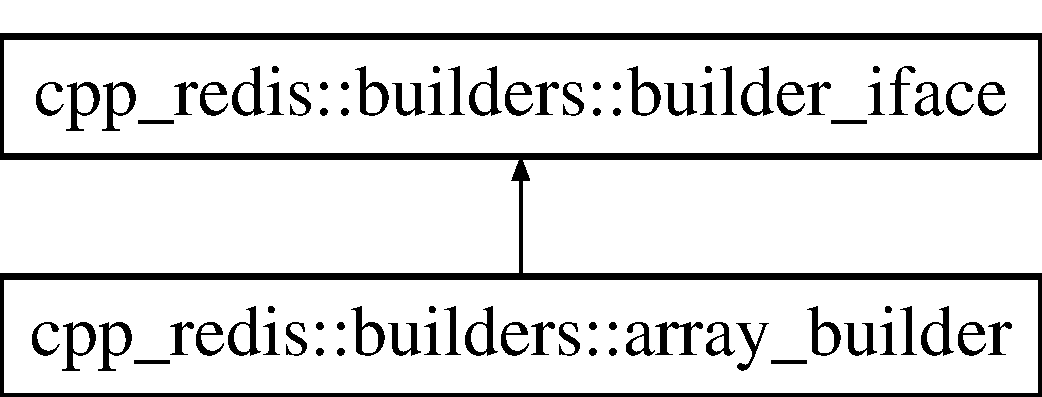
\includegraphics[height=2.000000cm]{classcpp__redis_1_1builders_1_1array__builder}
\end{center}
\end{figure}
\subsection*{Public Member Functions}
\begin{DoxyCompactItemize}
\item 
\hyperlink{classcpp__redis_1_1builders_1_1array__builder_a4beae33a547d3d7efc112659411a23a3}{array\+\_\+builder} (void)
\begin{DoxyCompactList}\small\item\em ctor \end{DoxyCompactList}\item 
\hyperlink{classcpp__redis_1_1builders_1_1array__builder_ae6a0cd0743b6b0a21f9c3d44fd31ac17}{$\sim$array\+\_\+builder} (void)=default
\begin{DoxyCompactList}\small\item\em dtor \end{DoxyCompactList}\item 
\hyperlink{classcpp__redis_1_1builders_1_1array__builder_aa0e5fe9a587b277a473d66b7e6db9548}{array\+\_\+builder} (const \hyperlink{classcpp__redis_1_1builders_1_1array__builder}{array\+\_\+builder} \&)=delete
\begin{DoxyCompactList}\small\item\em copy ctor \end{DoxyCompactList}\item 
\hyperlink{classcpp__redis_1_1builders_1_1array__builder}{array\+\_\+builder} \& \hyperlink{classcpp__redis_1_1builders_1_1array__builder_aaa1df845df7a007cf73f95f73e800c2c}{operator=} (const \hyperlink{classcpp__redis_1_1builders_1_1array__builder}{array\+\_\+builder} \&)=delete
\begin{DoxyCompactList}\small\item\em assignment operator \end{DoxyCompactList}\item 
\hyperlink{classcpp__redis_1_1builders_1_1builder__iface}{builder\+\_\+iface} \& \hyperlink{classcpp__redis_1_1builders_1_1array__builder_a043357d0ef70406adef4df78c8d5307f}{operator$<$$<$} (std\+::string \&data)
\item 
bool \hyperlink{classcpp__redis_1_1builders_1_1array__builder_a524f2cb943dde1246dea1b7057e6351e}{reply\+\_\+ready} (void) const
\item 
\hyperlink{classcpp__redis_1_1reply}{reply} \hyperlink{classcpp__redis_1_1builders_1_1array__builder_ac5c805ad87b357a9578c5a0d479109b3}{get\+\_\+reply} (void) const
\end{DoxyCompactItemize}
\subsection*{Private Member Functions}
\begin{DoxyCompactItemize}
\item 
bool \hyperlink{classcpp__redis_1_1builders_1_1array__builder_a1592420664b191c9133ed364fcb40aa0}{fetch\+\_\+array\+\_\+size} (std\+::string \&buffer)
\item 
bool \hyperlink{classcpp__redis_1_1builders_1_1array__builder_a89c6df1f961723051f3338bdd54a6a9f}{build\+\_\+row} (std\+::string \&buffer)
\end{DoxyCompactItemize}
\subsection*{Private Attributes}
\begin{DoxyCompactItemize}
\item 
\hyperlink{classcpp__redis_1_1builders_1_1integer__builder}{integer\+\_\+builder} \hyperlink{classcpp__redis_1_1builders_1_1array__builder_ac6bafe30792cf577dcb935872056e202}{m\+\_\+int\+\_\+builder}
\item 
uint64\+\_\+t \hyperlink{classcpp__redis_1_1builders_1_1array__builder_a980dc47bd2821608b6399ecf2972262f}{m\+\_\+array\+\_\+size}
\item 
std\+::unique\+\_\+ptr$<$ \hyperlink{classcpp__redis_1_1builders_1_1builder__iface}{builder\+\_\+iface} $>$ \hyperlink{classcpp__redis_1_1builders_1_1array__builder_a6efd7cea5b52fa7750a76906ce520948}{m\+\_\+current\+\_\+builder}
\item 
bool \hyperlink{classcpp__redis_1_1builders_1_1array__builder_ae3b3164237244adc58ffe1fb94946899}{m\+\_\+reply\+\_\+ready}
\item 
\hyperlink{classcpp__redis_1_1reply}{reply} \hyperlink{classcpp__redis_1_1builders_1_1array__builder_a0250a43d8954e282464805b490a6585f}{m\+\_\+reply}
\end{DoxyCompactItemize}


\subsection{Detailed Description}
builder to build redis array replies 

\subsection{Constructor \& Destructor Documentation}
\mbox{\Hypertarget{classcpp__redis_1_1builders_1_1array__builder_a4beae33a547d3d7efc112659411a23a3}\label{classcpp__redis_1_1builders_1_1array__builder_a4beae33a547d3d7efc112659411a23a3}} 
\index{cpp\+\_\+redis\+::builders\+::array\+\_\+builder@{cpp\+\_\+redis\+::builders\+::array\+\_\+builder}!array\+\_\+builder@{array\+\_\+builder}}
\index{array\+\_\+builder@{array\+\_\+builder}!cpp\+\_\+redis\+::builders\+::array\+\_\+builder@{cpp\+\_\+redis\+::builders\+::array\+\_\+builder}}
\subsubsection{\texorpdfstring{array\+\_\+builder()}{array\_builder()}\hspace{0.1cm}{\footnotesize\ttfamily [1/2]}}
{\footnotesize\ttfamily cpp\+\_\+redis\+::builders\+::array\+\_\+builder\+::array\+\_\+builder (\begin{DoxyParamCaption}\item[{void}]{ }\end{DoxyParamCaption})}



ctor 

\mbox{\Hypertarget{classcpp__redis_1_1builders_1_1array__builder_ae6a0cd0743b6b0a21f9c3d44fd31ac17}\label{classcpp__redis_1_1builders_1_1array__builder_ae6a0cd0743b6b0a21f9c3d44fd31ac17}} 
\index{cpp\+\_\+redis\+::builders\+::array\+\_\+builder@{cpp\+\_\+redis\+::builders\+::array\+\_\+builder}!````~array\+\_\+builder@{$\sim$array\+\_\+builder}}
\index{````~array\+\_\+builder@{$\sim$array\+\_\+builder}!cpp\+\_\+redis\+::builders\+::array\+\_\+builder@{cpp\+\_\+redis\+::builders\+::array\+\_\+builder}}
\subsubsection{\texorpdfstring{$\sim$array\+\_\+builder()}{~array\_builder()}}
{\footnotesize\ttfamily cpp\+\_\+redis\+::builders\+::array\+\_\+builder\+::$\sim$array\+\_\+builder (\begin{DoxyParamCaption}\item[{void}]{ }\end{DoxyParamCaption})\hspace{0.3cm}{\ttfamily [default]}}



dtor 

\mbox{\Hypertarget{classcpp__redis_1_1builders_1_1array__builder_aa0e5fe9a587b277a473d66b7e6db9548}\label{classcpp__redis_1_1builders_1_1array__builder_aa0e5fe9a587b277a473d66b7e6db9548}} 
\index{cpp\+\_\+redis\+::builders\+::array\+\_\+builder@{cpp\+\_\+redis\+::builders\+::array\+\_\+builder}!array\+\_\+builder@{array\+\_\+builder}}
\index{array\+\_\+builder@{array\+\_\+builder}!cpp\+\_\+redis\+::builders\+::array\+\_\+builder@{cpp\+\_\+redis\+::builders\+::array\+\_\+builder}}
\subsubsection{\texorpdfstring{array\+\_\+builder()}{array\_builder()}\hspace{0.1cm}{\footnotesize\ttfamily [2/2]}}
{\footnotesize\ttfamily cpp\+\_\+redis\+::builders\+::array\+\_\+builder\+::array\+\_\+builder (\begin{DoxyParamCaption}\item[{const \hyperlink{classcpp__redis_1_1builders_1_1array__builder}{array\+\_\+builder} \&}]{ }\end{DoxyParamCaption})\hspace{0.3cm}{\ttfamily [delete]}}



copy ctor 



\subsection{Member Function Documentation}
\mbox{\Hypertarget{classcpp__redis_1_1builders_1_1array__builder_a89c6df1f961723051f3338bdd54a6a9f}\label{classcpp__redis_1_1builders_1_1array__builder_a89c6df1f961723051f3338bdd54a6a9f}} 
\index{cpp\+\_\+redis\+::builders\+::array\+\_\+builder@{cpp\+\_\+redis\+::builders\+::array\+\_\+builder}!build\+\_\+row@{build\+\_\+row}}
\index{build\+\_\+row@{build\+\_\+row}!cpp\+\_\+redis\+::builders\+::array\+\_\+builder@{cpp\+\_\+redis\+::builders\+::array\+\_\+builder}}
\subsubsection{\texorpdfstring{build\+\_\+row()}{build\_row()}}
{\footnotesize\ttfamily bool cpp\+\_\+redis\+::builders\+::array\+\_\+builder\+::build\+\_\+row (\begin{DoxyParamCaption}\item[{std\+::string \&}]{buffer }\end{DoxyParamCaption})\hspace{0.3cm}{\ttfamily [private]}}

take data as parameter which is consumed to build an array row every bytes used to build row is removed from the buffer passed as parameter


\begin{DoxyParams}{Parameters}
{\em buffer} & data to be consumer \\
\hline
\end{DoxyParams}
\begin{DoxyReturn}{Returns}
true if the row could be built 
\end{DoxyReturn}
\mbox{\Hypertarget{classcpp__redis_1_1builders_1_1array__builder_a1592420664b191c9133ed364fcb40aa0}\label{classcpp__redis_1_1builders_1_1array__builder_a1592420664b191c9133ed364fcb40aa0}} 
\index{cpp\+\_\+redis\+::builders\+::array\+\_\+builder@{cpp\+\_\+redis\+::builders\+::array\+\_\+builder}!fetch\+\_\+array\+\_\+size@{fetch\+\_\+array\+\_\+size}}
\index{fetch\+\_\+array\+\_\+size@{fetch\+\_\+array\+\_\+size}!cpp\+\_\+redis\+::builders\+::array\+\_\+builder@{cpp\+\_\+redis\+::builders\+::array\+\_\+builder}}
\subsubsection{\texorpdfstring{fetch\+\_\+array\+\_\+size()}{fetch\_array\_size()}}
{\footnotesize\ttfamily bool cpp\+\_\+redis\+::builders\+::array\+\_\+builder\+::fetch\+\_\+array\+\_\+size (\begin{DoxyParamCaption}\item[{std\+::string \&}]{buffer }\end{DoxyParamCaption})\hspace{0.3cm}{\ttfamily [private]}}

take data as parameter which is consumed to determine array size every bytes used to build size is removed from the buffer passed as parameter


\begin{DoxyParams}{Parameters}
{\em buffer} & data to be consumer \\
\hline
\end{DoxyParams}
\begin{DoxyReturn}{Returns}
true if the size could be found 
\end{DoxyReturn}
\mbox{\Hypertarget{classcpp__redis_1_1builders_1_1array__builder_ac5c805ad87b357a9578c5a0d479109b3}\label{classcpp__redis_1_1builders_1_1array__builder_ac5c805ad87b357a9578c5a0d479109b3}} 
\index{cpp\+\_\+redis\+::builders\+::array\+\_\+builder@{cpp\+\_\+redis\+::builders\+::array\+\_\+builder}!get\+\_\+reply@{get\+\_\+reply}}
\index{get\+\_\+reply@{get\+\_\+reply}!cpp\+\_\+redis\+::builders\+::array\+\_\+builder@{cpp\+\_\+redis\+::builders\+::array\+\_\+builder}}
\subsubsection{\texorpdfstring{get\+\_\+reply()}{get\_reply()}}
{\footnotesize\ttfamily \hyperlink{classcpp__redis_1_1reply}{reply} cpp\+\_\+redis\+::builders\+::array\+\_\+builder\+::get\+\_\+reply (\begin{DoxyParamCaption}\item[{void}]{ }\end{DoxyParamCaption}) const\hspace{0.3cm}{\ttfamily [virtual]}}

\begin{DoxyReturn}{Returns}
reply object 
\end{DoxyReturn}


Implements \hyperlink{classcpp__redis_1_1builders_1_1builder__iface_afd2ff2c2371c2a486116543b638b9413}{cpp\+\_\+redis\+::builders\+::builder\+\_\+iface}.

\mbox{\Hypertarget{classcpp__redis_1_1builders_1_1array__builder_a043357d0ef70406adef4df78c8d5307f}\label{classcpp__redis_1_1builders_1_1array__builder_a043357d0ef70406adef4df78c8d5307f}} 
\index{cpp\+\_\+redis\+::builders\+::array\+\_\+builder@{cpp\+\_\+redis\+::builders\+::array\+\_\+builder}!operator$<$$<$@{operator$<$$<$}}
\index{operator$<$$<$@{operator$<$$<$}!cpp\+\_\+redis\+::builders\+::array\+\_\+builder@{cpp\+\_\+redis\+::builders\+::array\+\_\+builder}}
\subsubsection{\texorpdfstring{operator$<$$<$()}{operator<<()}}
{\footnotesize\ttfamily \hyperlink{classcpp__redis_1_1builders_1_1builder__iface}{builder\+\_\+iface}\& cpp\+\_\+redis\+::builders\+::array\+\_\+builder\+::operator$<$$<$ (\begin{DoxyParamCaption}\item[{std\+::string \&}]{data }\end{DoxyParamCaption})\hspace{0.3cm}{\ttfamily [virtual]}}

take data as parameter which is consumed to build the reply every bytes used to build the reply must be removed from the buffer passed as parameter


\begin{DoxyParams}{Parameters}
{\em data} & data to be consumed \\
\hline
\end{DoxyParams}
\begin{DoxyReturn}{Returns}
current instance 
\end{DoxyReturn}


Implements \hyperlink{classcpp__redis_1_1builders_1_1builder__iface_a9892bbc9c887c31c2742dad4476e2fa6}{cpp\+\_\+redis\+::builders\+::builder\+\_\+iface}.

\mbox{\Hypertarget{classcpp__redis_1_1builders_1_1array__builder_aaa1df845df7a007cf73f95f73e800c2c}\label{classcpp__redis_1_1builders_1_1array__builder_aaa1df845df7a007cf73f95f73e800c2c}} 
\index{cpp\+\_\+redis\+::builders\+::array\+\_\+builder@{cpp\+\_\+redis\+::builders\+::array\+\_\+builder}!operator=@{operator=}}
\index{operator=@{operator=}!cpp\+\_\+redis\+::builders\+::array\+\_\+builder@{cpp\+\_\+redis\+::builders\+::array\+\_\+builder}}
\subsubsection{\texorpdfstring{operator=()}{operator=()}}
{\footnotesize\ttfamily \hyperlink{classcpp__redis_1_1builders_1_1array__builder}{array\+\_\+builder}\& cpp\+\_\+redis\+::builders\+::array\+\_\+builder\+::operator= (\begin{DoxyParamCaption}\item[{const \hyperlink{classcpp__redis_1_1builders_1_1array__builder}{array\+\_\+builder} \&}]{ }\end{DoxyParamCaption})\hspace{0.3cm}{\ttfamily [delete]}}



assignment operator 

\mbox{\Hypertarget{classcpp__redis_1_1builders_1_1array__builder_a524f2cb943dde1246dea1b7057e6351e}\label{classcpp__redis_1_1builders_1_1array__builder_a524f2cb943dde1246dea1b7057e6351e}} 
\index{cpp\+\_\+redis\+::builders\+::array\+\_\+builder@{cpp\+\_\+redis\+::builders\+::array\+\_\+builder}!reply\+\_\+ready@{reply\+\_\+ready}}
\index{reply\+\_\+ready@{reply\+\_\+ready}!cpp\+\_\+redis\+::builders\+::array\+\_\+builder@{cpp\+\_\+redis\+::builders\+::array\+\_\+builder}}
\subsubsection{\texorpdfstring{reply\+\_\+ready()}{reply\_ready()}}
{\footnotesize\ttfamily bool cpp\+\_\+redis\+::builders\+::array\+\_\+builder\+::reply\+\_\+ready (\begin{DoxyParamCaption}\item[{void}]{ }\end{DoxyParamCaption}) const\hspace{0.3cm}{\ttfamily [virtual]}}

\begin{DoxyReturn}{Returns}
whether the reply could be built 
\end{DoxyReturn}


Implements \hyperlink{classcpp__redis_1_1builders_1_1builder__iface_a40db9a31d4ea1771777e74146d31e12d}{cpp\+\_\+redis\+::builders\+::builder\+\_\+iface}.



\subsection{Member Data Documentation}
\mbox{\Hypertarget{classcpp__redis_1_1builders_1_1array__builder_a980dc47bd2821608b6399ecf2972262f}\label{classcpp__redis_1_1builders_1_1array__builder_a980dc47bd2821608b6399ecf2972262f}} 
\index{cpp\+\_\+redis\+::builders\+::array\+\_\+builder@{cpp\+\_\+redis\+::builders\+::array\+\_\+builder}!m\+\_\+array\+\_\+size@{m\+\_\+array\+\_\+size}}
\index{m\+\_\+array\+\_\+size@{m\+\_\+array\+\_\+size}!cpp\+\_\+redis\+::builders\+::array\+\_\+builder@{cpp\+\_\+redis\+::builders\+::array\+\_\+builder}}
\subsubsection{\texorpdfstring{m\+\_\+array\+\_\+size}{m\_array\_size}}
{\footnotesize\ttfamily uint64\+\_\+t cpp\+\_\+redis\+::builders\+::array\+\_\+builder\+::m\+\_\+array\+\_\+size\hspace{0.3cm}{\ttfamily [private]}}

built array size \mbox{\Hypertarget{classcpp__redis_1_1builders_1_1array__builder_a6efd7cea5b52fa7750a76906ce520948}\label{classcpp__redis_1_1builders_1_1array__builder_a6efd7cea5b52fa7750a76906ce520948}} 
\index{cpp\+\_\+redis\+::builders\+::array\+\_\+builder@{cpp\+\_\+redis\+::builders\+::array\+\_\+builder}!m\+\_\+current\+\_\+builder@{m\+\_\+current\+\_\+builder}}
\index{m\+\_\+current\+\_\+builder@{m\+\_\+current\+\_\+builder}!cpp\+\_\+redis\+::builders\+::array\+\_\+builder@{cpp\+\_\+redis\+::builders\+::array\+\_\+builder}}
\subsubsection{\texorpdfstring{m\+\_\+current\+\_\+builder}{m\_current\_builder}}
{\footnotesize\ttfamily std\+::unique\+\_\+ptr$<$\hyperlink{classcpp__redis_1_1builders_1_1builder__iface}{builder\+\_\+iface}$>$ cpp\+\_\+redis\+::builders\+::array\+\_\+builder\+::m\+\_\+current\+\_\+builder\hspace{0.3cm}{\ttfamily [private]}}

current builder used to build current row \mbox{\Hypertarget{classcpp__redis_1_1builders_1_1array__builder_ac6bafe30792cf577dcb935872056e202}\label{classcpp__redis_1_1builders_1_1array__builder_ac6bafe30792cf577dcb935872056e202}} 
\index{cpp\+\_\+redis\+::builders\+::array\+\_\+builder@{cpp\+\_\+redis\+::builders\+::array\+\_\+builder}!m\+\_\+int\+\_\+builder@{m\+\_\+int\+\_\+builder}}
\index{m\+\_\+int\+\_\+builder@{m\+\_\+int\+\_\+builder}!cpp\+\_\+redis\+::builders\+::array\+\_\+builder@{cpp\+\_\+redis\+::builders\+::array\+\_\+builder}}
\subsubsection{\texorpdfstring{m\+\_\+int\+\_\+builder}{m\_int\_builder}}
{\footnotesize\ttfamily \hyperlink{classcpp__redis_1_1builders_1_1integer__builder}{integer\+\_\+builder} cpp\+\_\+redis\+::builders\+::array\+\_\+builder\+::m\+\_\+int\+\_\+builder\hspace{0.3cm}{\ttfamily [private]}}

builder used to fetch the array size \mbox{\Hypertarget{classcpp__redis_1_1builders_1_1array__builder_a0250a43d8954e282464805b490a6585f}\label{classcpp__redis_1_1builders_1_1array__builder_a0250a43d8954e282464805b490a6585f}} 
\index{cpp\+\_\+redis\+::builders\+::array\+\_\+builder@{cpp\+\_\+redis\+::builders\+::array\+\_\+builder}!m\+\_\+reply@{m\+\_\+reply}}
\index{m\+\_\+reply@{m\+\_\+reply}!cpp\+\_\+redis\+::builders\+::array\+\_\+builder@{cpp\+\_\+redis\+::builders\+::array\+\_\+builder}}
\subsubsection{\texorpdfstring{m\+\_\+reply}{m\_reply}}
{\footnotesize\ttfamily \hyperlink{classcpp__redis_1_1reply}{reply} cpp\+\_\+redis\+::builders\+::array\+\_\+builder\+::m\+\_\+reply\hspace{0.3cm}{\ttfamily [private]}}

reply to be built (or built) \mbox{\Hypertarget{classcpp__redis_1_1builders_1_1array__builder_ae3b3164237244adc58ffe1fb94946899}\label{classcpp__redis_1_1builders_1_1array__builder_ae3b3164237244adc58ffe1fb94946899}} 
\index{cpp\+\_\+redis\+::builders\+::array\+\_\+builder@{cpp\+\_\+redis\+::builders\+::array\+\_\+builder}!m\+\_\+reply\+\_\+ready@{m\+\_\+reply\+\_\+ready}}
\index{m\+\_\+reply\+\_\+ready@{m\+\_\+reply\+\_\+ready}!cpp\+\_\+redis\+::builders\+::array\+\_\+builder@{cpp\+\_\+redis\+::builders\+::array\+\_\+builder}}
\subsubsection{\texorpdfstring{m\+\_\+reply\+\_\+ready}{m\_reply\_ready}}
{\footnotesize\ttfamily bool cpp\+\_\+redis\+::builders\+::array\+\_\+builder\+::m\+\_\+reply\+\_\+ready\hspace{0.3cm}{\ttfamily [private]}}

whether the reply is ready or not 

The documentation for this class was generated from the following file\+:\begin{DoxyCompactItemize}
\item 
includes/cpp\+\_\+redis/builders/\hyperlink{array__builder_8hpp}{array\+\_\+builder.\+hpp}\end{DoxyCompactItemize}

\hypertarget{structcpp__redis_1_1helpers_1_1back}{}\section{cpp\+\_\+redis\+:\+:helpers\+:\+:back$<$ T, Args $>$ Struct Template Reference}
\label{structcpp__redis_1_1helpers_1_1back}\index{cpp\+\_\+redis\+::helpers\+::back$<$ T, Args $>$@{cpp\+\_\+redis\+::helpers\+::back$<$ T, Args $>$}}


{\ttfamily \#include $<$variadic\+\_\+template.\+hpp$>$}

\subsection*{Public Types}
\begin{DoxyCompactItemize}
\item 
using \hyperlink{structcpp__redis_1_1helpers_1_1back_a83f1d0c03ffc82ff8ab7243c3c858195}{type} = typename \hyperlink{structcpp__redis_1_1helpers_1_1back}{back}$<$ Args... $>$\+::\hyperlink{structcpp__redis_1_1helpers_1_1back_a83f1d0c03ffc82ff8ab7243c3c858195}{type}
\end{DoxyCompactItemize}


\subsection{Detailed Description}
\subsubsection*{template$<$typename T, typename... Args$>$\newline
struct cpp\+\_\+redis\+::helpers\+::back$<$ T, Args $>$}

type traits to return last element of a variadic list 

\subsection{Member Typedef Documentation}
\mbox{\Hypertarget{structcpp__redis_1_1helpers_1_1back_a83f1d0c03ffc82ff8ab7243c3c858195}\label{structcpp__redis_1_1helpers_1_1back_a83f1d0c03ffc82ff8ab7243c3c858195}} 
\index{cpp\+\_\+redis\+::helpers\+::back@{cpp\+\_\+redis\+::helpers\+::back}!type@{type}}
\index{type@{type}!cpp\+\_\+redis\+::helpers\+::back@{cpp\+\_\+redis\+::helpers\+::back}}
\subsubsection{\texorpdfstring{type}{type}}
{\footnotesize\ttfamily template$<$typename T , typename... Args$>$ \\
using \hyperlink{structcpp__redis_1_1helpers_1_1back}{cpp\+\_\+redis\+::helpers\+::back}$<$ T, Args $>$\+::\hyperlink{structcpp__redis_1_1helpers_1_1back_a83f1d0c03ffc82ff8ab7243c3c858195}{type} =  typename \hyperlink{structcpp__redis_1_1helpers_1_1back}{back}$<$Args...$>$\+::\hyperlink{structcpp__redis_1_1helpers_1_1back_a83f1d0c03ffc82ff8ab7243c3c858195}{type}}



The documentation for this struct was generated from the following file\+:\begin{DoxyCompactItemize}
\item 
includes/cpp\+\_\+redis/helpers/\hyperlink{variadic__template_8hpp}{variadic\+\_\+template.\+hpp}\end{DoxyCompactItemize}

\hypertarget{structcpp__redis_1_1helpers_1_1back_3_01_t_01_4}{}\section{cpp\+\_\+redis\+:\+:helpers\+:\+:back$<$ T $>$ Struct Template Reference}
\label{structcpp__redis_1_1helpers_1_1back_3_01_t_01_4}\index{cpp\+\_\+redis\+::helpers\+::back$<$ T $>$@{cpp\+\_\+redis\+::helpers\+::back$<$ T $>$}}


{\ttfamily \#include $<$variadic\+\_\+template.\+hpp$>$}

\subsection*{Public Types}
\begin{DoxyCompactItemize}
\item 
using \hyperlink{structcpp__redis_1_1helpers_1_1back_3_01_t_01_4_a87d10cfacd8ca29b083dc5688e77f87c}{type} = T
\end{DoxyCompactItemize}


\subsection{Detailed Description}
\subsubsection*{template$<$typename T$>$\newline
struct cpp\+\_\+redis\+::helpers\+::back$<$ T $>$}

type traits to return last element of a variadic list 

\subsection{Member Typedef Documentation}
\mbox{\Hypertarget{structcpp__redis_1_1helpers_1_1back_3_01_t_01_4_a87d10cfacd8ca29b083dc5688e77f87c}\label{structcpp__redis_1_1helpers_1_1back_3_01_t_01_4_a87d10cfacd8ca29b083dc5688e77f87c}} 
\index{cpp\+\_\+redis\+::helpers\+::back$<$ T $>$@{cpp\+\_\+redis\+::helpers\+::back$<$ T $>$}!type@{type}}
\index{type@{type}!cpp\+\_\+redis\+::helpers\+::back$<$ T $>$@{cpp\+\_\+redis\+::helpers\+::back$<$ T $>$}}
\subsubsection{\texorpdfstring{type}{type}}
{\footnotesize\ttfamily template$<$typename T $>$ \\
using \hyperlink{structcpp__redis_1_1helpers_1_1back}{cpp\+\_\+redis\+::helpers\+::back}$<$ T $>$\+::\hyperlink{structcpp__redis_1_1helpers_1_1back_3_01_t_01_4_a87d10cfacd8ca29b083dc5688e77f87c}{type} =  T}

templated type 

The documentation for this struct was generated from the following file\+:\begin{DoxyCompactItemize}
\item 
includes/cpp\+\_\+redis/helpers/variadic\+\_\+template.\+hpp\end{DoxyCompactItemize}

\hypertarget{structcpp__redis_1_1client_1_1bitfield__operation}{}\section{cpp\+\_\+redis\+:\+:client\+:\+:bitfield\+\_\+operation Struct Reference}
\label{structcpp__redis_1_1client_1_1bitfield__operation}\index{cpp\+\_\+redis\+::client\+::bitfield\+\_\+operation@{cpp\+\_\+redis\+::client\+::bitfield\+\_\+operation}}


{\ttfamily \#include $<$client.\+hpp$>$}

\subsection*{Static Public Member Functions}
\begin{DoxyCompactItemize}
\item 
static \hyperlink{structcpp__redis_1_1client_1_1bitfield__operation}{bitfield\+\_\+operation} \hyperlink{structcpp__redis_1_1client_1_1bitfield__operation_a93d3f7ab6b6bae82ac209bb49374d788}{get} (const std\+::string \&\hyperlink{structcpp__redis_1_1client_1_1bitfield__operation_adbbf30e5138d0524940d536b2bc71480}{type}, int \hyperlink{structcpp__redis_1_1client_1_1bitfield__operation_a8a4e83ddbac5c3500c6960f54e736598}{offset}, \hyperlink{classcpp__redis_1_1client_a4119182ad3a01c1bb626a174375e114a}{overflow\+\_\+type} \hyperlink{structcpp__redis_1_1client_1_1bitfield__operation_a2f478e17655a249080178034faa0f6f2}{overflow}=overflow\+\_\+type\+::server\+\_\+default)
\item 
static \hyperlink{structcpp__redis_1_1client_1_1bitfield__operation}{bitfield\+\_\+operation} \hyperlink{structcpp__redis_1_1client_1_1bitfield__operation_a422fc09f99579cea5fcbcbc3464cdd4e}{set} (const std\+::string \&\hyperlink{structcpp__redis_1_1client_1_1bitfield__operation_adbbf30e5138d0524940d536b2bc71480}{type}, int \hyperlink{structcpp__redis_1_1client_1_1bitfield__operation_a8a4e83ddbac5c3500c6960f54e736598}{offset}, int \hyperlink{structcpp__redis_1_1client_1_1bitfield__operation_a8104441f6b9ee7cbf5e6ee6c17c7445c}{value}, \hyperlink{classcpp__redis_1_1client_a4119182ad3a01c1bb626a174375e114a}{overflow\+\_\+type} \hyperlink{structcpp__redis_1_1client_1_1bitfield__operation_a2f478e17655a249080178034faa0f6f2}{overflow}=overflow\+\_\+type\+::server\+\_\+default)
\item 
static \hyperlink{structcpp__redis_1_1client_1_1bitfield__operation}{bitfield\+\_\+operation} \hyperlink{structcpp__redis_1_1client_1_1bitfield__operation_a9e3ad296a689764917df9da1424f33d5}{incrby} (const std\+::string \&\hyperlink{structcpp__redis_1_1client_1_1bitfield__operation_adbbf30e5138d0524940d536b2bc71480}{type}, int \hyperlink{structcpp__redis_1_1client_1_1bitfield__operation_a8a4e83ddbac5c3500c6960f54e736598}{offset}, int increment, \hyperlink{classcpp__redis_1_1client_a4119182ad3a01c1bb626a174375e114a}{overflow\+\_\+type} \hyperlink{structcpp__redis_1_1client_1_1bitfield__operation_a2f478e17655a249080178034faa0f6f2}{overflow}=overflow\+\_\+type\+::server\+\_\+default)
\end{DoxyCompactItemize}
\subsection*{Public Attributes}
\begin{DoxyCompactItemize}
\item 
\hyperlink{classcpp__redis_1_1client_a2e2023534299541da0a659802e2f087d}{bitfield\+\_\+operation\+\_\+type} \hyperlink{structcpp__redis_1_1client_1_1bitfield__operation_a4f3462e48d5f01b6fcd1605d6de21a3e}{operation\+\_\+type}
\item 
std\+::string \hyperlink{structcpp__redis_1_1client_1_1bitfield__operation_adbbf30e5138d0524940d536b2bc71480}{type}
\item 
int \hyperlink{structcpp__redis_1_1client_1_1bitfield__operation_a8a4e83ddbac5c3500c6960f54e736598}{offset}
\item 
int \hyperlink{structcpp__redis_1_1client_1_1bitfield__operation_a8104441f6b9ee7cbf5e6ee6c17c7445c}{value}
\item 
\hyperlink{classcpp__redis_1_1client_a4119182ad3a01c1bb626a174375e114a}{overflow\+\_\+type} \hyperlink{structcpp__redis_1_1client_1_1bitfield__operation_a2f478e17655a249080178034faa0f6f2}{overflow}
\end{DoxyCompactItemize}


\subsection{Detailed Description}
used to store a get, set or incrby bitfield operation (for bitfield command) 

\subsection{Member Function Documentation}
\mbox{\Hypertarget{structcpp__redis_1_1client_1_1bitfield__operation_a93d3f7ab6b6bae82ac209bb49374d788}\label{structcpp__redis_1_1client_1_1bitfield__operation_a93d3f7ab6b6bae82ac209bb49374d788}} 
\index{cpp\+\_\+redis\+::client\+::bitfield\+\_\+operation@{cpp\+\_\+redis\+::client\+::bitfield\+\_\+operation}!get@{get}}
\index{get@{get}!cpp\+\_\+redis\+::client\+::bitfield\+\_\+operation@{cpp\+\_\+redis\+::client\+::bitfield\+\_\+operation}}
\subsubsection{\texorpdfstring{get()}{get()}}
{\footnotesize\ttfamily static \hyperlink{structcpp__redis_1_1client_1_1bitfield__operation}{bitfield\+\_\+operation} cpp\+\_\+redis\+::client\+::bitfield\+\_\+operation\+::get (\begin{DoxyParamCaption}\item[{const std\+::string \&}]{type,  }\item[{int}]{offset,  }\item[{\hyperlink{classcpp__redis_1_1client_a4119182ad3a01c1bb626a174375e114a}{overflow\+\_\+type}}]{overflow = {\ttfamily overflow\+\_\+type\+:\+:server\+\_\+default} }\end{DoxyParamCaption})\hspace{0.3cm}{\ttfamily [static]}}

build a \hyperlink{structcpp__redis_1_1client_1_1bitfield__operation}{bitfield\+\_\+operation} for a bitfield get operation


\begin{DoxyParams}{Parameters}
{\em type} & type param of a get operation \\
\hline
{\em offset} & offset param of a get operation \\
\hline
{\em overflow} & overflow specification (leave to server\+\_\+default if you do not want to specify it) \\
\hline
\end{DoxyParams}
\begin{DoxyReturn}{Returns}
corresponding get \hyperlink{structcpp__redis_1_1client_1_1bitfield__operation}{bitfield\+\_\+operation} 
\end{DoxyReturn}
\mbox{\Hypertarget{structcpp__redis_1_1client_1_1bitfield__operation_a9e3ad296a689764917df9da1424f33d5}\label{structcpp__redis_1_1client_1_1bitfield__operation_a9e3ad296a689764917df9da1424f33d5}} 
\index{cpp\+\_\+redis\+::client\+::bitfield\+\_\+operation@{cpp\+\_\+redis\+::client\+::bitfield\+\_\+operation}!incrby@{incrby}}
\index{incrby@{incrby}!cpp\+\_\+redis\+::client\+::bitfield\+\_\+operation@{cpp\+\_\+redis\+::client\+::bitfield\+\_\+operation}}
\subsubsection{\texorpdfstring{incrby()}{incrby()}}
{\footnotesize\ttfamily static \hyperlink{structcpp__redis_1_1client_1_1bitfield__operation}{bitfield\+\_\+operation} cpp\+\_\+redis\+::client\+::bitfield\+\_\+operation\+::incrby (\begin{DoxyParamCaption}\item[{const std\+::string \&}]{type,  }\item[{int}]{offset,  }\item[{int}]{increment,  }\item[{\hyperlink{classcpp__redis_1_1client_a4119182ad3a01c1bb626a174375e114a}{overflow\+\_\+type}}]{overflow = {\ttfamily overflow\+\_\+type\+:\+:server\+\_\+default} }\end{DoxyParamCaption})\hspace{0.3cm}{\ttfamily [static]}}

build a \hyperlink{structcpp__redis_1_1client_1_1bitfield__operation}{bitfield\+\_\+operation} for a bitfield incrby operation


\begin{DoxyParams}{Parameters}
{\em type} & type param of a incrby operation \\
\hline
{\em offset} & offset param of a incrby operation \\
\hline
{\em increment} & increment param of a incrby operation \\
\hline
{\em overflow} & overflow specification (leave to server\+\_\+default if you do not want to specify it) \\
\hline
\end{DoxyParams}
\begin{DoxyReturn}{Returns}
corresponding incrby \hyperlink{structcpp__redis_1_1client_1_1bitfield__operation}{bitfield\+\_\+operation} 
\end{DoxyReturn}
\mbox{\Hypertarget{structcpp__redis_1_1client_1_1bitfield__operation_a422fc09f99579cea5fcbcbc3464cdd4e}\label{structcpp__redis_1_1client_1_1bitfield__operation_a422fc09f99579cea5fcbcbc3464cdd4e}} 
\index{cpp\+\_\+redis\+::client\+::bitfield\+\_\+operation@{cpp\+\_\+redis\+::client\+::bitfield\+\_\+operation}!set@{set}}
\index{set@{set}!cpp\+\_\+redis\+::client\+::bitfield\+\_\+operation@{cpp\+\_\+redis\+::client\+::bitfield\+\_\+operation}}
\subsubsection{\texorpdfstring{set()}{set()}}
{\footnotesize\ttfamily static \hyperlink{structcpp__redis_1_1client_1_1bitfield__operation}{bitfield\+\_\+operation} cpp\+\_\+redis\+::client\+::bitfield\+\_\+operation\+::set (\begin{DoxyParamCaption}\item[{const std\+::string \&}]{type,  }\item[{int}]{offset,  }\item[{int}]{value,  }\item[{\hyperlink{classcpp__redis_1_1client_a4119182ad3a01c1bb626a174375e114a}{overflow\+\_\+type}}]{overflow = {\ttfamily overflow\+\_\+type\+:\+:server\+\_\+default} }\end{DoxyParamCaption})\hspace{0.3cm}{\ttfamily [static]}}

build a \hyperlink{structcpp__redis_1_1client_1_1bitfield__operation}{bitfield\+\_\+operation} for a bitfield set operation


\begin{DoxyParams}{Parameters}
{\em type} & type param of a set operation \\
\hline
{\em offset} & offset param of a set operation \\
\hline
{\em value} & value param of a set operation \\
\hline
{\em overflow} & overflow specification (leave to server\+\_\+default if you do not want to specify it) \\
\hline
\end{DoxyParams}
\begin{DoxyReturn}{Returns}
corresponding set \hyperlink{structcpp__redis_1_1client_1_1bitfield__operation}{bitfield\+\_\+operation} 
\end{DoxyReturn}


\subsection{Member Data Documentation}
\mbox{\Hypertarget{structcpp__redis_1_1client_1_1bitfield__operation_a8a4e83ddbac5c3500c6960f54e736598}\label{structcpp__redis_1_1client_1_1bitfield__operation_a8a4e83ddbac5c3500c6960f54e736598}} 
\index{cpp\+\_\+redis\+::client\+::bitfield\+\_\+operation@{cpp\+\_\+redis\+::client\+::bitfield\+\_\+operation}!offset@{offset}}
\index{offset@{offset}!cpp\+\_\+redis\+::client\+::bitfield\+\_\+operation@{cpp\+\_\+redis\+::client\+::bitfield\+\_\+operation}}
\subsubsection{\texorpdfstring{offset}{offset}}
{\footnotesize\ttfamily int cpp\+\_\+redis\+::client\+::bitfield\+\_\+operation\+::offset}

redis offset parameter for get, set or incrby operations \mbox{\Hypertarget{structcpp__redis_1_1client_1_1bitfield__operation_a4f3462e48d5f01b6fcd1605d6de21a3e}\label{structcpp__redis_1_1client_1_1bitfield__operation_a4f3462e48d5f01b6fcd1605d6de21a3e}} 
\index{cpp\+\_\+redis\+::client\+::bitfield\+\_\+operation@{cpp\+\_\+redis\+::client\+::bitfield\+\_\+operation}!operation\+\_\+type@{operation\+\_\+type}}
\index{operation\+\_\+type@{operation\+\_\+type}!cpp\+\_\+redis\+::client\+::bitfield\+\_\+operation@{cpp\+\_\+redis\+::client\+::bitfield\+\_\+operation}}
\subsubsection{\texorpdfstring{operation\+\_\+type}{operation\_type}}
{\footnotesize\ttfamily \hyperlink{classcpp__redis_1_1client_a2e2023534299541da0a659802e2f087d}{bitfield\+\_\+operation\+\_\+type} cpp\+\_\+redis\+::client\+::bitfield\+\_\+operation\+::operation\+\_\+type}

operation type (get, set, incrby) \mbox{\Hypertarget{structcpp__redis_1_1client_1_1bitfield__operation_a2f478e17655a249080178034faa0f6f2}\label{structcpp__redis_1_1client_1_1bitfield__operation_a2f478e17655a249080178034faa0f6f2}} 
\index{cpp\+\_\+redis\+::client\+::bitfield\+\_\+operation@{cpp\+\_\+redis\+::client\+::bitfield\+\_\+operation}!overflow@{overflow}}
\index{overflow@{overflow}!cpp\+\_\+redis\+::client\+::bitfield\+\_\+operation@{cpp\+\_\+redis\+::client\+::bitfield\+\_\+operation}}
\subsubsection{\texorpdfstring{overflow}{overflow}}
{\footnotesize\ttfamily \hyperlink{classcpp__redis_1_1client_a4119182ad3a01c1bb626a174375e114a}{overflow\+\_\+type} cpp\+\_\+redis\+::client\+::bitfield\+\_\+operation\+::overflow}

overflow optional specification \mbox{\Hypertarget{structcpp__redis_1_1client_1_1bitfield__operation_adbbf30e5138d0524940d536b2bc71480}\label{structcpp__redis_1_1client_1_1bitfield__operation_adbbf30e5138d0524940d536b2bc71480}} 
\index{cpp\+\_\+redis\+::client\+::bitfield\+\_\+operation@{cpp\+\_\+redis\+::client\+::bitfield\+\_\+operation}!type@{type}}
\index{type@{type}!cpp\+\_\+redis\+::client\+::bitfield\+\_\+operation@{cpp\+\_\+redis\+::client\+::bitfield\+\_\+operation}}
\subsubsection{\texorpdfstring{type}{type}}
{\footnotesize\ttfamily std\+::string cpp\+\_\+redis\+::client\+::bitfield\+\_\+operation\+::type}

redis type parameter for get, set or incrby operations \mbox{\Hypertarget{structcpp__redis_1_1client_1_1bitfield__operation_a8104441f6b9ee7cbf5e6ee6c17c7445c}\label{structcpp__redis_1_1client_1_1bitfield__operation_a8104441f6b9ee7cbf5e6ee6c17c7445c}} 
\index{cpp\+\_\+redis\+::client\+::bitfield\+\_\+operation@{cpp\+\_\+redis\+::client\+::bitfield\+\_\+operation}!value@{value}}
\index{value@{value}!cpp\+\_\+redis\+::client\+::bitfield\+\_\+operation@{cpp\+\_\+redis\+::client\+::bitfield\+\_\+operation}}
\subsubsection{\texorpdfstring{value}{value}}
{\footnotesize\ttfamily int cpp\+\_\+redis\+::client\+::bitfield\+\_\+operation\+::value}

redis value parameter for set operation, or increment parameter for incrby operation 

The documentation for this struct was generated from the following file\+:\begin{DoxyCompactItemize}
\item 
includes/cpp\+\_\+redis/core/client.\+hpp\end{DoxyCompactItemize}

\hypertarget{classcpp__redis_1_1builders_1_1builder__iface}{}\section{cpp\+\_\+redis\+:\+:builders\+:\+:builder\+\_\+iface Class Reference}
\label{classcpp__redis_1_1builders_1_1builder__iface}\index{cpp\+\_\+redis\+::builders\+::builder\+\_\+iface@{cpp\+\_\+redis\+::builders\+::builder\+\_\+iface}}


{\ttfamily \#include $<$builder\+\_\+iface.\+hpp$>$}

Inheritance diagram for cpp\+\_\+redis\+:\+:builders\+:\+:builder\+\_\+iface\+:\begin{figure}[H]
\begin{center}
\leavevmode
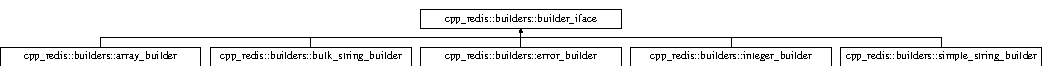
\includegraphics[height=0.888889cm]{classcpp__redis_1_1builders_1_1builder__iface}
\end{center}
\end{figure}
\subsection*{Public Member Functions}
\begin{DoxyCompactItemize}
\item 
virtual \hyperlink{classcpp__redis_1_1builders_1_1builder__iface_afaf3d6cdb3b67b62ed88477dc3d4d1b6}{$\sim$builder\+\_\+iface} (void)=default
\item 
virtual \hyperlink{classcpp__redis_1_1builders_1_1builder__iface}{builder\+\_\+iface} \& \hyperlink{classcpp__redis_1_1builders_1_1builder__iface_a9892bbc9c887c31c2742dad4476e2fa6}{operator$<$$<$} (std\+::string \&data)=0
\item 
virtual bool \hyperlink{classcpp__redis_1_1builders_1_1builder__iface_a40db9a31d4ea1771777e74146d31e12d}{reply\+\_\+ready} (void) const =0
\item 
virtual \hyperlink{classcpp__redis_1_1reply}{reply} \hyperlink{classcpp__redis_1_1builders_1_1builder__iface_afd2ff2c2371c2a486116543b638b9413}{get\+\_\+reply} (void) const =0
\end{DoxyCompactItemize}


\subsection{Detailed Description}
interface inherited by all builders 

\subsection{Constructor \& Destructor Documentation}
\mbox{\Hypertarget{classcpp__redis_1_1builders_1_1builder__iface_afaf3d6cdb3b67b62ed88477dc3d4d1b6}\label{classcpp__redis_1_1builders_1_1builder__iface_afaf3d6cdb3b67b62ed88477dc3d4d1b6}} 
\index{cpp\+\_\+redis\+::builders\+::builder\+\_\+iface@{cpp\+\_\+redis\+::builders\+::builder\+\_\+iface}!````~builder\+\_\+iface@{$\sim$builder\+\_\+iface}}
\index{````~builder\+\_\+iface@{$\sim$builder\+\_\+iface}!cpp\+\_\+redis\+::builders\+::builder\+\_\+iface@{cpp\+\_\+redis\+::builders\+::builder\+\_\+iface}}
\subsubsection{\texorpdfstring{$\sim$builder\+\_\+iface()}{~builder\_iface()}}
{\footnotesize\ttfamily virtual cpp\+\_\+redis\+::builders\+::builder\+\_\+iface\+::$\sim$builder\+\_\+iface (\begin{DoxyParamCaption}\item[{void}]{ }\end{DoxyParamCaption})\hspace{0.3cm}{\ttfamily [virtual]}, {\ttfamily [default]}}



\subsection{Member Function Documentation}
\mbox{\Hypertarget{classcpp__redis_1_1builders_1_1builder__iface_afd2ff2c2371c2a486116543b638b9413}\label{classcpp__redis_1_1builders_1_1builder__iface_afd2ff2c2371c2a486116543b638b9413}} 
\index{cpp\+\_\+redis\+::builders\+::builder\+\_\+iface@{cpp\+\_\+redis\+::builders\+::builder\+\_\+iface}!get\+\_\+reply@{get\+\_\+reply}}
\index{get\+\_\+reply@{get\+\_\+reply}!cpp\+\_\+redis\+::builders\+::builder\+\_\+iface@{cpp\+\_\+redis\+::builders\+::builder\+\_\+iface}}
\subsubsection{\texorpdfstring{get\+\_\+reply()}{get\_reply()}}
{\footnotesize\ttfamily virtual \hyperlink{classcpp__redis_1_1reply}{reply} cpp\+\_\+redis\+::builders\+::builder\+\_\+iface\+::get\+\_\+reply (\begin{DoxyParamCaption}\item[{void}]{ }\end{DoxyParamCaption}) const\hspace{0.3cm}{\ttfamily [pure virtual]}}

\begin{DoxyReturn}{Returns}
reply object 
\end{DoxyReturn}


Implemented in \hyperlink{classcpp__redis_1_1builders_1_1integer__builder_a25221763ba6f8b740458c673945208e0}{cpp\+\_\+redis\+::builders\+::integer\+\_\+builder}, \hyperlink{classcpp__redis_1_1builders_1_1simple__string__builder_a24ad0968d7d02172a65cf8982c540d51}{cpp\+\_\+redis\+::builders\+::simple\+\_\+string\+\_\+builder}, \hyperlink{classcpp__redis_1_1builders_1_1array__builder_ac5c805ad87b357a9578c5a0d479109b3}{cpp\+\_\+redis\+::builders\+::array\+\_\+builder}, \hyperlink{classcpp__redis_1_1builders_1_1bulk__string__builder_a56d6d3089107a1bccd63f6a5267c16cb}{cpp\+\_\+redis\+::builders\+::bulk\+\_\+string\+\_\+builder}, and \hyperlink{classcpp__redis_1_1builders_1_1error__builder_ae2b68b7daad4d71b6780e47bdcc1e32b}{cpp\+\_\+redis\+::builders\+::error\+\_\+builder}.

\mbox{\Hypertarget{classcpp__redis_1_1builders_1_1builder__iface_a9892bbc9c887c31c2742dad4476e2fa6}\label{classcpp__redis_1_1builders_1_1builder__iface_a9892bbc9c887c31c2742dad4476e2fa6}} 
\index{cpp\+\_\+redis\+::builders\+::builder\+\_\+iface@{cpp\+\_\+redis\+::builders\+::builder\+\_\+iface}!operator$<$$<$@{operator$<$$<$}}
\index{operator$<$$<$@{operator$<$$<$}!cpp\+\_\+redis\+::builders\+::builder\+\_\+iface@{cpp\+\_\+redis\+::builders\+::builder\+\_\+iface}}
\subsubsection{\texorpdfstring{operator$<$$<$()}{operator<<()}}
{\footnotesize\ttfamily virtual \hyperlink{classcpp__redis_1_1builders_1_1builder__iface}{builder\+\_\+iface}\& cpp\+\_\+redis\+::builders\+::builder\+\_\+iface\+::operator$<$$<$ (\begin{DoxyParamCaption}\item[{std\+::string \&}]{data }\end{DoxyParamCaption})\hspace{0.3cm}{\ttfamily [pure virtual]}}

take data as parameter which is consumed to build the reply every bytes used to build the reply must be removed from the buffer passed as parameter


\begin{DoxyParams}{Parameters}
{\em data} & data to be consumed \\
\hline
\end{DoxyParams}
\begin{DoxyReturn}{Returns}
current instance 
\end{DoxyReturn}


Implemented in \hyperlink{classcpp__redis_1_1builders_1_1integer__builder_ae29f074134f7269db7f947b0fcbe312e}{cpp\+\_\+redis\+::builders\+::integer\+\_\+builder}, \hyperlink{classcpp__redis_1_1builders_1_1simple__string__builder_a159bb512f0427c4a988742f7cd01035e}{cpp\+\_\+redis\+::builders\+::simple\+\_\+string\+\_\+builder}, \hyperlink{classcpp__redis_1_1builders_1_1array__builder_a043357d0ef70406adef4df78c8d5307f}{cpp\+\_\+redis\+::builders\+::array\+\_\+builder}, \hyperlink{classcpp__redis_1_1builders_1_1bulk__string__builder_a43000357f87212f657aafe279a92b541}{cpp\+\_\+redis\+::builders\+::bulk\+\_\+string\+\_\+builder}, and \hyperlink{classcpp__redis_1_1builders_1_1error__builder_af5ac542be148d6f8500de79fa3164798}{cpp\+\_\+redis\+::builders\+::error\+\_\+builder}.

\mbox{\Hypertarget{classcpp__redis_1_1builders_1_1builder__iface_a40db9a31d4ea1771777e74146d31e12d}\label{classcpp__redis_1_1builders_1_1builder__iface_a40db9a31d4ea1771777e74146d31e12d}} 
\index{cpp\+\_\+redis\+::builders\+::builder\+\_\+iface@{cpp\+\_\+redis\+::builders\+::builder\+\_\+iface}!reply\+\_\+ready@{reply\+\_\+ready}}
\index{reply\+\_\+ready@{reply\+\_\+ready}!cpp\+\_\+redis\+::builders\+::builder\+\_\+iface@{cpp\+\_\+redis\+::builders\+::builder\+\_\+iface}}
\subsubsection{\texorpdfstring{reply\+\_\+ready()}{reply\_ready()}}
{\footnotesize\ttfamily virtual bool cpp\+\_\+redis\+::builders\+::builder\+\_\+iface\+::reply\+\_\+ready (\begin{DoxyParamCaption}\item[{void}]{ }\end{DoxyParamCaption}) const\hspace{0.3cm}{\ttfamily [pure virtual]}}

\begin{DoxyReturn}{Returns}
whether the reply could be built 
\end{DoxyReturn}


Implemented in \hyperlink{classcpp__redis_1_1builders_1_1integer__builder_a4893dc36d06d75094bb4fe3fbc826966}{cpp\+\_\+redis\+::builders\+::integer\+\_\+builder}, \hyperlink{classcpp__redis_1_1builders_1_1simple__string__builder_ad586164caf02b3022b91789cac23a72d}{cpp\+\_\+redis\+::builders\+::simple\+\_\+string\+\_\+builder}, \hyperlink{classcpp__redis_1_1builders_1_1array__builder_a524f2cb943dde1246dea1b7057e6351e}{cpp\+\_\+redis\+::builders\+::array\+\_\+builder}, \hyperlink{classcpp__redis_1_1builders_1_1bulk__string__builder_a4d80d8dfe305e35aca8b4ec84c56fbea}{cpp\+\_\+redis\+::builders\+::bulk\+\_\+string\+\_\+builder}, and \hyperlink{classcpp__redis_1_1builders_1_1error__builder_af3d67647f012d0a7378684e2f8258a6d}{cpp\+\_\+redis\+::builders\+::error\+\_\+builder}.



The documentation for this class was generated from the following file\+:\begin{DoxyCompactItemize}
\item 
includes/cpp\+\_\+redis/builders/\hyperlink{builder__iface_8hpp}{builder\+\_\+iface.\+hpp}\end{DoxyCompactItemize}

\hypertarget{classcpp__redis_1_1builders_1_1bulk__string__builder}{}\section{cpp\+\_\+redis\+:\+:builders\+:\+:bulk\+\_\+string\+\_\+builder Class Reference}
\label{classcpp__redis_1_1builders_1_1bulk__string__builder}\index{cpp\+\_\+redis\+::builders\+::bulk\+\_\+string\+\_\+builder@{cpp\+\_\+redis\+::builders\+::bulk\+\_\+string\+\_\+builder}}


{\ttfamily \#include $<$bulk\+\_\+string\+\_\+builder.\+hpp$>$}

Inheritance diagram for cpp\+\_\+redis\+:\+:builders\+:\+:bulk\+\_\+string\+\_\+builder\+:\begin{figure}[H]
\begin{center}
\leavevmode
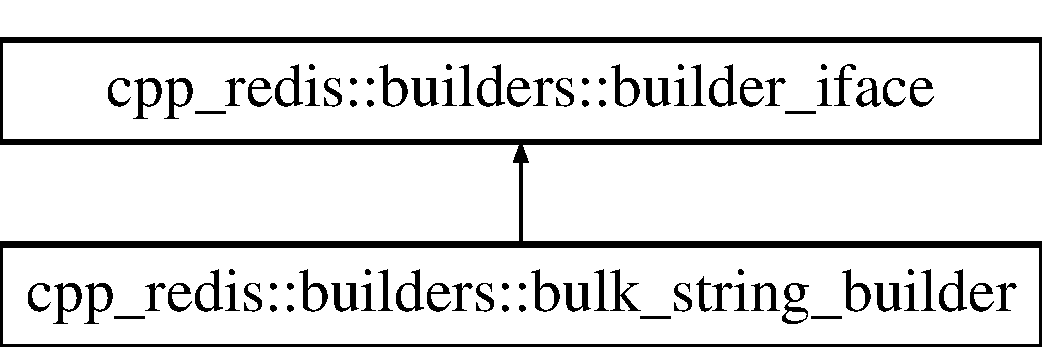
\includegraphics[height=2.000000cm]{classcpp__redis_1_1builders_1_1bulk__string__builder}
\end{center}
\end{figure}
\subsection*{Public Member Functions}
\begin{DoxyCompactItemize}
\item 
\mbox{\Hypertarget{classcpp__redis_1_1builders_1_1bulk__string__builder_a1c0bee3cd6fbafc782cfe93c0b650451}\label{classcpp__redis_1_1builders_1_1bulk__string__builder_a1c0bee3cd6fbafc782cfe93c0b650451}} 
\hyperlink{classcpp__redis_1_1builders_1_1bulk__string__builder_a1c0bee3cd6fbafc782cfe93c0b650451}{bulk\+\_\+string\+\_\+builder} (void)
\begin{DoxyCompactList}\small\item\em ctor \end{DoxyCompactList}\item 
\mbox{\Hypertarget{classcpp__redis_1_1builders_1_1bulk__string__builder_a88c7142bab456f70da9f9a6252e2affb}\label{classcpp__redis_1_1builders_1_1bulk__string__builder_a88c7142bab456f70da9f9a6252e2affb}} 
\hyperlink{classcpp__redis_1_1builders_1_1bulk__string__builder_a88c7142bab456f70da9f9a6252e2affb}{$\sim$bulk\+\_\+string\+\_\+builder} (void)=default
\begin{DoxyCompactList}\small\item\em dtor \end{DoxyCompactList}\item 
\mbox{\Hypertarget{classcpp__redis_1_1builders_1_1bulk__string__builder_ac3bd10f8972fa1856b6e7b7262ecd98f}\label{classcpp__redis_1_1builders_1_1bulk__string__builder_ac3bd10f8972fa1856b6e7b7262ecd98f}} 
\hyperlink{classcpp__redis_1_1builders_1_1bulk__string__builder_ac3bd10f8972fa1856b6e7b7262ecd98f}{bulk\+\_\+string\+\_\+builder} (const \hyperlink{classcpp__redis_1_1builders_1_1bulk__string__builder}{bulk\+\_\+string\+\_\+builder} \&)=delete
\begin{DoxyCompactList}\small\item\em copy ctor \end{DoxyCompactList}\item 
\mbox{\Hypertarget{classcpp__redis_1_1builders_1_1bulk__string__builder_a972355e0910faa9e3daf4f5c67c3e581}\label{classcpp__redis_1_1builders_1_1bulk__string__builder_a972355e0910faa9e3daf4f5c67c3e581}} 
\hyperlink{classcpp__redis_1_1builders_1_1bulk__string__builder}{bulk\+\_\+string\+\_\+builder} \& \hyperlink{classcpp__redis_1_1builders_1_1bulk__string__builder_a972355e0910faa9e3daf4f5c67c3e581}{operator=} (const \hyperlink{classcpp__redis_1_1builders_1_1bulk__string__builder}{bulk\+\_\+string\+\_\+builder} \&)=delete
\begin{DoxyCompactList}\small\item\em assignment operator \end{DoxyCompactList}\item 
\hyperlink{classcpp__redis_1_1builders_1_1builder__iface}{builder\+\_\+iface} \& \hyperlink{classcpp__redis_1_1builders_1_1bulk__string__builder_a43000357f87212f657aafe279a92b541}{operator$<$$<$} (std\+::string \&data)
\item 
bool \hyperlink{classcpp__redis_1_1builders_1_1bulk__string__builder_a4d80d8dfe305e35aca8b4ec84c56fbea}{reply\+\_\+ready} (void) const
\item 
\hyperlink{classcpp__redis_1_1reply}{reply} \hyperlink{classcpp__redis_1_1builders_1_1bulk__string__builder_a56d6d3089107a1bccd63f6a5267c16cb}{get\+\_\+reply} (void) const
\item 
const std\+::string \& \hyperlink{classcpp__redis_1_1builders_1_1bulk__string__builder_a6b3e70acab5c115609db774becbcc571}{get\+\_\+bulk\+\_\+string} (void) const
\item 
bool \hyperlink{classcpp__redis_1_1builders_1_1bulk__string__builder_a2a6ab893dbe5ad2433df18ce62ca6211}{is\+\_\+null} (void) const
\end{DoxyCompactItemize}


\subsection{Detailed Description}
builder to build redis bulk string replies 

\subsection{Member Function Documentation}
\mbox{\Hypertarget{classcpp__redis_1_1builders_1_1bulk__string__builder_a6b3e70acab5c115609db774becbcc571}\label{classcpp__redis_1_1builders_1_1bulk__string__builder_a6b3e70acab5c115609db774becbcc571}} 
\index{cpp\+\_\+redis\+::builders\+::bulk\+\_\+string\+\_\+builder@{cpp\+\_\+redis\+::builders\+::bulk\+\_\+string\+\_\+builder}!get\+\_\+bulk\+\_\+string@{get\+\_\+bulk\+\_\+string}}
\index{get\+\_\+bulk\+\_\+string@{get\+\_\+bulk\+\_\+string}!cpp\+\_\+redis\+::builders\+::bulk\+\_\+string\+\_\+builder@{cpp\+\_\+redis\+::builders\+::bulk\+\_\+string\+\_\+builder}}
\subsubsection{\texorpdfstring{get\+\_\+bulk\+\_\+string()}{get\_bulk\_string()}}
{\footnotesize\ttfamily const std\+::string\& cpp\+\_\+redis\+::builders\+::bulk\+\_\+string\+\_\+builder\+::get\+\_\+bulk\+\_\+string (\begin{DoxyParamCaption}\item[{void}]{ }\end{DoxyParamCaption}) const}

\begin{DoxyReturn}{Returns}
the parsed bulk string 
\end{DoxyReturn}
\mbox{\Hypertarget{classcpp__redis_1_1builders_1_1bulk__string__builder_a56d6d3089107a1bccd63f6a5267c16cb}\label{classcpp__redis_1_1builders_1_1bulk__string__builder_a56d6d3089107a1bccd63f6a5267c16cb}} 
\index{cpp\+\_\+redis\+::builders\+::bulk\+\_\+string\+\_\+builder@{cpp\+\_\+redis\+::builders\+::bulk\+\_\+string\+\_\+builder}!get\+\_\+reply@{get\+\_\+reply}}
\index{get\+\_\+reply@{get\+\_\+reply}!cpp\+\_\+redis\+::builders\+::bulk\+\_\+string\+\_\+builder@{cpp\+\_\+redis\+::builders\+::bulk\+\_\+string\+\_\+builder}}
\subsubsection{\texorpdfstring{get\+\_\+reply()}{get\_reply()}}
{\footnotesize\ttfamily \hyperlink{classcpp__redis_1_1reply}{reply} cpp\+\_\+redis\+::builders\+::bulk\+\_\+string\+\_\+builder\+::get\+\_\+reply (\begin{DoxyParamCaption}\item[{void}]{ }\end{DoxyParamCaption}) const\hspace{0.3cm}{\ttfamily [virtual]}}

\begin{DoxyReturn}{Returns}
reply object 
\end{DoxyReturn}


Implements \hyperlink{classcpp__redis_1_1builders_1_1builder__iface_afd2ff2c2371c2a486116543b638b9413}{cpp\+\_\+redis\+::builders\+::builder\+\_\+iface}.

\mbox{\Hypertarget{classcpp__redis_1_1builders_1_1bulk__string__builder_a2a6ab893dbe5ad2433df18ce62ca6211}\label{classcpp__redis_1_1builders_1_1bulk__string__builder_a2a6ab893dbe5ad2433df18ce62ca6211}} 
\index{cpp\+\_\+redis\+::builders\+::bulk\+\_\+string\+\_\+builder@{cpp\+\_\+redis\+::builders\+::bulk\+\_\+string\+\_\+builder}!is\+\_\+null@{is\+\_\+null}}
\index{is\+\_\+null@{is\+\_\+null}!cpp\+\_\+redis\+::builders\+::bulk\+\_\+string\+\_\+builder@{cpp\+\_\+redis\+::builders\+::bulk\+\_\+string\+\_\+builder}}
\subsubsection{\texorpdfstring{is\+\_\+null()}{is\_null()}}
{\footnotesize\ttfamily bool cpp\+\_\+redis\+::builders\+::bulk\+\_\+string\+\_\+builder\+::is\+\_\+null (\begin{DoxyParamCaption}\item[{void}]{ }\end{DoxyParamCaption}) const}

\begin{DoxyReturn}{Returns}
whether the bulk string is null 
\end{DoxyReturn}
\mbox{\Hypertarget{classcpp__redis_1_1builders_1_1bulk__string__builder_a43000357f87212f657aafe279a92b541}\label{classcpp__redis_1_1builders_1_1bulk__string__builder_a43000357f87212f657aafe279a92b541}} 
\index{cpp\+\_\+redis\+::builders\+::bulk\+\_\+string\+\_\+builder@{cpp\+\_\+redis\+::builders\+::bulk\+\_\+string\+\_\+builder}!operator$<$$<$@{operator$<$$<$}}
\index{operator$<$$<$@{operator$<$$<$}!cpp\+\_\+redis\+::builders\+::bulk\+\_\+string\+\_\+builder@{cpp\+\_\+redis\+::builders\+::bulk\+\_\+string\+\_\+builder}}
\subsubsection{\texorpdfstring{operator$<$$<$()}{operator<<()}}
{\footnotesize\ttfamily \hyperlink{classcpp__redis_1_1builders_1_1builder__iface}{builder\+\_\+iface}\& cpp\+\_\+redis\+::builders\+::bulk\+\_\+string\+\_\+builder\+::operator$<$$<$ (\begin{DoxyParamCaption}\item[{std\+::string \&}]{data }\end{DoxyParamCaption})\hspace{0.3cm}{\ttfamily [virtual]}}

take data as parameter which is consumed to build the reply every bytes used to build the reply must be removed from the buffer passed as parameter


\begin{DoxyParams}{Parameters}
{\em data} & data to be consumed \\
\hline
\end{DoxyParams}
\begin{DoxyReturn}{Returns}
current instance 
\end{DoxyReturn}


Implements \hyperlink{classcpp__redis_1_1builders_1_1builder__iface_a9892bbc9c887c31c2742dad4476e2fa6}{cpp\+\_\+redis\+::builders\+::builder\+\_\+iface}.

\mbox{\Hypertarget{classcpp__redis_1_1builders_1_1bulk__string__builder_a4d80d8dfe305e35aca8b4ec84c56fbea}\label{classcpp__redis_1_1builders_1_1bulk__string__builder_a4d80d8dfe305e35aca8b4ec84c56fbea}} 
\index{cpp\+\_\+redis\+::builders\+::bulk\+\_\+string\+\_\+builder@{cpp\+\_\+redis\+::builders\+::bulk\+\_\+string\+\_\+builder}!reply\+\_\+ready@{reply\+\_\+ready}}
\index{reply\+\_\+ready@{reply\+\_\+ready}!cpp\+\_\+redis\+::builders\+::bulk\+\_\+string\+\_\+builder@{cpp\+\_\+redis\+::builders\+::bulk\+\_\+string\+\_\+builder}}
\subsubsection{\texorpdfstring{reply\+\_\+ready()}{reply\_ready()}}
{\footnotesize\ttfamily bool cpp\+\_\+redis\+::builders\+::bulk\+\_\+string\+\_\+builder\+::reply\+\_\+ready (\begin{DoxyParamCaption}\item[{void}]{ }\end{DoxyParamCaption}) const\hspace{0.3cm}{\ttfamily [virtual]}}

\begin{DoxyReturn}{Returns}
whether the reply could be built 
\end{DoxyReturn}


Implements \hyperlink{classcpp__redis_1_1builders_1_1builder__iface_a40db9a31d4ea1771777e74146d31e12d}{cpp\+\_\+redis\+::builders\+::builder\+\_\+iface}.



The documentation for this class was generated from the following file\+:\begin{DoxyCompactItemize}
\item 
includes/cpp\+\_\+redis/builders/bulk\+\_\+string\+\_\+builder.\+hpp\end{DoxyCompactItemize}

\hypertarget{classcpp__redis_1_1client}{}\section{cpp\+\_\+redis\+:\+:client Class Reference}
\label{classcpp__redis_1_1client}\index{cpp\+\_\+redis\+::client@{cpp\+\_\+redis\+::client}}


{\ttfamily \#include $<$client.\+hpp$>$}

\subsection*{Classes}
\begin{DoxyCompactItemize}
\item 
struct \hyperlink{structcpp__redis_1_1client_1_1command__request}{command\+\_\+request}
\end{DoxyCompactItemize}
\subsection*{Public Types}
\begin{DoxyCompactItemize}
\item 
enum \hyperlink{classcpp__redis_1_1client_a388877b01b4e045cddb138e70a68e000}{client\+\_\+type} \{ \hyperlink{classcpp__redis_1_1client_a388877b01b4e045cddb138e70a68e000afea087517c26fadd409bd4b9dc642555}{client\+\_\+type\+::normal}, 
\hyperlink{classcpp__redis_1_1client_a388877b01b4e045cddb138e70a68e000aeb0a191797624dd3a48fa681d3061212}{client\+\_\+type\+::master}, 
\hyperlink{classcpp__redis_1_1client_a388877b01b4e045cddb138e70a68e000a040f8e6525bd0c62798afb41e6644f37}{client\+\_\+type\+::pubsub}, 
\hyperlink{classcpp__redis_1_1client_a388877b01b4e045cddb138e70a68e000a03158cf39c6f316f9ce98a4e034cdc28}{client\+\_\+type\+::slave}
 \}
\item 
enum \hyperlink{classcpp__redis_1_1client_a2512bd48dd45391249a69bd720c1e4da}{connect\+\_\+state} \{ \newline
\hyperlink{classcpp__redis_1_1client_a2512bd48dd45391249a69bd720c1e4daa41d368a58ee26891a6a586ddaaa604f8}{connect\+\_\+state\+::dropped}, 
\hyperlink{classcpp__redis_1_1client_a2512bd48dd45391249a69bd720c1e4daaea2b2676c28c0db26d39331a336c6b92}{connect\+\_\+state\+::start}, 
\hyperlink{classcpp__redis_1_1client_a2512bd48dd45391249a69bd720c1e4daad98cb5df35fc9e0f42fb883d794ad12f}{connect\+\_\+state\+::sleeping}, 
\hyperlink{classcpp__redis_1_1client_a2512bd48dd45391249a69bd720c1e4daa444bcb3a3fcf8389296c49467f27e1d6}{connect\+\_\+state\+::ok}, 
\newline
\hyperlink{classcpp__redis_1_1client_a2512bd48dd45391249a69bd720c1e4daa26934eb377001f66e37289a5c93fe284}{connect\+\_\+state\+::failed}, 
\hyperlink{classcpp__redis_1_1client_a2512bd48dd45391249a69bd720c1e4daa1c35224aee766403970dfaa34880ccde}{connect\+\_\+state\+::lookup\+\_\+failed}, 
\hyperlink{classcpp__redis_1_1client_a2512bd48dd45391249a69bd720c1e4daaf0a0bfe6bc7d2c58d2989034f83183e0}{connect\+\_\+state\+::stopped}
 \}
\item 
typedef std\+::function$<$ void(const std\+::string \&host, std\+::size\+\_\+t port, \hyperlink{classcpp__redis_1_1client_a2512bd48dd45391249a69bd720c1e4da}{connect\+\_\+state} status)$>$ \hyperlink{classcpp__redis_1_1client_a4bb592b64ededde5a6fcf8111ca2548f}{connect\+\_\+callback\+\_\+t}
\item 
typedef std\+::function$<$ void(\hyperlink{classcpp__redis_1_1reply}{reply} \&)$>$ \hyperlink{classcpp__redis_1_1client_a061a1140d36d2eaeda82b09a0bb3f9f2}{reply\+\_\+callback\+\_\+t}
\end{DoxyCompactItemize}
\subsection*{Public Member Functions}
\begin{DoxyCompactItemize}
\item 
\hyperlink{classcpp__redis_1_1client_a80354f41d084dfc3a41df581c803b792}{client} (void)
\begin{DoxyCompactList}\small\item\em ctor \end{DoxyCompactList}\item 
\hyperlink{classcpp__redis_1_1client_ae879c3a6829a2da9d03f80c1ec4b8d9b}{client} (const std\+::shared\+\_\+ptr$<$ \hyperlink{classcpp__redis_1_1network_1_1tcp__client__iface}{network\+::tcp\+\_\+client\+\_\+iface} $>$ \&tcp\+\_\+client)
\item 
\hyperlink{classcpp__redis_1_1client_aca7030c8bd6856f10314b2862d1bae79}{$\sim$client} (void)
\begin{DoxyCompactList}\small\item\em dtor \end{DoxyCompactList}\item 
\hyperlink{classcpp__redis_1_1client_ab938aeb2a144629fd269594e4af08168}{client} (const \hyperlink{classcpp__redis_1_1client}{client} \&)=delete
\begin{DoxyCompactList}\small\item\em copy ctor \end{DoxyCompactList}\item 
\hyperlink{classcpp__redis_1_1client}{client} \& \hyperlink{classcpp__redis_1_1client_afdab99b1752e759ab3ce9477f2cb092d}{operator=} (const \hyperlink{classcpp__redis_1_1client}{client} \&)=delete
\begin{DoxyCompactList}\small\item\em assignment operator \end{DoxyCompactList}\item 
void \hyperlink{classcpp__redis_1_1client_adda8b3e7b4f9c80ac052753b39178dd5}{connect} (const std\+::string \&host=\char`\"{}127.\+0.\+0.\+1\char`\"{}, std\+::size\+\_\+t port=6379, const \hyperlink{classcpp__redis_1_1client_a4bb592b64ededde5a6fcf8111ca2548f}{connect\+\_\+callback\+\_\+t} \&connect\+\_\+callback=nullptr, std\+::uint32\+\_\+t timeout\+\_\+msecs=0, std\+::int32\+\_\+t max\+\_\+reconnects=0, std\+::uint32\+\_\+t reconnect\+\_\+interval\+\_\+msecs=0)
\item 
void \hyperlink{classcpp__redis_1_1client_a15bcb0885129480543482a7da52af892}{connect} (const std\+::string \&name, const \hyperlink{classcpp__redis_1_1client_a4bb592b64ededde5a6fcf8111ca2548f}{connect\+\_\+callback\+\_\+t} \&connect\+\_\+callback=nullptr, std\+::uint32\+\_\+t timeout\+\_\+msecs=0, std\+::int32\+\_\+t max\+\_\+reconnects=0, std\+::uint32\+\_\+t reconnect\+\_\+interval\+\_\+msecs=0)
\item 
bool \hyperlink{classcpp__redis_1_1client_ad3608dec2c2bfabf2c621ce14f4db37a}{is\+\_\+connected} (void) const
\item 
void \hyperlink{classcpp__redis_1_1client_a292252b61bcfdf9ad3854b54b7fe2740}{disconnect} (bool wait\+\_\+for\+\_\+removal=false)
\item 
bool \hyperlink{classcpp__redis_1_1client_af03ca1aec6416ab35e6aea93c74d89d1}{is\+\_\+reconnecting} (void) const
\item 
void \hyperlink{classcpp__redis_1_1client_adb605a877f65b8f54725576b45aeeca6}{cancel\+\_\+reconnect} (void)
\item 
\hyperlink{classcpp__redis_1_1client}{client} \& \hyperlink{classcpp__redis_1_1client_a490ef812b666e6d845fcacc808b87bc1}{send} (const std\+::vector$<$ std\+::string $>$ \&redis\+\_\+cmd, const \hyperlink{classcpp__redis_1_1client_a061a1140d36d2eaeda82b09a0bb3f9f2}{reply\+\_\+callback\+\_\+t} \&callback)
\item 
std\+::future$<$ \hyperlink{classcpp__redis_1_1reply}{reply} $>$ \hyperlink{classcpp__redis_1_1client_ad6216d6587d50694c16d68e8e182b0be}{send} (const std\+::vector$<$ std\+::string $>$ \&redis\+\_\+cmd)
\item 
\hyperlink{classcpp__redis_1_1client}{client} \& \hyperlink{classcpp__redis_1_1client_a36a48d61a4900e88fd67795ca59cbea3}{commit} (void)
\item 
\hyperlink{classcpp__redis_1_1client}{client} \& \hyperlink{classcpp__redis_1_1client_a23c8a27ee691c52713411ae91e1391fb}{sync\+\_\+commit} (void)
\item 
{\footnotesize template$<$class Rep , class Period $>$ }\\\hyperlink{classcpp__redis_1_1client}{client} \& \hyperlink{classcpp__redis_1_1client_a79a24c8367cb1229fd2c4c38d0f82533}{sync\+\_\+commit} (const std\+::chrono\+::duration$<$ Rep, Period $>$ \&timeout)
\item 
void \hyperlink{classcpp__redis_1_1client_a7050eb52856decad9ab2060a139f4b48}{add\+\_\+sentinel} (const std\+::string \&host, std\+::size\+\_\+t port)
\item 
void \hyperlink{classcpp__redis_1_1client_a68cd15d1cc30302237e3a400e2ac43f5}{clear\+\_\+sentinels} (void)
\item 
\hyperlink{classcpp__redis_1_1client}{client} \& \hyperlink{classcpp__redis_1_1client_ad60647638d8758103e98894457652b84}{append} (const std\+::string \&key, const std\+::string \&value, const \hyperlink{classcpp__redis_1_1client_a061a1140d36d2eaeda82b09a0bb3f9f2}{reply\+\_\+callback\+\_\+t} \&reply\+\_\+callback)
\item 
std\+::future$<$ \hyperlink{classcpp__redis_1_1reply}{reply} $>$ \hyperlink{classcpp__redis_1_1client_a3e50dddad0b4c9eca58d970bdc4e78da}{append} (const std\+::string \&key, const std\+::string \&value)
\item 
\hyperlink{classcpp__redis_1_1client}{client} \& \hyperlink{classcpp__redis_1_1client_a3ee834ca9c0810d2eafcf04de9dc0670}{auth} (const std\+::string \&password, const \hyperlink{classcpp__redis_1_1client_a061a1140d36d2eaeda82b09a0bb3f9f2}{reply\+\_\+callback\+\_\+t} \&reply\+\_\+callback)
\item 
std\+::future$<$ \hyperlink{classcpp__redis_1_1reply}{reply} $>$ \hyperlink{classcpp__redis_1_1client_a899b98d4d6da0ffdf8780933fe088fd1}{auth} (const std\+::string \&password)
\item 
\hyperlink{classcpp__redis_1_1client}{client} \& \hyperlink{classcpp__redis_1_1client_a9873619c2c1ff820fde17e27ade096c8}{bgrewriteaof} (const \hyperlink{classcpp__redis_1_1client_a061a1140d36d2eaeda82b09a0bb3f9f2}{reply\+\_\+callback\+\_\+t} \&reply\+\_\+callback)
\item 
std\+::future$<$ \hyperlink{classcpp__redis_1_1reply}{reply} $>$ \hyperlink{classcpp__redis_1_1client_a82959607f4cbe9dac195d27621a9cc64}{bgrewriteaof} ()
\item 
\hyperlink{classcpp__redis_1_1client}{client} \& \hyperlink{classcpp__redis_1_1client_a102a4f3572072a5bc26681082ad16a2b}{bgsave} (const \hyperlink{classcpp__redis_1_1client_a061a1140d36d2eaeda82b09a0bb3f9f2}{reply\+\_\+callback\+\_\+t} \&reply\+\_\+callback)
\item 
std\+::future$<$ \hyperlink{classcpp__redis_1_1reply}{reply} $>$ \hyperlink{classcpp__redis_1_1client_a632ef40c52f46eb4948768006adfead5}{bgsave} ()
\item 
\hyperlink{classcpp__redis_1_1client}{client} \& \hyperlink{classcpp__redis_1_1client_aa6c9c15d8676a1cee3d8409ab898a049}{bitcount} (const std\+::string \&key, const \hyperlink{classcpp__redis_1_1client_a061a1140d36d2eaeda82b09a0bb3f9f2}{reply\+\_\+callback\+\_\+t} \&reply\+\_\+callback)
\item 
std\+::future$<$ \hyperlink{classcpp__redis_1_1reply}{reply} $>$ \hyperlink{classcpp__redis_1_1client_ac667b96661726874bc237c84de1ddd89}{bitcount} (const std\+::string \&key)
\item 
\hyperlink{classcpp__redis_1_1client}{client} \& \hyperlink{classcpp__redis_1_1client_ac631a06c8b69a2f1b4de3aabc19d68e2}{bitcount} (const std\+::string \&key, int start, int end, const \hyperlink{classcpp__redis_1_1client_a061a1140d36d2eaeda82b09a0bb3f9f2}{reply\+\_\+callback\+\_\+t} \&reply\+\_\+callback)
\item 
std\+::future$<$ \hyperlink{classcpp__redis_1_1reply}{reply} $>$ \hyperlink{classcpp__redis_1_1client_af2d2dc1c19d735e84d8e2725fb98dbda}{bitcount} (const std\+::string \&key, int start, int end)
\item 
\hyperlink{classcpp__redis_1_1client}{client} \& \hyperlink{classcpp__redis_1_1client_a9289b0f474073f59509b565d93c69506}{bitop} (const std\+::string \&operation, const std\+::string \&destkey, const std\+::vector$<$ std\+::string $>$ \&\hyperlink{classcpp__redis_1_1client_acb7845a206b2321e6919c2f38282c322}{keys}, const \hyperlink{classcpp__redis_1_1client_a061a1140d36d2eaeda82b09a0bb3f9f2}{reply\+\_\+callback\+\_\+t} \&reply\+\_\+callback)
\item 
std\+::future$<$ \hyperlink{classcpp__redis_1_1reply}{reply} $>$ \hyperlink{classcpp__redis_1_1client_adbb955ee435dea43898ef811b31421b3}{bitop} (const std\+::string \&operation, const std\+::string \&destkey, const std\+::vector$<$ std\+::string $>$ \&\hyperlink{classcpp__redis_1_1client_acb7845a206b2321e6919c2f38282c322}{keys})
\item 
\hyperlink{classcpp__redis_1_1client}{client} \& \hyperlink{classcpp__redis_1_1client_adf2ef5d020a8efbf6f6eb91cde63f262}{bitpos} (const std\+::string \&key, int bit, const \hyperlink{classcpp__redis_1_1client_a061a1140d36d2eaeda82b09a0bb3f9f2}{reply\+\_\+callback\+\_\+t} \&reply\+\_\+callback)
\item 
std\+::future$<$ \hyperlink{classcpp__redis_1_1reply}{reply} $>$ \hyperlink{classcpp__redis_1_1client_a5be47a4b3f9a36c4fab420468d50256a}{bitpos} (const std\+::string \&key, int bit)
\item 
\hyperlink{classcpp__redis_1_1client}{client} \& \hyperlink{classcpp__redis_1_1client_a8f6b7958a3094c975c3ca053b263c523}{bitpos} (const std\+::string \&key, int bit, int start, const \hyperlink{classcpp__redis_1_1client_a061a1140d36d2eaeda82b09a0bb3f9f2}{reply\+\_\+callback\+\_\+t} \&reply\+\_\+callback)
\item 
std\+::future$<$ \hyperlink{classcpp__redis_1_1reply}{reply} $>$ \hyperlink{classcpp__redis_1_1client_aa0ae004e45eb37ffed4d8c9f5ea35b4c}{bitpos} (const std\+::string \&key, int bit, int start)
\item 
\hyperlink{classcpp__redis_1_1client}{client} \& \hyperlink{classcpp__redis_1_1client_a3655449a666a9111d3dce7e61932ab1b}{bitpos} (const std\+::string \&key, int bit, int start, int end, const \hyperlink{classcpp__redis_1_1client_a061a1140d36d2eaeda82b09a0bb3f9f2}{reply\+\_\+callback\+\_\+t} \&reply\+\_\+callback)
\item 
std\+::future$<$ \hyperlink{classcpp__redis_1_1reply}{reply} $>$ \hyperlink{classcpp__redis_1_1client_a43b5121105276ccae731bb6093c80e02}{bitpos} (const std\+::string \&key, int bit, int start, int end)
\item 
\hyperlink{classcpp__redis_1_1client}{client} \& \hyperlink{classcpp__redis_1_1client_a432c2677b13dc8e2a9d7afe7eade39e3}{blpop} (const std\+::vector$<$ std\+::string $>$ \&\hyperlink{classcpp__redis_1_1client_acb7845a206b2321e6919c2f38282c322}{keys}, int timeout, const \hyperlink{classcpp__redis_1_1client_a061a1140d36d2eaeda82b09a0bb3f9f2}{reply\+\_\+callback\+\_\+t} \&reply\+\_\+callback)
\item 
std\+::future$<$ \hyperlink{classcpp__redis_1_1reply}{reply} $>$ \hyperlink{classcpp__redis_1_1client_ac54c987bca4efb4bf6659b063f19d5ff}{blpop} (const std\+::vector$<$ std\+::string $>$ \&\hyperlink{classcpp__redis_1_1client_acb7845a206b2321e6919c2f38282c322}{keys}, int timeout)
\item 
\hyperlink{classcpp__redis_1_1client}{client} \& \hyperlink{classcpp__redis_1_1client_adc565332168e31ebbd762f2cb12ad4d1}{brpop} (const std\+::vector$<$ std\+::string $>$ \&\hyperlink{classcpp__redis_1_1client_acb7845a206b2321e6919c2f38282c322}{keys}, int timeout, const \hyperlink{classcpp__redis_1_1client_a061a1140d36d2eaeda82b09a0bb3f9f2}{reply\+\_\+callback\+\_\+t} \&reply\+\_\+callback)
\item 
std\+::future$<$ \hyperlink{classcpp__redis_1_1reply}{reply} $>$ \hyperlink{classcpp__redis_1_1client_aa123b931c6d00027d08f0fcbde2f026e}{brpop} (const std\+::vector$<$ std\+::string $>$ \&\hyperlink{classcpp__redis_1_1client_acb7845a206b2321e6919c2f38282c322}{keys}, int timeout)
\item 
\hyperlink{classcpp__redis_1_1client}{client} \& \hyperlink{classcpp__redis_1_1client_afa7fb97bb0b30c2c78a605f48b6144e2}{brpoplpush} (const std\+::string \&src, const std\+::string \&dst, int timeout, const \hyperlink{classcpp__redis_1_1client_a061a1140d36d2eaeda82b09a0bb3f9f2}{reply\+\_\+callback\+\_\+t} \&reply\+\_\+callback)
\item 
std\+::future$<$ \hyperlink{classcpp__redis_1_1reply}{reply} $>$ \hyperlink{classcpp__redis_1_1client_aa30b9303ee0d59b07dd656db2426547e}{brpoplpush} (const std\+::string \&src, const std\+::string \&dst, int timeout)
\item 
{\footnotesize template$<$typename T , typename... Ts$>$ }\\\hyperlink{classcpp__redis_1_1client}{client} \& \hyperlink{classcpp__redis_1_1client_ae4090830d1710276c33ff5a74eba2e4b}{client\+\_\+kill} (const std\+::string \&host, int port, const T \&arg, const Ts \&... args)
\item 
\hyperlink{classcpp__redis_1_1client}{client} \& \hyperlink{classcpp__redis_1_1client_a3163e1f29d65a5e7b0d4165be154fb96}{client\+\_\+kill} (const std\+::string \&host, int port)
\item 
{\footnotesize template$<$typename... Ts$>$ }\\\hyperlink{classcpp__redis_1_1client}{client} \& \hyperlink{classcpp__redis_1_1client_a38df8e614a5ac9533a1993b7dec7be6b}{client\+\_\+kill} (const char $\ast$host, int port, const Ts \&... args)
\item 
{\footnotesize template$<$typename T , typename... Ts$>$ }\\\hyperlink{classcpp__redis_1_1client}{client} \& \hyperlink{classcpp__redis_1_1client_a1e2dd6cdcdb4307ceda0f866fe0a154f}{client\+\_\+kill} (const T \&, const Ts \&...)
\item 
{\footnotesize template$<$typename T , typename... Ts$>$ }\\std\+::future$<$ \hyperlink{classcpp__redis_1_1reply}{reply} $>$ \hyperlink{classcpp__redis_1_1client_ae6f09b6c022c910b79fb90a47291f511}{client\+\_\+kill\+\_\+future} (const T, const Ts...)
\item 
\hyperlink{classcpp__redis_1_1client}{client} \& \hyperlink{classcpp__redis_1_1client_a9c2e307ab54f42ce50bdd42e1c6a363b}{client\+\_\+list} (const \hyperlink{classcpp__redis_1_1client_a061a1140d36d2eaeda82b09a0bb3f9f2}{reply\+\_\+callback\+\_\+t} \&reply\+\_\+callback)
\item 
std\+::future$<$ \hyperlink{classcpp__redis_1_1reply}{reply} $>$ \hyperlink{classcpp__redis_1_1client_a0480140cc584e6dd2a0a6fab9da10cc5}{client\+\_\+list} ()
\item 
\hyperlink{classcpp__redis_1_1client}{client} \& \hyperlink{classcpp__redis_1_1client_ac4e058eaa75eb04c7a8017a779d5015e}{client\+\_\+getname} (const \hyperlink{classcpp__redis_1_1client_a061a1140d36d2eaeda82b09a0bb3f9f2}{reply\+\_\+callback\+\_\+t} \&reply\+\_\+callback)
\item 
std\+::future$<$ \hyperlink{classcpp__redis_1_1reply}{reply} $>$ \hyperlink{classcpp__redis_1_1client_a89068e68b418906e9e34cb9a95f7a179}{client\+\_\+getname} ()
\item 
\hyperlink{classcpp__redis_1_1client}{client} \& \hyperlink{classcpp__redis_1_1client_acdf001d60d1d82d3f090b7c679e3183e}{client\+\_\+pause} (int timeout, const \hyperlink{classcpp__redis_1_1client_a061a1140d36d2eaeda82b09a0bb3f9f2}{reply\+\_\+callback\+\_\+t} \&reply\+\_\+callback)
\item 
std\+::future$<$ \hyperlink{classcpp__redis_1_1reply}{reply} $>$ \hyperlink{classcpp__redis_1_1client_a2c73a6f9b2e3f1a0afbaca9fddd29199}{client\+\_\+pause} (int timeout)
\item 
\hyperlink{classcpp__redis_1_1client}{client} \& \hyperlink{classcpp__redis_1_1client_a5e49e9bf9bb72659b33013fac751a712}{client\+\_\+reply} (const std\+::string \&mode, const \hyperlink{classcpp__redis_1_1client_a061a1140d36d2eaeda82b09a0bb3f9f2}{reply\+\_\+callback\+\_\+t} \&reply\+\_\+callback)
\item 
std\+::future$<$ \hyperlink{classcpp__redis_1_1reply}{reply} $>$ \hyperlink{classcpp__redis_1_1client_a1b378de0c1805069b9bbecd4fca4091c}{client\+\_\+reply} (const std\+::string \&mode)
\item 
\hyperlink{classcpp__redis_1_1client}{client} \& \hyperlink{classcpp__redis_1_1client_a5c7f977196c1c00e3c732615c0d86ae7}{client\+\_\+setname} (const std\+::string \&name, const \hyperlink{classcpp__redis_1_1client_a061a1140d36d2eaeda82b09a0bb3f9f2}{reply\+\_\+callback\+\_\+t} \&reply\+\_\+callback)
\item 
std\+::future$<$ \hyperlink{classcpp__redis_1_1reply}{reply} $>$ \hyperlink{classcpp__redis_1_1client_aa1ab41fda6b2536f652720b7720a0b63}{client\+\_\+setname} (const std\+::string \&name)
\item 
\hyperlink{classcpp__redis_1_1client}{client} \& \hyperlink{classcpp__redis_1_1client_ac156d5593e1800742188f0eee9016a84}{cluster\+\_\+addslots} (const std\+::vector$<$ std\+::string $>$ \&p\+\_\+slots, const \hyperlink{classcpp__redis_1_1client_a061a1140d36d2eaeda82b09a0bb3f9f2}{reply\+\_\+callback\+\_\+t} \&reply\+\_\+callback)
\item 
std\+::future$<$ \hyperlink{classcpp__redis_1_1reply}{reply} $>$ \hyperlink{classcpp__redis_1_1client_a0e14578c1addf1de66745a8a95e66aeb}{cluster\+\_\+addslots} (const std\+::vector$<$ std\+::string $>$ \&p\+\_\+slots)
\item 
\hyperlink{classcpp__redis_1_1client}{client} \& \hyperlink{classcpp__redis_1_1client_a757c2a5c8e5b42ccd3930d89d739f602}{cluster\+\_\+count\+\_\+failure\+\_\+reports} (const std\+::string \&node\+\_\+id, const \hyperlink{classcpp__redis_1_1client_a061a1140d36d2eaeda82b09a0bb3f9f2}{reply\+\_\+callback\+\_\+t} \&reply\+\_\+callback)
\item 
std\+::future$<$ \hyperlink{classcpp__redis_1_1reply}{reply} $>$ \hyperlink{classcpp__redis_1_1client_af1ff307eb9feb58b48b11bda78131a20}{cluster\+\_\+count\+\_\+failure\+\_\+reports} (const std\+::string \&node\+\_\+id)
\item 
\hyperlink{classcpp__redis_1_1client}{client} \& \hyperlink{classcpp__redis_1_1client_a78017860625d016074d0495c24c3f9e8}{cluster\+\_\+countkeysinslot} (const std\+::string \&slot, const \hyperlink{classcpp__redis_1_1client_a061a1140d36d2eaeda82b09a0bb3f9f2}{reply\+\_\+callback\+\_\+t} \&reply\+\_\+callback)
\item 
std\+::future$<$ \hyperlink{classcpp__redis_1_1reply}{reply} $>$ \hyperlink{classcpp__redis_1_1client_a8135eee3cfc95b061aee9b6f7271efce}{cluster\+\_\+countkeysinslot} (const std\+::string \&slot)
\item 
\hyperlink{classcpp__redis_1_1client}{client} \& \hyperlink{classcpp__redis_1_1client_a41f96bb9a627724570f1866d0983d7b2}{cluster\+\_\+delslots} (const std\+::vector$<$ std\+::string $>$ \&p\+\_\+slots, const \hyperlink{classcpp__redis_1_1client_a061a1140d36d2eaeda82b09a0bb3f9f2}{reply\+\_\+callback\+\_\+t} \&reply\+\_\+callback)
\item 
std\+::future$<$ \hyperlink{classcpp__redis_1_1reply}{reply} $>$ \hyperlink{classcpp__redis_1_1client_a6cd07520f60ee78c4603211273adcf46}{cluster\+\_\+delslots} (const std\+::vector$<$ std\+::string $>$ \&p\+\_\+slots)
\item 
\hyperlink{classcpp__redis_1_1client}{client} \& \hyperlink{classcpp__redis_1_1client_a5afcee001e210150803a95c3d6412998}{cluster\+\_\+failover} (const \hyperlink{classcpp__redis_1_1client_a061a1140d36d2eaeda82b09a0bb3f9f2}{reply\+\_\+callback\+\_\+t} \&reply\+\_\+callback)
\item 
std\+::future$<$ \hyperlink{classcpp__redis_1_1reply}{reply} $>$ \hyperlink{classcpp__redis_1_1client_a76122bb138c12b90c78c4e511f45ef17}{cluster\+\_\+failover} ()
\item 
\hyperlink{classcpp__redis_1_1client}{client} \& \hyperlink{classcpp__redis_1_1client_a9c95de64e422c09c2180dc69db386d06}{cluster\+\_\+failover} (const std\+::string \&mode, const \hyperlink{classcpp__redis_1_1client_a061a1140d36d2eaeda82b09a0bb3f9f2}{reply\+\_\+callback\+\_\+t} \&reply\+\_\+callback)
\item 
std\+::future$<$ \hyperlink{classcpp__redis_1_1reply}{reply} $>$ \hyperlink{classcpp__redis_1_1client_a06f9c7d27f961787b01a01be95f1fa29}{cluster\+\_\+failover} (const std\+::string \&mode)
\item 
\hyperlink{classcpp__redis_1_1client}{client} \& \hyperlink{classcpp__redis_1_1client_aea8a77acb9031fd03f8ab5dc2c09a17d}{cluster\+\_\+forget} (const std\+::string \&node\+\_\+id, const \hyperlink{classcpp__redis_1_1client_a061a1140d36d2eaeda82b09a0bb3f9f2}{reply\+\_\+callback\+\_\+t} \&reply\+\_\+callback)
\item 
std\+::future$<$ \hyperlink{classcpp__redis_1_1reply}{reply} $>$ \hyperlink{classcpp__redis_1_1client_a58457400352dee764066bd9f737f667a}{cluster\+\_\+forget} (const std\+::string \&node\+\_\+id)
\item 
\hyperlink{classcpp__redis_1_1client}{client} \& \hyperlink{classcpp__redis_1_1client_a716e31987800e3ca5483f72972fecfb0}{cluster\+\_\+getkeysinslot} (const std\+::string \&slot, int count, const \hyperlink{classcpp__redis_1_1client_a061a1140d36d2eaeda82b09a0bb3f9f2}{reply\+\_\+callback\+\_\+t} \&reply\+\_\+callback)
\item 
std\+::future$<$ \hyperlink{classcpp__redis_1_1reply}{reply} $>$ \hyperlink{classcpp__redis_1_1client_ad644ef5c24f3eb51de30a827753cc077}{cluster\+\_\+getkeysinslot} (const std\+::string \&slot, int count)
\item 
\hyperlink{classcpp__redis_1_1client}{client} \& \hyperlink{classcpp__redis_1_1client_a831d52a9dc9115e817bae15db0fb18a6}{cluster\+\_\+info} (const \hyperlink{classcpp__redis_1_1client_a061a1140d36d2eaeda82b09a0bb3f9f2}{reply\+\_\+callback\+\_\+t} \&reply\+\_\+callback)
\item 
std\+::future$<$ \hyperlink{classcpp__redis_1_1reply}{reply} $>$ \hyperlink{classcpp__redis_1_1client_a993170e08c425a810fa757bd4c202d10}{cluster\+\_\+info} ()
\item 
\hyperlink{classcpp__redis_1_1client}{client} \& \hyperlink{classcpp__redis_1_1client_ae0314fc2697674f4be4fca1cc5cbd4a1}{cluster\+\_\+keyslot} (const std\+::string \&key, const \hyperlink{classcpp__redis_1_1client_a061a1140d36d2eaeda82b09a0bb3f9f2}{reply\+\_\+callback\+\_\+t} \&reply\+\_\+callback)
\item 
std\+::future$<$ \hyperlink{classcpp__redis_1_1reply}{reply} $>$ \hyperlink{classcpp__redis_1_1client_a5681ac2dfdacc19cde1a828d8b801df1}{cluster\+\_\+keyslot} (const std\+::string \&key)
\item 
\hyperlink{classcpp__redis_1_1client}{client} \& \hyperlink{classcpp__redis_1_1client_aefc94be1dc7eb11673ba92bc8cbffdcf}{cluster\+\_\+meet} (const std\+::string \&ip, int port, const \hyperlink{classcpp__redis_1_1client_a061a1140d36d2eaeda82b09a0bb3f9f2}{reply\+\_\+callback\+\_\+t} \&reply\+\_\+callback)
\item 
std\+::future$<$ \hyperlink{classcpp__redis_1_1reply}{reply} $>$ \hyperlink{classcpp__redis_1_1client_af142b166d5f88f76f5fd46e6e33c0523}{cluster\+\_\+meet} (const std\+::string \&ip, int port)
\item 
\hyperlink{classcpp__redis_1_1client}{client} \& \hyperlink{classcpp__redis_1_1client_a1e4cc880ce249fcad1b1f6ddd15f515f}{cluster\+\_\+nodes} (const \hyperlink{classcpp__redis_1_1client_a061a1140d36d2eaeda82b09a0bb3f9f2}{reply\+\_\+callback\+\_\+t} \&reply\+\_\+callback)
\item 
std\+::future$<$ \hyperlink{classcpp__redis_1_1reply}{reply} $>$ \hyperlink{classcpp__redis_1_1client_a6e777dc7b54ecb4aff3e1c281f92dd81}{cluster\+\_\+nodes} ()
\item 
\hyperlink{classcpp__redis_1_1client}{client} \& \hyperlink{classcpp__redis_1_1client_a65688223390e47c0400ba4a128000f89}{cluster\+\_\+replicate} (const std\+::string \&node\+\_\+id, const \hyperlink{classcpp__redis_1_1client_a061a1140d36d2eaeda82b09a0bb3f9f2}{reply\+\_\+callback\+\_\+t} \&reply\+\_\+callback)
\item 
std\+::future$<$ \hyperlink{classcpp__redis_1_1reply}{reply} $>$ \hyperlink{classcpp__redis_1_1client_a4ce5b739522aefd5ca7c8aef8c76cc61}{cluster\+\_\+replicate} (const std\+::string \&node\+\_\+id)
\item 
\hyperlink{classcpp__redis_1_1client}{client} \& \hyperlink{classcpp__redis_1_1client_a99c86f1931c92594f2c14ac34b3d5dfd}{cluster\+\_\+reset} (const \hyperlink{classcpp__redis_1_1client_a061a1140d36d2eaeda82b09a0bb3f9f2}{reply\+\_\+callback\+\_\+t} \&reply\+\_\+callback)
\item 
\hyperlink{classcpp__redis_1_1client}{client} \& \hyperlink{classcpp__redis_1_1client_a3f039634232d14d4eec6fea27784a347}{cluster\+\_\+reset} (const std\+::string \&mode, const \hyperlink{classcpp__redis_1_1client_a061a1140d36d2eaeda82b09a0bb3f9f2}{reply\+\_\+callback\+\_\+t} \&reply\+\_\+callback)
\item 
std\+::future$<$ \hyperlink{classcpp__redis_1_1reply}{reply} $>$ \hyperlink{classcpp__redis_1_1client_ac49706b4ea17538653a6e5a77791ae31}{cluster\+\_\+reset} (const std\+::string \&mode=\char`\"{}soft\char`\"{})
\item 
\hyperlink{classcpp__redis_1_1client}{client} \& \hyperlink{classcpp__redis_1_1client_a2860dbeb1f7acd44e72e3ad02fc16e20}{cluster\+\_\+saveconfig} (const \hyperlink{classcpp__redis_1_1client_a061a1140d36d2eaeda82b09a0bb3f9f2}{reply\+\_\+callback\+\_\+t} \&reply\+\_\+callback)
\item 
std\+::future$<$ \hyperlink{classcpp__redis_1_1reply}{reply} $>$ \hyperlink{classcpp__redis_1_1client_a5b8571b48e9e56fad203a04dd50559be}{cluster\+\_\+saveconfig} ()
\item 
\hyperlink{classcpp__redis_1_1client}{client} \& \hyperlink{classcpp__redis_1_1client_ac930f6544459b0b2476f741beb6a2508}{cluster\+\_\+set\+\_\+config\+\_\+epoch} (const std\+::string \&epoch, const \hyperlink{classcpp__redis_1_1client_a061a1140d36d2eaeda82b09a0bb3f9f2}{reply\+\_\+callback\+\_\+t} \&reply\+\_\+callback)
\item 
std\+::future$<$ \hyperlink{classcpp__redis_1_1reply}{reply} $>$ \hyperlink{classcpp__redis_1_1client_a0be11e04ce58a13e2e40272be1fad788}{cluster\+\_\+set\+\_\+config\+\_\+epoch} (const std\+::string \&epoch)
\item 
\hyperlink{classcpp__redis_1_1client}{client} \& \hyperlink{classcpp__redis_1_1client_aeba14289869fe871eb9eb9c2503635a8}{cluster\+\_\+setslot} (const std\+::string \&slot, const std\+::string \&mode, const \hyperlink{classcpp__redis_1_1client_a061a1140d36d2eaeda82b09a0bb3f9f2}{reply\+\_\+callback\+\_\+t} \&reply\+\_\+callback)
\item 
std\+::future$<$ \hyperlink{classcpp__redis_1_1reply}{reply} $>$ \hyperlink{classcpp__redis_1_1client_ad9b75e2c90b1b87fa93a3ac76bd1512f}{cluster\+\_\+setslot} (const std\+::string \&slot, const std\+::string \&mode)
\item 
\hyperlink{classcpp__redis_1_1client}{client} \& \hyperlink{classcpp__redis_1_1client_a4e87a3163d16db267136a127e5c843e2}{cluster\+\_\+setslot} (const std\+::string \&slot, const std\+::string \&mode, const std\+::string \&node\+\_\+id, const \hyperlink{classcpp__redis_1_1client_a061a1140d36d2eaeda82b09a0bb3f9f2}{reply\+\_\+callback\+\_\+t} \&reply\+\_\+callback)
\item 
std\+::future$<$ \hyperlink{classcpp__redis_1_1reply}{reply} $>$ \hyperlink{classcpp__redis_1_1client_a824c1234198e48badeccf4190b610e32}{cluster\+\_\+setslot} (const std\+::string \&slot, const std\+::string \&mode, const std\+::string \&node\+\_\+id)
\item 
\hyperlink{classcpp__redis_1_1client}{client} \& \hyperlink{classcpp__redis_1_1client_ac03fb62a9eb5abbb5248bc38fd4dfb5e}{cluster\+\_\+slaves} (const std\+::string \&node\+\_\+id, const \hyperlink{classcpp__redis_1_1client_a061a1140d36d2eaeda82b09a0bb3f9f2}{reply\+\_\+callback\+\_\+t} \&reply\+\_\+callback)
\item 
std\+::future$<$ \hyperlink{classcpp__redis_1_1reply}{reply} $>$ \hyperlink{classcpp__redis_1_1client_afbfca7fb91f492768c7ac75677f433a2}{cluster\+\_\+slaves} (const std\+::string \&node\+\_\+id)
\item 
\hyperlink{classcpp__redis_1_1client}{client} \& \hyperlink{classcpp__redis_1_1client_a7d0dad34ca2fe2e301b202388bb47e10}{cluster\+\_\+slots} (const \hyperlink{classcpp__redis_1_1client_a061a1140d36d2eaeda82b09a0bb3f9f2}{reply\+\_\+callback\+\_\+t} \&reply\+\_\+callback)
\item 
std\+::future$<$ \hyperlink{classcpp__redis_1_1reply}{reply} $>$ \hyperlink{classcpp__redis_1_1client_a9dc222141ab85da05efbce7a7ff0a7d1}{cluster\+\_\+slots} ()
\item 
\hyperlink{classcpp__redis_1_1client}{client} \& \hyperlink{classcpp__redis_1_1client_accac4fab4be3f71b94fc0aa02496f6a3}{command} (const \hyperlink{classcpp__redis_1_1client_a061a1140d36d2eaeda82b09a0bb3f9f2}{reply\+\_\+callback\+\_\+t} \&reply\+\_\+callback)
\item 
std\+::future$<$ \hyperlink{classcpp__redis_1_1reply}{reply} $>$ \hyperlink{classcpp__redis_1_1client_a93ef2e84647990d02aa67a1e22341b38}{command} ()
\item 
\hyperlink{classcpp__redis_1_1client}{client} \& \hyperlink{classcpp__redis_1_1client_a639c7fd5c7899ba474e65513ee337bea}{command\+\_\+count} (const \hyperlink{classcpp__redis_1_1client_a061a1140d36d2eaeda82b09a0bb3f9f2}{reply\+\_\+callback\+\_\+t} \&reply\+\_\+callback)
\item 
std\+::future$<$ \hyperlink{classcpp__redis_1_1reply}{reply} $>$ \hyperlink{classcpp__redis_1_1client_af0cac37a62edbd7d699b379551f1ef9a}{command\+\_\+count} ()
\item 
\hyperlink{classcpp__redis_1_1client}{client} \& \hyperlink{classcpp__redis_1_1client_a3d23ff98ee82a404373d75b660720926}{command\+\_\+getkeys} (const \hyperlink{classcpp__redis_1_1client_a061a1140d36d2eaeda82b09a0bb3f9f2}{reply\+\_\+callback\+\_\+t} \&reply\+\_\+callback)
\item 
std\+::future$<$ \hyperlink{classcpp__redis_1_1reply}{reply} $>$ \hyperlink{classcpp__redis_1_1client_a18ab313316e99ab0a690540f40de80e3}{command\+\_\+getkeys} ()
\item 
\hyperlink{classcpp__redis_1_1client}{client} \& \hyperlink{classcpp__redis_1_1client_a95105c556aa5c070819bc82729d336c5}{command\+\_\+info} (const std\+::vector$<$ std\+::string $>$ \&command\+\_\+name, const \hyperlink{classcpp__redis_1_1client_a061a1140d36d2eaeda82b09a0bb3f9f2}{reply\+\_\+callback\+\_\+t} \&reply\+\_\+callback)
\item 
std\+::future$<$ \hyperlink{classcpp__redis_1_1reply}{reply} $>$ \hyperlink{classcpp__redis_1_1client_abd02a4d296ed0c160e935cd176862334}{command\+\_\+info} (const std\+::vector$<$ std\+::string $>$ \&command\+\_\+name)
\item 
\hyperlink{classcpp__redis_1_1client}{client} \& \hyperlink{classcpp__redis_1_1client_a510ede75cc6361f33a4cdd0695f7543f}{config\+\_\+get} (const std\+::string \&param, const \hyperlink{classcpp__redis_1_1client_a061a1140d36d2eaeda82b09a0bb3f9f2}{reply\+\_\+callback\+\_\+t} \&reply\+\_\+callback)
\item 
std\+::future$<$ \hyperlink{classcpp__redis_1_1reply}{reply} $>$ \hyperlink{classcpp__redis_1_1client_a221b1e414a4b1bb4eb2a7afaac0eb39d}{config\+\_\+get} (const std\+::string \&param)
\item 
\hyperlink{classcpp__redis_1_1client}{client} \& \hyperlink{classcpp__redis_1_1client_a8dcf862a8a0cb75f8cc986445eae81cf}{config\+\_\+rewrite} (const \hyperlink{classcpp__redis_1_1client_a061a1140d36d2eaeda82b09a0bb3f9f2}{reply\+\_\+callback\+\_\+t} \&reply\+\_\+callback)
\item 
std\+::future$<$ \hyperlink{classcpp__redis_1_1reply}{reply} $>$ \hyperlink{classcpp__redis_1_1client_a1a001663bd555abb70521924ec2a27f8}{config\+\_\+rewrite} ()
\item 
\hyperlink{classcpp__redis_1_1client}{client} \& \hyperlink{classcpp__redis_1_1client_a0cff7147cd982a39cc84f91243a27364}{config\+\_\+set} (const std\+::string \&param, const std\+::string \&val, const \hyperlink{classcpp__redis_1_1client_a061a1140d36d2eaeda82b09a0bb3f9f2}{reply\+\_\+callback\+\_\+t} \&reply\+\_\+callback)
\item 
std\+::future$<$ \hyperlink{classcpp__redis_1_1reply}{reply} $>$ \hyperlink{classcpp__redis_1_1client_a8fdeb462b43ea6f5199145696713f9b1}{config\+\_\+set} (const std\+::string \&param, const std\+::string \&val)
\item 
\hyperlink{classcpp__redis_1_1client}{client} \& \hyperlink{classcpp__redis_1_1client_a4b1361aa6c997b76a059c144a302b5be}{config\+\_\+resetstat} (const \hyperlink{classcpp__redis_1_1client_a061a1140d36d2eaeda82b09a0bb3f9f2}{reply\+\_\+callback\+\_\+t} \&reply\+\_\+callback)
\item 
std\+::future$<$ \hyperlink{classcpp__redis_1_1reply}{reply} $>$ \hyperlink{classcpp__redis_1_1client_a775508ce5220546e46b573f95d2bcb4d}{config\+\_\+resetstat} ()
\item 
\hyperlink{classcpp__redis_1_1client}{client} \& \hyperlink{classcpp__redis_1_1client_a87a8351f0a6927db52b4ab2a5b9192c9}{dbsize} (const \hyperlink{classcpp__redis_1_1client_a061a1140d36d2eaeda82b09a0bb3f9f2}{reply\+\_\+callback\+\_\+t} \&reply\+\_\+callback)
\item 
std\+::future$<$ \hyperlink{classcpp__redis_1_1reply}{reply} $>$ \hyperlink{classcpp__redis_1_1client_aa9169c3c4a8b3ec5ee7b7bc601ae8a52}{dbsize} ()
\item 
\hyperlink{classcpp__redis_1_1client}{client} \& \hyperlink{classcpp__redis_1_1client_ad96e4d369e87e858fd7a8296b5cc378e}{debug\+\_\+object} (const std\+::string \&key, const \hyperlink{classcpp__redis_1_1client_a061a1140d36d2eaeda82b09a0bb3f9f2}{reply\+\_\+callback\+\_\+t} \&reply\+\_\+callback)
\item 
std\+::future$<$ \hyperlink{classcpp__redis_1_1reply}{reply} $>$ \hyperlink{classcpp__redis_1_1client_a9d7a2eae091f99db6b5479577de0bf99}{debug\+\_\+object} (const std\+::string \&key)
\item 
\hyperlink{classcpp__redis_1_1client}{client} \& \hyperlink{classcpp__redis_1_1client_ac5d06ca1072ef1a83a8843c448e4d1e3}{debug\+\_\+segfault} (const \hyperlink{classcpp__redis_1_1client_a061a1140d36d2eaeda82b09a0bb3f9f2}{reply\+\_\+callback\+\_\+t} \&reply\+\_\+callback)
\item 
std\+::future$<$ \hyperlink{classcpp__redis_1_1reply}{reply} $>$ \hyperlink{classcpp__redis_1_1client_a764786e7003c538a6cf0a5d6b44d66dd}{debug\+\_\+segfault} ()
\item 
\hyperlink{classcpp__redis_1_1client}{client} \& \hyperlink{classcpp__redis_1_1client_a8e09d5753d9f9ba00b1d5e8aed306189}{decr} (const std\+::string \&key, const \hyperlink{classcpp__redis_1_1client_a061a1140d36d2eaeda82b09a0bb3f9f2}{reply\+\_\+callback\+\_\+t} \&reply\+\_\+callback)
\item 
std\+::future$<$ \hyperlink{classcpp__redis_1_1reply}{reply} $>$ \hyperlink{classcpp__redis_1_1client_ac80abd9a238a7613294d4444bbc92907}{decr} (const std\+::string \&key)
\item 
\hyperlink{classcpp__redis_1_1client}{client} \& \hyperlink{classcpp__redis_1_1client_aaa45a662abeaa66f5a8c985cd27957c8}{decrby} (const std\+::string \&key, int val, const \hyperlink{classcpp__redis_1_1client_a061a1140d36d2eaeda82b09a0bb3f9f2}{reply\+\_\+callback\+\_\+t} \&reply\+\_\+callback)
\item 
std\+::future$<$ \hyperlink{classcpp__redis_1_1reply}{reply} $>$ \hyperlink{classcpp__redis_1_1client_ac4fe81368d7f9cc305811d8346e60881}{decrby} (const std\+::string \&key, int val)
\item 
\hyperlink{classcpp__redis_1_1client}{client} \& \hyperlink{classcpp__redis_1_1client_a29a5307b20d9ffe951e2ff302797a296}{del} (const std\+::vector$<$ std\+::string $>$ \&key, const \hyperlink{classcpp__redis_1_1client_a061a1140d36d2eaeda82b09a0bb3f9f2}{reply\+\_\+callback\+\_\+t} \&reply\+\_\+callback)
\item 
std\+::future$<$ \hyperlink{classcpp__redis_1_1reply}{reply} $>$ \hyperlink{classcpp__redis_1_1client_a99c090de7e23accfaf3b93f4b025d2e9}{del} (const std\+::vector$<$ std\+::string $>$ \&key)
\item 
\hyperlink{classcpp__redis_1_1client}{client} \& \hyperlink{classcpp__redis_1_1client_a0f5a07744750f87504f72dcf66144a24}{discard} (const \hyperlink{classcpp__redis_1_1client_a061a1140d36d2eaeda82b09a0bb3f9f2}{reply\+\_\+callback\+\_\+t} \&reply\+\_\+callback)
\item 
std\+::future$<$ \hyperlink{classcpp__redis_1_1reply}{reply} $>$ \hyperlink{classcpp__redis_1_1client_ab37e125f4f94bfa9455dc29f64698e47}{discard} ()
\item 
\hyperlink{classcpp__redis_1_1client}{client} \& \hyperlink{classcpp__redis_1_1client_aed6bb7657acdd4ea4dd0a4e7ec3eec20}{dump} (const std\+::string \&key, const \hyperlink{classcpp__redis_1_1client_a061a1140d36d2eaeda82b09a0bb3f9f2}{reply\+\_\+callback\+\_\+t} \&reply\+\_\+callback)
\item 
std\+::future$<$ \hyperlink{classcpp__redis_1_1reply}{reply} $>$ \hyperlink{classcpp__redis_1_1client_aa25f7f2648c1a013ce079ef13e8e2f0f}{dump} (const std\+::string \&key)
\item 
\hyperlink{classcpp__redis_1_1client}{client} \& \hyperlink{classcpp__redis_1_1client_a285d35a355052ae1757d13ecec0539e8}{echo} (const std\+::string \&msg, const \hyperlink{classcpp__redis_1_1client_a061a1140d36d2eaeda82b09a0bb3f9f2}{reply\+\_\+callback\+\_\+t} \&reply\+\_\+callback)
\item 
std\+::future$<$ \hyperlink{classcpp__redis_1_1reply}{reply} $>$ \hyperlink{classcpp__redis_1_1client_af0e3462a35f72aeae1527f0cb3cc8570}{echo} (const std\+::string \&msg)
\item 
\hyperlink{classcpp__redis_1_1client}{client} \& \hyperlink{classcpp__redis_1_1client_aeb773d0e0cacb766a0c4c7641bd91ebf}{eval} (const std\+::string \&script, int numkeys, const std\+::vector$<$ std\+::string $>$ \&\hyperlink{classcpp__redis_1_1client_acb7845a206b2321e6919c2f38282c322}{keys}, const std\+::vector$<$ std\+::string $>$ \&args, const \hyperlink{classcpp__redis_1_1client_a061a1140d36d2eaeda82b09a0bb3f9f2}{reply\+\_\+callback\+\_\+t} \&reply\+\_\+callback)
\item 
std\+::future$<$ \hyperlink{classcpp__redis_1_1reply}{reply} $>$ \hyperlink{classcpp__redis_1_1client_a01b328b664e5cf604150e3d0f881ff4c}{eval} (const std\+::string \&script, int numkeys, const std\+::vector$<$ std\+::string $>$ \&\hyperlink{classcpp__redis_1_1client_acb7845a206b2321e6919c2f38282c322}{keys}, const std\+::vector$<$ std\+::string $>$ \&args)
\item 
\hyperlink{classcpp__redis_1_1client}{client} \& \hyperlink{classcpp__redis_1_1client_a71cd73130b4755c9f4da3b602b09a1be}{evalsha} (const std\+::string \&sha1, int numkeys, const std\+::vector$<$ std\+::string $>$ \&\hyperlink{classcpp__redis_1_1client_acb7845a206b2321e6919c2f38282c322}{keys}, const std\+::vector$<$ std\+::string $>$ \&args, const \hyperlink{classcpp__redis_1_1client_a061a1140d36d2eaeda82b09a0bb3f9f2}{reply\+\_\+callback\+\_\+t} \&reply\+\_\+callback)
\item 
std\+::future$<$ \hyperlink{classcpp__redis_1_1reply}{reply} $>$ \hyperlink{classcpp__redis_1_1client_a3ab7684f292037dc3918c32549b7ad53}{evalsha} (const std\+::string \&sha1, int numkeys, const std\+::vector$<$ std\+::string $>$ \&\hyperlink{classcpp__redis_1_1client_acb7845a206b2321e6919c2f38282c322}{keys}, const std\+::vector$<$ std\+::string $>$ \&args)
\item 
\hyperlink{classcpp__redis_1_1client}{client} \& \hyperlink{classcpp__redis_1_1client_a76e78829c4ee2e1484268e465fab8997}{exec} (const \hyperlink{classcpp__redis_1_1client_a061a1140d36d2eaeda82b09a0bb3f9f2}{reply\+\_\+callback\+\_\+t} \&reply\+\_\+callback)
\item 
std\+::future$<$ \hyperlink{classcpp__redis_1_1reply}{reply} $>$ \hyperlink{classcpp__redis_1_1client_a93c5b232ae13b5107b6aa1ea5f70b70d}{exec} ()
\item 
\hyperlink{classcpp__redis_1_1client}{client} \& \hyperlink{classcpp__redis_1_1client_a11836c341d54a9d767cd37508bf87d73}{exists} (const std\+::vector$<$ std\+::string $>$ \&\hyperlink{classcpp__redis_1_1client_acb7845a206b2321e6919c2f38282c322}{keys}, const \hyperlink{classcpp__redis_1_1client_a061a1140d36d2eaeda82b09a0bb3f9f2}{reply\+\_\+callback\+\_\+t} \&reply\+\_\+callback)
\item 
std\+::future$<$ \hyperlink{classcpp__redis_1_1reply}{reply} $>$ \hyperlink{classcpp__redis_1_1client_a16ab72e15bd14a3fd2eb97194cea3d2d}{exists} (const std\+::vector$<$ std\+::string $>$ \&\hyperlink{classcpp__redis_1_1client_acb7845a206b2321e6919c2f38282c322}{keys})
\item 
\hyperlink{classcpp__redis_1_1client}{client} \& \hyperlink{classcpp__redis_1_1client_ab2c50e9f37a4e6a5dff059c991dbd15e}{expire} (const std\+::string \&key, int seconds, const \hyperlink{classcpp__redis_1_1client_a061a1140d36d2eaeda82b09a0bb3f9f2}{reply\+\_\+callback\+\_\+t} \&reply\+\_\+callback)
\item 
std\+::future$<$ \hyperlink{classcpp__redis_1_1reply}{reply} $>$ \hyperlink{classcpp__redis_1_1client_aeb2f8b475d5adf23a25ae066e1ff45f4}{expire} (const std\+::string \&key, int seconds)
\item 
\hyperlink{classcpp__redis_1_1client}{client} \& \hyperlink{classcpp__redis_1_1client_a7b5e1b089d68a0cb71f72fb6aecb0a63}{expireat} (const std\+::string \&key, int timestamp, const \hyperlink{classcpp__redis_1_1client_a061a1140d36d2eaeda82b09a0bb3f9f2}{reply\+\_\+callback\+\_\+t} \&reply\+\_\+callback)
\item 
std\+::future$<$ \hyperlink{classcpp__redis_1_1reply}{reply} $>$ \hyperlink{classcpp__redis_1_1client_af344a8ae784f7d4d529ea9cab276906c}{expireat} (const std\+::string \&key, int timestamp)
\item 
\hyperlink{classcpp__redis_1_1client}{client} \& \hyperlink{classcpp__redis_1_1client_a64e5730ff850ce517709e4e7fc511309}{flushall} (const \hyperlink{classcpp__redis_1_1client_a061a1140d36d2eaeda82b09a0bb3f9f2}{reply\+\_\+callback\+\_\+t} \&reply\+\_\+callback)
\item 
std\+::future$<$ \hyperlink{classcpp__redis_1_1reply}{reply} $>$ \hyperlink{classcpp__redis_1_1client_a78f879507f060ba538de5db80a5e3009}{flushall} ()
\item 
\hyperlink{classcpp__redis_1_1client}{client} \& \hyperlink{classcpp__redis_1_1client_a8334064cd300cb19f0760ad7c4c84673}{flushdb} (const \hyperlink{classcpp__redis_1_1client_a061a1140d36d2eaeda82b09a0bb3f9f2}{reply\+\_\+callback\+\_\+t} \&reply\+\_\+callback)
\item 
std\+::future$<$ \hyperlink{classcpp__redis_1_1reply}{reply} $>$ \hyperlink{classcpp__redis_1_1client_acd8cea192338f42f601ea8fce5c8048c}{flushdb} ()
\item 
\hyperlink{classcpp__redis_1_1client}{client} \& \hyperlink{classcpp__redis_1_1client_acb21c6730ed40799cef06315db231409}{geoadd} (const std\+::string \&key, const std\+::vector$<$ std\+::tuple$<$ std\+::string, std\+::string, std\+::string $>$$>$ \&long\+\_\+lat\+\_\+memb, const \hyperlink{classcpp__redis_1_1client_a061a1140d36d2eaeda82b09a0bb3f9f2}{reply\+\_\+callback\+\_\+t} \&reply\+\_\+callback)
\item 
std\+::future$<$ \hyperlink{classcpp__redis_1_1reply}{reply} $>$ \hyperlink{classcpp__redis_1_1client_a6e4bebc3a7935bd749f2b4a6bfbb6c22}{geoadd} (const std\+::string \&key, const std\+::vector$<$ std\+::tuple$<$ std\+::string, std\+::string, std\+::string $>$$>$ \&long\+\_\+lat\+\_\+memb)
\item 
\hyperlink{classcpp__redis_1_1client}{client} \& \hyperlink{classcpp__redis_1_1client_a37b20a863f276469d12dc47063d56055}{geohash} (const std\+::string \&key, const std\+::vector$<$ std\+::string $>$ \&members, const \hyperlink{classcpp__redis_1_1client_a061a1140d36d2eaeda82b09a0bb3f9f2}{reply\+\_\+callback\+\_\+t} \&reply\+\_\+callback)
\item 
std\+::future$<$ \hyperlink{classcpp__redis_1_1reply}{reply} $>$ \hyperlink{classcpp__redis_1_1client_ac421d4e696a67c1295a6b55ceaeab680}{geohash} (const std\+::string \&key, const std\+::vector$<$ std\+::string $>$ \&members)
\item 
\hyperlink{classcpp__redis_1_1client}{client} \& \hyperlink{classcpp__redis_1_1client_ae4bba1470cf357a8c4d1f8360a9c8b79}{geopos} (const std\+::string \&key, const std\+::vector$<$ std\+::string $>$ \&members, const \hyperlink{classcpp__redis_1_1client_a061a1140d36d2eaeda82b09a0bb3f9f2}{reply\+\_\+callback\+\_\+t} \&reply\+\_\+callback)
\item 
std\+::future$<$ \hyperlink{classcpp__redis_1_1reply}{reply} $>$ \hyperlink{classcpp__redis_1_1client_a8166870c7f3b6c5152eb85a233d78368}{geopos} (const std\+::string \&key, const std\+::vector$<$ std\+::string $>$ \&members)
\item 
\hyperlink{classcpp__redis_1_1client}{client} \& \hyperlink{classcpp__redis_1_1client_a56df27bbe73c7738854150359ba39958}{geodist} (const std\+::string \&key, const std\+::string \&member\+\_\+1, const std\+::string \&member\+\_\+2, const \hyperlink{classcpp__redis_1_1client_a061a1140d36d2eaeda82b09a0bb3f9f2}{reply\+\_\+callback\+\_\+t} \&reply\+\_\+callback)
\item 
\hyperlink{classcpp__redis_1_1client}{client} \& \hyperlink{classcpp__redis_1_1client_ade755123f2de81995df6a66a363a0dfb}{geodist} (const std\+::string \&key, const std\+::string \&member\+\_\+1, const std\+::string \&member\+\_\+2, const std\+::string \&unit, const \hyperlink{classcpp__redis_1_1client_a061a1140d36d2eaeda82b09a0bb3f9f2}{reply\+\_\+callback\+\_\+t} \&reply\+\_\+callback)
\item 
std\+::future$<$ \hyperlink{classcpp__redis_1_1reply}{reply} $>$ \hyperlink{classcpp__redis_1_1client_a32c21dc5c2b8187c33e22e695c2f1555}{geodist} (const std\+::string \&key, const std\+::string \&member\+\_\+1, const std\+::string \&member\+\_\+2, const std\+::string \&unit=\char`\"{}m\char`\"{})
\item 
\hyperlink{classcpp__redis_1_1client}{client} \& \hyperlink{classcpp__redis_1_1client_a1521d8c4c751d970c446aae7ccf8cc35}{get} (const std\+::string \&key, const \hyperlink{classcpp__redis_1_1client_a061a1140d36d2eaeda82b09a0bb3f9f2}{reply\+\_\+callback\+\_\+t} \&reply\+\_\+callback)
\item 
std\+::future$<$ \hyperlink{classcpp__redis_1_1reply}{reply} $>$ \hyperlink{classcpp__redis_1_1client_af2f987e43e139b21df2138a541b766f8}{get} (const std\+::string \&key)
\item 
\hyperlink{classcpp__redis_1_1client}{client} \& \hyperlink{classcpp__redis_1_1client_ad57b10f052814a2a15d4687e34d2be72}{getbit} (const std\+::string \&key, int offset, const \hyperlink{classcpp__redis_1_1client_a061a1140d36d2eaeda82b09a0bb3f9f2}{reply\+\_\+callback\+\_\+t} \&reply\+\_\+callback)
\item 
std\+::future$<$ \hyperlink{classcpp__redis_1_1reply}{reply} $>$ \hyperlink{classcpp__redis_1_1client_a43caae473008353b5ddc74a8fb36298c}{getbit} (const std\+::string \&key, int offset)
\item 
\hyperlink{classcpp__redis_1_1client}{client} \& \hyperlink{classcpp__redis_1_1client_a28b3fe6983918c6fc5549f1310742df1}{getrange} (const std\+::string \&key, int start, int end, const \hyperlink{classcpp__redis_1_1client_a061a1140d36d2eaeda82b09a0bb3f9f2}{reply\+\_\+callback\+\_\+t} \&reply\+\_\+callback)
\item 
std\+::future$<$ \hyperlink{classcpp__redis_1_1reply}{reply} $>$ \hyperlink{classcpp__redis_1_1client_a3a0ed59f7fc32ba22c1a9be3c02e5468}{getrange} (const std\+::string \&key, int start, int end)
\item 
\hyperlink{classcpp__redis_1_1client}{client} \& \hyperlink{classcpp__redis_1_1client_a124dca021c3aedd3f8cbb52263e7fec8}{getset} (const std\+::string \&key, const std\+::string \&val, const \hyperlink{classcpp__redis_1_1client_a061a1140d36d2eaeda82b09a0bb3f9f2}{reply\+\_\+callback\+\_\+t} \&reply\+\_\+callback)
\item 
std\+::future$<$ \hyperlink{classcpp__redis_1_1reply}{reply} $>$ \hyperlink{classcpp__redis_1_1client_abcbf060105acb8b1d7b14a5102be19a0}{getset} (const std\+::string \&key, const std\+::string \&val)
\item 
\hyperlink{classcpp__redis_1_1client}{client} \& \hyperlink{classcpp__redis_1_1client_adc62af1a2d07d04fbf274f98f374ab47}{hdel} (const std\+::string \&key, const std\+::vector$<$ std\+::string $>$ \&fields, const \hyperlink{classcpp__redis_1_1client_a061a1140d36d2eaeda82b09a0bb3f9f2}{reply\+\_\+callback\+\_\+t} \&reply\+\_\+callback)
\item 
std\+::future$<$ \hyperlink{classcpp__redis_1_1reply}{reply} $>$ \hyperlink{classcpp__redis_1_1client_a56d4df4d31ffc56e097a8a78cb85d861}{hdel} (const std\+::string \&key, const std\+::vector$<$ std\+::string $>$ \&fields)
\item 
\hyperlink{classcpp__redis_1_1client}{client} \& \hyperlink{classcpp__redis_1_1client_a36aa37c50e8b5e44e17c4f1f0d2c656e}{hexists} (const std\+::string \&key, const std\+::string \&field, const \hyperlink{classcpp__redis_1_1client_a061a1140d36d2eaeda82b09a0bb3f9f2}{reply\+\_\+callback\+\_\+t} \&reply\+\_\+callback)
\item 
std\+::future$<$ \hyperlink{classcpp__redis_1_1reply}{reply} $>$ \hyperlink{classcpp__redis_1_1client_a1fede52ba18414d75f37e776cc62b7f8}{hexists} (const std\+::string \&key, const std\+::string \&field)
\item 
\hyperlink{classcpp__redis_1_1client}{client} \& \hyperlink{classcpp__redis_1_1client_ac1db14da1ab3d1353ce35a1c923979e3}{hget} (const std\+::string \&key, const std\+::string \&field, const \hyperlink{classcpp__redis_1_1client_a061a1140d36d2eaeda82b09a0bb3f9f2}{reply\+\_\+callback\+\_\+t} \&reply\+\_\+callback)
\item 
std\+::future$<$ \hyperlink{classcpp__redis_1_1reply}{reply} $>$ \hyperlink{classcpp__redis_1_1client_aa84b4c8e9391f5ed37d4c9ef977e2c85}{hget} (const std\+::string \&key, const std\+::string \&field)
\item 
\hyperlink{classcpp__redis_1_1client}{client} \& \hyperlink{classcpp__redis_1_1client_a8bd82cb86dad87a944c039a57bf67968}{hgetall} (const std\+::string \&key, const \hyperlink{classcpp__redis_1_1client_a061a1140d36d2eaeda82b09a0bb3f9f2}{reply\+\_\+callback\+\_\+t} \&reply\+\_\+callback)
\item 
std\+::future$<$ \hyperlink{classcpp__redis_1_1reply}{reply} $>$ \hyperlink{classcpp__redis_1_1client_a44321960e02c6ee6b6b36ffc960e4257}{hgetall} (const std\+::string \&key)
\item 
\hyperlink{classcpp__redis_1_1client}{client} \& \hyperlink{classcpp__redis_1_1client_a517b6bdeb07edf20f5e57eb1b4942dd5}{hincrby} (const std\+::string \&key, const std\+::string \&field, int \hyperlink{classcpp__redis_1_1client_a2f9ba6c7e83451207403096b19da4faa}{incr}, const \hyperlink{classcpp__redis_1_1client_a061a1140d36d2eaeda82b09a0bb3f9f2}{reply\+\_\+callback\+\_\+t} \&reply\+\_\+callback)
\item 
std\+::future$<$ \hyperlink{classcpp__redis_1_1reply}{reply} $>$ \hyperlink{classcpp__redis_1_1client_aee1f9d8b1fe77bc5bed18000a9cf8b6f}{hincrby} (const std\+::string \&key, const std\+::string \&field, int \hyperlink{classcpp__redis_1_1client_a2f9ba6c7e83451207403096b19da4faa}{incr})
\item 
\hyperlink{classcpp__redis_1_1client}{client} \& \hyperlink{classcpp__redis_1_1client_ade2a386b51e8bbd59cd7feef51bd0637}{hincrbyfloat} (const std\+::string \&key, const std\+::string \&field, float \hyperlink{classcpp__redis_1_1client_a2f9ba6c7e83451207403096b19da4faa}{incr}, const \hyperlink{classcpp__redis_1_1client_a061a1140d36d2eaeda82b09a0bb3f9f2}{reply\+\_\+callback\+\_\+t} \&reply\+\_\+callback)
\item 
std\+::future$<$ \hyperlink{classcpp__redis_1_1reply}{reply} $>$ \hyperlink{classcpp__redis_1_1client_a6b856272a5956b3b2839c5b5749c9b97}{hincrbyfloat} (const std\+::string \&key, const std\+::string \&field, float \hyperlink{classcpp__redis_1_1client_a2f9ba6c7e83451207403096b19da4faa}{incr})
\item 
\hyperlink{classcpp__redis_1_1client}{client} \& \hyperlink{classcpp__redis_1_1client_a432f322ff1818fa65208725b1be7f4d2}{hkeys} (const std\+::string \&key, const \hyperlink{classcpp__redis_1_1client_a061a1140d36d2eaeda82b09a0bb3f9f2}{reply\+\_\+callback\+\_\+t} \&reply\+\_\+callback)
\item 
std\+::future$<$ \hyperlink{classcpp__redis_1_1reply}{reply} $>$ \hyperlink{classcpp__redis_1_1client_a578dade240f8fbbd6ba797bff9be18dd}{hkeys} (const std\+::string \&key)
\item 
\hyperlink{classcpp__redis_1_1client}{client} \& \hyperlink{classcpp__redis_1_1client_a88b88d74f77f2a59bc75b7d1fcdbd483}{hlen} (const std\+::string \&key, const \hyperlink{classcpp__redis_1_1client_a061a1140d36d2eaeda82b09a0bb3f9f2}{reply\+\_\+callback\+\_\+t} \&reply\+\_\+callback)
\item 
std\+::future$<$ \hyperlink{classcpp__redis_1_1reply}{reply} $>$ \hyperlink{classcpp__redis_1_1client_a34b5783e7392f29dd26c6e114d535221}{hlen} (const std\+::string \&key)
\item 
\hyperlink{classcpp__redis_1_1client}{client} \& \hyperlink{classcpp__redis_1_1client_aac28715b6b151dd96ddb760fcc490c3c}{hmget} (const std\+::string \&key, const std\+::vector$<$ std\+::string $>$ \&fields, const \hyperlink{classcpp__redis_1_1client_a061a1140d36d2eaeda82b09a0bb3f9f2}{reply\+\_\+callback\+\_\+t} \&reply\+\_\+callback)
\item 
std\+::future$<$ \hyperlink{classcpp__redis_1_1reply}{reply} $>$ \hyperlink{classcpp__redis_1_1client_a8e3af68988204e491ada35efaaf9b247}{hmget} (const std\+::string \&key, const std\+::vector$<$ std\+::string $>$ \&fields)
\item 
\hyperlink{classcpp__redis_1_1client}{client} \& \hyperlink{classcpp__redis_1_1client_a8c5f96c6e663d89aa18baba495872cfb}{hmset} (const std\+::string \&key, const std\+::vector$<$ std\+::pair$<$ std\+::string, std\+::string $>$$>$ \&field\+\_\+val, const \hyperlink{classcpp__redis_1_1client_a061a1140d36d2eaeda82b09a0bb3f9f2}{reply\+\_\+callback\+\_\+t} \&reply\+\_\+callback)
\item 
std\+::future$<$ \hyperlink{classcpp__redis_1_1reply}{reply} $>$ \hyperlink{classcpp__redis_1_1client_acbb8d8fa40a64a155e19e49aae12f117}{hmset} (const std\+::string \&key, const std\+::vector$<$ std\+::pair$<$ std\+::string, std\+::string $>$$>$ \&field\+\_\+val)
\item 
\hyperlink{classcpp__redis_1_1client}{client} \& \hyperlink{classcpp__redis_1_1client_a3d5367719dc31fb3dfa49202d1e7f9ad}{hset} (const std\+::string \&key, const std\+::string \&field, const std\+::string \&value, const \hyperlink{classcpp__redis_1_1client_a061a1140d36d2eaeda82b09a0bb3f9f2}{reply\+\_\+callback\+\_\+t} \&reply\+\_\+callback)
\item 
std\+::future$<$ \hyperlink{classcpp__redis_1_1reply}{reply} $>$ \hyperlink{classcpp__redis_1_1client_ae212c8371dbd9ceff386f789226eb173}{hset} (const std\+::string \&key, const std\+::string \&field, const std\+::string \&value)
\item 
\hyperlink{classcpp__redis_1_1client}{client} \& \hyperlink{classcpp__redis_1_1client_a6cf21d60012fc82075deb801a32e8d60}{hsetnx} (const std\+::string \&key, const std\+::string \&field, const std\+::string \&value, const \hyperlink{classcpp__redis_1_1client_a061a1140d36d2eaeda82b09a0bb3f9f2}{reply\+\_\+callback\+\_\+t} \&reply\+\_\+callback)
\item 
std\+::future$<$ \hyperlink{classcpp__redis_1_1reply}{reply} $>$ \hyperlink{classcpp__redis_1_1client_a72b5a16cc761f51e9986bcfcf644e999}{hsetnx} (const std\+::string \&key, const std\+::string \&field, const std\+::string \&value)
\item 
\hyperlink{classcpp__redis_1_1client}{client} \& \hyperlink{classcpp__redis_1_1client_a5e1543cd782d3ff9d17de5e200fd038a}{hstrlen} (const std\+::string \&key, const std\+::string \&field, const \hyperlink{classcpp__redis_1_1client_a061a1140d36d2eaeda82b09a0bb3f9f2}{reply\+\_\+callback\+\_\+t} \&reply\+\_\+callback)
\item 
std\+::future$<$ \hyperlink{classcpp__redis_1_1reply}{reply} $>$ \hyperlink{classcpp__redis_1_1client_a612c5f64a9fec6c8c2df8b113173146a}{hstrlen} (const std\+::string \&key, const std\+::string \&field)
\item 
\hyperlink{classcpp__redis_1_1client}{client} \& \hyperlink{classcpp__redis_1_1client_af74a8adbcd6f21178b43f3f2edddb472}{hvals} (const std\+::string \&key, const \hyperlink{classcpp__redis_1_1client_a061a1140d36d2eaeda82b09a0bb3f9f2}{reply\+\_\+callback\+\_\+t} \&reply\+\_\+callback)
\item 
std\+::future$<$ \hyperlink{classcpp__redis_1_1reply}{reply} $>$ \hyperlink{classcpp__redis_1_1client_af391940cf5b996a0682e881da446b7da}{hvals} (const std\+::string \&key)
\item 
\hyperlink{classcpp__redis_1_1client}{client} \& \hyperlink{classcpp__redis_1_1client_a2f9ba6c7e83451207403096b19da4faa}{incr} (const std\+::string \&key, const \hyperlink{classcpp__redis_1_1client_a061a1140d36d2eaeda82b09a0bb3f9f2}{reply\+\_\+callback\+\_\+t} \&reply\+\_\+callback)
\item 
std\+::future$<$ \hyperlink{classcpp__redis_1_1reply}{reply} $>$ \hyperlink{classcpp__redis_1_1client_a36ce71119f98cdc29fb29ca33c8b1ff1}{incr} (const std\+::string \&key)
\item 
\hyperlink{classcpp__redis_1_1client}{client} \& \hyperlink{classcpp__redis_1_1client_a7ee625ebbbfc9fb6f9821b94055e0a5c}{incrby} (const std\+::string \&key, int \hyperlink{classcpp__redis_1_1client_a2f9ba6c7e83451207403096b19da4faa}{incr}, const \hyperlink{classcpp__redis_1_1client_a061a1140d36d2eaeda82b09a0bb3f9f2}{reply\+\_\+callback\+\_\+t} \&reply\+\_\+callback)
\item 
std\+::future$<$ \hyperlink{classcpp__redis_1_1reply}{reply} $>$ \hyperlink{classcpp__redis_1_1client_ab7dbabc00708da38938bb461b195f177}{incrby} (const std\+::string \&key, int \hyperlink{classcpp__redis_1_1client_a2f9ba6c7e83451207403096b19da4faa}{incr})
\item 
\hyperlink{classcpp__redis_1_1client}{client} \& \hyperlink{classcpp__redis_1_1client_a3ae6ca0b7896748a8fe5a450550c422e}{incrbyfloat} (const std\+::string \&key, float \hyperlink{classcpp__redis_1_1client_a2f9ba6c7e83451207403096b19da4faa}{incr}, const \hyperlink{classcpp__redis_1_1client_a061a1140d36d2eaeda82b09a0bb3f9f2}{reply\+\_\+callback\+\_\+t} \&reply\+\_\+callback)
\item 
std\+::future$<$ \hyperlink{classcpp__redis_1_1reply}{reply} $>$ \hyperlink{classcpp__redis_1_1client_a32c78234437f7f02492e3e01dd44bc43}{incrbyfloat} (const std\+::string \&key, float \hyperlink{classcpp__redis_1_1client_a2f9ba6c7e83451207403096b19da4faa}{incr})
\item 
\hyperlink{classcpp__redis_1_1client}{client} \& \hyperlink{classcpp__redis_1_1client_aaa98ba6f8936eaa013ca0df553199f85}{info} (const \hyperlink{classcpp__redis_1_1client_a061a1140d36d2eaeda82b09a0bb3f9f2}{reply\+\_\+callback\+\_\+t} \&reply\+\_\+callback)
\item 
\hyperlink{classcpp__redis_1_1client}{client} \& \hyperlink{classcpp__redis_1_1client_af276159a3938c97e5318dff39a9084ae}{info} (const std\+::string \&section, const \hyperlink{classcpp__redis_1_1client_a061a1140d36d2eaeda82b09a0bb3f9f2}{reply\+\_\+callback\+\_\+t} \&reply\+\_\+callback)
\item 
std\+::future$<$ \hyperlink{classcpp__redis_1_1reply}{reply} $>$ \hyperlink{classcpp__redis_1_1client_aa0186723d51c8b3c92979537e8ad43b9}{info} (const std\+::string \&section=\char`\"{}default\char`\"{})
\item 
\hyperlink{classcpp__redis_1_1client}{client} \& \hyperlink{classcpp__redis_1_1client_acb7845a206b2321e6919c2f38282c322}{keys} (const std\+::string \&pattern, const \hyperlink{classcpp__redis_1_1client_a061a1140d36d2eaeda82b09a0bb3f9f2}{reply\+\_\+callback\+\_\+t} \&reply\+\_\+callback)
\item 
std\+::future$<$ \hyperlink{classcpp__redis_1_1reply}{reply} $>$ \hyperlink{classcpp__redis_1_1client_a1c0804cab9251acde742e725d0af6cbf}{keys} (const std\+::string \&pattern)
\item 
\hyperlink{classcpp__redis_1_1client}{client} \& \hyperlink{classcpp__redis_1_1client_a3b25eaf2691051156748abb69e1b0317}{lastsave} (const \hyperlink{classcpp__redis_1_1client_a061a1140d36d2eaeda82b09a0bb3f9f2}{reply\+\_\+callback\+\_\+t} \&reply\+\_\+callback)
\item 
std\+::future$<$ \hyperlink{classcpp__redis_1_1reply}{reply} $>$ \hyperlink{classcpp__redis_1_1client_a6b550a4ecf6eb33abffd664c3124b4f9}{lastsave} ()
\item 
\hyperlink{classcpp__redis_1_1client}{client} \& \hyperlink{classcpp__redis_1_1client_afa409d5b28466837137dfb12c3554070}{lindex} (const std\+::string \&key, int index, const \hyperlink{classcpp__redis_1_1client_a061a1140d36d2eaeda82b09a0bb3f9f2}{reply\+\_\+callback\+\_\+t} \&reply\+\_\+callback)
\item 
std\+::future$<$ \hyperlink{classcpp__redis_1_1reply}{reply} $>$ \hyperlink{classcpp__redis_1_1client_a58458ef30b1fb49584395b6f8584b931}{lindex} (const std\+::string \&key, int index)
\item 
\hyperlink{classcpp__redis_1_1client}{client} \& \hyperlink{classcpp__redis_1_1client_a80799f12e6aafe07872b2bbea453db53}{linsert} (const std\+::string \&key, const std\+::string \&before\+\_\+after, const std\+::string \&pivot, const std\+::string \&value, const \hyperlink{classcpp__redis_1_1client_a061a1140d36d2eaeda82b09a0bb3f9f2}{reply\+\_\+callback\+\_\+t} \&reply\+\_\+callback)
\item 
std\+::future$<$ \hyperlink{classcpp__redis_1_1reply}{reply} $>$ \hyperlink{classcpp__redis_1_1client_ab8d167d78e3c956fd1ade0e2f992f46a}{linsert} (const std\+::string \&key, const std\+::string \&before\+\_\+after, const std\+::string \&pivot, const std\+::string \&value)
\item 
\hyperlink{classcpp__redis_1_1client}{client} \& \hyperlink{classcpp__redis_1_1client_a2e0a911a6bb87224896b7c33da7ac058}{llen} (const std\+::string \&key, const \hyperlink{classcpp__redis_1_1client_a061a1140d36d2eaeda82b09a0bb3f9f2}{reply\+\_\+callback\+\_\+t} \&reply\+\_\+callback)
\item 
std\+::future$<$ \hyperlink{classcpp__redis_1_1reply}{reply} $>$ \hyperlink{classcpp__redis_1_1client_a2890fccb9efd08b38195c8fb5fd1651e}{llen} (const std\+::string \&key)
\item 
\hyperlink{classcpp__redis_1_1client}{client} \& \hyperlink{classcpp__redis_1_1client_ad4060807b9b9aa330ad11dedd69e80b8}{lpop} (const std\+::string \&key, const \hyperlink{classcpp__redis_1_1client_a061a1140d36d2eaeda82b09a0bb3f9f2}{reply\+\_\+callback\+\_\+t} \&reply\+\_\+callback)
\item 
std\+::future$<$ \hyperlink{classcpp__redis_1_1reply}{reply} $>$ \hyperlink{classcpp__redis_1_1client_ab6ebbc7b2e6f43f2b5607a4b5471694e}{lpop} (const std\+::string \&key)
\item 
\hyperlink{classcpp__redis_1_1client}{client} \& \hyperlink{classcpp__redis_1_1client_a0dd04ea38709dd51ae5f39de62d01c70}{lpush} (const std\+::string \&key, const std\+::vector$<$ std\+::string $>$ \&values, const \hyperlink{classcpp__redis_1_1client_a061a1140d36d2eaeda82b09a0bb3f9f2}{reply\+\_\+callback\+\_\+t} \&reply\+\_\+callback)
\item 
std\+::future$<$ \hyperlink{classcpp__redis_1_1reply}{reply} $>$ \hyperlink{classcpp__redis_1_1client_ac5859a6b63200a4a79574187a7155feb}{lpush} (const std\+::string \&key, const std\+::vector$<$ std\+::string $>$ \&values)
\item 
\hyperlink{classcpp__redis_1_1client}{client} \& \hyperlink{classcpp__redis_1_1client_ab0a9a2b92f53f774ce4e345b42a403d0}{lpushx} (const std\+::string \&key, const std\+::string \&value, const \hyperlink{classcpp__redis_1_1client_a061a1140d36d2eaeda82b09a0bb3f9f2}{reply\+\_\+callback\+\_\+t} \&reply\+\_\+callback)
\item 
std\+::future$<$ \hyperlink{classcpp__redis_1_1reply}{reply} $>$ \hyperlink{classcpp__redis_1_1client_af9a3e05f5bd6d4ebb3138dc09f8d0d4e}{lpushx} (const std\+::string \&key, const std\+::string \&value)
\item 
\hyperlink{classcpp__redis_1_1client}{client} \& \hyperlink{classcpp__redis_1_1client_a9e85cce8555274f7bc706a13911b4579}{lrange} (const std\+::string \&key, int start, int stop, const \hyperlink{classcpp__redis_1_1client_a061a1140d36d2eaeda82b09a0bb3f9f2}{reply\+\_\+callback\+\_\+t} \&reply\+\_\+callback)
\item 
std\+::future$<$ \hyperlink{classcpp__redis_1_1reply}{reply} $>$ \hyperlink{classcpp__redis_1_1client_a1e7c8d099459af438cc4ed215afef066}{lrange} (const std\+::string \&key, int start, int stop)
\item 
\hyperlink{classcpp__redis_1_1client}{client} \& \hyperlink{classcpp__redis_1_1client_a26d934d6fd06503d8727969be5ebb043}{lrem} (const std\+::string \&key, int count, const std\+::string \&value, const \hyperlink{classcpp__redis_1_1client_a061a1140d36d2eaeda82b09a0bb3f9f2}{reply\+\_\+callback\+\_\+t} \&reply\+\_\+callback)
\item 
std\+::future$<$ \hyperlink{classcpp__redis_1_1reply}{reply} $>$ \hyperlink{classcpp__redis_1_1client_a6581856beb86e871feb42d703cd1824a}{lrem} (const std\+::string \&key, int count, const std\+::string \&value)
\item 
\hyperlink{classcpp__redis_1_1client}{client} \& \hyperlink{classcpp__redis_1_1client_a98e469104f97332c785d4c2f3d15150e}{lset} (const std\+::string \&key, int index, const std\+::string \&value, const \hyperlink{classcpp__redis_1_1client_a061a1140d36d2eaeda82b09a0bb3f9f2}{reply\+\_\+callback\+\_\+t} \&reply\+\_\+callback)
\item 
std\+::future$<$ \hyperlink{classcpp__redis_1_1reply}{reply} $>$ \hyperlink{classcpp__redis_1_1client_a4c0d3955450ed6bda887688c863baa72}{lset} (const std\+::string \&key, int index, const std\+::string \&value)
\item 
\hyperlink{classcpp__redis_1_1client}{client} \& \hyperlink{classcpp__redis_1_1client_af82304129513a073988583fcfa4210fe}{ltrim} (const std\+::string \&key, int start, int stop, const \hyperlink{classcpp__redis_1_1client_a061a1140d36d2eaeda82b09a0bb3f9f2}{reply\+\_\+callback\+\_\+t} \&reply\+\_\+callback)
\item 
std\+::future$<$ \hyperlink{classcpp__redis_1_1reply}{reply} $>$ \hyperlink{classcpp__redis_1_1client_af14f81093a0e6e45d958e9b7a5ed9c16}{ltrim} (const std\+::string \&key, int start, int stop)
\item 
\hyperlink{classcpp__redis_1_1client}{client} \& \hyperlink{classcpp__redis_1_1client_a946b590d9a2a29ee6ae1971b9208a241}{mget} (const std\+::vector$<$ std\+::string $>$ \&\hyperlink{classcpp__redis_1_1client_acb7845a206b2321e6919c2f38282c322}{keys}, const \hyperlink{classcpp__redis_1_1client_a061a1140d36d2eaeda82b09a0bb3f9f2}{reply\+\_\+callback\+\_\+t} \&reply\+\_\+callback)
\item 
std\+::future$<$ \hyperlink{classcpp__redis_1_1reply}{reply} $>$ \hyperlink{classcpp__redis_1_1client_a8c08062c8414fd72d1a0b3ef4f44d89d}{mget} (const std\+::vector$<$ std\+::string $>$ \&\hyperlink{classcpp__redis_1_1client_acb7845a206b2321e6919c2f38282c322}{keys})
\item 
\hyperlink{classcpp__redis_1_1client}{client} \& \hyperlink{classcpp__redis_1_1client_acfbf3cb40c0cd532e42d725bbda9a03a}{migrate} (const std\+::string \&host, int port, const std\+::string \&key, const std\+::string \&dest\+\_\+db, int timeout, const \hyperlink{classcpp__redis_1_1client_a061a1140d36d2eaeda82b09a0bb3f9f2}{reply\+\_\+callback\+\_\+t} \&reply\+\_\+callback)
\item 
\hyperlink{classcpp__redis_1_1client}{client} \& \hyperlink{classcpp__redis_1_1client_a671442669b8fe540bfc7d02c05a74207}{migrate} (const std\+::string \&host, int port, const std\+::string \&key, const std\+::string \&dest\+\_\+db, int timeout, bool copy, bool replace, const std\+::vector$<$ std\+::string $>$ \&\hyperlink{classcpp__redis_1_1client_acb7845a206b2321e6919c2f38282c322}{keys}, const \hyperlink{classcpp__redis_1_1client_a061a1140d36d2eaeda82b09a0bb3f9f2}{reply\+\_\+callback\+\_\+t} \&reply\+\_\+callback)
\item 
std\+::future$<$ \hyperlink{classcpp__redis_1_1reply}{reply} $>$ \hyperlink{classcpp__redis_1_1client_a1bbf11a4ebd3dcf12d9846946e5c3545}{migrate} (const std\+::string \&host, int port, const std\+::string \&key, const std\+::string \&dest\+\_\+db, int timeout, bool copy=false, bool replace=false, const std\+::vector$<$ std\+::string $>$ \&\hyperlink{classcpp__redis_1_1client_acb7845a206b2321e6919c2f38282c322}{keys}=\{\})
\item 
\hyperlink{classcpp__redis_1_1client}{client} \& \hyperlink{classcpp__redis_1_1client_ad99627cb477d71f07fae0f88ed8ed85b}{monitor} (const \hyperlink{classcpp__redis_1_1client_a061a1140d36d2eaeda82b09a0bb3f9f2}{reply\+\_\+callback\+\_\+t} \&reply\+\_\+callback)
\item 
std\+::future$<$ \hyperlink{classcpp__redis_1_1reply}{reply} $>$ \hyperlink{classcpp__redis_1_1client_afd727179e9ee9348ced168a9ac70cbf7}{monitor} ()
\item 
\hyperlink{classcpp__redis_1_1client}{client} \& \hyperlink{classcpp__redis_1_1client_ad84393d728fb69b527a1d7b009270b58}{move} (const std\+::string \&key, const std\+::string \&db, const \hyperlink{classcpp__redis_1_1client_a061a1140d36d2eaeda82b09a0bb3f9f2}{reply\+\_\+callback\+\_\+t} \&reply\+\_\+callback)
\item 
std\+::future$<$ \hyperlink{classcpp__redis_1_1reply}{reply} $>$ \hyperlink{classcpp__redis_1_1client_ab50d18d50ac6d0bb7b91347c3a574960}{move} (const std\+::string \&key, const std\+::string \&db)
\item 
\hyperlink{classcpp__redis_1_1client}{client} \& \hyperlink{classcpp__redis_1_1client_acd9e2a69abc97bb7735425fdaebe788d}{mset} (const std\+::vector$<$ std\+::pair$<$ std\+::string, std\+::string $>$$>$ \&key\+\_\+vals, const \hyperlink{classcpp__redis_1_1client_a061a1140d36d2eaeda82b09a0bb3f9f2}{reply\+\_\+callback\+\_\+t} \&reply\+\_\+callback)
\item 
std\+::future$<$ \hyperlink{classcpp__redis_1_1reply}{reply} $>$ \hyperlink{classcpp__redis_1_1client_a369f84ea90c49095a3222d6f210410f8}{mset} (const std\+::vector$<$ std\+::pair$<$ std\+::string, std\+::string $>$$>$ \&key\+\_\+vals)
\item 
\hyperlink{classcpp__redis_1_1client}{client} \& \hyperlink{classcpp__redis_1_1client_ae04ade1f429088a437a4ea618a465a18}{msetnx} (const std\+::vector$<$ std\+::pair$<$ std\+::string, std\+::string $>$$>$ \&key\+\_\+vals, const \hyperlink{classcpp__redis_1_1client_a061a1140d36d2eaeda82b09a0bb3f9f2}{reply\+\_\+callback\+\_\+t} \&reply\+\_\+callback)
\item 
std\+::future$<$ \hyperlink{classcpp__redis_1_1reply}{reply} $>$ \hyperlink{classcpp__redis_1_1client_a792ed8b2d5f3a38e8b9dfaef7f814d19}{msetnx} (const std\+::vector$<$ std\+::pair$<$ std\+::string, std\+::string $>$$>$ \&key\+\_\+vals)
\item 
\hyperlink{classcpp__redis_1_1client}{client} \& \hyperlink{classcpp__redis_1_1client_af760234ec07174ae23d223c14df4e1bb}{multi} (const \hyperlink{classcpp__redis_1_1client_a061a1140d36d2eaeda82b09a0bb3f9f2}{reply\+\_\+callback\+\_\+t} \&reply\+\_\+callback)
\item 
std\+::future$<$ \hyperlink{classcpp__redis_1_1reply}{reply} $>$ \hyperlink{classcpp__redis_1_1client_afceccda0873f1a9a7c2bc795e31c8126}{multi} ()
\item 
\hyperlink{classcpp__redis_1_1client}{client} \& \hyperlink{classcpp__redis_1_1client_a950c545c23746a852476ec6939d6f6a5}{object} (const std\+::string \&subcommand, const std\+::vector$<$ std\+::string $>$ \&args, const \hyperlink{classcpp__redis_1_1client_a061a1140d36d2eaeda82b09a0bb3f9f2}{reply\+\_\+callback\+\_\+t} \&reply\+\_\+callback)
\item 
std\+::future$<$ \hyperlink{classcpp__redis_1_1reply}{reply} $>$ \hyperlink{classcpp__redis_1_1client_a6f6c1e715660f270030fd16d7d2d08bd}{object} (const std\+::string \&subcommand, const std\+::vector$<$ std\+::string $>$ \&args)
\item 
\hyperlink{classcpp__redis_1_1client}{client} \& \hyperlink{classcpp__redis_1_1client_a195c2b896ac8e15c22446a235bf302d4}{persist} (const std\+::string \&key, const \hyperlink{classcpp__redis_1_1client_a061a1140d36d2eaeda82b09a0bb3f9f2}{reply\+\_\+callback\+\_\+t} \&reply\+\_\+callback)
\item 
std\+::future$<$ \hyperlink{classcpp__redis_1_1reply}{reply} $>$ \hyperlink{classcpp__redis_1_1client_a9243adf2ff2989cf1cb4de4ce1be1511}{persist} (const std\+::string \&key)
\item 
\hyperlink{classcpp__redis_1_1client}{client} \& \hyperlink{classcpp__redis_1_1client_a8fc29a500492504985a714d9aaed8963}{pexpire} (const std\+::string \&key, int milliseconds, const \hyperlink{classcpp__redis_1_1client_a061a1140d36d2eaeda82b09a0bb3f9f2}{reply\+\_\+callback\+\_\+t} \&reply\+\_\+callback)
\item 
std\+::future$<$ \hyperlink{classcpp__redis_1_1reply}{reply} $>$ \hyperlink{classcpp__redis_1_1client_aa0974d486cae342eced35d64c6e68d40}{pexpire} (const std\+::string \&key, int milliseconds)
\item 
\hyperlink{classcpp__redis_1_1client}{client} \& \hyperlink{classcpp__redis_1_1client_a7c872e32ed28a78515c1711e4cafbabf}{pexpireat} (const std\+::string \&key, int milliseconds\+\_\+timestamp, const \hyperlink{classcpp__redis_1_1client_a061a1140d36d2eaeda82b09a0bb3f9f2}{reply\+\_\+callback\+\_\+t} \&reply\+\_\+callback)
\item 
std\+::future$<$ \hyperlink{classcpp__redis_1_1reply}{reply} $>$ \hyperlink{classcpp__redis_1_1client_af7aeaf2681d57fc30c8535c8d5df1e72}{pexpireat} (const std\+::string \&key, int milliseconds\+\_\+timestamp)
\item 
\hyperlink{classcpp__redis_1_1client}{client} \& \hyperlink{classcpp__redis_1_1client_ade84308f3ef8bfc75c092388ec538469}{pfadd} (const std\+::string \&key, const std\+::vector$<$ std\+::string $>$ \&elements, const \hyperlink{classcpp__redis_1_1client_a061a1140d36d2eaeda82b09a0bb3f9f2}{reply\+\_\+callback\+\_\+t} \&reply\+\_\+callback)
\item 
std\+::future$<$ \hyperlink{classcpp__redis_1_1reply}{reply} $>$ \hyperlink{classcpp__redis_1_1client_ac6534e0aaf0ef3c87e312b12fd1a5a97}{pfadd} (const std\+::string \&key, const std\+::vector$<$ std\+::string $>$ \&elements)
\item 
\hyperlink{classcpp__redis_1_1client}{client} \& \hyperlink{classcpp__redis_1_1client_acf88e97aac689b64af0e73843811d837}{pfcount} (const std\+::vector$<$ std\+::string $>$ \&\hyperlink{classcpp__redis_1_1client_acb7845a206b2321e6919c2f38282c322}{keys}, const \hyperlink{classcpp__redis_1_1client_a061a1140d36d2eaeda82b09a0bb3f9f2}{reply\+\_\+callback\+\_\+t} \&reply\+\_\+callback)
\item 
std\+::future$<$ \hyperlink{classcpp__redis_1_1reply}{reply} $>$ \hyperlink{classcpp__redis_1_1client_ad357677011d10800e2595db129bfbfff}{pfcount} (const std\+::vector$<$ std\+::string $>$ \&\hyperlink{classcpp__redis_1_1client_acb7845a206b2321e6919c2f38282c322}{keys})
\item 
\hyperlink{classcpp__redis_1_1client}{client} \& \hyperlink{classcpp__redis_1_1client_aad4f7f35b13e4d236d178ed47a499353}{pfmerge} (const std\+::string \&destkey, const std\+::vector$<$ std\+::string $>$ \&sourcekeys, const \hyperlink{classcpp__redis_1_1client_a061a1140d36d2eaeda82b09a0bb3f9f2}{reply\+\_\+callback\+\_\+t} \&reply\+\_\+callback)
\item 
std\+::future$<$ \hyperlink{classcpp__redis_1_1reply}{reply} $>$ \hyperlink{classcpp__redis_1_1client_acfeb0b2a7adb65d9cb940d96b9d24478}{pfmerge} (const std\+::string \&destkey, const std\+::vector$<$ std\+::string $>$ \&sourcekeys)
\item 
\hyperlink{classcpp__redis_1_1client}{client} \& \hyperlink{classcpp__redis_1_1client_a19f0127614ca1369dcf739427079f7ec}{ping} (const \hyperlink{classcpp__redis_1_1client_a061a1140d36d2eaeda82b09a0bb3f9f2}{reply\+\_\+callback\+\_\+t} \&reply\+\_\+callback)
\item 
std\+::future$<$ \hyperlink{classcpp__redis_1_1reply}{reply} $>$ \hyperlink{classcpp__redis_1_1client_a5273cf454284e04f4c43e1b391170009}{ping} ()
\item 
\hyperlink{classcpp__redis_1_1client}{client} \& \hyperlink{classcpp__redis_1_1client_a399c32f46d82d844b661647f64d9fb97}{ping} (const std\+::string \&message, const \hyperlink{classcpp__redis_1_1client_a061a1140d36d2eaeda82b09a0bb3f9f2}{reply\+\_\+callback\+\_\+t} \&reply\+\_\+callback)
\item 
std\+::future$<$ \hyperlink{classcpp__redis_1_1reply}{reply} $>$ \hyperlink{classcpp__redis_1_1client_a5efa4ecc6b105a2464b22cd873caae39}{ping} (const std\+::string \&message)
\item 
\hyperlink{classcpp__redis_1_1client}{client} \& \hyperlink{classcpp__redis_1_1client_a732ba849342f9d8c67111f6cb6cb198c}{psetex} (const std\+::string \&key, int milliseconds, const std\+::string \&val, const \hyperlink{classcpp__redis_1_1client_a061a1140d36d2eaeda82b09a0bb3f9f2}{reply\+\_\+callback\+\_\+t} \&reply\+\_\+callback)
\item 
std\+::future$<$ \hyperlink{classcpp__redis_1_1reply}{reply} $>$ \hyperlink{classcpp__redis_1_1client_a69712c925c1496ab9531a5fd1888ad93}{psetex} (const std\+::string \&key, int milliseconds, const std\+::string \&val)
\item 
\hyperlink{classcpp__redis_1_1client}{client} \& \hyperlink{classcpp__redis_1_1client_a1fba121a3d6e50811448e35917badfc6}{publish} (const std\+::string \&channel, const std\+::string \&message, const \hyperlink{classcpp__redis_1_1client_a061a1140d36d2eaeda82b09a0bb3f9f2}{reply\+\_\+callback\+\_\+t} \&reply\+\_\+callback)
\item 
std\+::future$<$ \hyperlink{classcpp__redis_1_1reply}{reply} $>$ \hyperlink{classcpp__redis_1_1client_ad9a8434b4ca46e185bab45cf135c9ac2}{publish} (const std\+::string \&channel, const std\+::string \&message)
\item 
\hyperlink{classcpp__redis_1_1client}{client} \& \hyperlink{classcpp__redis_1_1client_a4c606e08e8787971044b76930b99f30d}{pubsub} (const std\+::string \&subcommand, const std\+::vector$<$ std\+::string $>$ \&args, const \hyperlink{classcpp__redis_1_1client_a061a1140d36d2eaeda82b09a0bb3f9f2}{reply\+\_\+callback\+\_\+t} \&reply\+\_\+callback)
\item 
std\+::future$<$ \hyperlink{classcpp__redis_1_1reply}{reply} $>$ \hyperlink{classcpp__redis_1_1client_a9f5ae4ef589038af3f7e8304a56446e2}{pubsub} (const std\+::string \&subcommand, const std\+::vector$<$ std\+::string $>$ \&args)
\item 
\hyperlink{classcpp__redis_1_1client}{client} \& \hyperlink{classcpp__redis_1_1client_a2f10778d114d8144416b09645a7c6416}{pttl} (const std\+::string \&key, const \hyperlink{classcpp__redis_1_1client_a061a1140d36d2eaeda82b09a0bb3f9f2}{reply\+\_\+callback\+\_\+t} \&reply\+\_\+callback)
\item 
std\+::future$<$ \hyperlink{classcpp__redis_1_1reply}{reply} $>$ \hyperlink{classcpp__redis_1_1client_adf173046c5866f6a9b9cd297a79b3028}{pttl} (const std\+::string \&key)
\item 
\hyperlink{classcpp__redis_1_1client}{client} \& \hyperlink{classcpp__redis_1_1client_a455952961bd95a22630d1bd6c6a3f7a7}{quit} (const \hyperlink{classcpp__redis_1_1client_a061a1140d36d2eaeda82b09a0bb3f9f2}{reply\+\_\+callback\+\_\+t} \&reply\+\_\+callback)
\item 
std\+::future$<$ \hyperlink{classcpp__redis_1_1reply}{reply} $>$ \hyperlink{classcpp__redis_1_1client_a0b13beda169ce74720abf4bba2d69d68}{quit} ()
\item 
\hyperlink{classcpp__redis_1_1client}{client} \& \hyperlink{classcpp__redis_1_1client_a7ec81f685738479307e464db273201e6}{randomkey} (const \hyperlink{classcpp__redis_1_1client_a061a1140d36d2eaeda82b09a0bb3f9f2}{reply\+\_\+callback\+\_\+t} \&reply\+\_\+callback)
\item 
std\+::future$<$ \hyperlink{classcpp__redis_1_1reply}{reply} $>$ \hyperlink{classcpp__redis_1_1client_a021538472ad199d7a203a77af6aba96c}{randomkey} ()
\item 
\hyperlink{classcpp__redis_1_1client}{client} \& \hyperlink{classcpp__redis_1_1client_a14353780458071311d074fd951201f93}{readonly} (const \hyperlink{classcpp__redis_1_1client_a061a1140d36d2eaeda82b09a0bb3f9f2}{reply\+\_\+callback\+\_\+t} \&reply\+\_\+callback)
\item 
std\+::future$<$ \hyperlink{classcpp__redis_1_1reply}{reply} $>$ \hyperlink{classcpp__redis_1_1client_acbf4ef53964a7e451793c17b9ac103ee}{readonly} ()
\item 
\hyperlink{classcpp__redis_1_1client}{client} \& \hyperlink{classcpp__redis_1_1client_a0a9bfe5e6ec4ccbaf2b633dedc55a581}{readwrite} (const \hyperlink{classcpp__redis_1_1client_a061a1140d36d2eaeda82b09a0bb3f9f2}{reply\+\_\+callback\+\_\+t} \&reply\+\_\+callback)
\item 
std\+::future$<$ \hyperlink{classcpp__redis_1_1reply}{reply} $>$ \hyperlink{classcpp__redis_1_1client_afc139fc098703cf5ec661fedc0552184}{readwrite} ()
\item 
\hyperlink{classcpp__redis_1_1client}{client} \& \hyperlink{classcpp__redis_1_1client_abbc2bb4b988d5e3e539d65d3eb9f511f}{rename} (const std\+::string \&key, const std\+::string \&newkey, const \hyperlink{classcpp__redis_1_1client_a061a1140d36d2eaeda82b09a0bb3f9f2}{reply\+\_\+callback\+\_\+t} \&reply\+\_\+callback)
\item 
std\+::future$<$ \hyperlink{classcpp__redis_1_1reply}{reply} $>$ \hyperlink{classcpp__redis_1_1client_a6a4ab4ac68aa92560569db6683bb591c}{rename} (const std\+::string \&key, const std\+::string \&newkey)
\item 
\hyperlink{classcpp__redis_1_1client}{client} \& \hyperlink{classcpp__redis_1_1client_a80b0abd5548ae3bfe22ed008767689c0}{renamenx} (const std\+::string \&key, const std\+::string \&newkey, const \hyperlink{classcpp__redis_1_1client_a061a1140d36d2eaeda82b09a0bb3f9f2}{reply\+\_\+callback\+\_\+t} \&reply\+\_\+callback)
\item 
std\+::future$<$ \hyperlink{classcpp__redis_1_1reply}{reply} $>$ \hyperlink{classcpp__redis_1_1client_a1b5110b73c9561e5b235317fa03ee4bb}{renamenx} (const std\+::string \&key, const std\+::string \&newkey)
\item 
\hyperlink{classcpp__redis_1_1client}{client} \& \hyperlink{classcpp__redis_1_1client_a3598f781ae048b03edcdb07e8d2c0f41}{restore} (const std\+::string \&key, int \hyperlink{classcpp__redis_1_1client_a667bb7a6ead9c8cdaba534033a467367}{ttl}, const std\+::string \&serialized\+\_\+value, const \hyperlink{classcpp__redis_1_1client_a061a1140d36d2eaeda82b09a0bb3f9f2}{reply\+\_\+callback\+\_\+t} \&reply\+\_\+callback)
\item 
std\+::future$<$ \hyperlink{classcpp__redis_1_1reply}{reply} $>$ \hyperlink{classcpp__redis_1_1client_a5b7a7d7de93268198f27cd21f63ba337}{restore} (const std\+::string \&key, int \hyperlink{classcpp__redis_1_1client_a667bb7a6ead9c8cdaba534033a467367}{ttl}, const std\+::string \&serialized\+\_\+value)
\item 
\hyperlink{classcpp__redis_1_1client}{client} \& \hyperlink{classcpp__redis_1_1client_a5ebff3760403ee7d031083f185792780}{restore} (const std\+::string \&key, int \hyperlink{classcpp__redis_1_1client_a667bb7a6ead9c8cdaba534033a467367}{ttl}, const std\+::string \&serialized\+\_\+value, const std\+::string \&replace, const \hyperlink{classcpp__redis_1_1client_a061a1140d36d2eaeda82b09a0bb3f9f2}{reply\+\_\+callback\+\_\+t} \&reply\+\_\+callback)
\item 
std\+::future$<$ \hyperlink{classcpp__redis_1_1reply}{reply} $>$ \hyperlink{classcpp__redis_1_1client_a15b2c81c1d5b86f3490ecfb154b29ad1}{restore} (const std\+::string \&key, int \hyperlink{classcpp__redis_1_1client_a667bb7a6ead9c8cdaba534033a467367}{ttl}, const std\+::string \&serialized\+\_\+value, const std\+::string \&replace)
\item 
\hyperlink{classcpp__redis_1_1client}{client} \& \hyperlink{classcpp__redis_1_1client_a73bc7e0a747d437e5f9ac233a152c9bc}{role} (const \hyperlink{classcpp__redis_1_1client_a061a1140d36d2eaeda82b09a0bb3f9f2}{reply\+\_\+callback\+\_\+t} \&reply\+\_\+callback)
\item 
std\+::future$<$ \hyperlink{classcpp__redis_1_1reply}{reply} $>$ \hyperlink{classcpp__redis_1_1client_a34abe0819734b88704d89972b651e7ed}{role} ()
\item 
\hyperlink{classcpp__redis_1_1client}{client} \& \hyperlink{classcpp__redis_1_1client_aa29c7c00278934074e3cdbf70c0bb9cc}{rpop} (const std\+::string \&key, const \hyperlink{classcpp__redis_1_1client_a061a1140d36d2eaeda82b09a0bb3f9f2}{reply\+\_\+callback\+\_\+t} \&reply\+\_\+callback)
\item 
std\+::future$<$ \hyperlink{classcpp__redis_1_1reply}{reply} $>$ \hyperlink{classcpp__redis_1_1client_a7a2ea6e56ce9fa430cfc44ada77d960b}{rpop} (const std\+::string \&key)
\item 
\hyperlink{classcpp__redis_1_1client}{client} \& \hyperlink{classcpp__redis_1_1client_a1d50b5d26753768d79ebbe04f3615c7a}{rpoplpush} (const std\+::string \&source, const std\+::string \&destination, const \hyperlink{classcpp__redis_1_1client_a061a1140d36d2eaeda82b09a0bb3f9f2}{reply\+\_\+callback\+\_\+t} \&reply\+\_\+callback)
\item 
std\+::future$<$ \hyperlink{classcpp__redis_1_1reply}{reply} $>$ \hyperlink{classcpp__redis_1_1client_a4c4fd3342f665a4d902b42b051797e51}{rpoplpush} (const std\+::string \&src, const std\+::string \&dst)
\item 
\hyperlink{classcpp__redis_1_1client}{client} \& \hyperlink{classcpp__redis_1_1client_a925a0b8ae7864783d9e164776ca07075}{rpush} (const std\+::string \&key, const std\+::vector$<$ std\+::string $>$ \&values, const \hyperlink{classcpp__redis_1_1client_a061a1140d36d2eaeda82b09a0bb3f9f2}{reply\+\_\+callback\+\_\+t} \&reply\+\_\+callback)
\item 
std\+::future$<$ \hyperlink{classcpp__redis_1_1reply}{reply} $>$ \hyperlink{classcpp__redis_1_1client_a1e135e9e69a92a0b54059d5f81f9ff25}{rpush} (const std\+::string \&key, const std\+::vector$<$ std\+::string $>$ \&values)
\item 
\hyperlink{classcpp__redis_1_1client}{client} \& \hyperlink{classcpp__redis_1_1client_a051fdb76cf3d40bd7c0ea0dcb0eed36e}{rpushx} (const std\+::string \&key, const std\+::string \&value, const \hyperlink{classcpp__redis_1_1client_a061a1140d36d2eaeda82b09a0bb3f9f2}{reply\+\_\+callback\+\_\+t} \&reply\+\_\+callback)
\item 
std\+::future$<$ \hyperlink{classcpp__redis_1_1reply}{reply} $>$ \hyperlink{classcpp__redis_1_1client_a83d512f8f44f896383d050920634489f}{rpushx} (const std\+::string \&key, const std\+::string \&value)
\item 
\hyperlink{classcpp__redis_1_1client}{client} \& \hyperlink{classcpp__redis_1_1client_acf725ad7bc758599617ff166280f9622}{sadd} (const std\+::string \&key, const std\+::vector$<$ std\+::string $>$ \&members, const \hyperlink{classcpp__redis_1_1client_a061a1140d36d2eaeda82b09a0bb3f9f2}{reply\+\_\+callback\+\_\+t} \&reply\+\_\+callback)
\item 
std\+::future$<$ \hyperlink{classcpp__redis_1_1reply}{reply} $>$ \hyperlink{classcpp__redis_1_1client_a1a611fd2c5847d37973fed5d24f25fa1}{sadd} (const std\+::string \&key, const std\+::vector$<$ std\+::string $>$ \&members)
\item 
\hyperlink{classcpp__redis_1_1client}{client} \& \hyperlink{classcpp__redis_1_1client_a01987f9fb419cfbce81872be8cd17619}{save} (const \hyperlink{classcpp__redis_1_1client_a061a1140d36d2eaeda82b09a0bb3f9f2}{reply\+\_\+callback\+\_\+t} \&reply\+\_\+callback)
\item 
std\+::future$<$ \hyperlink{classcpp__redis_1_1reply}{reply} $>$ \hyperlink{classcpp__redis_1_1client_a40f28e53d89e46aff3df4670736b1034}{save} ()
\item 
\hyperlink{classcpp__redis_1_1client}{client} \& \hyperlink{classcpp__redis_1_1client_a3c4a8cc50f4e2152c7c79e876bf73294}{scan} (int cursor, const std\+::string \&pattern, int count, const \hyperlink{classcpp__redis_1_1client_a061a1140d36d2eaeda82b09a0bb3f9f2}{reply\+\_\+callback\+\_\+t} \&reply\+\_\+callback)
\item 
std\+::future$<$ \hyperlink{classcpp__redis_1_1reply}{reply} $>$ \hyperlink{classcpp__redis_1_1client_a847910b59d8c89acf37190f1b7e384ec}{scan} (int cursor, const std\+::string \&pattern, int count)
\item 
\hyperlink{classcpp__redis_1_1client}{client} \& \hyperlink{classcpp__redis_1_1client_a4be40b061ee915a236218e5e2fd76206}{scard} (const std\+::string \&key, const \hyperlink{classcpp__redis_1_1client_a061a1140d36d2eaeda82b09a0bb3f9f2}{reply\+\_\+callback\+\_\+t} \&reply\+\_\+callback)
\item 
std\+::future$<$ \hyperlink{classcpp__redis_1_1reply}{reply} $>$ \hyperlink{classcpp__redis_1_1client_a089148ca908f563e7b73649aac3bd01e}{scard} (const std\+::string \&key)
\item 
\hyperlink{classcpp__redis_1_1client}{client} \& \hyperlink{classcpp__redis_1_1client_a6e83ee14e50aef360d7246c2da63b037}{script\+\_\+debug} (const std\+::string \&mode, const \hyperlink{classcpp__redis_1_1client_a061a1140d36d2eaeda82b09a0bb3f9f2}{reply\+\_\+callback\+\_\+t} \&reply\+\_\+callback)
\item 
std\+::future$<$ \hyperlink{classcpp__redis_1_1reply}{reply} $>$ \hyperlink{classcpp__redis_1_1client_a336d8dd0da70700d67bac5e71484efff}{script\+\_\+debug} (const std\+::string \&mode)
\item 
\hyperlink{classcpp__redis_1_1client}{client} \& \hyperlink{classcpp__redis_1_1client_a6fcb8af437a9ae919af745cd0a0fa313}{script\+\_\+exists} (const std\+::vector$<$ std\+::string $>$ \&scripts, const \hyperlink{classcpp__redis_1_1client_a061a1140d36d2eaeda82b09a0bb3f9f2}{reply\+\_\+callback\+\_\+t} \&reply\+\_\+callback)
\item 
std\+::future$<$ \hyperlink{classcpp__redis_1_1reply}{reply} $>$ \hyperlink{classcpp__redis_1_1client_ab55eac91086b7746d731c8405f901016}{script\+\_\+exists} (const std\+::vector$<$ std\+::string $>$ \&scripts)
\item 
\hyperlink{classcpp__redis_1_1client}{client} \& \hyperlink{classcpp__redis_1_1client_a6d885c8b61bfbb74245be8d040813637}{script\+\_\+flush} (const \hyperlink{classcpp__redis_1_1client_a061a1140d36d2eaeda82b09a0bb3f9f2}{reply\+\_\+callback\+\_\+t} \&reply\+\_\+callback)
\item 
std\+::future$<$ \hyperlink{classcpp__redis_1_1reply}{reply} $>$ \hyperlink{classcpp__redis_1_1client_a44f5707f8487285d69737b7857c436d7}{script\+\_\+flush} ()
\item 
\hyperlink{classcpp__redis_1_1client}{client} \& \hyperlink{classcpp__redis_1_1client_a65abffc1a1669931d5b6715f354b59af}{script\+\_\+kill} (const \hyperlink{classcpp__redis_1_1client_a061a1140d36d2eaeda82b09a0bb3f9f2}{reply\+\_\+callback\+\_\+t} \&reply\+\_\+callback)
\item 
std\+::future$<$ \hyperlink{classcpp__redis_1_1reply}{reply} $>$ \hyperlink{classcpp__redis_1_1client_a35286249f2405afa0cf412472c1067b4}{script\+\_\+kill} ()
\item 
\hyperlink{classcpp__redis_1_1client}{client} \& \hyperlink{classcpp__redis_1_1client_a1c1d1b3daff14dc29c32d1ea8407efdb}{script\+\_\+load} (const std\+::string \&script, const \hyperlink{classcpp__redis_1_1client_a061a1140d36d2eaeda82b09a0bb3f9f2}{reply\+\_\+callback\+\_\+t} \&reply\+\_\+callback)
\item 
std\+::future$<$ \hyperlink{classcpp__redis_1_1reply}{reply} $>$ \hyperlink{classcpp__redis_1_1client_a2c42d83c0bfcb46d41d2c205d808e6c8}{script\+\_\+load} (const std\+::string \&script)
\item 
\hyperlink{classcpp__redis_1_1client}{client} \& \hyperlink{classcpp__redis_1_1client_a9d70980e8fc5c90f218c5fd2215bed89}{sdiff} (const std\+::vector$<$ std\+::string $>$ \&\hyperlink{classcpp__redis_1_1client_acb7845a206b2321e6919c2f38282c322}{keys}, const \hyperlink{classcpp__redis_1_1client_a061a1140d36d2eaeda82b09a0bb3f9f2}{reply\+\_\+callback\+\_\+t} \&reply\+\_\+callback)
\item 
std\+::future$<$ \hyperlink{classcpp__redis_1_1reply}{reply} $>$ \hyperlink{classcpp__redis_1_1client_a93ff7c295d6147d3d452364533a19de9}{sdiff} (const std\+::vector$<$ std\+::string $>$ \&\hyperlink{classcpp__redis_1_1client_acb7845a206b2321e6919c2f38282c322}{keys})
\item 
\hyperlink{classcpp__redis_1_1client}{client} \& \hyperlink{classcpp__redis_1_1client_a0f896b36f3284d66bb1679f535378bf5}{sdiffstore} (const std\+::string \&destination, const std\+::vector$<$ std\+::string $>$ \&\hyperlink{classcpp__redis_1_1client_acb7845a206b2321e6919c2f38282c322}{keys}, const \hyperlink{classcpp__redis_1_1client_a061a1140d36d2eaeda82b09a0bb3f9f2}{reply\+\_\+callback\+\_\+t} \&reply\+\_\+callback)
\item 
std\+::future$<$ \hyperlink{classcpp__redis_1_1reply}{reply} $>$ \hyperlink{classcpp__redis_1_1client_afd4930fd767bbf14bae1f5ddfd8ee212}{sdiffstore} (const std\+::string \&dst, const std\+::vector$<$ std\+::string $>$ \&\hyperlink{classcpp__redis_1_1client_acb7845a206b2321e6919c2f38282c322}{keys})
\item 
\hyperlink{classcpp__redis_1_1client}{client} \& \hyperlink{classcpp__redis_1_1client_aee37b9bd265b8db614b4d7dcfdbaa422}{select} (int index, const \hyperlink{classcpp__redis_1_1client_a061a1140d36d2eaeda82b09a0bb3f9f2}{reply\+\_\+callback\+\_\+t} \&reply\+\_\+callback)
\item 
std\+::future$<$ \hyperlink{classcpp__redis_1_1reply}{reply} $>$ \hyperlink{classcpp__redis_1_1client_a5eae97b05129d0571c3b871e1a786434}{select} (int index)
\item 
\hyperlink{classcpp__redis_1_1client}{client} \& \hyperlink{classcpp__redis_1_1client_a6d654139ca804e9ee2ac0d0683878ece}{set} (const std\+::string \&key, const std\+::string \&value, const \hyperlink{classcpp__redis_1_1client_a061a1140d36d2eaeda82b09a0bb3f9f2}{reply\+\_\+callback\+\_\+t} \&reply\+\_\+callback)
\item 
std\+::future$<$ \hyperlink{classcpp__redis_1_1reply}{reply} $>$ \hyperlink{classcpp__redis_1_1client_a734ba95a7e2083fe6bc2e209f94ccab6}{set} (const std\+::string \&key, const std\+::string \&value)
\item 
\hyperlink{classcpp__redis_1_1client}{client} \& \hyperlink{classcpp__redis_1_1client_aac03b242d1a0948a9eb3567624e72622}{set\+\_\+advanced} (const std\+::string \&key, const std\+::string \&value, const \hyperlink{classcpp__redis_1_1client_a061a1140d36d2eaeda82b09a0bb3f9f2}{reply\+\_\+callback\+\_\+t} \&reply\+\_\+callback)
\item 
\hyperlink{classcpp__redis_1_1client}{client} \& \hyperlink{classcpp__redis_1_1client_a60db35e46bcbe36e5264ee04933162fd}{set\+\_\+advanced} (const std\+::string \&key, const std\+::string \&value, bool ex, int ex\+\_\+sec, bool px, int px\+\_\+milli, bool nx, bool xx, const \hyperlink{classcpp__redis_1_1client_a061a1140d36d2eaeda82b09a0bb3f9f2}{reply\+\_\+callback\+\_\+t} \&reply\+\_\+callback)
\item 
std\+::future$<$ \hyperlink{classcpp__redis_1_1reply}{reply} $>$ \hyperlink{classcpp__redis_1_1client_a208688fdc336009701256722ef7e2a2b}{set\+\_\+advanced} (const std\+::string \&key, const std\+::string \&value, bool ex=false, int ex\+\_\+sec=0, bool px=false, int px\+\_\+milli=0, bool nx=false, bool xx=false)
\item 
\hyperlink{classcpp__redis_1_1client}{client} \& \hyperlink{classcpp__redis_1_1client_a17ecd647ae2e9f11e331d1254a21e0d3}{setbit\+\_\+} (const std\+::string \&key, int offset, const std\+::string \&value, const \hyperlink{classcpp__redis_1_1client_a061a1140d36d2eaeda82b09a0bb3f9f2}{reply\+\_\+callback\+\_\+t} \&reply\+\_\+callback)
\item 
std\+::future$<$ \hyperlink{classcpp__redis_1_1reply}{reply} $>$ \hyperlink{classcpp__redis_1_1client_abbf3233f6c395c5d4bdf7810c80e6c05}{setbit\+\_\+} (const std\+::string \&key, int offset, const std\+::string \&value)
\item 
\hyperlink{classcpp__redis_1_1client}{client} \& \hyperlink{classcpp__redis_1_1client_a9c82e27a54dc86febda83f34142ea402}{setex} (const std\+::string \&key, int seconds, const std\+::string \&value, const \hyperlink{classcpp__redis_1_1client_a061a1140d36d2eaeda82b09a0bb3f9f2}{reply\+\_\+callback\+\_\+t} \&reply\+\_\+callback)
\item 
std\+::future$<$ \hyperlink{classcpp__redis_1_1reply}{reply} $>$ \hyperlink{classcpp__redis_1_1client_a14f1f1c9f50437585a8e758d1a004a67}{setex} (const std\+::string \&key, int seconds, const std\+::string \&value)
\item 
\hyperlink{classcpp__redis_1_1client}{client} \& \hyperlink{classcpp__redis_1_1client_ad701f8b9e3769986b1af97049b52de83}{setnx} (const std\+::string \&key, const std\+::string \&value, const \hyperlink{classcpp__redis_1_1client_a061a1140d36d2eaeda82b09a0bb3f9f2}{reply\+\_\+callback\+\_\+t} \&reply\+\_\+callback)
\item 
std\+::future$<$ \hyperlink{classcpp__redis_1_1reply}{reply} $>$ \hyperlink{classcpp__redis_1_1client_a1ab0db92e48716812e4b30b268ce29ea}{setnx} (const std\+::string \&key, const std\+::string \&value)
\item 
\hyperlink{classcpp__redis_1_1client}{client} \& \hyperlink{classcpp__redis_1_1client_a3c1a2d69d9473de409f9102b61496f47}{setrange} (const std\+::string \&key, int offset, const std\+::string \&value, const \hyperlink{classcpp__redis_1_1client_a061a1140d36d2eaeda82b09a0bb3f9f2}{reply\+\_\+callback\+\_\+t} \&reply\+\_\+callback)
\item 
std\+::future$<$ \hyperlink{classcpp__redis_1_1reply}{reply} $>$ \hyperlink{classcpp__redis_1_1client_a628f79b8f8e424cdd4b70c076c21338a}{setrange} (const std\+::string \&key, int offset, const std\+::string \&value)
\item 
\hyperlink{classcpp__redis_1_1client}{client} \& \hyperlink{classcpp__redis_1_1client_acdb7064ddc309b1dbc6681ae559cc189}{shutdown} (const \hyperlink{classcpp__redis_1_1client_a061a1140d36d2eaeda82b09a0bb3f9f2}{reply\+\_\+callback\+\_\+t} \&reply\+\_\+callback)
\item 
std\+::future$<$ \hyperlink{classcpp__redis_1_1reply}{reply} $>$ \hyperlink{classcpp__redis_1_1client_ae457a1b446eff2e264452eb35de72d37}{shutdown} ()
\item 
\hyperlink{classcpp__redis_1_1client}{client} \& \hyperlink{classcpp__redis_1_1client_aca186e9b705a566203a47e8b29f99a28}{shutdown} (const std\+::string \&\hyperlink{classcpp__redis_1_1client_a01987f9fb419cfbce81872be8cd17619}{save}, const \hyperlink{classcpp__redis_1_1client_a061a1140d36d2eaeda82b09a0bb3f9f2}{reply\+\_\+callback\+\_\+t} \&reply\+\_\+callback)
\item 
std\+::future$<$ \hyperlink{classcpp__redis_1_1reply}{reply} $>$ \hyperlink{classcpp__redis_1_1client_a8587aeb1044e85ae580cd9661ea826dc}{shutdown} (const std\+::string \&\hyperlink{classcpp__redis_1_1client_a01987f9fb419cfbce81872be8cd17619}{save})
\item 
\hyperlink{classcpp__redis_1_1client}{client} \& \hyperlink{classcpp__redis_1_1client_a67a96ae85449a4dfa6e8976666562be1}{sinter} (const std\+::vector$<$ std\+::string $>$ \&\hyperlink{classcpp__redis_1_1client_acb7845a206b2321e6919c2f38282c322}{keys}, const \hyperlink{classcpp__redis_1_1client_a061a1140d36d2eaeda82b09a0bb3f9f2}{reply\+\_\+callback\+\_\+t} \&reply\+\_\+callback)
\item 
std\+::future$<$ \hyperlink{classcpp__redis_1_1reply}{reply} $>$ \hyperlink{classcpp__redis_1_1client_a069df07b6b3f18f5b2c215c67161c115}{sinter} (const std\+::vector$<$ std\+::string $>$ \&\hyperlink{classcpp__redis_1_1client_acb7845a206b2321e6919c2f38282c322}{keys})
\item 
\hyperlink{classcpp__redis_1_1client}{client} \& \hyperlink{classcpp__redis_1_1client_a55f1722f17eaaa255196851efb0bdb93}{sinterstore} (const std\+::string \&destination, const std\+::vector$<$ std\+::string $>$ \&\hyperlink{classcpp__redis_1_1client_acb7845a206b2321e6919c2f38282c322}{keys}, const \hyperlink{classcpp__redis_1_1client_a061a1140d36d2eaeda82b09a0bb3f9f2}{reply\+\_\+callback\+\_\+t} \&reply\+\_\+callback)
\item 
std\+::future$<$ \hyperlink{classcpp__redis_1_1reply}{reply} $>$ \hyperlink{classcpp__redis_1_1client_aa105a26578624af221f16675c0fbfc55}{sinterstore} (const std\+::string \&dst, const std\+::vector$<$ std\+::string $>$ \&\hyperlink{classcpp__redis_1_1client_acb7845a206b2321e6919c2f38282c322}{keys})
\item 
\hyperlink{classcpp__redis_1_1client}{client} \& \hyperlink{classcpp__redis_1_1client_a369fb068437dfb3f63091d031174cc19}{sismember} (const std\+::string \&key, const std\+::string \&member, const \hyperlink{classcpp__redis_1_1client_a061a1140d36d2eaeda82b09a0bb3f9f2}{reply\+\_\+callback\+\_\+t} \&reply\+\_\+callback)
\item 
std\+::future$<$ \hyperlink{classcpp__redis_1_1reply}{reply} $>$ \hyperlink{classcpp__redis_1_1client_af4ba6bfa37b81759324c726ef77acdbc}{sismember} (const std\+::string \&key, const std\+::string \&member)
\item 
\hyperlink{classcpp__redis_1_1client}{client} \& \hyperlink{classcpp__redis_1_1client_a5a8ff87da211196ca80a7c4badb0c378}{slaveof} (const std\+::string \&host, int port, const \hyperlink{classcpp__redis_1_1client_a061a1140d36d2eaeda82b09a0bb3f9f2}{reply\+\_\+callback\+\_\+t} \&reply\+\_\+callback)
\item 
std\+::future$<$ \hyperlink{classcpp__redis_1_1reply}{reply} $>$ \hyperlink{classcpp__redis_1_1client_a1731c94f72a209ffcba25767b8cab386}{slaveof} (const std\+::string \&host, int port)
\item 
\hyperlink{classcpp__redis_1_1client}{client} \& \hyperlink{classcpp__redis_1_1client_a2b9fce6f9d5c9ea1038a1c4b43b16a6d}{slowlog} (const std\+::string subcommand, const \hyperlink{classcpp__redis_1_1client_a061a1140d36d2eaeda82b09a0bb3f9f2}{reply\+\_\+callback\+\_\+t} \&reply\+\_\+callback)
\item 
std\+::future$<$ \hyperlink{classcpp__redis_1_1reply}{reply} $>$ \hyperlink{classcpp__redis_1_1client_a73f52f578ac8f266eb6e2b1f2a9cfdff}{slowlog} (const std\+::string \&subcommand)
\item 
\hyperlink{classcpp__redis_1_1client}{client} \& \hyperlink{classcpp__redis_1_1client_a62bc37eb1ef8a3b09ca58c091085c89b}{slowlog} (const std\+::string subcommand, const std\+::string \&argument, const \hyperlink{classcpp__redis_1_1client_a061a1140d36d2eaeda82b09a0bb3f9f2}{reply\+\_\+callback\+\_\+t} \&reply\+\_\+callback)
\item 
std\+::future$<$ \hyperlink{classcpp__redis_1_1reply}{reply} $>$ \hyperlink{classcpp__redis_1_1client_a4b3b0c8b11cc1e7f0bdb827eba6f7dc3}{slowlog} (const std\+::string \&subcommand, const std\+::string \&argument)
\item 
\hyperlink{classcpp__redis_1_1client}{client} \& \hyperlink{classcpp__redis_1_1client_a83458f3cff3680410d34f263cd9f30bc}{smembers} (const std\+::string \&key, const \hyperlink{classcpp__redis_1_1client_a061a1140d36d2eaeda82b09a0bb3f9f2}{reply\+\_\+callback\+\_\+t} \&reply\+\_\+callback)
\item 
std\+::future$<$ \hyperlink{classcpp__redis_1_1reply}{reply} $>$ \hyperlink{classcpp__redis_1_1client_a4cdd71bfb45eb37c593d6733ba83f09a}{smembers} (const std\+::string \&key)
\item 
\hyperlink{classcpp__redis_1_1client}{client} \& \hyperlink{classcpp__redis_1_1client_a0768130822a976cfa3e27310c7a14417}{smove} (const std\+::string \&source, const std\+::string \&destination, const std\+::string \&member, const \hyperlink{classcpp__redis_1_1client_a061a1140d36d2eaeda82b09a0bb3f9f2}{reply\+\_\+callback\+\_\+t} \&reply\+\_\+callback)
\item 
std\+::future$<$ \hyperlink{classcpp__redis_1_1reply}{reply} $>$ \hyperlink{classcpp__redis_1_1client_a4524b915c1180a4c57ffb16f660108ba}{smove} (const std\+::string \&src, const std\+::string \&dst, const std\+::string \&member)
\item 
\hyperlink{classcpp__redis_1_1client}{client} \& \hyperlink{classcpp__redis_1_1client_a9a59ca9396d1447ae3a8bb584449e174}{spop} (const std\+::string \&key, const \hyperlink{classcpp__redis_1_1client_a061a1140d36d2eaeda82b09a0bb3f9f2}{reply\+\_\+callback\+\_\+t} \&reply\+\_\+callback)
\item 
std\+::future$<$ \hyperlink{classcpp__redis_1_1reply}{reply} $>$ \hyperlink{classcpp__redis_1_1client_aabd8e3ddf02299eb129af8ad27555282}{spop} (const std\+::string \&key)
\item 
\hyperlink{classcpp__redis_1_1client}{client} \& \hyperlink{classcpp__redis_1_1client_a75a34f373c405999036a1e7e476ff201}{spop} (const std\+::string \&key, int count, const \hyperlink{classcpp__redis_1_1client_a061a1140d36d2eaeda82b09a0bb3f9f2}{reply\+\_\+callback\+\_\+t} \&reply\+\_\+callback)
\item 
std\+::future$<$ \hyperlink{classcpp__redis_1_1reply}{reply} $>$ \hyperlink{classcpp__redis_1_1client_acde89afde549cbe7ead5453fd3635081}{spop} (const std\+::string \&key, int count)
\item 
\hyperlink{classcpp__redis_1_1client}{client} \& \hyperlink{classcpp__redis_1_1client_a69e771fb9562fca08cbf653f8ecb295b}{srandmember} (const std\+::string \&key, const \hyperlink{classcpp__redis_1_1client_a061a1140d36d2eaeda82b09a0bb3f9f2}{reply\+\_\+callback\+\_\+t} \&reply\+\_\+callback)
\item 
std\+::future$<$ \hyperlink{classcpp__redis_1_1reply}{reply} $>$ \hyperlink{classcpp__redis_1_1client_a2a110009cac1bb5063d468df91802395}{srandmember} (const std\+::string \&key)
\item 
\hyperlink{classcpp__redis_1_1client}{client} \& \hyperlink{classcpp__redis_1_1client_a59e0a8886b5f4fa177e93053b9965827}{srandmember} (const std\+::string \&key, int count, const \hyperlink{classcpp__redis_1_1client_a061a1140d36d2eaeda82b09a0bb3f9f2}{reply\+\_\+callback\+\_\+t} \&reply\+\_\+callback)
\item 
std\+::future$<$ \hyperlink{classcpp__redis_1_1reply}{reply} $>$ \hyperlink{classcpp__redis_1_1client_a23913f257f58864d865d70bfe462caa4}{srandmember} (const std\+::string \&key, int count)
\item 
\hyperlink{classcpp__redis_1_1client}{client} \& \hyperlink{classcpp__redis_1_1client_a020849a43f10f56941ef98716440d817}{srem} (const std\+::string \&key, const std\+::vector$<$ std\+::string $>$ \&members, const \hyperlink{classcpp__redis_1_1client_a061a1140d36d2eaeda82b09a0bb3f9f2}{reply\+\_\+callback\+\_\+t} \&reply\+\_\+callback)
\item 
std\+::future$<$ \hyperlink{classcpp__redis_1_1reply}{reply} $>$ \hyperlink{classcpp__redis_1_1client_a542bc98a1968e22dfce3cd7051680b6f}{srem} (const std\+::string \&key, const std\+::vector$<$ std\+::string $>$ \&members)
\item 
\hyperlink{classcpp__redis_1_1client}{client} \& \hyperlink{classcpp__redis_1_1client_ab7dab44434cee5e29e2bdf3c3be1df94}{strlen} (const std\+::string \&key, const \hyperlink{classcpp__redis_1_1client_a061a1140d36d2eaeda82b09a0bb3f9f2}{reply\+\_\+callback\+\_\+t} \&reply\+\_\+callback)
\item 
std\+::future$<$ \hyperlink{classcpp__redis_1_1reply}{reply} $>$ \hyperlink{classcpp__redis_1_1client_a6b9f2a3a8952de874a9a6e1555c85195}{strlen} (const std\+::string \&key)
\item 
\hyperlink{classcpp__redis_1_1client}{client} \& \hyperlink{classcpp__redis_1_1client_a7128cdf97d9f768b117bab5843059fe1}{sunion} (const std\+::vector$<$ std\+::string $>$ \&\hyperlink{classcpp__redis_1_1client_acb7845a206b2321e6919c2f38282c322}{keys}, const \hyperlink{classcpp__redis_1_1client_a061a1140d36d2eaeda82b09a0bb3f9f2}{reply\+\_\+callback\+\_\+t} \&reply\+\_\+callback)
\item 
std\+::future$<$ \hyperlink{classcpp__redis_1_1reply}{reply} $>$ \hyperlink{classcpp__redis_1_1client_a7f76d091899206932d250edf3f990e94}{sunion} (const std\+::vector$<$ std\+::string $>$ \&\hyperlink{classcpp__redis_1_1client_acb7845a206b2321e6919c2f38282c322}{keys})
\item 
\hyperlink{classcpp__redis_1_1client}{client} \& \hyperlink{classcpp__redis_1_1client_a26f38c6a8b7f03cd6ec9d5e4d121be32}{sunionstore} (const std\+::string \&destination, const std\+::vector$<$ std\+::string $>$ \&\hyperlink{classcpp__redis_1_1client_acb7845a206b2321e6919c2f38282c322}{keys}, const \hyperlink{classcpp__redis_1_1client_a061a1140d36d2eaeda82b09a0bb3f9f2}{reply\+\_\+callback\+\_\+t} \&reply\+\_\+callback)
\item 
std\+::future$<$ \hyperlink{classcpp__redis_1_1reply}{reply} $>$ \hyperlink{classcpp__redis_1_1client_af71da68029a24b52a5005a24c859893d}{sunionstore} (const std\+::string \&dst, const std\+::vector$<$ std\+::string $>$ \&\hyperlink{classcpp__redis_1_1client_acb7845a206b2321e6919c2f38282c322}{keys})
\item 
\hyperlink{classcpp__redis_1_1client}{client} \& \hyperlink{classcpp__redis_1_1client_a47d8402e7fa9f7b8a021356baf83fd1f}{sync} (const \hyperlink{classcpp__redis_1_1client_a061a1140d36d2eaeda82b09a0bb3f9f2}{reply\+\_\+callback\+\_\+t} \&reply\+\_\+callback)
\item 
std\+::future$<$ \hyperlink{classcpp__redis_1_1reply}{reply} $>$ \hyperlink{classcpp__redis_1_1client_a09c4ffbad45c8ee8a171333ed81c8d43}{sync} ()
\item 
\hyperlink{classcpp__redis_1_1client}{client} \& \hyperlink{classcpp__redis_1_1client_aa98df57ae17365aaf0405b60f4711e92}{time} (const \hyperlink{classcpp__redis_1_1client_a061a1140d36d2eaeda82b09a0bb3f9f2}{reply\+\_\+callback\+\_\+t} \&reply\+\_\+callback)
\item 
std\+::future$<$ \hyperlink{classcpp__redis_1_1reply}{reply} $>$ \hyperlink{classcpp__redis_1_1client_a7d0d5e0a02e97ad6d8733430489df321}{time} ()
\item 
\hyperlink{classcpp__redis_1_1client}{client} \& \hyperlink{classcpp__redis_1_1client_a667bb7a6ead9c8cdaba534033a467367}{ttl} (const std\+::string \&key, const \hyperlink{classcpp__redis_1_1client_a061a1140d36d2eaeda82b09a0bb3f9f2}{reply\+\_\+callback\+\_\+t} \&reply\+\_\+callback)
\item 
std\+::future$<$ \hyperlink{classcpp__redis_1_1reply}{reply} $>$ \hyperlink{classcpp__redis_1_1client_afc4697ccb77bb16ff13c425b93ef7c1d}{ttl} (const std\+::string \&key)
\item 
\hyperlink{classcpp__redis_1_1client}{client} \& \hyperlink{classcpp__redis_1_1client_ac284ea9a5c0e95d49a675403aaf4847c}{type} (const std\+::string \&key, const \hyperlink{classcpp__redis_1_1client_a061a1140d36d2eaeda82b09a0bb3f9f2}{reply\+\_\+callback\+\_\+t} \&reply\+\_\+callback)
\item 
std\+::future$<$ \hyperlink{classcpp__redis_1_1reply}{reply} $>$ \hyperlink{classcpp__redis_1_1client_a143f362032218fef03b3408a761b8851}{type} (const std\+::string \&key)
\item 
\hyperlink{classcpp__redis_1_1client}{client} \& \hyperlink{classcpp__redis_1_1client_aaf19c28495b74c8c22a8d86e80a1557e}{unwatch} (const \hyperlink{classcpp__redis_1_1client_a061a1140d36d2eaeda82b09a0bb3f9f2}{reply\+\_\+callback\+\_\+t} \&reply\+\_\+callback)
\item 
std\+::future$<$ \hyperlink{classcpp__redis_1_1reply}{reply} $>$ \hyperlink{classcpp__redis_1_1client_a006e1258d7857f2d83bd9be48945f79a}{unwatch} ()
\item 
\hyperlink{classcpp__redis_1_1client}{client} \& \hyperlink{classcpp__redis_1_1client_ab7e11ccc1fb07ae3dce860042b96f4d9}{wait} (int numslaves, int timeout, const \hyperlink{classcpp__redis_1_1client_a061a1140d36d2eaeda82b09a0bb3f9f2}{reply\+\_\+callback\+\_\+t} \&reply\+\_\+callback)
\item 
std\+::future$<$ \hyperlink{classcpp__redis_1_1reply}{reply} $>$ \hyperlink{classcpp__redis_1_1client_a4ef6f516a3dcdea1b317bb4e5e96e680}{wait} (int numslaves, int timeout)
\item 
\hyperlink{classcpp__redis_1_1client}{client} \& \hyperlink{classcpp__redis_1_1client_a7faae4f59e4b7f5b5003dcfbbf04af89}{watch} (const std\+::vector$<$ std\+::string $>$ \&\hyperlink{classcpp__redis_1_1client_acb7845a206b2321e6919c2f38282c322}{keys}, const \hyperlink{classcpp__redis_1_1client_a061a1140d36d2eaeda82b09a0bb3f9f2}{reply\+\_\+callback\+\_\+t} \&reply\+\_\+callback)
\item 
std\+::future$<$ \hyperlink{classcpp__redis_1_1reply}{reply} $>$ \hyperlink{classcpp__redis_1_1client_a437606353878a903033ced5cb56ed07c}{watch} (const std\+::vector$<$ std\+::string $>$ \&\hyperlink{classcpp__redis_1_1client_acb7845a206b2321e6919c2f38282c322}{keys})
\item 
\hyperlink{classcpp__redis_1_1client}{client} \& \hyperlink{classcpp__redis_1_1client_aaea3a3c79956cabb6709fb6cd3e01739}{zadd} (const std\+::string \&key, const std\+::vector$<$ std\+::string $>$ \&options, const std\+::map$<$ std\+::string, std\+::string $>$ \&score\+\_\+members, const \hyperlink{classcpp__redis_1_1client_a061a1140d36d2eaeda82b09a0bb3f9f2}{reply\+\_\+callback\+\_\+t} \&reply\+\_\+callback)
\item 
std\+::future$<$ \hyperlink{classcpp__redis_1_1reply}{reply} $>$ \hyperlink{classcpp__redis_1_1client_a9c6ec329f626304b629c6ff17ea9bc6b}{zadd} (const std\+::string \&key, const std\+::vector$<$ std\+::string $>$ \&options, const std\+::map$<$ std\+::string, std\+::string $>$ \&score\+\_\+members)
\item 
\hyperlink{classcpp__redis_1_1client}{client} \& \hyperlink{classcpp__redis_1_1client_a54259186a650211cc8b5fb70af1384ba}{zcard} (const std\+::string \&key, const \hyperlink{classcpp__redis_1_1client_a061a1140d36d2eaeda82b09a0bb3f9f2}{reply\+\_\+callback\+\_\+t} \&reply\+\_\+callback)
\item 
std\+::future$<$ \hyperlink{classcpp__redis_1_1reply}{reply} $>$ \hyperlink{classcpp__redis_1_1client_a9cfeae7394f3fa2b3ff7ec1f1c56ca1b}{zcard} (const std\+::string \&key)
\item 
\hyperlink{classcpp__redis_1_1client}{client} \& \hyperlink{classcpp__redis_1_1client_a405463c110eb39e66163f0d936e42815}{zcount} (const std\+::string \&key, int min, int max, const \hyperlink{classcpp__redis_1_1client_a061a1140d36d2eaeda82b09a0bb3f9f2}{reply\+\_\+callback\+\_\+t} \&reply\+\_\+callback)
\item 
std\+::future$<$ \hyperlink{classcpp__redis_1_1reply}{reply} $>$ \hyperlink{classcpp__redis_1_1client_a7965bc6ab1198ca3bb5b31c10da95c34}{zcount} (const std\+::string \&key, int min, int max)
\item 
\hyperlink{classcpp__redis_1_1client}{client} \& \hyperlink{classcpp__redis_1_1client_a648afc3a38da6413e6b735d2708c3fe3}{zcount} (const std\+::string \&key, double min, double max, const \hyperlink{classcpp__redis_1_1client_a061a1140d36d2eaeda82b09a0bb3f9f2}{reply\+\_\+callback\+\_\+t} \&reply\+\_\+callback)
\item 
std\+::future$<$ \hyperlink{classcpp__redis_1_1reply}{reply} $>$ \hyperlink{classcpp__redis_1_1client_a7d3ddea81b718564c060a51575d8c127}{zcount} (const std\+::string \&key, double min, double max)
\item 
\hyperlink{classcpp__redis_1_1client}{client} \& \hyperlink{classcpp__redis_1_1client_a4638b70036c17ddd87dc204392ea7718}{zcount} (const std\+::string \&key, const std\+::string \&min, const std\+::string \&max, const \hyperlink{classcpp__redis_1_1client_a061a1140d36d2eaeda82b09a0bb3f9f2}{reply\+\_\+callback\+\_\+t} \&reply\+\_\+callback)
\item 
std\+::future$<$ \hyperlink{classcpp__redis_1_1reply}{reply} $>$ \hyperlink{classcpp__redis_1_1client_a94416b729f3ecd32d41450725e773590}{zcount} (const std\+::string \&key, const std\+::string \&min, const std\+::string \&max)
\item 
\hyperlink{classcpp__redis_1_1client}{client} \& \hyperlink{classcpp__redis_1_1client_a7852309fc3054c1bce760e4e2189205b}{zincrby} (const std\+::string \&key, int \hyperlink{classcpp__redis_1_1client_a2f9ba6c7e83451207403096b19da4faa}{incr}, const std\+::string \&member, const \hyperlink{classcpp__redis_1_1client_a061a1140d36d2eaeda82b09a0bb3f9f2}{reply\+\_\+callback\+\_\+t} \&reply\+\_\+callback)
\item 
std\+::future$<$ \hyperlink{classcpp__redis_1_1reply}{reply} $>$ \hyperlink{classcpp__redis_1_1client_ada07e0534d23fd0247cdc1b9a8008fe9}{zincrby} (const std\+::string \&key, int \hyperlink{classcpp__redis_1_1client_a2f9ba6c7e83451207403096b19da4faa}{incr}, const std\+::string \&member)
\item 
\hyperlink{classcpp__redis_1_1client}{client} \& \hyperlink{classcpp__redis_1_1client_abeb105281afc762ed57afce5619ef73f}{zincrby} (const std\+::string \&key, double \hyperlink{classcpp__redis_1_1client_a2f9ba6c7e83451207403096b19da4faa}{incr}, const std\+::string \&member, const \hyperlink{classcpp__redis_1_1client_a061a1140d36d2eaeda82b09a0bb3f9f2}{reply\+\_\+callback\+\_\+t} \&reply\+\_\+callback)
\item 
std\+::future$<$ \hyperlink{classcpp__redis_1_1reply}{reply} $>$ \hyperlink{classcpp__redis_1_1client_a59164f47b17261f1a82cef5da072aa4c}{zincrby} (const std\+::string \&key, double \hyperlink{classcpp__redis_1_1client_a2f9ba6c7e83451207403096b19da4faa}{incr}, const std\+::string \&member)
\item 
\hyperlink{classcpp__redis_1_1client}{client} \& \hyperlink{classcpp__redis_1_1client_a6f0b61b420ebc8e054c766c6f5034096}{zincrby} (const std\+::string \&key, const std\+::string \&\hyperlink{classcpp__redis_1_1client_a2f9ba6c7e83451207403096b19da4faa}{incr}, const std\+::string \&member, const \hyperlink{classcpp__redis_1_1client_a061a1140d36d2eaeda82b09a0bb3f9f2}{reply\+\_\+callback\+\_\+t} \&reply\+\_\+callback)
\item 
std\+::future$<$ \hyperlink{classcpp__redis_1_1reply}{reply} $>$ \hyperlink{classcpp__redis_1_1client_a202a2adbf6e0d127ad1c5cc301754e5b}{zincrby} (const std\+::string \&key, const std\+::string \&\hyperlink{classcpp__redis_1_1client_a2f9ba6c7e83451207403096b19da4faa}{incr}, const std\+::string \&member)
\item 
\hyperlink{classcpp__redis_1_1client}{client} \& \hyperlink{classcpp__redis_1_1client_ad4a8fef29a047724ad4e97eedfb53c62}{zlexcount} (const std\+::string \&key, int min, int max, const \hyperlink{classcpp__redis_1_1client_a061a1140d36d2eaeda82b09a0bb3f9f2}{reply\+\_\+callback\+\_\+t} \&reply\+\_\+callback)
\item 
std\+::future$<$ \hyperlink{classcpp__redis_1_1reply}{reply} $>$ \hyperlink{classcpp__redis_1_1client_aff60a1181d93d961f6ca1903522ce899}{zlexcount} (const std\+::string \&key, int min, int max)
\item 
\hyperlink{classcpp__redis_1_1client}{client} \& \hyperlink{classcpp__redis_1_1client_aba1b2a6c750b13b1a632ebc8ca90cf60}{zlexcount} (const std\+::string \&key, double min, double max, const \hyperlink{classcpp__redis_1_1client_a061a1140d36d2eaeda82b09a0bb3f9f2}{reply\+\_\+callback\+\_\+t} \&reply\+\_\+callback)
\item 
std\+::future$<$ \hyperlink{classcpp__redis_1_1reply}{reply} $>$ \hyperlink{classcpp__redis_1_1client_ab492b901c49f913d0120b87afee9458c}{zlexcount} (const std\+::string \&key, double min, double max)
\item 
\hyperlink{classcpp__redis_1_1client}{client} \& \hyperlink{classcpp__redis_1_1client_a90bd86c8348ca8bfec29d66d9e5bdfc3}{zlexcount} (const std\+::string \&key, const std\+::string \&min, const std\+::string \&max, const \hyperlink{classcpp__redis_1_1client_a061a1140d36d2eaeda82b09a0bb3f9f2}{reply\+\_\+callback\+\_\+t} \&reply\+\_\+callback)
\item 
std\+::future$<$ \hyperlink{classcpp__redis_1_1reply}{reply} $>$ \hyperlink{classcpp__redis_1_1client_ace7bbf92a0ea2cac775e5bc66a0d1ea8}{zlexcount} (const std\+::string \&key, const std\+::string \&min, const std\+::string \&max)
\item 
\hyperlink{classcpp__redis_1_1client}{client} \& \hyperlink{classcpp__redis_1_1client_a70025f24f20e81397868467651c804a9}{zrange} (const std\+::string \&key, int start, int stop, const \hyperlink{classcpp__redis_1_1client_a061a1140d36d2eaeda82b09a0bb3f9f2}{reply\+\_\+callback\+\_\+t} \&reply\+\_\+callback)
\item 
\hyperlink{classcpp__redis_1_1client}{client} \& \hyperlink{classcpp__redis_1_1client_a7a86805d2495c3866df9095ea71ab842}{zrange} (const std\+::string \&key, int start, int stop, bool withscores, const \hyperlink{classcpp__redis_1_1client_a061a1140d36d2eaeda82b09a0bb3f9f2}{reply\+\_\+callback\+\_\+t} \&reply\+\_\+callback)
\item 
std\+::future$<$ \hyperlink{classcpp__redis_1_1reply}{reply} $>$ \hyperlink{classcpp__redis_1_1client_a75f0e330b851c7bfcf373a7ef9f30cb8}{zrange} (const std\+::string \&key, int start, int stop, bool withscores=false)
\item 
\hyperlink{classcpp__redis_1_1client}{client} \& \hyperlink{classcpp__redis_1_1client_a24f15cede24bdb482167b1ea00db3160}{zrange} (const std\+::string \&key, double start, double stop, const \hyperlink{classcpp__redis_1_1client_a061a1140d36d2eaeda82b09a0bb3f9f2}{reply\+\_\+callback\+\_\+t} \&reply\+\_\+callback)
\item 
\hyperlink{classcpp__redis_1_1client}{client} \& \hyperlink{classcpp__redis_1_1client_ab37fd922b733c5fa64f7a0dc4be22efe}{zrange} (const std\+::string \&key, double start, double stop, bool withscores, const \hyperlink{classcpp__redis_1_1client_a061a1140d36d2eaeda82b09a0bb3f9f2}{reply\+\_\+callback\+\_\+t} \&reply\+\_\+callback)
\item 
std\+::future$<$ \hyperlink{classcpp__redis_1_1reply}{reply} $>$ \hyperlink{classcpp__redis_1_1client_a0286a2953aeaec8c23d0e292fe2fccc2}{zrange} (const std\+::string \&key, double start, double stop, bool withscores=false)
\item 
\hyperlink{classcpp__redis_1_1client}{client} \& \hyperlink{classcpp__redis_1_1client_ad24c21a0344652d821d0628c68057ecb}{zrange} (const std\+::string \&key, const std\+::string \&start, const std\+::string \&stop, const \hyperlink{classcpp__redis_1_1client_a061a1140d36d2eaeda82b09a0bb3f9f2}{reply\+\_\+callback\+\_\+t} \&reply\+\_\+callback)
\item 
\hyperlink{classcpp__redis_1_1client}{client} \& \hyperlink{classcpp__redis_1_1client_a3768026508c4c2e28c600bf7be54b4a1}{zrange} (const std\+::string \&key, const std\+::string \&start, const std\+::string \&stop, bool withscores, const \hyperlink{classcpp__redis_1_1client_a061a1140d36d2eaeda82b09a0bb3f9f2}{reply\+\_\+callback\+\_\+t} \&reply\+\_\+callback)
\item 
std\+::future$<$ \hyperlink{classcpp__redis_1_1reply}{reply} $>$ \hyperlink{classcpp__redis_1_1client_aaaaf7f2d11f02bc7709be1b2a654894d}{zrange} (const std\+::string \&key, const std\+::string \&start, const std\+::string \&stop, bool withscores=false)
\item 
\hyperlink{classcpp__redis_1_1client}{client} \& \hyperlink{classcpp__redis_1_1client_a5563d5240de4bbdbf6ed5dd8cc92a67a}{zrank} (const std\+::string \&key, const std\+::string \&member, const \hyperlink{classcpp__redis_1_1client_a061a1140d36d2eaeda82b09a0bb3f9f2}{reply\+\_\+callback\+\_\+t} \&reply\+\_\+callback)
\item 
std\+::future$<$ \hyperlink{classcpp__redis_1_1reply}{reply} $>$ \hyperlink{classcpp__redis_1_1client_acf680674a3944a3baaa36f888250610e}{zrank} (const std\+::string \&key, const std\+::string \&member)
\item 
\hyperlink{classcpp__redis_1_1client}{client} \& \hyperlink{classcpp__redis_1_1client_ae33a0ea1127a5da870db4354fad2bd10}{zrem} (const std\+::string \&key, const std\+::vector$<$ std\+::string $>$ \&members, const \hyperlink{classcpp__redis_1_1client_a061a1140d36d2eaeda82b09a0bb3f9f2}{reply\+\_\+callback\+\_\+t} \&reply\+\_\+callback)
\item 
std\+::future$<$ \hyperlink{classcpp__redis_1_1reply}{reply} $>$ \hyperlink{classcpp__redis_1_1client_aff2e5ec7005f76869fad79c4e8bd68c8}{zrem} (const std\+::string \&key, const std\+::vector$<$ std\+::string $>$ \&members)
\item 
\hyperlink{classcpp__redis_1_1client}{client} \& \hyperlink{classcpp__redis_1_1client_aff3c4f11d504ba64a98b6bce9bf319a0}{zremrangebylex} (const std\+::string \&key, int min, int max, const \hyperlink{classcpp__redis_1_1client_a061a1140d36d2eaeda82b09a0bb3f9f2}{reply\+\_\+callback\+\_\+t} \&reply\+\_\+callback)
\item 
std\+::future$<$ \hyperlink{classcpp__redis_1_1reply}{reply} $>$ \hyperlink{classcpp__redis_1_1client_a9277ebc759190ce6f085a60a98ad3a7c}{zremrangebylex} (const std\+::string \&key, int min, int max)
\item 
\hyperlink{classcpp__redis_1_1client}{client} \& \hyperlink{classcpp__redis_1_1client_ae03899c0520352eb6a800b9d6c12f2ae}{zremrangebylex} (const std\+::string \&key, double min, double max, const \hyperlink{classcpp__redis_1_1client_a061a1140d36d2eaeda82b09a0bb3f9f2}{reply\+\_\+callback\+\_\+t} \&reply\+\_\+callback)
\item 
std\+::future$<$ \hyperlink{classcpp__redis_1_1reply}{reply} $>$ \hyperlink{classcpp__redis_1_1client_a6ed8333a10d5c4390f3e52f91c436264}{zremrangebylex} (const std\+::string \&key, double min, double max)
\item 
\hyperlink{classcpp__redis_1_1client}{client} \& \hyperlink{classcpp__redis_1_1client_a8fe114da4df2dfd2ab5240554444a294}{zremrangebylex} (const std\+::string \&key, const std\+::string \&min, const std\+::string \&max, const \hyperlink{classcpp__redis_1_1client_a061a1140d36d2eaeda82b09a0bb3f9f2}{reply\+\_\+callback\+\_\+t} \&reply\+\_\+callback)
\item 
std\+::future$<$ \hyperlink{classcpp__redis_1_1reply}{reply} $>$ \hyperlink{classcpp__redis_1_1client_a1350d0df45d5b41c940d782682b41bd9}{zremrangebylex} (const std\+::string \&key, const std\+::string \&min, const std\+::string \&max)
\item 
\hyperlink{classcpp__redis_1_1client}{client} \& \hyperlink{classcpp__redis_1_1client_af40c1e6895312c13636db9dd610ce753}{zremrangebyrank} (const std\+::string \&key, int start, int stop, const \hyperlink{classcpp__redis_1_1client_a061a1140d36d2eaeda82b09a0bb3f9f2}{reply\+\_\+callback\+\_\+t} \&reply\+\_\+callback)
\item 
std\+::future$<$ \hyperlink{classcpp__redis_1_1reply}{reply} $>$ \hyperlink{classcpp__redis_1_1client_acc4f3b77c38c948658505ce04bbbde6d}{zremrangebyrank} (const std\+::string \&key, int start, int stop)
\item 
\hyperlink{classcpp__redis_1_1client}{client} \& \hyperlink{classcpp__redis_1_1client_a727a7eeae900fc82525544618deaa70b}{zremrangebyrank} (const std\+::string \&key, double start, double stop, const \hyperlink{classcpp__redis_1_1client_a061a1140d36d2eaeda82b09a0bb3f9f2}{reply\+\_\+callback\+\_\+t} \&reply\+\_\+callback)
\item 
std\+::future$<$ \hyperlink{classcpp__redis_1_1reply}{reply} $>$ \hyperlink{classcpp__redis_1_1client_a7ad8503cfe002efb2caa36a09791125f}{zremrangebyrank} (const std\+::string \&key, double start, double stop)
\item 
\hyperlink{classcpp__redis_1_1client}{client} \& \hyperlink{classcpp__redis_1_1client_aafca4e3ca703fff85b1b6a1c9476c958}{zremrangebyrank} (const std\+::string \&key, const std\+::string \&start, const std\+::string \&stop, const \hyperlink{classcpp__redis_1_1client_a061a1140d36d2eaeda82b09a0bb3f9f2}{reply\+\_\+callback\+\_\+t} \&reply\+\_\+callback)
\item 
std\+::future$<$ \hyperlink{classcpp__redis_1_1reply}{reply} $>$ \hyperlink{classcpp__redis_1_1client_a2215c127cf351c43b69f62d871e7acb7}{zremrangebyrank} (const std\+::string \&key, const std\+::string \&start, const std\+::string \&stop)
\item 
\hyperlink{classcpp__redis_1_1client}{client} \& \hyperlink{classcpp__redis_1_1client_a8de95c0d340cc58d81fe5ca9b576d5b8}{zremrangebyscore} (const std\+::string \&key, int min, int max, const \hyperlink{classcpp__redis_1_1client_a061a1140d36d2eaeda82b09a0bb3f9f2}{reply\+\_\+callback\+\_\+t} \&reply\+\_\+callback)
\item 
std\+::future$<$ \hyperlink{classcpp__redis_1_1reply}{reply} $>$ \hyperlink{classcpp__redis_1_1client_a1317e67f2993b71bce596d28bce009b9}{zremrangebyscore} (const std\+::string \&key, int min, int max)
\item 
\hyperlink{classcpp__redis_1_1client}{client} \& \hyperlink{classcpp__redis_1_1client_a62354f918bcc9fd99562f1fe25dadec7}{zremrangebyscore} (const std\+::string \&key, double min, double max, const \hyperlink{classcpp__redis_1_1client_a061a1140d36d2eaeda82b09a0bb3f9f2}{reply\+\_\+callback\+\_\+t} \&reply\+\_\+callback)
\item 
std\+::future$<$ \hyperlink{classcpp__redis_1_1reply}{reply} $>$ \hyperlink{classcpp__redis_1_1client_ab40737e3dd44d39d708ab9e545f1d068}{zremrangebyscore} (const std\+::string \&key, double min, double max)
\item 
\hyperlink{classcpp__redis_1_1client}{client} \& \hyperlink{classcpp__redis_1_1client_a4a9c526f56dc158345f359961c9f9a7d}{zremrangebyscore} (const std\+::string \&key, const std\+::string \&min, const std\+::string \&max, const \hyperlink{classcpp__redis_1_1client_a061a1140d36d2eaeda82b09a0bb3f9f2}{reply\+\_\+callback\+\_\+t} \&reply\+\_\+callback)
\item 
std\+::future$<$ \hyperlink{classcpp__redis_1_1reply}{reply} $>$ \hyperlink{classcpp__redis_1_1client_afdef5244240e2c54c9738be66807e8f6}{zremrangebyscore} (const std\+::string \&key, const std\+::string \&min, const std\+::string \&max)
\item 
\hyperlink{classcpp__redis_1_1client}{client} \& \hyperlink{classcpp__redis_1_1client_ad408a62269d10de02605de9acec1ddc0}{zrevrange} (const std\+::string \&key, int start, int stop, const \hyperlink{classcpp__redis_1_1client_a061a1140d36d2eaeda82b09a0bb3f9f2}{reply\+\_\+callback\+\_\+t} \&reply\+\_\+callback)
\item 
\hyperlink{classcpp__redis_1_1client}{client} \& \hyperlink{classcpp__redis_1_1client_a37bfbe4848350144e7899c6d1e63653b}{zrevrange} (const std\+::string \&key, int start, int stop, bool withscores, const \hyperlink{classcpp__redis_1_1client_a061a1140d36d2eaeda82b09a0bb3f9f2}{reply\+\_\+callback\+\_\+t} \&reply\+\_\+callback)
\item 
std\+::future$<$ \hyperlink{classcpp__redis_1_1reply}{reply} $>$ \hyperlink{classcpp__redis_1_1client_a001bdf0f597d386202b0aab116657055}{zrevrange} (const std\+::string \&key, int start, int stop, bool withscores=false)
\item 
\hyperlink{classcpp__redis_1_1client}{client} \& \hyperlink{classcpp__redis_1_1client_a7b20d0dc47cf4fb40220e51408876d6d}{zrevrange} (const std\+::string \&key, double start, double stop, const \hyperlink{classcpp__redis_1_1client_a061a1140d36d2eaeda82b09a0bb3f9f2}{reply\+\_\+callback\+\_\+t} \&reply\+\_\+callback)
\item 
\hyperlink{classcpp__redis_1_1client}{client} \& \hyperlink{classcpp__redis_1_1client_ac03871ced545f10c9f277fd5fc20f0a0}{zrevrange} (const std\+::string \&key, double start, double stop, bool withscores, const \hyperlink{classcpp__redis_1_1client_a061a1140d36d2eaeda82b09a0bb3f9f2}{reply\+\_\+callback\+\_\+t} \&reply\+\_\+callback)
\item 
std\+::future$<$ \hyperlink{classcpp__redis_1_1reply}{reply} $>$ \hyperlink{classcpp__redis_1_1client_a85aa18b29763edd1d93c4b463b6b3a51}{zrevrange} (const std\+::string \&key, double start, double stop, bool withscores=false)
\item 
\hyperlink{classcpp__redis_1_1client}{client} \& \hyperlink{classcpp__redis_1_1client_ab72a94b6f16cb23cf39275bfc9e35385}{zrevrange} (const std\+::string \&key, const std\+::string \&start, const std\+::string \&stop, const \hyperlink{classcpp__redis_1_1client_a061a1140d36d2eaeda82b09a0bb3f9f2}{reply\+\_\+callback\+\_\+t} \&reply\+\_\+callback)
\item 
\hyperlink{classcpp__redis_1_1client}{client} \& \hyperlink{classcpp__redis_1_1client_ae4cef5e8cba4196287bf89375889a2e4}{zrevrange} (const std\+::string \&key, const std\+::string \&start, const std\+::string \&stop, bool withscores, const \hyperlink{classcpp__redis_1_1client_a061a1140d36d2eaeda82b09a0bb3f9f2}{reply\+\_\+callback\+\_\+t} \&reply\+\_\+callback)
\item 
std\+::future$<$ \hyperlink{classcpp__redis_1_1reply}{reply} $>$ \hyperlink{classcpp__redis_1_1client_a973fb4632a18f70bec092f3c9659045e}{zrevrange} (const std\+::string \&key, const std\+::string \&start, const std\+::string \&stop, bool withscores=false)
\item 
\hyperlink{classcpp__redis_1_1client}{client} \& \hyperlink{classcpp__redis_1_1client_a459f90ba39d9f9e90df5b756ec25db8b}{zrevrank} (const std\+::string \&key, const std\+::string \&member, const \hyperlink{classcpp__redis_1_1client_a061a1140d36d2eaeda82b09a0bb3f9f2}{reply\+\_\+callback\+\_\+t} \&reply\+\_\+callback)
\item 
std\+::future$<$ \hyperlink{classcpp__redis_1_1reply}{reply} $>$ \hyperlink{classcpp__redis_1_1client_a9870e21048277805b5eac2ce710089a0}{zrevrank} (const std\+::string \&key, const std\+::string \&member)
\item 
\hyperlink{classcpp__redis_1_1client}{client} \& \hyperlink{classcpp__redis_1_1client_a5e0a18243dee60595c82fc4a630f6d86}{zscore} (const std\+::string \&key, const std\+::string \&member, const \hyperlink{classcpp__redis_1_1client_a061a1140d36d2eaeda82b09a0bb3f9f2}{reply\+\_\+callback\+\_\+t} \&reply\+\_\+callback)
\item 
std\+::future$<$ \hyperlink{classcpp__redis_1_1reply}{reply} $>$ \hyperlink{classcpp__redis_1_1client_a72b20e861696db3e4dd5a4af96a1b427}{zscore} (const std\+::string \&key, const std\+::string \&member)
\item 
{\footnotesize template$<$typename T, typename... Ts$>$ }\\\hyperlink{classcpp__redis_1_1client}{client} \& \hyperlink{classcpp__redis_1_1client_ab3095cf010e10e9aa0b17a4408e6652e}{client\+\_\+kill} (const T \&arg, const Ts \&... args)
\end{DoxyCompactItemize}
\subsection*{Private Member Functions}
\begin{DoxyCompactItemize}
\item 
bool \hyperlink{classcpp__redis_1_1client_a62dc004b1d1e73787b8b211ecc8f77bb}{should\+\_\+reconnect} (void) const
\item 
void \hyperlink{classcpp__redis_1_1client_a6cf006e4c6e69a00b63cc7e1281d326b}{resend\+\_\+failed\+\_\+commands} (void)
\item 
void \hyperlink{classcpp__redis_1_1client_ae615fdb05872724b2f8337f6cdeb1889}{sleep\+\_\+before\+\_\+next\+\_\+reconnect\+\_\+attempt} (void)
\item 
void \hyperlink{classcpp__redis_1_1client_aa27639ab1fea971f50664cbb20918b34}{reconnect} (void)
\item 
void \hyperlink{classcpp__redis_1_1client_a89c93f201d057dfa2eb8c7b80ff4f5c9}{re\+\_\+auth} (void)
\item 
void \hyperlink{classcpp__redis_1_1client_abc1daa18274ff5994c88600a2c2f3c67}{re\+\_\+select} (void)
\item 
void \hyperlink{classcpp__redis_1_1client_a89e9857149094a693abb2e4015779231}{unprotected\+\_\+send} (const std\+::vector$<$ std\+::string $>$ \&redis\+\_\+cmd, const \hyperlink{classcpp__redis_1_1client_a061a1140d36d2eaeda82b09a0bb3f9f2}{reply\+\_\+callback\+\_\+t} \&callback)
\item 
void \hyperlink{classcpp__redis_1_1client_a0bb20d17620ff63219f7e932d3baa0c6}{unprotected\+\_\+auth} (const std\+::string \&password, const \hyperlink{classcpp__redis_1_1client_a061a1140d36d2eaeda82b09a0bb3f9f2}{reply\+\_\+callback\+\_\+t} \&reply\+\_\+callback)
\item 
void \hyperlink{classcpp__redis_1_1client_ae2ac4b582d4d656b3c76450ea88c7b58}{unprotected\+\_\+select} (int index, const \hyperlink{classcpp__redis_1_1client_a061a1140d36d2eaeda82b09a0bb3f9f2}{reply\+\_\+callback\+\_\+t} \&reply\+\_\+callback)
\item 
{\footnotesize template$<$typename T $>$ }\\std\+::enable\+\_\+if$<$ std\+::is\+\_\+same$<$ T, \hyperlink{classcpp__redis_1_1client_a388877b01b4e045cddb138e70a68e000}{client\+\_\+type} $>$\+::value $>$\+::\hyperlink{classcpp__redis_1_1client_ac284ea9a5c0e95d49a675403aaf4847c}{type} \hyperlink{classcpp__redis_1_1client_a6a1bfc9e37967c4a602d917f87a5b929}{client\+\_\+kill\+\_\+unpack\+\_\+arg} (std\+::vector$<$ std\+::string $>$ \&redis\+\_\+cmd, \hyperlink{classcpp__redis_1_1client_a061a1140d36d2eaeda82b09a0bb3f9f2}{reply\+\_\+callback\+\_\+t} \&, \hyperlink{classcpp__redis_1_1client_a388877b01b4e045cddb138e70a68e000}{client\+\_\+type} \hyperlink{classcpp__redis_1_1client_ac284ea9a5c0e95d49a675403aaf4847c}{type})
\begin{DoxyCompactList}\small\item\em client kill impl \end{DoxyCompactList}\item 
{\footnotesize template$<$typename T $>$ }\\std\+::enable\+\_\+if$<$ std\+::is\+\_\+same$<$ T, bool $>$\+::value $>$\+::\hyperlink{classcpp__redis_1_1client_ac284ea9a5c0e95d49a675403aaf4847c}{type} \hyperlink{classcpp__redis_1_1client_a9b6a6f361db2ca27d4714447088729fe}{client\+\_\+kill\+\_\+unpack\+\_\+arg} (std\+::vector$<$ std\+::string $>$ \&redis\+\_\+cmd, \hyperlink{classcpp__redis_1_1client_a061a1140d36d2eaeda82b09a0bb3f9f2}{reply\+\_\+callback\+\_\+t} \&, bool skip)
\item 
{\footnotesize template$<$typename T $>$ }\\std\+::enable\+\_\+if$<$ std\+::is\+\_\+integral$<$ T $>$\+::value $>$\+::\hyperlink{classcpp__redis_1_1client_ac284ea9a5c0e95d49a675403aaf4847c}{type} \hyperlink{classcpp__redis_1_1client_a903f6271de841721661359c4be055adb}{client\+\_\+kill\+\_\+unpack\+\_\+arg} (std\+::vector$<$ std\+::string $>$ \&redis\+\_\+cmd, \hyperlink{classcpp__redis_1_1client_a061a1140d36d2eaeda82b09a0bb3f9f2}{reply\+\_\+callback\+\_\+t} \&, uint64\+\_\+t id)
\item 
{\footnotesize template$<$typename T $>$ }\\std\+::enable\+\_\+if$<$ std\+::is\+\_\+class$<$ T $>$\+::value $>$\+::\hyperlink{classcpp__redis_1_1client_ac284ea9a5c0e95d49a675403aaf4847c}{type} \hyperlink{classcpp__redis_1_1client_ab07713bcc08277292f6dc64ae89c1134}{client\+\_\+kill\+\_\+unpack\+\_\+arg} (std\+::vector$<$ std\+::string $>$ \&, \hyperlink{classcpp__redis_1_1client_a061a1140d36d2eaeda82b09a0bb3f9f2}{reply\+\_\+callback\+\_\+t} \&reply\+\_\+callback, const T \&cb)
\item 
{\footnotesize template$<$typename T , typename... Ts$>$ }\\void \hyperlink{classcpp__redis_1_1client_a1f895140bce1499fabc1fb2fb4d6600d}{client\+\_\+kill\+\_\+impl} (std\+::vector$<$ std\+::string $>$ \&redis\+\_\+cmd, \hyperlink{classcpp__redis_1_1client_a061a1140d36d2eaeda82b09a0bb3f9f2}{reply\+\_\+callback\+\_\+t} \&\hyperlink{classcpp__redis_1_1reply}{reply}, const T \&arg, const Ts \&... args)
\item 
{\footnotesize template$<$typename T $>$ }\\void \hyperlink{classcpp__redis_1_1client_a1d40b08734a2ed59a5b09739c5f32fae}{client\+\_\+kill\+\_\+impl} (std\+::vector$<$ std\+::string $>$ \&redis\+\_\+cmd, \hyperlink{classcpp__redis_1_1client_a061a1140d36d2eaeda82b09a0bb3f9f2}{reply\+\_\+callback\+\_\+t} \&\hyperlink{classcpp__redis_1_1reply}{reply}, const T \&arg)
\item 
void \hyperlink{classcpp__redis_1_1client_ac9e2229d4d20db863681447e24046aef}{connection\+\_\+receive\+\_\+handler} (\hyperlink{classcpp__redis_1_1network_1_1redis__connection}{network\+::redis\+\_\+connection} \&connection, \hyperlink{classcpp__redis_1_1reply}{reply} \&\hyperlink{classcpp__redis_1_1reply}{reply})
\item 
void \hyperlink{classcpp__redis_1_1client_aaa3442a618a8a0029aebb0595efaf13d}{connection\+\_\+disconnection\+\_\+handler} (\hyperlink{classcpp__redis_1_1network_1_1redis__connection}{network\+::redis\+\_\+connection} \&connection)
\item 
void \hyperlink{classcpp__redis_1_1client_a64585796534941c024eaaa72f93d8977}{clear\+\_\+callbacks} (void)
\item 
void \hyperlink{classcpp__redis_1_1client_a6c7aff2567b5ca7f527faa4f2ebca405}{try\+\_\+commit} (void)
\item 
std\+::future$<$ \hyperlink{classcpp__redis_1_1reply}{reply} $>$ \hyperlink{classcpp__redis_1_1client_a3097bc84df061096c553cb5b03d85f0a}{exec\+\_\+cmd} (const std\+::function$<$ \hyperlink{classcpp__redis_1_1client}{client} \&(const \hyperlink{classcpp__redis_1_1client_a061a1140d36d2eaeda82b09a0bb3f9f2}{reply\+\_\+callback\+\_\+t} \&)$>$ \&f)
\begin{DoxyCompactList}\small\item\em Execute a command on the client and tie the callback to a future. \end{DoxyCompactList}\end{DoxyCompactItemize}
\subsection*{Private Attributes}
\begin{DoxyCompactItemize}
\item 
std\+::string \hyperlink{classcpp__redis_1_1client_acbe90e4208d17c8769f38c131c4872c1}{m\+\_\+redis\+\_\+server}
\item 
std\+::size\+\_\+t \hyperlink{classcpp__redis_1_1client_a5f54838ce91f92a32383a27224a78f2f}{m\+\_\+redis\+\_\+port} = 0
\item 
std\+::string \hyperlink{classcpp__redis_1_1client_ab9ccf298c144e30b924e87fba89dbc4c}{m\+\_\+master\+\_\+name}
\item 
std\+::string \hyperlink{classcpp__redis_1_1client_aa3f271f2e05a020afca0c45cee0a97a5}{m\+\_\+password}
\item 
int \hyperlink{classcpp__redis_1_1client_acfc4137394507418cd4a81021da3aee3}{m\+\_\+database\+\_\+index} = 0
\item 
\hyperlink{classcpp__redis_1_1network_1_1redis__connection}{network\+::redis\+\_\+connection} \hyperlink{classcpp__redis_1_1client_a20c60a836610c74ea13da68668facad2}{m\+\_\+client}
\item 
\hyperlink{classcpp__redis_1_1sentinel}{cpp\+\_\+redis\+::sentinel} \hyperlink{classcpp__redis_1_1client_a79979ccbffa192119ae2f0c03aaa6130}{m\+\_\+sentinel}
\item 
std\+::uint32\+\_\+t \hyperlink{classcpp__redis_1_1client_ad8ca54d72d5a893b8455da2b87cd143c}{m\+\_\+connect\+\_\+timeout\+\_\+msecs} = 0
\item 
std\+::int32\+\_\+t \hyperlink{classcpp__redis_1_1client_ac7e62a03f54baa0a18fa48c90b595d85}{m\+\_\+max\+\_\+reconnects} = 0
\item 
std\+::uint32\+\_\+t \hyperlink{classcpp__redis_1_1client_adb478e35d9d590bac2651ae30be3e7f4}{m\+\_\+reconnect\+\_\+interval\+\_\+msecs} = 0
\item 
std\+::atomic\+\_\+bool \hyperlink{classcpp__redis_1_1client_a1495e363fa8a95e5fbbf95270abfe584}{m\+\_\+reconnecting} = A\+T\+O\+M\+I\+C\+\_\+\+V\+A\+R\+\_\+\+I\+N\+IT(false)
\item 
std\+::atomic\+\_\+bool \hyperlink{classcpp__redis_1_1client_ac69767309023f573c16dd855bd7a3c83}{m\+\_\+cancel} = A\+T\+O\+M\+I\+C\+\_\+\+V\+A\+R\+\_\+\+I\+N\+IT(false)
\item 
std\+::queue$<$ \hyperlink{structcpp__redis_1_1client_1_1command__request}{command\+\_\+request} $>$ \hyperlink{classcpp__redis_1_1client_ac59027c12904b52b41d07eeab9288fc0}{m\+\_\+commands}
\item 
\hyperlink{classcpp__redis_1_1client_a4bb592b64ededde5a6fcf8111ca2548f}{connect\+\_\+callback\+\_\+t} \hyperlink{classcpp__redis_1_1client_a687926859443c50e47289a4f07d7aaa3}{m\+\_\+connect\+\_\+callback}
\item 
std\+::mutex \hyperlink{classcpp__redis_1_1client_ade039dd0ae2e1e6d1aa3c1c0e6f6fedd}{m\+\_\+callbacks\+\_\+mutex}
\item 
std\+::condition\+\_\+variable \hyperlink{classcpp__redis_1_1client_a3dcead667f0e7a23766fbd35bcf8cfc2}{m\+\_\+sync\+\_\+condvar}
\item 
std\+::atomic$<$ unsigned int $>$ \hyperlink{classcpp__redis_1_1client_aa9737d2eebc3a80c26f2bee3fa1a4108}{m\+\_\+callbacks\+\_\+running} = A\+T\+O\+M\+I\+C\+\_\+\+V\+A\+R\+\_\+\+I\+N\+IT(0)
\end{DoxyCompactItemize}


\subsection{Member Typedef Documentation}
\mbox{\Hypertarget{classcpp__redis_1_1client_a4bb592b64ededde5a6fcf8111ca2548f}\label{classcpp__redis_1_1client_a4bb592b64ededde5a6fcf8111ca2548f}} 
\index{cpp\+\_\+redis\+::client@{cpp\+\_\+redis\+::client}!connect\+\_\+callback\+\_\+t@{connect\+\_\+callback\+\_\+t}}
\index{connect\+\_\+callback\+\_\+t@{connect\+\_\+callback\+\_\+t}!cpp\+\_\+redis\+::client@{cpp\+\_\+redis\+::client}}
\subsubsection{\texorpdfstring{connect\+\_\+callback\+\_\+t}{connect\_callback\_t}}
{\footnotesize\ttfamily typedef std\+::function$<$void(const std\+::string\& host, std\+::size\+\_\+t port, \hyperlink{classcpp__redis_1_1client_a2512bd48dd45391249a69bd720c1e4da}{connect\+\_\+state} status)$>$ \hyperlink{classcpp__redis_1_1client_a4bb592b64ededde5a6fcf8111ca2548f}{cpp\+\_\+redis\+::client\+::connect\+\_\+callback\+\_\+t}}

connect handler, called whenever a new connection even occurred \mbox{\Hypertarget{classcpp__redis_1_1client_a061a1140d36d2eaeda82b09a0bb3f9f2}\label{classcpp__redis_1_1client_a061a1140d36d2eaeda82b09a0bb3f9f2}} 
\index{cpp\+\_\+redis\+::client@{cpp\+\_\+redis\+::client}!reply\+\_\+callback\+\_\+t@{reply\+\_\+callback\+\_\+t}}
\index{reply\+\_\+callback\+\_\+t@{reply\+\_\+callback\+\_\+t}!cpp\+\_\+redis\+::client@{cpp\+\_\+redis\+::client}}
\subsubsection{\texorpdfstring{reply\+\_\+callback\+\_\+t}{reply\_callback\_t}}
{\footnotesize\ttfamily typedef std\+::function$<$void(\hyperlink{classcpp__redis_1_1reply}{reply}\&)$>$ \hyperlink{classcpp__redis_1_1client_a061a1140d36d2eaeda82b09a0bb3f9f2}{cpp\+\_\+redis\+::client\+::reply\+\_\+callback\+\_\+t}}

reply callback called whenever a reply is received takes as parameter the received reply 

\subsection{Member Enumeration Documentation}
\mbox{\Hypertarget{classcpp__redis_1_1client_a388877b01b4e045cddb138e70a68e000}\label{classcpp__redis_1_1client_a388877b01b4e045cddb138e70a68e000}} 
\index{cpp\+\_\+redis\+::client@{cpp\+\_\+redis\+::client}!client\+\_\+type@{client\+\_\+type}}
\index{client\+\_\+type@{client\+\_\+type}!cpp\+\_\+redis\+::client@{cpp\+\_\+redis\+::client}}
\subsubsection{\texorpdfstring{client\+\_\+type}{client\_type}}
{\footnotesize\ttfamily enum \hyperlink{classcpp__redis_1_1client_a388877b01b4e045cddb138e70a68e000}{cpp\+\_\+redis\+::client\+::client\+\_\+type}\hspace{0.3cm}{\ttfamily [strong]}}

client type used for client kill \begin{DoxyEnumFields}{Enumerator}
\raisebox{\heightof{T}}[0pt][0pt]{\index{normal@{normal}!cpp\+\_\+redis\+::client@{cpp\+\_\+redis\+::client}}\index{cpp\+\_\+redis\+::client@{cpp\+\_\+redis\+::client}!normal@{normal}}}\mbox{\Hypertarget{classcpp__redis_1_1client_a388877b01b4e045cddb138e70a68e000afea087517c26fadd409bd4b9dc642555}\label{classcpp__redis_1_1client_a388877b01b4e045cddb138e70a68e000afea087517c26fadd409bd4b9dc642555}} 
normal&\\
\hline

\raisebox{\heightof{T}}[0pt][0pt]{\index{master@{master}!cpp\+\_\+redis\+::client@{cpp\+\_\+redis\+::client}}\index{cpp\+\_\+redis\+::client@{cpp\+\_\+redis\+::client}!master@{master}}}\mbox{\Hypertarget{classcpp__redis_1_1client_a388877b01b4e045cddb138e70a68e000aeb0a191797624dd3a48fa681d3061212}\label{classcpp__redis_1_1client_a388877b01b4e045cddb138e70a68e000aeb0a191797624dd3a48fa681d3061212}} 
master&\\
\hline

\raisebox{\heightof{T}}[0pt][0pt]{\index{pubsub@{pubsub}!cpp\+\_\+redis\+::client@{cpp\+\_\+redis\+::client}}\index{cpp\+\_\+redis\+::client@{cpp\+\_\+redis\+::client}!pubsub@{pubsub}}}\mbox{\Hypertarget{classcpp__redis_1_1client_a388877b01b4e045cddb138e70a68e000a040f8e6525bd0c62798afb41e6644f37}\label{classcpp__redis_1_1client_a388877b01b4e045cddb138e70a68e000a040f8e6525bd0c62798afb41e6644f37}} 
pubsub&\\
\hline

\raisebox{\heightof{T}}[0pt][0pt]{\index{slave@{slave}!cpp\+\_\+redis\+::client@{cpp\+\_\+redis\+::client}}\index{cpp\+\_\+redis\+::client@{cpp\+\_\+redis\+::client}!slave@{slave}}}\mbox{\Hypertarget{classcpp__redis_1_1client_a388877b01b4e045cddb138e70a68e000a03158cf39c6f316f9ce98a4e034cdc28}\label{classcpp__redis_1_1client_a388877b01b4e045cddb138e70a68e000a03158cf39c6f316f9ce98a4e034cdc28}} 
slave&\\
\hline

\end{DoxyEnumFields}
\mbox{\Hypertarget{classcpp__redis_1_1client_a2512bd48dd45391249a69bd720c1e4da}\label{classcpp__redis_1_1client_a2512bd48dd45391249a69bd720c1e4da}} 
\index{cpp\+\_\+redis\+::client@{cpp\+\_\+redis\+::client}!connect\+\_\+state@{connect\+\_\+state}}
\index{connect\+\_\+state@{connect\+\_\+state}!cpp\+\_\+redis\+::client@{cpp\+\_\+redis\+::client}}
\subsubsection{\texorpdfstring{connect\+\_\+state}{connect\_state}}
{\footnotesize\ttfamily enum \hyperlink{classcpp__redis_1_1client_a2512bd48dd45391249a69bd720c1e4da}{cpp\+\_\+redis\+::client\+::connect\+\_\+state}\hspace{0.3cm}{\ttfamily [strong]}}

high availability (re)connection states
\begin{DoxyItemize}
\item dropped\+: connection has dropped
\item start\+: attemp of connection has started
\item sleeping\+: sleep between two attemps
\item ok\+: connected
\item failed\+: failed to connect
\item lookup failed\+: failed to retrieve master sentinel
\item stopped\+: stop to try to reconnect 
\end{DoxyItemize}\begin{DoxyEnumFields}{Enumerator}
\raisebox{\heightof{T}}[0pt][0pt]{\index{dropped@{dropped}!cpp\+\_\+redis\+::client@{cpp\+\_\+redis\+::client}}\index{cpp\+\_\+redis\+::client@{cpp\+\_\+redis\+::client}!dropped@{dropped}}}\mbox{\Hypertarget{classcpp__redis_1_1client_a2512bd48dd45391249a69bd720c1e4daa41d368a58ee26891a6a586ddaaa604f8}\label{classcpp__redis_1_1client_a2512bd48dd45391249a69bd720c1e4daa41d368a58ee26891a6a586ddaaa604f8}} 
dropped&\\
\hline

\raisebox{\heightof{T}}[0pt][0pt]{\index{start@{start}!cpp\+\_\+redis\+::client@{cpp\+\_\+redis\+::client}}\index{cpp\+\_\+redis\+::client@{cpp\+\_\+redis\+::client}!start@{start}}}\mbox{\Hypertarget{classcpp__redis_1_1client_a2512bd48dd45391249a69bd720c1e4daaea2b2676c28c0db26d39331a336c6b92}\label{classcpp__redis_1_1client_a2512bd48dd45391249a69bd720c1e4daaea2b2676c28c0db26d39331a336c6b92}} 
start&\\
\hline

\raisebox{\heightof{T}}[0pt][0pt]{\index{sleeping@{sleeping}!cpp\+\_\+redis\+::client@{cpp\+\_\+redis\+::client}}\index{cpp\+\_\+redis\+::client@{cpp\+\_\+redis\+::client}!sleeping@{sleeping}}}\mbox{\Hypertarget{classcpp__redis_1_1client_a2512bd48dd45391249a69bd720c1e4daad98cb5df35fc9e0f42fb883d794ad12f}\label{classcpp__redis_1_1client_a2512bd48dd45391249a69bd720c1e4daad98cb5df35fc9e0f42fb883d794ad12f}} 
sleeping&\\
\hline

\raisebox{\heightof{T}}[0pt][0pt]{\index{ok@{ok}!cpp\+\_\+redis\+::client@{cpp\+\_\+redis\+::client}}\index{cpp\+\_\+redis\+::client@{cpp\+\_\+redis\+::client}!ok@{ok}}}\mbox{\Hypertarget{classcpp__redis_1_1client_a2512bd48dd45391249a69bd720c1e4daa444bcb3a3fcf8389296c49467f27e1d6}\label{classcpp__redis_1_1client_a2512bd48dd45391249a69bd720c1e4daa444bcb3a3fcf8389296c49467f27e1d6}} 
ok&\\
\hline

\raisebox{\heightof{T}}[0pt][0pt]{\index{failed@{failed}!cpp\+\_\+redis\+::client@{cpp\+\_\+redis\+::client}}\index{cpp\+\_\+redis\+::client@{cpp\+\_\+redis\+::client}!failed@{failed}}}\mbox{\Hypertarget{classcpp__redis_1_1client_a2512bd48dd45391249a69bd720c1e4daa26934eb377001f66e37289a5c93fe284}\label{classcpp__redis_1_1client_a2512bd48dd45391249a69bd720c1e4daa26934eb377001f66e37289a5c93fe284}} 
failed&\\
\hline

\raisebox{\heightof{T}}[0pt][0pt]{\index{lookup\+\_\+failed@{lookup\+\_\+failed}!cpp\+\_\+redis\+::client@{cpp\+\_\+redis\+::client}}\index{cpp\+\_\+redis\+::client@{cpp\+\_\+redis\+::client}!lookup\+\_\+failed@{lookup\+\_\+failed}}}\mbox{\Hypertarget{classcpp__redis_1_1client_a2512bd48dd45391249a69bd720c1e4daa1c35224aee766403970dfaa34880ccde}\label{classcpp__redis_1_1client_a2512bd48dd45391249a69bd720c1e4daa1c35224aee766403970dfaa34880ccde}} 
lookup\+\_\+failed&\\
\hline

\raisebox{\heightof{T}}[0pt][0pt]{\index{stopped@{stopped}!cpp\+\_\+redis\+::client@{cpp\+\_\+redis\+::client}}\index{cpp\+\_\+redis\+::client@{cpp\+\_\+redis\+::client}!stopped@{stopped}}}\mbox{\Hypertarget{classcpp__redis_1_1client_a2512bd48dd45391249a69bd720c1e4daaf0a0bfe6bc7d2c58d2989034f83183e0}\label{classcpp__redis_1_1client_a2512bd48dd45391249a69bd720c1e4daaf0a0bfe6bc7d2c58d2989034f83183e0}} 
stopped&\\
\hline

\end{DoxyEnumFields}


\subsection{Constructor \& Destructor Documentation}
\mbox{\Hypertarget{classcpp__redis_1_1client_a80354f41d084dfc3a41df581c803b792}\label{classcpp__redis_1_1client_a80354f41d084dfc3a41df581c803b792}} 
\index{cpp\+\_\+redis\+::client@{cpp\+\_\+redis\+::client}!client@{client}}
\index{client@{client}!cpp\+\_\+redis\+::client@{cpp\+\_\+redis\+::client}}
\subsubsection{\texorpdfstring{client()}{client()}\hspace{0.1cm}{\footnotesize\ttfamily [1/3]}}
{\footnotesize\ttfamily cpp\+\_\+redis\+::client\+::client (\begin{DoxyParamCaption}\item[{void}]{ }\end{DoxyParamCaption})}



ctor 

\mbox{\Hypertarget{classcpp__redis_1_1client_ae879c3a6829a2da9d03f80c1ec4b8d9b}\label{classcpp__redis_1_1client_ae879c3a6829a2da9d03f80c1ec4b8d9b}} 
\index{cpp\+\_\+redis\+::client@{cpp\+\_\+redis\+::client}!client@{client}}
\index{client@{client}!cpp\+\_\+redis\+::client@{cpp\+\_\+redis\+::client}}
\subsubsection{\texorpdfstring{client()}{client()}\hspace{0.1cm}{\footnotesize\ttfamily [2/3]}}
{\footnotesize\ttfamily cpp\+\_\+redis\+::client\+::client (\begin{DoxyParamCaption}\item[{const std\+::shared\+\_\+ptr$<$ \hyperlink{classcpp__redis_1_1network_1_1tcp__client__iface}{network\+::tcp\+\_\+client\+\_\+iface} $>$ \&}]{tcp\+\_\+client }\end{DoxyParamCaption})\hspace{0.3cm}{\ttfamily [explicit]}}

custom ctor to specify custom tcp\+\_\+client


\begin{DoxyParams}{Parameters}
{\em tcp\+\_\+client} & tcp client to be used for network communications \\
\hline
\end{DoxyParams}
\mbox{\Hypertarget{classcpp__redis_1_1client_aca7030c8bd6856f10314b2862d1bae79}\label{classcpp__redis_1_1client_aca7030c8bd6856f10314b2862d1bae79}} 
\index{cpp\+\_\+redis\+::client@{cpp\+\_\+redis\+::client}!````~client@{$\sim$client}}
\index{````~client@{$\sim$client}!cpp\+\_\+redis\+::client@{cpp\+\_\+redis\+::client}}
\subsubsection{\texorpdfstring{$\sim$client()}{~client()}}
{\footnotesize\ttfamily cpp\+\_\+redis\+::client\+::$\sim$client (\begin{DoxyParamCaption}\item[{void}]{ }\end{DoxyParamCaption})}



dtor 

\mbox{\Hypertarget{classcpp__redis_1_1client_ab938aeb2a144629fd269594e4af08168}\label{classcpp__redis_1_1client_ab938aeb2a144629fd269594e4af08168}} 
\index{cpp\+\_\+redis\+::client@{cpp\+\_\+redis\+::client}!client@{client}}
\index{client@{client}!cpp\+\_\+redis\+::client@{cpp\+\_\+redis\+::client}}
\subsubsection{\texorpdfstring{client()}{client()}\hspace{0.1cm}{\footnotesize\ttfamily [3/3]}}
{\footnotesize\ttfamily cpp\+\_\+redis\+::client\+::client (\begin{DoxyParamCaption}\item[{const \hyperlink{classcpp__redis_1_1client}{client} \&}]{ }\end{DoxyParamCaption})\hspace{0.3cm}{\ttfamily [delete]}}



copy ctor 



\subsection{Member Function Documentation}
\mbox{\Hypertarget{classcpp__redis_1_1client_a7050eb52856decad9ab2060a139f4b48}\label{classcpp__redis_1_1client_a7050eb52856decad9ab2060a139f4b48}} 
\index{cpp\+\_\+redis\+::client@{cpp\+\_\+redis\+::client}!add\+\_\+sentinel@{add\+\_\+sentinel}}
\index{add\+\_\+sentinel@{add\+\_\+sentinel}!cpp\+\_\+redis\+::client@{cpp\+\_\+redis\+::client}}
\subsubsection{\texorpdfstring{add\+\_\+sentinel()}{add\_sentinel()}}
{\footnotesize\ttfamily void cpp\+\_\+redis\+::client\+::add\+\_\+sentinel (\begin{DoxyParamCaption}\item[{const std\+::string \&}]{host,  }\item[{std\+::size\+\_\+t}]{port }\end{DoxyParamCaption})}

add a sentinel definition. Required for \hyperlink{classcpp__redis_1_1client_adda8b3e7b4f9c80ac052753b39178dd5}{connect()} or get\+\_\+master\+\_\+addr\+\_\+by\+\_\+name() when autoconnect is enabled.


\begin{DoxyParams}{Parameters}
{\em host} & sentinel host \\
\hline
{\em port} & sentinel port \\
\hline
\end{DoxyParams}
\mbox{\Hypertarget{classcpp__redis_1_1client_ad60647638d8758103e98894457652b84}\label{classcpp__redis_1_1client_ad60647638d8758103e98894457652b84}} 
\index{cpp\+\_\+redis\+::client@{cpp\+\_\+redis\+::client}!append@{append}}
\index{append@{append}!cpp\+\_\+redis\+::client@{cpp\+\_\+redis\+::client}}
\subsubsection{\texorpdfstring{append()}{append()}\hspace{0.1cm}{\footnotesize\ttfamily [1/2]}}
{\footnotesize\ttfamily \hyperlink{classcpp__redis_1_1client}{client}\& cpp\+\_\+redis\+::client\+::append (\begin{DoxyParamCaption}\item[{const std\+::string \&}]{key,  }\item[{const std\+::string \&}]{value,  }\item[{const \hyperlink{classcpp__redis_1_1client_a061a1140d36d2eaeda82b09a0bb3f9f2}{reply\+\_\+callback\+\_\+t} \&}]{reply\+\_\+callback }\end{DoxyParamCaption})}

\mbox{\Hypertarget{classcpp__redis_1_1client_a3e50dddad0b4c9eca58d970bdc4e78da}\label{classcpp__redis_1_1client_a3e50dddad0b4c9eca58d970bdc4e78da}} 
\index{cpp\+\_\+redis\+::client@{cpp\+\_\+redis\+::client}!append@{append}}
\index{append@{append}!cpp\+\_\+redis\+::client@{cpp\+\_\+redis\+::client}}
\subsubsection{\texorpdfstring{append()}{append()}\hspace{0.1cm}{\footnotesize\ttfamily [2/2]}}
{\footnotesize\ttfamily std\+::future$<$\hyperlink{classcpp__redis_1_1reply}{reply}$>$ cpp\+\_\+redis\+::client\+::append (\begin{DoxyParamCaption}\item[{const std\+::string \&}]{key,  }\item[{const std\+::string \&}]{value }\end{DoxyParamCaption})}

\mbox{\Hypertarget{classcpp__redis_1_1client_a3ee834ca9c0810d2eafcf04de9dc0670}\label{classcpp__redis_1_1client_a3ee834ca9c0810d2eafcf04de9dc0670}} 
\index{cpp\+\_\+redis\+::client@{cpp\+\_\+redis\+::client}!auth@{auth}}
\index{auth@{auth}!cpp\+\_\+redis\+::client@{cpp\+\_\+redis\+::client}}
\subsubsection{\texorpdfstring{auth()}{auth()}\hspace{0.1cm}{\footnotesize\ttfamily [1/2]}}
{\footnotesize\ttfamily \hyperlink{classcpp__redis_1_1client}{client}\& cpp\+\_\+redis\+::client\+::auth (\begin{DoxyParamCaption}\item[{const std\+::string \&}]{password,  }\item[{const \hyperlink{classcpp__redis_1_1client_a061a1140d36d2eaeda82b09a0bb3f9f2}{reply\+\_\+callback\+\_\+t} \&}]{reply\+\_\+callback }\end{DoxyParamCaption})}

\mbox{\Hypertarget{classcpp__redis_1_1client_a899b98d4d6da0ffdf8780933fe088fd1}\label{classcpp__redis_1_1client_a899b98d4d6da0ffdf8780933fe088fd1}} 
\index{cpp\+\_\+redis\+::client@{cpp\+\_\+redis\+::client}!auth@{auth}}
\index{auth@{auth}!cpp\+\_\+redis\+::client@{cpp\+\_\+redis\+::client}}
\subsubsection{\texorpdfstring{auth()}{auth()}\hspace{0.1cm}{\footnotesize\ttfamily [2/2]}}
{\footnotesize\ttfamily std\+::future$<$\hyperlink{classcpp__redis_1_1reply}{reply}$>$ cpp\+\_\+redis\+::client\+::auth (\begin{DoxyParamCaption}\item[{const std\+::string \&}]{password }\end{DoxyParamCaption})}

\mbox{\Hypertarget{classcpp__redis_1_1client_a9873619c2c1ff820fde17e27ade096c8}\label{classcpp__redis_1_1client_a9873619c2c1ff820fde17e27ade096c8}} 
\index{cpp\+\_\+redis\+::client@{cpp\+\_\+redis\+::client}!bgrewriteaof@{bgrewriteaof}}
\index{bgrewriteaof@{bgrewriteaof}!cpp\+\_\+redis\+::client@{cpp\+\_\+redis\+::client}}
\subsubsection{\texorpdfstring{bgrewriteaof()}{bgrewriteaof()}\hspace{0.1cm}{\footnotesize\ttfamily [1/2]}}
{\footnotesize\ttfamily \hyperlink{classcpp__redis_1_1client}{client}\& cpp\+\_\+redis\+::client\+::bgrewriteaof (\begin{DoxyParamCaption}\item[{const \hyperlink{classcpp__redis_1_1client_a061a1140d36d2eaeda82b09a0bb3f9f2}{reply\+\_\+callback\+\_\+t} \&}]{reply\+\_\+callback }\end{DoxyParamCaption})}

\mbox{\Hypertarget{classcpp__redis_1_1client_a82959607f4cbe9dac195d27621a9cc64}\label{classcpp__redis_1_1client_a82959607f4cbe9dac195d27621a9cc64}} 
\index{cpp\+\_\+redis\+::client@{cpp\+\_\+redis\+::client}!bgrewriteaof@{bgrewriteaof}}
\index{bgrewriteaof@{bgrewriteaof}!cpp\+\_\+redis\+::client@{cpp\+\_\+redis\+::client}}
\subsubsection{\texorpdfstring{bgrewriteaof()}{bgrewriteaof()}\hspace{0.1cm}{\footnotesize\ttfamily [2/2]}}
{\footnotesize\ttfamily std\+::future$<$\hyperlink{classcpp__redis_1_1reply}{reply}$>$ cpp\+\_\+redis\+::client\+::bgrewriteaof (\begin{DoxyParamCaption}{ }\end{DoxyParamCaption})}

\mbox{\Hypertarget{classcpp__redis_1_1client_a102a4f3572072a5bc26681082ad16a2b}\label{classcpp__redis_1_1client_a102a4f3572072a5bc26681082ad16a2b}} 
\index{cpp\+\_\+redis\+::client@{cpp\+\_\+redis\+::client}!bgsave@{bgsave}}
\index{bgsave@{bgsave}!cpp\+\_\+redis\+::client@{cpp\+\_\+redis\+::client}}
\subsubsection{\texorpdfstring{bgsave()}{bgsave()}\hspace{0.1cm}{\footnotesize\ttfamily [1/2]}}
{\footnotesize\ttfamily \hyperlink{classcpp__redis_1_1client}{client}\& cpp\+\_\+redis\+::client\+::bgsave (\begin{DoxyParamCaption}\item[{const \hyperlink{classcpp__redis_1_1client_a061a1140d36d2eaeda82b09a0bb3f9f2}{reply\+\_\+callback\+\_\+t} \&}]{reply\+\_\+callback }\end{DoxyParamCaption})}

\mbox{\Hypertarget{classcpp__redis_1_1client_a632ef40c52f46eb4948768006adfead5}\label{classcpp__redis_1_1client_a632ef40c52f46eb4948768006adfead5}} 
\index{cpp\+\_\+redis\+::client@{cpp\+\_\+redis\+::client}!bgsave@{bgsave}}
\index{bgsave@{bgsave}!cpp\+\_\+redis\+::client@{cpp\+\_\+redis\+::client}}
\subsubsection{\texorpdfstring{bgsave()}{bgsave()}\hspace{0.1cm}{\footnotesize\ttfamily [2/2]}}
{\footnotesize\ttfamily std\+::future$<$\hyperlink{classcpp__redis_1_1reply}{reply}$>$ cpp\+\_\+redis\+::client\+::bgsave (\begin{DoxyParamCaption}{ }\end{DoxyParamCaption})}

\mbox{\Hypertarget{classcpp__redis_1_1client_aa6c9c15d8676a1cee3d8409ab898a049}\label{classcpp__redis_1_1client_aa6c9c15d8676a1cee3d8409ab898a049}} 
\index{cpp\+\_\+redis\+::client@{cpp\+\_\+redis\+::client}!bitcount@{bitcount}}
\index{bitcount@{bitcount}!cpp\+\_\+redis\+::client@{cpp\+\_\+redis\+::client}}
\subsubsection{\texorpdfstring{bitcount()}{bitcount()}\hspace{0.1cm}{\footnotesize\ttfamily [1/4]}}
{\footnotesize\ttfamily \hyperlink{classcpp__redis_1_1client}{client}\& cpp\+\_\+redis\+::client\+::bitcount (\begin{DoxyParamCaption}\item[{const std\+::string \&}]{key,  }\item[{const \hyperlink{classcpp__redis_1_1client_a061a1140d36d2eaeda82b09a0bb3f9f2}{reply\+\_\+callback\+\_\+t} \&}]{reply\+\_\+callback }\end{DoxyParamCaption})}

\mbox{\Hypertarget{classcpp__redis_1_1client_ac667b96661726874bc237c84de1ddd89}\label{classcpp__redis_1_1client_ac667b96661726874bc237c84de1ddd89}} 
\index{cpp\+\_\+redis\+::client@{cpp\+\_\+redis\+::client}!bitcount@{bitcount}}
\index{bitcount@{bitcount}!cpp\+\_\+redis\+::client@{cpp\+\_\+redis\+::client}}
\subsubsection{\texorpdfstring{bitcount()}{bitcount()}\hspace{0.1cm}{\footnotesize\ttfamily [2/4]}}
{\footnotesize\ttfamily std\+::future$<$\hyperlink{classcpp__redis_1_1reply}{reply}$>$ cpp\+\_\+redis\+::client\+::bitcount (\begin{DoxyParamCaption}\item[{const std\+::string \&}]{key }\end{DoxyParamCaption})}

\mbox{\Hypertarget{classcpp__redis_1_1client_ac631a06c8b69a2f1b4de3aabc19d68e2}\label{classcpp__redis_1_1client_ac631a06c8b69a2f1b4de3aabc19d68e2}} 
\index{cpp\+\_\+redis\+::client@{cpp\+\_\+redis\+::client}!bitcount@{bitcount}}
\index{bitcount@{bitcount}!cpp\+\_\+redis\+::client@{cpp\+\_\+redis\+::client}}
\subsubsection{\texorpdfstring{bitcount()}{bitcount()}\hspace{0.1cm}{\footnotesize\ttfamily [3/4]}}
{\footnotesize\ttfamily \hyperlink{classcpp__redis_1_1client}{client}\& cpp\+\_\+redis\+::client\+::bitcount (\begin{DoxyParamCaption}\item[{const std\+::string \&}]{key,  }\item[{int}]{start,  }\item[{int}]{end,  }\item[{const \hyperlink{classcpp__redis_1_1client_a061a1140d36d2eaeda82b09a0bb3f9f2}{reply\+\_\+callback\+\_\+t} \&}]{reply\+\_\+callback }\end{DoxyParamCaption})}

\mbox{\Hypertarget{classcpp__redis_1_1client_af2d2dc1c19d735e84d8e2725fb98dbda}\label{classcpp__redis_1_1client_af2d2dc1c19d735e84d8e2725fb98dbda}} 
\index{cpp\+\_\+redis\+::client@{cpp\+\_\+redis\+::client}!bitcount@{bitcount}}
\index{bitcount@{bitcount}!cpp\+\_\+redis\+::client@{cpp\+\_\+redis\+::client}}
\subsubsection{\texorpdfstring{bitcount()}{bitcount()}\hspace{0.1cm}{\footnotesize\ttfamily [4/4]}}
{\footnotesize\ttfamily std\+::future$<$\hyperlink{classcpp__redis_1_1reply}{reply}$>$ cpp\+\_\+redis\+::client\+::bitcount (\begin{DoxyParamCaption}\item[{const std\+::string \&}]{key,  }\item[{int}]{start,  }\item[{int}]{end }\end{DoxyParamCaption})}

\mbox{\Hypertarget{classcpp__redis_1_1client_a9289b0f474073f59509b565d93c69506}\label{classcpp__redis_1_1client_a9289b0f474073f59509b565d93c69506}} 
\index{cpp\+\_\+redis\+::client@{cpp\+\_\+redis\+::client}!bitop@{bitop}}
\index{bitop@{bitop}!cpp\+\_\+redis\+::client@{cpp\+\_\+redis\+::client}}
\subsubsection{\texorpdfstring{bitop()}{bitop()}\hspace{0.1cm}{\footnotesize\ttfamily [1/2]}}
{\footnotesize\ttfamily \hyperlink{classcpp__redis_1_1client}{client}\& cpp\+\_\+redis\+::client\+::bitop (\begin{DoxyParamCaption}\item[{const std\+::string \&}]{operation,  }\item[{const std\+::string \&}]{destkey,  }\item[{const std\+::vector$<$ std\+::string $>$ \&}]{keys,  }\item[{const \hyperlink{classcpp__redis_1_1client_a061a1140d36d2eaeda82b09a0bb3f9f2}{reply\+\_\+callback\+\_\+t} \&}]{reply\+\_\+callback }\end{DoxyParamCaption})}

\mbox{\Hypertarget{classcpp__redis_1_1client_adbb955ee435dea43898ef811b31421b3}\label{classcpp__redis_1_1client_adbb955ee435dea43898ef811b31421b3}} 
\index{cpp\+\_\+redis\+::client@{cpp\+\_\+redis\+::client}!bitop@{bitop}}
\index{bitop@{bitop}!cpp\+\_\+redis\+::client@{cpp\+\_\+redis\+::client}}
\subsubsection{\texorpdfstring{bitop()}{bitop()}\hspace{0.1cm}{\footnotesize\ttfamily [2/2]}}
{\footnotesize\ttfamily std\+::future$<$\hyperlink{classcpp__redis_1_1reply}{reply}$>$ cpp\+\_\+redis\+::client\+::bitop (\begin{DoxyParamCaption}\item[{const std\+::string \&}]{operation,  }\item[{const std\+::string \&}]{destkey,  }\item[{const std\+::vector$<$ std\+::string $>$ \&}]{keys }\end{DoxyParamCaption})}

\mbox{\Hypertarget{classcpp__redis_1_1client_adf2ef5d020a8efbf6f6eb91cde63f262}\label{classcpp__redis_1_1client_adf2ef5d020a8efbf6f6eb91cde63f262}} 
\index{cpp\+\_\+redis\+::client@{cpp\+\_\+redis\+::client}!bitpos@{bitpos}}
\index{bitpos@{bitpos}!cpp\+\_\+redis\+::client@{cpp\+\_\+redis\+::client}}
\subsubsection{\texorpdfstring{bitpos()}{bitpos()}\hspace{0.1cm}{\footnotesize\ttfamily [1/6]}}
{\footnotesize\ttfamily \hyperlink{classcpp__redis_1_1client}{client}\& cpp\+\_\+redis\+::client\+::bitpos (\begin{DoxyParamCaption}\item[{const std\+::string \&}]{key,  }\item[{int}]{bit,  }\item[{const \hyperlink{classcpp__redis_1_1client_a061a1140d36d2eaeda82b09a0bb3f9f2}{reply\+\_\+callback\+\_\+t} \&}]{reply\+\_\+callback }\end{DoxyParamCaption})}

\mbox{\Hypertarget{classcpp__redis_1_1client_a5be47a4b3f9a36c4fab420468d50256a}\label{classcpp__redis_1_1client_a5be47a4b3f9a36c4fab420468d50256a}} 
\index{cpp\+\_\+redis\+::client@{cpp\+\_\+redis\+::client}!bitpos@{bitpos}}
\index{bitpos@{bitpos}!cpp\+\_\+redis\+::client@{cpp\+\_\+redis\+::client}}
\subsubsection{\texorpdfstring{bitpos()}{bitpos()}\hspace{0.1cm}{\footnotesize\ttfamily [2/6]}}
{\footnotesize\ttfamily std\+::future$<$\hyperlink{classcpp__redis_1_1reply}{reply}$>$ cpp\+\_\+redis\+::client\+::bitpos (\begin{DoxyParamCaption}\item[{const std\+::string \&}]{key,  }\item[{int}]{bit }\end{DoxyParamCaption})}

\mbox{\Hypertarget{classcpp__redis_1_1client_a8f6b7958a3094c975c3ca053b263c523}\label{classcpp__redis_1_1client_a8f6b7958a3094c975c3ca053b263c523}} 
\index{cpp\+\_\+redis\+::client@{cpp\+\_\+redis\+::client}!bitpos@{bitpos}}
\index{bitpos@{bitpos}!cpp\+\_\+redis\+::client@{cpp\+\_\+redis\+::client}}
\subsubsection{\texorpdfstring{bitpos()}{bitpos()}\hspace{0.1cm}{\footnotesize\ttfamily [3/6]}}
{\footnotesize\ttfamily \hyperlink{classcpp__redis_1_1client}{client}\& cpp\+\_\+redis\+::client\+::bitpos (\begin{DoxyParamCaption}\item[{const std\+::string \&}]{key,  }\item[{int}]{bit,  }\item[{int}]{start,  }\item[{const \hyperlink{classcpp__redis_1_1client_a061a1140d36d2eaeda82b09a0bb3f9f2}{reply\+\_\+callback\+\_\+t} \&}]{reply\+\_\+callback }\end{DoxyParamCaption})}

\mbox{\Hypertarget{classcpp__redis_1_1client_aa0ae004e45eb37ffed4d8c9f5ea35b4c}\label{classcpp__redis_1_1client_aa0ae004e45eb37ffed4d8c9f5ea35b4c}} 
\index{cpp\+\_\+redis\+::client@{cpp\+\_\+redis\+::client}!bitpos@{bitpos}}
\index{bitpos@{bitpos}!cpp\+\_\+redis\+::client@{cpp\+\_\+redis\+::client}}
\subsubsection{\texorpdfstring{bitpos()}{bitpos()}\hspace{0.1cm}{\footnotesize\ttfamily [4/6]}}
{\footnotesize\ttfamily std\+::future$<$\hyperlink{classcpp__redis_1_1reply}{reply}$>$ cpp\+\_\+redis\+::client\+::bitpos (\begin{DoxyParamCaption}\item[{const std\+::string \&}]{key,  }\item[{int}]{bit,  }\item[{int}]{start }\end{DoxyParamCaption})}

\mbox{\Hypertarget{classcpp__redis_1_1client_a3655449a666a9111d3dce7e61932ab1b}\label{classcpp__redis_1_1client_a3655449a666a9111d3dce7e61932ab1b}} 
\index{cpp\+\_\+redis\+::client@{cpp\+\_\+redis\+::client}!bitpos@{bitpos}}
\index{bitpos@{bitpos}!cpp\+\_\+redis\+::client@{cpp\+\_\+redis\+::client}}
\subsubsection{\texorpdfstring{bitpos()}{bitpos()}\hspace{0.1cm}{\footnotesize\ttfamily [5/6]}}
{\footnotesize\ttfamily \hyperlink{classcpp__redis_1_1client}{client}\& cpp\+\_\+redis\+::client\+::bitpos (\begin{DoxyParamCaption}\item[{const std\+::string \&}]{key,  }\item[{int}]{bit,  }\item[{int}]{start,  }\item[{int}]{end,  }\item[{const \hyperlink{classcpp__redis_1_1client_a061a1140d36d2eaeda82b09a0bb3f9f2}{reply\+\_\+callback\+\_\+t} \&}]{reply\+\_\+callback }\end{DoxyParamCaption})}

\mbox{\Hypertarget{classcpp__redis_1_1client_a43b5121105276ccae731bb6093c80e02}\label{classcpp__redis_1_1client_a43b5121105276ccae731bb6093c80e02}} 
\index{cpp\+\_\+redis\+::client@{cpp\+\_\+redis\+::client}!bitpos@{bitpos}}
\index{bitpos@{bitpos}!cpp\+\_\+redis\+::client@{cpp\+\_\+redis\+::client}}
\subsubsection{\texorpdfstring{bitpos()}{bitpos()}\hspace{0.1cm}{\footnotesize\ttfamily [6/6]}}
{\footnotesize\ttfamily std\+::future$<$\hyperlink{classcpp__redis_1_1reply}{reply}$>$ cpp\+\_\+redis\+::client\+::bitpos (\begin{DoxyParamCaption}\item[{const std\+::string \&}]{key,  }\item[{int}]{bit,  }\item[{int}]{start,  }\item[{int}]{end }\end{DoxyParamCaption})}

\mbox{\Hypertarget{classcpp__redis_1_1client_a432c2677b13dc8e2a9d7afe7eade39e3}\label{classcpp__redis_1_1client_a432c2677b13dc8e2a9d7afe7eade39e3}} 
\index{cpp\+\_\+redis\+::client@{cpp\+\_\+redis\+::client}!blpop@{blpop}}
\index{blpop@{blpop}!cpp\+\_\+redis\+::client@{cpp\+\_\+redis\+::client}}
\subsubsection{\texorpdfstring{blpop()}{blpop()}\hspace{0.1cm}{\footnotesize\ttfamily [1/2]}}
{\footnotesize\ttfamily \hyperlink{classcpp__redis_1_1client}{client}\& cpp\+\_\+redis\+::client\+::blpop (\begin{DoxyParamCaption}\item[{const std\+::vector$<$ std\+::string $>$ \&}]{keys,  }\item[{int}]{timeout,  }\item[{const \hyperlink{classcpp__redis_1_1client_a061a1140d36d2eaeda82b09a0bb3f9f2}{reply\+\_\+callback\+\_\+t} \&}]{reply\+\_\+callback }\end{DoxyParamCaption})}

\mbox{\Hypertarget{classcpp__redis_1_1client_ac54c987bca4efb4bf6659b063f19d5ff}\label{classcpp__redis_1_1client_ac54c987bca4efb4bf6659b063f19d5ff}} 
\index{cpp\+\_\+redis\+::client@{cpp\+\_\+redis\+::client}!blpop@{blpop}}
\index{blpop@{blpop}!cpp\+\_\+redis\+::client@{cpp\+\_\+redis\+::client}}
\subsubsection{\texorpdfstring{blpop()}{blpop()}\hspace{0.1cm}{\footnotesize\ttfamily [2/2]}}
{\footnotesize\ttfamily std\+::future$<$\hyperlink{classcpp__redis_1_1reply}{reply}$>$ cpp\+\_\+redis\+::client\+::blpop (\begin{DoxyParamCaption}\item[{const std\+::vector$<$ std\+::string $>$ \&}]{keys,  }\item[{int}]{timeout }\end{DoxyParamCaption})}

\mbox{\Hypertarget{classcpp__redis_1_1client_adc565332168e31ebbd762f2cb12ad4d1}\label{classcpp__redis_1_1client_adc565332168e31ebbd762f2cb12ad4d1}} 
\index{cpp\+\_\+redis\+::client@{cpp\+\_\+redis\+::client}!brpop@{brpop}}
\index{brpop@{brpop}!cpp\+\_\+redis\+::client@{cpp\+\_\+redis\+::client}}
\subsubsection{\texorpdfstring{brpop()}{brpop()}\hspace{0.1cm}{\footnotesize\ttfamily [1/2]}}
{\footnotesize\ttfamily \hyperlink{classcpp__redis_1_1client}{client}\& cpp\+\_\+redis\+::client\+::brpop (\begin{DoxyParamCaption}\item[{const std\+::vector$<$ std\+::string $>$ \&}]{keys,  }\item[{int}]{timeout,  }\item[{const \hyperlink{classcpp__redis_1_1client_a061a1140d36d2eaeda82b09a0bb3f9f2}{reply\+\_\+callback\+\_\+t} \&}]{reply\+\_\+callback }\end{DoxyParamCaption})}

\mbox{\Hypertarget{classcpp__redis_1_1client_aa123b931c6d00027d08f0fcbde2f026e}\label{classcpp__redis_1_1client_aa123b931c6d00027d08f0fcbde2f026e}} 
\index{cpp\+\_\+redis\+::client@{cpp\+\_\+redis\+::client}!brpop@{brpop}}
\index{brpop@{brpop}!cpp\+\_\+redis\+::client@{cpp\+\_\+redis\+::client}}
\subsubsection{\texorpdfstring{brpop()}{brpop()}\hspace{0.1cm}{\footnotesize\ttfamily [2/2]}}
{\footnotesize\ttfamily std\+::future$<$\hyperlink{classcpp__redis_1_1reply}{reply}$>$ cpp\+\_\+redis\+::client\+::brpop (\begin{DoxyParamCaption}\item[{const std\+::vector$<$ std\+::string $>$ \&}]{keys,  }\item[{int}]{timeout }\end{DoxyParamCaption})}

\mbox{\Hypertarget{classcpp__redis_1_1client_afa7fb97bb0b30c2c78a605f48b6144e2}\label{classcpp__redis_1_1client_afa7fb97bb0b30c2c78a605f48b6144e2}} 
\index{cpp\+\_\+redis\+::client@{cpp\+\_\+redis\+::client}!brpoplpush@{brpoplpush}}
\index{brpoplpush@{brpoplpush}!cpp\+\_\+redis\+::client@{cpp\+\_\+redis\+::client}}
\subsubsection{\texorpdfstring{brpoplpush()}{brpoplpush()}\hspace{0.1cm}{\footnotesize\ttfamily [1/2]}}
{\footnotesize\ttfamily \hyperlink{classcpp__redis_1_1client}{client}\& cpp\+\_\+redis\+::client\+::brpoplpush (\begin{DoxyParamCaption}\item[{const std\+::string \&}]{src,  }\item[{const std\+::string \&}]{dst,  }\item[{int}]{timeout,  }\item[{const \hyperlink{classcpp__redis_1_1client_a061a1140d36d2eaeda82b09a0bb3f9f2}{reply\+\_\+callback\+\_\+t} \&}]{reply\+\_\+callback }\end{DoxyParamCaption})}

\mbox{\Hypertarget{classcpp__redis_1_1client_aa30b9303ee0d59b07dd656db2426547e}\label{classcpp__redis_1_1client_aa30b9303ee0d59b07dd656db2426547e}} 
\index{cpp\+\_\+redis\+::client@{cpp\+\_\+redis\+::client}!brpoplpush@{brpoplpush}}
\index{brpoplpush@{brpoplpush}!cpp\+\_\+redis\+::client@{cpp\+\_\+redis\+::client}}
\subsubsection{\texorpdfstring{brpoplpush()}{brpoplpush()}\hspace{0.1cm}{\footnotesize\ttfamily [2/2]}}
{\footnotesize\ttfamily std\+::future$<$\hyperlink{classcpp__redis_1_1reply}{reply}$>$ cpp\+\_\+redis\+::client\+::brpoplpush (\begin{DoxyParamCaption}\item[{const std\+::string \&}]{src,  }\item[{const std\+::string \&}]{dst,  }\item[{int}]{timeout }\end{DoxyParamCaption})}

\mbox{\Hypertarget{classcpp__redis_1_1client_adb605a877f65b8f54725576b45aeeca6}\label{classcpp__redis_1_1client_adb605a877f65b8f54725576b45aeeca6}} 
\index{cpp\+\_\+redis\+::client@{cpp\+\_\+redis\+::client}!cancel\+\_\+reconnect@{cancel\+\_\+reconnect}}
\index{cancel\+\_\+reconnect@{cancel\+\_\+reconnect}!cpp\+\_\+redis\+::client@{cpp\+\_\+redis\+::client}}
\subsubsection{\texorpdfstring{cancel\+\_\+reconnect()}{cancel\_reconnect()}}
{\footnotesize\ttfamily void cpp\+\_\+redis\+::client\+::cancel\+\_\+reconnect (\begin{DoxyParamCaption}\item[{void}]{ }\end{DoxyParamCaption})}

stop any reconnect in progress \mbox{\Hypertarget{classcpp__redis_1_1client_a64585796534941c024eaaa72f93d8977}\label{classcpp__redis_1_1client_a64585796534941c024eaaa72f93d8977}} 
\index{cpp\+\_\+redis\+::client@{cpp\+\_\+redis\+::client}!clear\+\_\+callbacks@{clear\+\_\+callbacks}}
\index{clear\+\_\+callbacks@{clear\+\_\+callbacks}!cpp\+\_\+redis\+::client@{cpp\+\_\+redis\+::client}}
\subsubsection{\texorpdfstring{clear\+\_\+callbacks()}{clear\_callbacks()}}
{\footnotesize\ttfamily void cpp\+\_\+redis\+::client\+::clear\+\_\+callbacks (\begin{DoxyParamCaption}\item[{void}]{ }\end{DoxyParamCaption})\hspace{0.3cm}{\ttfamily [private]}}

reset the queue of pending callbacks \mbox{\Hypertarget{classcpp__redis_1_1client_a68cd15d1cc30302237e3a400e2ac43f5}\label{classcpp__redis_1_1client_a68cd15d1cc30302237e3a400e2ac43f5}} 
\index{cpp\+\_\+redis\+::client@{cpp\+\_\+redis\+::client}!clear\+\_\+sentinels@{clear\+\_\+sentinels}}
\index{clear\+\_\+sentinels@{clear\+\_\+sentinels}!cpp\+\_\+redis\+::client@{cpp\+\_\+redis\+::client}}
\subsubsection{\texorpdfstring{clear\+\_\+sentinels()}{clear\_sentinels()}}
{\footnotesize\ttfamily void cpp\+\_\+redis\+::client\+::clear\+\_\+sentinels (\begin{DoxyParamCaption}\item[{void}]{ }\end{DoxyParamCaption})}

clear all existing sentinels. \mbox{\Hypertarget{classcpp__redis_1_1client_ac4e058eaa75eb04c7a8017a779d5015e}\label{classcpp__redis_1_1client_ac4e058eaa75eb04c7a8017a779d5015e}} 
\index{cpp\+\_\+redis\+::client@{cpp\+\_\+redis\+::client}!client\+\_\+getname@{client\+\_\+getname}}
\index{client\+\_\+getname@{client\+\_\+getname}!cpp\+\_\+redis\+::client@{cpp\+\_\+redis\+::client}}
\subsubsection{\texorpdfstring{client\+\_\+getname()}{client\_getname()}\hspace{0.1cm}{\footnotesize\ttfamily [1/2]}}
{\footnotesize\ttfamily \hyperlink{classcpp__redis_1_1client}{client}\& cpp\+\_\+redis\+::client\+::client\+\_\+getname (\begin{DoxyParamCaption}\item[{const \hyperlink{classcpp__redis_1_1client_a061a1140d36d2eaeda82b09a0bb3f9f2}{reply\+\_\+callback\+\_\+t} \&}]{reply\+\_\+callback }\end{DoxyParamCaption})}

\mbox{\Hypertarget{classcpp__redis_1_1client_a89068e68b418906e9e34cb9a95f7a179}\label{classcpp__redis_1_1client_a89068e68b418906e9e34cb9a95f7a179}} 
\index{cpp\+\_\+redis\+::client@{cpp\+\_\+redis\+::client}!client\+\_\+getname@{client\+\_\+getname}}
\index{client\+\_\+getname@{client\+\_\+getname}!cpp\+\_\+redis\+::client@{cpp\+\_\+redis\+::client}}
\subsubsection{\texorpdfstring{client\+\_\+getname()}{client\_getname()}\hspace{0.1cm}{\footnotesize\ttfamily [2/2]}}
{\footnotesize\ttfamily std\+::future$<$\hyperlink{classcpp__redis_1_1reply}{reply}$>$ cpp\+\_\+redis\+::client\+::client\+\_\+getname (\begin{DoxyParamCaption}{ }\end{DoxyParamCaption})}

\mbox{\Hypertarget{classcpp__redis_1_1client_ab3095cf010e10e9aa0b17a4408e6652e}\label{classcpp__redis_1_1client_ab3095cf010e10e9aa0b17a4408e6652e}} 
\index{cpp\+\_\+redis\+::client@{cpp\+\_\+redis\+::client}!client\+\_\+kill@{client\+\_\+kill}}
\index{client\+\_\+kill@{client\+\_\+kill}!cpp\+\_\+redis\+::client@{cpp\+\_\+redis\+::client}}
\subsubsection{\texorpdfstring{client\+\_\+kill()}{client\_kill()}\hspace{0.1cm}{\footnotesize\ttfamily [1/5]}}
{\footnotesize\ttfamily template$<$typename T, typename... Ts$>$ \\
\hyperlink{classcpp__redis_1_1client}{client}\& cpp\+\_\+redis\+::client\+::client\+\_\+kill (\begin{DoxyParamCaption}\item[{const T \&}]{arg,  }\item[{const Ts \&...}]{args }\end{DoxyParamCaption})\hspace{0.3cm}{\ttfamily [inline]}}

\mbox{\Hypertarget{classcpp__redis_1_1client_ae4090830d1710276c33ff5a74eba2e4b}\label{classcpp__redis_1_1client_ae4090830d1710276c33ff5a74eba2e4b}} 
\index{cpp\+\_\+redis\+::client@{cpp\+\_\+redis\+::client}!client\+\_\+kill@{client\+\_\+kill}}
\index{client\+\_\+kill@{client\+\_\+kill}!cpp\+\_\+redis\+::client@{cpp\+\_\+redis\+::client}}
\subsubsection{\texorpdfstring{client\+\_\+kill()}{client\_kill()}\hspace{0.1cm}{\footnotesize\ttfamily [2/5]}}
{\footnotesize\ttfamily template$<$typename T , typename... Ts$>$ \\
\hyperlink{classcpp__redis_1_1client}{client} \& cpp\+\_\+redis\+::client\+::client\+\_\+kill (\begin{DoxyParamCaption}\item[{const std\+::string \&}]{host,  }\item[{int}]{port,  }\item[{const T \&}]{arg,  }\item[{const Ts \&...}]{args }\end{DoxyParamCaption})\hspace{0.3cm}{\ttfamily [inline]}}

If we have other type than lambda, then it\textquotesingle{}s a filter \mbox{\Hypertarget{classcpp__redis_1_1client_a3163e1f29d65a5e7b0d4165be154fb96}\label{classcpp__redis_1_1client_a3163e1f29d65a5e7b0d4165be154fb96}} 
\index{cpp\+\_\+redis\+::client@{cpp\+\_\+redis\+::client}!client\+\_\+kill@{client\+\_\+kill}}
\index{client\+\_\+kill@{client\+\_\+kill}!cpp\+\_\+redis\+::client@{cpp\+\_\+redis\+::client}}
\subsubsection{\texorpdfstring{client\+\_\+kill()}{client\_kill()}\hspace{0.1cm}{\footnotesize\ttfamily [3/5]}}
{\footnotesize\ttfamily \hyperlink{classcpp__redis_1_1client}{client} \& cpp\+\_\+redis\+::client\+::client\+\_\+kill (\begin{DoxyParamCaption}\item[{const std\+::string \&}]{host,  }\item[{int}]{port }\end{DoxyParamCaption})\hspace{0.3cm}{\ttfamily [inline]}}

\mbox{\Hypertarget{classcpp__redis_1_1client_a38df8e614a5ac9533a1993b7dec7be6b}\label{classcpp__redis_1_1client_a38df8e614a5ac9533a1993b7dec7be6b}} 
\index{cpp\+\_\+redis\+::client@{cpp\+\_\+redis\+::client}!client\+\_\+kill@{client\+\_\+kill}}
\index{client\+\_\+kill@{client\+\_\+kill}!cpp\+\_\+redis\+::client@{cpp\+\_\+redis\+::client}}
\subsubsection{\texorpdfstring{client\+\_\+kill()}{client\_kill()}\hspace{0.1cm}{\footnotesize\ttfamily [4/5]}}
{\footnotesize\ttfamily template$<$typename... Ts$>$ \\
\hyperlink{classcpp__redis_1_1client}{client} \& cpp\+\_\+redis\+::client\+::client\+\_\+kill (\begin{DoxyParamCaption}\item[{const char $\ast$}]{host,  }\item[{int}]{port,  }\item[{const Ts \&...}]{args }\end{DoxyParamCaption})\hspace{0.3cm}{\ttfamily [inline]}}

\mbox{\Hypertarget{classcpp__redis_1_1client_a1e2dd6cdcdb4307ceda0f866fe0a154f}\label{classcpp__redis_1_1client_a1e2dd6cdcdb4307ceda0f866fe0a154f}} 
\index{cpp\+\_\+redis\+::client@{cpp\+\_\+redis\+::client}!client\+\_\+kill@{client\+\_\+kill}}
\index{client\+\_\+kill@{client\+\_\+kill}!cpp\+\_\+redis\+::client@{cpp\+\_\+redis\+::client}}
\subsubsection{\texorpdfstring{client\+\_\+kill()}{client\_kill()}\hspace{0.1cm}{\footnotesize\ttfamily [5/5]}}
{\footnotesize\ttfamily template$<$typename T , typename... Ts$>$ \\
\hyperlink{classcpp__redis_1_1client}{client}\& cpp\+\_\+redis\+::client\+::client\+\_\+kill (\begin{DoxyParamCaption}\item[{const T \&}]{,  }\item[{const Ts \&}]{... }\end{DoxyParamCaption})}

\mbox{\Hypertarget{classcpp__redis_1_1client_ae6f09b6c022c910b79fb90a47291f511}\label{classcpp__redis_1_1client_ae6f09b6c022c910b79fb90a47291f511}} 
\index{cpp\+\_\+redis\+::client@{cpp\+\_\+redis\+::client}!client\+\_\+kill\+\_\+future@{client\+\_\+kill\+\_\+future}}
\index{client\+\_\+kill\+\_\+future@{client\+\_\+kill\+\_\+future}!cpp\+\_\+redis\+::client@{cpp\+\_\+redis\+::client}}
\subsubsection{\texorpdfstring{client\+\_\+kill\+\_\+future()}{client\_kill\_future()}}
{\footnotesize\ttfamily template$<$typename T , typename... Ts$>$ \\
std\+::future$<$ \hyperlink{classcpp__redis_1_1reply}{reply} $>$ cpp\+\_\+redis\+::client\+::client\+\_\+kill\+\_\+future (\begin{DoxyParamCaption}\item[{const T}]{arg,  }\item[{const Ts...}]{args }\end{DoxyParamCaption})}

gcc 4.\+8 doesn\textquotesingle{}t handle variadic template capture arguments (appears in 4.\+9) so std\+::bind should capture all arguments because of the compiler. \mbox{\Hypertarget{classcpp__redis_1_1client_a1f895140bce1499fabc1fb2fb4d6600d}\label{classcpp__redis_1_1client_a1f895140bce1499fabc1fb2fb4d6600d}} 
\index{cpp\+\_\+redis\+::client@{cpp\+\_\+redis\+::client}!client\+\_\+kill\+\_\+impl@{client\+\_\+kill\+\_\+impl}}
\index{client\+\_\+kill\+\_\+impl@{client\+\_\+kill\+\_\+impl}!cpp\+\_\+redis\+::client@{cpp\+\_\+redis\+::client}}
\subsubsection{\texorpdfstring{client\+\_\+kill\+\_\+impl()}{client\_kill\_impl()}\hspace{0.1cm}{\footnotesize\ttfamily [1/2]}}
{\footnotesize\ttfamily template$<$typename T , typename... Ts$>$ \\
void cpp\+\_\+redis\+::client\+::client\+\_\+kill\+\_\+impl (\begin{DoxyParamCaption}\item[{std\+::vector$<$ std\+::string $>$ \&}]{redis\+\_\+cmd,  }\item[{\hyperlink{classcpp__redis_1_1client_a061a1140d36d2eaeda82b09a0bb3f9f2}{reply\+\_\+callback\+\_\+t} \&}]{reply,  }\item[{const T \&}]{arg,  }\item[{const Ts \&...}]{args }\end{DoxyParamCaption})\hspace{0.3cm}{\ttfamily [private]}}

\mbox{\Hypertarget{classcpp__redis_1_1client_a1d40b08734a2ed59a5b09739c5f32fae}\label{classcpp__redis_1_1client_a1d40b08734a2ed59a5b09739c5f32fae}} 
\index{cpp\+\_\+redis\+::client@{cpp\+\_\+redis\+::client}!client\+\_\+kill\+\_\+impl@{client\+\_\+kill\+\_\+impl}}
\index{client\+\_\+kill\+\_\+impl@{client\+\_\+kill\+\_\+impl}!cpp\+\_\+redis\+::client@{cpp\+\_\+redis\+::client}}
\subsubsection{\texorpdfstring{client\+\_\+kill\+\_\+impl()}{client\_kill\_impl()}\hspace{0.1cm}{\footnotesize\ttfamily [2/2]}}
{\footnotesize\ttfamily template$<$typename T $>$ \\
void cpp\+\_\+redis\+::client\+::client\+\_\+kill\+\_\+impl (\begin{DoxyParamCaption}\item[{std\+::vector$<$ std\+::string $>$ \&}]{redis\+\_\+cmd,  }\item[{\hyperlink{classcpp__redis_1_1client_a061a1140d36d2eaeda82b09a0bb3f9f2}{reply\+\_\+callback\+\_\+t} \&}]{reply,  }\item[{const T \&}]{arg }\end{DoxyParamCaption})\hspace{0.3cm}{\ttfamily [private]}}

\mbox{\Hypertarget{classcpp__redis_1_1client_a6a1bfc9e37967c4a602d917f87a5b929}\label{classcpp__redis_1_1client_a6a1bfc9e37967c4a602d917f87a5b929}} 
\index{cpp\+\_\+redis\+::client@{cpp\+\_\+redis\+::client}!client\+\_\+kill\+\_\+unpack\+\_\+arg@{client\+\_\+kill\+\_\+unpack\+\_\+arg}}
\index{client\+\_\+kill\+\_\+unpack\+\_\+arg@{client\+\_\+kill\+\_\+unpack\+\_\+arg}!cpp\+\_\+redis\+::client@{cpp\+\_\+redis\+::client}}
\subsubsection{\texorpdfstring{client\+\_\+kill\+\_\+unpack\+\_\+arg()}{client\_kill\_unpack\_arg()}\hspace{0.1cm}{\footnotesize\ttfamily [1/4]}}
{\footnotesize\ttfamily template$<$typename T $>$ \\
std\+::enable\+\_\+if$<$ std\+::is\+\_\+same$<$ T, \hyperlink{classcpp__redis_1_1client_a388877b01b4e045cddb138e70a68e000}{client\+::client\+\_\+type} $>$\+::value $>$\+::\hyperlink{classcpp__redis_1_1client_ac284ea9a5c0e95d49a675403aaf4847c}{type} cpp\+\_\+redis\+::client\+::client\+\_\+kill\+\_\+unpack\+\_\+arg (\begin{DoxyParamCaption}\item[{std\+::vector$<$ std\+::string $>$ \&}]{redis\+\_\+cmd,  }\item[{\hyperlink{classcpp__redis_1_1client_a061a1140d36d2eaeda82b09a0bb3f9f2}{reply\+\_\+callback\+\_\+t} \&}]{,  }\item[{\hyperlink{classcpp__redis_1_1client_a388877b01b4e045cddb138e70a68e000}{client\+\_\+type}}]{type }\end{DoxyParamCaption})\hspace{0.3cm}{\ttfamily [private]}}



client kill impl 

\mbox{\Hypertarget{classcpp__redis_1_1client_a9b6a6f361db2ca27d4714447088729fe}\label{classcpp__redis_1_1client_a9b6a6f361db2ca27d4714447088729fe}} 
\index{cpp\+\_\+redis\+::client@{cpp\+\_\+redis\+::client}!client\+\_\+kill\+\_\+unpack\+\_\+arg@{client\+\_\+kill\+\_\+unpack\+\_\+arg}}
\index{client\+\_\+kill\+\_\+unpack\+\_\+arg@{client\+\_\+kill\+\_\+unpack\+\_\+arg}!cpp\+\_\+redis\+::client@{cpp\+\_\+redis\+::client}}
\subsubsection{\texorpdfstring{client\+\_\+kill\+\_\+unpack\+\_\+arg()}{client\_kill\_unpack\_arg()}\hspace{0.1cm}{\footnotesize\ttfamily [2/4]}}
{\footnotesize\ttfamily template$<$typename T $>$ \\
std\+::enable\+\_\+if$<$ std\+::is\+\_\+same$<$ T, bool $>$\+::value $>$\+::\hyperlink{classcpp__redis_1_1client_ac284ea9a5c0e95d49a675403aaf4847c}{type} cpp\+\_\+redis\+::client\+::client\+\_\+kill\+\_\+unpack\+\_\+arg (\begin{DoxyParamCaption}\item[{std\+::vector$<$ std\+::string $>$ \&}]{redis\+\_\+cmd,  }\item[{\hyperlink{classcpp__redis_1_1client_a061a1140d36d2eaeda82b09a0bb3f9f2}{reply\+\_\+callback\+\_\+t} \&}]{,  }\item[{bool}]{skip }\end{DoxyParamCaption})\hspace{0.3cm}{\ttfamily [private]}}

\mbox{\Hypertarget{classcpp__redis_1_1client_a903f6271de841721661359c4be055adb}\label{classcpp__redis_1_1client_a903f6271de841721661359c4be055adb}} 
\index{cpp\+\_\+redis\+::client@{cpp\+\_\+redis\+::client}!client\+\_\+kill\+\_\+unpack\+\_\+arg@{client\+\_\+kill\+\_\+unpack\+\_\+arg}}
\index{client\+\_\+kill\+\_\+unpack\+\_\+arg@{client\+\_\+kill\+\_\+unpack\+\_\+arg}!cpp\+\_\+redis\+::client@{cpp\+\_\+redis\+::client}}
\subsubsection{\texorpdfstring{client\+\_\+kill\+\_\+unpack\+\_\+arg()}{client\_kill\_unpack\_arg()}\hspace{0.1cm}{\footnotesize\ttfamily [3/4]}}
{\footnotesize\ttfamily template$<$typename T $>$ \\
std\+::enable\+\_\+if$<$ std\+::is\+\_\+integral$<$ T $>$\+::value $>$\+::\hyperlink{classcpp__redis_1_1client_ac284ea9a5c0e95d49a675403aaf4847c}{type} cpp\+\_\+redis\+::client\+::client\+\_\+kill\+\_\+unpack\+\_\+arg (\begin{DoxyParamCaption}\item[{std\+::vector$<$ std\+::string $>$ \&}]{redis\+\_\+cmd,  }\item[{\hyperlink{classcpp__redis_1_1client_a061a1140d36d2eaeda82b09a0bb3f9f2}{reply\+\_\+callback\+\_\+t} \&}]{,  }\item[{uint64\+\_\+t}]{id }\end{DoxyParamCaption})\hspace{0.3cm}{\ttfamily [private]}}

\mbox{\Hypertarget{classcpp__redis_1_1client_ab07713bcc08277292f6dc64ae89c1134}\label{classcpp__redis_1_1client_ab07713bcc08277292f6dc64ae89c1134}} 
\index{cpp\+\_\+redis\+::client@{cpp\+\_\+redis\+::client}!client\+\_\+kill\+\_\+unpack\+\_\+arg@{client\+\_\+kill\+\_\+unpack\+\_\+arg}}
\index{client\+\_\+kill\+\_\+unpack\+\_\+arg@{client\+\_\+kill\+\_\+unpack\+\_\+arg}!cpp\+\_\+redis\+::client@{cpp\+\_\+redis\+::client}}
\subsubsection{\texorpdfstring{client\+\_\+kill\+\_\+unpack\+\_\+arg()}{client\_kill\_unpack\_arg()}\hspace{0.1cm}{\footnotesize\ttfamily [4/4]}}
{\footnotesize\ttfamily template$<$typename T $>$ \\
std\+::enable\+\_\+if$<$ std\+::is\+\_\+class$<$ T $>$\+::value $>$\+::\hyperlink{classcpp__redis_1_1client_ac284ea9a5c0e95d49a675403aaf4847c}{type} cpp\+\_\+redis\+::client\+::client\+\_\+kill\+\_\+unpack\+\_\+arg (\begin{DoxyParamCaption}\item[{std\+::vector$<$ std\+::string $>$ \&}]{,  }\item[{\hyperlink{classcpp__redis_1_1client_a061a1140d36d2eaeda82b09a0bb3f9f2}{reply\+\_\+callback\+\_\+t} \&}]{reply\+\_\+callback,  }\item[{const T \&}]{cb }\end{DoxyParamCaption})\hspace{0.3cm}{\ttfamily [private]}}

\mbox{\Hypertarget{classcpp__redis_1_1client_a9c2e307ab54f42ce50bdd42e1c6a363b}\label{classcpp__redis_1_1client_a9c2e307ab54f42ce50bdd42e1c6a363b}} 
\index{cpp\+\_\+redis\+::client@{cpp\+\_\+redis\+::client}!client\+\_\+list@{client\+\_\+list}}
\index{client\+\_\+list@{client\+\_\+list}!cpp\+\_\+redis\+::client@{cpp\+\_\+redis\+::client}}
\subsubsection{\texorpdfstring{client\+\_\+list()}{client\_list()}\hspace{0.1cm}{\footnotesize\ttfamily [1/2]}}
{\footnotesize\ttfamily \hyperlink{classcpp__redis_1_1client}{client}\& cpp\+\_\+redis\+::client\+::client\+\_\+list (\begin{DoxyParamCaption}\item[{const \hyperlink{classcpp__redis_1_1client_a061a1140d36d2eaeda82b09a0bb3f9f2}{reply\+\_\+callback\+\_\+t} \&}]{reply\+\_\+callback }\end{DoxyParamCaption})}

\mbox{\Hypertarget{classcpp__redis_1_1client_a0480140cc584e6dd2a0a6fab9da10cc5}\label{classcpp__redis_1_1client_a0480140cc584e6dd2a0a6fab9da10cc5}} 
\index{cpp\+\_\+redis\+::client@{cpp\+\_\+redis\+::client}!client\+\_\+list@{client\+\_\+list}}
\index{client\+\_\+list@{client\+\_\+list}!cpp\+\_\+redis\+::client@{cpp\+\_\+redis\+::client}}
\subsubsection{\texorpdfstring{client\+\_\+list()}{client\_list()}\hspace{0.1cm}{\footnotesize\ttfamily [2/2]}}
{\footnotesize\ttfamily std\+::future$<$\hyperlink{classcpp__redis_1_1reply}{reply}$>$ cpp\+\_\+redis\+::client\+::client\+\_\+list (\begin{DoxyParamCaption}{ }\end{DoxyParamCaption})}

\mbox{\Hypertarget{classcpp__redis_1_1client_acdf001d60d1d82d3f090b7c679e3183e}\label{classcpp__redis_1_1client_acdf001d60d1d82d3f090b7c679e3183e}} 
\index{cpp\+\_\+redis\+::client@{cpp\+\_\+redis\+::client}!client\+\_\+pause@{client\+\_\+pause}}
\index{client\+\_\+pause@{client\+\_\+pause}!cpp\+\_\+redis\+::client@{cpp\+\_\+redis\+::client}}
\subsubsection{\texorpdfstring{client\+\_\+pause()}{client\_pause()}\hspace{0.1cm}{\footnotesize\ttfamily [1/2]}}
{\footnotesize\ttfamily \hyperlink{classcpp__redis_1_1client}{client}\& cpp\+\_\+redis\+::client\+::client\+\_\+pause (\begin{DoxyParamCaption}\item[{int}]{timeout,  }\item[{const \hyperlink{classcpp__redis_1_1client_a061a1140d36d2eaeda82b09a0bb3f9f2}{reply\+\_\+callback\+\_\+t} \&}]{reply\+\_\+callback }\end{DoxyParamCaption})}

\mbox{\Hypertarget{classcpp__redis_1_1client_a2c73a6f9b2e3f1a0afbaca9fddd29199}\label{classcpp__redis_1_1client_a2c73a6f9b2e3f1a0afbaca9fddd29199}} 
\index{cpp\+\_\+redis\+::client@{cpp\+\_\+redis\+::client}!client\+\_\+pause@{client\+\_\+pause}}
\index{client\+\_\+pause@{client\+\_\+pause}!cpp\+\_\+redis\+::client@{cpp\+\_\+redis\+::client}}
\subsubsection{\texorpdfstring{client\+\_\+pause()}{client\_pause()}\hspace{0.1cm}{\footnotesize\ttfamily [2/2]}}
{\footnotesize\ttfamily std\+::future$<$\hyperlink{classcpp__redis_1_1reply}{reply}$>$ cpp\+\_\+redis\+::client\+::client\+\_\+pause (\begin{DoxyParamCaption}\item[{int}]{timeout }\end{DoxyParamCaption})}

\mbox{\Hypertarget{classcpp__redis_1_1client_a5e49e9bf9bb72659b33013fac751a712}\label{classcpp__redis_1_1client_a5e49e9bf9bb72659b33013fac751a712}} 
\index{cpp\+\_\+redis\+::client@{cpp\+\_\+redis\+::client}!client\+\_\+reply@{client\+\_\+reply}}
\index{client\+\_\+reply@{client\+\_\+reply}!cpp\+\_\+redis\+::client@{cpp\+\_\+redis\+::client}}
\subsubsection{\texorpdfstring{client\+\_\+reply()}{client\_reply()}\hspace{0.1cm}{\footnotesize\ttfamily [1/2]}}
{\footnotesize\ttfamily \hyperlink{classcpp__redis_1_1client}{client}\& cpp\+\_\+redis\+::client\+::client\+\_\+reply (\begin{DoxyParamCaption}\item[{const std\+::string \&}]{mode,  }\item[{const \hyperlink{classcpp__redis_1_1client_a061a1140d36d2eaeda82b09a0bb3f9f2}{reply\+\_\+callback\+\_\+t} \&}]{reply\+\_\+callback }\end{DoxyParamCaption})}

\mbox{\Hypertarget{classcpp__redis_1_1client_a1b378de0c1805069b9bbecd4fca4091c}\label{classcpp__redis_1_1client_a1b378de0c1805069b9bbecd4fca4091c}} 
\index{cpp\+\_\+redis\+::client@{cpp\+\_\+redis\+::client}!client\+\_\+reply@{client\+\_\+reply}}
\index{client\+\_\+reply@{client\+\_\+reply}!cpp\+\_\+redis\+::client@{cpp\+\_\+redis\+::client}}
\subsubsection{\texorpdfstring{client\+\_\+reply()}{client\_reply()}\hspace{0.1cm}{\footnotesize\ttfamily [2/2]}}
{\footnotesize\ttfamily std\+::future$<$\hyperlink{classcpp__redis_1_1reply}{reply}$>$ cpp\+\_\+redis\+::client\+::client\+\_\+reply (\begin{DoxyParamCaption}\item[{const std\+::string \&}]{mode }\end{DoxyParamCaption})}

\mbox{\Hypertarget{classcpp__redis_1_1client_a5c7f977196c1c00e3c732615c0d86ae7}\label{classcpp__redis_1_1client_a5c7f977196c1c00e3c732615c0d86ae7}} 
\index{cpp\+\_\+redis\+::client@{cpp\+\_\+redis\+::client}!client\+\_\+setname@{client\+\_\+setname}}
\index{client\+\_\+setname@{client\+\_\+setname}!cpp\+\_\+redis\+::client@{cpp\+\_\+redis\+::client}}
\subsubsection{\texorpdfstring{client\+\_\+setname()}{client\_setname()}\hspace{0.1cm}{\footnotesize\ttfamily [1/2]}}
{\footnotesize\ttfamily \hyperlink{classcpp__redis_1_1client}{client}\& cpp\+\_\+redis\+::client\+::client\+\_\+setname (\begin{DoxyParamCaption}\item[{const std\+::string \&}]{name,  }\item[{const \hyperlink{classcpp__redis_1_1client_a061a1140d36d2eaeda82b09a0bb3f9f2}{reply\+\_\+callback\+\_\+t} \&}]{reply\+\_\+callback }\end{DoxyParamCaption})}

\mbox{\Hypertarget{classcpp__redis_1_1client_aa1ab41fda6b2536f652720b7720a0b63}\label{classcpp__redis_1_1client_aa1ab41fda6b2536f652720b7720a0b63}} 
\index{cpp\+\_\+redis\+::client@{cpp\+\_\+redis\+::client}!client\+\_\+setname@{client\+\_\+setname}}
\index{client\+\_\+setname@{client\+\_\+setname}!cpp\+\_\+redis\+::client@{cpp\+\_\+redis\+::client}}
\subsubsection{\texorpdfstring{client\+\_\+setname()}{client\_setname()}\hspace{0.1cm}{\footnotesize\ttfamily [2/2]}}
{\footnotesize\ttfamily std\+::future$<$\hyperlink{classcpp__redis_1_1reply}{reply}$>$ cpp\+\_\+redis\+::client\+::client\+\_\+setname (\begin{DoxyParamCaption}\item[{const std\+::string \&}]{name }\end{DoxyParamCaption})}

\mbox{\Hypertarget{classcpp__redis_1_1client_ac156d5593e1800742188f0eee9016a84}\label{classcpp__redis_1_1client_ac156d5593e1800742188f0eee9016a84}} 
\index{cpp\+\_\+redis\+::client@{cpp\+\_\+redis\+::client}!cluster\+\_\+addslots@{cluster\+\_\+addslots}}
\index{cluster\+\_\+addslots@{cluster\+\_\+addslots}!cpp\+\_\+redis\+::client@{cpp\+\_\+redis\+::client}}
\subsubsection{\texorpdfstring{cluster\+\_\+addslots()}{cluster\_addslots()}\hspace{0.1cm}{\footnotesize\ttfamily [1/2]}}
{\footnotesize\ttfamily \hyperlink{classcpp__redis_1_1client}{client}\& cpp\+\_\+redis\+::client\+::cluster\+\_\+addslots (\begin{DoxyParamCaption}\item[{const std\+::vector$<$ std\+::string $>$ \&}]{p\+\_\+slots,  }\item[{const \hyperlink{classcpp__redis_1_1client_a061a1140d36d2eaeda82b09a0bb3f9f2}{reply\+\_\+callback\+\_\+t} \&}]{reply\+\_\+callback }\end{DoxyParamCaption})}

\mbox{\Hypertarget{classcpp__redis_1_1client_a0e14578c1addf1de66745a8a95e66aeb}\label{classcpp__redis_1_1client_a0e14578c1addf1de66745a8a95e66aeb}} 
\index{cpp\+\_\+redis\+::client@{cpp\+\_\+redis\+::client}!cluster\+\_\+addslots@{cluster\+\_\+addslots}}
\index{cluster\+\_\+addslots@{cluster\+\_\+addslots}!cpp\+\_\+redis\+::client@{cpp\+\_\+redis\+::client}}
\subsubsection{\texorpdfstring{cluster\+\_\+addslots()}{cluster\_addslots()}\hspace{0.1cm}{\footnotesize\ttfamily [2/2]}}
{\footnotesize\ttfamily std\+::future$<$\hyperlink{classcpp__redis_1_1reply}{reply}$>$ cpp\+\_\+redis\+::client\+::cluster\+\_\+addslots (\begin{DoxyParamCaption}\item[{const std\+::vector$<$ std\+::string $>$ \&}]{p\+\_\+slots }\end{DoxyParamCaption})}

\mbox{\Hypertarget{classcpp__redis_1_1client_a757c2a5c8e5b42ccd3930d89d739f602}\label{classcpp__redis_1_1client_a757c2a5c8e5b42ccd3930d89d739f602}} 
\index{cpp\+\_\+redis\+::client@{cpp\+\_\+redis\+::client}!cluster\+\_\+count\+\_\+failure\+\_\+reports@{cluster\+\_\+count\+\_\+failure\+\_\+reports}}
\index{cluster\+\_\+count\+\_\+failure\+\_\+reports@{cluster\+\_\+count\+\_\+failure\+\_\+reports}!cpp\+\_\+redis\+::client@{cpp\+\_\+redis\+::client}}
\subsubsection{\texorpdfstring{cluster\+\_\+count\+\_\+failure\+\_\+reports()}{cluster\_count\_failure\_reports()}\hspace{0.1cm}{\footnotesize\ttfamily [1/2]}}
{\footnotesize\ttfamily \hyperlink{classcpp__redis_1_1client}{client}\& cpp\+\_\+redis\+::client\+::cluster\+\_\+count\+\_\+failure\+\_\+reports (\begin{DoxyParamCaption}\item[{const std\+::string \&}]{node\+\_\+id,  }\item[{const \hyperlink{classcpp__redis_1_1client_a061a1140d36d2eaeda82b09a0bb3f9f2}{reply\+\_\+callback\+\_\+t} \&}]{reply\+\_\+callback }\end{DoxyParamCaption})}

\mbox{\Hypertarget{classcpp__redis_1_1client_af1ff307eb9feb58b48b11bda78131a20}\label{classcpp__redis_1_1client_af1ff307eb9feb58b48b11bda78131a20}} 
\index{cpp\+\_\+redis\+::client@{cpp\+\_\+redis\+::client}!cluster\+\_\+count\+\_\+failure\+\_\+reports@{cluster\+\_\+count\+\_\+failure\+\_\+reports}}
\index{cluster\+\_\+count\+\_\+failure\+\_\+reports@{cluster\+\_\+count\+\_\+failure\+\_\+reports}!cpp\+\_\+redis\+::client@{cpp\+\_\+redis\+::client}}
\subsubsection{\texorpdfstring{cluster\+\_\+count\+\_\+failure\+\_\+reports()}{cluster\_count\_failure\_reports()}\hspace{0.1cm}{\footnotesize\ttfamily [2/2]}}
{\footnotesize\ttfamily std\+::future$<$\hyperlink{classcpp__redis_1_1reply}{reply}$>$ cpp\+\_\+redis\+::client\+::cluster\+\_\+count\+\_\+failure\+\_\+reports (\begin{DoxyParamCaption}\item[{const std\+::string \&}]{node\+\_\+id }\end{DoxyParamCaption})}

\mbox{\Hypertarget{classcpp__redis_1_1client_a78017860625d016074d0495c24c3f9e8}\label{classcpp__redis_1_1client_a78017860625d016074d0495c24c3f9e8}} 
\index{cpp\+\_\+redis\+::client@{cpp\+\_\+redis\+::client}!cluster\+\_\+countkeysinslot@{cluster\+\_\+countkeysinslot}}
\index{cluster\+\_\+countkeysinslot@{cluster\+\_\+countkeysinslot}!cpp\+\_\+redis\+::client@{cpp\+\_\+redis\+::client}}
\subsubsection{\texorpdfstring{cluster\+\_\+countkeysinslot()}{cluster\_countkeysinslot()}\hspace{0.1cm}{\footnotesize\ttfamily [1/2]}}
{\footnotesize\ttfamily \hyperlink{classcpp__redis_1_1client}{client}\& cpp\+\_\+redis\+::client\+::cluster\+\_\+countkeysinslot (\begin{DoxyParamCaption}\item[{const std\+::string \&}]{slot,  }\item[{const \hyperlink{classcpp__redis_1_1client_a061a1140d36d2eaeda82b09a0bb3f9f2}{reply\+\_\+callback\+\_\+t} \&}]{reply\+\_\+callback }\end{DoxyParamCaption})}

\mbox{\Hypertarget{classcpp__redis_1_1client_a8135eee3cfc95b061aee9b6f7271efce}\label{classcpp__redis_1_1client_a8135eee3cfc95b061aee9b6f7271efce}} 
\index{cpp\+\_\+redis\+::client@{cpp\+\_\+redis\+::client}!cluster\+\_\+countkeysinslot@{cluster\+\_\+countkeysinslot}}
\index{cluster\+\_\+countkeysinslot@{cluster\+\_\+countkeysinslot}!cpp\+\_\+redis\+::client@{cpp\+\_\+redis\+::client}}
\subsubsection{\texorpdfstring{cluster\+\_\+countkeysinslot()}{cluster\_countkeysinslot()}\hspace{0.1cm}{\footnotesize\ttfamily [2/2]}}
{\footnotesize\ttfamily std\+::future$<$\hyperlink{classcpp__redis_1_1reply}{reply}$>$ cpp\+\_\+redis\+::client\+::cluster\+\_\+countkeysinslot (\begin{DoxyParamCaption}\item[{const std\+::string \&}]{slot }\end{DoxyParamCaption})}

\mbox{\Hypertarget{classcpp__redis_1_1client_a41f96bb9a627724570f1866d0983d7b2}\label{classcpp__redis_1_1client_a41f96bb9a627724570f1866d0983d7b2}} 
\index{cpp\+\_\+redis\+::client@{cpp\+\_\+redis\+::client}!cluster\+\_\+delslots@{cluster\+\_\+delslots}}
\index{cluster\+\_\+delslots@{cluster\+\_\+delslots}!cpp\+\_\+redis\+::client@{cpp\+\_\+redis\+::client}}
\subsubsection{\texorpdfstring{cluster\+\_\+delslots()}{cluster\_delslots()}\hspace{0.1cm}{\footnotesize\ttfamily [1/2]}}
{\footnotesize\ttfamily \hyperlink{classcpp__redis_1_1client}{client}\& cpp\+\_\+redis\+::client\+::cluster\+\_\+delslots (\begin{DoxyParamCaption}\item[{const std\+::vector$<$ std\+::string $>$ \&}]{p\+\_\+slots,  }\item[{const \hyperlink{classcpp__redis_1_1client_a061a1140d36d2eaeda82b09a0bb3f9f2}{reply\+\_\+callback\+\_\+t} \&}]{reply\+\_\+callback }\end{DoxyParamCaption})}

\mbox{\Hypertarget{classcpp__redis_1_1client_a6cd07520f60ee78c4603211273adcf46}\label{classcpp__redis_1_1client_a6cd07520f60ee78c4603211273adcf46}} 
\index{cpp\+\_\+redis\+::client@{cpp\+\_\+redis\+::client}!cluster\+\_\+delslots@{cluster\+\_\+delslots}}
\index{cluster\+\_\+delslots@{cluster\+\_\+delslots}!cpp\+\_\+redis\+::client@{cpp\+\_\+redis\+::client}}
\subsubsection{\texorpdfstring{cluster\+\_\+delslots()}{cluster\_delslots()}\hspace{0.1cm}{\footnotesize\ttfamily [2/2]}}
{\footnotesize\ttfamily std\+::future$<$\hyperlink{classcpp__redis_1_1reply}{reply}$>$ cpp\+\_\+redis\+::client\+::cluster\+\_\+delslots (\begin{DoxyParamCaption}\item[{const std\+::vector$<$ std\+::string $>$ \&}]{p\+\_\+slots }\end{DoxyParamCaption})}

\mbox{\Hypertarget{classcpp__redis_1_1client_a5afcee001e210150803a95c3d6412998}\label{classcpp__redis_1_1client_a5afcee001e210150803a95c3d6412998}} 
\index{cpp\+\_\+redis\+::client@{cpp\+\_\+redis\+::client}!cluster\+\_\+failover@{cluster\+\_\+failover}}
\index{cluster\+\_\+failover@{cluster\+\_\+failover}!cpp\+\_\+redis\+::client@{cpp\+\_\+redis\+::client}}
\subsubsection{\texorpdfstring{cluster\+\_\+failover()}{cluster\_failover()}\hspace{0.1cm}{\footnotesize\ttfamily [1/4]}}
{\footnotesize\ttfamily \hyperlink{classcpp__redis_1_1client}{client}\& cpp\+\_\+redis\+::client\+::cluster\+\_\+failover (\begin{DoxyParamCaption}\item[{const \hyperlink{classcpp__redis_1_1client_a061a1140d36d2eaeda82b09a0bb3f9f2}{reply\+\_\+callback\+\_\+t} \&}]{reply\+\_\+callback }\end{DoxyParamCaption})}

\mbox{\Hypertarget{classcpp__redis_1_1client_a76122bb138c12b90c78c4e511f45ef17}\label{classcpp__redis_1_1client_a76122bb138c12b90c78c4e511f45ef17}} 
\index{cpp\+\_\+redis\+::client@{cpp\+\_\+redis\+::client}!cluster\+\_\+failover@{cluster\+\_\+failover}}
\index{cluster\+\_\+failover@{cluster\+\_\+failover}!cpp\+\_\+redis\+::client@{cpp\+\_\+redis\+::client}}
\subsubsection{\texorpdfstring{cluster\+\_\+failover()}{cluster\_failover()}\hspace{0.1cm}{\footnotesize\ttfamily [2/4]}}
{\footnotesize\ttfamily std\+::future$<$\hyperlink{classcpp__redis_1_1reply}{reply}$>$ cpp\+\_\+redis\+::client\+::cluster\+\_\+failover (\begin{DoxyParamCaption}{ }\end{DoxyParamCaption})}

\mbox{\Hypertarget{classcpp__redis_1_1client_a9c95de64e422c09c2180dc69db386d06}\label{classcpp__redis_1_1client_a9c95de64e422c09c2180dc69db386d06}} 
\index{cpp\+\_\+redis\+::client@{cpp\+\_\+redis\+::client}!cluster\+\_\+failover@{cluster\+\_\+failover}}
\index{cluster\+\_\+failover@{cluster\+\_\+failover}!cpp\+\_\+redis\+::client@{cpp\+\_\+redis\+::client}}
\subsubsection{\texorpdfstring{cluster\+\_\+failover()}{cluster\_failover()}\hspace{0.1cm}{\footnotesize\ttfamily [3/4]}}
{\footnotesize\ttfamily \hyperlink{classcpp__redis_1_1client}{client}\& cpp\+\_\+redis\+::client\+::cluster\+\_\+failover (\begin{DoxyParamCaption}\item[{const std\+::string \&}]{mode,  }\item[{const \hyperlink{classcpp__redis_1_1client_a061a1140d36d2eaeda82b09a0bb3f9f2}{reply\+\_\+callback\+\_\+t} \&}]{reply\+\_\+callback }\end{DoxyParamCaption})}

\mbox{\Hypertarget{classcpp__redis_1_1client_a06f9c7d27f961787b01a01be95f1fa29}\label{classcpp__redis_1_1client_a06f9c7d27f961787b01a01be95f1fa29}} 
\index{cpp\+\_\+redis\+::client@{cpp\+\_\+redis\+::client}!cluster\+\_\+failover@{cluster\+\_\+failover}}
\index{cluster\+\_\+failover@{cluster\+\_\+failover}!cpp\+\_\+redis\+::client@{cpp\+\_\+redis\+::client}}
\subsubsection{\texorpdfstring{cluster\+\_\+failover()}{cluster\_failover()}\hspace{0.1cm}{\footnotesize\ttfamily [4/4]}}
{\footnotesize\ttfamily std\+::future$<$\hyperlink{classcpp__redis_1_1reply}{reply}$>$ cpp\+\_\+redis\+::client\+::cluster\+\_\+failover (\begin{DoxyParamCaption}\item[{const std\+::string \&}]{mode }\end{DoxyParamCaption})}

\mbox{\Hypertarget{classcpp__redis_1_1client_aea8a77acb9031fd03f8ab5dc2c09a17d}\label{classcpp__redis_1_1client_aea8a77acb9031fd03f8ab5dc2c09a17d}} 
\index{cpp\+\_\+redis\+::client@{cpp\+\_\+redis\+::client}!cluster\+\_\+forget@{cluster\+\_\+forget}}
\index{cluster\+\_\+forget@{cluster\+\_\+forget}!cpp\+\_\+redis\+::client@{cpp\+\_\+redis\+::client}}
\subsubsection{\texorpdfstring{cluster\+\_\+forget()}{cluster\_forget()}\hspace{0.1cm}{\footnotesize\ttfamily [1/2]}}
{\footnotesize\ttfamily \hyperlink{classcpp__redis_1_1client}{client}\& cpp\+\_\+redis\+::client\+::cluster\+\_\+forget (\begin{DoxyParamCaption}\item[{const std\+::string \&}]{node\+\_\+id,  }\item[{const \hyperlink{classcpp__redis_1_1client_a061a1140d36d2eaeda82b09a0bb3f9f2}{reply\+\_\+callback\+\_\+t} \&}]{reply\+\_\+callback }\end{DoxyParamCaption})}

\mbox{\Hypertarget{classcpp__redis_1_1client_a58457400352dee764066bd9f737f667a}\label{classcpp__redis_1_1client_a58457400352dee764066bd9f737f667a}} 
\index{cpp\+\_\+redis\+::client@{cpp\+\_\+redis\+::client}!cluster\+\_\+forget@{cluster\+\_\+forget}}
\index{cluster\+\_\+forget@{cluster\+\_\+forget}!cpp\+\_\+redis\+::client@{cpp\+\_\+redis\+::client}}
\subsubsection{\texorpdfstring{cluster\+\_\+forget()}{cluster\_forget()}\hspace{0.1cm}{\footnotesize\ttfamily [2/2]}}
{\footnotesize\ttfamily std\+::future$<$\hyperlink{classcpp__redis_1_1reply}{reply}$>$ cpp\+\_\+redis\+::client\+::cluster\+\_\+forget (\begin{DoxyParamCaption}\item[{const std\+::string \&}]{node\+\_\+id }\end{DoxyParamCaption})}

\mbox{\Hypertarget{classcpp__redis_1_1client_a716e31987800e3ca5483f72972fecfb0}\label{classcpp__redis_1_1client_a716e31987800e3ca5483f72972fecfb0}} 
\index{cpp\+\_\+redis\+::client@{cpp\+\_\+redis\+::client}!cluster\+\_\+getkeysinslot@{cluster\+\_\+getkeysinslot}}
\index{cluster\+\_\+getkeysinslot@{cluster\+\_\+getkeysinslot}!cpp\+\_\+redis\+::client@{cpp\+\_\+redis\+::client}}
\subsubsection{\texorpdfstring{cluster\+\_\+getkeysinslot()}{cluster\_getkeysinslot()}\hspace{0.1cm}{\footnotesize\ttfamily [1/2]}}
{\footnotesize\ttfamily \hyperlink{classcpp__redis_1_1client}{client}\& cpp\+\_\+redis\+::client\+::cluster\+\_\+getkeysinslot (\begin{DoxyParamCaption}\item[{const std\+::string \&}]{slot,  }\item[{int}]{count,  }\item[{const \hyperlink{classcpp__redis_1_1client_a061a1140d36d2eaeda82b09a0bb3f9f2}{reply\+\_\+callback\+\_\+t} \&}]{reply\+\_\+callback }\end{DoxyParamCaption})}

\mbox{\Hypertarget{classcpp__redis_1_1client_ad644ef5c24f3eb51de30a827753cc077}\label{classcpp__redis_1_1client_ad644ef5c24f3eb51de30a827753cc077}} 
\index{cpp\+\_\+redis\+::client@{cpp\+\_\+redis\+::client}!cluster\+\_\+getkeysinslot@{cluster\+\_\+getkeysinslot}}
\index{cluster\+\_\+getkeysinslot@{cluster\+\_\+getkeysinslot}!cpp\+\_\+redis\+::client@{cpp\+\_\+redis\+::client}}
\subsubsection{\texorpdfstring{cluster\+\_\+getkeysinslot()}{cluster\_getkeysinslot()}\hspace{0.1cm}{\footnotesize\ttfamily [2/2]}}
{\footnotesize\ttfamily std\+::future$<$\hyperlink{classcpp__redis_1_1reply}{reply}$>$ cpp\+\_\+redis\+::client\+::cluster\+\_\+getkeysinslot (\begin{DoxyParamCaption}\item[{const std\+::string \&}]{slot,  }\item[{int}]{count }\end{DoxyParamCaption})}

\mbox{\Hypertarget{classcpp__redis_1_1client_a831d52a9dc9115e817bae15db0fb18a6}\label{classcpp__redis_1_1client_a831d52a9dc9115e817bae15db0fb18a6}} 
\index{cpp\+\_\+redis\+::client@{cpp\+\_\+redis\+::client}!cluster\+\_\+info@{cluster\+\_\+info}}
\index{cluster\+\_\+info@{cluster\+\_\+info}!cpp\+\_\+redis\+::client@{cpp\+\_\+redis\+::client}}
\subsubsection{\texorpdfstring{cluster\+\_\+info()}{cluster\_info()}\hspace{0.1cm}{\footnotesize\ttfamily [1/2]}}
{\footnotesize\ttfamily \hyperlink{classcpp__redis_1_1client}{client}\& cpp\+\_\+redis\+::client\+::cluster\+\_\+info (\begin{DoxyParamCaption}\item[{const \hyperlink{classcpp__redis_1_1client_a061a1140d36d2eaeda82b09a0bb3f9f2}{reply\+\_\+callback\+\_\+t} \&}]{reply\+\_\+callback }\end{DoxyParamCaption})}

\mbox{\Hypertarget{classcpp__redis_1_1client_a993170e08c425a810fa757bd4c202d10}\label{classcpp__redis_1_1client_a993170e08c425a810fa757bd4c202d10}} 
\index{cpp\+\_\+redis\+::client@{cpp\+\_\+redis\+::client}!cluster\+\_\+info@{cluster\+\_\+info}}
\index{cluster\+\_\+info@{cluster\+\_\+info}!cpp\+\_\+redis\+::client@{cpp\+\_\+redis\+::client}}
\subsubsection{\texorpdfstring{cluster\+\_\+info()}{cluster\_info()}\hspace{0.1cm}{\footnotesize\ttfamily [2/2]}}
{\footnotesize\ttfamily std\+::future$<$\hyperlink{classcpp__redis_1_1reply}{reply}$>$ cpp\+\_\+redis\+::client\+::cluster\+\_\+info (\begin{DoxyParamCaption}{ }\end{DoxyParamCaption})}

\mbox{\Hypertarget{classcpp__redis_1_1client_ae0314fc2697674f4be4fca1cc5cbd4a1}\label{classcpp__redis_1_1client_ae0314fc2697674f4be4fca1cc5cbd4a1}} 
\index{cpp\+\_\+redis\+::client@{cpp\+\_\+redis\+::client}!cluster\+\_\+keyslot@{cluster\+\_\+keyslot}}
\index{cluster\+\_\+keyslot@{cluster\+\_\+keyslot}!cpp\+\_\+redis\+::client@{cpp\+\_\+redis\+::client}}
\subsubsection{\texorpdfstring{cluster\+\_\+keyslot()}{cluster\_keyslot()}\hspace{0.1cm}{\footnotesize\ttfamily [1/2]}}
{\footnotesize\ttfamily \hyperlink{classcpp__redis_1_1client}{client}\& cpp\+\_\+redis\+::client\+::cluster\+\_\+keyslot (\begin{DoxyParamCaption}\item[{const std\+::string \&}]{key,  }\item[{const \hyperlink{classcpp__redis_1_1client_a061a1140d36d2eaeda82b09a0bb3f9f2}{reply\+\_\+callback\+\_\+t} \&}]{reply\+\_\+callback }\end{DoxyParamCaption})}

\mbox{\Hypertarget{classcpp__redis_1_1client_a5681ac2dfdacc19cde1a828d8b801df1}\label{classcpp__redis_1_1client_a5681ac2dfdacc19cde1a828d8b801df1}} 
\index{cpp\+\_\+redis\+::client@{cpp\+\_\+redis\+::client}!cluster\+\_\+keyslot@{cluster\+\_\+keyslot}}
\index{cluster\+\_\+keyslot@{cluster\+\_\+keyslot}!cpp\+\_\+redis\+::client@{cpp\+\_\+redis\+::client}}
\subsubsection{\texorpdfstring{cluster\+\_\+keyslot()}{cluster\_keyslot()}\hspace{0.1cm}{\footnotesize\ttfamily [2/2]}}
{\footnotesize\ttfamily std\+::future$<$\hyperlink{classcpp__redis_1_1reply}{reply}$>$ cpp\+\_\+redis\+::client\+::cluster\+\_\+keyslot (\begin{DoxyParamCaption}\item[{const std\+::string \&}]{key }\end{DoxyParamCaption})}

\mbox{\Hypertarget{classcpp__redis_1_1client_aefc94be1dc7eb11673ba92bc8cbffdcf}\label{classcpp__redis_1_1client_aefc94be1dc7eb11673ba92bc8cbffdcf}} 
\index{cpp\+\_\+redis\+::client@{cpp\+\_\+redis\+::client}!cluster\+\_\+meet@{cluster\+\_\+meet}}
\index{cluster\+\_\+meet@{cluster\+\_\+meet}!cpp\+\_\+redis\+::client@{cpp\+\_\+redis\+::client}}
\subsubsection{\texorpdfstring{cluster\+\_\+meet()}{cluster\_meet()}\hspace{0.1cm}{\footnotesize\ttfamily [1/2]}}
{\footnotesize\ttfamily \hyperlink{classcpp__redis_1_1client}{client}\& cpp\+\_\+redis\+::client\+::cluster\+\_\+meet (\begin{DoxyParamCaption}\item[{const std\+::string \&}]{ip,  }\item[{int}]{port,  }\item[{const \hyperlink{classcpp__redis_1_1client_a061a1140d36d2eaeda82b09a0bb3f9f2}{reply\+\_\+callback\+\_\+t} \&}]{reply\+\_\+callback }\end{DoxyParamCaption})}

\mbox{\Hypertarget{classcpp__redis_1_1client_af142b166d5f88f76f5fd46e6e33c0523}\label{classcpp__redis_1_1client_af142b166d5f88f76f5fd46e6e33c0523}} 
\index{cpp\+\_\+redis\+::client@{cpp\+\_\+redis\+::client}!cluster\+\_\+meet@{cluster\+\_\+meet}}
\index{cluster\+\_\+meet@{cluster\+\_\+meet}!cpp\+\_\+redis\+::client@{cpp\+\_\+redis\+::client}}
\subsubsection{\texorpdfstring{cluster\+\_\+meet()}{cluster\_meet()}\hspace{0.1cm}{\footnotesize\ttfamily [2/2]}}
{\footnotesize\ttfamily std\+::future$<$\hyperlink{classcpp__redis_1_1reply}{reply}$>$ cpp\+\_\+redis\+::client\+::cluster\+\_\+meet (\begin{DoxyParamCaption}\item[{const std\+::string \&}]{ip,  }\item[{int}]{port }\end{DoxyParamCaption})}

\mbox{\Hypertarget{classcpp__redis_1_1client_a1e4cc880ce249fcad1b1f6ddd15f515f}\label{classcpp__redis_1_1client_a1e4cc880ce249fcad1b1f6ddd15f515f}} 
\index{cpp\+\_\+redis\+::client@{cpp\+\_\+redis\+::client}!cluster\+\_\+nodes@{cluster\+\_\+nodes}}
\index{cluster\+\_\+nodes@{cluster\+\_\+nodes}!cpp\+\_\+redis\+::client@{cpp\+\_\+redis\+::client}}
\subsubsection{\texorpdfstring{cluster\+\_\+nodes()}{cluster\_nodes()}\hspace{0.1cm}{\footnotesize\ttfamily [1/2]}}
{\footnotesize\ttfamily \hyperlink{classcpp__redis_1_1client}{client}\& cpp\+\_\+redis\+::client\+::cluster\+\_\+nodes (\begin{DoxyParamCaption}\item[{const \hyperlink{classcpp__redis_1_1client_a061a1140d36d2eaeda82b09a0bb3f9f2}{reply\+\_\+callback\+\_\+t} \&}]{reply\+\_\+callback }\end{DoxyParamCaption})}

\mbox{\Hypertarget{classcpp__redis_1_1client_a6e777dc7b54ecb4aff3e1c281f92dd81}\label{classcpp__redis_1_1client_a6e777dc7b54ecb4aff3e1c281f92dd81}} 
\index{cpp\+\_\+redis\+::client@{cpp\+\_\+redis\+::client}!cluster\+\_\+nodes@{cluster\+\_\+nodes}}
\index{cluster\+\_\+nodes@{cluster\+\_\+nodes}!cpp\+\_\+redis\+::client@{cpp\+\_\+redis\+::client}}
\subsubsection{\texorpdfstring{cluster\+\_\+nodes()}{cluster\_nodes()}\hspace{0.1cm}{\footnotesize\ttfamily [2/2]}}
{\footnotesize\ttfamily std\+::future$<$\hyperlink{classcpp__redis_1_1reply}{reply}$>$ cpp\+\_\+redis\+::client\+::cluster\+\_\+nodes (\begin{DoxyParamCaption}{ }\end{DoxyParamCaption})}

\mbox{\Hypertarget{classcpp__redis_1_1client_a65688223390e47c0400ba4a128000f89}\label{classcpp__redis_1_1client_a65688223390e47c0400ba4a128000f89}} 
\index{cpp\+\_\+redis\+::client@{cpp\+\_\+redis\+::client}!cluster\+\_\+replicate@{cluster\+\_\+replicate}}
\index{cluster\+\_\+replicate@{cluster\+\_\+replicate}!cpp\+\_\+redis\+::client@{cpp\+\_\+redis\+::client}}
\subsubsection{\texorpdfstring{cluster\+\_\+replicate()}{cluster\_replicate()}\hspace{0.1cm}{\footnotesize\ttfamily [1/2]}}
{\footnotesize\ttfamily \hyperlink{classcpp__redis_1_1client}{client}\& cpp\+\_\+redis\+::client\+::cluster\+\_\+replicate (\begin{DoxyParamCaption}\item[{const std\+::string \&}]{node\+\_\+id,  }\item[{const \hyperlink{classcpp__redis_1_1client_a061a1140d36d2eaeda82b09a0bb3f9f2}{reply\+\_\+callback\+\_\+t} \&}]{reply\+\_\+callback }\end{DoxyParamCaption})}

\mbox{\Hypertarget{classcpp__redis_1_1client_a4ce5b739522aefd5ca7c8aef8c76cc61}\label{classcpp__redis_1_1client_a4ce5b739522aefd5ca7c8aef8c76cc61}} 
\index{cpp\+\_\+redis\+::client@{cpp\+\_\+redis\+::client}!cluster\+\_\+replicate@{cluster\+\_\+replicate}}
\index{cluster\+\_\+replicate@{cluster\+\_\+replicate}!cpp\+\_\+redis\+::client@{cpp\+\_\+redis\+::client}}
\subsubsection{\texorpdfstring{cluster\+\_\+replicate()}{cluster\_replicate()}\hspace{0.1cm}{\footnotesize\ttfamily [2/2]}}
{\footnotesize\ttfamily std\+::future$<$\hyperlink{classcpp__redis_1_1reply}{reply}$>$ cpp\+\_\+redis\+::client\+::cluster\+\_\+replicate (\begin{DoxyParamCaption}\item[{const std\+::string \&}]{node\+\_\+id }\end{DoxyParamCaption})}

\mbox{\Hypertarget{classcpp__redis_1_1client_a99c86f1931c92594f2c14ac34b3d5dfd}\label{classcpp__redis_1_1client_a99c86f1931c92594f2c14ac34b3d5dfd}} 
\index{cpp\+\_\+redis\+::client@{cpp\+\_\+redis\+::client}!cluster\+\_\+reset@{cluster\+\_\+reset}}
\index{cluster\+\_\+reset@{cluster\+\_\+reset}!cpp\+\_\+redis\+::client@{cpp\+\_\+redis\+::client}}
\subsubsection{\texorpdfstring{cluster\+\_\+reset()}{cluster\_reset()}\hspace{0.1cm}{\footnotesize\ttfamily [1/3]}}
{\footnotesize\ttfamily \hyperlink{classcpp__redis_1_1client}{client}\& cpp\+\_\+redis\+::client\+::cluster\+\_\+reset (\begin{DoxyParamCaption}\item[{const \hyperlink{classcpp__redis_1_1client_a061a1140d36d2eaeda82b09a0bb3f9f2}{reply\+\_\+callback\+\_\+t} \&}]{reply\+\_\+callback }\end{DoxyParamCaption})}

\mbox{\Hypertarget{classcpp__redis_1_1client_a3f039634232d14d4eec6fea27784a347}\label{classcpp__redis_1_1client_a3f039634232d14d4eec6fea27784a347}} 
\index{cpp\+\_\+redis\+::client@{cpp\+\_\+redis\+::client}!cluster\+\_\+reset@{cluster\+\_\+reset}}
\index{cluster\+\_\+reset@{cluster\+\_\+reset}!cpp\+\_\+redis\+::client@{cpp\+\_\+redis\+::client}}
\subsubsection{\texorpdfstring{cluster\+\_\+reset()}{cluster\_reset()}\hspace{0.1cm}{\footnotesize\ttfamily [2/3]}}
{\footnotesize\ttfamily \hyperlink{classcpp__redis_1_1client}{client}\& cpp\+\_\+redis\+::client\+::cluster\+\_\+reset (\begin{DoxyParamCaption}\item[{const std\+::string \&}]{mode,  }\item[{const \hyperlink{classcpp__redis_1_1client_a061a1140d36d2eaeda82b09a0bb3f9f2}{reply\+\_\+callback\+\_\+t} \&}]{reply\+\_\+callback }\end{DoxyParamCaption})}

\mbox{\Hypertarget{classcpp__redis_1_1client_ac49706b4ea17538653a6e5a77791ae31}\label{classcpp__redis_1_1client_ac49706b4ea17538653a6e5a77791ae31}} 
\index{cpp\+\_\+redis\+::client@{cpp\+\_\+redis\+::client}!cluster\+\_\+reset@{cluster\+\_\+reset}}
\index{cluster\+\_\+reset@{cluster\+\_\+reset}!cpp\+\_\+redis\+::client@{cpp\+\_\+redis\+::client}}
\subsubsection{\texorpdfstring{cluster\+\_\+reset()}{cluster\_reset()}\hspace{0.1cm}{\footnotesize\ttfamily [3/3]}}
{\footnotesize\ttfamily std\+::future$<$\hyperlink{classcpp__redis_1_1reply}{reply}$>$ cpp\+\_\+redis\+::client\+::cluster\+\_\+reset (\begin{DoxyParamCaption}\item[{const std\+::string \&}]{mode = {\ttfamily \char`\"{}soft\char`\"{}} }\end{DoxyParamCaption})}

\mbox{\Hypertarget{classcpp__redis_1_1client_a2860dbeb1f7acd44e72e3ad02fc16e20}\label{classcpp__redis_1_1client_a2860dbeb1f7acd44e72e3ad02fc16e20}} 
\index{cpp\+\_\+redis\+::client@{cpp\+\_\+redis\+::client}!cluster\+\_\+saveconfig@{cluster\+\_\+saveconfig}}
\index{cluster\+\_\+saveconfig@{cluster\+\_\+saveconfig}!cpp\+\_\+redis\+::client@{cpp\+\_\+redis\+::client}}
\subsubsection{\texorpdfstring{cluster\+\_\+saveconfig()}{cluster\_saveconfig()}\hspace{0.1cm}{\footnotesize\ttfamily [1/2]}}
{\footnotesize\ttfamily \hyperlink{classcpp__redis_1_1client}{client}\& cpp\+\_\+redis\+::client\+::cluster\+\_\+saveconfig (\begin{DoxyParamCaption}\item[{const \hyperlink{classcpp__redis_1_1client_a061a1140d36d2eaeda82b09a0bb3f9f2}{reply\+\_\+callback\+\_\+t} \&}]{reply\+\_\+callback }\end{DoxyParamCaption})}

\mbox{\Hypertarget{classcpp__redis_1_1client_a5b8571b48e9e56fad203a04dd50559be}\label{classcpp__redis_1_1client_a5b8571b48e9e56fad203a04dd50559be}} 
\index{cpp\+\_\+redis\+::client@{cpp\+\_\+redis\+::client}!cluster\+\_\+saveconfig@{cluster\+\_\+saveconfig}}
\index{cluster\+\_\+saveconfig@{cluster\+\_\+saveconfig}!cpp\+\_\+redis\+::client@{cpp\+\_\+redis\+::client}}
\subsubsection{\texorpdfstring{cluster\+\_\+saveconfig()}{cluster\_saveconfig()}\hspace{0.1cm}{\footnotesize\ttfamily [2/2]}}
{\footnotesize\ttfamily std\+::future$<$\hyperlink{classcpp__redis_1_1reply}{reply}$>$ cpp\+\_\+redis\+::client\+::cluster\+\_\+saveconfig (\begin{DoxyParamCaption}{ }\end{DoxyParamCaption})}

\mbox{\Hypertarget{classcpp__redis_1_1client_ac930f6544459b0b2476f741beb6a2508}\label{classcpp__redis_1_1client_ac930f6544459b0b2476f741beb6a2508}} 
\index{cpp\+\_\+redis\+::client@{cpp\+\_\+redis\+::client}!cluster\+\_\+set\+\_\+config\+\_\+epoch@{cluster\+\_\+set\+\_\+config\+\_\+epoch}}
\index{cluster\+\_\+set\+\_\+config\+\_\+epoch@{cluster\+\_\+set\+\_\+config\+\_\+epoch}!cpp\+\_\+redis\+::client@{cpp\+\_\+redis\+::client}}
\subsubsection{\texorpdfstring{cluster\+\_\+set\+\_\+config\+\_\+epoch()}{cluster\_set\_config\_epoch()}\hspace{0.1cm}{\footnotesize\ttfamily [1/2]}}
{\footnotesize\ttfamily \hyperlink{classcpp__redis_1_1client}{client}\& cpp\+\_\+redis\+::client\+::cluster\+\_\+set\+\_\+config\+\_\+epoch (\begin{DoxyParamCaption}\item[{const std\+::string \&}]{epoch,  }\item[{const \hyperlink{classcpp__redis_1_1client_a061a1140d36d2eaeda82b09a0bb3f9f2}{reply\+\_\+callback\+\_\+t} \&}]{reply\+\_\+callback }\end{DoxyParamCaption})}

\mbox{\Hypertarget{classcpp__redis_1_1client_a0be11e04ce58a13e2e40272be1fad788}\label{classcpp__redis_1_1client_a0be11e04ce58a13e2e40272be1fad788}} 
\index{cpp\+\_\+redis\+::client@{cpp\+\_\+redis\+::client}!cluster\+\_\+set\+\_\+config\+\_\+epoch@{cluster\+\_\+set\+\_\+config\+\_\+epoch}}
\index{cluster\+\_\+set\+\_\+config\+\_\+epoch@{cluster\+\_\+set\+\_\+config\+\_\+epoch}!cpp\+\_\+redis\+::client@{cpp\+\_\+redis\+::client}}
\subsubsection{\texorpdfstring{cluster\+\_\+set\+\_\+config\+\_\+epoch()}{cluster\_set\_config\_epoch()}\hspace{0.1cm}{\footnotesize\ttfamily [2/2]}}
{\footnotesize\ttfamily std\+::future$<$\hyperlink{classcpp__redis_1_1reply}{reply}$>$ cpp\+\_\+redis\+::client\+::cluster\+\_\+set\+\_\+config\+\_\+epoch (\begin{DoxyParamCaption}\item[{const std\+::string \&}]{epoch }\end{DoxyParamCaption})}

\mbox{\Hypertarget{classcpp__redis_1_1client_aeba14289869fe871eb9eb9c2503635a8}\label{classcpp__redis_1_1client_aeba14289869fe871eb9eb9c2503635a8}} 
\index{cpp\+\_\+redis\+::client@{cpp\+\_\+redis\+::client}!cluster\+\_\+setslot@{cluster\+\_\+setslot}}
\index{cluster\+\_\+setslot@{cluster\+\_\+setslot}!cpp\+\_\+redis\+::client@{cpp\+\_\+redis\+::client}}
\subsubsection{\texorpdfstring{cluster\+\_\+setslot()}{cluster\_setslot()}\hspace{0.1cm}{\footnotesize\ttfamily [1/4]}}
{\footnotesize\ttfamily \hyperlink{classcpp__redis_1_1client}{client}\& cpp\+\_\+redis\+::client\+::cluster\+\_\+setslot (\begin{DoxyParamCaption}\item[{const std\+::string \&}]{slot,  }\item[{const std\+::string \&}]{mode,  }\item[{const \hyperlink{classcpp__redis_1_1client_a061a1140d36d2eaeda82b09a0bb3f9f2}{reply\+\_\+callback\+\_\+t} \&}]{reply\+\_\+callback }\end{DoxyParamCaption})}

\mbox{\Hypertarget{classcpp__redis_1_1client_ad9b75e2c90b1b87fa93a3ac76bd1512f}\label{classcpp__redis_1_1client_ad9b75e2c90b1b87fa93a3ac76bd1512f}} 
\index{cpp\+\_\+redis\+::client@{cpp\+\_\+redis\+::client}!cluster\+\_\+setslot@{cluster\+\_\+setslot}}
\index{cluster\+\_\+setslot@{cluster\+\_\+setslot}!cpp\+\_\+redis\+::client@{cpp\+\_\+redis\+::client}}
\subsubsection{\texorpdfstring{cluster\+\_\+setslot()}{cluster\_setslot()}\hspace{0.1cm}{\footnotesize\ttfamily [2/4]}}
{\footnotesize\ttfamily std\+::future$<$\hyperlink{classcpp__redis_1_1reply}{reply}$>$ cpp\+\_\+redis\+::client\+::cluster\+\_\+setslot (\begin{DoxyParamCaption}\item[{const std\+::string \&}]{slot,  }\item[{const std\+::string \&}]{mode }\end{DoxyParamCaption})}

\mbox{\Hypertarget{classcpp__redis_1_1client_a4e87a3163d16db267136a127e5c843e2}\label{classcpp__redis_1_1client_a4e87a3163d16db267136a127e5c843e2}} 
\index{cpp\+\_\+redis\+::client@{cpp\+\_\+redis\+::client}!cluster\+\_\+setslot@{cluster\+\_\+setslot}}
\index{cluster\+\_\+setslot@{cluster\+\_\+setslot}!cpp\+\_\+redis\+::client@{cpp\+\_\+redis\+::client}}
\subsubsection{\texorpdfstring{cluster\+\_\+setslot()}{cluster\_setslot()}\hspace{0.1cm}{\footnotesize\ttfamily [3/4]}}
{\footnotesize\ttfamily \hyperlink{classcpp__redis_1_1client}{client}\& cpp\+\_\+redis\+::client\+::cluster\+\_\+setslot (\begin{DoxyParamCaption}\item[{const std\+::string \&}]{slot,  }\item[{const std\+::string \&}]{mode,  }\item[{const std\+::string \&}]{node\+\_\+id,  }\item[{const \hyperlink{classcpp__redis_1_1client_a061a1140d36d2eaeda82b09a0bb3f9f2}{reply\+\_\+callback\+\_\+t} \&}]{reply\+\_\+callback }\end{DoxyParamCaption})}

\mbox{\Hypertarget{classcpp__redis_1_1client_a824c1234198e48badeccf4190b610e32}\label{classcpp__redis_1_1client_a824c1234198e48badeccf4190b610e32}} 
\index{cpp\+\_\+redis\+::client@{cpp\+\_\+redis\+::client}!cluster\+\_\+setslot@{cluster\+\_\+setslot}}
\index{cluster\+\_\+setslot@{cluster\+\_\+setslot}!cpp\+\_\+redis\+::client@{cpp\+\_\+redis\+::client}}
\subsubsection{\texorpdfstring{cluster\+\_\+setslot()}{cluster\_setslot()}\hspace{0.1cm}{\footnotesize\ttfamily [4/4]}}
{\footnotesize\ttfamily std\+::future$<$\hyperlink{classcpp__redis_1_1reply}{reply}$>$ cpp\+\_\+redis\+::client\+::cluster\+\_\+setslot (\begin{DoxyParamCaption}\item[{const std\+::string \&}]{slot,  }\item[{const std\+::string \&}]{mode,  }\item[{const std\+::string \&}]{node\+\_\+id }\end{DoxyParamCaption})}

\mbox{\Hypertarget{classcpp__redis_1_1client_ac03fb62a9eb5abbb5248bc38fd4dfb5e}\label{classcpp__redis_1_1client_ac03fb62a9eb5abbb5248bc38fd4dfb5e}} 
\index{cpp\+\_\+redis\+::client@{cpp\+\_\+redis\+::client}!cluster\+\_\+slaves@{cluster\+\_\+slaves}}
\index{cluster\+\_\+slaves@{cluster\+\_\+slaves}!cpp\+\_\+redis\+::client@{cpp\+\_\+redis\+::client}}
\subsubsection{\texorpdfstring{cluster\+\_\+slaves()}{cluster\_slaves()}\hspace{0.1cm}{\footnotesize\ttfamily [1/2]}}
{\footnotesize\ttfamily \hyperlink{classcpp__redis_1_1client}{client}\& cpp\+\_\+redis\+::client\+::cluster\+\_\+slaves (\begin{DoxyParamCaption}\item[{const std\+::string \&}]{node\+\_\+id,  }\item[{const \hyperlink{classcpp__redis_1_1client_a061a1140d36d2eaeda82b09a0bb3f9f2}{reply\+\_\+callback\+\_\+t} \&}]{reply\+\_\+callback }\end{DoxyParamCaption})}

\mbox{\Hypertarget{classcpp__redis_1_1client_afbfca7fb91f492768c7ac75677f433a2}\label{classcpp__redis_1_1client_afbfca7fb91f492768c7ac75677f433a2}} 
\index{cpp\+\_\+redis\+::client@{cpp\+\_\+redis\+::client}!cluster\+\_\+slaves@{cluster\+\_\+slaves}}
\index{cluster\+\_\+slaves@{cluster\+\_\+slaves}!cpp\+\_\+redis\+::client@{cpp\+\_\+redis\+::client}}
\subsubsection{\texorpdfstring{cluster\+\_\+slaves()}{cluster\_slaves()}\hspace{0.1cm}{\footnotesize\ttfamily [2/2]}}
{\footnotesize\ttfamily std\+::future$<$\hyperlink{classcpp__redis_1_1reply}{reply}$>$ cpp\+\_\+redis\+::client\+::cluster\+\_\+slaves (\begin{DoxyParamCaption}\item[{const std\+::string \&}]{node\+\_\+id }\end{DoxyParamCaption})}

\mbox{\Hypertarget{classcpp__redis_1_1client_a7d0dad34ca2fe2e301b202388bb47e10}\label{classcpp__redis_1_1client_a7d0dad34ca2fe2e301b202388bb47e10}} 
\index{cpp\+\_\+redis\+::client@{cpp\+\_\+redis\+::client}!cluster\+\_\+slots@{cluster\+\_\+slots}}
\index{cluster\+\_\+slots@{cluster\+\_\+slots}!cpp\+\_\+redis\+::client@{cpp\+\_\+redis\+::client}}
\subsubsection{\texorpdfstring{cluster\+\_\+slots()}{cluster\_slots()}\hspace{0.1cm}{\footnotesize\ttfamily [1/2]}}
{\footnotesize\ttfamily \hyperlink{classcpp__redis_1_1client}{client}\& cpp\+\_\+redis\+::client\+::cluster\+\_\+slots (\begin{DoxyParamCaption}\item[{const \hyperlink{classcpp__redis_1_1client_a061a1140d36d2eaeda82b09a0bb3f9f2}{reply\+\_\+callback\+\_\+t} \&}]{reply\+\_\+callback }\end{DoxyParamCaption})}

\mbox{\Hypertarget{classcpp__redis_1_1client_a9dc222141ab85da05efbce7a7ff0a7d1}\label{classcpp__redis_1_1client_a9dc222141ab85da05efbce7a7ff0a7d1}} 
\index{cpp\+\_\+redis\+::client@{cpp\+\_\+redis\+::client}!cluster\+\_\+slots@{cluster\+\_\+slots}}
\index{cluster\+\_\+slots@{cluster\+\_\+slots}!cpp\+\_\+redis\+::client@{cpp\+\_\+redis\+::client}}
\subsubsection{\texorpdfstring{cluster\+\_\+slots()}{cluster\_slots()}\hspace{0.1cm}{\footnotesize\ttfamily [2/2]}}
{\footnotesize\ttfamily std\+::future$<$\hyperlink{classcpp__redis_1_1reply}{reply}$>$ cpp\+\_\+redis\+::client\+::cluster\+\_\+slots (\begin{DoxyParamCaption}{ }\end{DoxyParamCaption})}

\mbox{\Hypertarget{classcpp__redis_1_1client_accac4fab4be3f71b94fc0aa02496f6a3}\label{classcpp__redis_1_1client_accac4fab4be3f71b94fc0aa02496f6a3}} 
\index{cpp\+\_\+redis\+::client@{cpp\+\_\+redis\+::client}!command@{command}}
\index{command@{command}!cpp\+\_\+redis\+::client@{cpp\+\_\+redis\+::client}}
\subsubsection{\texorpdfstring{command()}{command()}\hspace{0.1cm}{\footnotesize\ttfamily [1/2]}}
{\footnotesize\ttfamily \hyperlink{classcpp__redis_1_1client}{client}\& cpp\+\_\+redis\+::client\+::command (\begin{DoxyParamCaption}\item[{const \hyperlink{classcpp__redis_1_1client_a061a1140d36d2eaeda82b09a0bb3f9f2}{reply\+\_\+callback\+\_\+t} \&}]{reply\+\_\+callback }\end{DoxyParamCaption})}

\mbox{\Hypertarget{classcpp__redis_1_1client_a93ef2e84647990d02aa67a1e22341b38}\label{classcpp__redis_1_1client_a93ef2e84647990d02aa67a1e22341b38}} 
\index{cpp\+\_\+redis\+::client@{cpp\+\_\+redis\+::client}!command@{command}}
\index{command@{command}!cpp\+\_\+redis\+::client@{cpp\+\_\+redis\+::client}}
\subsubsection{\texorpdfstring{command()}{command()}\hspace{0.1cm}{\footnotesize\ttfamily [2/2]}}
{\footnotesize\ttfamily std\+::future$<$\hyperlink{classcpp__redis_1_1reply}{reply}$>$ cpp\+\_\+redis\+::client\+::command (\begin{DoxyParamCaption}{ }\end{DoxyParamCaption})}

\mbox{\Hypertarget{classcpp__redis_1_1client_a639c7fd5c7899ba474e65513ee337bea}\label{classcpp__redis_1_1client_a639c7fd5c7899ba474e65513ee337bea}} 
\index{cpp\+\_\+redis\+::client@{cpp\+\_\+redis\+::client}!command\+\_\+count@{command\+\_\+count}}
\index{command\+\_\+count@{command\+\_\+count}!cpp\+\_\+redis\+::client@{cpp\+\_\+redis\+::client}}
\subsubsection{\texorpdfstring{command\+\_\+count()}{command\_count()}\hspace{0.1cm}{\footnotesize\ttfamily [1/2]}}
{\footnotesize\ttfamily \hyperlink{classcpp__redis_1_1client}{client}\& cpp\+\_\+redis\+::client\+::command\+\_\+count (\begin{DoxyParamCaption}\item[{const \hyperlink{classcpp__redis_1_1client_a061a1140d36d2eaeda82b09a0bb3f9f2}{reply\+\_\+callback\+\_\+t} \&}]{reply\+\_\+callback }\end{DoxyParamCaption})}

\mbox{\Hypertarget{classcpp__redis_1_1client_af0cac37a62edbd7d699b379551f1ef9a}\label{classcpp__redis_1_1client_af0cac37a62edbd7d699b379551f1ef9a}} 
\index{cpp\+\_\+redis\+::client@{cpp\+\_\+redis\+::client}!command\+\_\+count@{command\+\_\+count}}
\index{command\+\_\+count@{command\+\_\+count}!cpp\+\_\+redis\+::client@{cpp\+\_\+redis\+::client}}
\subsubsection{\texorpdfstring{command\+\_\+count()}{command\_count()}\hspace{0.1cm}{\footnotesize\ttfamily [2/2]}}
{\footnotesize\ttfamily std\+::future$<$\hyperlink{classcpp__redis_1_1reply}{reply}$>$ cpp\+\_\+redis\+::client\+::command\+\_\+count (\begin{DoxyParamCaption}{ }\end{DoxyParamCaption})}

\mbox{\Hypertarget{classcpp__redis_1_1client_a3d23ff98ee82a404373d75b660720926}\label{classcpp__redis_1_1client_a3d23ff98ee82a404373d75b660720926}} 
\index{cpp\+\_\+redis\+::client@{cpp\+\_\+redis\+::client}!command\+\_\+getkeys@{command\+\_\+getkeys}}
\index{command\+\_\+getkeys@{command\+\_\+getkeys}!cpp\+\_\+redis\+::client@{cpp\+\_\+redis\+::client}}
\subsubsection{\texorpdfstring{command\+\_\+getkeys()}{command\_getkeys()}\hspace{0.1cm}{\footnotesize\ttfamily [1/2]}}
{\footnotesize\ttfamily \hyperlink{classcpp__redis_1_1client}{client}\& cpp\+\_\+redis\+::client\+::command\+\_\+getkeys (\begin{DoxyParamCaption}\item[{const \hyperlink{classcpp__redis_1_1client_a061a1140d36d2eaeda82b09a0bb3f9f2}{reply\+\_\+callback\+\_\+t} \&}]{reply\+\_\+callback }\end{DoxyParamCaption})}

\mbox{\Hypertarget{classcpp__redis_1_1client_a18ab313316e99ab0a690540f40de80e3}\label{classcpp__redis_1_1client_a18ab313316e99ab0a690540f40de80e3}} 
\index{cpp\+\_\+redis\+::client@{cpp\+\_\+redis\+::client}!command\+\_\+getkeys@{command\+\_\+getkeys}}
\index{command\+\_\+getkeys@{command\+\_\+getkeys}!cpp\+\_\+redis\+::client@{cpp\+\_\+redis\+::client}}
\subsubsection{\texorpdfstring{command\+\_\+getkeys()}{command\_getkeys()}\hspace{0.1cm}{\footnotesize\ttfamily [2/2]}}
{\footnotesize\ttfamily std\+::future$<$\hyperlink{classcpp__redis_1_1reply}{reply}$>$ cpp\+\_\+redis\+::client\+::command\+\_\+getkeys (\begin{DoxyParamCaption}{ }\end{DoxyParamCaption})}

\mbox{\Hypertarget{classcpp__redis_1_1client_a95105c556aa5c070819bc82729d336c5}\label{classcpp__redis_1_1client_a95105c556aa5c070819bc82729d336c5}} 
\index{cpp\+\_\+redis\+::client@{cpp\+\_\+redis\+::client}!command\+\_\+info@{command\+\_\+info}}
\index{command\+\_\+info@{command\+\_\+info}!cpp\+\_\+redis\+::client@{cpp\+\_\+redis\+::client}}
\subsubsection{\texorpdfstring{command\+\_\+info()}{command\_info()}\hspace{0.1cm}{\footnotesize\ttfamily [1/2]}}
{\footnotesize\ttfamily \hyperlink{classcpp__redis_1_1client}{client}\& cpp\+\_\+redis\+::client\+::command\+\_\+info (\begin{DoxyParamCaption}\item[{const std\+::vector$<$ std\+::string $>$ \&}]{command\+\_\+name,  }\item[{const \hyperlink{classcpp__redis_1_1client_a061a1140d36d2eaeda82b09a0bb3f9f2}{reply\+\_\+callback\+\_\+t} \&}]{reply\+\_\+callback }\end{DoxyParamCaption})}

\mbox{\Hypertarget{classcpp__redis_1_1client_abd02a4d296ed0c160e935cd176862334}\label{classcpp__redis_1_1client_abd02a4d296ed0c160e935cd176862334}} 
\index{cpp\+\_\+redis\+::client@{cpp\+\_\+redis\+::client}!command\+\_\+info@{command\+\_\+info}}
\index{command\+\_\+info@{command\+\_\+info}!cpp\+\_\+redis\+::client@{cpp\+\_\+redis\+::client}}
\subsubsection{\texorpdfstring{command\+\_\+info()}{command\_info()}\hspace{0.1cm}{\footnotesize\ttfamily [2/2]}}
{\footnotesize\ttfamily std\+::future$<$\hyperlink{classcpp__redis_1_1reply}{reply}$>$ cpp\+\_\+redis\+::client\+::command\+\_\+info (\begin{DoxyParamCaption}\item[{const std\+::vector$<$ std\+::string $>$ \&}]{command\+\_\+name }\end{DoxyParamCaption})}

\mbox{\Hypertarget{classcpp__redis_1_1client_a36a48d61a4900e88fd67795ca59cbea3}\label{classcpp__redis_1_1client_a36a48d61a4900e88fd67795ca59cbea3}} 
\index{cpp\+\_\+redis\+::client@{cpp\+\_\+redis\+::client}!commit@{commit}}
\index{commit@{commit}!cpp\+\_\+redis\+::client@{cpp\+\_\+redis\+::client}}
\subsubsection{\texorpdfstring{commit()}{commit()}}
{\footnotesize\ttfamily \hyperlink{classcpp__redis_1_1client}{client}\& cpp\+\_\+redis\+::client\+::commit (\begin{DoxyParamCaption}\item[{void}]{ }\end{DoxyParamCaption})}

Sends all the commands that have been stored by calling \hyperlink{classcpp__redis_1_1client_a490ef812b666e6d845fcacc808b87bc1}{send()} since the last \hyperlink{classcpp__redis_1_1client_a36a48d61a4900e88fd67795ca59cbea3}{commit()} call to the redis server. That is, pipelining is supported in a very simple and efficient way\+: \hyperlink{classcpp__redis_1_1client_a490ef812b666e6d845fcacc808b87bc1}{client.\+send}(...).send(...).send(...).\hyperlink{classcpp__redis_1_1client_a36a48d61a4900e88fd67795ca59cbea3}{commit()} will send the 3 commands at once (instead of sending 3 network requests, one for each command, as it would have been done without pipelining). Pipelined commands are always removed from the buffer, even in the case of an error (for example, calling commit while the client is not connected, something that throws an exception). \hyperlink{classcpp__redis_1_1client_a36a48d61a4900e88fd67795ca59cbea3}{commit()} works asynchronously\+: it returns immediately after sending the queued requests and replies are processed asynchronously.

Please note that, while \hyperlink{classcpp__redis_1_1client_a36a48d61a4900e88fd67795ca59cbea3}{commit()} can safely be called from inside a reply callback, calling \hyperlink{classcpp__redis_1_1client_a23c8a27ee691c52713411ae91e1391fb}{sync\+\_\+commit()} from inside a reply callback is not permitted and will lead to undefined behavior, mostly deadlock. \mbox{\Hypertarget{classcpp__redis_1_1client_a510ede75cc6361f33a4cdd0695f7543f}\label{classcpp__redis_1_1client_a510ede75cc6361f33a4cdd0695f7543f}} 
\index{cpp\+\_\+redis\+::client@{cpp\+\_\+redis\+::client}!config\+\_\+get@{config\+\_\+get}}
\index{config\+\_\+get@{config\+\_\+get}!cpp\+\_\+redis\+::client@{cpp\+\_\+redis\+::client}}
\subsubsection{\texorpdfstring{config\+\_\+get()}{config\_get()}\hspace{0.1cm}{\footnotesize\ttfamily [1/2]}}
{\footnotesize\ttfamily \hyperlink{classcpp__redis_1_1client}{client}\& cpp\+\_\+redis\+::client\+::config\+\_\+get (\begin{DoxyParamCaption}\item[{const std\+::string \&}]{param,  }\item[{const \hyperlink{classcpp__redis_1_1client_a061a1140d36d2eaeda82b09a0bb3f9f2}{reply\+\_\+callback\+\_\+t} \&}]{reply\+\_\+callback }\end{DoxyParamCaption})}

\mbox{\Hypertarget{classcpp__redis_1_1client_a221b1e414a4b1bb4eb2a7afaac0eb39d}\label{classcpp__redis_1_1client_a221b1e414a4b1bb4eb2a7afaac0eb39d}} 
\index{cpp\+\_\+redis\+::client@{cpp\+\_\+redis\+::client}!config\+\_\+get@{config\+\_\+get}}
\index{config\+\_\+get@{config\+\_\+get}!cpp\+\_\+redis\+::client@{cpp\+\_\+redis\+::client}}
\subsubsection{\texorpdfstring{config\+\_\+get()}{config\_get()}\hspace{0.1cm}{\footnotesize\ttfamily [2/2]}}
{\footnotesize\ttfamily std\+::future$<$\hyperlink{classcpp__redis_1_1reply}{reply}$>$ cpp\+\_\+redis\+::client\+::config\+\_\+get (\begin{DoxyParamCaption}\item[{const std\+::string \&}]{param }\end{DoxyParamCaption})}

\mbox{\Hypertarget{classcpp__redis_1_1client_a4b1361aa6c997b76a059c144a302b5be}\label{classcpp__redis_1_1client_a4b1361aa6c997b76a059c144a302b5be}} 
\index{cpp\+\_\+redis\+::client@{cpp\+\_\+redis\+::client}!config\+\_\+resetstat@{config\+\_\+resetstat}}
\index{config\+\_\+resetstat@{config\+\_\+resetstat}!cpp\+\_\+redis\+::client@{cpp\+\_\+redis\+::client}}
\subsubsection{\texorpdfstring{config\+\_\+resetstat()}{config\_resetstat()}\hspace{0.1cm}{\footnotesize\ttfamily [1/2]}}
{\footnotesize\ttfamily \hyperlink{classcpp__redis_1_1client}{client}\& cpp\+\_\+redis\+::client\+::config\+\_\+resetstat (\begin{DoxyParamCaption}\item[{const \hyperlink{classcpp__redis_1_1client_a061a1140d36d2eaeda82b09a0bb3f9f2}{reply\+\_\+callback\+\_\+t} \&}]{reply\+\_\+callback }\end{DoxyParamCaption})}

\mbox{\Hypertarget{classcpp__redis_1_1client_a775508ce5220546e46b573f95d2bcb4d}\label{classcpp__redis_1_1client_a775508ce5220546e46b573f95d2bcb4d}} 
\index{cpp\+\_\+redis\+::client@{cpp\+\_\+redis\+::client}!config\+\_\+resetstat@{config\+\_\+resetstat}}
\index{config\+\_\+resetstat@{config\+\_\+resetstat}!cpp\+\_\+redis\+::client@{cpp\+\_\+redis\+::client}}
\subsubsection{\texorpdfstring{config\+\_\+resetstat()}{config\_resetstat()}\hspace{0.1cm}{\footnotesize\ttfamily [2/2]}}
{\footnotesize\ttfamily std\+::future$<$\hyperlink{classcpp__redis_1_1reply}{reply}$>$ cpp\+\_\+redis\+::client\+::config\+\_\+resetstat (\begin{DoxyParamCaption}{ }\end{DoxyParamCaption})}

\mbox{\Hypertarget{classcpp__redis_1_1client_a8dcf862a8a0cb75f8cc986445eae81cf}\label{classcpp__redis_1_1client_a8dcf862a8a0cb75f8cc986445eae81cf}} 
\index{cpp\+\_\+redis\+::client@{cpp\+\_\+redis\+::client}!config\+\_\+rewrite@{config\+\_\+rewrite}}
\index{config\+\_\+rewrite@{config\+\_\+rewrite}!cpp\+\_\+redis\+::client@{cpp\+\_\+redis\+::client}}
\subsubsection{\texorpdfstring{config\+\_\+rewrite()}{config\_rewrite()}\hspace{0.1cm}{\footnotesize\ttfamily [1/2]}}
{\footnotesize\ttfamily \hyperlink{classcpp__redis_1_1client}{client}\& cpp\+\_\+redis\+::client\+::config\+\_\+rewrite (\begin{DoxyParamCaption}\item[{const \hyperlink{classcpp__redis_1_1client_a061a1140d36d2eaeda82b09a0bb3f9f2}{reply\+\_\+callback\+\_\+t} \&}]{reply\+\_\+callback }\end{DoxyParamCaption})}

\mbox{\Hypertarget{classcpp__redis_1_1client_a1a001663bd555abb70521924ec2a27f8}\label{classcpp__redis_1_1client_a1a001663bd555abb70521924ec2a27f8}} 
\index{cpp\+\_\+redis\+::client@{cpp\+\_\+redis\+::client}!config\+\_\+rewrite@{config\+\_\+rewrite}}
\index{config\+\_\+rewrite@{config\+\_\+rewrite}!cpp\+\_\+redis\+::client@{cpp\+\_\+redis\+::client}}
\subsubsection{\texorpdfstring{config\+\_\+rewrite()}{config\_rewrite()}\hspace{0.1cm}{\footnotesize\ttfamily [2/2]}}
{\footnotesize\ttfamily std\+::future$<$\hyperlink{classcpp__redis_1_1reply}{reply}$>$ cpp\+\_\+redis\+::client\+::config\+\_\+rewrite (\begin{DoxyParamCaption}{ }\end{DoxyParamCaption})}

\mbox{\Hypertarget{classcpp__redis_1_1client_a0cff7147cd982a39cc84f91243a27364}\label{classcpp__redis_1_1client_a0cff7147cd982a39cc84f91243a27364}} 
\index{cpp\+\_\+redis\+::client@{cpp\+\_\+redis\+::client}!config\+\_\+set@{config\+\_\+set}}
\index{config\+\_\+set@{config\+\_\+set}!cpp\+\_\+redis\+::client@{cpp\+\_\+redis\+::client}}
\subsubsection{\texorpdfstring{config\+\_\+set()}{config\_set()}\hspace{0.1cm}{\footnotesize\ttfamily [1/2]}}
{\footnotesize\ttfamily \hyperlink{classcpp__redis_1_1client}{client}\& cpp\+\_\+redis\+::client\+::config\+\_\+set (\begin{DoxyParamCaption}\item[{const std\+::string \&}]{param,  }\item[{const std\+::string \&}]{val,  }\item[{const \hyperlink{classcpp__redis_1_1client_a061a1140d36d2eaeda82b09a0bb3f9f2}{reply\+\_\+callback\+\_\+t} \&}]{reply\+\_\+callback }\end{DoxyParamCaption})}

\mbox{\Hypertarget{classcpp__redis_1_1client_a8fdeb462b43ea6f5199145696713f9b1}\label{classcpp__redis_1_1client_a8fdeb462b43ea6f5199145696713f9b1}} 
\index{cpp\+\_\+redis\+::client@{cpp\+\_\+redis\+::client}!config\+\_\+set@{config\+\_\+set}}
\index{config\+\_\+set@{config\+\_\+set}!cpp\+\_\+redis\+::client@{cpp\+\_\+redis\+::client}}
\subsubsection{\texorpdfstring{config\+\_\+set()}{config\_set()}\hspace{0.1cm}{\footnotesize\ttfamily [2/2]}}
{\footnotesize\ttfamily std\+::future$<$\hyperlink{classcpp__redis_1_1reply}{reply}$>$ cpp\+\_\+redis\+::client\+::config\+\_\+set (\begin{DoxyParamCaption}\item[{const std\+::string \&}]{param,  }\item[{const std\+::string \&}]{val }\end{DoxyParamCaption})}

\mbox{\Hypertarget{classcpp__redis_1_1client_adda8b3e7b4f9c80ac052753b39178dd5}\label{classcpp__redis_1_1client_adda8b3e7b4f9c80ac052753b39178dd5}} 
\index{cpp\+\_\+redis\+::client@{cpp\+\_\+redis\+::client}!connect@{connect}}
\index{connect@{connect}!cpp\+\_\+redis\+::client@{cpp\+\_\+redis\+::client}}
\subsubsection{\texorpdfstring{connect()}{connect()}\hspace{0.1cm}{\footnotesize\ttfamily [1/2]}}
{\footnotesize\ttfamily void cpp\+\_\+redis\+::client\+::connect (\begin{DoxyParamCaption}\item[{const std\+::string \&}]{host = {\ttfamily \char`\"{}127.0.0.1\char`\"{}},  }\item[{std\+::size\+\_\+t}]{port = {\ttfamily 6379},  }\item[{const \hyperlink{classcpp__redis_1_1client_a4bb592b64ededde5a6fcf8111ca2548f}{connect\+\_\+callback\+\_\+t} \&}]{connect\+\_\+callback = {\ttfamily nullptr},  }\item[{std\+::uint32\+\_\+t}]{timeout\+\_\+msecs = {\ttfamily 0},  }\item[{std\+::int32\+\_\+t}]{max\+\_\+reconnects = {\ttfamily 0},  }\item[{std\+::uint32\+\_\+t}]{reconnect\+\_\+interval\+\_\+msecs = {\ttfamily 0} }\end{DoxyParamCaption})}

Connect to redis server


\begin{DoxyParams}{Parameters}
{\em host} & host to be connected to \\
\hline
{\em port} & port to be connected to \\
\hline
{\em connect\+\_\+callback} & connect handler to be called on connect events (may be null) \\
\hline
{\em timeout\+\_\+msecs} & maximum time to connect \\
\hline
{\em max\+\_\+reconnects} & maximum attemps of reconnection if connection dropped \\
\hline
{\em reconnect\+\_\+interval\+\_\+msecs} & time between two attemps of reconnection \\
\hline
\end{DoxyParams}
\mbox{\Hypertarget{classcpp__redis_1_1client_a15bcb0885129480543482a7da52af892}\label{classcpp__redis_1_1client_a15bcb0885129480543482a7da52af892}} 
\index{cpp\+\_\+redis\+::client@{cpp\+\_\+redis\+::client}!connect@{connect}}
\index{connect@{connect}!cpp\+\_\+redis\+::client@{cpp\+\_\+redis\+::client}}
\subsubsection{\texorpdfstring{connect()}{connect()}\hspace{0.1cm}{\footnotesize\ttfamily [2/2]}}
{\footnotesize\ttfamily void cpp\+\_\+redis\+::client\+::connect (\begin{DoxyParamCaption}\item[{const std\+::string \&}]{name,  }\item[{const \hyperlink{classcpp__redis_1_1client_a4bb592b64ededde5a6fcf8111ca2548f}{connect\+\_\+callback\+\_\+t} \&}]{connect\+\_\+callback = {\ttfamily nullptr},  }\item[{std\+::uint32\+\_\+t}]{timeout\+\_\+msecs = {\ttfamily 0},  }\item[{std\+::int32\+\_\+t}]{max\+\_\+reconnects = {\ttfamily 0},  }\item[{std\+::uint32\+\_\+t}]{reconnect\+\_\+interval\+\_\+msecs = {\ttfamily 0} }\end{DoxyParamCaption})}

Connect to redis server


\begin{DoxyParams}{Parameters}
{\em name} & sentinel name \\
\hline
{\em connect\+\_\+callback} & connect handler to be called on connect events (may be null) \\
\hline
{\em timeout\+\_\+msecs} & maximum time to connect \\
\hline
{\em max\+\_\+reconnects} & maximum attemps of reconnection if connection dropped \\
\hline
{\em reconnect\+\_\+interval\+\_\+msecs} & time between two attemps of reconnection \\
\hline
\end{DoxyParams}
\mbox{\Hypertarget{classcpp__redis_1_1client_aaa3442a618a8a0029aebb0595efaf13d}\label{classcpp__redis_1_1client_aaa3442a618a8a0029aebb0595efaf13d}} 
\index{cpp\+\_\+redis\+::client@{cpp\+\_\+redis\+::client}!connection\+\_\+disconnection\+\_\+handler@{connection\+\_\+disconnection\+\_\+handler}}
\index{connection\+\_\+disconnection\+\_\+handler@{connection\+\_\+disconnection\+\_\+handler}!cpp\+\_\+redis\+::client@{cpp\+\_\+redis\+::client}}
\subsubsection{\texorpdfstring{connection\+\_\+disconnection\+\_\+handler()}{connection\_disconnection\_handler()}}
{\footnotesize\ttfamily void cpp\+\_\+redis\+::client\+::connection\+\_\+disconnection\+\_\+handler (\begin{DoxyParamCaption}\item[{\hyperlink{classcpp__redis_1_1network_1_1redis__connection}{network\+::redis\+\_\+connection} \&}]{connection }\end{DoxyParamCaption})\hspace{0.3cm}{\ttfamily [private]}}

redis\+\_\+connection disconnection handler, triggered whenever a disconnection occured


\begin{DoxyParams}{Parameters}
{\em connection} & redis\+\_\+connection instance \\
\hline
\end{DoxyParams}
\mbox{\Hypertarget{classcpp__redis_1_1client_ac9e2229d4d20db863681447e24046aef}\label{classcpp__redis_1_1client_ac9e2229d4d20db863681447e24046aef}} 
\index{cpp\+\_\+redis\+::client@{cpp\+\_\+redis\+::client}!connection\+\_\+receive\+\_\+handler@{connection\+\_\+receive\+\_\+handler}}
\index{connection\+\_\+receive\+\_\+handler@{connection\+\_\+receive\+\_\+handler}!cpp\+\_\+redis\+::client@{cpp\+\_\+redis\+::client}}
\subsubsection{\texorpdfstring{connection\+\_\+receive\+\_\+handler()}{connection\_receive\_handler()}}
{\footnotesize\ttfamily void cpp\+\_\+redis\+::client\+::connection\+\_\+receive\+\_\+handler (\begin{DoxyParamCaption}\item[{\hyperlink{classcpp__redis_1_1network_1_1redis__connection}{network\+::redis\+\_\+connection} \&}]{connection,  }\item[{\hyperlink{classcpp__redis_1_1reply}{reply} \&}]{reply }\end{DoxyParamCaption})\hspace{0.3cm}{\ttfamily [private]}}

redis connection receive handler, triggered whenever a reply has been read by the redis connection


\begin{DoxyParams}{Parameters}
{\em connection} & redis\+\_\+connection instance \\
\hline
{\em reply} & parsed reply \\
\hline
\end{DoxyParams}
\mbox{\Hypertarget{classcpp__redis_1_1client_a87a8351f0a6927db52b4ab2a5b9192c9}\label{classcpp__redis_1_1client_a87a8351f0a6927db52b4ab2a5b9192c9}} 
\index{cpp\+\_\+redis\+::client@{cpp\+\_\+redis\+::client}!dbsize@{dbsize}}
\index{dbsize@{dbsize}!cpp\+\_\+redis\+::client@{cpp\+\_\+redis\+::client}}
\subsubsection{\texorpdfstring{dbsize()}{dbsize()}\hspace{0.1cm}{\footnotesize\ttfamily [1/2]}}
{\footnotesize\ttfamily \hyperlink{classcpp__redis_1_1client}{client}\& cpp\+\_\+redis\+::client\+::dbsize (\begin{DoxyParamCaption}\item[{const \hyperlink{classcpp__redis_1_1client_a061a1140d36d2eaeda82b09a0bb3f9f2}{reply\+\_\+callback\+\_\+t} \&}]{reply\+\_\+callback }\end{DoxyParamCaption})}

\mbox{\Hypertarget{classcpp__redis_1_1client_aa9169c3c4a8b3ec5ee7b7bc601ae8a52}\label{classcpp__redis_1_1client_aa9169c3c4a8b3ec5ee7b7bc601ae8a52}} 
\index{cpp\+\_\+redis\+::client@{cpp\+\_\+redis\+::client}!dbsize@{dbsize}}
\index{dbsize@{dbsize}!cpp\+\_\+redis\+::client@{cpp\+\_\+redis\+::client}}
\subsubsection{\texorpdfstring{dbsize()}{dbsize()}\hspace{0.1cm}{\footnotesize\ttfamily [2/2]}}
{\footnotesize\ttfamily std\+::future$<$\hyperlink{classcpp__redis_1_1reply}{reply}$>$ cpp\+\_\+redis\+::client\+::dbsize (\begin{DoxyParamCaption}{ }\end{DoxyParamCaption})}

\mbox{\Hypertarget{classcpp__redis_1_1client_ad96e4d369e87e858fd7a8296b5cc378e}\label{classcpp__redis_1_1client_ad96e4d369e87e858fd7a8296b5cc378e}} 
\index{cpp\+\_\+redis\+::client@{cpp\+\_\+redis\+::client}!debug\+\_\+object@{debug\+\_\+object}}
\index{debug\+\_\+object@{debug\+\_\+object}!cpp\+\_\+redis\+::client@{cpp\+\_\+redis\+::client}}
\subsubsection{\texorpdfstring{debug\+\_\+object()}{debug\_object()}\hspace{0.1cm}{\footnotesize\ttfamily [1/2]}}
{\footnotesize\ttfamily \hyperlink{classcpp__redis_1_1client}{client}\& cpp\+\_\+redis\+::client\+::debug\+\_\+object (\begin{DoxyParamCaption}\item[{const std\+::string \&}]{key,  }\item[{const \hyperlink{classcpp__redis_1_1client_a061a1140d36d2eaeda82b09a0bb3f9f2}{reply\+\_\+callback\+\_\+t} \&}]{reply\+\_\+callback }\end{DoxyParamCaption})}

\mbox{\Hypertarget{classcpp__redis_1_1client_a9d7a2eae091f99db6b5479577de0bf99}\label{classcpp__redis_1_1client_a9d7a2eae091f99db6b5479577de0bf99}} 
\index{cpp\+\_\+redis\+::client@{cpp\+\_\+redis\+::client}!debug\+\_\+object@{debug\+\_\+object}}
\index{debug\+\_\+object@{debug\+\_\+object}!cpp\+\_\+redis\+::client@{cpp\+\_\+redis\+::client}}
\subsubsection{\texorpdfstring{debug\+\_\+object()}{debug\_object()}\hspace{0.1cm}{\footnotesize\ttfamily [2/2]}}
{\footnotesize\ttfamily std\+::future$<$\hyperlink{classcpp__redis_1_1reply}{reply}$>$ cpp\+\_\+redis\+::client\+::debug\+\_\+object (\begin{DoxyParamCaption}\item[{const std\+::string \&}]{key }\end{DoxyParamCaption})}

\mbox{\Hypertarget{classcpp__redis_1_1client_ac5d06ca1072ef1a83a8843c448e4d1e3}\label{classcpp__redis_1_1client_ac5d06ca1072ef1a83a8843c448e4d1e3}} 
\index{cpp\+\_\+redis\+::client@{cpp\+\_\+redis\+::client}!debug\+\_\+segfault@{debug\+\_\+segfault}}
\index{debug\+\_\+segfault@{debug\+\_\+segfault}!cpp\+\_\+redis\+::client@{cpp\+\_\+redis\+::client}}
\subsubsection{\texorpdfstring{debug\+\_\+segfault()}{debug\_segfault()}\hspace{0.1cm}{\footnotesize\ttfamily [1/2]}}
{\footnotesize\ttfamily \hyperlink{classcpp__redis_1_1client}{client}\& cpp\+\_\+redis\+::client\+::debug\+\_\+segfault (\begin{DoxyParamCaption}\item[{const \hyperlink{classcpp__redis_1_1client_a061a1140d36d2eaeda82b09a0bb3f9f2}{reply\+\_\+callback\+\_\+t} \&}]{reply\+\_\+callback }\end{DoxyParamCaption})}

\mbox{\Hypertarget{classcpp__redis_1_1client_a764786e7003c538a6cf0a5d6b44d66dd}\label{classcpp__redis_1_1client_a764786e7003c538a6cf0a5d6b44d66dd}} 
\index{cpp\+\_\+redis\+::client@{cpp\+\_\+redis\+::client}!debug\+\_\+segfault@{debug\+\_\+segfault}}
\index{debug\+\_\+segfault@{debug\+\_\+segfault}!cpp\+\_\+redis\+::client@{cpp\+\_\+redis\+::client}}
\subsubsection{\texorpdfstring{debug\+\_\+segfault()}{debug\_segfault()}\hspace{0.1cm}{\footnotesize\ttfamily [2/2]}}
{\footnotesize\ttfamily std\+::future$<$\hyperlink{classcpp__redis_1_1reply}{reply}$>$ cpp\+\_\+redis\+::client\+::debug\+\_\+segfault (\begin{DoxyParamCaption}{ }\end{DoxyParamCaption})}

\mbox{\Hypertarget{classcpp__redis_1_1client_a8e09d5753d9f9ba00b1d5e8aed306189}\label{classcpp__redis_1_1client_a8e09d5753d9f9ba00b1d5e8aed306189}} 
\index{cpp\+\_\+redis\+::client@{cpp\+\_\+redis\+::client}!decr@{decr}}
\index{decr@{decr}!cpp\+\_\+redis\+::client@{cpp\+\_\+redis\+::client}}
\subsubsection{\texorpdfstring{decr()}{decr()}\hspace{0.1cm}{\footnotesize\ttfamily [1/2]}}
{\footnotesize\ttfamily \hyperlink{classcpp__redis_1_1client}{client}\& cpp\+\_\+redis\+::client\+::decr (\begin{DoxyParamCaption}\item[{const std\+::string \&}]{key,  }\item[{const \hyperlink{classcpp__redis_1_1client_a061a1140d36d2eaeda82b09a0bb3f9f2}{reply\+\_\+callback\+\_\+t} \&}]{reply\+\_\+callback }\end{DoxyParamCaption})}

\mbox{\Hypertarget{classcpp__redis_1_1client_ac80abd9a238a7613294d4444bbc92907}\label{classcpp__redis_1_1client_ac80abd9a238a7613294d4444bbc92907}} 
\index{cpp\+\_\+redis\+::client@{cpp\+\_\+redis\+::client}!decr@{decr}}
\index{decr@{decr}!cpp\+\_\+redis\+::client@{cpp\+\_\+redis\+::client}}
\subsubsection{\texorpdfstring{decr()}{decr()}\hspace{0.1cm}{\footnotesize\ttfamily [2/2]}}
{\footnotesize\ttfamily std\+::future$<$\hyperlink{classcpp__redis_1_1reply}{reply}$>$ cpp\+\_\+redis\+::client\+::decr (\begin{DoxyParamCaption}\item[{const std\+::string \&}]{key }\end{DoxyParamCaption})}

\mbox{\Hypertarget{classcpp__redis_1_1client_aaa45a662abeaa66f5a8c985cd27957c8}\label{classcpp__redis_1_1client_aaa45a662abeaa66f5a8c985cd27957c8}} 
\index{cpp\+\_\+redis\+::client@{cpp\+\_\+redis\+::client}!decrby@{decrby}}
\index{decrby@{decrby}!cpp\+\_\+redis\+::client@{cpp\+\_\+redis\+::client}}
\subsubsection{\texorpdfstring{decrby()}{decrby()}\hspace{0.1cm}{\footnotesize\ttfamily [1/2]}}
{\footnotesize\ttfamily \hyperlink{classcpp__redis_1_1client}{client}\& cpp\+\_\+redis\+::client\+::decrby (\begin{DoxyParamCaption}\item[{const std\+::string \&}]{key,  }\item[{int}]{val,  }\item[{const \hyperlink{classcpp__redis_1_1client_a061a1140d36d2eaeda82b09a0bb3f9f2}{reply\+\_\+callback\+\_\+t} \&}]{reply\+\_\+callback }\end{DoxyParamCaption})}

\mbox{\Hypertarget{classcpp__redis_1_1client_ac4fe81368d7f9cc305811d8346e60881}\label{classcpp__redis_1_1client_ac4fe81368d7f9cc305811d8346e60881}} 
\index{cpp\+\_\+redis\+::client@{cpp\+\_\+redis\+::client}!decrby@{decrby}}
\index{decrby@{decrby}!cpp\+\_\+redis\+::client@{cpp\+\_\+redis\+::client}}
\subsubsection{\texorpdfstring{decrby()}{decrby()}\hspace{0.1cm}{\footnotesize\ttfamily [2/2]}}
{\footnotesize\ttfamily std\+::future$<$\hyperlink{classcpp__redis_1_1reply}{reply}$>$ cpp\+\_\+redis\+::client\+::decrby (\begin{DoxyParamCaption}\item[{const std\+::string \&}]{key,  }\item[{int}]{val }\end{DoxyParamCaption})}

\mbox{\Hypertarget{classcpp__redis_1_1client_a29a5307b20d9ffe951e2ff302797a296}\label{classcpp__redis_1_1client_a29a5307b20d9ffe951e2ff302797a296}} 
\index{cpp\+\_\+redis\+::client@{cpp\+\_\+redis\+::client}!del@{del}}
\index{del@{del}!cpp\+\_\+redis\+::client@{cpp\+\_\+redis\+::client}}
\subsubsection{\texorpdfstring{del()}{del()}\hspace{0.1cm}{\footnotesize\ttfamily [1/2]}}
{\footnotesize\ttfamily \hyperlink{classcpp__redis_1_1client}{client}\& cpp\+\_\+redis\+::client\+::del (\begin{DoxyParamCaption}\item[{const std\+::vector$<$ std\+::string $>$ \&}]{key,  }\item[{const \hyperlink{classcpp__redis_1_1client_a061a1140d36d2eaeda82b09a0bb3f9f2}{reply\+\_\+callback\+\_\+t} \&}]{reply\+\_\+callback }\end{DoxyParamCaption})}

\mbox{\Hypertarget{classcpp__redis_1_1client_a99c090de7e23accfaf3b93f4b025d2e9}\label{classcpp__redis_1_1client_a99c090de7e23accfaf3b93f4b025d2e9}} 
\index{cpp\+\_\+redis\+::client@{cpp\+\_\+redis\+::client}!del@{del}}
\index{del@{del}!cpp\+\_\+redis\+::client@{cpp\+\_\+redis\+::client}}
\subsubsection{\texorpdfstring{del()}{del()}\hspace{0.1cm}{\footnotesize\ttfamily [2/2]}}
{\footnotesize\ttfamily std\+::future$<$\hyperlink{classcpp__redis_1_1reply}{reply}$>$ cpp\+\_\+redis\+::client\+::del (\begin{DoxyParamCaption}\item[{const std\+::vector$<$ std\+::string $>$ \&}]{key }\end{DoxyParamCaption})}

\mbox{\Hypertarget{classcpp__redis_1_1client_a0f5a07744750f87504f72dcf66144a24}\label{classcpp__redis_1_1client_a0f5a07744750f87504f72dcf66144a24}} 
\index{cpp\+\_\+redis\+::client@{cpp\+\_\+redis\+::client}!discard@{discard}}
\index{discard@{discard}!cpp\+\_\+redis\+::client@{cpp\+\_\+redis\+::client}}
\subsubsection{\texorpdfstring{discard()}{discard()}\hspace{0.1cm}{\footnotesize\ttfamily [1/2]}}
{\footnotesize\ttfamily \hyperlink{classcpp__redis_1_1client}{client}\& cpp\+\_\+redis\+::client\+::discard (\begin{DoxyParamCaption}\item[{const \hyperlink{classcpp__redis_1_1client_a061a1140d36d2eaeda82b09a0bb3f9f2}{reply\+\_\+callback\+\_\+t} \&}]{reply\+\_\+callback }\end{DoxyParamCaption})}

\mbox{\Hypertarget{classcpp__redis_1_1client_ab37e125f4f94bfa9455dc29f64698e47}\label{classcpp__redis_1_1client_ab37e125f4f94bfa9455dc29f64698e47}} 
\index{cpp\+\_\+redis\+::client@{cpp\+\_\+redis\+::client}!discard@{discard}}
\index{discard@{discard}!cpp\+\_\+redis\+::client@{cpp\+\_\+redis\+::client}}
\subsubsection{\texorpdfstring{discard()}{discard()}\hspace{0.1cm}{\footnotesize\ttfamily [2/2]}}
{\footnotesize\ttfamily std\+::future$<$\hyperlink{classcpp__redis_1_1reply}{reply}$>$ cpp\+\_\+redis\+::client\+::discard (\begin{DoxyParamCaption}{ }\end{DoxyParamCaption})}

\mbox{\Hypertarget{classcpp__redis_1_1client_a292252b61bcfdf9ad3854b54b7fe2740}\label{classcpp__redis_1_1client_a292252b61bcfdf9ad3854b54b7fe2740}} 
\index{cpp\+\_\+redis\+::client@{cpp\+\_\+redis\+::client}!disconnect@{disconnect}}
\index{disconnect@{disconnect}!cpp\+\_\+redis\+::client@{cpp\+\_\+redis\+::client}}
\subsubsection{\texorpdfstring{disconnect()}{disconnect()}}
{\footnotesize\ttfamily void cpp\+\_\+redis\+::client\+::disconnect (\begin{DoxyParamCaption}\item[{bool}]{wait\+\_\+for\+\_\+removal = {\ttfamily false} }\end{DoxyParamCaption})}

disconnect from redis server


\begin{DoxyParams}{Parameters}
{\em wait\+\_\+for\+\_\+removal} & when sets to true, disconnect blocks until the underlying T\+CP client has been effectively removed from the io\+\_\+service and that all the underlying callbacks have completed. \\
\hline
\end{DoxyParams}
\mbox{\Hypertarget{classcpp__redis_1_1client_aed6bb7657acdd4ea4dd0a4e7ec3eec20}\label{classcpp__redis_1_1client_aed6bb7657acdd4ea4dd0a4e7ec3eec20}} 
\index{cpp\+\_\+redis\+::client@{cpp\+\_\+redis\+::client}!dump@{dump}}
\index{dump@{dump}!cpp\+\_\+redis\+::client@{cpp\+\_\+redis\+::client}}
\subsubsection{\texorpdfstring{dump()}{dump()}\hspace{0.1cm}{\footnotesize\ttfamily [1/2]}}
{\footnotesize\ttfamily \hyperlink{classcpp__redis_1_1client}{client}\& cpp\+\_\+redis\+::client\+::dump (\begin{DoxyParamCaption}\item[{const std\+::string \&}]{key,  }\item[{const \hyperlink{classcpp__redis_1_1client_a061a1140d36d2eaeda82b09a0bb3f9f2}{reply\+\_\+callback\+\_\+t} \&}]{reply\+\_\+callback }\end{DoxyParamCaption})}

\mbox{\Hypertarget{classcpp__redis_1_1client_aa25f7f2648c1a013ce079ef13e8e2f0f}\label{classcpp__redis_1_1client_aa25f7f2648c1a013ce079ef13e8e2f0f}} 
\index{cpp\+\_\+redis\+::client@{cpp\+\_\+redis\+::client}!dump@{dump}}
\index{dump@{dump}!cpp\+\_\+redis\+::client@{cpp\+\_\+redis\+::client}}
\subsubsection{\texorpdfstring{dump()}{dump()}\hspace{0.1cm}{\footnotesize\ttfamily [2/2]}}
{\footnotesize\ttfamily std\+::future$<$\hyperlink{classcpp__redis_1_1reply}{reply}$>$ cpp\+\_\+redis\+::client\+::dump (\begin{DoxyParamCaption}\item[{const std\+::string \&}]{key }\end{DoxyParamCaption})}

\mbox{\Hypertarget{classcpp__redis_1_1client_a285d35a355052ae1757d13ecec0539e8}\label{classcpp__redis_1_1client_a285d35a355052ae1757d13ecec0539e8}} 
\index{cpp\+\_\+redis\+::client@{cpp\+\_\+redis\+::client}!echo@{echo}}
\index{echo@{echo}!cpp\+\_\+redis\+::client@{cpp\+\_\+redis\+::client}}
\subsubsection{\texorpdfstring{echo()}{echo()}\hspace{0.1cm}{\footnotesize\ttfamily [1/2]}}
{\footnotesize\ttfamily \hyperlink{classcpp__redis_1_1client}{client}\& cpp\+\_\+redis\+::client\+::echo (\begin{DoxyParamCaption}\item[{const std\+::string \&}]{msg,  }\item[{const \hyperlink{classcpp__redis_1_1client_a061a1140d36d2eaeda82b09a0bb3f9f2}{reply\+\_\+callback\+\_\+t} \&}]{reply\+\_\+callback }\end{DoxyParamCaption})}

\mbox{\Hypertarget{classcpp__redis_1_1client_af0e3462a35f72aeae1527f0cb3cc8570}\label{classcpp__redis_1_1client_af0e3462a35f72aeae1527f0cb3cc8570}} 
\index{cpp\+\_\+redis\+::client@{cpp\+\_\+redis\+::client}!echo@{echo}}
\index{echo@{echo}!cpp\+\_\+redis\+::client@{cpp\+\_\+redis\+::client}}
\subsubsection{\texorpdfstring{echo()}{echo()}\hspace{0.1cm}{\footnotesize\ttfamily [2/2]}}
{\footnotesize\ttfamily std\+::future$<$\hyperlink{classcpp__redis_1_1reply}{reply}$>$ cpp\+\_\+redis\+::client\+::echo (\begin{DoxyParamCaption}\item[{const std\+::string \&}]{msg }\end{DoxyParamCaption})}

\mbox{\Hypertarget{classcpp__redis_1_1client_aeb773d0e0cacb766a0c4c7641bd91ebf}\label{classcpp__redis_1_1client_aeb773d0e0cacb766a0c4c7641bd91ebf}} 
\index{cpp\+\_\+redis\+::client@{cpp\+\_\+redis\+::client}!eval@{eval}}
\index{eval@{eval}!cpp\+\_\+redis\+::client@{cpp\+\_\+redis\+::client}}
\subsubsection{\texorpdfstring{eval()}{eval()}\hspace{0.1cm}{\footnotesize\ttfamily [1/2]}}
{\footnotesize\ttfamily \hyperlink{classcpp__redis_1_1client}{client}\& cpp\+\_\+redis\+::client\+::eval (\begin{DoxyParamCaption}\item[{const std\+::string \&}]{script,  }\item[{int}]{numkeys,  }\item[{const std\+::vector$<$ std\+::string $>$ \&}]{keys,  }\item[{const std\+::vector$<$ std\+::string $>$ \&}]{args,  }\item[{const \hyperlink{classcpp__redis_1_1client_a061a1140d36d2eaeda82b09a0bb3f9f2}{reply\+\_\+callback\+\_\+t} \&}]{reply\+\_\+callback }\end{DoxyParamCaption})}

\mbox{\Hypertarget{classcpp__redis_1_1client_a01b328b664e5cf604150e3d0f881ff4c}\label{classcpp__redis_1_1client_a01b328b664e5cf604150e3d0f881ff4c}} 
\index{cpp\+\_\+redis\+::client@{cpp\+\_\+redis\+::client}!eval@{eval}}
\index{eval@{eval}!cpp\+\_\+redis\+::client@{cpp\+\_\+redis\+::client}}
\subsubsection{\texorpdfstring{eval()}{eval()}\hspace{0.1cm}{\footnotesize\ttfamily [2/2]}}
{\footnotesize\ttfamily std\+::future$<$\hyperlink{classcpp__redis_1_1reply}{reply}$>$ cpp\+\_\+redis\+::client\+::eval (\begin{DoxyParamCaption}\item[{const std\+::string \&}]{script,  }\item[{int}]{numkeys,  }\item[{const std\+::vector$<$ std\+::string $>$ \&}]{keys,  }\item[{const std\+::vector$<$ std\+::string $>$ \&}]{args }\end{DoxyParamCaption})}

\mbox{\Hypertarget{classcpp__redis_1_1client_a71cd73130b4755c9f4da3b602b09a1be}\label{classcpp__redis_1_1client_a71cd73130b4755c9f4da3b602b09a1be}} 
\index{cpp\+\_\+redis\+::client@{cpp\+\_\+redis\+::client}!evalsha@{evalsha}}
\index{evalsha@{evalsha}!cpp\+\_\+redis\+::client@{cpp\+\_\+redis\+::client}}
\subsubsection{\texorpdfstring{evalsha()}{evalsha()}\hspace{0.1cm}{\footnotesize\ttfamily [1/2]}}
{\footnotesize\ttfamily \hyperlink{classcpp__redis_1_1client}{client}\& cpp\+\_\+redis\+::client\+::evalsha (\begin{DoxyParamCaption}\item[{const std\+::string \&}]{sha1,  }\item[{int}]{numkeys,  }\item[{const std\+::vector$<$ std\+::string $>$ \&}]{keys,  }\item[{const std\+::vector$<$ std\+::string $>$ \&}]{args,  }\item[{const \hyperlink{classcpp__redis_1_1client_a061a1140d36d2eaeda82b09a0bb3f9f2}{reply\+\_\+callback\+\_\+t} \&}]{reply\+\_\+callback }\end{DoxyParamCaption})}

\mbox{\Hypertarget{classcpp__redis_1_1client_a3ab7684f292037dc3918c32549b7ad53}\label{classcpp__redis_1_1client_a3ab7684f292037dc3918c32549b7ad53}} 
\index{cpp\+\_\+redis\+::client@{cpp\+\_\+redis\+::client}!evalsha@{evalsha}}
\index{evalsha@{evalsha}!cpp\+\_\+redis\+::client@{cpp\+\_\+redis\+::client}}
\subsubsection{\texorpdfstring{evalsha()}{evalsha()}\hspace{0.1cm}{\footnotesize\ttfamily [2/2]}}
{\footnotesize\ttfamily std\+::future$<$\hyperlink{classcpp__redis_1_1reply}{reply}$>$ cpp\+\_\+redis\+::client\+::evalsha (\begin{DoxyParamCaption}\item[{const std\+::string \&}]{sha1,  }\item[{int}]{numkeys,  }\item[{const std\+::vector$<$ std\+::string $>$ \&}]{keys,  }\item[{const std\+::vector$<$ std\+::string $>$ \&}]{args }\end{DoxyParamCaption})}

\mbox{\Hypertarget{classcpp__redis_1_1client_a76e78829c4ee2e1484268e465fab8997}\label{classcpp__redis_1_1client_a76e78829c4ee2e1484268e465fab8997}} 
\index{cpp\+\_\+redis\+::client@{cpp\+\_\+redis\+::client}!exec@{exec}}
\index{exec@{exec}!cpp\+\_\+redis\+::client@{cpp\+\_\+redis\+::client}}
\subsubsection{\texorpdfstring{exec()}{exec()}\hspace{0.1cm}{\footnotesize\ttfamily [1/2]}}
{\footnotesize\ttfamily \hyperlink{classcpp__redis_1_1client}{client}\& cpp\+\_\+redis\+::client\+::exec (\begin{DoxyParamCaption}\item[{const \hyperlink{classcpp__redis_1_1client_a061a1140d36d2eaeda82b09a0bb3f9f2}{reply\+\_\+callback\+\_\+t} \&}]{reply\+\_\+callback }\end{DoxyParamCaption})}

\mbox{\Hypertarget{classcpp__redis_1_1client_a93c5b232ae13b5107b6aa1ea5f70b70d}\label{classcpp__redis_1_1client_a93c5b232ae13b5107b6aa1ea5f70b70d}} 
\index{cpp\+\_\+redis\+::client@{cpp\+\_\+redis\+::client}!exec@{exec}}
\index{exec@{exec}!cpp\+\_\+redis\+::client@{cpp\+\_\+redis\+::client}}
\subsubsection{\texorpdfstring{exec()}{exec()}\hspace{0.1cm}{\footnotesize\ttfamily [2/2]}}
{\footnotesize\ttfamily std\+::future$<$\hyperlink{classcpp__redis_1_1reply}{reply}$>$ cpp\+\_\+redis\+::client\+::exec (\begin{DoxyParamCaption}{ }\end{DoxyParamCaption})}

\mbox{\Hypertarget{classcpp__redis_1_1client_a3097bc84df061096c553cb5b03d85f0a}\label{classcpp__redis_1_1client_a3097bc84df061096c553cb5b03d85f0a}} 
\index{cpp\+\_\+redis\+::client@{cpp\+\_\+redis\+::client}!exec\+\_\+cmd@{exec\+\_\+cmd}}
\index{exec\+\_\+cmd@{exec\+\_\+cmd}!cpp\+\_\+redis\+::client@{cpp\+\_\+redis\+::client}}
\subsubsection{\texorpdfstring{exec\+\_\+cmd()}{exec\_cmd()}}
{\footnotesize\ttfamily std\+::future$<$\hyperlink{classcpp__redis_1_1reply}{reply}$>$ cpp\+\_\+redis\+::client\+::exec\+\_\+cmd (\begin{DoxyParamCaption}\item[{const std\+::function$<$ \hyperlink{classcpp__redis_1_1client}{client} \&(const \hyperlink{classcpp__redis_1_1client_a061a1140d36d2eaeda82b09a0bb3f9f2}{reply\+\_\+callback\+\_\+t} \&)$>$ \&}]{f }\end{DoxyParamCaption})\hspace{0.3cm}{\ttfamily [private]}}



Execute a command on the client and tie the callback to a future. 

\mbox{\Hypertarget{classcpp__redis_1_1client_a11836c341d54a9d767cd37508bf87d73}\label{classcpp__redis_1_1client_a11836c341d54a9d767cd37508bf87d73}} 
\index{cpp\+\_\+redis\+::client@{cpp\+\_\+redis\+::client}!exists@{exists}}
\index{exists@{exists}!cpp\+\_\+redis\+::client@{cpp\+\_\+redis\+::client}}
\subsubsection{\texorpdfstring{exists()}{exists()}\hspace{0.1cm}{\footnotesize\ttfamily [1/2]}}
{\footnotesize\ttfamily \hyperlink{classcpp__redis_1_1client}{client}\& cpp\+\_\+redis\+::client\+::exists (\begin{DoxyParamCaption}\item[{const std\+::vector$<$ std\+::string $>$ \&}]{keys,  }\item[{const \hyperlink{classcpp__redis_1_1client_a061a1140d36d2eaeda82b09a0bb3f9f2}{reply\+\_\+callback\+\_\+t} \&}]{reply\+\_\+callback }\end{DoxyParamCaption})}

\mbox{\Hypertarget{classcpp__redis_1_1client_a16ab72e15bd14a3fd2eb97194cea3d2d}\label{classcpp__redis_1_1client_a16ab72e15bd14a3fd2eb97194cea3d2d}} 
\index{cpp\+\_\+redis\+::client@{cpp\+\_\+redis\+::client}!exists@{exists}}
\index{exists@{exists}!cpp\+\_\+redis\+::client@{cpp\+\_\+redis\+::client}}
\subsubsection{\texorpdfstring{exists()}{exists()}\hspace{0.1cm}{\footnotesize\ttfamily [2/2]}}
{\footnotesize\ttfamily std\+::future$<$\hyperlink{classcpp__redis_1_1reply}{reply}$>$ cpp\+\_\+redis\+::client\+::exists (\begin{DoxyParamCaption}\item[{const std\+::vector$<$ std\+::string $>$ \&}]{keys }\end{DoxyParamCaption})}

\mbox{\Hypertarget{classcpp__redis_1_1client_ab2c50e9f37a4e6a5dff059c991dbd15e}\label{classcpp__redis_1_1client_ab2c50e9f37a4e6a5dff059c991dbd15e}} 
\index{cpp\+\_\+redis\+::client@{cpp\+\_\+redis\+::client}!expire@{expire}}
\index{expire@{expire}!cpp\+\_\+redis\+::client@{cpp\+\_\+redis\+::client}}
\subsubsection{\texorpdfstring{expire()}{expire()}\hspace{0.1cm}{\footnotesize\ttfamily [1/2]}}
{\footnotesize\ttfamily \hyperlink{classcpp__redis_1_1client}{client}\& cpp\+\_\+redis\+::client\+::expire (\begin{DoxyParamCaption}\item[{const std\+::string \&}]{key,  }\item[{int}]{seconds,  }\item[{const \hyperlink{classcpp__redis_1_1client_a061a1140d36d2eaeda82b09a0bb3f9f2}{reply\+\_\+callback\+\_\+t} \&}]{reply\+\_\+callback }\end{DoxyParamCaption})}

\mbox{\Hypertarget{classcpp__redis_1_1client_aeb2f8b475d5adf23a25ae066e1ff45f4}\label{classcpp__redis_1_1client_aeb2f8b475d5adf23a25ae066e1ff45f4}} 
\index{cpp\+\_\+redis\+::client@{cpp\+\_\+redis\+::client}!expire@{expire}}
\index{expire@{expire}!cpp\+\_\+redis\+::client@{cpp\+\_\+redis\+::client}}
\subsubsection{\texorpdfstring{expire()}{expire()}\hspace{0.1cm}{\footnotesize\ttfamily [2/2]}}
{\footnotesize\ttfamily std\+::future$<$\hyperlink{classcpp__redis_1_1reply}{reply}$>$ cpp\+\_\+redis\+::client\+::expire (\begin{DoxyParamCaption}\item[{const std\+::string \&}]{key,  }\item[{int}]{seconds }\end{DoxyParamCaption})}

\mbox{\Hypertarget{classcpp__redis_1_1client_a7b5e1b089d68a0cb71f72fb6aecb0a63}\label{classcpp__redis_1_1client_a7b5e1b089d68a0cb71f72fb6aecb0a63}} 
\index{cpp\+\_\+redis\+::client@{cpp\+\_\+redis\+::client}!expireat@{expireat}}
\index{expireat@{expireat}!cpp\+\_\+redis\+::client@{cpp\+\_\+redis\+::client}}
\subsubsection{\texorpdfstring{expireat()}{expireat()}\hspace{0.1cm}{\footnotesize\ttfamily [1/2]}}
{\footnotesize\ttfamily \hyperlink{classcpp__redis_1_1client}{client}\& cpp\+\_\+redis\+::client\+::expireat (\begin{DoxyParamCaption}\item[{const std\+::string \&}]{key,  }\item[{int}]{timestamp,  }\item[{const \hyperlink{classcpp__redis_1_1client_a061a1140d36d2eaeda82b09a0bb3f9f2}{reply\+\_\+callback\+\_\+t} \&}]{reply\+\_\+callback }\end{DoxyParamCaption})}

\mbox{\Hypertarget{classcpp__redis_1_1client_af344a8ae784f7d4d529ea9cab276906c}\label{classcpp__redis_1_1client_af344a8ae784f7d4d529ea9cab276906c}} 
\index{cpp\+\_\+redis\+::client@{cpp\+\_\+redis\+::client}!expireat@{expireat}}
\index{expireat@{expireat}!cpp\+\_\+redis\+::client@{cpp\+\_\+redis\+::client}}
\subsubsection{\texorpdfstring{expireat()}{expireat()}\hspace{0.1cm}{\footnotesize\ttfamily [2/2]}}
{\footnotesize\ttfamily std\+::future$<$\hyperlink{classcpp__redis_1_1reply}{reply}$>$ cpp\+\_\+redis\+::client\+::expireat (\begin{DoxyParamCaption}\item[{const std\+::string \&}]{key,  }\item[{int}]{timestamp }\end{DoxyParamCaption})}

\mbox{\Hypertarget{classcpp__redis_1_1client_a64e5730ff850ce517709e4e7fc511309}\label{classcpp__redis_1_1client_a64e5730ff850ce517709e4e7fc511309}} 
\index{cpp\+\_\+redis\+::client@{cpp\+\_\+redis\+::client}!flushall@{flushall}}
\index{flushall@{flushall}!cpp\+\_\+redis\+::client@{cpp\+\_\+redis\+::client}}
\subsubsection{\texorpdfstring{flushall()}{flushall()}\hspace{0.1cm}{\footnotesize\ttfamily [1/2]}}
{\footnotesize\ttfamily \hyperlink{classcpp__redis_1_1client}{client}\& cpp\+\_\+redis\+::client\+::flushall (\begin{DoxyParamCaption}\item[{const \hyperlink{classcpp__redis_1_1client_a061a1140d36d2eaeda82b09a0bb3f9f2}{reply\+\_\+callback\+\_\+t} \&}]{reply\+\_\+callback }\end{DoxyParamCaption})}

\mbox{\Hypertarget{classcpp__redis_1_1client_a78f879507f060ba538de5db80a5e3009}\label{classcpp__redis_1_1client_a78f879507f060ba538de5db80a5e3009}} 
\index{cpp\+\_\+redis\+::client@{cpp\+\_\+redis\+::client}!flushall@{flushall}}
\index{flushall@{flushall}!cpp\+\_\+redis\+::client@{cpp\+\_\+redis\+::client}}
\subsubsection{\texorpdfstring{flushall()}{flushall()}\hspace{0.1cm}{\footnotesize\ttfamily [2/2]}}
{\footnotesize\ttfamily std\+::future$<$\hyperlink{classcpp__redis_1_1reply}{reply}$>$ cpp\+\_\+redis\+::client\+::flushall (\begin{DoxyParamCaption}{ }\end{DoxyParamCaption})}

\mbox{\Hypertarget{classcpp__redis_1_1client_a8334064cd300cb19f0760ad7c4c84673}\label{classcpp__redis_1_1client_a8334064cd300cb19f0760ad7c4c84673}} 
\index{cpp\+\_\+redis\+::client@{cpp\+\_\+redis\+::client}!flushdb@{flushdb}}
\index{flushdb@{flushdb}!cpp\+\_\+redis\+::client@{cpp\+\_\+redis\+::client}}
\subsubsection{\texorpdfstring{flushdb()}{flushdb()}\hspace{0.1cm}{\footnotesize\ttfamily [1/2]}}
{\footnotesize\ttfamily \hyperlink{classcpp__redis_1_1client}{client}\& cpp\+\_\+redis\+::client\+::flushdb (\begin{DoxyParamCaption}\item[{const \hyperlink{classcpp__redis_1_1client_a061a1140d36d2eaeda82b09a0bb3f9f2}{reply\+\_\+callback\+\_\+t} \&}]{reply\+\_\+callback }\end{DoxyParamCaption})}

\mbox{\Hypertarget{classcpp__redis_1_1client_acd8cea192338f42f601ea8fce5c8048c}\label{classcpp__redis_1_1client_acd8cea192338f42f601ea8fce5c8048c}} 
\index{cpp\+\_\+redis\+::client@{cpp\+\_\+redis\+::client}!flushdb@{flushdb}}
\index{flushdb@{flushdb}!cpp\+\_\+redis\+::client@{cpp\+\_\+redis\+::client}}
\subsubsection{\texorpdfstring{flushdb()}{flushdb()}\hspace{0.1cm}{\footnotesize\ttfamily [2/2]}}
{\footnotesize\ttfamily std\+::future$<$\hyperlink{classcpp__redis_1_1reply}{reply}$>$ cpp\+\_\+redis\+::client\+::flushdb (\begin{DoxyParamCaption}{ }\end{DoxyParamCaption})}

\mbox{\Hypertarget{classcpp__redis_1_1client_acb21c6730ed40799cef06315db231409}\label{classcpp__redis_1_1client_acb21c6730ed40799cef06315db231409}} 
\index{cpp\+\_\+redis\+::client@{cpp\+\_\+redis\+::client}!geoadd@{geoadd}}
\index{geoadd@{geoadd}!cpp\+\_\+redis\+::client@{cpp\+\_\+redis\+::client}}
\subsubsection{\texorpdfstring{geoadd()}{geoadd()}\hspace{0.1cm}{\footnotesize\ttfamily [1/2]}}
{\footnotesize\ttfamily \hyperlink{classcpp__redis_1_1client}{client}\& cpp\+\_\+redis\+::client\+::geoadd (\begin{DoxyParamCaption}\item[{const std\+::string \&}]{key,  }\item[{const std\+::vector$<$ std\+::tuple$<$ std\+::string, std\+::string, std\+::string $>$$>$ \&}]{long\+\_\+lat\+\_\+memb,  }\item[{const \hyperlink{classcpp__redis_1_1client_a061a1140d36d2eaeda82b09a0bb3f9f2}{reply\+\_\+callback\+\_\+t} \&}]{reply\+\_\+callback }\end{DoxyParamCaption})}

\mbox{\Hypertarget{classcpp__redis_1_1client_a6e4bebc3a7935bd749f2b4a6bfbb6c22}\label{classcpp__redis_1_1client_a6e4bebc3a7935bd749f2b4a6bfbb6c22}} 
\index{cpp\+\_\+redis\+::client@{cpp\+\_\+redis\+::client}!geoadd@{geoadd}}
\index{geoadd@{geoadd}!cpp\+\_\+redis\+::client@{cpp\+\_\+redis\+::client}}
\subsubsection{\texorpdfstring{geoadd()}{geoadd()}\hspace{0.1cm}{\footnotesize\ttfamily [2/2]}}
{\footnotesize\ttfamily std\+::future$<$\hyperlink{classcpp__redis_1_1reply}{reply}$>$ cpp\+\_\+redis\+::client\+::geoadd (\begin{DoxyParamCaption}\item[{const std\+::string \&}]{key,  }\item[{const std\+::vector$<$ std\+::tuple$<$ std\+::string, std\+::string, std\+::string $>$$>$ \&}]{long\+\_\+lat\+\_\+memb }\end{DoxyParamCaption})}

\mbox{\Hypertarget{classcpp__redis_1_1client_a56df27bbe73c7738854150359ba39958}\label{classcpp__redis_1_1client_a56df27bbe73c7738854150359ba39958}} 
\index{cpp\+\_\+redis\+::client@{cpp\+\_\+redis\+::client}!geodist@{geodist}}
\index{geodist@{geodist}!cpp\+\_\+redis\+::client@{cpp\+\_\+redis\+::client}}
\subsubsection{\texorpdfstring{geodist()}{geodist()}\hspace{0.1cm}{\footnotesize\ttfamily [1/3]}}
{\footnotesize\ttfamily \hyperlink{classcpp__redis_1_1client}{client}\& cpp\+\_\+redis\+::client\+::geodist (\begin{DoxyParamCaption}\item[{const std\+::string \&}]{key,  }\item[{const std\+::string \&}]{member\+\_\+1,  }\item[{const std\+::string \&}]{member\+\_\+2,  }\item[{const \hyperlink{classcpp__redis_1_1client_a061a1140d36d2eaeda82b09a0bb3f9f2}{reply\+\_\+callback\+\_\+t} \&}]{reply\+\_\+callback }\end{DoxyParamCaption})}

\mbox{\Hypertarget{classcpp__redis_1_1client_ade755123f2de81995df6a66a363a0dfb}\label{classcpp__redis_1_1client_ade755123f2de81995df6a66a363a0dfb}} 
\index{cpp\+\_\+redis\+::client@{cpp\+\_\+redis\+::client}!geodist@{geodist}}
\index{geodist@{geodist}!cpp\+\_\+redis\+::client@{cpp\+\_\+redis\+::client}}
\subsubsection{\texorpdfstring{geodist()}{geodist()}\hspace{0.1cm}{\footnotesize\ttfamily [2/3]}}
{\footnotesize\ttfamily \hyperlink{classcpp__redis_1_1client}{client}\& cpp\+\_\+redis\+::client\+::geodist (\begin{DoxyParamCaption}\item[{const std\+::string \&}]{key,  }\item[{const std\+::string \&}]{member\+\_\+1,  }\item[{const std\+::string \&}]{member\+\_\+2,  }\item[{const std\+::string \&}]{unit,  }\item[{const \hyperlink{classcpp__redis_1_1client_a061a1140d36d2eaeda82b09a0bb3f9f2}{reply\+\_\+callback\+\_\+t} \&}]{reply\+\_\+callback }\end{DoxyParamCaption})}

\mbox{\Hypertarget{classcpp__redis_1_1client_a32c21dc5c2b8187c33e22e695c2f1555}\label{classcpp__redis_1_1client_a32c21dc5c2b8187c33e22e695c2f1555}} 
\index{cpp\+\_\+redis\+::client@{cpp\+\_\+redis\+::client}!geodist@{geodist}}
\index{geodist@{geodist}!cpp\+\_\+redis\+::client@{cpp\+\_\+redis\+::client}}
\subsubsection{\texorpdfstring{geodist()}{geodist()}\hspace{0.1cm}{\footnotesize\ttfamily [3/3]}}
{\footnotesize\ttfamily std\+::future$<$\hyperlink{classcpp__redis_1_1reply}{reply}$>$ cpp\+\_\+redis\+::client\+::geodist (\begin{DoxyParamCaption}\item[{const std\+::string \&}]{key,  }\item[{const std\+::string \&}]{member\+\_\+1,  }\item[{const std\+::string \&}]{member\+\_\+2,  }\item[{const std\+::string \&}]{unit = {\ttfamily \char`\"{}m\char`\"{}} }\end{DoxyParamCaption})}

\mbox{\Hypertarget{classcpp__redis_1_1client_a37b20a863f276469d12dc47063d56055}\label{classcpp__redis_1_1client_a37b20a863f276469d12dc47063d56055}} 
\index{cpp\+\_\+redis\+::client@{cpp\+\_\+redis\+::client}!geohash@{geohash}}
\index{geohash@{geohash}!cpp\+\_\+redis\+::client@{cpp\+\_\+redis\+::client}}
\subsubsection{\texorpdfstring{geohash()}{geohash()}\hspace{0.1cm}{\footnotesize\ttfamily [1/2]}}
{\footnotesize\ttfamily \hyperlink{classcpp__redis_1_1client}{client}\& cpp\+\_\+redis\+::client\+::geohash (\begin{DoxyParamCaption}\item[{const std\+::string \&}]{key,  }\item[{const std\+::vector$<$ std\+::string $>$ \&}]{members,  }\item[{const \hyperlink{classcpp__redis_1_1client_a061a1140d36d2eaeda82b09a0bb3f9f2}{reply\+\_\+callback\+\_\+t} \&}]{reply\+\_\+callback }\end{DoxyParamCaption})}

\mbox{\Hypertarget{classcpp__redis_1_1client_ac421d4e696a67c1295a6b55ceaeab680}\label{classcpp__redis_1_1client_ac421d4e696a67c1295a6b55ceaeab680}} 
\index{cpp\+\_\+redis\+::client@{cpp\+\_\+redis\+::client}!geohash@{geohash}}
\index{geohash@{geohash}!cpp\+\_\+redis\+::client@{cpp\+\_\+redis\+::client}}
\subsubsection{\texorpdfstring{geohash()}{geohash()}\hspace{0.1cm}{\footnotesize\ttfamily [2/2]}}
{\footnotesize\ttfamily std\+::future$<$\hyperlink{classcpp__redis_1_1reply}{reply}$>$ cpp\+\_\+redis\+::client\+::geohash (\begin{DoxyParamCaption}\item[{const std\+::string \&}]{key,  }\item[{const std\+::vector$<$ std\+::string $>$ \&}]{members }\end{DoxyParamCaption})}

\mbox{\Hypertarget{classcpp__redis_1_1client_ae4bba1470cf357a8c4d1f8360a9c8b79}\label{classcpp__redis_1_1client_ae4bba1470cf357a8c4d1f8360a9c8b79}} 
\index{cpp\+\_\+redis\+::client@{cpp\+\_\+redis\+::client}!geopos@{geopos}}
\index{geopos@{geopos}!cpp\+\_\+redis\+::client@{cpp\+\_\+redis\+::client}}
\subsubsection{\texorpdfstring{geopos()}{geopos()}\hspace{0.1cm}{\footnotesize\ttfamily [1/2]}}
{\footnotesize\ttfamily \hyperlink{classcpp__redis_1_1client}{client}\& cpp\+\_\+redis\+::client\+::geopos (\begin{DoxyParamCaption}\item[{const std\+::string \&}]{key,  }\item[{const std\+::vector$<$ std\+::string $>$ \&}]{members,  }\item[{const \hyperlink{classcpp__redis_1_1client_a061a1140d36d2eaeda82b09a0bb3f9f2}{reply\+\_\+callback\+\_\+t} \&}]{reply\+\_\+callback }\end{DoxyParamCaption})}

\mbox{\Hypertarget{classcpp__redis_1_1client_a8166870c7f3b6c5152eb85a233d78368}\label{classcpp__redis_1_1client_a8166870c7f3b6c5152eb85a233d78368}} 
\index{cpp\+\_\+redis\+::client@{cpp\+\_\+redis\+::client}!geopos@{geopos}}
\index{geopos@{geopos}!cpp\+\_\+redis\+::client@{cpp\+\_\+redis\+::client}}
\subsubsection{\texorpdfstring{geopos()}{geopos()}\hspace{0.1cm}{\footnotesize\ttfamily [2/2]}}
{\footnotesize\ttfamily std\+::future$<$\hyperlink{classcpp__redis_1_1reply}{reply}$>$ cpp\+\_\+redis\+::client\+::geopos (\begin{DoxyParamCaption}\item[{const std\+::string \&}]{key,  }\item[{const std\+::vector$<$ std\+::string $>$ \&}]{members }\end{DoxyParamCaption})}

\mbox{\Hypertarget{classcpp__redis_1_1client_a1521d8c4c751d970c446aae7ccf8cc35}\label{classcpp__redis_1_1client_a1521d8c4c751d970c446aae7ccf8cc35}} 
\index{cpp\+\_\+redis\+::client@{cpp\+\_\+redis\+::client}!get@{get}}
\index{get@{get}!cpp\+\_\+redis\+::client@{cpp\+\_\+redis\+::client}}
\subsubsection{\texorpdfstring{get()}{get()}\hspace{0.1cm}{\footnotesize\ttfamily [1/2]}}
{\footnotesize\ttfamily \hyperlink{classcpp__redis_1_1client}{client}\& cpp\+\_\+redis\+::client\+::get (\begin{DoxyParamCaption}\item[{const std\+::string \&}]{key,  }\item[{const \hyperlink{classcpp__redis_1_1client_a061a1140d36d2eaeda82b09a0bb3f9f2}{reply\+\_\+callback\+\_\+t} \&}]{reply\+\_\+callback }\end{DoxyParamCaption})}

\mbox{\Hypertarget{classcpp__redis_1_1client_af2f987e43e139b21df2138a541b766f8}\label{classcpp__redis_1_1client_af2f987e43e139b21df2138a541b766f8}} 
\index{cpp\+\_\+redis\+::client@{cpp\+\_\+redis\+::client}!get@{get}}
\index{get@{get}!cpp\+\_\+redis\+::client@{cpp\+\_\+redis\+::client}}
\subsubsection{\texorpdfstring{get()}{get()}\hspace{0.1cm}{\footnotesize\ttfamily [2/2]}}
{\footnotesize\ttfamily std\+::future$<$\hyperlink{classcpp__redis_1_1reply}{reply}$>$ cpp\+\_\+redis\+::client\+::get (\begin{DoxyParamCaption}\item[{const std\+::string \&}]{key }\end{DoxyParamCaption})}

\mbox{\Hypertarget{classcpp__redis_1_1client_ad57b10f052814a2a15d4687e34d2be72}\label{classcpp__redis_1_1client_ad57b10f052814a2a15d4687e34d2be72}} 
\index{cpp\+\_\+redis\+::client@{cpp\+\_\+redis\+::client}!getbit@{getbit}}
\index{getbit@{getbit}!cpp\+\_\+redis\+::client@{cpp\+\_\+redis\+::client}}
\subsubsection{\texorpdfstring{getbit()}{getbit()}\hspace{0.1cm}{\footnotesize\ttfamily [1/2]}}
{\footnotesize\ttfamily \hyperlink{classcpp__redis_1_1client}{client}\& cpp\+\_\+redis\+::client\+::getbit (\begin{DoxyParamCaption}\item[{const std\+::string \&}]{key,  }\item[{int}]{offset,  }\item[{const \hyperlink{classcpp__redis_1_1client_a061a1140d36d2eaeda82b09a0bb3f9f2}{reply\+\_\+callback\+\_\+t} \&}]{reply\+\_\+callback }\end{DoxyParamCaption})}

\mbox{\Hypertarget{classcpp__redis_1_1client_a43caae473008353b5ddc74a8fb36298c}\label{classcpp__redis_1_1client_a43caae473008353b5ddc74a8fb36298c}} 
\index{cpp\+\_\+redis\+::client@{cpp\+\_\+redis\+::client}!getbit@{getbit}}
\index{getbit@{getbit}!cpp\+\_\+redis\+::client@{cpp\+\_\+redis\+::client}}
\subsubsection{\texorpdfstring{getbit()}{getbit()}\hspace{0.1cm}{\footnotesize\ttfamily [2/2]}}
{\footnotesize\ttfamily std\+::future$<$\hyperlink{classcpp__redis_1_1reply}{reply}$>$ cpp\+\_\+redis\+::client\+::getbit (\begin{DoxyParamCaption}\item[{const std\+::string \&}]{key,  }\item[{int}]{offset }\end{DoxyParamCaption})}

\mbox{\Hypertarget{classcpp__redis_1_1client_a28b3fe6983918c6fc5549f1310742df1}\label{classcpp__redis_1_1client_a28b3fe6983918c6fc5549f1310742df1}} 
\index{cpp\+\_\+redis\+::client@{cpp\+\_\+redis\+::client}!getrange@{getrange}}
\index{getrange@{getrange}!cpp\+\_\+redis\+::client@{cpp\+\_\+redis\+::client}}
\subsubsection{\texorpdfstring{getrange()}{getrange()}\hspace{0.1cm}{\footnotesize\ttfamily [1/2]}}
{\footnotesize\ttfamily \hyperlink{classcpp__redis_1_1client}{client}\& cpp\+\_\+redis\+::client\+::getrange (\begin{DoxyParamCaption}\item[{const std\+::string \&}]{key,  }\item[{int}]{start,  }\item[{int}]{end,  }\item[{const \hyperlink{classcpp__redis_1_1client_a061a1140d36d2eaeda82b09a0bb3f9f2}{reply\+\_\+callback\+\_\+t} \&}]{reply\+\_\+callback }\end{DoxyParamCaption})}

\mbox{\Hypertarget{classcpp__redis_1_1client_a3a0ed59f7fc32ba22c1a9be3c02e5468}\label{classcpp__redis_1_1client_a3a0ed59f7fc32ba22c1a9be3c02e5468}} 
\index{cpp\+\_\+redis\+::client@{cpp\+\_\+redis\+::client}!getrange@{getrange}}
\index{getrange@{getrange}!cpp\+\_\+redis\+::client@{cpp\+\_\+redis\+::client}}
\subsubsection{\texorpdfstring{getrange()}{getrange()}\hspace{0.1cm}{\footnotesize\ttfamily [2/2]}}
{\footnotesize\ttfamily std\+::future$<$\hyperlink{classcpp__redis_1_1reply}{reply}$>$ cpp\+\_\+redis\+::client\+::getrange (\begin{DoxyParamCaption}\item[{const std\+::string \&}]{key,  }\item[{int}]{start,  }\item[{int}]{end }\end{DoxyParamCaption})}

\mbox{\Hypertarget{classcpp__redis_1_1client_a124dca021c3aedd3f8cbb52263e7fec8}\label{classcpp__redis_1_1client_a124dca021c3aedd3f8cbb52263e7fec8}} 
\index{cpp\+\_\+redis\+::client@{cpp\+\_\+redis\+::client}!getset@{getset}}
\index{getset@{getset}!cpp\+\_\+redis\+::client@{cpp\+\_\+redis\+::client}}
\subsubsection{\texorpdfstring{getset()}{getset()}\hspace{0.1cm}{\footnotesize\ttfamily [1/2]}}
{\footnotesize\ttfamily \hyperlink{classcpp__redis_1_1client}{client}\& cpp\+\_\+redis\+::client\+::getset (\begin{DoxyParamCaption}\item[{const std\+::string \&}]{key,  }\item[{const std\+::string \&}]{val,  }\item[{const \hyperlink{classcpp__redis_1_1client_a061a1140d36d2eaeda82b09a0bb3f9f2}{reply\+\_\+callback\+\_\+t} \&}]{reply\+\_\+callback }\end{DoxyParamCaption})}

\mbox{\Hypertarget{classcpp__redis_1_1client_abcbf060105acb8b1d7b14a5102be19a0}\label{classcpp__redis_1_1client_abcbf060105acb8b1d7b14a5102be19a0}} 
\index{cpp\+\_\+redis\+::client@{cpp\+\_\+redis\+::client}!getset@{getset}}
\index{getset@{getset}!cpp\+\_\+redis\+::client@{cpp\+\_\+redis\+::client}}
\subsubsection{\texorpdfstring{getset()}{getset()}\hspace{0.1cm}{\footnotesize\ttfamily [2/2]}}
{\footnotesize\ttfamily std\+::future$<$\hyperlink{classcpp__redis_1_1reply}{reply}$>$ cpp\+\_\+redis\+::client\+::getset (\begin{DoxyParamCaption}\item[{const std\+::string \&}]{key,  }\item[{const std\+::string \&}]{val }\end{DoxyParamCaption})}

\mbox{\Hypertarget{classcpp__redis_1_1client_adc62af1a2d07d04fbf274f98f374ab47}\label{classcpp__redis_1_1client_adc62af1a2d07d04fbf274f98f374ab47}} 
\index{cpp\+\_\+redis\+::client@{cpp\+\_\+redis\+::client}!hdel@{hdel}}
\index{hdel@{hdel}!cpp\+\_\+redis\+::client@{cpp\+\_\+redis\+::client}}
\subsubsection{\texorpdfstring{hdel()}{hdel()}\hspace{0.1cm}{\footnotesize\ttfamily [1/2]}}
{\footnotesize\ttfamily \hyperlink{classcpp__redis_1_1client}{client}\& cpp\+\_\+redis\+::client\+::hdel (\begin{DoxyParamCaption}\item[{const std\+::string \&}]{key,  }\item[{const std\+::vector$<$ std\+::string $>$ \&}]{fields,  }\item[{const \hyperlink{classcpp__redis_1_1client_a061a1140d36d2eaeda82b09a0bb3f9f2}{reply\+\_\+callback\+\_\+t} \&}]{reply\+\_\+callback }\end{DoxyParamCaption})}

\mbox{\Hypertarget{classcpp__redis_1_1client_a56d4df4d31ffc56e097a8a78cb85d861}\label{classcpp__redis_1_1client_a56d4df4d31ffc56e097a8a78cb85d861}} 
\index{cpp\+\_\+redis\+::client@{cpp\+\_\+redis\+::client}!hdel@{hdel}}
\index{hdel@{hdel}!cpp\+\_\+redis\+::client@{cpp\+\_\+redis\+::client}}
\subsubsection{\texorpdfstring{hdel()}{hdel()}\hspace{0.1cm}{\footnotesize\ttfamily [2/2]}}
{\footnotesize\ttfamily std\+::future$<$\hyperlink{classcpp__redis_1_1reply}{reply}$>$ cpp\+\_\+redis\+::client\+::hdel (\begin{DoxyParamCaption}\item[{const std\+::string \&}]{key,  }\item[{const std\+::vector$<$ std\+::string $>$ \&}]{fields }\end{DoxyParamCaption})}

\mbox{\Hypertarget{classcpp__redis_1_1client_a36aa37c50e8b5e44e17c4f1f0d2c656e}\label{classcpp__redis_1_1client_a36aa37c50e8b5e44e17c4f1f0d2c656e}} 
\index{cpp\+\_\+redis\+::client@{cpp\+\_\+redis\+::client}!hexists@{hexists}}
\index{hexists@{hexists}!cpp\+\_\+redis\+::client@{cpp\+\_\+redis\+::client}}
\subsubsection{\texorpdfstring{hexists()}{hexists()}\hspace{0.1cm}{\footnotesize\ttfamily [1/2]}}
{\footnotesize\ttfamily \hyperlink{classcpp__redis_1_1client}{client}\& cpp\+\_\+redis\+::client\+::hexists (\begin{DoxyParamCaption}\item[{const std\+::string \&}]{key,  }\item[{const std\+::string \&}]{field,  }\item[{const \hyperlink{classcpp__redis_1_1client_a061a1140d36d2eaeda82b09a0bb3f9f2}{reply\+\_\+callback\+\_\+t} \&}]{reply\+\_\+callback }\end{DoxyParamCaption})}

\mbox{\Hypertarget{classcpp__redis_1_1client_a1fede52ba18414d75f37e776cc62b7f8}\label{classcpp__redis_1_1client_a1fede52ba18414d75f37e776cc62b7f8}} 
\index{cpp\+\_\+redis\+::client@{cpp\+\_\+redis\+::client}!hexists@{hexists}}
\index{hexists@{hexists}!cpp\+\_\+redis\+::client@{cpp\+\_\+redis\+::client}}
\subsubsection{\texorpdfstring{hexists()}{hexists()}\hspace{0.1cm}{\footnotesize\ttfamily [2/2]}}
{\footnotesize\ttfamily std\+::future$<$\hyperlink{classcpp__redis_1_1reply}{reply}$>$ cpp\+\_\+redis\+::client\+::hexists (\begin{DoxyParamCaption}\item[{const std\+::string \&}]{key,  }\item[{const std\+::string \&}]{field }\end{DoxyParamCaption})}

\mbox{\Hypertarget{classcpp__redis_1_1client_ac1db14da1ab3d1353ce35a1c923979e3}\label{classcpp__redis_1_1client_ac1db14da1ab3d1353ce35a1c923979e3}} 
\index{cpp\+\_\+redis\+::client@{cpp\+\_\+redis\+::client}!hget@{hget}}
\index{hget@{hget}!cpp\+\_\+redis\+::client@{cpp\+\_\+redis\+::client}}
\subsubsection{\texorpdfstring{hget()}{hget()}\hspace{0.1cm}{\footnotesize\ttfamily [1/2]}}
{\footnotesize\ttfamily \hyperlink{classcpp__redis_1_1client}{client}\& cpp\+\_\+redis\+::client\+::hget (\begin{DoxyParamCaption}\item[{const std\+::string \&}]{key,  }\item[{const std\+::string \&}]{field,  }\item[{const \hyperlink{classcpp__redis_1_1client_a061a1140d36d2eaeda82b09a0bb3f9f2}{reply\+\_\+callback\+\_\+t} \&}]{reply\+\_\+callback }\end{DoxyParamCaption})}

\mbox{\Hypertarget{classcpp__redis_1_1client_aa84b4c8e9391f5ed37d4c9ef977e2c85}\label{classcpp__redis_1_1client_aa84b4c8e9391f5ed37d4c9ef977e2c85}} 
\index{cpp\+\_\+redis\+::client@{cpp\+\_\+redis\+::client}!hget@{hget}}
\index{hget@{hget}!cpp\+\_\+redis\+::client@{cpp\+\_\+redis\+::client}}
\subsubsection{\texorpdfstring{hget()}{hget()}\hspace{0.1cm}{\footnotesize\ttfamily [2/2]}}
{\footnotesize\ttfamily std\+::future$<$\hyperlink{classcpp__redis_1_1reply}{reply}$>$ cpp\+\_\+redis\+::client\+::hget (\begin{DoxyParamCaption}\item[{const std\+::string \&}]{key,  }\item[{const std\+::string \&}]{field }\end{DoxyParamCaption})}

\mbox{\Hypertarget{classcpp__redis_1_1client_a8bd82cb86dad87a944c039a57bf67968}\label{classcpp__redis_1_1client_a8bd82cb86dad87a944c039a57bf67968}} 
\index{cpp\+\_\+redis\+::client@{cpp\+\_\+redis\+::client}!hgetall@{hgetall}}
\index{hgetall@{hgetall}!cpp\+\_\+redis\+::client@{cpp\+\_\+redis\+::client}}
\subsubsection{\texorpdfstring{hgetall()}{hgetall()}\hspace{0.1cm}{\footnotesize\ttfamily [1/2]}}
{\footnotesize\ttfamily \hyperlink{classcpp__redis_1_1client}{client}\& cpp\+\_\+redis\+::client\+::hgetall (\begin{DoxyParamCaption}\item[{const std\+::string \&}]{key,  }\item[{const \hyperlink{classcpp__redis_1_1client_a061a1140d36d2eaeda82b09a0bb3f9f2}{reply\+\_\+callback\+\_\+t} \&}]{reply\+\_\+callback }\end{DoxyParamCaption})}

\mbox{\Hypertarget{classcpp__redis_1_1client_a44321960e02c6ee6b6b36ffc960e4257}\label{classcpp__redis_1_1client_a44321960e02c6ee6b6b36ffc960e4257}} 
\index{cpp\+\_\+redis\+::client@{cpp\+\_\+redis\+::client}!hgetall@{hgetall}}
\index{hgetall@{hgetall}!cpp\+\_\+redis\+::client@{cpp\+\_\+redis\+::client}}
\subsubsection{\texorpdfstring{hgetall()}{hgetall()}\hspace{0.1cm}{\footnotesize\ttfamily [2/2]}}
{\footnotesize\ttfamily std\+::future$<$\hyperlink{classcpp__redis_1_1reply}{reply}$>$ cpp\+\_\+redis\+::client\+::hgetall (\begin{DoxyParamCaption}\item[{const std\+::string \&}]{key }\end{DoxyParamCaption})}

\mbox{\Hypertarget{classcpp__redis_1_1client_a517b6bdeb07edf20f5e57eb1b4942dd5}\label{classcpp__redis_1_1client_a517b6bdeb07edf20f5e57eb1b4942dd5}} 
\index{cpp\+\_\+redis\+::client@{cpp\+\_\+redis\+::client}!hincrby@{hincrby}}
\index{hincrby@{hincrby}!cpp\+\_\+redis\+::client@{cpp\+\_\+redis\+::client}}
\subsubsection{\texorpdfstring{hincrby()}{hincrby()}\hspace{0.1cm}{\footnotesize\ttfamily [1/2]}}
{\footnotesize\ttfamily \hyperlink{classcpp__redis_1_1client}{client}\& cpp\+\_\+redis\+::client\+::hincrby (\begin{DoxyParamCaption}\item[{const std\+::string \&}]{key,  }\item[{const std\+::string \&}]{field,  }\item[{int}]{incr,  }\item[{const \hyperlink{classcpp__redis_1_1client_a061a1140d36d2eaeda82b09a0bb3f9f2}{reply\+\_\+callback\+\_\+t} \&}]{reply\+\_\+callback }\end{DoxyParamCaption})}

\mbox{\Hypertarget{classcpp__redis_1_1client_aee1f9d8b1fe77bc5bed18000a9cf8b6f}\label{classcpp__redis_1_1client_aee1f9d8b1fe77bc5bed18000a9cf8b6f}} 
\index{cpp\+\_\+redis\+::client@{cpp\+\_\+redis\+::client}!hincrby@{hincrby}}
\index{hincrby@{hincrby}!cpp\+\_\+redis\+::client@{cpp\+\_\+redis\+::client}}
\subsubsection{\texorpdfstring{hincrby()}{hincrby()}\hspace{0.1cm}{\footnotesize\ttfamily [2/2]}}
{\footnotesize\ttfamily std\+::future$<$\hyperlink{classcpp__redis_1_1reply}{reply}$>$ cpp\+\_\+redis\+::client\+::hincrby (\begin{DoxyParamCaption}\item[{const std\+::string \&}]{key,  }\item[{const std\+::string \&}]{field,  }\item[{int}]{incr }\end{DoxyParamCaption})}

\mbox{\Hypertarget{classcpp__redis_1_1client_ade2a386b51e8bbd59cd7feef51bd0637}\label{classcpp__redis_1_1client_ade2a386b51e8bbd59cd7feef51bd0637}} 
\index{cpp\+\_\+redis\+::client@{cpp\+\_\+redis\+::client}!hincrbyfloat@{hincrbyfloat}}
\index{hincrbyfloat@{hincrbyfloat}!cpp\+\_\+redis\+::client@{cpp\+\_\+redis\+::client}}
\subsubsection{\texorpdfstring{hincrbyfloat()}{hincrbyfloat()}\hspace{0.1cm}{\footnotesize\ttfamily [1/2]}}
{\footnotesize\ttfamily \hyperlink{classcpp__redis_1_1client}{client}\& cpp\+\_\+redis\+::client\+::hincrbyfloat (\begin{DoxyParamCaption}\item[{const std\+::string \&}]{key,  }\item[{const std\+::string \&}]{field,  }\item[{float}]{incr,  }\item[{const \hyperlink{classcpp__redis_1_1client_a061a1140d36d2eaeda82b09a0bb3f9f2}{reply\+\_\+callback\+\_\+t} \&}]{reply\+\_\+callback }\end{DoxyParamCaption})}

\mbox{\Hypertarget{classcpp__redis_1_1client_a6b856272a5956b3b2839c5b5749c9b97}\label{classcpp__redis_1_1client_a6b856272a5956b3b2839c5b5749c9b97}} 
\index{cpp\+\_\+redis\+::client@{cpp\+\_\+redis\+::client}!hincrbyfloat@{hincrbyfloat}}
\index{hincrbyfloat@{hincrbyfloat}!cpp\+\_\+redis\+::client@{cpp\+\_\+redis\+::client}}
\subsubsection{\texorpdfstring{hincrbyfloat()}{hincrbyfloat()}\hspace{0.1cm}{\footnotesize\ttfamily [2/2]}}
{\footnotesize\ttfamily std\+::future$<$\hyperlink{classcpp__redis_1_1reply}{reply}$>$ cpp\+\_\+redis\+::client\+::hincrbyfloat (\begin{DoxyParamCaption}\item[{const std\+::string \&}]{key,  }\item[{const std\+::string \&}]{field,  }\item[{float}]{incr }\end{DoxyParamCaption})}

\mbox{\Hypertarget{classcpp__redis_1_1client_a432f322ff1818fa65208725b1be7f4d2}\label{classcpp__redis_1_1client_a432f322ff1818fa65208725b1be7f4d2}} 
\index{cpp\+\_\+redis\+::client@{cpp\+\_\+redis\+::client}!hkeys@{hkeys}}
\index{hkeys@{hkeys}!cpp\+\_\+redis\+::client@{cpp\+\_\+redis\+::client}}
\subsubsection{\texorpdfstring{hkeys()}{hkeys()}\hspace{0.1cm}{\footnotesize\ttfamily [1/2]}}
{\footnotesize\ttfamily \hyperlink{classcpp__redis_1_1client}{client}\& cpp\+\_\+redis\+::client\+::hkeys (\begin{DoxyParamCaption}\item[{const std\+::string \&}]{key,  }\item[{const \hyperlink{classcpp__redis_1_1client_a061a1140d36d2eaeda82b09a0bb3f9f2}{reply\+\_\+callback\+\_\+t} \&}]{reply\+\_\+callback }\end{DoxyParamCaption})}

\mbox{\Hypertarget{classcpp__redis_1_1client_a578dade240f8fbbd6ba797bff9be18dd}\label{classcpp__redis_1_1client_a578dade240f8fbbd6ba797bff9be18dd}} 
\index{cpp\+\_\+redis\+::client@{cpp\+\_\+redis\+::client}!hkeys@{hkeys}}
\index{hkeys@{hkeys}!cpp\+\_\+redis\+::client@{cpp\+\_\+redis\+::client}}
\subsubsection{\texorpdfstring{hkeys()}{hkeys()}\hspace{0.1cm}{\footnotesize\ttfamily [2/2]}}
{\footnotesize\ttfamily std\+::future$<$\hyperlink{classcpp__redis_1_1reply}{reply}$>$ cpp\+\_\+redis\+::client\+::hkeys (\begin{DoxyParamCaption}\item[{const std\+::string \&}]{key }\end{DoxyParamCaption})}

\mbox{\Hypertarget{classcpp__redis_1_1client_a88b88d74f77f2a59bc75b7d1fcdbd483}\label{classcpp__redis_1_1client_a88b88d74f77f2a59bc75b7d1fcdbd483}} 
\index{cpp\+\_\+redis\+::client@{cpp\+\_\+redis\+::client}!hlen@{hlen}}
\index{hlen@{hlen}!cpp\+\_\+redis\+::client@{cpp\+\_\+redis\+::client}}
\subsubsection{\texorpdfstring{hlen()}{hlen()}\hspace{0.1cm}{\footnotesize\ttfamily [1/2]}}
{\footnotesize\ttfamily \hyperlink{classcpp__redis_1_1client}{client}\& cpp\+\_\+redis\+::client\+::hlen (\begin{DoxyParamCaption}\item[{const std\+::string \&}]{key,  }\item[{const \hyperlink{classcpp__redis_1_1client_a061a1140d36d2eaeda82b09a0bb3f9f2}{reply\+\_\+callback\+\_\+t} \&}]{reply\+\_\+callback }\end{DoxyParamCaption})}

\mbox{\Hypertarget{classcpp__redis_1_1client_a34b5783e7392f29dd26c6e114d535221}\label{classcpp__redis_1_1client_a34b5783e7392f29dd26c6e114d535221}} 
\index{cpp\+\_\+redis\+::client@{cpp\+\_\+redis\+::client}!hlen@{hlen}}
\index{hlen@{hlen}!cpp\+\_\+redis\+::client@{cpp\+\_\+redis\+::client}}
\subsubsection{\texorpdfstring{hlen()}{hlen()}\hspace{0.1cm}{\footnotesize\ttfamily [2/2]}}
{\footnotesize\ttfamily std\+::future$<$\hyperlink{classcpp__redis_1_1reply}{reply}$>$ cpp\+\_\+redis\+::client\+::hlen (\begin{DoxyParamCaption}\item[{const std\+::string \&}]{key }\end{DoxyParamCaption})}

\mbox{\Hypertarget{classcpp__redis_1_1client_aac28715b6b151dd96ddb760fcc490c3c}\label{classcpp__redis_1_1client_aac28715b6b151dd96ddb760fcc490c3c}} 
\index{cpp\+\_\+redis\+::client@{cpp\+\_\+redis\+::client}!hmget@{hmget}}
\index{hmget@{hmget}!cpp\+\_\+redis\+::client@{cpp\+\_\+redis\+::client}}
\subsubsection{\texorpdfstring{hmget()}{hmget()}\hspace{0.1cm}{\footnotesize\ttfamily [1/2]}}
{\footnotesize\ttfamily \hyperlink{classcpp__redis_1_1client}{client}\& cpp\+\_\+redis\+::client\+::hmget (\begin{DoxyParamCaption}\item[{const std\+::string \&}]{key,  }\item[{const std\+::vector$<$ std\+::string $>$ \&}]{fields,  }\item[{const \hyperlink{classcpp__redis_1_1client_a061a1140d36d2eaeda82b09a0bb3f9f2}{reply\+\_\+callback\+\_\+t} \&}]{reply\+\_\+callback }\end{DoxyParamCaption})}

\mbox{\Hypertarget{classcpp__redis_1_1client_a8e3af68988204e491ada35efaaf9b247}\label{classcpp__redis_1_1client_a8e3af68988204e491ada35efaaf9b247}} 
\index{cpp\+\_\+redis\+::client@{cpp\+\_\+redis\+::client}!hmget@{hmget}}
\index{hmget@{hmget}!cpp\+\_\+redis\+::client@{cpp\+\_\+redis\+::client}}
\subsubsection{\texorpdfstring{hmget()}{hmget()}\hspace{0.1cm}{\footnotesize\ttfamily [2/2]}}
{\footnotesize\ttfamily std\+::future$<$\hyperlink{classcpp__redis_1_1reply}{reply}$>$ cpp\+\_\+redis\+::client\+::hmget (\begin{DoxyParamCaption}\item[{const std\+::string \&}]{key,  }\item[{const std\+::vector$<$ std\+::string $>$ \&}]{fields }\end{DoxyParamCaption})}

\mbox{\Hypertarget{classcpp__redis_1_1client_a8c5f96c6e663d89aa18baba495872cfb}\label{classcpp__redis_1_1client_a8c5f96c6e663d89aa18baba495872cfb}} 
\index{cpp\+\_\+redis\+::client@{cpp\+\_\+redis\+::client}!hmset@{hmset}}
\index{hmset@{hmset}!cpp\+\_\+redis\+::client@{cpp\+\_\+redis\+::client}}
\subsubsection{\texorpdfstring{hmset()}{hmset()}\hspace{0.1cm}{\footnotesize\ttfamily [1/2]}}
{\footnotesize\ttfamily \hyperlink{classcpp__redis_1_1client}{client}\& cpp\+\_\+redis\+::client\+::hmset (\begin{DoxyParamCaption}\item[{const std\+::string \&}]{key,  }\item[{const std\+::vector$<$ std\+::pair$<$ std\+::string, std\+::string $>$$>$ \&}]{field\+\_\+val,  }\item[{const \hyperlink{classcpp__redis_1_1client_a061a1140d36d2eaeda82b09a0bb3f9f2}{reply\+\_\+callback\+\_\+t} \&}]{reply\+\_\+callback }\end{DoxyParamCaption})}

\mbox{\Hypertarget{classcpp__redis_1_1client_acbb8d8fa40a64a155e19e49aae12f117}\label{classcpp__redis_1_1client_acbb8d8fa40a64a155e19e49aae12f117}} 
\index{cpp\+\_\+redis\+::client@{cpp\+\_\+redis\+::client}!hmset@{hmset}}
\index{hmset@{hmset}!cpp\+\_\+redis\+::client@{cpp\+\_\+redis\+::client}}
\subsubsection{\texorpdfstring{hmset()}{hmset()}\hspace{0.1cm}{\footnotesize\ttfamily [2/2]}}
{\footnotesize\ttfamily std\+::future$<$\hyperlink{classcpp__redis_1_1reply}{reply}$>$ cpp\+\_\+redis\+::client\+::hmset (\begin{DoxyParamCaption}\item[{const std\+::string \&}]{key,  }\item[{const std\+::vector$<$ std\+::pair$<$ std\+::string, std\+::string $>$$>$ \&}]{field\+\_\+val }\end{DoxyParamCaption})}

\mbox{\Hypertarget{classcpp__redis_1_1client_a3d5367719dc31fb3dfa49202d1e7f9ad}\label{classcpp__redis_1_1client_a3d5367719dc31fb3dfa49202d1e7f9ad}} 
\index{cpp\+\_\+redis\+::client@{cpp\+\_\+redis\+::client}!hset@{hset}}
\index{hset@{hset}!cpp\+\_\+redis\+::client@{cpp\+\_\+redis\+::client}}
\subsubsection{\texorpdfstring{hset()}{hset()}\hspace{0.1cm}{\footnotesize\ttfamily [1/2]}}
{\footnotesize\ttfamily \hyperlink{classcpp__redis_1_1client}{client}\& cpp\+\_\+redis\+::client\+::hset (\begin{DoxyParamCaption}\item[{const std\+::string \&}]{key,  }\item[{const std\+::string \&}]{field,  }\item[{const std\+::string \&}]{value,  }\item[{const \hyperlink{classcpp__redis_1_1client_a061a1140d36d2eaeda82b09a0bb3f9f2}{reply\+\_\+callback\+\_\+t} \&}]{reply\+\_\+callback }\end{DoxyParamCaption})}

\mbox{\Hypertarget{classcpp__redis_1_1client_ae212c8371dbd9ceff386f789226eb173}\label{classcpp__redis_1_1client_ae212c8371dbd9ceff386f789226eb173}} 
\index{cpp\+\_\+redis\+::client@{cpp\+\_\+redis\+::client}!hset@{hset}}
\index{hset@{hset}!cpp\+\_\+redis\+::client@{cpp\+\_\+redis\+::client}}
\subsubsection{\texorpdfstring{hset()}{hset()}\hspace{0.1cm}{\footnotesize\ttfamily [2/2]}}
{\footnotesize\ttfamily std\+::future$<$\hyperlink{classcpp__redis_1_1reply}{reply}$>$ cpp\+\_\+redis\+::client\+::hset (\begin{DoxyParamCaption}\item[{const std\+::string \&}]{key,  }\item[{const std\+::string \&}]{field,  }\item[{const std\+::string \&}]{value }\end{DoxyParamCaption})}

\mbox{\Hypertarget{classcpp__redis_1_1client_a6cf21d60012fc82075deb801a32e8d60}\label{classcpp__redis_1_1client_a6cf21d60012fc82075deb801a32e8d60}} 
\index{cpp\+\_\+redis\+::client@{cpp\+\_\+redis\+::client}!hsetnx@{hsetnx}}
\index{hsetnx@{hsetnx}!cpp\+\_\+redis\+::client@{cpp\+\_\+redis\+::client}}
\subsubsection{\texorpdfstring{hsetnx()}{hsetnx()}\hspace{0.1cm}{\footnotesize\ttfamily [1/2]}}
{\footnotesize\ttfamily \hyperlink{classcpp__redis_1_1client}{client}\& cpp\+\_\+redis\+::client\+::hsetnx (\begin{DoxyParamCaption}\item[{const std\+::string \&}]{key,  }\item[{const std\+::string \&}]{field,  }\item[{const std\+::string \&}]{value,  }\item[{const \hyperlink{classcpp__redis_1_1client_a061a1140d36d2eaeda82b09a0bb3f9f2}{reply\+\_\+callback\+\_\+t} \&}]{reply\+\_\+callback }\end{DoxyParamCaption})}

\mbox{\Hypertarget{classcpp__redis_1_1client_a72b5a16cc761f51e9986bcfcf644e999}\label{classcpp__redis_1_1client_a72b5a16cc761f51e9986bcfcf644e999}} 
\index{cpp\+\_\+redis\+::client@{cpp\+\_\+redis\+::client}!hsetnx@{hsetnx}}
\index{hsetnx@{hsetnx}!cpp\+\_\+redis\+::client@{cpp\+\_\+redis\+::client}}
\subsubsection{\texorpdfstring{hsetnx()}{hsetnx()}\hspace{0.1cm}{\footnotesize\ttfamily [2/2]}}
{\footnotesize\ttfamily std\+::future$<$\hyperlink{classcpp__redis_1_1reply}{reply}$>$ cpp\+\_\+redis\+::client\+::hsetnx (\begin{DoxyParamCaption}\item[{const std\+::string \&}]{key,  }\item[{const std\+::string \&}]{field,  }\item[{const std\+::string \&}]{value }\end{DoxyParamCaption})}

\mbox{\Hypertarget{classcpp__redis_1_1client_a5e1543cd782d3ff9d17de5e200fd038a}\label{classcpp__redis_1_1client_a5e1543cd782d3ff9d17de5e200fd038a}} 
\index{cpp\+\_\+redis\+::client@{cpp\+\_\+redis\+::client}!hstrlen@{hstrlen}}
\index{hstrlen@{hstrlen}!cpp\+\_\+redis\+::client@{cpp\+\_\+redis\+::client}}
\subsubsection{\texorpdfstring{hstrlen()}{hstrlen()}\hspace{0.1cm}{\footnotesize\ttfamily [1/2]}}
{\footnotesize\ttfamily \hyperlink{classcpp__redis_1_1client}{client}\& cpp\+\_\+redis\+::client\+::hstrlen (\begin{DoxyParamCaption}\item[{const std\+::string \&}]{key,  }\item[{const std\+::string \&}]{field,  }\item[{const \hyperlink{classcpp__redis_1_1client_a061a1140d36d2eaeda82b09a0bb3f9f2}{reply\+\_\+callback\+\_\+t} \&}]{reply\+\_\+callback }\end{DoxyParamCaption})}

\mbox{\Hypertarget{classcpp__redis_1_1client_a612c5f64a9fec6c8c2df8b113173146a}\label{classcpp__redis_1_1client_a612c5f64a9fec6c8c2df8b113173146a}} 
\index{cpp\+\_\+redis\+::client@{cpp\+\_\+redis\+::client}!hstrlen@{hstrlen}}
\index{hstrlen@{hstrlen}!cpp\+\_\+redis\+::client@{cpp\+\_\+redis\+::client}}
\subsubsection{\texorpdfstring{hstrlen()}{hstrlen()}\hspace{0.1cm}{\footnotesize\ttfamily [2/2]}}
{\footnotesize\ttfamily std\+::future$<$\hyperlink{classcpp__redis_1_1reply}{reply}$>$ cpp\+\_\+redis\+::client\+::hstrlen (\begin{DoxyParamCaption}\item[{const std\+::string \&}]{key,  }\item[{const std\+::string \&}]{field }\end{DoxyParamCaption})}

\mbox{\Hypertarget{classcpp__redis_1_1client_af74a8adbcd6f21178b43f3f2edddb472}\label{classcpp__redis_1_1client_af74a8adbcd6f21178b43f3f2edddb472}} 
\index{cpp\+\_\+redis\+::client@{cpp\+\_\+redis\+::client}!hvals@{hvals}}
\index{hvals@{hvals}!cpp\+\_\+redis\+::client@{cpp\+\_\+redis\+::client}}
\subsubsection{\texorpdfstring{hvals()}{hvals()}\hspace{0.1cm}{\footnotesize\ttfamily [1/2]}}
{\footnotesize\ttfamily \hyperlink{classcpp__redis_1_1client}{client}\& cpp\+\_\+redis\+::client\+::hvals (\begin{DoxyParamCaption}\item[{const std\+::string \&}]{key,  }\item[{const \hyperlink{classcpp__redis_1_1client_a061a1140d36d2eaeda82b09a0bb3f9f2}{reply\+\_\+callback\+\_\+t} \&}]{reply\+\_\+callback }\end{DoxyParamCaption})}

\mbox{\Hypertarget{classcpp__redis_1_1client_af391940cf5b996a0682e881da446b7da}\label{classcpp__redis_1_1client_af391940cf5b996a0682e881da446b7da}} 
\index{cpp\+\_\+redis\+::client@{cpp\+\_\+redis\+::client}!hvals@{hvals}}
\index{hvals@{hvals}!cpp\+\_\+redis\+::client@{cpp\+\_\+redis\+::client}}
\subsubsection{\texorpdfstring{hvals()}{hvals()}\hspace{0.1cm}{\footnotesize\ttfamily [2/2]}}
{\footnotesize\ttfamily std\+::future$<$\hyperlink{classcpp__redis_1_1reply}{reply}$>$ cpp\+\_\+redis\+::client\+::hvals (\begin{DoxyParamCaption}\item[{const std\+::string \&}]{key }\end{DoxyParamCaption})}

\mbox{\Hypertarget{classcpp__redis_1_1client_a2f9ba6c7e83451207403096b19da4faa}\label{classcpp__redis_1_1client_a2f9ba6c7e83451207403096b19da4faa}} 
\index{cpp\+\_\+redis\+::client@{cpp\+\_\+redis\+::client}!incr@{incr}}
\index{incr@{incr}!cpp\+\_\+redis\+::client@{cpp\+\_\+redis\+::client}}
\subsubsection{\texorpdfstring{incr()}{incr()}\hspace{0.1cm}{\footnotesize\ttfamily [1/2]}}
{\footnotesize\ttfamily \hyperlink{classcpp__redis_1_1client}{client}\& cpp\+\_\+redis\+::client\+::incr (\begin{DoxyParamCaption}\item[{const std\+::string \&}]{key,  }\item[{const \hyperlink{classcpp__redis_1_1client_a061a1140d36d2eaeda82b09a0bb3f9f2}{reply\+\_\+callback\+\_\+t} \&}]{reply\+\_\+callback }\end{DoxyParamCaption})}

\mbox{\Hypertarget{classcpp__redis_1_1client_a36ce71119f98cdc29fb29ca33c8b1ff1}\label{classcpp__redis_1_1client_a36ce71119f98cdc29fb29ca33c8b1ff1}} 
\index{cpp\+\_\+redis\+::client@{cpp\+\_\+redis\+::client}!incr@{incr}}
\index{incr@{incr}!cpp\+\_\+redis\+::client@{cpp\+\_\+redis\+::client}}
\subsubsection{\texorpdfstring{incr()}{incr()}\hspace{0.1cm}{\footnotesize\ttfamily [2/2]}}
{\footnotesize\ttfamily std\+::future$<$\hyperlink{classcpp__redis_1_1reply}{reply}$>$ cpp\+\_\+redis\+::client\+::incr (\begin{DoxyParamCaption}\item[{const std\+::string \&}]{key }\end{DoxyParamCaption})}

\mbox{\Hypertarget{classcpp__redis_1_1client_a7ee625ebbbfc9fb6f9821b94055e0a5c}\label{classcpp__redis_1_1client_a7ee625ebbbfc9fb6f9821b94055e0a5c}} 
\index{cpp\+\_\+redis\+::client@{cpp\+\_\+redis\+::client}!incrby@{incrby}}
\index{incrby@{incrby}!cpp\+\_\+redis\+::client@{cpp\+\_\+redis\+::client}}
\subsubsection{\texorpdfstring{incrby()}{incrby()}\hspace{0.1cm}{\footnotesize\ttfamily [1/2]}}
{\footnotesize\ttfamily \hyperlink{classcpp__redis_1_1client}{client}\& cpp\+\_\+redis\+::client\+::incrby (\begin{DoxyParamCaption}\item[{const std\+::string \&}]{key,  }\item[{int}]{incr,  }\item[{const \hyperlink{classcpp__redis_1_1client_a061a1140d36d2eaeda82b09a0bb3f9f2}{reply\+\_\+callback\+\_\+t} \&}]{reply\+\_\+callback }\end{DoxyParamCaption})}

\mbox{\Hypertarget{classcpp__redis_1_1client_ab7dbabc00708da38938bb461b195f177}\label{classcpp__redis_1_1client_ab7dbabc00708da38938bb461b195f177}} 
\index{cpp\+\_\+redis\+::client@{cpp\+\_\+redis\+::client}!incrby@{incrby}}
\index{incrby@{incrby}!cpp\+\_\+redis\+::client@{cpp\+\_\+redis\+::client}}
\subsubsection{\texorpdfstring{incrby()}{incrby()}\hspace{0.1cm}{\footnotesize\ttfamily [2/2]}}
{\footnotesize\ttfamily std\+::future$<$\hyperlink{classcpp__redis_1_1reply}{reply}$>$ cpp\+\_\+redis\+::client\+::incrby (\begin{DoxyParamCaption}\item[{const std\+::string \&}]{key,  }\item[{int}]{incr }\end{DoxyParamCaption})}

\mbox{\Hypertarget{classcpp__redis_1_1client_a3ae6ca0b7896748a8fe5a450550c422e}\label{classcpp__redis_1_1client_a3ae6ca0b7896748a8fe5a450550c422e}} 
\index{cpp\+\_\+redis\+::client@{cpp\+\_\+redis\+::client}!incrbyfloat@{incrbyfloat}}
\index{incrbyfloat@{incrbyfloat}!cpp\+\_\+redis\+::client@{cpp\+\_\+redis\+::client}}
\subsubsection{\texorpdfstring{incrbyfloat()}{incrbyfloat()}\hspace{0.1cm}{\footnotesize\ttfamily [1/2]}}
{\footnotesize\ttfamily \hyperlink{classcpp__redis_1_1client}{client}\& cpp\+\_\+redis\+::client\+::incrbyfloat (\begin{DoxyParamCaption}\item[{const std\+::string \&}]{key,  }\item[{float}]{incr,  }\item[{const \hyperlink{classcpp__redis_1_1client_a061a1140d36d2eaeda82b09a0bb3f9f2}{reply\+\_\+callback\+\_\+t} \&}]{reply\+\_\+callback }\end{DoxyParamCaption})}

\mbox{\Hypertarget{classcpp__redis_1_1client_a32c78234437f7f02492e3e01dd44bc43}\label{classcpp__redis_1_1client_a32c78234437f7f02492e3e01dd44bc43}} 
\index{cpp\+\_\+redis\+::client@{cpp\+\_\+redis\+::client}!incrbyfloat@{incrbyfloat}}
\index{incrbyfloat@{incrbyfloat}!cpp\+\_\+redis\+::client@{cpp\+\_\+redis\+::client}}
\subsubsection{\texorpdfstring{incrbyfloat()}{incrbyfloat()}\hspace{0.1cm}{\footnotesize\ttfamily [2/2]}}
{\footnotesize\ttfamily std\+::future$<$\hyperlink{classcpp__redis_1_1reply}{reply}$>$ cpp\+\_\+redis\+::client\+::incrbyfloat (\begin{DoxyParamCaption}\item[{const std\+::string \&}]{key,  }\item[{float}]{incr }\end{DoxyParamCaption})}

\mbox{\Hypertarget{classcpp__redis_1_1client_aaa98ba6f8936eaa013ca0df553199f85}\label{classcpp__redis_1_1client_aaa98ba6f8936eaa013ca0df553199f85}} 
\index{cpp\+\_\+redis\+::client@{cpp\+\_\+redis\+::client}!info@{info}}
\index{info@{info}!cpp\+\_\+redis\+::client@{cpp\+\_\+redis\+::client}}
\subsubsection{\texorpdfstring{info()}{info()}\hspace{0.1cm}{\footnotesize\ttfamily [1/3]}}
{\footnotesize\ttfamily \hyperlink{classcpp__redis_1_1client}{client}\& cpp\+\_\+redis\+::client\+::info (\begin{DoxyParamCaption}\item[{const \hyperlink{classcpp__redis_1_1client_a061a1140d36d2eaeda82b09a0bb3f9f2}{reply\+\_\+callback\+\_\+t} \&}]{reply\+\_\+callback }\end{DoxyParamCaption})}

\mbox{\Hypertarget{classcpp__redis_1_1client_af276159a3938c97e5318dff39a9084ae}\label{classcpp__redis_1_1client_af276159a3938c97e5318dff39a9084ae}} 
\index{cpp\+\_\+redis\+::client@{cpp\+\_\+redis\+::client}!info@{info}}
\index{info@{info}!cpp\+\_\+redis\+::client@{cpp\+\_\+redis\+::client}}
\subsubsection{\texorpdfstring{info()}{info()}\hspace{0.1cm}{\footnotesize\ttfamily [2/3]}}
{\footnotesize\ttfamily \hyperlink{classcpp__redis_1_1client}{client}\& cpp\+\_\+redis\+::client\+::info (\begin{DoxyParamCaption}\item[{const std\+::string \&}]{section,  }\item[{const \hyperlink{classcpp__redis_1_1client_a061a1140d36d2eaeda82b09a0bb3f9f2}{reply\+\_\+callback\+\_\+t} \&}]{reply\+\_\+callback }\end{DoxyParamCaption})}

\mbox{\Hypertarget{classcpp__redis_1_1client_aa0186723d51c8b3c92979537e8ad43b9}\label{classcpp__redis_1_1client_aa0186723d51c8b3c92979537e8ad43b9}} 
\index{cpp\+\_\+redis\+::client@{cpp\+\_\+redis\+::client}!info@{info}}
\index{info@{info}!cpp\+\_\+redis\+::client@{cpp\+\_\+redis\+::client}}
\subsubsection{\texorpdfstring{info()}{info()}\hspace{0.1cm}{\footnotesize\ttfamily [3/3]}}
{\footnotesize\ttfamily std\+::future$<$\hyperlink{classcpp__redis_1_1reply}{reply}$>$ cpp\+\_\+redis\+::client\+::info (\begin{DoxyParamCaption}\item[{const std\+::string \&}]{section = {\ttfamily \char`\"{}default\char`\"{}} }\end{DoxyParamCaption})}

\mbox{\Hypertarget{classcpp__redis_1_1client_ad3608dec2c2bfabf2c621ce14f4db37a}\label{classcpp__redis_1_1client_ad3608dec2c2bfabf2c621ce14f4db37a}} 
\index{cpp\+\_\+redis\+::client@{cpp\+\_\+redis\+::client}!is\+\_\+connected@{is\+\_\+connected}}
\index{is\+\_\+connected@{is\+\_\+connected}!cpp\+\_\+redis\+::client@{cpp\+\_\+redis\+::client}}
\subsubsection{\texorpdfstring{is\+\_\+connected()}{is\_connected()}}
{\footnotesize\ttfamily bool cpp\+\_\+redis\+::client\+::is\+\_\+connected (\begin{DoxyParamCaption}\item[{void}]{ }\end{DoxyParamCaption}) const}

\begin{DoxyReturn}{Returns}
whether we are connected to the redis server 
\end{DoxyReturn}
\mbox{\Hypertarget{classcpp__redis_1_1client_af03ca1aec6416ab35e6aea93c74d89d1}\label{classcpp__redis_1_1client_af03ca1aec6416ab35e6aea93c74d89d1}} 
\index{cpp\+\_\+redis\+::client@{cpp\+\_\+redis\+::client}!is\+\_\+reconnecting@{is\+\_\+reconnecting}}
\index{is\+\_\+reconnecting@{is\+\_\+reconnecting}!cpp\+\_\+redis\+::client@{cpp\+\_\+redis\+::client}}
\subsubsection{\texorpdfstring{is\+\_\+reconnecting()}{is\_reconnecting()}}
{\footnotesize\ttfamily bool cpp\+\_\+redis\+::client\+::is\+\_\+reconnecting (\begin{DoxyParamCaption}\item[{void}]{ }\end{DoxyParamCaption}) const}

\begin{DoxyReturn}{Returns}
whether an attemp to reconnect is in progress 
\end{DoxyReturn}
\mbox{\Hypertarget{classcpp__redis_1_1client_acb7845a206b2321e6919c2f38282c322}\label{classcpp__redis_1_1client_acb7845a206b2321e6919c2f38282c322}} 
\index{cpp\+\_\+redis\+::client@{cpp\+\_\+redis\+::client}!keys@{keys}}
\index{keys@{keys}!cpp\+\_\+redis\+::client@{cpp\+\_\+redis\+::client}}
\subsubsection{\texorpdfstring{keys()}{keys()}\hspace{0.1cm}{\footnotesize\ttfamily [1/2]}}
{\footnotesize\ttfamily \hyperlink{classcpp__redis_1_1client}{client}\& cpp\+\_\+redis\+::client\+::keys (\begin{DoxyParamCaption}\item[{const std\+::string \&}]{pattern,  }\item[{const \hyperlink{classcpp__redis_1_1client_a061a1140d36d2eaeda82b09a0bb3f9f2}{reply\+\_\+callback\+\_\+t} \&}]{reply\+\_\+callback }\end{DoxyParamCaption})}

\mbox{\Hypertarget{classcpp__redis_1_1client_a1c0804cab9251acde742e725d0af6cbf}\label{classcpp__redis_1_1client_a1c0804cab9251acde742e725d0af6cbf}} 
\index{cpp\+\_\+redis\+::client@{cpp\+\_\+redis\+::client}!keys@{keys}}
\index{keys@{keys}!cpp\+\_\+redis\+::client@{cpp\+\_\+redis\+::client}}
\subsubsection{\texorpdfstring{keys()}{keys()}\hspace{0.1cm}{\footnotesize\ttfamily [2/2]}}
{\footnotesize\ttfamily std\+::future$<$\hyperlink{classcpp__redis_1_1reply}{reply}$>$ cpp\+\_\+redis\+::client\+::keys (\begin{DoxyParamCaption}\item[{const std\+::string \&}]{pattern }\end{DoxyParamCaption})}

\mbox{\Hypertarget{classcpp__redis_1_1client_a3b25eaf2691051156748abb69e1b0317}\label{classcpp__redis_1_1client_a3b25eaf2691051156748abb69e1b0317}} 
\index{cpp\+\_\+redis\+::client@{cpp\+\_\+redis\+::client}!lastsave@{lastsave}}
\index{lastsave@{lastsave}!cpp\+\_\+redis\+::client@{cpp\+\_\+redis\+::client}}
\subsubsection{\texorpdfstring{lastsave()}{lastsave()}\hspace{0.1cm}{\footnotesize\ttfamily [1/2]}}
{\footnotesize\ttfamily \hyperlink{classcpp__redis_1_1client}{client}\& cpp\+\_\+redis\+::client\+::lastsave (\begin{DoxyParamCaption}\item[{const \hyperlink{classcpp__redis_1_1client_a061a1140d36d2eaeda82b09a0bb3f9f2}{reply\+\_\+callback\+\_\+t} \&}]{reply\+\_\+callback }\end{DoxyParamCaption})}

\mbox{\Hypertarget{classcpp__redis_1_1client_a6b550a4ecf6eb33abffd664c3124b4f9}\label{classcpp__redis_1_1client_a6b550a4ecf6eb33abffd664c3124b4f9}} 
\index{cpp\+\_\+redis\+::client@{cpp\+\_\+redis\+::client}!lastsave@{lastsave}}
\index{lastsave@{lastsave}!cpp\+\_\+redis\+::client@{cpp\+\_\+redis\+::client}}
\subsubsection{\texorpdfstring{lastsave()}{lastsave()}\hspace{0.1cm}{\footnotesize\ttfamily [2/2]}}
{\footnotesize\ttfamily std\+::future$<$\hyperlink{classcpp__redis_1_1reply}{reply}$>$ cpp\+\_\+redis\+::client\+::lastsave (\begin{DoxyParamCaption}{ }\end{DoxyParamCaption})}

\mbox{\Hypertarget{classcpp__redis_1_1client_afa409d5b28466837137dfb12c3554070}\label{classcpp__redis_1_1client_afa409d5b28466837137dfb12c3554070}} 
\index{cpp\+\_\+redis\+::client@{cpp\+\_\+redis\+::client}!lindex@{lindex}}
\index{lindex@{lindex}!cpp\+\_\+redis\+::client@{cpp\+\_\+redis\+::client}}
\subsubsection{\texorpdfstring{lindex()}{lindex()}\hspace{0.1cm}{\footnotesize\ttfamily [1/2]}}
{\footnotesize\ttfamily \hyperlink{classcpp__redis_1_1client}{client}\& cpp\+\_\+redis\+::client\+::lindex (\begin{DoxyParamCaption}\item[{const std\+::string \&}]{key,  }\item[{int}]{index,  }\item[{const \hyperlink{classcpp__redis_1_1client_a061a1140d36d2eaeda82b09a0bb3f9f2}{reply\+\_\+callback\+\_\+t} \&}]{reply\+\_\+callback }\end{DoxyParamCaption})}

\mbox{\Hypertarget{classcpp__redis_1_1client_a58458ef30b1fb49584395b6f8584b931}\label{classcpp__redis_1_1client_a58458ef30b1fb49584395b6f8584b931}} 
\index{cpp\+\_\+redis\+::client@{cpp\+\_\+redis\+::client}!lindex@{lindex}}
\index{lindex@{lindex}!cpp\+\_\+redis\+::client@{cpp\+\_\+redis\+::client}}
\subsubsection{\texorpdfstring{lindex()}{lindex()}\hspace{0.1cm}{\footnotesize\ttfamily [2/2]}}
{\footnotesize\ttfamily std\+::future$<$\hyperlink{classcpp__redis_1_1reply}{reply}$>$ cpp\+\_\+redis\+::client\+::lindex (\begin{DoxyParamCaption}\item[{const std\+::string \&}]{key,  }\item[{int}]{index }\end{DoxyParamCaption})}

\mbox{\Hypertarget{classcpp__redis_1_1client_a80799f12e6aafe07872b2bbea453db53}\label{classcpp__redis_1_1client_a80799f12e6aafe07872b2bbea453db53}} 
\index{cpp\+\_\+redis\+::client@{cpp\+\_\+redis\+::client}!linsert@{linsert}}
\index{linsert@{linsert}!cpp\+\_\+redis\+::client@{cpp\+\_\+redis\+::client}}
\subsubsection{\texorpdfstring{linsert()}{linsert()}\hspace{0.1cm}{\footnotesize\ttfamily [1/2]}}
{\footnotesize\ttfamily \hyperlink{classcpp__redis_1_1client}{client}\& cpp\+\_\+redis\+::client\+::linsert (\begin{DoxyParamCaption}\item[{const std\+::string \&}]{key,  }\item[{const std\+::string \&}]{before\+\_\+after,  }\item[{const std\+::string \&}]{pivot,  }\item[{const std\+::string \&}]{value,  }\item[{const \hyperlink{classcpp__redis_1_1client_a061a1140d36d2eaeda82b09a0bb3f9f2}{reply\+\_\+callback\+\_\+t} \&}]{reply\+\_\+callback }\end{DoxyParamCaption})}

\mbox{\Hypertarget{classcpp__redis_1_1client_ab8d167d78e3c956fd1ade0e2f992f46a}\label{classcpp__redis_1_1client_ab8d167d78e3c956fd1ade0e2f992f46a}} 
\index{cpp\+\_\+redis\+::client@{cpp\+\_\+redis\+::client}!linsert@{linsert}}
\index{linsert@{linsert}!cpp\+\_\+redis\+::client@{cpp\+\_\+redis\+::client}}
\subsubsection{\texorpdfstring{linsert()}{linsert()}\hspace{0.1cm}{\footnotesize\ttfamily [2/2]}}
{\footnotesize\ttfamily std\+::future$<$\hyperlink{classcpp__redis_1_1reply}{reply}$>$ cpp\+\_\+redis\+::client\+::linsert (\begin{DoxyParamCaption}\item[{const std\+::string \&}]{key,  }\item[{const std\+::string \&}]{before\+\_\+after,  }\item[{const std\+::string \&}]{pivot,  }\item[{const std\+::string \&}]{value }\end{DoxyParamCaption})}

\mbox{\Hypertarget{classcpp__redis_1_1client_a2e0a911a6bb87224896b7c33da7ac058}\label{classcpp__redis_1_1client_a2e0a911a6bb87224896b7c33da7ac058}} 
\index{cpp\+\_\+redis\+::client@{cpp\+\_\+redis\+::client}!llen@{llen}}
\index{llen@{llen}!cpp\+\_\+redis\+::client@{cpp\+\_\+redis\+::client}}
\subsubsection{\texorpdfstring{llen()}{llen()}\hspace{0.1cm}{\footnotesize\ttfamily [1/2]}}
{\footnotesize\ttfamily \hyperlink{classcpp__redis_1_1client}{client}\& cpp\+\_\+redis\+::client\+::llen (\begin{DoxyParamCaption}\item[{const std\+::string \&}]{key,  }\item[{const \hyperlink{classcpp__redis_1_1client_a061a1140d36d2eaeda82b09a0bb3f9f2}{reply\+\_\+callback\+\_\+t} \&}]{reply\+\_\+callback }\end{DoxyParamCaption})}

\mbox{\Hypertarget{classcpp__redis_1_1client_a2890fccb9efd08b38195c8fb5fd1651e}\label{classcpp__redis_1_1client_a2890fccb9efd08b38195c8fb5fd1651e}} 
\index{cpp\+\_\+redis\+::client@{cpp\+\_\+redis\+::client}!llen@{llen}}
\index{llen@{llen}!cpp\+\_\+redis\+::client@{cpp\+\_\+redis\+::client}}
\subsubsection{\texorpdfstring{llen()}{llen()}\hspace{0.1cm}{\footnotesize\ttfamily [2/2]}}
{\footnotesize\ttfamily std\+::future$<$\hyperlink{classcpp__redis_1_1reply}{reply}$>$ cpp\+\_\+redis\+::client\+::llen (\begin{DoxyParamCaption}\item[{const std\+::string \&}]{key }\end{DoxyParamCaption})}

\mbox{\Hypertarget{classcpp__redis_1_1client_ad4060807b9b9aa330ad11dedd69e80b8}\label{classcpp__redis_1_1client_ad4060807b9b9aa330ad11dedd69e80b8}} 
\index{cpp\+\_\+redis\+::client@{cpp\+\_\+redis\+::client}!lpop@{lpop}}
\index{lpop@{lpop}!cpp\+\_\+redis\+::client@{cpp\+\_\+redis\+::client}}
\subsubsection{\texorpdfstring{lpop()}{lpop()}\hspace{0.1cm}{\footnotesize\ttfamily [1/2]}}
{\footnotesize\ttfamily \hyperlink{classcpp__redis_1_1client}{client}\& cpp\+\_\+redis\+::client\+::lpop (\begin{DoxyParamCaption}\item[{const std\+::string \&}]{key,  }\item[{const \hyperlink{classcpp__redis_1_1client_a061a1140d36d2eaeda82b09a0bb3f9f2}{reply\+\_\+callback\+\_\+t} \&}]{reply\+\_\+callback }\end{DoxyParamCaption})}

\mbox{\Hypertarget{classcpp__redis_1_1client_ab6ebbc7b2e6f43f2b5607a4b5471694e}\label{classcpp__redis_1_1client_ab6ebbc7b2e6f43f2b5607a4b5471694e}} 
\index{cpp\+\_\+redis\+::client@{cpp\+\_\+redis\+::client}!lpop@{lpop}}
\index{lpop@{lpop}!cpp\+\_\+redis\+::client@{cpp\+\_\+redis\+::client}}
\subsubsection{\texorpdfstring{lpop()}{lpop()}\hspace{0.1cm}{\footnotesize\ttfamily [2/2]}}
{\footnotesize\ttfamily std\+::future$<$\hyperlink{classcpp__redis_1_1reply}{reply}$>$ cpp\+\_\+redis\+::client\+::lpop (\begin{DoxyParamCaption}\item[{const std\+::string \&}]{key }\end{DoxyParamCaption})}

\mbox{\Hypertarget{classcpp__redis_1_1client_a0dd04ea38709dd51ae5f39de62d01c70}\label{classcpp__redis_1_1client_a0dd04ea38709dd51ae5f39de62d01c70}} 
\index{cpp\+\_\+redis\+::client@{cpp\+\_\+redis\+::client}!lpush@{lpush}}
\index{lpush@{lpush}!cpp\+\_\+redis\+::client@{cpp\+\_\+redis\+::client}}
\subsubsection{\texorpdfstring{lpush()}{lpush()}\hspace{0.1cm}{\footnotesize\ttfamily [1/2]}}
{\footnotesize\ttfamily \hyperlink{classcpp__redis_1_1client}{client}\& cpp\+\_\+redis\+::client\+::lpush (\begin{DoxyParamCaption}\item[{const std\+::string \&}]{key,  }\item[{const std\+::vector$<$ std\+::string $>$ \&}]{values,  }\item[{const \hyperlink{classcpp__redis_1_1client_a061a1140d36d2eaeda82b09a0bb3f9f2}{reply\+\_\+callback\+\_\+t} \&}]{reply\+\_\+callback }\end{DoxyParamCaption})}

\mbox{\Hypertarget{classcpp__redis_1_1client_ac5859a6b63200a4a79574187a7155feb}\label{classcpp__redis_1_1client_ac5859a6b63200a4a79574187a7155feb}} 
\index{cpp\+\_\+redis\+::client@{cpp\+\_\+redis\+::client}!lpush@{lpush}}
\index{lpush@{lpush}!cpp\+\_\+redis\+::client@{cpp\+\_\+redis\+::client}}
\subsubsection{\texorpdfstring{lpush()}{lpush()}\hspace{0.1cm}{\footnotesize\ttfamily [2/2]}}
{\footnotesize\ttfamily std\+::future$<$\hyperlink{classcpp__redis_1_1reply}{reply}$>$ cpp\+\_\+redis\+::client\+::lpush (\begin{DoxyParamCaption}\item[{const std\+::string \&}]{key,  }\item[{const std\+::vector$<$ std\+::string $>$ \&}]{values }\end{DoxyParamCaption})}

\mbox{\Hypertarget{classcpp__redis_1_1client_ab0a9a2b92f53f774ce4e345b42a403d0}\label{classcpp__redis_1_1client_ab0a9a2b92f53f774ce4e345b42a403d0}} 
\index{cpp\+\_\+redis\+::client@{cpp\+\_\+redis\+::client}!lpushx@{lpushx}}
\index{lpushx@{lpushx}!cpp\+\_\+redis\+::client@{cpp\+\_\+redis\+::client}}
\subsubsection{\texorpdfstring{lpushx()}{lpushx()}\hspace{0.1cm}{\footnotesize\ttfamily [1/2]}}
{\footnotesize\ttfamily \hyperlink{classcpp__redis_1_1client}{client}\& cpp\+\_\+redis\+::client\+::lpushx (\begin{DoxyParamCaption}\item[{const std\+::string \&}]{key,  }\item[{const std\+::string \&}]{value,  }\item[{const \hyperlink{classcpp__redis_1_1client_a061a1140d36d2eaeda82b09a0bb3f9f2}{reply\+\_\+callback\+\_\+t} \&}]{reply\+\_\+callback }\end{DoxyParamCaption})}

\mbox{\Hypertarget{classcpp__redis_1_1client_af9a3e05f5bd6d4ebb3138dc09f8d0d4e}\label{classcpp__redis_1_1client_af9a3e05f5bd6d4ebb3138dc09f8d0d4e}} 
\index{cpp\+\_\+redis\+::client@{cpp\+\_\+redis\+::client}!lpushx@{lpushx}}
\index{lpushx@{lpushx}!cpp\+\_\+redis\+::client@{cpp\+\_\+redis\+::client}}
\subsubsection{\texorpdfstring{lpushx()}{lpushx()}\hspace{0.1cm}{\footnotesize\ttfamily [2/2]}}
{\footnotesize\ttfamily std\+::future$<$\hyperlink{classcpp__redis_1_1reply}{reply}$>$ cpp\+\_\+redis\+::client\+::lpushx (\begin{DoxyParamCaption}\item[{const std\+::string \&}]{key,  }\item[{const std\+::string \&}]{value }\end{DoxyParamCaption})}

\mbox{\Hypertarget{classcpp__redis_1_1client_a9e85cce8555274f7bc706a13911b4579}\label{classcpp__redis_1_1client_a9e85cce8555274f7bc706a13911b4579}} 
\index{cpp\+\_\+redis\+::client@{cpp\+\_\+redis\+::client}!lrange@{lrange}}
\index{lrange@{lrange}!cpp\+\_\+redis\+::client@{cpp\+\_\+redis\+::client}}
\subsubsection{\texorpdfstring{lrange()}{lrange()}\hspace{0.1cm}{\footnotesize\ttfamily [1/2]}}
{\footnotesize\ttfamily \hyperlink{classcpp__redis_1_1client}{client}\& cpp\+\_\+redis\+::client\+::lrange (\begin{DoxyParamCaption}\item[{const std\+::string \&}]{key,  }\item[{int}]{start,  }\item[{int}]{stop,  }\item[{const \hyperlink{classcpp__redis_1_1client_a061a1140d36d2eaeda82b09a0bb3f9f2}{reply\+\_\+callback\+\_\+t} \&}]{reply\+\_\+callback }\end{DoxyParamCaption})}

\mbox{\Hypertarget{classcpp__redis_1_1client_a1e7c8d099459af438cc4ed215afef066}\label{classcpp__redis_1_1client_a1e7c8d099459af438cc4ed215afef066}} 
\index{cpp\+\_\+redis\+::client@{cpp\+\_\+redis\+::client}!lrange@{lrange}}
\index{lrange@{lrange}!cpp\+\_\+redis\+::client@{cpp\+\_\+redis\+::client}}
\subsubsection{\texorpdfstring{lrange()}{lrange()}\hspace{0.1cm}{\footnotesize\ttfamily [2/2]}}
{\footnotesize\ttfamily std\+::future$<$\hyperlink{classcpp__redis_1_1reply}{reply}$>$ cpp\+\_\+redis\+::client\+::lrange (\begin{DoxyParamCaption}\item[{const std\+::string \&}]{key,  }\item[{int}]{start,  }\item[{int}]{stop }\end{DoxyParamCaption})}

\mbox{\Hypertarget{classcpp__redis_1_1client_a26d934d6fd06503d8727969be5ebb043}\label{classcpp__redis_1_1client_a26d934d6fd06503d8727969be5ebb043}} 
\index{cpp\+\_\+redis\+::client@{cpp\+\_\+redis\+::client}!lrem@{lrem}}
\index{lrem@{lrem}!cpp\+\_\+redis\+::client@{cpp\+\_\+redis\+::client}}
\subsubsection{\texorpdfstring{lrem()}{lrem()}\hspace{0.1cm}{\footnotesize\ttfamily [1/2]}}
{\footnotesize\ttfamily \hyperlink{classcpp__redis_1_1client}{client}\& cpp\+\_\+redis\+::client\+::lrem (\begin{DoxyParamCaption}\item[{const std\+::string \&}]{key,  }\item[{int}]{count,  }\item[{const std\+::string \&}]{value,  }\item[{const \hyperlink{classcpp__redis_1_1client_a061a1140d36d2eaeda82b09a0bb3f9f2}{reply\+\_\+callback\+\_\+t} \&}]{reply\+\_\+callback }\end{DoxyParamCaption})}

\mbox{\Hypertarget{classcpp__redis_1_1client_a6581856beb86e871feb42d703cd1824a}\label{classcpp__redis_1_1client_a6581856beb86e871feb42d703cd1824a}} 
\index{cpp\+\_\+redis\+::client@{cpp\+\_\+redis\+::client}!lrem@{lrem}}
\index{lrem@{lrem}!cpp\+\_\+redis\+::client@{cpp\+\_\+redis\+::client}}
\subsubsection{\texorpdfstring{lrem()}{lrem()}\hspace{0.1cm}{\footnotesize\ttfamily [2/2]}}
{\footnotesize\ttfamily std\+::future$<$\hyperlink{classcpp__redis_1_1reply}{reply}$>$ cpp\+\_\+redis\+::client\+::lrem (\begin{DoxyParamCaption}\item[{const std\+::string \&}]{key,  }\item[{int}]{count,  }\item[{const std\+::string \&}]{value }\end{DoxyParamCaption})}

\mbox{\Hypertarget{classcpp__redis_1_1client_a98e469104f97332c785d4c2f3d15150e}\label{classcpp__redis_1_1client_a98e469104f97332c785d4c2f3d15150e}} 
\index{cpp\+\_\+redis\+::client@{cpp\+\_\+redis\+::client}!lset@{lset}}
\index{lset@{lset}!cpp\+\_\+redis\+::client@{cpp\+\_\+redis\+::client}}
\subsubsection{\texorpdfstring{lset()}{lset()}\hspace{0.1cm}{\footnotesize\ttfamily [1/2]}}
{\footnotesize\ttfamily \hyperlink{classcpp__redis_1_1client}{client}\& cpp\+\_\+redis\+::client\+::lset (\begin{DoxyParamCaption}\item[{const std\+::string \&}]{key,  }\item[{int}]{index,  }\item[{const std\+::string \&}]{value,  }\item[{const \hyperlink{classcpp__redis_1_1client_a061a1140d36d2eaeda82b09a0bb3f9f2}{reply\+\_\+callback\+\_\+t} \&}]{reply\+\_\+callback }\end{DoxyParamCaption})}

\mbox{\Hypertarget{classcpp__redis_1_1client_a4c0d3955450ed6bda887688c863baa72}\label{classcpp__redis_1_1client_a4c0d3955450ed6bda887688c863baa72}} 
\index{cpp\+\_\+redis\+::client@{cpp\+\_\+redis\+::client}!lset@{lset}}
\index{lset@{lset}!cpp\+\_\+redis\+::client@{cpp\+\_\+redis\+::client}}
\subsubsection{\texorpdfstring{lset()}{lset()}\hspace{0.1cm}{\footnotesize\ttfamily [2/2]}}
{\footnotesize\ttfamily std\+::future$<$\hyperlink{classcpp__redis_1_1reply}{reply}$>$ cpp\+\_\+redis\+::client\+::lset (\begin{DoxyParamCaption}\item[{const std\+::string \&}]{key,  }\item[{int}]{index,  }\item[{const std\+::string \&}]{value }\end{DoxyParamCaption})}

\mbox{\Hypertarget{classcpp__redis_1_1client_af82304129513a073988583fcfa4210fe}\label{classcpp__redis_1_1client_af82304129513a073988583fcfa4210fe}} 
\index{cpp\+\_\+redis\+::client@{cpp\+\_\+redis\+::client}!ltrim@{ltrim}}
\index{ltrim@{ltrim}!cpp\+\_\+redis\+::client@{cpp\+\_\+redis\+::client}}
\subsubsection{\texorpdfstring{ltrim()}{ltrim()}\hspace{0.1cm}{\footnotesize\ttfamily [1/2]}}
{\footnotesize\ttfamily \hyperlink{classcpp__redis_1_1client}{client}\& cpp\+\_\+redis\+::client\+::ltrim (\begin{DoxyParamCaption}\item[{const std\+::string \&}]{key,  }\item[{int}]{start,  }\item[{int}]{stop,  }\item[{const \hyperlink{classcpp__redis_1_1client_a061a1140d36d2eaeda82b09a0bb3f9f2}{reply\+\_\+callback\+\_\+t} \&}]{reply\+\_\+callback }\end{DoxyParamCaption})}

\mbox{\Hypertarget{classcpp__redis_1_1client_af14f81093a0e6e45d958e9b7a5ed9c16}\label{classcpp__redis_1_1client_af14f81093a0e6e45d958e9b7a5ed9c16}} 
\index{cpp\+\_\+redis\+::client@{cpp\+\_\+redis\+::client}!ltrim@{ltrim}}
\index{ltrim@{ltrim}!cpp\+\_\+redis\+::client@{cpp\+\_\+redis\+::client}}
\subsubsection{\texorpdfstring{ltrim()}{ltrim()}\hspace{0.1cm}{\footnotesize\ttfamily [2/2]}}
{\footnotesize\ttfamily std\+::future$<$\hyperlink{classcpp__redis_1_1reply}{reply}$>$ cpp\+\_\+redis\+::client\+::ltrim (\begin{DoxyParamCaption}\item[{const std\+::string \&}]{key,  }\item[{int}]{start,  }\item[{int}]{stop }\end{DoxyParamCaption})}

\mbox{\Hypertarget{classcpp__redis_1_1client_a946b590d9a2a29ee6ae1971b9208a241}\label{classcpp__redis_1_1client_a946b590d9a2a29ee6ae1971b9208a241}} 
\index{cpp\+\_\+redis\+::client@{cpp\+\_\+redis\+::client}!mget@{mget}}
\index{mget@{mget}!cpp\+\_\+redis\+::client@{cpp\+\_\+redis\+::client}}
\subsubsection{\texorpdfstring{mget()}{mget()}\hspace{0.1cm}{\footnotesize\ttfamily [1/2]}}
{\footnotesize\ttfamily \hyperlink{classcpp__redis_1_1client}{client}\& cpp\+\_\+redis\+::client\+::mget (\begin{DoxyParamCaption}\item[{const std\+::vector$<$ std\+::string $>$ \&}]{keys,  }\item[{const \hyperlink{classcpp__redis_1_1client_a061a1140d36d2eaeda82b09a0bb3f9f2}{reply\+\_\+callback\+\_\+t} \&}]{reply\+\_\+callback }\end{DoxyParamCaption})}

\mbox{\Hypertarget{classcpp__redis_1_1client_a8c08062c8414fd72d1a0b3ef4f44d89d}\label{classcpp__redis_1_1client_a8c08062c8414fd72d1a0b3ef4f44d89d}} 
\index{cpp\+\_\+redis\+::client@{cpp\+\_\+redis\+::client}!mget@{mget}}
\index{mget@{mget}!cpp\+\_\+redis\+::client@{cpp\+\_\+redis\+::client}}
\subsubsection{\texorpdfstring{mget()}{mget()}\hspace{0.1cm}{\footnotesize\ttfamily [2/2]}}
{\footnotesize\ttfamily std\+::future$<$\hyperlink{classcpp__redis_1_1reply}{reply}$>$ cpp\+\_\+redis\+::client\+::mget (\begin{DoxyParamCaption}\item[{const std\+::vector$<$ std\+::string $>$ \&}]{keys }\end{DoxyParamCaption})}

\mbox{\Hypertarget{classcpp__redis_1_1client_acfbf3cb40c0cd532e42d725bbda9a03a}\label{classcpp__redis_1_1client_acfbf3cb40c0cd532e42d725bbda9a03a}} 
\index{cpp\+\_\+redis\+::client@{cpp\+\_\+redis\+::client}!migrate@{migrate}}
\index{migrate@{migrate}!cpp\+\_\+redis\+::client@{cpp\+\_\+redis\+::client}}
\subsubsection{\texorpdfstring{migrate()}{migrate()}\hspace{0.1cm}{\footnotesize\ttfamily [1/3]}}
{\footnotesize\ttfamily \hyperlink{classcpp__redis_1_1client}{client}\& cpp\+\_\+redis\+::client\+::migrate (\begin{DoxyParamCaption}\item[{const std\+::string \&}]{host,  }\item[{int}]{port,  }\item[{const std\+::string \&}]{key,  }\item[{const std\+::string \&}]{dest\+\_\+db,  }\item[{int}]{timeout,  }\item[{const \hyperlink{classcpp__redis_1_1client_a061a1140d36d2eaeda82b09a0bb3f9f2}{reply\+\_\+callback\+\_\+t} \&}]{reply\+\_\+callback }\end{DoxyParamCaption})}

\mbox{\Hypertarget{classcpp__redis_1_1client_a671442669b8fe540bfc7d02c05a74207}\label{classcpp__redis_1_1client_a671442669b8fe540bfc7d02c05a74207}} 
\index{cpp\+\_\+redis\+::client@{cpp\+\_\+redis\+::client}!migrate@{migrate}}
\index{migrate@{migrate}!cpp\+\_\+redis\+::client@{cpp\+\_\+redis\+::client}}
\subsubsection{\texorpdfstring{migrate()}{migrate()}\hspace{0.1cm}{\footnotesize\ttfamily [2/3]}}
{\footnotesize\ttfamily \hyperlink{classcpp__redis_1_1client}{client}\& cpp\+\_\+redis\+::client\+::migrate (\begin{DoxyParamCaption}\item[{const std\+::string \&}]{host,  }\item[{int}]{port,  }\item[{const std\+::string \&}]{key,  }\item[{const std\+::string \&}]{dest\+\_\+db,  }\item[{int}]{timeout,  }\item[{bool}]{copy,  }\item[{bool}]{replace,  }\item[{const std\+::vector$<$ std\+::string $>$ \&}]{keys,  }\item[{const \hyperlink{classcpp__redis_1_1client_a061a1140d36d2eaeda82b09a0bb3f9f2}{reply\+\_\+callback\+\_\+t} \&}]{reply\+\_\+callback }\end{DoxyParamCaption})}

\mbox{\Hypertarget{classcpp__redis_1_1client_a1bbf11a4ebd3dcf12d9846946e5c3545}\label{classcpp__redis_1_1client_a1bbf11a4ebd3dcf12d9846946e5c3545}} 
\index{cpp\+\_\+redis\+::client@{cpp\+\_\+redis\+::client}!migrate@{migrate}}
\index{migrate@{migrate}!cpp\+\_\+redis\+::client@{cpp\+\_\+redis\+::client}}
\subsubsection{\texorpdfstring{migrate()}{migrate()}\hspace{0.1cm}{\footnotesize\ttfamily [3/3]}}
{\footnotesize\ttfamily std\+::future$<$\hyperlink{classcpp__redis_1_1reply}{reply}$>$ cpp\+\_\+redis\+::client\+::migrate (\begin{DoxyParamCaption}\item[{const std\+::string \&}]{host,  }\item[{int}]{port,  }\item[{const std\+::string \&}]{key,  }\item[{const std\+::string \&}]{dest\+\_\+db,  }\item[{int}]{timeout,  }\item[{bool}]{copy = {\ttfamily false},  }\item[{bool}]{replace = {\ttfamily false},  }\item[{const std\+::vector$<$ std\+::string $>$ \&}]{keys = {\ttfamily \{\}} }\end{DoxyParamCaption})}

\mbox{\Hypertarget{classcpp__redis_1_1client_ad99627cb477d71f07fae0f88ed8ed85b}\label{classcpp__redis_1_1client_ad99627cb477d71f07fae0f88ed8ed85b}} 
\index{cpp\+\_\+redis\+::client@{cpp\+\_\+redis\+::client}!monitor@{monitor}}
\index{monitor@{monitor}!cpp\+\_\+redis\+::client@{cpp\+\_\+redis\+::client}}
\subsubsection{\texorpdfstring{monitor()}{monitor()}\hspace{0.1cm}{\footnotesize\ttfamily [1/2]}}
{\footnotesize\ttfamily \hyperlink{classcpp__redis_1_1client}{client}\& cpp\+\_\+redis\+::client\+::monitor (\begin{DoxyParamCaption}\item[{const \hyperlink{classcpp__redis_1_1client_a061a1140d36d2eaeda82b09a0bb3f9f2}{reply\+\_\+callback\+\_\+t} \&}]{reply\+\_\+callback }\end{DoxyParamCaption})}

\mbox{\Hypertarget{classcpp__redis_1_1client_afd727179e9ee9348ced168a9ac70cbf7}\label{classcpp__redis_1_1client_afd727179e9ee9348ced168a9ac70cbf7}} 
\index{cpp\+\_\+redis\+::client@{cpp\+\_\+redis\+::client}!monitor@{monitor}}
\index{monitor@{monitor}!cpp\+\_\+redis\+::client@{cpp\+\_\+redis\+::client}}
\subsubsection{\texorpdfstring{monitor()}{monitor()}\hspace{0.1cm}{\footnotesize\ttfamily [2/2]}}
{\footnotesize\ttfamily std\+::future$<$\hyperlink{classcpp__redis_1_1reply}{reply}$>$ cpp\+\_\+redis\+::client\+::monitor (\begin{DoxyParamCaption}{ }\end{DoxyParamCaption})}

\mbox{\Hypertarget{classcpp__redis_1_1client_ad84393d728fb69b527a1d7b009270b58}\label{classcpp__redis_1_1client_ad84393d728fb69b527a1d7b009270b58}} 
\index{cpp\+\_\+redis\+::client@{cpp\+\_\+redis\+::client}!move@{move}}
\index{move@{move}!cpp\+\_\+redis\+::client@{cpp\+\_\+redis\+::client}}
\subsubsection{\texorpdfstring{move()}{move()}\hspace{0.1cm}{\footnotesize\ttfamily [1/2]}}
{\footnotesize\ttfamily \hyperlink{classcpp__redis_1_1client}{client}\& cpp\+\_\+redis\+::client\+::move (\begin{DoxyParamCaption}\item[{const std\+::string \&}]{key,  }\item[{const std\+::string \&}]{db,  }\item[{const \hyperlink{classcpp__redis_1_1client_a061a1140d36d2eaeda82b09a0bb3f9f2}{reply\+\_\+callback\+\_\+t} \&}]{reply\+\_\+callback }\end{DoxyParamCaption})}

\mbox{\Hypertarget{classcpp__redis_1_1client_ab50d18d50ac6d0bb7b91347c3a574960}\label{classcpp__redis_1_1client_ab50d18d50ac6d0bb7b91347c3a574960}} 
\index{cpp\+\_\+redis\+::client@{cpp\+\_\+redis\+::client}!move@{move}}
\index{move@{move}!cpp\+\_\+redis\+::client@{cpp\+\_\+redis\+::client}}
\subsubsection{\texorpdfstring{move()}{move()}\hspace{0.1cm}{\footnotesize\ttfamily [2/2]}}
{\footnotesize\ttfamily std\+::future$<$\hyperlink{classcpp__redis_1_1reply}{reply}$>$ cpp\+\_\+redis\+::client\+::move (\begin{DoxyParamCaption}\item[{const std\+::string \&}]{key,  }\item[{const std\+::string \&}]{db }\end{DoxyParamCaption})}

\mbox{\Hypertarget{classcpp__redis_1_1client_acd9e2a69abc97bb7735425fdaebe788d}\label{classcpp__redis_1_1client_acd9e2a69abc97bb7735425fdaebe788d}} 
\index{cpp\+\_\+redis\+::client@{cpp\+\_\+redis\+::client}!mset@{mset}}
\index{mset@{mset}!cpp\+\_\+redis\+::client@{cpp\+\_\+redis\+::client}}
\subsubsection{\texorpdfstring{mset()}{mset()}\hspace{0.1cm}{\footnotesize\ttfamily [1/2]}}
{\footnotesize\ttfamily \hyperlink{classcpp__redis_1_1client}{client}\& cpp\+\_\+redis\+::client\+::mset (\begin{DoxyParamCaption}\item[{const std\+::vector$<$ std\+::pair$<$ std\+::string, std\+::string $>$$>$ \&}]{key\+\_\+vals,  }\item[{const \hyperlink{classcpp__redis_1_1client_a061a1140d36d2eaeda82b09a0bb3f9f2}{reply\+\_\+callback\+\_\+t} \&}]{reply\+\_\+callback }\end{DoxyParamCaption})}

\mbox{\Hypertarget{classcpp__redis_1_1client_a369f84ea90c49095a3222d6f210410f8}\label{classcpp__redis_1_1client_a369f84ea90c49095a3222d6f210410f8}} 
\index{cpp\+\_\+redis\+::client@{cpp\+\_\+redis\+::client}!mset@{mset}}
\index{mset@{mset}!cpp\+\_\+redis\+::client@{cpp\+\_\+redis\+::client}}
\subsubsection{\texorpdfstring{mset()}{mset()}\hspace{0.1cm}{\footnotesize\ttfamily [2/2]}}
{\footnotesize\ttfamily std\+::future$<$\hyperlink{classcpp__redis_1_1reply}{reply}$>$ cpp\+\_\+redis\+::client\+::mset (\begin{DoxyParamCaption}\item[{const std\+::vector$<$ std\+::pair$<$ std\+::string, std\+::string $>$$>$ \&}]{key\+\_\+vals }\end{DoxyParamCaption})}

\mbox{\Hypertarget{classcpp__redis_1_1client_ae04ade1f429088a437a4ea618a465a18}\label{classcpp__redis_1_1client_ae04ade1f429088a437a4ea618a465a18}} 
\index{cpp\+\_\+redis\+::client@{cpp\+\_\+redis\+::client}!msetnx@{msetnx}}
\index{msetnx@{msetnx}!cpp\+\_\+redis\+::client@{cpp\+\_\+redis\+::client}}
\subsubsection{\texorpdfstring{msetnx()}{msetnx()}\hspace{0.1cm}{\footnotesize\ttfamily [1/2]}}
{\footnotesize\ttfamily \hyperlink{classcpp__redis_1_1client}{client}\& cpp\+\_\+redis\+::client\+::msetnx (\begin{DoxyParamCaption}\item[{const std\+::vector$<$ std\+::pair$<$ std\+::string, std\+::string $>$$>$ \&}]{key\+\_\+vals,  }\item[{const \hyperlink{classcpp__redis_1_1client_a061a1140d36d2eaeda82b09a0bb3f9f2}{reply\+\_\+callback\+\_\+t} \&}]{reply\+\_\+callback }\end{DoxyParamCaption})}

\mbox{\Hypertarget{classcpp__redis_1_1client_a792ed8b2d5f3a38e8b9dfaef7f814d19}\label{classcpp__redis_1_1client_a792ed8b2d5f3a38e8b9dfaef7f814d19}} 
\index{cpp\+\_\+redis\+::client@{cpp\+\_\+redis\+::client}!msetnx@{msetnx}}
\index{msetnx@{msetnx}!cpp\+\_\+redis\+::client@{cpp\+\_\+redis\+::client}}
\subsubsection{\texorpdfstring{msetnx()}{msetnx()}\hspace{0.1cm}{\footnotesize\ttfamily [2/2]}}
{\footnotesize\ttfamily std\+::future$<$\hyperlink{classcpp__redis_1_1reply}{reply}$>$ cpp\+\_\+redis\+::client\+::msetnx (\begin{DoxyParamCaption}\item[{const std\+::vector$<$ std\+::pair$<$ std\+::string, std\+::string $>$$>$ \&}]{key\+\_\+vals }\end{DoxyParamCaption})}

\mbox{\Hypertarget{classcpp__redis_1_1client_af760234ec07174ae23d223c14df4e1bb}\label{classcpp__redis_1_1client_af760234ec07174ae23d223c14df4e1bb}} 
\index{cpp\+\_\+redis\+::client@{cpp\+\_\+redis\+::client}!multi@{multi}}
\index{multi@{multi}!cpp\+\_\+redis\+::client@{cpp\+\_\+redis\+::client}}
\subsubsection{\texorpdfstring{multi()}{multi()}\hspace{0.1cm}{\footnotesize\ttfamily [1/2]}}
{\footnotesize\ttfamily \hyperlink{classcpp__redis_1_1client}{client}\& cpp\+\_\+redis\+::client\+::multi (\begin{DoxyParamCaption}\item[{const \hyperlink{classcpp__redis_1_1client_a061a1140d36d2eaeda82b09a0bb3f9f2}{reply\+\_\+callback\+\_\+t} \&}]{reply\+\_\+callback }\end{DoxyParamCaption})}

\mbox{\Hypertarget{classcpp__redis_1_1client_afceccda0873f1a9a7c2bc795e31c8126}\label{classcpp__redis_1_1client_afceccda0873f1a9a7c2bc795e31c8126}} 
\index{cpp\+\_\+redis\+::client@{cpp\+\_\+redis\+::client}!multi@{multi}}
\index{multi@{multi}!cpp\+\_\+redis\+::client@{cpp\+\_\+redis\+::client}}
\subsubsection{\texorpdfstring{multi()}{multi()}\hspace{0.1cm}{\footnotesize\ttfamily [2/2]}}
{\footnotesize\ttfamily std\+::future$<$\hyperlink{classcpp__redis_1_1reply}{reply}$>$ cpp\+\_\+redis\+::client\+::multi (\begin{DoxyParamCaption}{ }\end{DoxyParamCaption})}

\mbox{\Hypertarget{classcpp__redis_1_1client_a950c545c23746a852476ec6939d6f6a5}\label{classcpp__redis_1_1client_a950c545c23746a852476ec6939d6f6a5}} 
\index{cpp\+\_\+redis\+::client@{cpp\+\_\+redis\+::client}!object@{object}}
\index{object@{object}!cpp\+\_\+redis\+::client@{cpp\+\_\+redis\+::client}}
\subsubsection{\texorpdfstring{object()}{object()}\hspace{0.1cm}{\footnotesize\ttfamily [1/2]}}
{\footnotesize\ttfamily \hyperlink{classcpp__redis_1_1client}{client}\& cpp\+\_\+redis\+::client\+::object (\begin{DoxyParamCaption}\item[{const std\+::string \&}]{subcommand,  }\item[{const std\+::vector$<$ std\+::string $>$ \&}]{args,  }\item[{const \hyperlink{classcpp__redis_1_1client_a061a1140d36d2eaeda82b09a0bb3f9f2}{reply\+\_\+callback\+\_\+t} \&}]{reply\+\_\+callback }\end{DoxyParamCaption})}

\mbox{\Hypertarget{classcpp__redis_1_1client_a6f6c1e715660f270030fd16d7d2d08bd}\label{classcpp__redis_1_1client_a6f6c1e715660f270030fd16d7d2d08bd}} 
\index{cpp\+\_\+redis\+::client@{cpp\+\_\+redis\+::client}!object@{object}}
\index{object@{object}!cpp\+\_\+redis\+::client@{cpp\+\_\+redis\+::client}}
\subsubsection{\texorpdfstring{object()}{object()}\hspace{0.1cm}{\footnotesize\ttfamily [2/2]}}
{\footnotesize\ttfamily std\+::future$<$\hyperlink{classcpp__redis_1_1reply}{reply}$>$ cpp\+\_\+redis\+::client\+::object (\begin{DoxyParamCaption}\item[{const std\+::string \&}]{subcommand,  }\item[{const std\+::vector$<$ std\+::string $>$ \&}]{args }\end{DoxyParamCaption})}

\mbox{\Hypertarget{classcpp__redis_1_1client_afdab99b1752e759ab3ce9477f2cb092d}\label{classcpp__redis_1_1client_afdab99b1752e759ab3ce9477f2cb092d}} 
\index{cpp\+\_\+redis\+::client@{cpp\+\_\+redis\+::client}!operator=@{operator=}}
\index{operator=@{operator=}!cpp\+\_\+redis\+::client@{cpp\+\_\+redis\+::client}}
\subsubsection{\texorpdfstring{operator=()}{operator=()}}
{\footnotesize\ttfamily \hyperlink{classcpp__redis_1_1client}{client}\& cpp\+\_\+redis\+::client\+::operator= (\begin{DoxyParamCaption}\item[{const \hyperlink{classcpp__redis_1_1client}{client} \&}]{ }\end{DoxyParamCaption})\hspace{0.3cm}{\ttfamily [delete]}}



assignment operator 

\mbox{\Hypertarget{classcpp__redis_1_1client_a195c2b896ac8e15c22446a235bf302d4}\label{classcpp__redis_1_1client_a195c2b896ac8e15c22446a235bf302d4}} 
\index{cpp\+\_\+redis\+::client@{cpp\+\_\+redis\+::client}!persist@{persist}}
\index{persist@{persist}!cpp\+\_\+redis\+::client@{cpp\+\_\+redis\+::client}}
\subsubsection{\texorpdfstring{persist()}{persist()}\hspace{0.1cm}{\footnotesize\ttfamily [1/2]}}
{\footnotesize\ttfamily \hyperlink{classcpp__redis_1_1client}{client}\& cpp\+\_\+redis\+::client\+::persist (\begin{DoxyParamCaption}\item[{const std\+::string \&}]{key,  }\item[{const \hyperlink{classcpp__redis_1_1client_a061a1140d36d2eaeda82b09a0bb3f9f2}{reply\+\_\+callback\+\_\+t} \&}]{reply\+\_\+callback }\end{DoxyParamCaption})}

\mbox{\Hypertarget{classcpp__redis_1_1client_a9243adf2ff2989cf1cb4de4ce1be1511}\label{classcpp__redis_1_1client_a9243adf2ff2989cf1cb4de4ce1be1511}} 
\index{cpp\+\_\+redis\+::client@{cpp\+\_\+redis\+::client}!persist@{persist}}
\index{persist@{persist}!cpp\+\_\+redis\+::client@{cpp\+\_\+redis\+::client}}
\subsubsection{\texorpdfstring{persist()}{persist()}\hspace{0.1cm}{\footnotesize\ttfamily [2/2]}}
{\footnotesize\ttfamily std\+::future$<$\hyperlink{classcpp__redis_1_1reply}{reply}$>$ cpp\+\_\+redis\+::client\+::persist (\begin{DoxyParamCaption}\item[{const std\+::string \&}]{key }\end{DoxyParamCaption})}

\mbox{\Hypertarget{classcpp__redis_1_1client_a8fc29a500492504985a714d9aaed8963}\label{classcpp__redis_1_1client_a8fc29a500492504985a714d9aaed8963}} 
\index{cpp\+\_\+redis\+::client@{cpp\+\_\+redis\+::client}!pexpire@{pexpire}}
\index{pexpire@{pexpire}!cpp\+\_\+redis\+::client@{cpp\+\_\+redis\+::client}}
\subsubsection{\texorpdfstring{pexpire()}{pexpire()}\hspace{0.1cm}{\footnotesize\ttfamily [1/2]}}
{\footnotesize\ttfamily \hyperlink{classcpp__redis_1_1client}{client}\& cpp\+\_\+redis\+::client\+::pexpire (\begin{DoxyParamCaption}\item[{const std\+::string \&}]{key,  }\item[{int}]{milliseconds,  }\item[{const \hyperlink{classcpp__redis_1_1client_a061a1140d36d2eaeda82b09a0bb3f9f2}{reply\+\_\+callback\+\_\+t} \&}]{reply\+\_\+callback }\end{DoxyParamCaption})}

\mbox{\Hypertarget{classcpp__redis_1_1client_aa0974d486cae342eced35d64c6e68d40}\label{classcpp__redis_1_1client_aa0974d486cae342eced35d64c6e68d40}} 
\index{cpp\+\_\+redis\+::client@{cpp\+\_\+redis\+::client}!pexpire@{pexpire}}
\index{pexpire@{pexpire}!cpp\+\_\+redis\+::client@{cpp\+\_\+redis\+::client}}
\subsubsection{\texorpdfstring{pexpire()}{pexpire()}\hspace{0.1cm}{\footnotesize\ttfamily [2/2]}}
{\footnotesize\ttfamily std\+::future$<$\hyperlink{classcpp__redis_1_1reply}{reply}$>$ cpp\+\_\+redis\+::client\+::pexpire (\begin{DoxyParamCaption}\item[{const std\+::string \&}]{key,  }\item[{int}]{milliseconds }\end{DoxyParamCaption})}

\mbox{\Hypertarget{classcpp__redis_1_1client_a7c872e32ed28a78515c1711e4cafbabf}\label{classcpp__redis_1_1client_a7c872e32ed28a78515c1711e4cafbabf}} 
\index{cpp\+\_\+redis\+::client@{cpp\+\_\+redis\+::client}!pexpireat@{pexpireat}}
\index{pexpireat@{pexpireat}!cpp\+\_\+redis\+::client@{cpp\+\_\+redis\+::client}}
\subsubsection{\texorpdfstring{pexpireat()}{pexpireat()}\hspace{0.1cm}{\footnotesize\ttfamily [1/2]}}
{\footnotesize\ttfamily \hyperlink{classcpp__redis_1_1client}{client}\& cpp\+\_\+redis\+::client\+::pexpireat (\begin{DoxyParamCaption}\item[{const std\+::string \&}]{key,  }\item[{int}]{milliseconds\+\_\+timestamp,  }\item[{const \hyperlink{classcpp__redis_1_1client_a061a1140d36d2eaeda82b09a0bb3f9f2}{reply\+\_\+callback\+\_\+t} \&}]{reply\+\_\+callback }\end{DoxyParamCaption})}

\mbox{\Hypertarget{classcpp__redis_1_1client_af7aeaf2681d57fc30c8535c8d5df1e72}\label{classcpp__redis_1_1client_af7aeaf2681d57fc30c8535c8d5df1e72}} 
\index{cpp\+\_\+redis\+::client@{cpp\+\_\+redis\+::client}!pexpireat@{pexpireat}}
\index{pexpireat@{pexpireat}!cpp\+\_\+redis\+::client@{cpp\+\_\+redis\+::client}}
\subsubsection{\texorpdfstring{pexpireat()}{pexpireat()}\hspace{0.1cm}{\footnotesize\ttfamily [2/2]}}
{\footnotesize\ttfamily std\+::future$<$\hyperlink{classcpp__redis_1_1reply}{reply}$>$ cpp\+\_\+redis\+::client\+::pexpireat (\begin{DoxyParamCaption}\item[{const std\+::string \&}]{key,  }\item[{int}]{milliseconds\+\_\+timestamp }\end{DoxyParamCaption})}

\mbox{\Hypertarget{classcpp__redis_1_1client_ade84308f3ef8bfc75c092388ec538469}\label{classcpp__redis_1_1client_ade84308f3ef8bfc75c092388ec538469}} 
\index{cpp\+\_\+redis\+::client@{cpp\+\_\+redis\+::client}!pfadd@{pfadd}}
\index{pfadd@{pfadd}!cpp\+\_\+redis\+::client@{cpp\+\_\+redis\+::client}}
\subsubsection{\texorpdfstring{pfadd()}{pfadd()}\hspace{0.1cm}{\footnotesize\ttfamily [1/2]}}
{\footnotesize\ttfamily \hyperlink{classcpp__redis_1_1client}{client}\& cpp\+\_\+redis\+::client\+::pfadd (\begin{DoxyParamCaption}\item[{const std\+::string \&}]{key,  }\item[{const std\+::vector$<$ std\+::string $>$ \&}]{elements,  }\item[{const \hyperlink{classcpp__redis_1_1client_a061a1140d36d2eaeda82b09a0bb3f9f2}{reply\+\_\+callback\+\_\+t} \&}]{reply\+\_\+callback }\end{DoxyParamCaption})}

\mbox{\Hypertarget{classcpp__redis_1_1client_ac6534e0aaf0ef3c87e312b12fd1a5a97}\label{classcpp__redis_1_1client_ac6534e0aaf0ef3c87e312b12fd1a5a97}} 
\index{cpp\+\_\+redis\+::client@{cpp\+\_\+redis\+::client}!pfadd@{pfadd}}
\index{pfadd@{pfadd}!cpp\+\_\+redis\+::client@{cpp\+\_\+redis\+::client}}
\subsubsection{\texorpdfstring{pfadd()}{pfadd()}\hspace{0.1cm}{\footnotesize\ttfamily [2/2]}}
{\footnotesize\ttfamily std\+::future$<$\hyperlink{classcpp__redis_1_1reply}{reply}$>$ cpp\+\_\+redis\+::client\+::pfadd (\begin{DoxyParamCaption}\item[{const std\+::string \&}]{key,  }\item[{const std\+::vector$<$ std\+::string $>$ \&}]{elements }\end{DoxyParamCaption})}

\mbox{\Hypertarget{classcpp__redis_1_1client_acf88e97aac689b64af0e73843811d837}\label{classcpp__redis_1_1client_acf88e97aac689b64af0e73843811d837}} 
\index{cpp\+\_\+redis\+::client@{cpp\+\_\+redis\+::client}!pfcount@{pfcount}}
\index{pfcount@{pfcount}!cpp\+\_\+redis\+::client@{cpp\+\_\+redis\+::client}}
\subsubsection{\texorpdfstring{pfcount()}{pfcount()}\hspace{0.1cm}{\footnotesize\ttfamily [1/2]}}
{\footnotesize\ttfamily \hyperlink{classcpp__redis_1_1client}{client}\& cpp\+\_\+redis\+::client\+::pfcount (\begin{DoxyParamCaption}\item[{const std\+::vector$<$ std\+::string $>$ \&}]{keys,  }\item[{const \hyperlink{classcpp__redis_1_1client_a061a1140d36d2eaeda82b09a0bb3f9f2}{reply\+\_\+callback\+\_\+t} \&}]{reply\+\_\+callback }\end{DoxyParamCaption})}

\mbox{\Hypertarget{classcpp__redis_1_1client_ad357677011d10800e2595db129bfbfff}\label{classcpp__redis_1_1client_ad357677011d10800e2595db129bfbfff}} 
\index{cpp\+\_\+redis\+::client@{cpp\+\_\+redis\+::client}!pfcount@{pfcount}}
\index{pfcount@{pfcount}!cpp\+\_\+redis\+::client@{cpp\+\_\+redis\+::client}}
\subsubsection{\texorpdfstring{pfcount()}{pfcount()}\hspace{0.1cm}{\footnotesize\ttfamily [2/2]}}
{\footnotesize\ttfamily std\+::future$<$\hyperlink{classcpp__redis_1_1reply}{reply}$>$ cpp\+\_\+redis\+::client\+::pfcount (\begin{DoxyParamCaption}\item[{const std\+::vector$<$ std\+::string $>$ \&}]{keys }\end{DoxyParamCaption})}

\mbox{\Hypertarget{classcpp__redis_1_1client_aad4f7f35b13e4d236d178ed47a499353}\label{classcpp__redis_1_1client_aad4f7f35b13e4d236d178ed47a499353}} 
\index{cpp\+\_\+redis\+::client@{cpp\+\_\+redis\+::client}!pfmerge@{pfmerge}}
\index{pfmerge@{pfmerge}!cpp\+\_\+redis\+::client@{cpp\+\_\+redis\+::client}}
\subsubsection{\texorpdfstring{pfmerge()}{pfmerge()}\hspace{0.1cm}{\footnotesize\ttfamily [1/2]}}
{\footnotesize\ttfamily \hyperlink{classcpp__redis_1_1client}{client}\& cpp\+\_\+redis\+::client\+::pfmerge (\begin{DoxyParamCaption}\item[{const std\+::string \&}]{destkey,  }\item[{const std\+::vector$<$ std\+::string $>$ \&}]{sourcekeys,  }\item[{const \hyperlink{classcpp__redis_1_1client_a061a1140d36d2eaeda82b09a0bb3f9f2}{reply\+\_\+callback\+\_\+t} \&}]{reply\+\_\+callback }\end{DoxyParamCaption})}

\mbox{\Hypertarget{classcpp__redis_1_1client_acfeb0b2a7adb65d9cb940d96b9d24478}\label{classcpp__redis_1_1client_acfeb0b2a7adb65d9cb940d96b9d24478}} 
\index{cpp\+\_\+redis\+::client@{cpp\+\_\+redis\+::client}!pfmerge@{pfmerge}}
\index{pfmerge@{pfmerge}!cpp\+\_\+redis\+::client@{cpp\+\_\+redis\+::client}}
\subsubsection{\texorpdfstring{pfmerge()}{pfmerge()}\hspace{0.1cm}{\footnotesize\ttfamily [2/2]}}
{\footnotesize\ttfamily std\+::future$<$\hyperlink{classcpp__redis_1_1reply}{reply}$>$ cpp\+\_\+redis\+::client\+::pfmerge (\begin{DoxyParamCaption}\item[{const std\+::string \&}]{destkey,  }\item[{const std\+::vector$<$ std\+::string $>$ \&}]{sourcekeys }\end{DoxyParamCaption})}

\mbox{\Hypertarget{classcpp__redis_1_1client_a19f0127614ca1369dcf739427079f7ec}\label{classcpp__redis_1_1client_a19f0127614ca1369dcf739427079f7ec}} 
\index{cpp\+\_\+redis\+::client@{cpp\+\_\+redis\+::client}!ping@{ping}}
\index{ping@{ping}!cpp\+\_\+redis\+::client@{cpp\+\_\+redis\+::client}}
\subsubsection{\texorpdfstring{ping()}{ping()}\hspace{0.1cm}{\footnotesize\ttfamily [1/4]}}
{\footnotesize\ttfamily \hyperlink{classcpp__redis_1_1client}{client}\& cpp\+\_\+redis\+::client\+::ping (\begin{DoxyParamCaption}\item[{const \hyperlink{classcpp__redis_1_1client_a061a1140d36d2eaeda82b09a0bb3f9f2}{reply\+\_\+callback\+\_\+t} \&}]{reply\+\_\+callback }\end{DoxyParamCaption})}

\mbox{\Hypertarget{classcpp__redis_1_1client_a5273cf454284e04f4c43e1b391170009}\label{classcpp__redis_1_1client_a5273cf454284e04f4c43e1b391170009}} 
\index{cpp\+\_\+redis\+::client@{cpp\+\_\+redis\+::client}!ping@{ping}}
\index{ping@{ping}!cpp\+\_\+redis\+::client@{cpp\+\_\+redis\+::client}}
\subsubsection{\texorpdfstring{ping()}{ping()}\hspace{0.1cm}{\footnotesize\ttfamily [2/4]}}
{\footnotesize\ttfamily std\+::future$<$\hyperlink{classcpp__redis_1_1reply}{reply}$>$ cpp\+\_\+redis\+::client\+::ping (\begin{DoxyParamCaption}{ }\end{DoxyParamCaption})}

\mbox{\Hypertarget{classcpp__redis_1_1client_a399c32f46d82d844b661647f64d9fb97}\label{classcpp__redis_1_1client_a399c32f46d82d844b661647f64d9fb97}} 
\index{cpp\+\_\+redis\+::client@{cpp\+\_\+redis\+::client}!ping@{ping}}
\index{ping@{ping}!cpp\+\_\+redis\+::client@{cpp\+\_\+redis\+::client}}
\subsubsection{\texorpdfstring{ping()}{ping()}\hspace{0.1cm}{\footnotesize\ttfamily [3/4]}}
{\footnotesize\ttfamily \hyperlink{classcpp__redis_1_1client}{client}\& cpp\+\_\+redis\+::client\+::ping (\begin{DoxyParamCaption}\item[{const std\+::string \&}]{message,  }\item[{const \hyperlink{classcpp__redis_1_1client_a061a1140d36d2eaeda82b09a0bb3f9f2}{reply\+\_\+callback\+\_\+t} \&}]{reply\+\_\+callback }\end{DoxyParamCaption})}

\mbox{\Hypertarget{classcpp__redis_1_1client_a5efa4ecc6b105a2464b22cd873caae39}\label{classcpp__redis_1_1client_a5efa4ecc6b105a2464b22cd873caae39}} 
\index{cpp\+\_\+redis\+::client@{cpp\+\_\+redis\+::client}!ping@{ping}}
\index{ping@{ping}!cpp\+\_\+redis\+::client@{cpp\+\_\+redis\+::client}}
\subsubsection{\texorpdfstring{ping()}{ping()}\hspace{0.1cm}{\footnotesize\ttfamily [4/4]}}
{\footnotesize\ttfamily std\+::future$<$\hyperlink{classcpp__redis_1_1reply}{reply}$>$ cpp\+\_\+redis\+::client\+::ping (\begin{DoxyParamCaption}\item[{const std\+::string \&}]{message }\end{DoxyParamCaption})}

\mbox{\Hypertarget{classcpp__redis_1_1client_a732ba849342f9d8c67111f6cb6cb198c}\label{classcpp__redis_1_1client_a732ba849342f9d8c67111f6cb6cb198c}} 
\index{cpp\+\_\+redis\+::client@{cpp\+\_\+redis\+::client}!psetex@{psetex}}
\index{psetex@{psetex}!cpp\+\_\+redis\+::client@{cpp\+\_\+redis\+::client}}
\subsubsection{\texorpdfstring{psetex()}{psetex()}\hspace{0.1cm}{\footnotesize\ttfamily [1/2]}}
{\footnotesize\ttfamily \hyperlink{classcpp__redis_1_1client}{client}\& cpp\+\_\+redis\+::client\+::psetex (\begin{DoxyParamCaption}\item[{const std\+::string \&}]{key,  }\item[{int}]{milliseconds,  }\item[{const std\+::string \&}]{val,  }\item[{const \hyperlink{classcpp__redis_1_1client_a061a1140d36d2eaeda82b09a0bb3f9f2}{reply\+\_\+callback\+\_\+t} \&}]{reply\+\_\+callback }\end{DoxyParamCaption})}

\mbox{\Hypertarget{classcpp__redis_1_1client_a69712c925c1496ab9531a5fd1888ad93}\label{classcpp__redis_1_1client_a69712c925c1496ab9531a5fd1888ad93}} 
\index{cpp\+\_\+redis\+::client@{cpp\+\_\+redis\+::client}!psetex@{psetex}}
\index{psetex@{psetex}!cpp\+\_\+redis\+::client@{cpp\+\_\+redis\+::client}}
\subsubsection{\texorpdfstring{psetex()}{psetex()}\hspace{0.1cm}{\footnotesize\ttfamily [2/2]}}
{\footnotesize\ttfamily std\+::future$<$\hyperlink{classcpp__redis_1_1reply}{reply}$>$ cpp\+\_\+redis\+::client\+::psetex (\begin{DoxyParamCaption}\item[{const std\+::string \&}]{key,  }\item[{int}]{milliseconds,  }\item[{const std\+::string \&}]{val }\end{DoxyParamCaption})}

\mbox{\Hypertarget{classcpp__redis_1_1client_a2f10778d114d8144416b09645a7c6416}\label{classcpp__redis_1_1client_a2f10778d114d8144416b09645a7c6416}} 
\index{cpp\+\_\+redis\+::client@{cpp\+\_\+redis\+::client}!pttl@{pttl}}
\index{pttl@{pttl}!cpp\+\_\+redis\+::client@{cpp\+\_\+redis\+::client}}
\subsubsection{\texorpdfstring{pttl()}{pttl()}\hspace{0.1cm}{\footnotesize\ttfamily [1/2]}}
{\footnotesize\ttfamily \hyperlink{classcpp__redis_1_1client}{client}\& cpp\+\_\+redis\+::client\+::pttl (\begin{DoxyParamCaption}\item[{const std\+::string \&}]{key,  }\item[{const \hyperlink{classcpp__redis_1_1client_a061a1140d36d2eaeda82b09a0bb3f9f2}{reply\+\_\+callback\+\_\+t} \&}]{reply\+\_\+callback }\end{DoxyParamCaption})}

\mbox{\Hypertarget{classcpp__redis_1_1client_adf173046c5866f6a9b9cd297a79b3028}\label{classcpp__redis_1_1client_adf173046c5866f6a9b9cd297a79b3028}} 
\index{cpp\+\_\+redis\+::client@{cpp\+\_\+redis\+::client}!pttl@{pttl}}
\index{pttl@{pttl}!cpp\+\_\+redis\+::client@{cpp\+\_\+redis\+::client}}
\subsubsection{\texorpdfstring{pttl()}{pttl()}\hspace{0.1cm}{\footnotesize\ttfamily [2/2]}}
{\footnotesize\ttfamily std\+::future$<$\hyperlink{classcpp__redis_1_1reply}{reply}$>$ cpp\+\_\+redis\+::client\+::pttl (\begin{DoxyParamCaption}\item[{const std\+::string \&}]{key }\end{DoxyParamCaption})}

\mbox{\Hypertarget{classcpp__redis_1_1client_a1fba121a3d6e50811448e35917badfc6}\label{classcpp__redis_1_1client_a1fba121a3d6e50811448e35917badfc6}} 
\index{cpp\+\_\+redis\+::client@{cpp\+\_\+redis\+::client}!publish@{publish}}
\index{publish@{publish}!cpp\+\_\+redis\+::client@{cpp\+\_\+redis\+::client}}
\subsubsection{\texorpdfstring{publish()}{publish()}\hspace{0.1cm}{\footnotesize\ttfamily [1/2]}}
{\footnotesize\ttfamily \hyperlink{classcpp__redis_1_1client}{client}\& cpp\+\_\+redis\+::client\+::publish (\begin{DoxyParamCaption}\item[{const std\+::string \&}]{channel,  }\item[{const std\+::string \&}]{message,  }\item[{const \hyperlink{classcpp__redis_1_1client_a061a1140d36d2eaeda82b09a0bb3f9f2}{reply\+\_\+callback\+\_\+t} \&}]{reply\+\_\+callback }\end{DoxyParamCaption})}

\mbox{\Hypertarget{classcpp__redis_1_1client_ad9a8434b4ca46e185bab45cf135c9ac2}\label{classcpp__redis_1_1client_ad9a8434b4ca46e185bab45cf135c9ac2}} 
\index{cpp\+\_\+redis\+::client@{cpp\+\_\+redis\+::client}!publish@{publish}}
\index{publish@{publish}!cpp\+\_\+redis\+::client@{cpp\+\_\+redis\+::client}}
\subsubsection{\texorpdfstring{publish()}{publish()}\hspace{0.1cm}{\footnotesize\ttfamily [2/2]}}
{\footnotesize\ttfamily std\+::future$<$\hyperlink{classcpp__redis_1_1reply}{reply}$>$ cpp\+\_\+redis\+::client\+::publish (\begin{DoxyParamCaption}\item[{const std\+::string \&}]{channel,  }\item[{const std\+::string \&}]{message }\end{DoxyParamCaption})}

\mbox{\Hypertarget{classcpp__redis_1_1client_a4c606e08e8787971044b76930b99f30d}\label{classcpp__redis_1_1client_a4c606e08e8787971044b76930b99f30d}} 
\index{cpp\+\_\+redis\+::client@{cpp\+\_\+redis\+::client}!pubsub@{pubsub}}
\index{pubsub@{pubsub}!cpp\+\_\+redis\+::client@{cpp\+\_\+redis\+::client}}
\subsubsection{\texorpdfstring{pubsub()}{pubsub()}\hspace{0.1cm}{\footnotesize\ttfamily [1/2]}}
{\footnotesize\ttfamily \hyperlink{classcpp__redis_1_1client}{client}\& cpp\+\_\+redis\+::client\+::pubsub (\begin{DoxyParamCaption}\item[{const std\+::string \&}]{subcommand,  }\item[{const std\+::vector$<$ std\+::string $>$ \&}]{args,  }\item[{const \hyperlink{classcpp__redis_1_1client_a061a1140d36d2eaeda82b09a0bb3f9f2}{reply\+\_\+callback\+\_\+t} \&}]{reply\+\_\+callback }\end{DoxyParamCaption})}

\mbox{\Hypertarget{classcpp__redis_1_1client_a9f5ae4ef589038af3f7e8304a56446e2}\label{classcpp__redis_1_1client_a9f5ae4ef589038af3f7e8304a56446e2}} 
\index{cpp\+\_\+redis\+::client@{cpp\+\_\+redis\+::client}!pubsub@{pubsub}}
\index{pubsub@{pubsub}!cpp\+\_\+redis\+::client@{cpp\+\_\+redis\+::client}}
\subsubsection{\texorpdfstring{pubsub()}{pubsub()}\hspace{0.1cm}{\footnotesize\ttfamily [2/2]}}
{\footnotesize\ttfamily std\+::future$<$\hyperlink{classcpp__redis_1_1reply}{reply}$>$ cpp\+\_\+redis\+::client\+::pubsub (\begin{DoxyParamCaption}\item[{const std\+::string \&}]{subcommand,  }\item[{const std\+::vector$<$ std\+::string $>$ \&}]{args }\end{DoxyParamCaption})}

\mbox{\Hypertarget{classcpp__redis_1_1client_a455952961bd95a22630d1bd6c6a3f7a7}\label{classcpp__redis_1_1client_a455952961bd95a22630d1bd6c6a3f7a7}} 
\index{cpp\+\_\+redis\+::client@{cpp\+\_\+redis\+::client}!quit@{quit}}
\index{quit@{quit}!cpp\+\_\+redis\+::client@{cpp\+\_\+redis\+::client}}
\subsubsection{\texorpdfstring{quit()}{quit()}\hspace{0.1cm}{\footnotesize\ttfamily [1/2]}}
{\footnotesize\ttfamily \hyperlink{classcpp__redis_1_1client}{client}\& cpp\+\_\+redis\+::client\+::quit (\begin{DoxyParamCaption}\item[{const \hyperlink{classcpp__redis_1_1client_a061a1140d36d2eaeda82b09a0bb3f9f2}{reply\+\_\+callback\+\_\+t} \&}]{reply\+\_\+callback }\end{DoxyParamCaption})}

\mbox{\Hypertarget{classcpp__redis_1_1client_a0b13beda169ce74720abf4bba2d69d68}\label{classcpp__redis_1_1client_a0b13beda169ce74720abf4bba2d69d68}} 
\index{cpp\+\_\+redis\+::client@{cpp\+\_\+redis\+::client}!quit@{quit}}
\index{quit@{quit}!cpp\+\_\+redis\+::client@{cpp\+\_\+redis\+::client}}
\subsubsection{\texorpdfstring{quit()}{quit()}\hspace{0.1cm}{\footnotesize\ttfamily [2/2]}}
{\footnotesize\ttfamily std\+::future$<$\hyperlink{classcpp__redis_1_1reply}{reply}$>$ cpp\+\_\+redis\+::client\+::quit (\begin{DoxyParamCaption}{ }\end{DoxyParamCaption})}

\mbox{\Hypertarget{classcpp__redis_1_1client_a7ec81f685738479307e464db273201e6}\label{classcpp__redis_1_1client_a7ec81f685738479307e464db273201e6}} 
\index{cpp\+\_\+redis\+::client@{cpp\+\_\+redis\+::client}!randomkey@{randomkey}}
\index{randomkey@{randomkey}!cpp\+\_\+redis\+::client@{cpp\+\_\+redis\+::client}}
\subsubsection{\texorpdfstring{randomkey()}{randomkey()}\hspace{0.1cm}{\footnotesize\ttfamily [1/2]}}
{\footnotesize\ttfamily \hyperlink{classcpp__redis_1_1client}{client}\& cpp\+\_\+redis\+::client\+::randomkey (\begin{DoxyParamCaption}\item[{const \hyperlink{classcpp__redis_1_1client_a061a1140d36d2eaeda82b09a0bb3f9f2}{reply\+\_\+callback\+\_\+t} \&}]{reply\+\_\+callback }\end{DoxyParamCaption})}

\mbox{\Hypertarget{classcpp__redis_1_1client_a021538472ad199d7a203a77af6aba96c}\label{classcpp__redis_1_1client_a021538472ad199d7a203a77af6aba96c}} 
\index{cpp\+\_\+redis\+::client@{cpp\+\_\+redis\+::client}!randomkey@{randomkey}}
\index{randomkey@{randomkey}!cpp\+\_\+redis\+::client@{cpp\+\_\+redis\+::client}}
\subsubsection{\texorpdfstring{randomkey()}{randomkey()}\hspace{0.1cm}{\footnotesize\ttfamily [2/2]}}
{\footnotesize\ttfamily std\+::future$<$\hyperlink{classcpp__redis_1_1reply}{reply}$>$ cpp\+\_\+redis\+::client\+::randomkey (\begin{DoxyParamCaption}{ }\end{DoxyParamCaption})}

\mbox{\Hypertarget{classcpp__redis_1_1client_a89c93f201d057dfa2eb8c7b80ff4f5c9}\label{classcpp__redis_1_1client_a89c93f201d057dfa2eb8c7b80ff4f5c9}} 
\index{cpp\+\_\+redis\+::client@{cpp\+\_\+redis\+::client}!re\+\_\+auth@{re\+\_\+auth}}
\index{re\+\_\+auth@{re\+\_\+auth}!cpp\+\_\+redis\+::client@{cpp\+\_\+redis\+::client}}
\subsubsection{\texorpdfstring{re\+\_\+auth()}{re\_auth()}}
{\footnotesize\ttfamily void cpp\+\_\+redis\+::client\+::re\+\_\+auth (\begin{DoxyParamCaption}\item[{void}]{ }\end{DoxyParamCaption})\hspace{0.3cm}{\ttfamily [private]}}

re authenticate to redis server based on previously used password \mbox{\Hypertarget{classcpp__redis_1_1client_abc1daa18274ff5994c88600a2c2f3c67}\label{classcpp__redis_1_1client_abc1daa18274ff5994c88600a2c2f3c67}} 
\index{cpp\+\_\+redis\+::client@{cpp\+\_\+redis\+::client}!re\+\_\+select@{re\+\_\+select}}
\index{re\+\_\+select@{re\+\_\+select}!cpp\+\_\+redis\+::client@{cpp\+\_\+redis\+::client}}
\subsubsection{\texorpdfstring{re\+\_\+select()}{re\_select()}}
{\footnotesize\ttfamily void cpp\+\_\+redis\+::client\+::re\+\_\+select (\begin{DoxyParamCaption}\item[{void}]{ }\end{DoxyParamCaption})\hspace{0.3cm}{\ttfamily [private]}}

re select db to redis server based on previously selected db \mbox{\Hypertarget{classcpp__redis_1_1client_a14353780458071311d074fd951201f93}\label{classcpp__redis_1_1client_a14353780458071311d074fd951201f93}} 
\index{cpp\+\_\+redis\+::client@{cpp\+\_\+redis\+::client}!readonly@{readonly}}
\index{readonly@{readonly}!cpp\+\_\+redis\+::client@{cpp\+\_\+redis\+::client}}
\subsubsection{\texorpdfstring{readonly()}{readonly()}\hspace{0.1cm}{\footnotesize\ttfamily [1/2]}}
{\footnotesize\ttfamily \hyperlink{classcpp__redis_1_1client}{client}\& cpp\+\_\+redis\+::client\+::readonly (\begin{DoxyParamCaption}\item[{const \hyperlink{classcpp__redis_1_1client_a061a1140d36d2eaeda82b09a0bb3f9f2}{reply\+\_\+callback\+\_\+t} \&}]{reply\+\_\+callback }\end{DoxyParamCaption})}

\mbox{\Hypertarget{classcpp__redis_1_1client_acbf4ef53964a7e451793c17b9ac103ee}\label{classcpp__redis_1_1client_acbf4ef53964a7e451793c17b9ac103ee}} 
\index{cpp\+\_\+redis\+::client@{cpp\+\_\+redis\+::client}!readonly@{readonly}}
\index{readonly@{readonly}!cpp\+\_\+redis\+::client@{cpp\+\_\+redis\+::client}}
\subsubsection{\texorpdfstring{readonly()}{readonly()}\hspace{0.1cm}{\footnotesize\ttfamily [2/2]}}
{\footnotesize\ttfamily std\+::future$<$\hyperlink{classcpp__redis_1_1reply}{reply}$>$ cpp\+\_\+redis\+::client\+::readonly (\begin{DoxyParamCaption}{ }\end{DoxyParamCaption})}

\mbox{\Hypertarget{classcpp__redis_1_1client_a0a9bfe5e6ec4ccbaf2b633dedc55a581}\label{classcpp__redis_1_1client_a0a9bfe5e6ec4ccbaf2b633dedc55a581}} 
\index{cpp\+\_\+redis\+::client@{cpp\+\_\+redis\+::client}!readwrite@{readwrite}}
\index{readwrite@{readwrite}!cpp\+\_\+redis\+::client@{cpp\+\_\+redis\+::client}}
\subsubsection{\texorpdfstring{readwrite()}{readwrite()}\hspace{0.1cm}{\footnotesize\ttfamily [1/2]}}
{\footnotesize\ttfamily \hyperlink{classcpp__redis_1_1client}{client}\& cpp\+\_\+redis\+::client\+::readwrite (\begin{DoxyParamCaption}\item[{const \hyperlink{classcpp__redis_1_1client_a061a1140d36d2eaeda82b09a0bb3f9f2}{reply\+\_\+callback\+\_\+t} \&}]{reply\+\_\+callback }\end{DoxyParamCaption})}

\mbox{\Hypertarget{classcpp__redis_1_1client_afc139fc098703cf5ec661fedc0552184}\label{classcpp__redis_1_1client_afc139fc098703cf5ec661fedc0552184}} 
\index{cpp\+\_\+redis\+::client@{cpp\+\_\+redis\+::client}!readwrite@{readwrite}}
\index{readwrite@{readwrite}!cpp\+\_\+redis\+::client@{cpp\+\_\+redis\+::client}}
\subsubsection{\texorpdfstring{readwrite()}{readwrite()}\hspace{0.1cm}{\footnotesize\ttfamily [2/2]}}
{\footnotesize\ttfamily std\+::future$<$\hyperlink{classcpp__redis_1_1reply}{reply}$>$ cpp\+\_\+redis\+::client\+::readwrite (\begin{DoxyParamCaption}{ }\end{DoxyParamCaption})}

\mbox{\Hypertarget{classcpp__redis_1_1client_aa27639ab1fea971f50664cbb20918b34}\label{classcpp__redis_1_1client_aa27639ab1fea971f50664cbb20918b34}} 
\index{cpp\+\_\+redis\+::client@{cpp\+\_\+redis\+::client}!reconnect@{reconnect}}
\index{reconnect@{reconnect}!cpp\+\_\+redis\+::client@{cpp\+\_\+redis\+::client}}
\subsubsection{\texorpdfstring{reconnect()}{reconnect()}}
{\footnotesize\ttfamily void cpp\+\_\+redis\+::client\+::reconnect (\begin{DoxyParamCaption}\item[{void}]{ }\end{DoxyParamCaption})\hspace{0.3cm}{\ttfamily [private]}}

reconnect to the previously connected host automatically re authenticate and resubscribe to subscribed channel in case of success \mbox{\Hypertarget{classcpp__redis_1_1client_abbc2bb4b988d5e3e539d65d3eb9f511f}\label{classcpp__redis_1_1client_abbc2bb4b988d5e3e539d65d3eb9f511f}} 
\index{cpp\+\_\+redis\+::client@{cpp\+\_\+redis\+::client}!rename@{rename}}
\index{rename@{rename}!cpp\+\_\+redis\+::client@{cpp\+\_\+redis\+::client}}
\subsubsection{\texorpdfstring{rename()}{rename()}\hspace{0.1cm}{\footnotesize\ttfamily [1/2]}}
{\footnotesize\ttfamily \hyperlink{classcpp__redis_1_1client}{client}\& cpp\+\_\+redis\+::client\+::rename (\begin{DoxyParamCaption}\item[{const std\+::string \&}]{key,  }\item[{const std\+::string \&}]{newkey,  }\item[{const \hyperlink{classcpp__redis_1_1client_a061a1140d36d2eaeda82b09a0bb3f9f2}{reply\+\_\+callback\+\_\+t} \&}]{reply\+\_\+callback }\end{DoxyParamCaption})}

\mbox{\Hypertarget{classcpp__redis_1_1client_a6a4ab4ac68aa92560569db6683bb591c}\label{classcpp__redis_1_1client_a6a4ab4ac68aa92560569db6683bb591c}} 
\index{cpp\+\_\+redis\+::client@{cpp\+\_\+redis\+::client}!rename@{rename}}
\index{rename@{rename}!cpp\+\_\+redis\+::client@{cpp\+\_\+redis\+::client}}
\subsubsection{\texorpdfstring{rename()}{rename()}\hspace{0.1cm}{\footnotesize\ttfamily [2/2]}}
{\footnotesize\ttfamily std\+::future$<$\hyperlink{classcpp__redis_1_1reply}{reply}$>$ cpp\+\_\+redis\+::client\+::rename (\begin{DoxyParamCaption}\item[{const std\+::string \&}]{key,  }\item[{const std\+::string \&}]{newkey }\end{DoxyParamCaption})}

\mbox{\Hypertarget{classcpp__redis_1_1client_a80b0abd5548ae3bfe22ed008767689c0}\label{classcpp__redis_1_1client_a80b0abd5548ae3bfe22ed008767689c0}} 
\index{cpp\+\_\+redis\+::client@{cpp\+\_\+redis\+::client}!renamenx@{renamenx}}
\index{renamenx@{renamenx}!cpp\+\_\+redis\+::client@{cpp\+\_\+redis\+::client}}
\subsubsection{\texorpdfstring{renamenx()}{renamenx()}\hspace{0.1cm}{\footnotesize\ttfamily [1/2]}}
{\footnotesize\ttfamily \hyperlink{classcpp__redis_1_1client}{client}\& cpp\+\_\+redis\+::client\+::renamenx (\begin{DoxyParamCaption}\item[{const std\+::string \&}]{key,  }\item[{const std\+::string \&}]{newkey,  }\item[{const \hyperlink{classcpp__redis_1_1client_a061a1140d36d2eaeda82b09a0bb3f9f2}{reply\+\_\+callback\+\_\+t} \&}]{reply\+\_\+callback }\end{DoxyParamCaption})}

\mbox{\Hypertarget{classcpp__redis_1_1client_a1b5110b73c9561e5b235317fa03ee4bb}\label{classcpp__redis_1_1client_a1b5110b73c9561e5b235317fa03ee4bb}} 
\index{cpp\+\_\+redis\+::client@{cpp\+\_\+redis\+::client}!renamenx@{renamenx}}
\index{renamenx@{renamenx}!cpp\+\_\+redis\+::client@{cpp\+\_\+redis\+::client}}
\subsubsection{\texorpdfstring{renamenx()}{renamenx()}\hspace{0.1cm}{\footnotesize\ttfamily [2/2]}}
{\footnotesize\ttfamily std\+::future$<$\hyperlink{classcpp__redis_1_1reply}{reply}$>$ cpp\+\_\+redis\+::client\+::renamenx (\begin{DoxyParamCaption}\item[{const std\+::string \&}]{key,  }\item[{const std\+::string \&}]{newkey }\end{DoxyParamCaption})}

\mbox{\Hypertarget{classcpp__redis_1_1client_a6cf006e4c6e69a00b63cc7e1281d326b}\label{classcpp__redis_1_1client_a6cf006e4c6e69a00b63cc7e1281d326b}} 
\index{cpp\+\_\+redis\+::client@{cpp\+\_\+redis\+::client}!resend\+\_\+failed\+\_\+commands@{resend\+\_\+failed\+\_\+commands}}
\index{resend\+\_\+failed\+\_\+commands@{resend\+\_\+failed\+\_\+commands}!cpp\+\_\+redis\+::client@{cpp\+\_\+redis\+::client}}
\subsubsection{\texorpdfstring{resend\+\_\+failed\+\_\+commands()}{resend\_failed\_commands()}}
{\footnotesize\ttfamily void cpp\+\_\+redis\+::client\+::resend\+\_\+failed\+\_\+commands (\begin{DoxyParamCaption}\item[{void}]{ }\end{DoxyParamCaption})\hspace{0.3cm}{\ttfamily [private]}}

resend all pending commands that failed to be sent due to disconnection \mbox{\Hypertarget{classcpp__redis_1_1client_a3598f781ae048b03edcdb07e8d2c0f41}\label{classcpp__redis_1_1client_a3598f781ae048b03edcdb07e8d2c0f41}} 
\index{cpp\+\_\+redis\+::client@{cpp\+\_\+redis\+::client}!restore@{restore}}
\index{restore@{restore}!cpp\+\_\+redis\+::client@{cpp\+\_\+redis\+::client}}
\subsubsection{\texorpdfstring{restore()}{restore()}\hspace{0.1cm}{\footnotesize\ttfamily [1/4]}}
{\footnotesize\ttfamily \hyperlink{classcpp__redis_1_1client}{client}\& cpp\+\_\+redis\+::client\+::restore (\begin{DoxyParamCaption}\item[{const std\+::string \&}]{key,  }\item[{int}]{ttl,  }\item[{const std\+::string \&}]{serialized\+\_\+value,  }\item[{const \hyperlink{classcpp__redis_1_1client_a061a1140d36d2eaeda82b09a0bb3f9f2}{reply\+\_\+callback\+\_\+t} \&}]{reply\+\_\+callback }\end{DoxyParamCaption})}

\mbox{\Hypertarget{classcpp__redis_1_1client_a5b7a7d7de93268198f27cd21f63ba337}\label{classcpp__redis_1_1client_a5b7a7d7de93268198f27cd21f63ba337}} 
\index{cpp\+\_\+redis\+::client@{cpp\+\_\+redis\+::client}!restore@{restore}}
\index{restore@{restore}!cpp\+\_\+redis\+::client@{cpp\+\_\+redis\+::client}}
\subsubsection{\texorpdfstring{restore()}{restore()}\hspace{0.1cm}{\footnotesize\ttfamily [2/4]}}
{\footnotesize\ttfamily std\+::future$<$\hyperlink{classcpp__redis_1_1reply}{reply}$>$ cpp\+\_\+redis\+::client\+::restore (\begin{DoxyParamCaption}\item[{const std\+::string \&}]{key,  }\item[{int}]{ttl,  }\item[{const std\+::string \&}]{serialized\+\_\+value }\end{DoxyParamCaption})}

\mbox{\Hypertarget{classcpp__redis_1_1client_a5ebff3760403ee7d031083f185792780}\label{classcpp__redis_1_1client_a5ebff3760403ee7d031083f185792780}} 
\index{cpp\+\_\+redis\+::client@{cpp\+\_\+redis\+::client}!restore@{restore}}
\index{restore@{restore}!cpp\+\_\+redis\+::client@{cpp\+\_\+redis\+::client}}
\subsubsection{\texorpdfstring{restore()}{restore()}\hspace{0.1cm}{\footnotesize\ttfamily [3/4]}}
{\footnotesize\ttfamily \hyperlink{classcpp__redis_1_1client}{client}\& cpp\+\_\+redis\+::client\+::restore (\begin{DoxyParamCaption}\item[{const std\+::string \&}]{key,  }\item[{int}]{ttl,  }\item[{const std\+::string \&}]{serialized\+\_\+value,  }\item[{const std\+::string \&}]{replace,  }\item[{const \hyperlink{classcpp__redis_1_1client_a061a1140d36d2eaeda82b09a0bb3f9f2}{reply\+\_\+callback\+\_\+t} \&}]{reply\+\_\+callback }\end{DoxyParamCaption})}

\mbox{\Hypertarget{classcpp__redis_1_1client_a15b2c81c1d5b86f3490ecfb154b29ad1}\label{classcpp__redis_1_1client_a15b2c81c1d5b86f3490ecfb154b29ad1}} 
\index{cpp\+\_\+redis\+::client@{cpp\+\_\+redis\+::client}!restore@{restore}}
\index{restore@{restore}!cpp\+\_\+redis\+::client@{cpp\+\_\+redis\+::client}}
\subsubsection{\texorpdfstring{restore()}{restore()}\hspace{0.1cm}{\footnotesize\ttfamily [4/4]}}
{\footnotesize\ttfamily std\+::future$<$\hyperlink{classcpp__redis_1_1reply}{reply}$>$ cpp\+\_\+redis\+::client\+::restore (\begin{DoxyParamCaption}\item[{const std\+::string \&}]{key,  }\item[{int}]{ttl,  }\item[{const std\+::string \&}]{serialized\+\_\+value,  }\item[{const std\+::string \&}]{replace }\end{DoxyParamCaption})}

\mbox{\Hypertarget{classcpp__redis_1_1client_a73bc7e0a747d437e5f9ac233a152c9bc}\label{classcpp__redis_1_1client_a73bc7e0a747d437e5f9ac233a152c9bc}} 
\index{cpp\+\_\+redis\+::client@{cpp\+\_\+redis\+::client}!role@{role}}
\index{role@{role}!cpp\+\_\+redis\+::client@{cpp\+\_\+redis\+::client}}
\subsubsection{\texorpdfstring{role()}{role()}\hspace{0.1cm}{\footnotesize\ttfamily [1/2]}}
{\footnotesize\ttfamily \hyperlink{classcpp__redis_1_1client}{client}\& cpp\+\_\+redis\+::client\+::role (\begin{DoxyParamCaption}\item[{const \hyperlink{classcpp__redis_1_1client_a061a1140d36d2eaeda82b09a0bb3f9f2}{reply\+\_\+callback\+\_\+t} \&}]{reply\+\_\+callback }\end{DoxyParamCaption})}

\mbox{\Hypertarget{classcpp__redis_1_1client_a34abe0819734b88704d89972b651e7ed}\label{classcpp__redis_1_1client_a34abe0819734b88704d89972b651e7ed}} 
\index{cpp\+\_\+redis\+::client@{cpp\+\_\+redis\+::client}!role@{role}}
\index{role@{role}!cpp\+\_\+redis\+::client@{cpp\+\_\+redis\+::client}}
\subsubsection{\texorpdfstring{role()}{role()}\hspace{0.1cm}{\footnotesize\ttfamily [2/2]}}
{\footnotesize\ttfamily std\+::future$<$\hyperlink{classcpp__redis_1_1reply}{reply}$>$ cpp\+\_\+redis\+::client\+::role (\begin{DoxyParamCaption}{ }\end{DoxyParamCaption})}

\mbox{\Hypertarget{classcpp__redis_1_1client_aa29c7c00278934074e3cdbf70c0bb9cc}\label{classcpp__redis_1_1client_aa29c7c00278934074e3cdbf70c0bb9cc}} 
\index{cpp\+\_\+redis\+::client@{cpp\+\_\+redis\+::client}!rpop@{rpop}}
\index{rpop@{rpop}!cpp\+\_\+redis\+::client@{cpp\+\_\+redis\+::client}}
\subsubsection{\texorpdfstring{rpop()}{rpop()}\hspace{0.1cm}{\footnotesize\ttfamily [1/2]}}
{\footnotesize\ttfamily \hyperlink{classcpp__redis_1_1client}{client}\& cpp\+\_\+redis\+::client\+::rpop (\begin{DoxyParamCaption}\item[{const std\+::string \&}]{key,  }\item[{const \hyperlink{classcpp__redis_1_1client_a061a1140d36d2eaeda82b09a0bb3f9f2}{reply\+\_\+callback\+\_\+t} \&}]{reply\+\_\+callback }\end{DoxyParamCaption})}

\mbox{\Hypertarget{classcpp__redis_1_1client_a7a2ea6e56ce9fa430cfc44ada77d960b}\label{classcpp__redis_1_1client_a7a2ea6e56ce9fa430cfc44ada77d960b}} 
\index{cpp\+\_\+redis\+::client@{cpp\+\_\+redis\+::client}!rpop@{rpop}}
\index{rpop@{rpop}!cpp\+\_\+redis\+::client@{cpp\+\_\+redis\+::client}}
\subsubsection{\texorpdfstring{rpop()}{rpop()}\hspace{0.1cm}{\footnotesize\ttfamily [2/2]}}
{\footnotesize\ttfamily std\+::future$<$\hyperlink{classcpp__redis_1_1reply}{reply}$>$ cpp\+\_\+redis\+::client\+::rpop (\begin{DoxyParamCaption}\item[{const std\+::string \&}]{key }\end{DoxyParamCaption})}

\mbox{\Hypertarget{classcpp__redis_1_1client_a1d50b5d26753768d79ebbe04f3615c7a}\label{classcpp__redis_1_1client_a1d50b5d26753768d79ebbe04f3615c7a}} 
\index{cpp\+\_\+redis\+::client@{cpp\+\_\+redis\+::client}!rpoplpush@{rpoplpush}}
\index{rpoplpush@{rpoplpush}!cpp\+\_\+redis\+::client@{cpp\+\_\+redis\+::client}}
\subsubsection{\texorpdfstring{rpoplpush()}{rpoplpush()}\hspace{0.1cm}{\footnotesize\ttfamily [1/2]}}
{\footnotesize\ttfamily \hyperlink{classcpp__redis_1_1client}{client}\& cpp\+\_\+redis\+::client\+::rpoplpush (\begin{DoxyParamCaption}\item[{const std\+::string \&}]{source,  }\item[{const std\+::string \&}]{destination,  }\item[{const \hyperlink{classcpp__redis_1_1client_a061a1140d36d2eaeda82b09a0bb3f9f2}{reply\+\_\+callback\+\_\+t} \&}]{reply\+\_\+callback }\end{DoxyParamCaption})}

\mbox{\Hypertarget{classcpp__redis_1_1client_a4c4fd3342f665a4d902b42b051797e51}\label{classcpp__redis_1_1client_a4c4fd3342f665a4d902b42b051797e51}} 
\index{cpp\+\_\+redis\+::client@{cpp\+\_\+redis\+::client}!rpoplpush@{rpoplpush}}
\index{rpoplpush@{rpoplpush}!cpp\+\_\+redis\+::client@{cpp\+\_\+redis\+::client}}
\subsubsection{\texorpdfstring{rpoplpush()}{rpoplpush()}\hspace{0.1cm}{\footnotesize\ttfamily [2/2]}}
{\footnotesize\ttfamily std\+::future$<$\hyperlink{classcpp__redis_1_1reply}{reply}$>$ cpp\+\_\+redis\+::client\+::rpoplpush (\begin{DoxyParamCaption}\item[{const std\+::string \&}]{src,  }\item[{const std\+::string \&}]{dst }\end{DoxyParamCaption})}

\mbox{\Hypertarget{classcpp__redis_1_1client_a925a0b8ae7864783d9e164776ca07075}\label{classcpp__redis_1_1client_a925a0b8ae7864783d9e164776ca07075}} 
\index{cpp\+\_\+redis\+::client@{cpp\+\_\+redis\+::client}!rpush@{rpush}}
\index{rpush@{rpush}!cpp\+\_\+redis\+::client@{cpp\+\_\+redis\+::client}}
\subsubsection{\texorpdfstring{rpush()}{rpush()}\hspace{0.1cm}{\footnotesize\ttfamily [1/2]}}
{\footnotesize\ttfamily \hyperlink{classcpp__redis_1_1client}{client}\& cpp\+\_\+redis\+::client\+::rpush (\begin{DoxyParamCaption}\item[{const std\+::string \&}]{key,  }\item[{const std\+::vector$<$ std\+::string $>$ \&}]{values,  }\item[{const \hyperlink{classcpp__redis_1_1client_a061a1140d36d2eaeda82b09a0bb3f9f2}{reply\+\_\+callback\+\_\+t} \&}]{reply\+\_\+callback }\end{DoxyParamCaption})}

\mbox{\Hypertarget{classcpp__redis_1_1client_a1e135e9e69a92a0b54059d5f81f9ff25}\label{classcpp__redis_1_1client_a1e135e9e69a92a0b54059d5f81f9ff25}} 
\index{cpp\+\_\+redis\+::client@{cpp\+\_\+redis\+::client}!rpush@{rpush}}
\index{rpush@{rpush}!cpp\+\_\+redis\+::client@{cpp\+\_\+redis\+::client}}
\subsubsection{\texorpdfstring{rpush()}{rpush()}\hspace{0.1cm}{\footnotesize\ttfamily [2/2]}}
{\footnotesize\ttfamily std\+::future$<$\hyperlink{classcpp__redis_1_1reply}{reply}$>$ cpp\+\_\+redis\+::client\+::rpush (\begin{DoxyParamCaption}\item[{const std\+::string \&}]{key,  }\item[{const std\+::vector$<$ std\+::string $>$ \&}]{values }\end{DoxyParamCaption})}

\mbox{\Hypertarget{classcpp__redis_1_1client_a051fdb76cf3d40bd7c0ea0dcb0eed36e}\label{classcpp__redis_1_1client_a051fdb76cf3d40bd7c0ea0dcb0eed36e}} 
\index{cpp\+\_\+redis\+::client@{cpp\+\_\+redis\+::client}!rpushx@{rpushx}}
\index{rpushx@{rpushx}!cpp\+\_\+redis\+::client@{cpp\+\_\+redis\+::client}}
\subsubsection{\texorpdfstring{rpushx()}{rpushx()}\hspace{0.1cm}{\footnotesize\ttfamily [1/2]}}
{\footnotesize\ttfamily \hyperlink{classcpp__redis_1_1client}{client}\& cpp\+\_\+redis\+::client\+::rpushx (\begin{DoxyParamCaption}\item[{const std\+::string \&}]{key,  }\item[{const std\+::string \&}]{value,  }\item[{const \hyperlink{classcpp__redis_1_1client_a061a1140d36d2eaeda82b09a0bb3f9f2}{reply\+\_\+callback\+\_\+t} \&}]{reply\+\_\+callback }\end{DoxyParamCaption})}

\mbox{\Hypertarget{classcpp__redis_1_1client_a83d512f8f44f896383d050920634489f}\label{classcpp__redis_1_1client_a83d512f8f44f896383d050920634489f}} 
\index{cpp\+\_\+redis\+::client@{cpp\+\_\+redis\+::client}!rpushx@{rpushx}}
\index{rpushx@{rpushx}!cpp\+\_\+redis\+::client@{cpp\+\_\+redis\+::client}}
\subsubsection{\texorpdfstring{rpushx()}{rpushx()}\hspace{0.1cm}{\footnotesize\ttfamily [2/2]}}
{\footnotesize\ttfamily std\+::future$<$\hyperlink{classcpp__redis_1_1reply}{reply}$>$ cpp\+\_\+redis\+::client\+::rpushx (\begin{DoxyParamCaption}\item[{const std\+::string \&}]{key,  }\item[{const std\+::string \&}]{value }\end{DoxyParamCaption})}

\mbox{\Hypertarget{classcpp__redis_1_1client_acf725ad7bc758599617ff166280f9622}\label{classcpp__redis_1_1client_acf725ad7bc758599617ff166280f9622}} 
\index{cpp\+\_\+redis\+::client@{cpp\+\_\+redis\+::client}!sadd@{sadd}}
\index{sadd@{sadd}!cpp\+\_\+redis\+::client@{cpp\+\_\+redis\+::client}}
\subsubsection{\texorpdfstring{sadd()}{sadd()}\hspace{0.1cm}{\footnotesize\ttfamily [1/2]}}
{\footnotesize\ttfamily \hyperlink{classcpp__redis_1_1client}{client}\& cpp\+\_\+redis\+::client\+::sadd (\begin{DoxyParamCaption}\item[{const std\+::string \&}]{key,  }\item[{const std\+::vector$<$ std\+::string $>$ \&}]{members,  }\item[{const \hyperlink{classcpp__redis_1_1client_a061a1140d36d2eaeda82b09a0bb3f9f2}{reply\+\_\+callback\+\_\+t} \&}]{reply\+\_\+callback }\end{DoxyParamCaption})}

\mbox{\Hypertarget{classcpp__redis_1_1client_a1a611fd2c5847d37973fed5d24f25fa1}\label{classcpp__redis_1_1client_a1a611fd2c5847d37973fed5d24f25fa1}} 
\index{cpp\+\_\+redis\+::client@{cpp\+\_\+redis\+::client}!sadd@{sadd}}
\index{sadd@{sadd}!cpp\+\_\+redis\+::client@{cpp\+\_\+redis\+::client}}
\subsubsection{\texorpdfstring{sadd()}{sadd()}\hspace{0.1cm}{\footnotesize\ttfamily [2/2]}}
{\footnotesize\ttfamily std\+::future$<$\hyperlink{classcpp__redis_1_1reply}{reply}$>$ cpp\+\_\+redis\+::client\+::sadd (\begin{DoxyParamCaption}\item[{const std\+::string \&}]{key,  }\item[{const std\+::vector$<$ std\+::string $>$ \&}]{members }\end{DoxyParamCaption})}

\mbox{\Hypertarget{classcpp__redis_1_1client_a01987f9fb419cfbce81872be8cd17619}\label{classcpp__redis_1_1client_a01987f9fb419cfbce81872be8cd17619}} 
\index{cpp\+\_\+redis\+::client@{cpp\+\_\+redis\+::client}!save@{save}}
\index{save@{save}!cpp\+\_\+redis\+::client@{cpp\+\_\+redis\+::client}}
\subsubsection{\texorpdfstring{save()}{save()}\hspace{0.1cm}{\footnotesize\ttfamily [1/2]}}
{\footnotesize\ttfamily \hyperlink{classcpp__redis_1_1client}{client}\& cpp\+\_\+redis\+::client\+::save (\begin{DoxyParamCaption}\item[{const \hyperlink{classcpp__redis_1_1client_a061a1140d36d2eaeda82b09a0bb3f9f2}{reply\+\_\+callback\+\_\+t} \&}]{reply\+\_\+callback }\end{DoxyParamCaption})}

\mbox{\Hypertarget{classcpp__redis_1_1client_a40f28e53d89e46aff3df4670736b1034}\label{classcpp__redis_1_1client_a40f28e53d89e46aff3df4670736b1034}} 
\index{cpp\+\_\+redis\+::client@{cpp\+\_\+redis\+::client}!save@{save}}
\index{save@{save}!cpp\+\_\+redis\+::client@{cpp\+\_\+redis\+::client}}
\subsubsection{\texorpdfstring{save()}{save()}\hspace{0.1cm}{\footnotesize\ttfamily [2/2]}}
{\footnotesize\ttfamily std\+::future$<$\hyperlink{classcpp__redis_1_1reply}{reply}$>$ cpp\+\_\+redis\+::client\+::save (\begin{DoxyParamCaption}{ }\end{DoxyParamCaption})}

\mbox{\Hypertarget{classcpp__redis_1_1client_a3c4a8cc50f4e2152c7c79e876bf73294}\label{classcpp__redis_1_1client_a3c4a8cc50f4e2152c7c79e876bf73294}} 
\index{cpp\+\_\+redis\+::client@{cpp\+\_\+redis\+::client}!scan@{scan}}
\index{scan@{scan}!cpp\+\_\+redis\+::client@{cpp\+\_\+redis\+::client}}
\subsubsection{\texorpdfstring{scan()}{scan()}\hspace{0.1cm}{\footnotesize\ttfamily [1/2]}}
{\footnotesize\ttfamily \hyperlink{classcpp__redis_1_1client}{client}\& cpp\+\_\+redis\+::client\+::scan (\begin{DoxyParamCaption}\item[{int}]{cursor,  }\item[{const std\+::string \&}]{pattern,  }\item[{int}]{count,  }\item[{const \hyperlink{classcpp__redis_1_1client_a061a1140d36d2eaeda82b09a0bb3f9f2}{reply\+\_\+callback\+\_\+t} \&}]{reply\+\_\+callback }\end{DoxyParamCaption})}

\mbox{\Hypertarget{classcpp__redis_1_1client_a847910b59d8c89acf37190f1b7e384ec}\label{classcpp__redis_1_1client_a847910b59d8c89acf37190f1b7e384ec}} 
\index{cpp\+\_\+redis\+::client@{cpp\+\_\+redis\+::client}!scan@{scan}}
\index{scan@{scan}!cpp\+\_\+redis\+::client@{cpp\+\_\+redis\+::client}}
\subsubsection{\texorpdfstring{scan()}{scan()}\hspace{0.1cm}{\footnotesize\ttfamily [2/2]}}
{\footnotesize\ttfamily std\+::future$<$\hyperlink{classcpp__redis_1_1reply}{reply}$>$ cpp\+\_\+redis\+::client\+::scan (\begin{DoxyParamCaption}\item[{int}]{cursor,  }\item[{const std\+::string \&}]{pattern,  }\item[{int}]{count }\end{DoxyParamCaption})}

\mbox{\Hypertarget{classcpp__redis_1_1client_a4be40b061ee915a236218e5e2fd76206}\label{classcpp__redis_1_1client_a4be40b061ee915a236218e5e2fd76206}} 
\index{cpp\+\_\+redis\+::client@{cpp\+\_\+redis\+::client}!scard@{scard}}
\index{scard@{scard}!cpp\+\_\+redis\+::client@{cpp\+\_\+redis\+::client}}
\subsubsection{\texorpdfstring{scard()}{scard()}\hspace{0.1cm}{\footnotesize\ttfamily [1/2]}}
{\footnotesize\ttfamily \hyperlink{classcpp__redis_1_1client}{client}\& cpp\+\_\+redis\+::client\+::scard (\begin{DoxyParamCaption}\item[{const std\+::string \&}]{key,  }\item[{const \hyperlink{classcpp__redis_1_1client_a061a1140d36d2eaeda82b09a0bb3f9f2}{reply\+\_\+callback\+\_\+t} \&}]{reply\+\_\+callback }\end{DoxyParamCaption})}

\mbox{\Hypertarget{classcpp__redis_1_1client_a089148ca908f563e7b73649aac3bd01e}\label{classcpp__redis_1_1client_a089148ca908f563e7b73649aac3bd01e}} 
\index{cpp\+\_\+redis\+::client@{cpp\+\_\+redis\+::client}!scard@{scard}}
\index{scard@{scard}!cpp\+\_\+redis\+::client@{cpp\+\_\+redis\+::client}}
\subsubsection{\texorpdfstring{scard()}{scard()}\hspace{0.1cm}{\footnotesize\ttfamily [2/2]}}
{\footnotesize\ttfamily std\+::future$<$\hyperlink{classcpp__redis_1_1reply}{reply}$>$ cpp\+\_\+redis\+::client\+::scard (\begin{DoxyParamCaption}\item[{const std\+::string \&}]{key }\end{DoxyParamCaption})}

\mbox{\Hypertarget{classcpp__redis_1_1client_a6e83ee14e50aef360d7246c2da63b037}\label{classcpp__redis_1_1client_a6e83ee14e50aef360d7246c2da63b037}} 
\index{cpp\+\_\+redis\+::client@{cpp\+\_\+redis\+::client}!script\+\_\+debug@{script\+\_\+debug}}
\index{script\+\_\+debug@{script\+\_\+debug}!cpp\+\_\+redis\+::client@{cpp\+\_\+redis\+::client}}
\subsubsection{\texorpdfstring{script\+\_\+debug()}{script\_debug()}\hspace{0.1cm}{\footnotesize\ttfamily [1/2]}}
{\footnotesize\ttfamily \hyperlink{classcpp__redis_1_1client}{client}\& cpp\+\_\+redis\+::client\+::script\+\_\+debug (\begin{DoxyParamCaption}\item[{const std\+::string \&}]{mode,  }\item[{const \hyperlink{classcpp__redis_1_1client_a061a1140d36d2eaeda82b09a0bb3f9f2}{reply\+\_\+callback\+\_\+t} \&}]{reply\+\_\+callback }\end{DoxyParamCaption})}

\mbox{\Hypertarget{classcpp__redis_1_1client_a336d8dd0da70700d67bac5e71484efff}\label{classcpp__redis_1_1client_a336d8dd0da70700d67bac5e71484efff}} 
\index{cpp\+\_\+redis\+::client@{cpp\+\_\+redis\+::client}!script\+\_\+debug@{script\+\_\+debug}}
\index{script\+\_\+debug@{script\+\_\+debug}!cpp\+\_\+redis\+::client@{cpp\+\_\+redis\+::client}}
\subsubsection{\texorpdfstring{script\+\_\+debug()}{script\_debug()}\hspace{0.1cm}{\footnotesize\ttfamily [2/2]}}
{\footnotesize\ttfamily std\+::future$<$\hyperlink{classcpp__redis_1_1reply}{reply}$>$ cpp\+\_\+redis\+::client\+::script\+\_\+debug (\begin{DoxyParamCaption}\item[{const std\+::string \&}]{mode }\end{DoxyParamCaption})}

\mbox{\Hypertarget{classcpp__redis_1_1client_a6fcb8af437a9ae919af745cd0a0fa313}\label{classcpp__redis_1_1client_a6fcb8af437a9ae919af745cd0a0fa313}} 
\index{cpp\+\_\+redis\+::client@{cpp\+\_\+redis\+::client}!script\+\_\+exists@{script\+\_\+exists}}
\index{script\+\_\+exists@{script\+\_\+exists}!cpp\+\_\+redis\+::client@{cpp\+\_\+redis\+::client}}
\subsubsection{\texorpdfstring{script\+\_\+exists()}{script\_exists()}\hspace{0.1cm}{\footnotesize\ttfamily [1/2]}}
{\footnotesize\ttfamily \hyperlink{classcpp__redis_1_1client}{client}\& cpp\+\_\+redis\+::client\+::script\+\_\+exists (\begin{DoxyParamCaption}\item[{const std\+::vector$<$ std\+::string $>$ \&}]{scripts,  }\item[{const \hyperlink{classcpp__redis_1_1client_a061a1140d36d2eaeda82b09a0bb3f9f2}{reply\+\_\+callback\+\_\+t} \&}]{reply\+\_\+callback }\end{DoxyParamCaption})}

\mbox{\Hypertarget{classcpp__redis_1_1client_ab55eac91086b7746d731c8405f901016}\label{classcpp__redis_1_1client_ab55eac91086b7746d731c8405f901016}} 
\index{cpp\+\_\+redis\+::client@{cpp\+\_\+redis\+::client}!script\+\_\+exists@{script\+\_\+exists}}
\index{script\+\_\+exists@{script\+\_\+exists}!cpp\+\_\+redis\+::client@{cpp\+\_\+redis\+::client}}
\subsubsection{\texorpdfstring{script\+\_\+exists()}{script\_exists()}\hspace{0.1cm}{\footnotesize\ttfamily [2/2]}}
{\footnotesize\ttfamily std\+::future$<$\hyperlink{classcpp__redis_1_1reply}{reply}$>$ cpp\+\_\+redis\+::client\+::script\+\_\+exists (\begin{DoxyParamCaption}\item[{const std\+::vector$<$ std\+::string $>$ \&}]{scripts }\end{DoxyParamCaption})}

\mbox{\Hypertarget{classcpp__redis_1_1client_a6d885c8b61bfbb74245be8d040813637}\label{classcpp__redis_1_1client_a6d885c8b61bfbb74245be8d040813637}} 
\index{cpp\+\_\+redis\+::client@{cpp\+\_\+redis\+::client}!script\+\_\+flush@{script\+\_\+flush}}
\index{script\+\_\+flush@{script\+\_\+flush}!cpp\+\_\+redis\+::client@{cpp\+\_\+redis\+::client}}
\subsubsection{\texorpdfstring{script\+\_\+flush()}{script\_flush()}\hspace{0.1cm}{\footnotesize\ttfamily [1/2]}}
{\footnotesize\ttfamily \hyperlink{classcpp__redis_1_1client}{client}\& cpp\+\_\+redis\+::client\+::script\+\_\+flush (\begin{DoxyParamCaption}\item[{const \hyperlink{classcpp__redis_1_1client_a061a1140d36d2eaeda82b09a0bb3f9f2}{reply\+\_\+callback\+\_\+t} \&}]{reply\+\_\+callback }\end{DoxyParamCaption})}

\mbox{\Hypertarget{classcpp__redis_1_1client_a44f5707f8487285d69737b7857c436d7}\label{classcpp__redis_1_1client_a44f5707f8487285d69737b7857c436d7}} 
\index{cpp\+\_\+redis\+::client@{cpp\+\_\+redis\+::client}!script\+\_\+flush@{script\+\_\+flush}}
\index{script\+\_\+flush@{script\+\_\+flush}!cpp\+\_\+redis\+::client@{cpp\+\_\+redis\+::client}}
\subsubsection{\texorpdfstring{script\+\_\+flush()}{script\_flush()}\hspace{0.1cm}{\footnotesize\ttfamily [2/2]}}
{\footnotesize\ttfamily std\+::future$<$\hyperlink{classcpp__redis_1_1reply}{reply}$>$ cpp\+\_\+redis\+::client\+::script\+\_\+flush (\begin{DoxyParamCaption}{ }\end{DoxyParamCaption})}

\mbox{\Hypertarget{classcpp__redis_1_1client_a65abffc1a1669931d5b6715f354b59af}\label{classcpp__redis_1_1client_a65abffc1a1669931d5b6715f354b59af}} 
\index{cpp\+\_\+redis\+::client@{cpp\+\_\+redis\+::client}!script\+\_\+kill@{script\+\_\+kill}}
\index{script\+\_\+kill@{script\+\_\+kill}!cpp\+\_\+redis\+::client@{cpp\+\_\+redis\+::client}}
\subsubsection{\texorpdfstring{script\+\_\+kill()}{script\_kill()}\hspace{0.1cm}{\footnotesize\ttfamily [1/2]}}
{\footnotesize\ttfamily \hyperlink{classcpp__redis_1_1client}{client}\& cpp\+\_\+redis\+::client\+::script\+\_\+kill (\begin{DoxyParamCaption}\item[{const \hyperlink{classcpp__redis_1_1client_a061a1140d36d2eaeda82b09a0bb3f9f2}{reply\+\_\+callback\+\_\+t} \&}]{reply\+\_\+callback }\end{DoxyParamCaption})}

\mbox{\Hypertarget{classcpp__redis_1_1client_a35286249f2405afa0cf412472c1067b4}\label{classcpp__redis_1_1client_a35286249f2405afa0cf412472c1067b4}} 
\index{cpp\+\_\+redis\+::client@{cpp\+\_\+redis\+::client}!script\+\_\+kill@{script\+\_\+kill}}
\index{script\+\_\+kill@{script\+\_\+kill}!cpp\+\_\+redis\+::client@{cpp\+\_\+redis\+::client}}
\subsubsection{\texorpdfstring{script\+\_\+kill()}{script\_kill()}\hspace{0.1cm}{\footnotesize\ttfamily [2/2]}}
{\footnotesize\ttfamily std\+::future$<$\hyperlink{classcpp__redis_1_1reply}{reply}$>$ cpp\+\_\+redis\+::client\+::script\+\_\+kill (\begin{DoxyParamCaption}{ }\end{DoxyParamCaption})}

\mbox{\Hypertarget{classcpp__redis_1_1client_a1c1d1b3daff14dc29c32d1ea8407efdb}\label{classcpp__redis_1_1client_a1c1d1b3daff14dc29c32d1ea8407efdb}} 
\index{cpp\+\_\+redis\+::client@{cpp\+\_\+redis\+::client}!script\+\_\+load@{script\+\_\+load}}
\index{script\+\_\+load@{script\+\_\+load}!cpp\+\_\+redis\+::client@{cpp\+\_\+redis\+::client}}
\subsubsection{\texorpdfstring{script\+\_\+load()}{script\_load()}\hspace{0.1cm}{\footnotesize\ttfamily [1/2]}}
{\footnotesize\ttfamily \hyperlink{classcpp__redis_1_1client}{client}\& cpp\+\_\+redis\+::client\+::script\+\_\+load (\begin{DoxyParamCaption}\item[{const std\+::string \&}]{script,  }\item[{const \hyperlink{classcpp__redis_1_1client_a061a1140d36d2eaeda82b09a0bb3f9f2}{reply\+\_\+callback\+\_\+t} \&}]{reply\+\_\+callback }\end{DoxyParamCaption})}

\mbox{\Hypertarget{classcpp__redis_1_1client_a2c42d83c0bfcb46d41d2c205d808e6c8}\label{classcpp__redis_1_1client_a2c42d83c0bfcb46d41d2c205d808e6c8}} 
\index{cpp\+\_\+redis\+::client@{cpp\+\_\+redis\+::client}!script\+\_\+load@{script\+\_\+load}}
\index{script\+\_\+load@{script\+\_\+load}!cpp\+\_\+redis\+::client@{cpp\+\_\+redis\+::client}}
\subsubsection{\texorpdfstring{script\+\_\+load()}{script\_load()}\hspace{0.1cm}{\footnotesize\ttfamily [2/2]}}
{\footnotesize\ttfamily std\+::future$<$\hyperlink{classcpp__redis_1_1reply}{reply}$>$ cpp\+\_\+redis\+::client\+::script\+\_\+load (\begin{DoxyParamCaption}\item[{const std\+::string \&}]{script }\end{DoxyParamCaption})}

\mbox{\Hypertarget{classcpp__redis_1_1client_a9d70980e8fc5c90f218c5fd2215bed89}\label{classcpp__redis_1_1client_a9d70980e8fc5c90f218c5fd2215bed89}} 
\index{cpp\+\_\+redis\+::client@{cpp\+\_\+redis\+::client}!sdiff@{sdiff}}
\index{sdiff@{sdiff}!cpp\+\_\+redis\+::client@{cpp\+\_\+redis\+::client}}
\subsubsection{\texorpdfstring{sdiff()}{sdiff()}\hspace{0.1cm}{\footnotesize\ttfamily [1/2]}}
{\footnotesize\ttfamily \hyperlink{classcpp__redis_1_1client}{client}\& cpp\+\_\+redis\+::client\+::sdiff (\begin{DoxyParamCaption}\item[{const std\+::vector$<$ std\+::string $>$ \&}]{keys,  }\item[{const \hyperlink{classcpp__redis_1_1client_a061a1140d36d2eaeda82b09a0bb3f9f2}{reply\+\_\+callback\+\_\+t} \&}]{reply\+\_\+callback }\end{DoxyParamCaption})}

\mbox{\Hypertarget{classcpp__redis_1_1client_a93ff7c295d6147d3d452364533a19de9}\label{classcpp__redis_1_1client_a93ff7c295d6147d3d452364533a19de9}} 
\index{cpp\+\_\+redis\+::client@{cpp\+\_\+redis\+::client}!sdiff@{sdiff}}
\index{sdiff@{sdiff}!cpp\+\_\+redis\+::client@{cpp\+\_\+redis\+::client}}
\subsubsection{\texorpdfstring{sdiff()}{sdiff()}\hspace{0.1cm}{\footnotesize\ttfamily [2/2]}}
{\footnotesize\ttfamily std\+::future$<$\hyperlink{classcpp__redis_1_1reply}{reply}$>$ cpp\+\_\+redis\+::client\+::sdiff (\begin{DoxyParamCaption}\item[{const std\+::vector$<$ std\+::string $>$ \&}]{keys }\end{DoxyParamCaption})}

\mbox{\Hypertarget{classcpp__redis_1_1client_a0f896b36f3284d66bb1679f535378bf5}\label{classcpp__redis_1_1client_a0f896b36f3284d66bb1679f535378bf5}} 
\index{cpp\+\_\+redis\+::client@{cpp\+\_\+redis\+::client}!sdiffstore@{sdiffstore}}
\index{sdiffstore@{sdiffstore}!cpp\+\_\+redis\+::client@{cpp\+\_\+redis\+::client}}
\subsubsection{\texorpdfstring{sdiffstore()}{sdiffstore()}\hspace{0.1cm}{\footnotesize\ttfamily [1/2]}}
{\footnotesize\ttfamily \hyperlink{classcpp__redis_1_1client}{client}\& cpp\+\_\+redis\+::client\+::sdiffstore (\begin{DoxyParamCaption}\item[{const std\+::string \&}]{destination,  }\item[{const std\+::vector$<$ std\+::string $>$ \&}]{keys,  }\item[{const \hyperlink{classcpp__redis_1_1client_a061a1140d36d2eaeda82b09a0bb3f9f2}{reply\+\_\+callback\+\_\+t} \&}]{reply\+\_\+callback }\end{DoxyParamCaption})}

\mbox{\Hypertarget{classcpp__redis_1_1client_afd4930fd767bbf14bae1f5ddfd8ee212}\label{classcpp__redis_1_1client_afd4930fd767bbf14bae1f5ddfd8ee212}} 
\index{cpp\+\_\+redis\+::client@{cpp\+\_\+redis\+::client}!sdiffstore@{sdiffstore}}
\index{sdiffstore@{sdiffstore}!cpp\+\_\+redis\+::client@{cpp\+\_\+redis\+::client}}
\subsubsection{\texorpdfstring{sdiffstore()}{sdiffstore()}\hspace{0.1cm}{\footnotesize\ttfamily [2/2]}}
{\footnotesize\ttfamily std\+::future$<$\hyperlink{classcpp__redis_1_1reply}{reply}$>$ cpp\+\_\+redis\+::client\+::sdiffstore (\begin{DoxyParamCaption}\item[{const std\+::string \&}]{dst,  }\item[{const std\+::vector$<$ std\+::string $>$ \&}]{keys }\end{DoxyParamCaption})}

\mbox{\Hypertarget{classcpp__redis_1_1client_aee37b9bd265b8db614b4d7dcfdbaa422}\label{classcpp__redis_1_1client_aee37b9bd265b8db614b4d7dcfdbaa422}} 
\index{cpp\+\_\+redis\+::client@{cpp\+\_\+redis\+::client}!select@{select}}
\index{select@{select}!cpp\+\_\+redis\+::client@{cpp\+\_\+redis\+::client}}
\subsubsection{\texorpdfstring{select()}{select()}\hspace{0.1cm}{\footnotesize\ttfamily [1/2]}}
{\footnotesize\ttfamily \hyperlink{classcpp__redis_1_1client}{client}\& cpp\+\_\+redis\+::client\+::select (\begin{DoxyParamCaption}\item[{int}]{index,  }\item[{const \hyperlink{classcpp__redis_1_1client_a061a1140d36d2eaeda82b09a0bb3f9f2}{reply\+\_\+callback\+\_\+t} \&}]{reply\+\_\+callback }\end{DoxyParamCaption})}

\mbox{\Hypertarget{classcpp__redis_1_1client_a5eae97b05129d0571c3b871e1a786434}\label{classcpp__redis_1_1client_a5eae97b05129d0571c3b871e1a786434}} 
\index{cpp\+\_\+redis\+::client@{cpp\+\_\+redis\+::client}!select@{select}}
\index{select@{select}!cpp\+\_\+redis\+::client@{cpp\+\_\+redis\+::client}}
\subsubsection{\texorpdfstring{select()}{select()}\hspace{0.1cm}{\footnotesize\ttfamily [2/2]}}
{\footnotesize\ttfamily std\+::future$<$\hyperlink{classcpp__redis_1_1reply}{reply}$>$ cpp\+\_\+redis\+::client\+::select (\begin{DoxyParamCaption}\item[{int}]{index }\end{DoxyParamCaption})}

\mbox{\Hypertarget{classcpp__redis_1_1client_a490ef812b666e6d845fcacc808b87bc1}\label{classcpp__redis_1_1client_a490ef812b666e6d845fcacc808b87bc1}} 
\index{cpp\+\_\+redis\+::client@{cpp\+\_\+redis\+::client}!send@{send}}
\index{send@{send}!cpp\+\_\+redis\+::client@{cpp\+\_\+redis\+::client}}
\subsubsection{\texorpdfstring{send()}{send()}\hspace{0.1cm}{\footnotesize\ttfamily [1/2]}}
{\footnotesize\ttfamily \hyperlink{classcpp__redis_1_1client}{client}\& cpp\+\_\+redis\+::client\+::send (\begin{DoxyParamCaption}\item[{const std\+::vector$<$ std\+::string $>$ \&}]{redis\+\_\+cmd,  }\item[{const \hyperlink{classcpp__redis_1_1client_a061a1140d36d2eaeda82b09a0bb3f9f2}{reply\+\_\+callback\+\_\+t} \&}]{callback }\end{DoxyParamCaption})}

send the given command the command is actually pipelined and only buffered, so nothing is sent to the network please call \hyperlink{classcpp__redis_1_1client_a36a48d61a4900e88fd67795ca59cbea3}{commit()} / \hyperlink{classcpp__redis_1_1client_a23c8a27ee691c52713411ae91e1391fb}{sync\+\_\+commit()} to flush the buffer


\begin{DoxyParams}{Parameters}
{\em redis\+\_\+cmd} & command to be sent \\
\hline
{\em callback} & callback to be called on received reply \\
\hline
\end{DoxyParams}
\begin{DoxyReturn}{Returns}
current instance 
\end{DoxyReturn}
\mbox{\Hypertarget{classcpp__redis_1_1client_ad6216d6587d50694c16d68e8e182b0be}\label{classcpp__redis_1_1client_ad6216d6587d50694c16d68e8e182b0be}} 
\index{cpp\+\_\+redis\+::client@{cpp\+\_\+redis\+::client}!send@{send}}
\index{send@{send}!cpp\+\_\+redis\+::client@{cpp\+\_\+redis\+::client}}
\subsubsection{\texorpdfstring{send()}{send()}\hspace{0.1cm}{\footnotesize\ttfamily [2/2]}}
{\footnotesize\ttfamily std\+::future$<$\hyperlink{classcpp__redis_1_1reply}{reply}$>$ cpp\+\_\+redis\+::client\+::send (\begin{DoxyParamCaption}\item[{const std\+::vector$<$ std\+::string $>$ \&}]{redis\+\_\+cmd }\end{DoxyParamCaption})}

same as the other send method but future based\+: does not take any callback and return an std\+:;future to handle the reply


\begin{DoxyParams}{Parameters}
{\em redis\+\_\+cmd} & command to be sent \\
\hline
\end{DoxyParams}
\begin{DoxyReturn}{Returns}
std\+::future to handler redis reply 
\end{DoxyReturn}
\mbox{\Hypertarget{classcpp__redis_1_1client_a6d654139ca804e9ee2ac0d0683878ece}\label{classcpp__redis_1_1client_a6d654139ca804e9ee2ac0d0683878ece}} 
\index{cpp\+\_\+redis\+::client@{cpp\+\_\+redis\+::client}!set@{set}}
\index{set@{set}!cpp\+\_\+redis\+::client@{cpp\+\_\+redis\+::client}}
\subsubsection{\texorpdfstring{set()}{set()}\hspace{0.1cm}{\footnotesize\ttfamily [1/2]}}
{\footnotesize\ttfamily \hyperlink{classcpp__redis_1_1client}{client}\& cpp\+\_\+redis\+::client\+::set (\begin{DoxyParamCaption}\item[{const std\+::string \&}]{key,  }\item[{const std\+::string \&}]{value,  }\item[{const \hyperlink{classcpp__redis_1_1client_a061a1140d36d2eaeda82b09a0bb3f9f2}{reply\+\_\+callback\+\_\+t} \&}]{reply\+\_\+callback }\end{DoxyParamCaption})}

\mbox{\Hypertarget{classcpp__redis_1_1client_a734ba95a7e2083fe6bc2e209f94ccab6}\label{classcpp__redis_1_1client_a734ba95a7e2083fe6bc2e209f94ccab6}} 
\index{cpp\+\_\+redis\+::client@{cpp\+\_\+redis\+::client}!set@{set}}
\index{set@{set}!cpp\+\_\+redis\+::client@{cpp\+\_\+redis\+::client}}
\subsubsection{\texorpdfstring{set()}{set()}\hspace{0.1cm}{\footnotesize\ttfamily [2/2]}}
{\footnotesize\ttfamily std\+::future$<$\hyperlink{classcpp__redis_1_1reply}{reply}$>$ cpp\+\_\+redis\+::client\+::set (\begin{DoxyParamCaption}\item[{const std\+::string \&}]{key,  }\item[{const std\+::string \&}]{value }\end{DoxyParamCaption})}

\mbox{\Hypertarget{classcpp__redis_1_1client_aac03b242d1a0948a9eb3567624e72622}\label{classcpp__redis_1_1client_aac03b242d1a0948a9eb3567624e72622}} 
\index{cpp\+\_\+redis\+::client@{cpp\+\_\+redis\+::client}!set\+\_\+advanced@{set\+\_\+advanced}}
\index{set\+\_\+advanced@{set\+\_\+advanced}!cpp\+\_\+redis\+::client@{cpp\+\_\+redis\+::client}}
\subsubsection{\texorpdfstring{set\+\_\+advanced()}{set\_advanced()}\hspace{0.1cm}{\footnotesize\ttfamily [1/3]}}
{\footnotesize\ttfamily \hyperlink{classcpp__redis_1_1client}{client}\& cpp\+\_\+redis\+::client\+::set\+\_\+advanced (\begin{DoxyParamCaption}\item[{const std\+::string \&}]{key,  }\item[{const std\+::string \&}]{value,  }\item[{const \hyperlink{classcpp__redis_1_1client_a061a1140d36d2eaeda82b09a0bb3f9f2}{reply\+\_\+callback\+\_\+t} \&}]{reply\+\_\+callback }\end{DoxyParamCaption})}

\mbox{\Hypertarget{classcpp__redis_1_1client_a60db35e46bcbe36e5264ee04933162fd}\label{classcpp__redis_1_1client_a60db35e46bcbe36e5264ee04933162fd}} 
\index{cpp\+\_\+redis\+::client@{cpp\+\_\+redis\+::client}!set\+\_\+advanced@{set\+\_\+advanced}}
\index{set\+\_\+advanced@{set\+\_\+advanced}!cpp\+\_\+redis\+::client@{cpp\+\_\+redis\+::client}}
\subsubsection{\texorpdfstring{set\+\_\+advanced()}{set\_advanced()}\hspace{0.1cm}{\footnotesize\ttfamily [2/3]}}
{\footnotesize\ttfamily \hyperlink{classcpp__redis_1_1client}{client}\& cpp\+\_\+redis\+::client\+::set\+\_\+advanced (\begin{DoxyParamCaption}\item[{const std\+::string \&}]{key,  }\item[{const std\+::string \&}]{value,  }\item[{bool}]{ex,  }\item[{int}]{ex\+\_\+sec,  }\item[{bool}]{px,  }\item[{int}]{px\+\_\+milli,  }\item[{bool}]{nx,  }\item[{bool}]{xx,  }\item[{const \hyperlink{classcpp__redis_1_1client_a061a1140d36d2eaeda82b09a0bb3f9f2}{reply\+\_\+callback\+\_\+t} \&}]{reply\+\_\+callback }\end{DoxyParamCaption})}

\mbox{\Hypertarget{classcpp__redis_1_1client_a208688fdc336009701256722ef7e2a2b}\label{classcpp__redis_1_1client_a208688fdc336009701256722ef7e2a2b}} 
\index{cpp\+\_\+redis\+::client@{cpp\+\_\+redis\+::client}!set\+\_\+advanced@{set\+\_\+advanced}}
\index{set\+\_\+advanced@{set\+\_\+advanced}!cpp\+\_\+redis\+::client@{cpp\+\_\+redis\+::client}}
\subsubsection{\texorpdfstring{set\+\_\+advanced()}{set\_advanced()}\hspace{0.1cm}{\footnotesize\ttfamily [3/3]}}
{\footnotesize\ttfamily std\+::future$<$\hyperlink{classcpp__redis_1_1reply}{reply}$>$ cpp\+\_\+redis\+::client\+::set\+\_\+advanced (\begin{DoxyParamCaption}\item[{const std\+::string \&}]{key,  }\item[{const std\+::string \&}]{value,  }\item[{bool}]{ex = {\ttfamily false},  }\item[{int}]{ex\+\_\+sec = {\ttfamily 0},  }\item[{bool}]{px = {\ttfamily false},  }\item[{int}]{px\+\_\+milli = {\ttfamily 0},  }\item[{bool}]{nx = {\ttfamily false},  }\item[{bool}]{xx = {\ttfamily false} }\end{DoxyParamCaption})}

\mbox{\Hypertarget{classcpp__redis_1_1client_a17ecd647ae2e9f11e331d1254a21e0d3}\label{classcpp__redis_1_1client_a17ecd647ae2e9f11e331d1254a21e0d3}} 
\index{cpp\+\_\+redis\+::client@{cpp\+\_\+redis\+::client}!setbit\+\_\+@{setbit\+\_\+}}
\index{setbit\+\_\+@{setbit\+\_\+}!cpp\+\_\+redis\+::client@{cpp\+\_\+redis\+::client}}
\subsubsection{\texorpdfstring{setbit\+\_\+()}{setbit\_()}\hspace{0.1cm}{\footnotesize\ttfamily [1/2]}}
{\footnotesize\ttfamily \hyperlink{classcpp__redis_1_1client}{client}\& cpp\+\_\+redis\+::client\+::setbit\+\_\+ (\begin{DoxyParamCaption}\item[{const std\+::string \&}]{key,  }\item[{int}]{offset,  }\item[{const std\+::string \&}]{value,  }\item[{const \hyperlink{classcpp__redis_1_1client_a061a1140d36d2eaeda82b09a0bb3f9f2}{reply\+\_\+callback\+\_\+t} \&}]{reply\+\_\+callback }\end{DoxyParamCaption})}

\mbox{\Hypertarget{classcpp__redis_1_1client_abbf3233f6c395c5d4bdf7810c80e6c05}\label{classcpp__redis_1_1client_abbf3233f6c395c5d4bdf7810c80e6c05}} 
\index{cpp\+\_\+redis\+::client@{cpp\+\_\+redis\+::client}!setbit\+\_\+@{setbit\+\_\+}}
\index{setbit\+\_\+@{setbit\+\_\+}!cpp\+\_\+redis\+::client@{cpp\+\_\+redis\+::client}}
\subsubsection{\texorpdfstring{setbit\+\_\+()}{setbit\_()}\hspace{0.1cm}{\footnotesize\ttfamily [2/2]}}
{\footnotesize\ttfamily std\+::future$<$\hyperlink{classcpp__redis_1_1reply}{reply}$>$ cpp\+\_\+redis\+::client\+::setbit\+\_\+ (\begin{DoxyParamCaption}\item[{const std\+::string \&}]{key,  }\item[{int}]{offset,  }\item[{const std\+::string \&}]{value }\end{DoxyParamCaption})}

\mbox{\Hypertarget{classcpp__redis_1_1client_a9c82e27a54dc86febda83f34142ea402}\label{classcpp__redis_1_1client_a9c82e27a54dc86febda83f34142ea402}} 
\index{cpp\+\_\+redis\+::client@{cpp\+\_\+redis\+::client}!setex@{setex}}
\index{setex@{setex}!cpp\+\_\+redis\+::client@{cpp\+\_\+redis\+::client}}
\subsubsection{\texorpdfstring{setex()}{setex()}\hspace{0.1cm}{\footnotesize\ttfamily [1/2]}}
{\footnotesize\ttfamily \hyperlink{classcpp__redis_1_1client}{client}\& cpp\+\_\+redis\+::client\+::setex (\begin{DoxyParamCaption}\item[{const std\+::string \&}]{key,  }\item[{int}]{seconds,  }\item[{const std\+::string \&}]{value,  }\item[{const \hyperlink{classcpp__redis_1_1client_a061a1140d36d2eaeda82b09a0bb3f9f2}{reply\+\_\+callback\+\_\+t} \&}]{reply\+\_\+callback }\end{DoxyParamCaption})}

\mbox{\Hypertarget{classcpp__redis_1_1client_a14f1f1c9f50437585a8e758d1a004a67}\label{classcpp__redis_1_1client_a14f1f1c9f50437585a8e758d1a004a67}} 
\index{cpp\+\_\+redis\+::client@{cpp\+\_\+redis\+::client}!setex@{setex}}
\index{setex@{setex}!cpp\+\_\+redis\+::client@{cpp\+\_\+redis\+::client}}
\subsubsection{\texorpdfstring{setex()}{setex()}\hspace{0.1cm}{\footnotesize\ttfamily [2/2]}}
{\footnotesize\ttfamily std\+::future$<$\hyperlink{classcpp__redis_1_1reply}{reply}$>$ cpp\+\_\+redis\+::client\+::setex (\begin{DoxyParamCaption}\item[{const std\+::string \&}]{key,  }\item[{int}]{seconds,  }\item[{const std\+::string \&}]{value }\end{DoxyParamCaption})}

\mbox{\Hypertarget{classcpp__redis_1_1client_ad701f8b9e3769986b1af97049b52de83}\label{classcpp__redis_1_1client_ad701f8b9e3769986b1af97049b52de83}} 
\index{cpp\+\_\+redis\+::client@{cpp\+\_\+redis\+::client}!setnx@{setnx}}
\index{setnx@{setnx}!cpp\+\_\+redis\+::client@{cpp\+\_\+redis\+::client}}
\subsubsection{\texorpdfstring{setnx()}{setnx()}\hspace{0.1cm}{\footnotesize\ttfamily [1/2]}}
{\footnotesize\ttfamily \hyperlink{classcpp__redis_1_1client}{client}\& cpp\+\_\+redis\+::client\+::setnx (\begin{DoxyParamCaption}\item[{const std\+::string \&}]{key,  }\item[{const std\+::string \&}]{value,  }\item[{const \hyperlink{classcpp__redis_1_1client_a061a1140d36d2eaeda82b09a0bb3f9f2}{reply\+\_\+callback\+\_\+t} \&}]{reply\+\_\+callback }\end{DoxyParamCaption})}

\mbox{\Hypertarget{classcpp__redis_1_1client_a1ab0db92e48716812e4b30b268ce29ea}\label{classcpp__redis_1_1client_a1ab0db92e48716812e4b30b268ce29ea}} 
\index{cpp\+\_\+redis\+::client@{cpp\+\_\+redis\+::client}!setnx@{setnx}}
\index{setnx@{setnx}!cpp\+\_\+redis\+::client@{cpp\+\_\+redis\+::client}}
\subsubsection{\texorpdfstring{setnx()}{setnx()}\hspace{0.1cm}{\footnotesize\ttfamily [2/2]}}
{\footnotesize\ttfamily std\+::future$<$\hyperlink{classcpp__redis_1_1reply}{reply}$>$ cpp\+\_\+redis\+::client\+::setnx (\begin{DoxyParamCaption}\item[{const std\+::string \&}]{key,  }\item[{const std\+::string \&}]{value }\end{DoxyParamCaption})}

\mbox{\Hypertarget{classcpp__redis_1_1client_a3c1a2d69d9473de409f9102b61496f47}\label{classcpp__redis_1_1client_a3c1a2d69d9473de409f9102b61496f47}} 
\index{cpp\+\_\+redis\+::client@{cpp\+\_\+redis\+::client}!setrange@{setrange}}
\index{setrange@{setrange}!cpp\+\_\+redis\+::client@{cpp\+\_\+redis\+::client}}
\subsubsection{\texorpdfstring{setrange()}{setrange()}\hspace{0.1cm}{\footnotesize\ttfamily [1/2]}}
{\footnotesize\ttfamily \hyperlink{classcpp__redis_1_1client}{client}\& cpp\+\_\+redis\+::client\+::setrange (\begin{DoxyParamCaption}\item[{const std\+::string \&}]{key,  }\item[{int}]{offset,  }\item[{const std\+::string \&}]{value,  }\item[{const \hyperlink{classcpp__redis_1_1client_a061a1140d36d2eaeda82b09a0bb3f9f2}{reply\+\_\+callback\+\_\+t} \&}]{reply\+\_\+callback }\end{DoxyParamCaption})}

\mbox{\Hypertarget{classcpp__redis_1_1client_a628f79b8f8e424cdd4b70c076c21338a}\label{classcpp__redis_1_1client_a628f79b8f8e424cdd4b70c076c21338a}} 
\index{cpp\+\_\+redis\+::client@{cpp\+\_\+redis\+::client}!setrange@{setrange}}
\index{setrange@{setrange}!cpp\+\_\+redis\+::client@{cpp\+\_\+redis\+::client}}
\subsubsection{\texorpdfstring{setrange()}{setrange()}\hspace{0.1cm}{\footnotesize\ttfamily [2/2]}}
{\footnotesize\ttfamily std\+::future$<$\hyperlink{classcpp__redis_1_1reply}{reply}$>$ cpp\+\_\+redis\+::client\+::setrange (\begin{DoxyParamCaption}\item[{const std\+::string \&}]{key,  }\item[{int}]{offset,  }\item[{const std\+::string \&}]{value }\end{DoxyParamCaption})}

\mbox{\Hypertarget{classcpp__redis_1_1client_a62dc004b1d1e73787b8b211ecc8f77bb}\label{classcpp__redis_1_1client_a62dc004b1d1e73787b8b211ecc8f77bb}} 
\index{cpp\+\_\+redis\+::client@{cpp\+\_\+redis\+::client}!should\+\_\+reconnect@{should\+\_\+reconnect}}
\index{should\+\_\+reconnect@{should\+\_\+reconnect}!cpp\+\_\+redis\+::client@{cpp\+\_\+redis\+::client}}
\subsubsection{\texorpdfstring{should\+\_\+reconnect()}{should\_reconnect()}}
{\footnotesize\ttfamily bool cpp\+\_\+redis\+::client\+::should\+\_\+reconnect (\begin{DoxyParamCaption}\item[{void}]{ }\end{DoxyParamCaption}) const\hspace{0.3cm}{\ttfamily [private]}}

\begin{DoxyReturn}{Returns}
whether a reconnection attempt should be performed 
\end{DoxyReturn}
\mbox{\Hypertarget{classcpp__redis_1_1client_acdb7064ddc309b1dbc6681ae559cc189}\label{classcpp__redis_1_1client_acdb7064ddc309b1dbc6681ae559cc189}} 
\index{cpp\+\_\+redis\+::client@{cpp\+\_\+redis\+::client}!shutdown@{shutdown}}
\index{shutdown@{shutdown}!cpp\+\_\+redis\+::client@{cpp\+\_\+redis\+::client}}
\subsubsection{\texorpdfstring{shutdown()}{shutdown()}\hspace{0.1cm}{\footnotesize\ttfamily [1/4]}}
{\footnotesize\ttfamily \hyperlink{classcpp__redis_1_1client}{client}\& cpp\+\_\+redis\+::client\+::shutdown (\begin{DoxyParamCaption}\item[{const \hyperlink{classcpp__redis_1_1client_a061a1140d36d2eaeda82b09a0bb3f9f2}{reply\+\_\+callback\+\_\+t} \&}]{reply\+\_\+callback }\end{DoxyParamCaption})}

\mbox{\Hypertarget{classcpp__redis_1_1client_ae457a1b446eff2e264452eb35de72d37}\label{classcpp__redis_1_1client_ae457a1b446eff2e264452eb35de72d37}} 
\index{cpp\+\_\+redis\+::client@{cpp\+\_\+redis\+::client}!shutdown@{shutdown}}
\index{shutdown@{shutdown}!cpp\+\_\+redis\+::client@{cpp\+\_\+redis\+::client}}
\subsubsection{\texorpdfstring{shutdown()}{shutdown()}\hspace{0.1cm}{\footnotesize\ttfamily [2/4]}}
{\footnotesize\ttfamily std\+::future$<$\hyperlink{classcpp__redis_1_1reply}{reply}$>$ cpp\+\_\+redis\+::client\+::shutdown (\begin{DoxyParamCaption}{ }\end{DoxyParamCaption})}

\mbox{\Hypertarget{classcpp__redis_1_1client_aca186e9b705a566203a47e8b29f99a28}\label{classcpp__redis_1_1client_aca186e9b705a566203a47e8b29f99a28}} 
\index{cpp\+\_\+redis\+::client@{cpp\+\_\+redis\+::client}!shutdown@{shutdown}}
\index{shutdown@{shutdown}!cpp\+\_\+redis\+::client@{cpp\+\_\+redis\+::client}}
\subsubsection{\texorpdfstring{shutdown()}{shutdown()}\hspace{0.1cm}{\footnotesize\ttfamily [3/4]}}
{\footnotesize\ttfamily \hyperlink{classcpp__redis_1_1client}{client}\& cpp\+\_\+redis\+::client\+::shutdown (\begin{DoxyParamCaption}\item[{const std\+::string \&}]{save,  }\item[{const \hyperlink{classcpp__redis_1_1client_a061a1140d36d2eaeda82b09a0bb3f9f2}{reply\+\_\+callback\+\_\+t} \&}]{reply\+\_\+callback }\end{DoxyParamCaption})}

\mbox{\Hypertarget{classcpp__redis_1_1client_a8587aeb1044e85ae580cd9661ea826dc}\label{classcpp__redis_1_1client_a8587aeb1044e85ae580cd9661ea826dc}} 
\index{cpp\+\_\+redis\+::client@{cpp\+\_\+redis\+::client}!shutdown@{shutdown}}
\index{shutdown@{shutdown}!cpp\+\_\+redis\+::client@{cpp\+\_\+redis\+::client}}
\subsubsection{\texorpdfstring{shutdown()}{shutdown()}\hspace{0.1cm}{\footnotesize\ttfamily [4/4]}}
{\footnotesize\ttfamily std\+::future$<$\hyperlink{classcpp__redis_1_1reply}{reply}$>$ cpp\+\_\+redis\+::client\+::shutdown (\begin{DoxyParamCaption}\item[{const std\+::string \&}]{save }\end{DoxyParamCaption})}

\mbox{\Hypertarget{classcpp__redis_1_1client_a67a96ae85449a4dfa6e8976666562be1}\label{classcpp__redis_1_1client_a67a96ae85449a4dfa6e8976666562be1}} 
\index{cpp\+\_\+redis\+::client@{cpp\+\_\+redis\+::client}!sinter@{sinter}}
\index{sinter@{sinter}!cpp\+\_\+redis\+::client@{cpp\+\_\+redis\+::client}}
\subsubsection{\texorpdfstring{sinter()}{sinter()}\hspace{0.1cm}{\footnotesize\ttfamily [1/2]}}
{\footnotesize\ttfamily \hyperlink{classcpp__redis_1_1client}{client}\& cpp\+\_\+redis\+::client\+::sinter (\begin{DoxyParamCaption}\item[{const std\+::vector$<$ std\+::string $>$ \&}]{keys,  }\item[{const \hyperlink{classcpp__redis_1_1client_a061a1140d36d2eaeda82b09a0bb3f9f2}{reply\+\_\+callback\+\_\+t} \&}]{reply\+\_\+callback }\end{DoxyParamCaption})}

\mbox{\Hypertarget{classcpp__redis_1_1client_a069df07b6b3f18f5b2c215c67161c115}\label{classcpp__redis_1_1client_a069df07b6b3f18f5b2c215c67161c115}} 
\index{cpp\+\_\+redis\+::client@{cpp\+\_\+redis\+::client}!sinter@{sinter}}
\index{sinter@{sinter}!cpp\+\_\+redis\+::client@{cpp\+\_\+redis\+::client}}
\subsubsection{\texorpdfstring{sinter()}{sinter()}\hspace{0.1cm}{\footnotesize\ttfamily [2/2]}}
{\footnotesize\ttfamily std\+::future$<$\hyperlink{classcpp__redis_1_1reply}{reply}$>$ cpp\+\_\+redis\+::client\+::sinter (\begin{DoxyParamCaption}\item[{const std\+::vector$<$ std\+::string $>$ \&}]{keys }\end{DoxyParamCaption})}

\mbox{\Hypertarget{classcpp__redis_1_1client_a55f1722f17eaaa255196851efb0bdb93}\label{classcpp__redis_1_1client_a55f1722f17eaaa255196851efb0bdb93}} 
\index{cpp\+\_\+redis\+::client@{cpp\+\_\+redis\+::client}!sinterstore@{sinterstore}}
\index{sinterstore@{sinterstore}!cpp\+\_\+redis\+::client@{cpp\+\_\+redis\+::client}}
\subsubsection{\texorpdfstring{sinterstore()}{sinterstore()}\hspace{0.1cm}{\footnotesize\ttfamily [1/2]}}
{\footnotesize\ttfamily \hyperlink{classcpp__redis_1_1client}{client}\& cpp\+\_\+redis\+::client\+::sinterstore (\begin{DoxyParamCaption}\item[{const std\+::string \&}]{destination,  }\item[{const std\+::vector$<$ std\+::string $>$ \&}]{keys,  }\item[{const \hyperlink{classcpp__redis_1_1client_a061a1140d36d2eaeda82b09a0bb3f9f2}{reply\+\_\+callback\+\_\+t} \&}]{reply\+\_\+callback }\end{DoxyParamCaption})}

\mbox{\Hypertarget{classcpp__redis_1_1client_aa105a26578624af221f16675c0fbfc55}\label{classcpp__redis_1_1client_aa105a26578624af221f16675c0fbfc55}} 
\index{cpp\+\_\+redis\+::client@{cpp\+\_\+redis\+::client}!sinterstore@{sinterstore}}
\index{sinterstore@{sinterstore}!cpp\+\_\+redis\+::client@{cpp\+\_\+redis\+::client}}
\subsubsection{\texorpdfstring{sinterstore()}{sinterstore()}\hspace{0.1cm}{\footnotesize\ttfamily [2/2]}}
{\footnotesize\ttfamily std\+::future$<$\hyperlink{classcpp__redis_1_1reply}{reply}$>$ cpp\+\_\+redis\+::client\+::sinterstore (\begin{DoxyParamCaption}\item[{const std\+::string \&}]{dst,  }\item[{const std\+::vector$<$ std\+::string $>$ \&}]{keys }\end{DoxyParamCaption})}

\mbox{\Hypertarget{classcpp__redis_1_1client_a369fb068437dfb3f63091d031174cc19}\label{classcpp__redis_1_1client_a369fb068437dfb3f63091d031174cc19}} 
\index{cpp\+\_\+redis\+::client@{cpp\+\_\+redis\+::client}!sismember@{sismember}}
\index{sismember@{sismember}!cpp\+\_\+redis\+::client@{cpp\+\_\+redis\+::client}}
\subsubsection{\texorpdfstring{sismember()}{sismember()}\hspace{0.1cm}{\footnotesize\ttfamily [1/2]}}
{\footnotesize\ttfamily \hyperlink{classcpp__redis_1_1client}{client}\& cpp\+\_\+redis\+::client\+::sismember (\begin{DoxyParamCaption}\item[{const std\+::string \&}]{key,  }\item[{const std\+::string \&}]{member,  }\item[{const \hyperlink{classcpp__redis_1_1client_a061a1140d36d2eaeda82b09a0bb3f9f2}{reply\+\_\+callback\+\_\+t} \&}]{reply\+\_\+callback }\end{DoxyParamCaption})}

\mbox{\Hypertarget{classcpp__redis_1_1client_af4ba6bfa37b81759324c726ef77acdbc}\label{classcpp__redis_1_1client_af4ba6bfa37b81759324c726ef77acdbc}} 
\index{cpp\+\_\+redis\+::client@{cpp\+\_\+redis\+::client}!sismember@{sismember}}
\index{sismember@{sismember}!cpp\+\_\+redis\+::client@{cpp\+\_\+redis\+::client}}
\subsubsection{\texorpdfstring{sismember()}{sismember()}\hspace{0.1cm}{\footnotesize\ttfamily [2/2]}}
{\footnotesize\ttfamily std\+::future$<$\hyperlink{classcpp__redis_1_1reply}{reply}$>$ cpp\+\_\+redis\+::client\+::sismember (\begin{DoxyParamCaption}\item[{const std\+::string \&}]{key,  }\item[{const std\+::string \&}]{member }\end{DoxyParamCaption})}

\mbox{\Hypertarget{classcpp__redis_1_1client_a5a8ff87da211196ca80a7c4badb0c378}\label{classcpp__redis_1_1client_a5a8ff87da211196ca80a7c4badb0c378}} 
\index{cpp\+\_\+redis\+::client@{cpp\+\_\+redis\+::client}!slaveof@{slaveof}}
\index{slaveof@{slaveof}!cpp\+\_\+redis\+::client@{cpp\+\_\+redis\+::client}}
\subsubsection{\texorpdfstring{slaveof()}{slaveof()}\hspace{0.1cm}{\footnotesize\ttfamily [1/2]}}
{\footnotesize\ttfamily \hyperlink{classcpp__redis_1_1client}{client}\& cpp\+\_\+redis\+::client\+::slaveof (\begin{DoxyParamCaption}\item[{const std\+::string \&}]{host,  }\item[{int}]{port,  }\item[{const \hyperlink{classcpp__redis_1_1client_a061a1140d36d2eaeda82b09a0bb3f9f2}{reply\+\_\+callback\+\_\+t} \&}]{reply\+\_\+callback }\end{DoxyParamCaption})}

\mbox{\Hypertarget{classcpp__redis_1_1client_a1731c94f72a209ffcba25767b8cab386}\label{classcpp__redis_1_1client_a1731c94f72a209ffcba25767b8cab386}} 
\index{cpp\+\_\+redis\+::client@{cpp\+\_\+redis\+::client}!slaveof@{slaveof}}
\index{slaveof@{slaveof}!cpp\+\_\+redis\+::client@{cpp\+\_\+redis\+::client}}
\subsubsection{\texorpdfstring{slaveof()}{slaveof()}\hspace{0.1cm}{\footnotesize\ttfamily [2/2]}}
{\footnotesize\ttfamily std\+::future$<$\hyperlink{classcpp__redis_1_1reply}{reply}$>$ cpp\+\_\+redis\+::client\+::slaveof (\begin{DoxyParamCaption}\item[{const std\+::string \&}]{host,  }\item[{int}]{port }\end{DoxyParamCaption})}

\mbox{\Hypertarget{classcpp__redis_1_1client_ae615fdb05872724b2f8337f6cdeb1889}\label{classcpp__redis_1_1client_ae615fdb05872724b2f8337f6cdeb1889}} 
\index{cpp\+\_\+redis\+::client@{cpp\+\_\+redis\+::client}!sleep\+\_\+before\+\_\+next\+\_\+reconnect\+\_\+attempt@{sleep\+\_\+before\+\_\+next\+\_\+reconnect\+\_\+attempt}}
\index{sleep\+\_\+before\+\_\+next\+\_\+reconnect\+\_\+attempt@{sleep\+\_\+before\+\_\+next\+\_\+reconnect\+\_\+attempt}!cpp\+\_\+redis\+::client@{cpp\+\_\+redis\+::client}}
\subsubsection{\texorpdfstring{sleep\+\_\+before\+\_\+next\+\_\+reconnect\+\_\+attempt()}{sleep\_before\_next\_reconnect\_attempt()}}
{\footnotesize\ttfamily void cpp\+\_\+redis\+::client\+::sleep\+\_\+before\+\_\+next\+\_\+reconnect\+\_\+attempt (\begin{DoxyParamCaption}\item[{void}]{ }\end{DoxyParamCaption})\hspace{0.3cm}{\ttfamily [private]}}

sleep between two reconnect attemps if necessary \mbox{\Hypertarget{classcpp__redis_1_1client_a2b9fce6f9d5c9ea1038a1c4b43b16a6d}\label{classcpp__redis_1_1client_a2b9fce6f9d5c9ea1038a1c4b43b16a6d}} 
\index{cpp\+\_\+redis\+::client@{cpp\+\_\+redis\+::client}!slowlog@{slowlog}}
\index{slowlog@{slowlog}!cpp\+\_\+redis\+::client@{cpp\+\_\+redis\+::client}}
\subsubsection{\texorpdfstring{slowlog()}{slowlog()}\hspace{0.1cm}{\footnotesize\ttfamily [1/4]}}
{\footnotesize\ttfamily \hyperlink{classcpp__redis_1_1client}{client}\& cpp\+\_\+redis\+::client\+::slowlog (\begin{DoxyParamCaption}\item[{const std\+::string}]{subcommand,  }\item[{const \hyperlink{classcpp__redis_1_1client_a061a1140d36d2eaeda82b09a0bb3f9f2}{reply\+\_\+callback\+\_\+t} \&}]{reply\+\_\+callback }\end{DoxyParamCaption})}

\mbox{\Hypertarget{classcpp__redis_1_1client_a73f52f578ac8f266eb6e2b1f2a9cfdff}\label{classcpp__redis_1_1client_a73f52f578ac8f266eb6e2b1f2a9cfdff}} 
\index{cpp\+\_\+redis\+::client@{cpp\+\_\+redis\+::client}!slowlog@{slowlog}}
\index{slowlog@{slowlog}!cpp\+\_\+redis\+::client@{cpp\+\_\+redis\+::client}}
\subsubsection{\texorpdfstring{slowlog()}{slowlog()}\hspace{0.1cm}{\footnotesize\ttfamily [2/4]}}
{\footnotesize\ttfamily std\+::future$<$\hyperlink{classcpp__redis_1_1reply}{reply}$>$ cpp\+\_\+redis\+::client\+::slowlog (\begin{DoxyParamCaption}\item[{const std\+::string \&}]{subcommand }\end{DoxyParamCaption})}

\mbox{\Hypertarget{classcpp__redis_1_1client_a62bc37eb1ef8a3b09ca58c091085c89b}\label{classcpp__redis_1_1client_a62bc37eb1ef8a3b09ca58c091085c89b}} 
\index{cpp\+\_\+redis\+::client@{cpp\+\_\+redis\+::client}!slowlog@{slowlog}}
\index{slowlog@{slowlog}!cpp\+\_\+redis\+::client@{cpp\+\_\+redis\+::client}}
\subsubsection{\texorpdfstring{slowlog()}{slowlog()}\hspace{0.1cm}{\footnotesize\ttfamily [3/4]}}
{\footnotesize\ttfamily \hyperlink{classcpp__redis_1_1client}{client}\& cpp\+\_\+redis\+::client\+::slowlog (\begin{DoxyParamCaption}\item[{const std\+::string}]{subcommand,  }\item[{const std\+::string \&}]{argument,  }\item[{const \hyperlink{classcpp__redis_1_1client_a061a1140d36d2eaeda82b09a0bb3f9f2}{reply\+\_\+callback\+\_\+t} \&}]{reply\+\_\+callback }\end{DoxyParamCaption})}

\mbox{\Hypertarget{classcpp__redis_1_1client_a4b3b0c8b11cc1e7f0bdb827eba6f7dc3}\label{classcpp__redis_1_1client_a4b3b0c8b11cc1e7f0bdb827eba6f7dc3}} 
\index{cpp\+\_\+redis\+::client@{cpp\+\_\+redis\+::client}!slowlog@{slowlog}}
\index{slowlog@{slowlog}!cpp\+\_\+redis\+::client@{cpp\+\_\+redis\+::client}}
\subsubsection{\texorpdfstring{slowlog()}{slowlog()}\hspace{0.1cm}{\footnotesize\ttfamily [4/4]}}
{\footnotesize\ttfamily std\+::future$<$\hyperlink{classcpp__redis_1_1reply}{reply}$>$ cpp\+\_\+redis\+::client\+::slowlog (\begin{DoxyParamCaption}\item[{const std\+::string \&}]{subcommand,  }\item[{const std\+::string \&}]{argument }\end{DoxyParamCaption})}

\mbox{\Hypertarget{classcpp__redis_1_1client_a83458f3cff3680410d34f263cd9f30bc}\label{classcpp__redis_1_1client_a83458f3cff3680410d34f263cd9f30bc}} 
\index{cpp\+\_\+redis\+::client@{cpp\+\_\+redis\+::client}!smembers@{smembers}}
\index{smembers@{smembers}!cpp\+\_\+redis\+::client@{cpp\+\_\+redis\+::client}}
\subsubsection{\texorpdfstring{smembers()}{smembers()}\hspace{0.1cm}{\footnotesize\ttfamily [1/2]}}
{\footnotesize\ttfamily \hyperlink{classcpp__redis_1_1client}{client}\& cpp\+\_\+redis\+::client\+::smembers (\begin{DoxyParamCaption}\item[{const std\+::string \&}]{key,  }\item[{const \hyperlink{classcpp__redis_1_1client_a061a1140d36d2eaeda82b09a0bb3f9f2}{reply\+\_\+callback\+\_\+t} \&}]{reply\+\_\+callback }\end{DoxyParamCaption})}

\mbox{\Hypertarget{classcpp__redis_1_1client_a4cdd71bfb45eb37c593d6733ba83f09a}\label{classcpp__redis_1_1client_a4cdd71bfb45eb37c593d6733ba83f09a}} 
\index{cpp\+\_\+redis\+::client@{cpp\+\_\+redis\+::client}!smembers@{smembers}}
\index{smembers@{smembers}!cpp\+\_\+redis\+::client@{cpp\+\_\+redis\+::client}}
\subsubsection{\texorpdfstring{smembers()}{smembers()}\hspace{0.1cm}{\footnotesize\ttfamily [2/2]}}
{\footnotesize\ttfamily std\+::future$<$\hyperlink{classcpp__redis_1_1reply}{reply}$>$ cpp\+\_\+redis\+::client\+::smembers (\begin{DoxyParamCaption}\item[{const std\+::string \&}]{key }\end{DoxyParamCaption})}

\mbox{\Hypertarget{classcpp__redis_1_1client_a0768130822a976cfa3e27310c7a14417}\label{classcpp__redis_1_1client_a0768130822a976cfa3e27310c7a14417}} 
\index{cpp\+\_\+redis\+::client@{cpp\+\_\+redis\+::client}!smove@{smove}}
\index{smove@{smove}!cpp\+\_\+redis\+::client@{cpp\+\_\+redis\+::client}}
\subsubsection{\texorpdfstring{smove()}{smove()}\hspace{0.1cm}{\footnotesize\ttfamily [1/2]}}
{\footnotesize\ttfamily \hyperlink{classcpp__redis_1_1client}{client}\& cpp\+\_\+redis\+::client\+::smove (\begin{DoxyParamCaption}\item[{const std\+::string \&}]{source,  }\item[{const std\+::string \&}]{destination,  }\item[{const std\+::string \&}]{member,  }\item[{const \hyperlink{classcpp__redis_1_1client_a061a1140d36d2eaeda82b09a0bb3f9f2}{reply\+\_\+callback\+\_\+t} \&}]{reply\+\_\+callback }\end{DoxyParamCaption})}

\mbox{\Hypertarget{classcpp__redis_1_1client_a4524b915c1180a4c57ffb16f660108ba}\label{classcpp__redis_1_1client_a4524b915c1180a4c57ffb16f660108ba}} 
\index{cpp\+\_\+redis\+::client@{cpp\+\_\+redis\+::client}!smove@{smove}}
\index{smove@{smove}!cpp\+\_\+redis\+::client@{cpp\+\_\+redis\+::client}}
\subsubsection{\texorpdfstring{smove()}{smove()}\hspace{0.1cm}{\footnotesize\ttfamily [2/2]}}
{\footnotesize\ttfamily std\+::future$<$\hyperlink{classcpp__redis_1_1reply}{reply}$>$ cpp\+\_\+redis\+::client\+::smove (\begin{DoxyParamCaption}\item[{const std\+::string \&}]{src,  }\item[{const std\+::string \&}]{dst,  }\item[{const std\+::string \&}]{member }\end{DoxyParamCaption})}

\mbox{\Hypertarget{classcpp__redis_1_1client_a9a59ca9396d1447ae3a8bb584449e174}\label{classcpp__redis_1_1client_a9a59ca9396d1447ae3a8bb584449e174}} 
\index{cpp\+\_\+redis\+::client@{cpp\+\_\+redis\+::client}!spop@{spop}}
\index{spop@{spop}!cpp\+\_\+redis\+::client@{cpp\+\_\+redis\+::client}}
\subsubsection{\texorpdfstring{spop()}{spop()}\hspace{0.1cm}{\footnotesize\ttfamily [1/4]}}
{\footnotesize\ttfamily \hyperlink{classcpp__redis_1_1client}{client}\& cpp\+\_\+redis\+::client\+::spop (\begin{DoxyParamCaption}\item[{const std\+::string \&}]{key,  }\item[{const \hyperlink{classcpp__redis_1_1client_a061a1140d36d2eaeda82b09a0bb3f9f2}{reply\+\_\+callback\+\_\+t} \&}]{reply\+\_\+callback }\end{DoxyParamCaption})}

\mbox{\Hypertarget{classcpp__redis_1_1client_aabd8e3ddf02299eb129af8ad27555282}\label{classcpp__redis_1_1client_aabd8e3ddf02299eb129af8ad27555282}} 
\index{cpp\+\_\+redis\+::client@{cpp\+\_\+redis\+::client}!spop@{spop}}
\index{spop@{spop}!cpp\+\_\+redis\+::client@{cpp\+\_\+redis\+::client}}
\subsubsection{\texorpdfstring{spop()}{spop()}\hspace{0.1cm}{\footnotesize\ttfamily [2/4]}}
{\footnotesize\ttfamily std\+::future$<$\hyperlink{classcpp__redis_1_1reply}{reply}$>$ cpp\+\_\+redis\+::client\+::spop (\begin{DoxyParamCaption}\item[{const std\+::string \&}]{key }\end{DoxyParamCaption})}

\mbox{\Hypertarget{classcpp__redis_1_1client_a75a34f373c405999036a1e7e476ff201}\label{classcpp__redis_1_1client_a75a34f373c405999036a1e7e476ff201}} 
\index{cpp\+\_\+redis\+::client@{cpp\+\_\+redis\+::client}!spop@{spop}}
\index{spop@{spop}!cpp\+\_\+redis\+::client@{cpp\+\_\+redis\+::client}}
\subsubsection{\texorpdfstring{spop()}{spop()}\hspace{0.1cm}{\footnotesize\ttfamily [3/4]}}
{\footnotesize\ttfamily \hyperlink{classcpp__redis_1_1client}{client}\& cpp\+\_\+redis\+::client\+::spop (\begin{DoxyParamCaption}\item[{const std\+::string \&}]{key,  }\item[{int}]{count,  }\item[{const \hyperlink{classcpp__redis_1_1client_a061a1140d36d2eaeda82b09a0bb3f9f2}{reply\+\_\+callback\+\_\+t} \&}]{reply\+\_\+callback }\end{DoxyParamCaption})}

\mbox{\Hypertarget{classcpp__redis_1_1client_acde89afde549cbe7ead5453fd3635081}\label{classcpp__redis_1_1client_acde89afde549cbe7ead5453fd3635081}} 
\index{cpp\+\_\+redis\+::client@{cpp\+\_\+redis\+::client}!spop@{spop}}
\index{spop@{spop}!cpp\+\_\+redis\+::client@{cpp\+\_\+redis\+::client}}
\subsubsection{\texorpdfstring{spop()}{spop()}\hspace{0.1cm}{\footnotesize\ttfamily [4/4]}}
{\footnotesize\ttfamily std\+::future$<$\hyperlink{classcpp__redis_1_1reply}{reply}$>$ cpp\+\_\+redis\+::client\+::spop (\begin{DoxyParamCaption}\item[{const std\+::string \&}]{key,  }\item[{int}]{count }\end{DoxyParamCaption})}

\mbox{\Hypertarget{classcpp__redis_1_1client_a69e771fb9562fca08cbf653f8ecb295b}\label{classcpp__redis_1_1client_a69e771fb9562fca08cbf653f8ecb295b}} 
\index{cpp\+\_\+redis\+::client@{cpp\+\_\+redis\+::client}!srandmember@{srandmember}}
\index{srandmember@{srandmember}!cpp\+\_\+redis\+::client@{cpp\+\_\+redis\+::client}}
\subsubsection{\texorpdfstring{srandmember()}{srandmember()}\hspace{0.1cm}{\footnotesize\ttfamily [1/4]}}
{\footnotesize\ttfamily \hyperlink{classcpp__redis_1_1client}{client}\& cpp\+\_\+redis\+::client\+::srandmember (\begin{DoxyParamCaption}\item[{const std\+::string \&}]{key,  }\item[{const \hyperlink{classcpp__redis_1_1client_a061a1140d36d2eaeda82b09a0bb3f9f2}{reply\+\_\+callback\+\_\+t} \&}]{reply\+\_\+callback }\end{DoxyParamCaption})}

\mbox{\Hypertarget{classcpp__redis_1_1client_a2a110009cac1bb5063d468df91802395}\label{classcpp__redis_1_1client_a2a110009cac1bb5063d468df91802395}} 
\index{cpp\+\_\+redis\+::client@{cpp\+\_\+redis\+::client}!srandmember@{srandmember}}
\index{srandmember@{srandmember}!cpp\+\_\+redis\+::client@{cpp\+\_\+redis\+::client}}
\subsubsection{\texorpdfstring{srandmember()}{srandmember()}\hspace{0.1cm}{\footnotesize\ttfamily [2/4]}}
{\footnotesize\ttfamily std\+::future$<$\hyperlink{classcpp__redis_1_1reply}{reply}$>$ cpp\+\_\+redis\+::client\+::srandmember (\begin{DoxyParamCaption}\item[{const std\+::string \&}]{key }\end{DoxyParamCaption})}

\mbox{\Hypertarget{classcpp__redis_1_1client_a59e0a8886b5f4fa177e93053b9965827}\label{classcpp__redis_1_1client_a59e0a8886b5f4fa177e93053b9965827}} 
\index{cpp\+\_\+redis\+::client@{cpp\+\_\+redis\+::client}!srandmember@{srandmember}}
\index{srandmember@{srandmember}!cpp\+\_\+redis\+::client@{cpp\+\_\+redis\+::client}}
\subsubsection{\texorpdfstring{srandmember()}{srandmember()}\hspace{0.1cm}{\footnotesize\ttfamily [3/4]}}
{\footnotesize\ttfamily \hyperlink{classcpp__redis_1_1client}{client}\& cpp\+\_\+redis\+::client\+::srandmember (\begin{DoxyParamCaption}\item[{const std\+::string \&}]{key,  }\item[{int}]{count,  }\item[{const \hyperlink{classcpp__redis_1_1client_a061a1140d36d2eaeda82b09a0bb3f9f2}{reply\+\_\+callback\+\_\+t} \&}]{reply\+\_\+callback }\end{DoxyParamCaption})}

\mbox{\Hypertarget{classcpp__redis_1_1client_a23913f257f58864d865d70bfe462caa4}\label{classcpp__redis_1_1client_a23913f257f58864d865d70bfe462caa4}} 
\index{cpp\+\_\+redis\+::client@{cpp\+\_\+redis\+::client}!srandmember@{srandmember}}
\index{srandmember@{srandmember}!cpp\+\_\+redis\+::client@{cpp\+\_\+redis\+::client}}
\subsubsection{\texorpdfstring{srandmember()}{srandmember()}\hspace{0.1cm}{\footnotesize\ttfamily [4/4]}}
{\footnotesize\ttfamily std\+::future$<$\hyperlink{classcpp__redis_1_1reply}{reply}$>$ cpp\+\_\+redis\+::client\+::srandmember (\begin{DoxyParamCaption}\item[{const std\+::string \&}]{key,  }\item[{int}]{count }\end{DoxyParamCaption})}

\mbox{\Hypertarget{classcpp__redis_1_1client_a020849a43f10f56941ef98716440d817}\label{classcpp__redis_1_1client_a020849a43f10f56941ef98716440d817}} 
\index{cpp\+\_\+redis\+::client@{cpp\+\_\+redis\+::client}!srem@{srem}}
\index{srem@{srem}!cpp\+\_\+redis\+::client@{cpp\+\_\+redis\+::client}}
\subsubsection{\texorpdfstring{srem()}{srem()}\hspace{0.1cm}{\footnotesize\ttfamily [1/2]}}
{\footnotesize\ttfamily \hyperlink{classcpp__redis_1_1client}{client}\& cpp\+\_\+redis\+::client\+::srem (\begin{DoxyParamCaption}\item[{const std\+::string \&}]{key,  }\item[{const std\+::vector$<$ std\+::string $>$ \&}]{members,  }\item[{const \hyperlink{classcpp__redis_1_1client_a061a1140d36d2eaeda82b09a0bb3f9f2}{reply\+\_\+callback\+\_\+t} \&}]{reply\+\_\+callback }\end{DoxyParamCaption})}

\mbox{\Hypertarget{classcpp__redis_1_1client_a542bc98a1968e22dfce3cd7051680b6f}\label{classcpp__redis_1_1client_a542bc98a1968e22dfce3cd7051680b6f}} 
\index{cpp\+\_\+redis\+::client@{cpp\+\_\+redis\+::client}!srem@{srem}}
\index{srem@{srem}!cpp\+\_\+redis\+::client@{cpp\+\_\+redis\+::client}}
\subsubsection{\texorpdfstring{srem()}{srem()}\hspace{0.1cm}{\footnotesize\ttfamily [2/2]}}
{\footnotesize\ttfamily std\+::future$<$\hyperlink{classcpp__redis_1_1reply}{reply}$>$ cpp\+\_\+redis\+::client\+::srem (\begin{DoxyParamCaption}\item[{const std\+::string \&}]{key,  }\item[{const std\+::vector$<$ std\+::string $>$ \&}]{members }\end{DoxyParamCaption})}

\mbox{\Hypertarget{classcpp__redis_1_1client_ab7dab44434cee5e29e2bdf3c3be1df94}\label{classcpp__redis_1_1client_ab7dab44434cee5e29e2bdf3c3be1df94}} 
\index{cpp\+\_\+redis\+::client@{cpp\+\_\+redis\+::client}!strlen@{strlen}}
\index{strlen@{strlen}!cpp\+\_\+redis\+::client@{cpp\+\_\+redis\+::client}}
\subsubsection{\texorpdfstring{strlen()}{strlen()}\hspace{0.1cm}{\footnotesize\ttfamily [1/2]}}
{\footnotesize\ttfamily \hyperlink{classcpp__redis_1_1client}{client}\& cpp\+\_\+redis\+::client\+::strlen (\begin{DoxyParamCaption}\item[{const std\+::string \&}]{key,  }\item[{const \hyperlink{classcpp__redis_1_1client_a061a1140d36d2eaeda82b09a0bb3f9f2}{reply\+\_\+callback\+\_\+t} \&}]{reply\+\_\+callback }\end{DoxyParamCaption})}

\mbox{\Hypertarget{classcpp__redis_1_1client_a6b9f2a3a8952de874a9a6e1555c85195}\label{classcpp__redis_1_1client_a6b9f2a3a8952de874a9a6e1555c85195}} 
\index{cpp\+\_\+redis\+::client@{cpp\+\_\+redis\+::client}!strlen@{strlen}}
\index{strlen@{strlen}!cpp\+\_\+redis\+::client@{cpp\+\_\+redis\+::client}}
\subsubsection{\texorpdfstring{strlen()}{strlen()}\hspace{0.1cm}{\footnotesize\ttfamily [2/2]}}
{\footnotesize\ttfamily std\+::future$<$\hyperlink{classcpp__redis_1_1reply}{reply}$>$ cpp\+\_\+redis\+::client\+::strlen (\begin{DoxyParamCaption}\item[{const std\+::string \&}]{key }\end{DoxyParamCaption})}

\mbox{\Hypertarget{classcpp__redis_1_1client_a7128cdf97d9f768b117bab5843059fe1}\label{classcpp__redis_1_1client_a7128cdf97d9f768b117bab5843059fe1}} 
\index{cpp\+\_\+redis\+::client@{cpp\+\_\+redis\+::client}!sunion@{sunion}}
\index{sunion@{sunion}!cpp\+\_\+redis\+::client@{cpp\+\_\+redis\+::client}}
\subsubsection{\texorpdfstring{sunion()}{sunion()}\hspace{0.1cm}{\footnotesize\ttfamily [1/2]}}
{\footnotesize\ttfamily \hyperlink{classcpp__redis_1_1client}{client}\& cpp\+\_\+redis\+::client\+::sunion (\begin{DoxyParamCaption}\item[{const std\+::vector$<$ std\+::string $>$ \&}]{keys,  }\item[{const \hyperlink{classcpp__redis_1_1client_a061a1140d36d2eaeda82b09a0bb3f9f2}{reply\+\_\+callback\+\_\+t} \&}]{reply\+\_\+callback }\end{DoxyParamCaption})}

\mbox{\Hypertarget{classcpp__redis_1_1client_a7f76d091899206932d250edf3f990e94}\label{classcpp__redis_1_1client_a7f76d091899206932d250edf3f990e94}} 
\index{cpp\+\_\+redis\+::client@{cpp\+\_\+redis\+::client}!sunion@{sunion}}
\index{sunion@{sunion}!cpp\+\_\+redis\+::client@{cpp\+\_\+redis\+::client}}
\subsubsection{\texorpdfstring{sunion()}{sunion()}\hspace{0.1cm}{\footnotesize\ttfamily [2/2]}}
{\footnotesize\ttfamily std\+::future$<$\hyperlink{classcpp__redis_1_1reply}{reply}$>$ cpp\+\_\+redis\+::client\+::sunion (\begin{DoxyParamCaption}\item[{const std\+::vector$<$ std\+::string $>$ \&}]{keys }\end{DoxyParamCaption})}

\mbox{\Hypertarget{classcpp__redis_1_1client_a26f38c6a8b7f03cd6ec9d5e4d121be32}\label{classcpp__redis_1_1client_a26f38c6a8b7f03cd6ec9d5e4d121be32}} 
\index{cpp\+\_\+redis\+::client@{cpp\+\_\+redis\+::client}!sunionstore@{sunionstore}}
\index{sunionstore@{sunionstore}!cpp\+\_\+redis\+::client@{cpp\+\_\+redis\+::client}}
\subsubsection{\texorpdfstring{sunionstore()}{sunionstore()}\hspace{0.1cm}{\footnotesize\ttfamily [1/2]}}
{\footnotesize\ttfamily \hyperlink{classcpp__redis_1_1client}{client}\& cpp\+\_\+redis\+::client\+::sunionstore (\begin{DoxyParamCaption}\item[{const std\+::string \&}]{destination,  }\item[{const std\+::vector$<$ std\+::string $>$ \&}]{keys,  }\item[{const \hyperlink{classcpp__redis_1_1client_a061a1140d36d2eaeda82b09a0bb3f9f2}{reply\+\_\+callback\+\_\+t} \&}]{reply\+\_\+callback }\end{DoxyParamCaption})}

\mbox{\Hypertarget{classcpp__redis_1_1client_af71da68029a24b52a5005a24c859893d}\label{classcpp__redis_1_1client_af71da68029a24b52a5005a24c859893d}} 
\index{cpp\+\_\+redis\+::client@{cpp\+\_\+redis\+::client}!sunionstore@{sunionstore}}
\index{sunionstore@{sunionstore}!cpp\+\_\+redis\+::client@{cpp\+\_\+redis\+::client}}
\subsubsection{\texorpdfstring{sunionstore()}{sunionstore()}\hspace{0.1cm}{\footnotesize\ttfamily [2/2]}}
{\footnotesize\ttfamily std\+::future$<$\hyperlink{classcpp__redis_1_1reply}{reply}$>$ cpp\+\_\+redis\+::client\+::sunionstore (\begin{DoxyParamCaption}\item[{const std\+::string \&}]{dst,  }\item[{const std\+::vector$<$ std\+::string $>$ \&}]{keys }\end{DoxyParamCaption})}

\mbox{\Hypertarget{classcpp__redis_1_1client_a47d8402e7fa9f7b8a021356baf83fd1f}\label{classcpp__redis_1_1client_a47d8402e7fa9f7b8a021356baf83fd1f}} 
\index{cpp\+\_\+redis\+::client@{cpp\+\_\+redis\+::client}!sync@{sync}}
\index{sync@{sync}!cpp\+\_\+redis\+::client@{cpp\+\_\+redis\+::client}}
\subsubsection{\texorpdfstring{sync()}{sync()}\hspace{0.1cm}{\footnotesize\ttfamily [1/2]}}
{\footnotesize\ttfamily \hyperlink{classcpp__redis_1_1client}{client}\& cpp\+\_\+redis\+::client\+::sync (\begin{DoxyParamCaption}\item[{const \hyperlink{classcpp__redis_1_1client_a061a1140d36d2eaeda82b09a0bb3f9f2}{reply\+\_\+callback\+\_\+t} \&}]{reply\+\_\+callback }\end{DoxyParamCaption})}

\mbox{\Hypertarget{classcpp__redis_1_1client_a09c4ffbad45c8ee8a171333ed81c8d43}\label{classcpp__redis_1_1client_a09c4ffbad45c8ee8a171333ed81c8d43}} 
\index{cpp\+\_\+redis\+::client@{cpp\+\_\+redis\+::client}!sync@{sync}}
\index{sync@{sync}!cpp\+\_\+redis\+::client@{cpp\+\_\+redis\+::client}}
\subsubsection{\texorpdfstring{sync()}{sync()}\hspace{0.1cm}{\footnotesize\ttfamily [2/2]}}
{\footnotesize\ttfamily std\+::future$<$\hyperlink{classcpp__redis_1_1reply}{reply}$>$ cpp\+\_\+redis\+::client\+::sync (\begin{DoxyParamCaption}{ }\end{DoxyParamCaption})}

\mbox{\Hypertarget{classcpp__redis_1_1client_a23c8a27ee691c52713411ae91e1391fb}\label{classcpp__redis_1_1client_a23c8a27ee691c52713411ae91e1391fb}} 
\index{cpp\+\_\+redis\+::client@{cpp\+\_\+redis\+::client}!sync\+\_\+commit@{sync\+\_\+commit}}
\index{sync\+\_\+commit@{sync\+\_\+commit}!cpp\+\_\+redis\+::client@{cpp\+\_\+redis\+::client}}
\subsubsection{\texorpdfstring{sync\+\_\+commit()}{sync\_commit()}\hspace{0.1cm}{\footnotesize\ttfamily [1/2]}}
{\footnotesize\ttfamily \hyperlink{classcpp__redis_1_1client}{client}\& cpp\+\_\+redis\+::client\+::sync\+\_\+commit (\begin{DoxyParamCaption}\item[{void}]{ }\end{DoxyParamCaption})}

same as \hyperlink{classcpp__redis_1_1client_a36a48d61a4900e88fd67795ca59cbea3}{commit()}, but synchronous will block until all pending commands have been sent and that a reply has been received for each of them and all underlying callbacks completed

\begin{DoxyReturn}{Returns}
current instance 
\end{DoxyReturn}
\mbox{\Hypertarget{classcpp__redis_1_1client_a79a24c8367cb1229fd2c4c38d0f82533}\label{classcpp__redis_1_1client_a79a24c8367cb1229fd2c4c38d0f82533}} 
\index{cpp\+\_\+redis\+::client@{cpp\+\_\+redis\+::client}!sync\+\_\+commit@{sync\+\_\+commit}}
\index{sync\+\_\+commit@{sync\+\_\+commit}!cpp\+\_\+redis\+::client@{cpp\+\_\+redis\+::client}}
\subsubsection{\texorpdfstring{sync\+\_\+commit()}{sync\_commit()}\hspace{0.1cm}{\footnotesize\ttfamily [2/2]}}
{\footnotesize\ttfamily template$<$class Rep , class Period $>$ \\
\hyperlink{classcpp__redis_1_1client}{client}\& cpp\+\_\+redis\+::client\+::sync\+\_\+commit (\begin{DoxyParamCaption}\item[{const std\+::chrono\+::duration$<$ Rep, Period $>$ \&}]{timeout }\end{DoxyParamCaption})\hspace{0.3cm}{\ttfamily [inline]}}

same as sync\+\_\+commit, but with a timeout will simply block until it completes or timeout expires

\begin{DoxyReturn}{Returns}
current instance 
\end{DoxyReturn}
no need to call commit in case of reconnection the reconnection flow will do it for us \mbox{\Hypertarget{classcpp__redis_1_1client_aa98df57ae17365aaf0405b60f4711e92}\label{classcpp__redis_1_1client_aa98df57ae17365aaf0405b60f4711e92}} 
\index{cpp\+\_\+redis\+::client@{cpp\+\_\+redis\+::client}!time@{time}}
\index{time@{time}!cpp\+\_\+redis\+::client@{cpp\+\_\+redis\+::client}}
\subsubsection{\texorpdfstring{time()}{time()}\hspace{0.1cm}{\footnotesize\ttfamily [1/2]}}
{\footnotesize\ttfamily \hyperlink{classcpp__redis_1_1client}{client}\& cpp\+\_\+redis\+::client\+::time (\begin{DoxyParamCaption}\item[{const \hyperlink{classcpp__redis_1_1client_a061a1140d36d2eaeda82b09a0bb3f9f2}{reply\+\_\+callback\+\_\+t} \&}]{reply\+\_\+callback }\end{DoxyParamCaption})}

\mbox{\Hypertarget{classcpp__redis_1_1client_a7d0d5e0a02e97ad6d8733430489df321}\label{classcpp__redis_1_1client_a7d0d5e0a02e97ad6d8733430489df321}} 
\index{cpp\+\_\+redis\+::client@{cpp\+\_\+redis\+::client}!time@{time}}
\index{time@{time}!cpp\+\_\+redis\+::client@{cpp\+\_\+redis\+::client}}
\subsubsection{\texorpdfstring{time()}{time()}\hspace{0.1cm}{\footnotesize\ttfamily [2/2]}}
{\footnotesize\ttfamily std\+::future$<$\hyperlink{classcpp__redis_1_1reply}{reply}$>$ cpp\+\_\+redis\+::client\+::time (\begin{DoxyParamCaption}{ }\end{DoxyParamCaption})}

\mbox{\Hypertarget{classcpp__redis_1_1client_a6c7aff2567b5ca7f527faa4f2ebca405}\label{classcpp__redis_1_1client_a6c7aff2567b5ca7f527faa4f2ebca405}} 
\index{cpp\+\_\+redis\+::client@{cpp\+\_\+redis\+::client}!try\+\_\+commit@{try\+\_\+commit}}
\index{try\+\_\+commit@{try\+\_\+commit}!cpp\+\_\+redis\+::client@{cpp\+\_\+redis\+::client}}
\subsubsection{\texorpdfstring{try\+\_\+commit()}{try\_commit()}}
{\footnotesize\ttfamily void cpp\+\_\+redis\+::client\+::try\+\_\+commit (\begin{DoxyParamCaption}\item[{void}]{ }\end{DoxyParamCaption})\hspace{0.3cm}{\ttfamily [private]}}

try to commit the pending pipelined if client is disconnected, will throw an exception and clear all pending callbacks (call \hyperlink{classcpp__redis_1_1client_a64585796534941c024eaaa72f93d8977}{clear\+\_\+callbacks()}) \mbox{\Hypertarget{classcpp__redis_1_1client_a667bb7a6ead9c8cdaba534033a467367}\label{classcpp__redis_1_1client_a667bb7a6ead9c8cdaba534033a467367}} 
\index{cpp\+\_\+redis\+::client@{cpp\+\_\+redis\+::client}!ttl@{ttl}}
\index{ttl@{ttl}!cpp\+\_\+redis\+::client@{cpp\+\_\+redis\+::client}}
\subsubsection{\texorpdfstring{ttl()}{ttl()}\hspace{0.1cm}{\footnotesize\ttfamily [1/2]}}
{\footnotesize\ttfamily \hyperlink{classcpp__redis_1_1client}{client}\& cpp\+\_\+redis\+::client\+::ttl (\begin{DoxyParamCaption}\item[{const std\+::string \&}]{key,  }\item[{const \hyperlink{classcpp__redis_1_1client_a061a1140d36d2eaeda82b09a0bb3f9f2}{reply\+\_\+callback\+\_\+t} \&}]{reply\+\_\+callback }\end{DoxyParamCaption})}

\mbox{\Hypertarget{classcpp__redis_1_1client_afc4697ccb77bb16ff13c425b93ef7c1d}\label{classcpp__redis_1_1client_afc4697ccb77bb16ff13c425b93ef7c1d}} 
\index{cpp\+\_\+redis\+::client@{cpp\+\_\+redis\+::client}!ttl@{ttl}}
\index{ttl@{ttl}!cpp\+\_\+redis\+::client@{cpp\+\_\+redis\+::client}}
\subsubsection{\texorpdfstring{ttl()}{ttl()}\hspace{0.1cm}{\footnotesize\ttfamily [2/2]}}
{\footnotesize\ttfamily std\+::future$<$\hyperlink{classcpp__redis_1_1reply}{reply}$>$ cpp\+\_\+redis\+::client\+::ttl (\begin{DoxyParamCaption}\item[{const std\+::string \&}]{key }\end{DoxyParamCaption})}

\mbox{\Hypertarget{classcpp__redis_1_1client_ac284ea9a5c0e95d49a675403aaf4847c}\label{classcpp__redis_1_1client_ac284ea9a5c0e95d49a675403aaf4847c}} 
\index{cpp\+\_\+redis\+::client@{cpp\+\_\+redis\+::client}!type@{type}}
\index{type@{type}!cpp\+\_\+redis\+::client@{cpp\+\_\+redis\+::client}}
\subsubsection{\texorpdfstring{type()}{type()}\hspace{0.1cm}{\footnotesize\ttfamily [1/2]}}
{\footnotesize\ttfamily \hyperlink{classcpp__redis_1_1client}{client}\& cpp\+\_\+redis\+::client\+::type (\begin{DoxyParamCaption}\item[{const std\+::string \&}]{key,  }\item[{const \hyperlink{classcpp__redis_1_1client_a061a1140d36d2eaeda82b09a0bb3f9f2}{reply\+\_\+callback\+\_\+t} \&}]{reply\+\_\+callback }\end{DoxyParamCaption})}

\mbox{\Hypertarget{classcpp__redis_1_1client_a143f362032218fef03b3408a761b8851}\label{classcpp__redis_1_1client_a143f362032218fef03b3408a761b8851}} 
\index{cpp\+\_\+redis\+::client@{cpp\+\_\+redis\+::client}!type@{type}}
\index{type@{type}!cpp\+\_\+redis\+::client@{cpp\+\_\+redis\+::client}}
\subsubsection{\texorpdfstring{type()}{type()}\hspace{0.1cm}{\footnotesize\ttfamily [2/2]}}
{\footnotesize\ttfamily std\+::future$<$\hyperlink{classcpp__redis_1_1reply}{reply}$>$ cpp\+\_\+redis\+::client\+::type (\begin{DoxyParamCaption}\item[{const std\+::string \&}]{key }\end{DoxyParamCaption})}

\mbox{\Hypertarget{classcpp__redis_1_1client_a0bb20d17620ff63219f7e932d3baa0c6}\label{classcpp__redis_1_1client_a0bb20d17620ff63219f7e932d3baa0c6}} 
\index{cpp\+\_\+redis\+::client@{cpp\+\_\+redis\+::client}!unprotected\+\_\+auth@{unprotected\+\_\+auth}}
\index{unprotected\+\_\+auth@{unprotected\+\_\+auth}!cpp\+\_\+redis\+::client@{cpp\+\_\+redis\+::client}}
\subsubsection{\texorpdfstring{unprotected\+\_\+auth()}{unprotected\_auth()}}
{\footnotesize\ttfamily void cpp\+\_\+redis\+::client\+::unprotected\+\_\+auth (\begin{DoxyParamCaption}\item[{const std\+::string \&}]{password,  }\item[{const \hyperlink{classcpp__redis_1_1client_a061a1140d36d2eaeda82b09a0bb3f9f2}{reply\+\_\+callback\+\_\+t} \&}]{reply\+\_\+callback }\end{DoxyParamCaption})\hspace{0.3cm}{\ttfamily [private]}}

unprotected auth same as auth, but without any mutex lock


\begin{DoxyParams}{Parameters}
{\em password} & password to be used for authentication \\
\hline
{\em reply\+\_\+callback} & callback to be called whenever a reply is received \\
\hline
\end{DoxyParams}
\mbox{\Hypertarget{classcpp__redis_1_1client_ae2ac4b582d4d656b3c76450ea88c7b58}\label{classcpp__redis_1_1client_ae2ac4b582d4d656b3c76450ea88c7b58}} 
\index{cpp\+\_\+redis\+::client@{cpp\+\_\+redis\+::client}!unprotected\+\_\+select@{unprotected\+\_\+select}}
\index{unprotected\+\_\+select@{unprotected\+\_\+select}!cpp\+\_\+redis\+::client@{cpp\+\_\+redis\+::client}}
\subsubsection{\texorpdfstring{unprotected\+\_\+select()}{unprotected\_select()}}
{\footnotesize\ttfamily void cpp\+\_\+redis\+::client\+::unprotected\+\_\+select (\begin{DoxyParamCaption}\item[{int}]{index,  }\item[{const \hyperlink{classcpp__redis_1_1client_a061a1140d36d2eaeda82b09a0bb3f9f2}{reply\+\_\+callback\+\_\+t} \&}]{reply\+\_\+callback }\end{DoxyParamCaption})\hspace{0.3cm}{\ttfamily [private]}}

unprotected select same as select, but without any mutex lock


\begin{DoxyParams}{Parameters}
{\em index} & index to be used for db select \\
\hline
{\em reply\+\_\+callback} & callback to be called whenever a reply is received \\
\hline
\end{DoxyParams}
\mbox{\Hypertarget{classcpp__redis_1_1client_a89e9857149094a693abb2e4015779231}\label{classcpp__redis_1_1client_a89e9857149094a693abb2e4015779231}} 
\index{cpp\+\_\+redis\+::client@{cpp\+\_\+redis\+::client}!unprotected\+\_\+send@{unprotected\+\_\+send}}
\index{unprotected\+\_\+send@{unprotected\+\_\+send}!cpp\+\_\+redis\+::client@{cpp\+\_\+redis\+::client}}
\subsubsection{\texorpdfstring{unprotected\+\_\+send()}{unprotected\_send()}}
{\footnotesize\ttfamily void cpp\+\_\+redis\+::client\+::unprotected\+\_\+send (\begin{DoxyParamCaption}\item[{const std\+::vector$<$ std\+::string $>$ \&}]{redis\+\_\+cmd,  }\item[{const \hyperlink{classcpp__redis_1_1client_a061a1140d36d2eaeda82b09a0bb3f9f2}{reply\+\_\+callback\+\_\+t} \&}]{callback }\end{DoxyParamCaption})\hspace{0.3cm}{\ttfamily [private]}}

unprotected send same as send, but without any mutex lock


\begin{DoxyParams}{Parameters}
{\em redis\+\_\+cmd} & cmd to be sent \\
\hline
{\em callback} & callback to be called whenever a reply is received \\
\hline
\end{DoxyParams}
\mbox{\Hypertarget{classcpp__redis_1_1client_aaf19c28495b74c8c22a8d86e80a1557e}\label{classcpp__redis_1_1client_aaf19c28495b74c8c22a8d86e80a1557e}} 
\index{cpp\+\_\+redis\+::client@{cpp\+\_\+redis\+::client}!unwatch@{unwatch}}
\index{unwatch@{unwatch}!cpp\+\_\+redis\+::client@{cpp\+\_\+redis\+::client}}
\subsubsection{\texorpdfstring{unwatch()}{unwatch()}\hspace{0.1cm}{\footnotesize\ttfamily [1/2]}}
{\footnotesize\ttfamily \hyperlink{classcpp__redis_1_1client}{client}\& cpp\+\_\+redis\+::client\+::unwatch (\begin{DoxyParamCaption}\item[{const \hyperlink{classcpp__redis_1_1client_a061a1140d36d2eaeda82b09a0bb3f9f2}{reply\+\_\+callback\+\_\+t} \&}]{reply\+\_\+callback }\end{DoxyParamCaption})}

\mbox{\Hypertarget{classcpp__redis_1_1client_a006e1258d7857f2d83bd9be48945f79a}\label{classcpp__redis_1_1client_a006e1258d7857f2d83bd9be48945f79a}} 
\index{cpp\+\_\+redis\+::client@{cpp\+\_\+redis\+::client}!unwatch@{unwatch}}
\index{unwatch@{unwatch}!cpp\+\_\+redis\+::client@{cpp\+\_\+redis\+::client}}
\subsubsection{\texorpdfstring{unwatch()}{unwatch()}\hspace{0.1cm}{\footnotesize\ttfamily [2/2]}}
{\footnotesize\ttfamily std\+::future$<$\hyperlink{classcpp__redis_1_1reply}{reply}$>$ cpp\+\_\+redis\+::client\+::unwatch (\begin{DoxyParamCaption}{ }\end{DoxyParamCaption})}

\mbox{\Hypertarget{classcpp__redis_1_1client_ab7e11ccc1fb07ae3dce860042b96f4d9}\label{classcpp__redis_1_1client_ab7e11ccc1fb07ae3dce860042b96f4d9}} 
\index{cpp\+\_\+redis\+::client@{cpp\+\_\+redis\+::client}!wait@{wait}}
\index{wait@{wait}!cpp\+\_\+redis\+::client@{cpp\+\_\+redis\+::client}}
\subsubsection{\texorpdfstring{wait()}{wait()}\hspace{0.1cm}{\footnotesize\ttfamily [1/2]}}
{\footnotesize\ttfamily \hyperlink{classcpp__redis_1_1client}{client}\& cpp\+\_\+redis\+::client\+::wait (\begin{DoxyParamCaption}\item[{int}]{numslaves,  }\item[{int}]{timeout,  }\item[{const \hyperlink{classcpp__redis_1_1client_a061a1140d36d2eaeda82b09a0bb3f9f2}{reply\+\_\+callback\+\_\+t} \&}]{reply\+\_\+callback }\end{DoxyParamCaption})}

\mbox{\Hypertarget{classcpp__redis_1_1client_a4ef6f516a3dcdea1b317bb4e5e96e680}\label{classcpp__redis_1_1client_a4ef6f516a3dcdea1b317bb4e5e96e680}} 
\index{cpp\+\_\+redis\+::client@{cpp\+\_\+redis\+::client}!wait@{wait}}
\index{wait@{wait}!cpp\+\_\+redis\+::client@{cpp\+\_\+redis\+::client}}
\subsubsection{\texorpdfstring{wait()}{wait()}\hspace{0.1cm}{\footnotesize\ttfamily [2/2]}}
{\footnotesize\ttfamily std\+::future$<$\hyperlink{classcpp__redis_1_1reply}{reply}$>$ cpp\+\_\+redis\+::client\+::wait (\begin{DoxyParamCaption}\item[{int}]{numslaves,  }\item[{int}]{timeout }\end{DoxyParamCaption})}

\mbox{\Hypertarget{classcpp__redis_1_1client_a7faae4f59e4b7f5b5003dcfbbf04af89}\label{classcpp__redis_1_1client_a7faae4f59e4b7f5b5003dcfbbf04af89}} 
\index{cpp\+\_\+redis\+::client@{cpp\+\_\+redis\+::client}!watch@{watch}}
\index{watch@{watch}!cpp\+\_\+redis\+::client@{cpp\+\_\+redis\+::client}}
\subsubsection{\texorpdfstring{watch()}{watch()}\hspace{0.1cm}{\footnotesize\ttfamily [1/2]}}
{\footnotesize\ttfamily \hyperlink{classcpp__redis_1_1client}{client}\& cpp\+\_\+redis\+::client\+::watch (\begin{DoxyParamCaption}\item[{const std\+::vector$<$ std\+::string $>$ \&}]{keys,  }\item[{const \hyperlink{classcpp__redis_1_1client_a061a1140d36d2eaeda82b09a0bb3f9f2}{reply\+\_\+callback\+\_\+t} \&}]{reply\+\_\+callback }\end{DoxyParamCaption})}

\mbox{\Hypertarget{classcpp__redis_1_1client_a437606353878a903033ced5cb56ed07c}\label{classcpp__redis_1_1client_a437606353878a903033ced5cb56ed07c}} 
\index{cpp\+\_\+redis\+::client@{cpp\+\_\+redis\+::client}!watch@{watch}}
\index{watch@{watch}!cpp\+\_\+redis\+::client@{cpp\+\_\+redis\+::client}}
\subsubsection{\texorpdfstring{watch()}{watch()}\hspace{0.1cm}{\footnotesize\ttfamily [2/2]}}
{\footnotesize\ttfamily std\+::future$<$\hyperlink{classcpp__redis_1_1reply}{reply}$>$ cpp\+\_\+redis\+::client\+::watch (\begin{DoxyParamCaption}\item[{const std\+::vector$<$ std\+::string $>$ \&}]{keys }\end{DoxyParamCaption})}

\mbox{\Hypertarget{classcpp__redis_1_1client_aaea3a3c79956cabb6709fb6cd3e01739}\label{classcpp__redis_1_1client_aaea3a3c79956cabb6709fb6cd3e01739}} 
\index{cpp\+\_\+redis\+::client@{cpp\+\_\+redis\+::client}!zadd@{zadd}}
\index{zadd@{zadd}!cpp\+\_\+redis\+::client@{cpp\+\_\+redis\+::client}}
\subsubsection{\texorpdfstring{zadd()}{zadd()}\hspace{0.1cm}{\footnotesize\ttfamily [1/2]}}
{\footnotesize\ttfamily \hyperlink{classcpp__redis_1_1client}{client}\& cpp\+\_\+redis\+::client\+::zadd (\begin{DoxyParamCaption}\item[{const std\+::string \&}]{key,  }\item[{const std\+::vector$<$ std\+::string $>$ \&}]{options,  }\item[{const std\+::map$<$ std\+::string, std\+::string $>$ \&}]{score\+\_\+members,  }\item[{const \hyperlink{classcpp__redis_1_1client_a061a1140d36d2eaeda82b09a0bb3f9f2}{reply\+\_\+callback\+\_\+t} \&}]{reply\+\_\+callback }\end{DoxyParamCaption})}

\mbox{\Hypertarget{classcpp__redis_1_1client_a9c6ec329f626304b629c6ff17ea9bc6b}\label{classcpp__redis_1_1client_a9c6ec329f626304b629c6ff17ea9bc6b}} 
\index{cpp\+\_\+redis\+::client@{cpp\+\_\+redis\+::client}!zadd@{zadd}}
\index{zadd@{zadd}!cpp\+\_\+redis\+::client@{cpp\+\_\+redis\+::client}}
\subsubsection{\texorpdfstring{zadd()}{zadd()}\hspace{0.1cm}{\footnotesize\ttfamily [2/2]}}
{\footnotesize\ttfamily std\+::future$<$\hyperlink{classcpp__redis_1_1reply}{reply}$>$ cpp\+\_\+redis\+::client\+::zadd (\begin{DoxyParamCaption}\item[{const std\+::string \&}]{key,  }\item[{const std\+::vector$<$ std\+::string $>$ \&}]{options,  }\item[{const std\+::map$<$ std\+::string, std\+::string $>$ \&}]{score\+\_\+members }\end{DoxyParamCaption})}

\mbox{\Hypertarget{classcpp__redis_1_1client_a54259186a650211cc8b5fb70af1384ba}\label{classcpp__redis_1_1client_a54259186a650211cc8b5fb70af1384ba}} 
\index{cpp\+\_\+redis\+::client@{cpp\+\_\+redis\+::client}!zcard@{zcard}}
\index{zcard@{zcard}!cpp\+\_\+redis\+::client@{cpp\+\_\+redis\+::client}}
\subsubsection{\texorpdfstring{zcard()}{zcard()}\hspace{0.1cm}{\footnotesize\ttfamily [1/2]}}
{\footnotesize\ttfamily \hyperlink{classcpp__redis_1_1client}{client}\& cpp\+\_\+redis\+::client\+::zcard (\begin{DoxyParamCaption}\item[{const std\+::string \&}]{key,  }\item[{const \hyperlink{classcpp__redis_1_1client_a061a1140d36d2eaeda82b09a0bb3f9f2}{reply\+\_\+callback\+\_\+t} \&}]{reply\+\_\+callback }\end{DoxyParamCaption})}

\mbox{\Hypertarget{classcpp__redis_1_1client_a9cfeae7394f3fa2b3ff7ec1f1c56ca1b}\label{classcpp__redis_1_1client_a9cfeae7394f3fa2b3ff7ec1f1c56ca1b}} 
\index{cpp\+\_\+redis\+::client@{cpp\+\_\+redis\+::client}!zcard@{zcard}}
\index{zcard@{zcard}!cpp\+\_\+redis\+::client@{cpp\+\_\+redis\+::client}}
\subsubsection{\texorpdfstring{zcard()}{zcard()}\hspace{0.1cm}{\footnotesize\ttfamily [2/2]}}
{\footnotesize\ttfamily std\+::future$<$\hyperlink{classcpp__redis_1_1reply}{reply}$>$ cpp\+\_\+redis\+::client\+::zcard (\begin{DoxyParamCaption}\item[{const std\+::string \&}]{key }\end{DoxyParamCaption})}

\mbox{\Hypertarget{classcpp__redis_1_1client_a405463c110eb39e66163f0d936e42815}\label{classcpp__redis_1_1client_a405463c110eb39e66163f0d936e42815}} 
\index{cpp\+\_\+redis\+::client@{cpp\+\_\+redis\+::client}!zcount@{zcount}}
\index{zcount@{zcount}!cpp\+\_\+redis\+::client@{cpp\+\_\+redis\+::client}}
\subsubsection{\texorpdfstring{zcount()}{zcount()}\hspace{0.1cm}{\footnotesize\ttfamily [1/6]}}
{\footnotesize\ttfamily \hyperlink{classcpp__redis_1_1client}{client}\& cpp\+\_\+redis\+::client\+::zcount (\begin{DoxyParamCaption}\item[{const std\+::string \&}]{key,  }\item[{int}]{min,  }\item[{int}]{max,  }\item[{const \hyperlink{classcpp__redis_1_1client_a061a1140d36d2eaeda82b09a0bb3f9f2}{reply\+\_\+callback\+\_\+t} \&}]{reply\+\_\+callback }\end{DoxyParamCaption})}

\mbox{\Hypertarget{classcpp__redis_1_1client_a7965bc6ab1198ca3bb5b31c10da95c34}\label{classcpp__redis_1_1client_a7965bc6ab1198ca3bb5b31c10da95c34}} 
\index{cpp\+\_\+redis\+::client@{cpp\+\_\+redis\+::client}!zcount@{zcount}}
\index{zcount@{zcount}!cpp\+\_\+redis\+::client@{cpp\+\_\+redis\+::client}}
\subsubsection{\texorpdfstring{zcount()}{zcount()}\hspace{0.1cm}{\footnotesize\ttfamily [2/6]}}
{\footnotesize\ttfamily std\+::future$<$\hyperlink{classcpp__redis_1_1reply}{reply}$>$ cpp\+\_\+redis\+::client\+::zcount (\begin{DoxyParamCaption}\item[{const std\+::string \&}]{key,  }\item[{int}]{min,  }\item[{int}]{max }\end{DoxyParamCaption})}

\mbox{\Hypertarget{classcpp__redis_1_1client_a648afc3a38da6413e6b735d2708c3fe3}\label{classcpp__redis_1_1client_a648afc3a38da6413e6b735d2708c3fe3}} 
\index{cpp\+\_\+redis\+::client@{cpp\+\_\+redis\+::client}!zcount@{zcount}}
\index{zcount@{zcount}!cpp\+\_\+redis\+::client@{cpp\+\_\+redis\+::client}}
\subsubsection{\texorpdfstring{zcount()}{zcount()}\hspace{0.1cm}{\footnotesize\ttfamily [3/6]}}
{\footnotesize\ttfamily \hyperlink{classcpp__redis_1_1client}{client}\& cpp\+\_\+redis\+::client\+::zcount (\begin{DoxyParamCaption}\item[{const std\+::string \&}]{key,  }\item[{double}]{min,  }\item[{double}]{max,  }\item[{const \hyperlink{classcpp__redis_1_1client_a061a1140d36d2eaeda82b09a0bb3f9f2}{reply\+\_\+callback\+\_\+t} \&}]{reply\+\_\+callback }\end{DoxyParamCaption})}

\mbox{\Hypertarget{classcpp__redis_1_1client_a7d3ddea81b718564c060a51575d8c127}\label{classcpp__redis_1_1client_a7d3ddea81b718564c060a51575d8c127}} 
\index{cpp\+\_\+redis\+::client@{cpp\+\_\+redis\+::client}!zcount@{zcount}}
\index{zcount@{zcount}!cpp\+\_\+redis\+::client@{cpp\+\_\+redis\+::client}}
\subsubsection{\texorpdfstring{zcount()}{zcount()}\hspace{0.1cm}{\footnotesize\ttfamily [4/6]}}
{\footnotesize\ttfamily std\+::future$<$\hyperlink{classcpp__redis_1_1reply}{reply}$>$ cpp\+\_\+redis\+::client\+::zcount (\begin{DoxyParamCaption}\item[{const std\+::string \&}]{key,  }\item[{double}]{min,  }\item[{double}]{max }\end{DoxyParamCaption})}

\mbox{\Hypertarget{classcpp__redis_1_1client_a4638b70036c17ddd87dc204392ea7718}\label{classcpp__redis_1_1client_a4638b70036c17ddd87dc204392ea7718}} 
\index{cpp\+\_\+redis\+::client@{cpp\+\_\+redis\+::client}!zcount@{zcount}}
\index{zcount@{zcount}!cpp\+\_\+redis\+::client@{cpp\+\_\+redis\+::client}}
\subsubsection{\texorpdfstring{zcount()}{zcount()}\hspace{0.1cm}{\footnotesize\ttfamily [5/6]}}
{\footnotesize\ttfamily \hyperlink{classcpp__redis_1_1client}{client}\& cpp\+\_\+redis\+::client\+::zcount (\begin{DoxyParamCaption}\item[{const std\+::string \&}]{key,  }\item[{const std\+::string \&}]{min,  }\item[{const std\+::string \&}]{max,  }\item[{const \hyperlink{classcpp__redis_1_1client_a061a1140d36d2eaeda82b09a0bb3f9f2}{reply\+\_\+callback\+\_\+t} \&}]{reply\+\_\+callback }\end{DoxyParamCaption})}

\mbox{\Hypertarget{classcpp__redis_1_1client_a94416b729f3ecd32d41450725e773590}\label{classcpp__redis_1_1client_a94416b729f3ecd32d41450725e773590}} 
\index{cpp\+\_\+redis\+::client@{cpp\+\_\+redis\+::client}!zcount@{zcount}}
\index{zcount@{zcount}!cpp\+\_\+redis\+::client@{cpp\+\_\+redis\+::client}}
\subsubsection{\texorpdfstring{zcount()}{zcount()}\hspace{0.1cm}{\footnotesize\ttfamily [6/6]}}
{\footnotesize\ttfamily std\+::future$<$\hyperlink{classcpp__redis_1_1reply}{reply}$>$ cpp\+\_\+redis\+::client\+::zcount (\begin{DoxyParamCaption}\item[{const std\+::string \&}]{key,  }\item[{const std\+::string \&}]{min,  }\item[{const std\+::string \&}]{max }\end{DoxyParamCaption})}

\mbox{\Hypertarget{classcpp__redis_1_1client_a7852309fc3054c1bce760e4e2189205b}\label{classcpp__redis_1_1client_a7852309fc3054c1bce760e4e2189205b}} 
\index{cpp\+\_\+redis\+::client@{cpp\+\_\+redis\+::client}!zincrby@{zincrby}}
\index{zincrby@{zincrby}!cpp\+\_\+redis\+::client@{cpp\+\_\+redis\+::client}}
\subsubsection{\texorpdfstring{zincrby()}{zincrby()}\hspace{0.1cm}{\footnotesize\ttfamily [1/6]}}
{\footnotesize\ttfamily \hyperlink{classcpp__redis_1_1client}{client}\& cpp\+\_\+redis\+::client\+::zincrby (\begin{DoxyParamCaption}\item[{const std\+::string \&}]{key,  }\item[{int}]{incr,  }\item[{const std\+::string \&}]{member,  }\item[{const \hyperlink{classcpp__redis_1_1client_a061a1140d36d2eaeda82b09a0bb3f9f2}{reply\+\_\+callback\+\_\+t} \&}]{reply\+\_\+callback }\end{DoxyParamCaption})}

\mbox{\Hypertarget{classcpp__redis_1_1client_ada07e0534d23fd0247cdc1b9a8008fe9}\label{classcpp__redis_1_1client_ada07e0534d23fd0247cdc1b9a8008fe9}} 
\index{cpp\+\_\+redis\+::client@{cpp\+\_\+redis\+::client}!zincrby@{zincrby}}
\index{zincrby@{zincrby}!cpp\+\_\+redis\+::client@{cpp\+\_\+redis\+::client}}
\subsubsection{\texorpdfstring{zincrby()}{zincrby()}\hspace{0.1cm}{\footnotesize\ttfamily [2/6]}}
{\footnotesize\ttfamily std\+::future$<$\hyperlink{classcpp__redis_1_1reply}{reply}$>$ cpp\+\_\+redis\+::client\+::zincrby (\begin{DoxyParamCaption}\item[{const std\+::string \&}]{key,  }\item[{int}]{incr,  }\item[{const std\+::string \&}]{member }\end{DoxyParamCaption})}

\mbox{\Hypertarget{classcpp__redis_1_1client_abeb105281afc762ed57afce5619ef73f}\label{classcpp__redis_1_1client_abeb105281afc762ed57afce5619ef73f}} 
\index{cpp\+\_\+redis\+::client@{cpp\+\_\+redis\+::client}!zincrby@{zincrby}}
\index{zincrby@{zincrby}!cpp\+\_\+redis\+::client@{cpp\+\_\+redis\+::client}}
\subsubsection{\texorpdfstring{zincrby()}{zincrby()}\hspace{0.1cm}{\footnotesize\ttfamily [3/6]}}
{\footnotesize\ttfamily \hyperlink{classcpp__redis_1_1client}{client}\& cpp\+\_\+redis\+::client\+::zincrby (\begin{DoxyParamCaption}\item[{const std\+::string \&}]{key,  }\item[{double}]{incr,  }\item[{const std\+::string \&}]{member,  }\item[{const \hyperlink{classcpp__redis_1_1client_a061a1140d36d2eaeda82b09a0bb3f9f2}{reply\+\_\+callback\+\_\+t} \&}]{reply\+\_\+callback }\end{DoxyParamCaption})}

\mbox{\Hypertarget{classcpp__redis_1_1client_a59164f47b17261f1a82cef5da072aa4c}\label{classcpp__redis_1_1client_a59164f47b17261f1a82cef5da072aa4c}} 
\index{cpp\+\_\+redis\+::client@{cpp\+\_\+redis\+::client}!zincrby@{zincrby}}
\index{zincrby@{zincrby}!cpp\+\_\+redis\+::client@{cpp\+\_\+redis\+::client}}
\subsubsection{\texorpdfstring{zincrby()}{zincrby()}\hspace{0.1cm}{\footnotesize\ttfamily [4/6]}}
{\footnotesize\ttfamily std\+::future$<$\hyperlink{classcpp__redis_1_1reply}{reply}$>$ cpp\+\_\+redis\+::client\+::zincrby (\begin{DoxyParamCaption}\item[{const std\+::string \&}]{key,  }\item[{double}]{incr,  }\item[{const std\+::string \&}]{member }\end{DoxyParamCaption})}

\mbox{\Hypertarget{classcpp__redis_1_1client_a6f0b61b420ebc8e054c766c6f5034096}\label{classcpp__redis_1_1client_a6f0b61b420ebc8e054c766c6f5034096}} 
\index{cpp\+\_\+redis\+::client@{cpp\+\_\+redis\+::client}!zincrby@{zincrby}}
\index{zincrby@{zincrby}!cpp\+\_\+redis\+::client@{cpp\+\_\+redis\+::client}}
\subsubsection{\texorpdfstring{zincrby()}{zincrby()}\hspace{0.1cm}{\footnotesize\ttfamily [5/6]}}
{\footnotesize\ttfamily \hyperlink{classcpp__redis_1_1client}{client}\& cpp\+\_\+redis\+::client\+::zincrby (\begin{DoxyParamCaption}\item[{const std\+::string \&}]{key,  }\item[{const std\+::string \&}]{incr,  }\item[{const std\+::string \&}]{member,  }\item[{const \hyperlink{classcpp__redis_1_1client_a061a1140d36d2eaeda82b09a0bb3f9f2}{reply\+\_\+callback\+\_\+t} \&}]{reply\+\_\+callback }\end{DoxyParamCaption})}

\mbox{\Hypertarget{classcpp__redis_1_1client_a202a2adbf6e0d127ad1c5cc301754e5b}\label{classcpp__redis_1_1client_a202a2adbf6e0d127ad1c5cc301754e5b}} 
\index{cpp\+\_\+redis\+::client@{cpp\+\_\+redis\+::client}!zincrby@{zincrby}}
\index{zincrby@{zincrby}!cpp\+\_\+redis\+::client@{cpp\+\_\+redis\+::client}}
\subsubsection{\texorpdfstring{zincrby()}{zincrby()}\hspace{0.1cm}{\footnotesize\ttfamily [6/6]}}
{\footnotesize\ttfamily std\+::future$<$\hyperlink{classcpp__redis_1_1reply}{reply}$>$ cpp\+\_\+redis\+::client\+::zincrby (\begin{DoxyParamCaption}\item[{const std\+::string \&}]{key,  }\item[{const std\+::string \&}]{incr,  }\item[{const std\+::string \&}]{member }\end{DoxyParamCaption})}

\mbox{\Hypertarget{classcpp__redis_1_1client_ad4a8fef29a047724ad4e97eedfb53c62}\label{classcpp__redis_1_1client_ad4a8fef29a047724ad4e97eedfb53c62}} 
\index{cpp\+\_\+redis\+::client@{cpp\+\_\+redis\+::client}!zlexcount@{zlexcount}}
\index{zlexcount@{zlexcount}!cpp\+\_\+redis\+::client@{cpp\+\_\+redis\+::client}}
\subsubsection{\texorpdfstring{zlexcount()}{zlexcount()}\hspace{0.1cm}{\footnotesize\ttfamily [1/6]}}
{\footnotesize\ttfamily \hyperlink{classcpp__redis_1_1client}{client}\& cpp\+\_\+redis\+::client\+::zlexcount (\begin{DoxyParamCaption}\item[{const std\+::string \&}]{key,  }\item[{int}]{min,  }\item[{int}]{max,  }\item[{const \hyperlink{classcpp__redis_1_1client_a061a1140d36d2eaeda82b09a0bb3f9f2}{reply\+\_\+callback\+\_\+t} \&}]{reply\+\_\+callback }\end{DoxyParamCaption})}

\mbox{\Hypertarget{classcpp__redis_1_1client_aff60a1181d93d961f6ca1903522ce899}\label{classcpp__redis_1_1client_aff60a1181d93d961f6ca1903522ce899}} 
\index{cpp\+\_\+redis\+::client@{cpp\+\_\+redis\+::client}!zlexcount@{zlexcount}}
\index{zlexcount@{zlexcount}!cpp\+\_\+redis\+::client@{cpp\+\_\+redis\+::client}}
\subsubsection{\texorpdfstring{zlexcount()}{zlexcount()}\hspace{0.1cm}{\footnotesize\ttfamily [2/6]}}
{\footnotesize\ttfamily std\+::future$<$\hyperlink{classcpp__redis_1_1reply}{reply}$>$ cpp\+\_\+redis\+::client\+::zlexcount (\begin{DoxyParamCaption}\item[{const std\+::string \&}]{key,  }\item[{int}]{min,  }\item[{int}]{max }\end{DoxyParamCaption})}

\mbox{\Hypertarget{classcpp__redis_1_1client_aba1b2a6c750b13b1a632ebc8ca90cf60}\label{classcpp__redis_1_1client_aba1b2a6c750b13b1a632ebc8ca90cf60}} 
\index{cpp\+\_\+redis\+::client@{cpp\+\_\+redis\+::client}!zlexcount@{zlexcount}}
\index{zlexcount@{zlexcount}!cpp\+\_\+redis\+::client@{cpp\+\_\+redis\+::client}}
\subsubsection{\texorpdfstring{zlexcount()}{zlexcount()}\hspace{0.1cm}{\footnotesize\ttfamily [3/6]}}
{\footnotesize\ttfamily \hyperlink{classcpp__redis_1_1client}{client}\& cpp\+\_\+redis\+::client\+::zlexcount (\begin{DoxyParamCaption}\item[{const std\+::string \&}]{key,  }\item[{double}]{min,  }\item[{double}]{max,  }\item[{const \hyperlink{classcpp__redis_1_1client_a061a1140d36d2eaeda82b09a0bb3f9f2}{reply\+\_\+callback\+\_\+t} \&}]{reply\+\_\+callback }\end{DoxyParamCaption})}

\mbox{\Hypertarget{classcpp__redis_1_1client_ab492b901c49f913d0120b87afee9458c}\label{classcpp__redis_1_1client_ab492b901c49f913d0120b87afee9458c}} 
\index{cpp\+\_\+redis\+::client@{cpp\+\_\+redis\+::client}!zlexcount@{zlexcount}}
\index{zlexcount@{zlexcount}!cpp\+\_\+redis\+::client@{cpp\+\_\+redis\+::client}}
\subsubsection{\texorpdfstring{zlexcount()}{zlexcount()}\hspace{0.1cm}{\footnotesize\ttfamily [4/6]}}
{\footnotesize\ttfamily std\+::future$<$\hyperlink{classcpp__redis_1_1reply}{reply}$>$ cpp\+\_\+redis\+::client\+::zlexcount (\begin{DoxyParamCaption}\item[{const std\+::string \&}]{key,  }\item[{double}]{min,  }\item[{double}]{max }\end{DoxyParamCaption})}

\mbox{\Hypertarget{classcpp__redis_1_1client_a90bd86c8348ca8bfec29d66d9e5bdfc3}\label{classcpp__redis_1_1client_a90bd86c8348ca8bfec29d66d9e5bdfc3}} 
\index{cpp\+\_\+redis\+::client@{cpp\+\_\+redis\+::client}!zlexcount@{zlexcount}}
\index{zlexcount@{zlexcount}!cpp\+\_\+redis\+::client@{cpp\+\_\+redis\+::client}}
\subsubsection{\texorpdfstring{zlexcount()}{zlexcount()}\hspace{0.1cm}{\footnotesize\ttfamily [5/6]}}
{\footnotesize\ttfamily \hyperlink{classcpp__redis_1_1client}{client}\& cpp\+\_\+redis\+::client\+::zlexcount (\begin{DoxyParamCaption}\item[{const std\+::string \&}]{key,  }\item[{const std\+::string \&}]{min,  }\item[{const std\+::string \&}]{max,  }\item[{const \hyperlink{classcpp__redis_1_1client_a061a1140d36d2eaeda82b09a0bb3f9f2}{reply\+\_\+callback\+\_\+t} \&}]{reply\+\_\+callback }\end{DoxyParamCaption})}

\mbox{\Hypertarget{classcpp__redis_1_1client_ace7bbf92a0ea2cac775e5bc66a0d1ea8}\label{classcpp__redis_1_1client_ace7bbf92a0ea2cac775e5bc66a0d1ea8}} 
\index{cpp\+\_\+redis\+::client@{cpp\+\_\+redis\+::client}!zlexcount@{zlexcount}}
\index{zlexcount@{zlexcount}!cpp\+\_\+redis\+::client@{cpp\+\_\+redis\+::client}}
\subsubsection{\texorpdfstring{zlexcount()}{zlexcount()}\hspace{0.1cm}{\footnotesize\ttfamily [6/6]}}
{\footnotesize\ttfamily std\+::future$<$\hyperlink{classcpp__redis_1_1reply}{reply}$>$ cpp\+\_\+redis\+::client\+::zlexcount (\begin{DoxyParamCaption}\item[{const std\+::string \&}]{key,  }\item[{const std\+::string \&}]{min,  }\item[{const std\+::string \&}]{max }\end{DoxyParamCaption})}

\mbox{\Hypertarget{classcpp__redis_1_1client_a70025f24f20e81397868467651c804a9}\label{classcpp__redis_1_1client_a70025f24f20e81397868467651c804a9}} 
\index{cpp\+\_\+redis\+::client@{cpp\+\_\+redis\+::client}!zrange@{zrange}}
\index{zrange@{zrange}!cpp\+\_\+redis\+::client@{cpp\+\_\+redis\+::client}}
\subsubsection{\texorpdfstring{zrange()}{zrange()}\hspace{0.1cm}{\footnotesize\ttfamily [1/9]}}
{\footnotesize\ttfamily \hyperlink{classcpp__redis_1_1client}{client}\& cpp\+\_\+redis\+::client\+::zrange (\begin{DoxyParamCaption}\item[{const std\+::string \&}]{key,  }\item[{int}]{start,  }\item[{int}]{stop,  }\item[{const \hyperlink{classcpp__redis_1_1client_a061a1140d36d2eaeda82b09a0bb3f9f2}{reply\+\_\+callback\+\_\+t} \&}]{reply\+\_\+callback }\end{DoxyParamCaption})}

\mbox{\Hypertarget{classcpp__redis_1_1client_a7a86805d2495c3866df9095ea71ab842}\label{classcpp__redis_1_1client_a7a86805d2495c3866df9095ea71ab842}} 
\index{cpp\+\_\+redis\+::client@{cpp\+\_\+redis\+::client}!zrange@{zrange}}
\index{zrange@{zrange}!cpp\+\_\+redis\+::client@{cpp\+\_\+redis\+::client}}
\subsubsection{\texorpdfstring{zrange()}{zrange()}\hspace{0.1cm}{\footnotesize\ttfamily [2/9]}}
{\footnotesize\ttfamily \hyperlink{classcpp__redis_1_1client}{client}\& cpp\+\_\+redis\+::client\+::zrange (\begin{DoxyParamCaption}\item[{const std\+::string \&}]{key,  }\item[{int}]{start,  }\item[{int}]{stop,  }\item[{bool}]{withscores,  }\item[{const \hyperlink{classcpp__redis_1_1client_a061a1140d36d2eaeda82b09a0bb3f9f2}{reply\+\_\+callback\+\_\+t} \&}]{reply\+\_\+callback }\end{DoxyParamCaption})}

\mbox{\Hypertarget{classcpp__redis_1_1client_a75f0e330b851c7bfcf373a7ef9f30cb8}\label{classcpp__redis_1_1client_a75f0e330b851c7bfcf373a7ef9f30cb8}} 
\index{cpp\+\_\+redis\+::client@{cpp\+\_\+redis\+::client}!zrange@{zrange}}
\index{zrange@{zrange}!cpp\+\_\+redis\+::client@{cpp\+\_\+redis\+::client}}
\subsubsection{\texorpdfstring{zrange()}{zrange()}\hspace{0.1cm}{\footnotesize\ttfamily [3/9]}}
{\footnotesize\ttfamily std\+::future$<$\hyperlink{classcpp__redis_1_1reply}{reply}$>$ cpp\+\_\+redis\+::client\+::zrange (\begin{DoxyParamCaption}\item[{const std\+::string \&}]{key,  }\item[{int}]{start,  }\item[{int}]{stop,  }\item[{bool}]{withscores = {\ttfamily false} }\end{DoxyParamCaption})}

\mbox{\Hypertarget{classcpp__redis_1_1client_a24f15cede24bdb482167b1ea00db3160}\label{classcpp__redis_1_1client_a24f15cede24bdb482167b1ea00db3160}} 
\index{cpp\+\_\+redis\+::client@{cpp\+\_\+redis\+::client}!zrange@{zrange}}
\index{zrange@{zrange}!cpp\+\_\+redis\+::client@{cpp\+\_\+redis\+::client}}
\subsubsection{\texorpdfstring{zrange()}{zrange()}\hspace{0.1cm}{\footnotesize\ttfamily [4/9]}}
{\footnotesize\ttfamily \hyperlink{classcpp__redis_1_1client}{client}\& cpp\+\_\+redis\+::client\+::zrange (\begin{DoxyParamCaption}\item[{const std\+::string \&}]{key,  }\item[{double}]{start,  }\item[{double}]{stop,  }\item[{const \hyperlink{classcpp__redis_1_1client_a061a1140d36d2eaeda82b09a0bb3f9f2}{reply\+\_\+callback\+\_\+t} \&}]{reply\+\_\+callback }\end{DoxyParamCaption})}

\mbox{\Hypertarget{classcpp__redis_1_1client_ab37fd922b733c5fa64f7a0dc4be22efe}\label{classcpp__redis_1_1client_ab37fd922b733c5fa64f7a0dc4be22efe}} 
\index{cpp\+\_\+redis\+::client@{cpp\+\_\+redis\+::client}!zrange@{zrange}}
\index{zrange@{zrange}!cpp\+\_\+redis\+::client@{cpp\+\_\+redis\+::client}}
\subsubsection{\texorpdfstring{zrange()}{zrange()}\hspace{0.1cm}{\footnotesize\ttfamily [5/9]}}
{\footnotesize\ttfamily \hyperlink{classcpp__redis_1_1client}{client}\& cpp\+\_\+redis\+::client\+::zrange (\begin{DoxyParamCaption}\item[{const std\+::string \&}]{key,  }\item[{double}]{start,  }\item[{double}]{stop,  }\item[{bool}]{withscores,  }\item[{const \hyperlink{classcpp__redis_1_1client_a061a1140d36d2eaeda82b09a0bb3f9f2}{reply\+\_\+callback\+\_\+t} \&}]{reply\+\_\+callback }\end{DoxyParamCaption})}

\mbox{\Hypertarget{classcpp__redis_1_1client_a0286a2953aeaec8c23d0e292fe2fccc2}\label{classcpp__redis_1_1client_a0286a2953aeaec8c23d0e292fe2fccc2}} 
\index{cpp\+\_\+redis\+::client@{cpp\+\_\+redis\+::client}!zrange@{zrange}}
\index{zrange@{zrange}!cpp\+\_\+redis\+::client@{cpp\+\_\+redis\+::client}}
\subsubsection{\texorpdfstring{zrange()}{zrange()}\hspace{0.1cm}{\footnotesize\ttfamily [6/9]}}
{\footnotesize\ttfamily std\+::future$<$\hyperlink{classcpp__redis_1_1reply}{reply}$>$ cpp\+\_\+redis\+::client\+::zrange (\begin{DoxyParamCaption}\item[{const std\+::string \&}]{key,  }\item[{double}]{start,  }\item[{double}]{stop,  }\item[{bool}]{withscores = {\ttfamily false} }\end{DoxyParamCaption})}

\mbox{\Hypertarget{classcpp__redis_1_1client_ad24c21a0344652d821d0628c68057ecb}\label{classcpp__redis_1_1client_ad24c21a0344652d821d0628c68057ecb}} 
\index{cpp\+\_\+redis\+::client@{cpp\+\_\+redis\+::client}!zrange@{zrange}}
\index{zrange@{zrange}!cpp\+\_\+redis\+::client@{cpp\+\_\+redis\+::client}}
\subsubsection{\texorpdfstring{zrange()}{zrange()}\hspace{0.1cm}{\footnotesize\ttfamily [7/9]}}
{\footnotesize\ttfamily \hyperlink{classcpp__redis_1_1client}{client}\& cpp\+\_\+redis\+::client\+::zrange (\begin{DoxyParamCaption}\item[{const std\+::string \&}]{key,  }\item[{const std\+::string \&}]{start,  }\item[{const std\+::string \&}]{stop,  }\item[{const \hyperlink{classcpp__redis_1_1client_a061a1140d36d2eaeda82b09a0bb3f9f2}{reply\+\_\+callback\+\_\+t} \&}]{reply\+\_\+callback }\end{DoxyParamCaption})}

\mbox{\Hypertarget{classcpp__redis_1_1client_a3768026508c4c2e28c600bf7be54b4a1}\label{classcpp__redis_1_1client_a3768026508c4c2e28c600bf7be54b4a1}} 
\index{cpp\+\_\+redis\+::client@{cpp\+\_\+redis\+::client}!zrange@{zrange}}
\index{zrange@{zrange}!cpp\+\_\+redis\+::client@{cpp\+\_\+redis\+::client}}
\subsubsection{\texorpdfstring{zrange()}{zrange()}\hspace{0.1cm}{\footnotesize\ttfamily [8/9]}}
{\footnotesize\ttfamily \hyperlink{classcpp__redis_1_1client}{client}\& cpp\+\_\+redis\+::client\+::zrange (\begin{DoxyParamCaption}\item[{const std\+::string \&}]{key,  }\item[{const std\+::string \&}]{start,  }\item[{const std\+::string \&}]{stop,  }\item[{bool}]{withscores,  }\item[{const \hyperlink{classcpp__redis_1_1client_a061a1140d36d2eaeda82b09a0bb3f9f2}{reply\+\_\+callback\+\_\+t} \&}]{reply\+\_\+callback }\end{DoxyParamCaption})}

\mbox{\Hypertarget{classcpp__redis_1_1client_aaaaf7f2d11f02bc7709be1b2a654894d}\label{classcpp__redis_1_1client_aaaaf7f2d11f02bc7709be1b2a654894d}} 
\index{cpp\+\_\+redis\+::client@{cpp\+\_\+redis\+::client}!zrange@{zrange}}
\index{zrange@{zrange}!cpp\+\_\+redis\+::client@{cpp\+\_\+redis\+::client}}
\subsubsection{\texorpdfstring{zrange()}{zrange()}\hspace{0.1cm}{\footnotesize\ttfamily [9/9]}}
{\footnotesize\ttfamily std\+::future$<$\hyperlink{classcpp__redis_1_1reply}{reply}$>$ cpp\+\_\+redis\+::client\+::zrange (\begin{DoxyParamCaption}\item[{const std\+::string \&}]{key,  }\item[{const std\+::string \&}]{start,  }\item[{const std\+::string \&}]{stop,  }\item[{bool}]{withscores = {\ttfamily false} }\end{DoxyParamCaption})}

\mbox{\Hypertarget{classcpp__redis_1_1client_a5563d5240de4bbdbf6ed5dd8cc92a67a}\label{classcpp__redis_1_1client_a5563d5240de4bbdbf6ed5dd8cc92a67a}} 
\index{cpp\+\_\+redis\+::client@{cpp\+\_\+redis\+::client}!zrank@{zrank}}
\index{zrank@{zrank}!cpp\+\_\+redis\+::client@{cpp\+\_\+redis\+::client}}
\subsubsection{\texorpdfstring{zrank()}{zrank()}\hspace{0.1cm}{\footnotesize\ttfamily [1/2]}}
{\footnotesize\ttfamily \hyperlink{classcpp__redis_1_1client}{client}\& cpp\+\_\+redis\+::client\+::zrank (\begin{DoxyParamCaption}\item[{const std\+::string \&}]{key,  }\item[{const std\+::string \&}]{member,  }\item[{const \hyperlink{classcpp__redis_1_1client_a061a1140d36d2eaeda82b09a0bb3f9f2}{reply\+\_\+callback\+\_\+t} \&}]{reply\+\_\+callback }\end{DoxyParamCaption})}

\mbox{\Hypertarget{classcpp__redis_1_1client_acf680674a3944a3baaa36f888250610e}\label{classcpp__redis_1_1client_acf680674a3944a3baaa36f888250610e}} 
\index{cpp\+\_\+redis\+::client@{cpp\+\_\+redis\+::client}!zrank@{zrank}}
\index{zrank@{zrank}!cpp\+\_\+redis\+::client@{cpp\+\_\+redis\+::client}}
\subsubsection{\texorpdfstring{zrank()}{zrank()}\hspace{0.1cm}{\footnotesize\ttfamily [2/2]}}
{\footnotesize\ttfamily std\+::future$<$\hyperlink{classcpp__redis_1_1reply}{reply}$>$ cpp\+\_\+redis\+::client\+::zrank (\begin{DoxyParamCaption}\item[{const std\+::string \&}]{key,  }\item[{const std\+::string \&}]{member }\end{DoxyParamCaption})}

\mbox{\Hypertarget{classcpp__redis_1_1client_ae33a0ea1127a5da870db4354fad2bd10}\label{classcpp__redis_1_1client_ae33a0ea1127a5da870db4354fad2bd10}} 
\index{cpp\+\_\+redis\+::client@{cpp\+\_\+redis\+::client}!zrem@{zrem}}
\index{zrem@{zrem}!cpp\+\_\+redis\+::client@{cpp\+\_\+redis\+::client}}
\subsubsection{\texorpdfstring{zrem()}{zrem()}\hspace{0.1cm}{\footnotesize\ttfamily [1/2]}}
{\footnotesize\ttfamily \hyperlink{classcpp__redis_1_1client}{client}\& cpp\+\_\+redis\+::client\+::zrem (\begin{DoxyParamCaption}\item[{const std\+::string \&}]{key,  }\item[{const std\+::vector$<$ std\+::string $>$ \&}]{members,  }\item[{const \hyperlink{classcpp__redis_1_1client_a061a1140d36d2eaeda82b09a0bb3f9f2}{reply\+\_\+callback\+\_\+t} \&}]{reply\+\_\+callback }\end{DoxyParamCaption})}

\mbox{\Hypertarget{classcpp__redis_1_1client_aff2e5ec7005f76869fad79c4e8bd68c8}\label{classcpp__redis_1_1client_aff2e5ec7005f76869fad79c4e8bd68c8}} 
\index{cpp\+\_\+redis\+::client@{cpp\+\_\+redis\+::client}!zrem@{zrem}}
\index{zrem@{zrem}!cpp\+\_\+redis\+::client@{cpp\+\_\+redis\+::client}}
\subsubsection{\texorpdfstring{zrem()}{zrem()}\hspace{0.1cm}{\footnotesize\ttfamily [2/2]}}
{\footnotesize\ttfamily std\+::future$<$\hyperlink{classcpp__redis_1_1reply}{reply}$>$ cpp\+\_\+redis\+::client\+::zrem (\begin{DoxyParamCaption}\item[{const std\+::string \&}]{key,  }\item[{const std\+::vector$<$ std\+::string $>$ \&}]{members }\end{DoxyParamCaption})}

\mbox{\Hypertarget{classcpp__redis_1_1client_aff3c4f11d504ba64a98b6bce9bf319a0}\label{classcpp__redis_1_1client_aff3c4f11d504ba64a98b6bce9bf319a0}} 
\index{cpp\+\_\+redis\+::client@{cpp\+\_\+redis\+::client}!zremrangebylex@{zremrangebylex}}
\index{zremrangebylex@{zremrangebylex}!cpp\+\_\+redis\+::client@{cpp\+\_\+redis\+::client}}
\subsubsection{\texorpdfstring{zremrangebylex()}{zremrangebylex()}\hspace{0.1cm}{\footnotesize\ttfamily [1/6]}}
{\footnotesize\ttfamily \hyperlink{classcpp__redis_1_1client}{client}\& cpp\+\_\+redis\+::client\+::zremrangebylex (\begin{DoxyParamCaption}\item[{const std\+::string \&}]{key,  }\item[{int}]{min,  }\item[{int}]{max,  }\item[{const \hyperlink{classcpp__redis_1_1client_a061a1140d36d2eaeda82b09a0bb3f9f2}{reply\+\_\+callback\+\_\+t} \&}]{reply\+\_\+callback }\end{DoxyParamCaption})}

\mbox{\Hypertarget{classcpp__redis_1_1client_a9277ebc759190ce6f085a60a98ad3a7c}\label{classcpp__redis_1_1client_a9277ebc759190ce6f085a60a98ad3a7c}} 
\index{cpp\+\_\+redis\+::client@{cpp\+\_\+redis\+::client}!zremrangebylex@{zremrangebylex}}
\index{zremrangebylex@{zremrangebylex}!cpp\+\_\+redis\+::client@{cpp\+\_\+redis\+::client}}
\subsubsection{\texorpdfstring{zremrangebylex()}{zremrangebylex()}\hspace{0.1cm}{\footnotesize\ttfamily [2/6]}}
{\footnotesize\ttfamily std\+::future$<$\hyperlink{classcpp__redis_1_1reply}{reply}$>$ cpp\+\_\+redis\+::client\+::zremrangebylex (\begin{DoxyParamCaption}\item[{const std\+::string \&}]{key,  }\item[{int}]{min,  }\item[{int}]{max }\end{DoxyParamCaption})}

\mbox{\Hypertarget{classcpp__redis_1_1client_ae03899c0520352eb6a800b9d6c12f2ae}\label{classcpp__redis_1_1client_ae03899c0520352eb6a800b9d6c12f2ae}} 
\index{cpp\+\_\+redis\+::client@{cpp\+\_\+redis\+::client}!zremrangebylex@{zremrangebylex}}
\index{zremrangebylex@{zremrangebylex}!cpp\+\_\+redis\+::client@{cpp\+\_\+redis\+::client}}
\subsubsection{\texorpdfstring{zremrangebylex()}{zremrangebylex()}\hspace{0.1cm}{\footnotesize\ttfamily [3/6]}}
{\footnotesize\ttfamily \hyperlink{classcpp__redis_1_1client}{client}\& cpp\+\_\+redis\+::client\+::zremrangebylex (\begin{DoxyParamCaption}\item[{const std\+::string \&}]{key,  }\item[{double}]{min,  }\item[{double}]{max,  }\item[{const \hyperlink{classcpp__redis_1_1client_a061a1140d36d2eaeda82b09a0bb3f9f2}{reply\+\_\+callback\+\_\+t} \&}]{reply\+\_\+callback }\end{DoxyParamCaption})}

\mbox{\Hypertarget{classcpp__redis_1_1client_a6ed8333a10d5c4390f3e52f91c436264}\label{classcpp__redis_1_1client_a6ed8333a10d5c4390f3e52f91c436264}} 
\index{cpp\+\_\+redis\+::client@{cpp\+\_\+redis\+::client}!zremrangebylex@{zremrangebylex}}
\index{zremrangebylex@{zremrangebylex}!cpp\+\_\+redis\+::client@{cpp\+\_\+redis\+::client}}
\subsubsection{\texorpdfstring{zremrangebylex()}{zremrangebylex()}\hspace{0.1cm}{\footnotesize\ttfamily [4/6]}}
{\footnotesize\ttfamily std\+::future$<$\hyperlink{classcpp__redis_1_1reply}{reply}$>$ cpp\+\_\+redis\+::client\+::zremrangebylex (\begin{DoxyParamCaption}\item[{const std\+::string \&}]{key,  }\item[{double}]{min,  }\item[{double}]{max }\end{DoxyParamCaption})}

\mbox{\Hypertarget{classcpp__redis_1_1client_a8fe114da4df2dfd2ab5240554444a294}\label{classcpp__redis_1_1client_a8fe114da4df2dfd2ab5240554444a294}} 
\index{cpp\+\_\+redis\+::client@{cpp\+\_\+redis\+::client}!zremrangebylex@{zremrangebylex}}
\index{zremrangebylex@{zremrangebylex}!cpp\+\_\+redis\+::client@{cpp\+\_\+redis\+::client}}
\subsubsection{\texorpdfstring{zremrangebylex()}{zremrangebylex()}\hspace{0.1cm}{\footnotesize\ttfamily [5/6]}}
{\footnotesize\ttfamily \hyperlink{classcpp__redis_1_1client}{client}\& cpp\+\_\+redis\+::client\+::zremrangebylex (\begin{DoxyParamCaption}\item[{const std\+::string \&}]{key,  }\item[{const std\+::string \&}]{min,  }\item[{const std\+::string \&}]{max,  }\item[{const \hyperlink{classcpp__redis_1_1client_a061a1140d36d2eaeda82b09a0bb3f9f2}{reply\+\_\+callback\+\_\+t} \&}]{reply\+\_\+callback }\end{DoxyParamCaption})}

\mbox{\Hypertarget{classcpp__redis_1_1client_a1350d0df45d5b41c940d782682b41bd9}\label{classcpp__redis_1_1client_a1350d0df45d5b41c940d782682b41bd9}} 
\index{cpp\+\_\+redis\+::client@{cpp\+\_\+redis\+::client}!zremrangebylex@{zremrangebylex}}
\index{zremrangebylex@{zremrangebylex}!cpp\+\_\+redis\+::client@{cpp\+\_\+redis\+::client}}
\subsubsection{\texorpdfstring{zremrangebylex()}{zremrangebylex()}\hspace{0.1cm}{\footnotesize\ttfamily [6/6]}}
{\footnotesize\ttfamily std\+::future$<$\hyperlink{classcpp__redis_1_1reply}{reply}$>$ cpp\+\_\+redis\+::client\+::zremrangebylex (\begin{DoxyParamCaption}\item[{const std\+::string \&}]{key,  }\item[{const std\+::string \&}]{min,  }\item[{const std\+::string \&}]{max }\end{DoxyParamCaption})}

\mbox{\Hypertarget{classcpp__redis_1_1client_af40c1e6895312c13636db9dd610ce753}\label{classcpp__redis_1_1client_af40c1e6895312c13636db9dd610ce753}} 
\index{cpp\+\_\+redis\+::client@{cpp\+\_\+redis\+::client}!zremrangebyrank@{zremrangebyrank}}
\index{zremrangebyrank@{zremrangebyrank}!cpp\+\_\+redis\+::client@{cpp\+\_\+redis\+::client}}
\subsubsection{\texorpdfstring{zremrangebyrank()}{zremrangebyrank()}\hspace{0.1cm}{\footnotesize\ttfamily [1/6]}}
{\footnotesize\ttfamily \hyperlink{classcpp__redis_1_1client}{client}\& cpp\+\_\+redis\+::client\+::zremrangebyrank (\begin{DoxyParamCaption}\item[{const std\+::string \&}]{key,  }\item[{int}]{start,  }\item[{int}]{stop,  }\item[{const \hyperlink{classcpp__redis_1_1client_a061a1140d36d2eaeda82b09a0bb3f9f2}{reply\+\_\+callback\+\_\+t} \&}]{reply\+\_\+callback }\end{DoxyParamCaption})}

\mbox{\Hypertarget{classcpp__redis_1_1client_acc4f3b77c38c948658505ce04bbbde6d}\label{classcpp__redis_1_1client_acc4f3b77c38c948658505ce04bbbde6d}} 
\index{cpp\+\_\+redis\+::client@{cpp\+\_\+redis\+::client}!zremrangebyrank@{zremrangebyrank}}
\index{zremrangebyrank@{zremrangebyrank}!cpp\+\_\+redis\+::client@{cpp\+\_\+redis\+::client}}
\subsubsection{\texorpdfstring{zremrangebyrank()}{zremrangebyrank()}\hspace{0.1cm}{\footnotesize\ttfamily [2/6]}}
{\footnotesize\ttfamily std\+::future$<$\hyperlink{classcpp__redis_1_1reply}{reply}$>$ cpp\+\_\+redis\+::client\+::zremrangebyrank (\begin{DoxyParamCaption}\item[{const std\+::string \&}]{key,  }\item[{int}]{start,  }\item[{int}]{stop }\end{DoxyParamCaption})}

\mbox{\Hypertarget{classcpp__redis_1_1client_a727a7eeae900fc82525544618deaa70b}\label{classcpp__redis_1_1client_a727a7eeae900fc82525544618deaa70b}} 
\index{cpp\+\_\+redis\+::client@{cpp\+\_\+redis\+::client}!zremrangebyrank@{zremrangebyrank}}
\index{zremrangebyrank@{zremrangebyrank}!cpp\+\_\+redis\+::client@{cpp\+\_\+redis\+::client}}
\subsubsection{\texorpdfstring{zremrangebyrank()}{zremrangebyrank()}\hspace{0.1cm}{\footnotesize\ttfamily [3/6]}}
{\footnotesize\ttfamily \hyperlink{classcpp__redis_1_1client}{client}\& cpp\+\_\+redis\+::client\+::zremrangebyrank (\begin{DoxyParamCaption}\item[{const std\+::string \&}]{key,  }\item[{double}]{start,  }\item[{double}]{stop,  }\item[{const \hyperlink{classcpp__redis_1_1client_a061a1140d36d2eaeda82b09a0bb3f9f2}{reply\+\_\+callback\+\_\+t} \&}]{reply\+\_\+callback }\end{DoxyParamCaption})}

\mbox{\Hypertarget{classcpp__redis_1_1client_a7ad8503cfe002efb2caa36a09791125f}\label{classcpp__redis_1_1client_a7ad8503cfe002efb2caa36a09791125f}} 
\index{cpp\+\_\+redis\+::client@{cpp\+\_\+redis\+::client}!zremrangebyrank@{zremrangebyrank}}
\index{zremrangebyrank@{zremrangebyrank}!cpp\+\_\+redis\+::client@{cpp\+\_\+redis\+::client}}
\subsubsection{\texorpdfstring{zremrangebyrank()}{zremrangebyrank()}\hspace{0.1cm}{\footnotesize\ttfamily [4/6]}}
{\footnotesize\ttfamily std\+::future$<$\hyperlink{classcpp__redis_1_1reply}{reply}$>$ cpp\+\_\+redis\+::client\+::zremrangebyrank (\begin{DoxyParamCaption}\item[{const std\+::string \&}]{key,  }\item[{double}]{start,  }\item[{double}]{stop }\end{DoxyParamCaption})}

\mbox{\Hypertarget{classcpp__redis_1_1client_aafca4e3ca703fff85b1b6a1c9476c958}\label{classcpp__redis_1_1client_aafca4e3ca703fff85b1b6a1c9476c958}} 
\index{cpp\+\_\+redis\+::client@{cpp\+\_\+redis\+::client}!zremrangebyrank@{zremrangebyrank}}
\index{zremrangebyrank@{zremrangebyrank}!cpp\+\_\+redis\+::client@{cpp\+\_\+redis\+::client}}
\subsubsection{\texorpdfstring{zremrangebyrank()}{zremrangebyrank()}\hspace{0.1cm}{\footnotesize\ttfamily [5/6]}}
{\footnotesize\ttfamily \hyperlink{classcpp__redis_1_1client}{client}\& cpp\+\_\+redis\+::client\+::zremrangebyrank (\begin{DoxyParamCaption}\item[{const std\+::string \&}]{key,  }\item[{const std\+::string \&}]{start,  }\item[{const std\+::string \&}]{stop,  }\item[{const \hyperlink{classcpp__redis_1_1client_a061a1140d36d2eaeda82b09a0bb3f9f2}{reply\+\_\+callback\+\_\+t} \&}]{reply\+\_\+callback }\end{DoxyParamCaption})}

\mbox{\Hypertarget{classcpp__redis_1_1client_a2215c127cf351c43b69f62d871e7acb7}\label{classcpp__redis_1_1client_a2215c127cf351c43b69f62d871e7acb7}} 
\index{cpp\+\_\+redis\+::client@{cpp\+\_\+redis\+::client}!zremrangebyrank@{zremrangebyrank}}
\index{zremrangebyrank@{zremrangebyrank}!cpp\+\_\+redis\+::client@{cpp\+\_\+redis\+::client}}
\subsubsection{\texorpdfstring{zremrangebyrank()}{zremrangebyrank()}\hspace{0.1cm}{\footnotesize\ttfamily [6/6]}}
{\footnotesize\ttfamily std\+::future$<$\hyperlink{classcpp__redis_1_1reply}{reply}$>$ cpp\+\_\+redis\+::client\+::zremrangebyrank (\begin{DoxyParamCaption}\item[{const std\+::string \&}]{key,  }\item[{const std\+::string \&}]{start,  }\item[{const std\+::string \&}]{stop }\end{DoxyParamCaption})}

\mbox{\Hypertarget{classcpp__redis_1_1client_a8de95c0d340cc58d81fe5ca9b576d5b8}\label{classcpp__redis_1_1client_a8de95c0d340cc58d81fe5ca9b576d5b8}} 
\index{cpp\+\_\+redis\+::client@{cpp\+\_\+redis\+::client}!zremrangebyscore@{zremrangebyscore}}
\index{zremrangebyscore@{zremrangebyscore}!cpp\+\_\+redis\+::client@{cpp\+\_\+redis\+::client}}
\subsubsection{\texorpdfstring{zremrangebyscore()}{zremrangebyscore()}\hspace{0.1cm}{\footnotesize\ttfamily [1/6]}}
{\footnotesize\ttfamily \hyperlink{classcpp__redis_1_1client}{client}\& cpp\+\_\+redis\+::client\+::zremrangebyscore (\begin{DoxyParamCaption}\item[{const std\+::string \&}]{key,  }\item[{int}]{min,  }\item[{int}]{max,  }\item[{const \hyperlink{classcpp__redis_1_1client_a061a1140d36d2eaeda82b09a0bb3f9f2}{reply\+\_\+callback\+\_\+t} \&}]{reply\+\_\+callback }\end{DoxyParamCaption})}

\mbox{\Hypertarget{classcpp__redis_1_1client_a1317e67f2993b71bce596d28bce009b9}\label{classcpp__redis_1_1client_a1317e67f2993b71bce596d28bce009b9}} 
\index{cpp\+\_\+redis\+::client@{cpp\+\_\+redis\+::client}!zremrangebyscore@{zremrangebyscore}}
\index{zremrangebyscore@{zremrangebyscore}!cpp\+\_\+redis\+::client@{cpp\+\_\+redis\+::client}}
\subsubsection{\texorpdfstring{zremrangebyscore()}{zremrangebyscore()}\hspace{0.1cm}{\footnotesize\ttfamily [2/6]}}
{\footnotesize\ttfamily std\+::future$<$\hyperlink{classcpp__redis_1_1reply}{reply}$>$ cpp\+\_\+redis\+::client\+::zremrangebyscore (\begin{DoxyParamCaption}\item[{const std\+::string \&}]{key,  }\item[{int}]{min,  }\item[{int}]{max }\end{DoxyParamCaption})}

\mbox{\Hypertarget{classcpp__redis_1_1client_a62354f918bcc9fd99562f1fe25dadec7}\label{classcpp__redis_1_1client_a62354f918bcc9fd99562f1fe25dadec7}} 
\index{cpp\+\_\+redis\+::client@{cpp\+\_\+redis\+::client}!zremrangebyscore@{zremrangebyscore}}
\index{zremrangebyscore@{zremrangebyscore}!cpp\+\_\+redis\+::client@{cpp\+\_\+redis\+::client}}
\subsubsection{\texorpdfstring{zremrangebyscore()}{zremrangebyscore()}\hspace{0.1cm}{\footnotesize\ttfamily [3/6]}}
{\footnotesize\ttfamily \hyperlink{classcpp__redis_1_1client}{client}\& cpp\+\_\+redis\+::client\+::zremrangebyscore (\begin{DoxyParamCaption}\item[{const std\+::string \&}]{key,  }\item[{double}]{min,  }\item[{double}]{max,  }\item[{const \hyperlink{classcpp__redis_1_1client_a061a1140d36d2eaeda82b09a0bb3f9f2}{reply\+\_\+callback\+\_\+t} \&}]{reply\+\_\+callback }\end{DoxyParamCaption})}

\mbox{\Hypertarget{classcpp__redis_1_1client_ab40737e3dd44d39d708ab9e545f1d068}\label{classcpp__redis_1_1client_ab40737e3dd44d39d708ab9e545f1d068}} 
\index{cpp\+\_\+redis\+::client@{cpp\+\_\+redis\+::client}!zremrangebyscore@{zremrangebyscore}}
\index{zremrangebyscore@{zremrangebyscore}!cpp\+\_\+redis\+::client@{cpp\+\_\+redis\+::client}}
\subsubsection{\texorpdfstring{zremrangebyscore()}{zremrangebyscore()}\hspace{0.1cm}{\footnotesize\ttfamily [4/6]}}
{\footnotesize\ttfamily std\+::future$<$\hyperlink{classcpp__redis_1_1reply}{reply}$>$ cpp\+\_\+redis\+::client\+::zremrangebyscore (\begin{DoxyParamCaption}\item[{const std\+::string \&}]{key,  }\item[{double}]{min,  }\item[{double}]{max }\end{DoxyParamCaption})}

\mbox{\Hypertarget{classcpp__redis_1_1client_a4a9c526f56dc158345f359961c9f9a7d}\label{classcpp__redis_1_1client_a4a9c526f56dc158345f359961c9f9a7d}} 
\index{cpp\+\_\+redis\+::client@{cpp\+\_\+redis\+::client}!zremrangebyscore@{zremrangebyscore}}
\index{zremrangebyscore@{zremrangebyscore}!cpp\+\_\+redis\+::client@{cpp\+\_\+redis\+::client}}
\subsubsection{\texorpdfstring{zremrangebyscore()}{zremrangebyscore()}\hspace{0.1cm}{\footnotesize\ttfamily [5/6]}}
{\footnotesize\ttfamily \hyperlink{classcpp__redis_1_1client}{client}\& cpp\+\_\+redis\+::client\+::zremrangebyscore (\begin{DoxyParamCaption}\item[{const std\+::string \&}]{key,  }\item[{const std\+::string \&}]{min,  }\item[{const std\+::string \&}]{max,  }\item[{const \hyperlink{classcpp__redis_1_1client_a061a1140d36d2eaeda82b09a0bb3f9f2}{reply\+\_\+callback\+\_\+t} \&}]{reply\+\_\+callback }\end{DoxyParamCaption})}

\mbox{\Hypertarget{classcpp__redis_1_1client_afdef5244240e2c54c9738be66807e8f6}\label{classcpp__redis_1_1client_afdef5244240e2c54c9738be66807e8f6}} 
\index{cpp\+\_\+redis\+::client@{cpp\+\_\+redis\+::client}!zremrangebyscore@{zremrangebyscore}}
\index{zremrangebyscore@{zremrangebyscore}!cpp\+\_\+redis\+::client@{cpp\+\_\+redis\+::client}}
\subsubsection{\texorpdfstring{zremrangebyscore()}{zremrangebyscore()}\hspace{0.1cm}{\footnotesize\ttfamily [6/6]}}
{\footnotesize\ttfamily std\+::future$<$\hyperlink{classcpp__redis_1_1reply}{reply}$>$ cpp\+\_\+redis\+::client\+::zremrangebyscore (\begin{DoxyParamCaption}\item[{const std\+::string \&}]{key,  }\item[{const std\+::string \&}]{min,  }\item[{const std\+::string \&}]{max }\end{DoxyParamCaption})}

\mbox{\Hypertarget{classcpp__redis_1_1client_ad408a62269d10de02605de9acec1ddc0}\label{classcpp__redis_1_1client_ad408a62269d10de02605de9acec1ddc0}} 
\index{cpp\+\_\+redis\+::client@{cpp\+\_\+redis\+::client}!zrevrange@{zrevrange}}
\index{zrevrange@{zrevrange}!cpp\+\_\+redis\+::client@{cpp\+\_\+redis\+::client}}
\subsubsection{\texorpdfstring{zrevrange()}{zrevrange()}\hspace{0.1cm}{\footnotesize\ttfamily [1/9]}}
{\footnotesize\ttfamily \hyperlink{classcpp__redis_1_1client}{client}\& cpp\+\_\+redis\+::client\+::zrevrange (\begin{DoxyParamCaption}\item[{const std\+::string \&}]{key,  }\item[{int}]{start,  }\item[{int}]{stop,  }\item[{const \hyperlink{classcpp__redis_1_1client_a061a1140d36d2eaeda82b09a0bb3f9f2}{reply\+\_\+callback\+\_\+t} \&}]{reply\+\_\+callback }\end{DoxyParamCaption})}

\mbox{\Hypertarget{classcpp__redis_1_1client_a37bfbe4848350144e7899c6d1e63653b}\label{classcpp__redis_1_1client_a37bfbe4848350144e7899c6d1e63653b}} 
\index{cpp\+\_\+redis\+::client@{cpp\+\_\+redis\+::client}!zrevrange@{zrevrange}}
\index{zrevrange@{zrevrange}!cpp\+\_\+redis\+::client@{cpp\+\_\+redis\+::client}}
\subsubsection{\texorpdfstring{zrevrange()}{zrevrange()}\hspace{0.1cm}{\footnotesize\ttfamily [2/9]}}
{\footnotesize\ttfamily \hyperlink{classcpp__redis_1_1client}{client}\& cpp\+\_\+redis\+::client\+::zrevrange (\begin{DoxyParamCaption}\item[{const std\+::string \&}]{key,  }\item[{int}]{start,  }\item[{int}]{stop,  }\item[{bool}]{withscores,  }\item[{const \hyperlink{classcpp__redis_1_1client_a061a1140d36d2eaeda82b09a0bb3f9f2}{reply\+\_\+callback\+\_\+t} \&}]{reply\+\_\+callback }\end{DoxyParamCaption})}

\mbox{\Hypertarget{classcpp__redis_1_1client_a001bdf0f597d386202b0aab116657055}\label{classcpp__redis_1_1client_a001bdf0f597d386202b0aab116657055}} 
\index{cpp\+\_\+redis\+::client@{cpp\+\_\+redis\+::client}!zrevrange@{zrevrange}}
\index{zrevrange@{zrevrange}!cpp\+\_\+redis\+::client@{cpp\+\_\+redis\+::client}}
\subsubsection{\texorpdfstring{zrevrange()}{zrevrange()}\hspace{0.1cm}{\footnotesize\ttfamily [3/9]}}
{\footnotesize\ttfamily std\+::future$<$\hyperlink{classcpp__redis_1_1reply}{reply}$>$ cpp\+\_\+redis\+::client\+::zrevrange (\begin{DoxyParamCaption}\item[{const std\+::string \&}]{key,  }\item[{int}]{start,  }\item[{int}]{stop,  }\item[{bool}]{withscores = {\ttfamily false} }\end{DoxyParamCaption})}

\mbox{\Hypertarget{classcpp__redis_1_1client_a7b20d0dc47cf4fb40220e51408876d6d}\label{classcpp__redis_1_1client_a7b20d0dc47cf4fb40220e51408876d6d}} 
\index{cpp\+\_\+redis\+::client@{cpp\+\_\+redis\+::client}!zrevrange@{zrevrange}}
\index{zrevrange@{zrevrange}!cpp\+\_\+redis\+::client@{cpp\+\_\+redis\+::client}}
\subsubsection{\texorpdfstring{zrevrange()}{zrevrange()}\hspace{0.1cm}{\footnotesize\ttfamily [4/9]}}
{\footnotesize\ttfamily \hyperlink{classcpp__redis_1_1client}{client}\& cpp\+\_\+redis\+::client\+::zrevrange (\begin{DoxyParamCaption}\item[{const std\+::string \&}]{key,  }\item[{double}]{start,  }\item[{double}]{stop,  }\item[{const \hyperlink{classcpp__redis_1_1client_a061a1140d36d2eaeda82b09a0bb3f9f2}{reply\+\_\+callback\+\_\+t} \&}]{reply\+\_\+callback }\end{DoxyParamCaption})}

\mbox{\Hypertarget{classcpp__redis_1_1client_ac03871ced545f10c9f277fd5fc20f0a0}\label{classcpp__redis_1_1client_ac03871ced545f10c9f277fd5fc20f0a0}} 
\index{cpp\+\_\+redis\+::client@{cpp\+\_\+redis\+::client}!zrevrange@{zrevrange}}
\index{zrevrange@{zrevrange}!cpp\+\_\+redis\+::client@{cpp\+\_\+redis\+::client}}
\subsubsection{\texorpdfstring{zrevrange()}{zrevrange()}\hspace{0.1cm}{\footnotesize\ttfamily [5/9]}}
{\footnotesize\ttfamily \hyperlink{classcpp__redis_1_1client}{client}\& cpp\+\_\+redis\+::client\+::zrevrange (\begin{DoxyParamCaption}\item[{const std\+::string \&}]{key,  }\item[{double}]{start,  }\item[{double}]{stop,  }\item[{bool}]{withscores,  }\item[{const \hyperlink{classcpp__redis_1_1client_a061a1140d36d2eaeda82b09a0bb3f9f2}{reply\+\_\+callback\+\_\+t} \&}]{reply\+\_\+callback }\end{DoxyParamCaption})}

\mbox{\Hypertarget{classcpp__redis_1_1client_a85aa18b29763edd1d93c4b463b6b3a51}\label{classcpp__redis_1_1client_a85aa18b29763edd1d93c4b463b6b3a51}} 
\index{cpp\+\_\+redis\+::client@{cpp\+\_\+redis\+::client}!zrevrange@{zrevrange}}
\index{zrevrange@{zrevrange}!cpp\+\_\+redis\+::client@{cpp\+\_\+redis\+::client}}
\subsubsection{\texorpdfstring{zrevrange()}{zrevrange()}\hspace{0.1cm}{\footnotesize\ttfamily [6/9]}}
{\footnotesize\ttfamily std\+::future$<$\hyperlink{classcpp__redis_1_1reply}{reply}$>$ cpp\+\_\+redis\+::client\+::zrevrange (\begin{DoxyParamCaption}\item[{const std\+::string \&}]{key,  }\item[{double}]{start,  }\item[{double}]{stop,  }\item[{bool}]{withscores = {\ttfamily false} }\end{DoxyParamCaption})}

\mbox{\Hypertarget{classcpp__redis_1_1client_ab72a94b6f16cb23cf39275bfc9e35385}\label{classcpp__redis_1_1client_ab72a94b6f16cb23cf39275bfc9e35385}} 
\index{cpp\+\_\+redis\+::client@{cpp\+\_\+redis\+::client}!zrevrange@{zrevrange}}
\index{zrevrange@{zrevrange}!cpp\+\_\+redis\+::client@{cpp\+\_\+redis\+::client}}
\subsubsection{\texorpdfstring{zrevrange()}{zrevrange()}\hspace{0.1cm}{\footnotesize\ttfamily [7/9]}}
{\footnotesize\ttfamily \hyperlink{classcpp__redis_1_1client}{client}\& cpp\+\_\+redis\+::client\+::zrevrange (\begin{DoxyParamCaption}\item[{const std\+::string \&}]{key,  }\item[{const std\+::string \&}]{start,  }\item[{const std\+::string \&}]{stop,  }\item[{const \hyperlink{classcpp__redis_1_1client_a061a1140d36d2eaeda82b09a0bb3f9f2}{reply\+\_\+callback\+\_\+t} \&}]{reply\+\_\+callback }\end{DoxyParamCaption})}

\mbox{\Hypertarget{classcpp__redis_1_1client_ae4cef5e8cba4196287bf89375889a2e4}\label{classcpp__redis_1_1client_ae4cef5e8cba4196287bf89375889a2e4}} 
\index{cpp\+\_\+redis\+::client@{cpp\+\_\+redis\+::client}!zrevrange@{zrevrange}}
\index{zrevrange@{zrevrange}!cpp\+\_\+redis\+::client@{cpp\+\_\+redis\+::client}}
\subsubsection{\texorpdfstring{zrevrange()}{zrevrange()}\hspace{0.1cm}{\footnotesize\ttfamily [8/9]}}
{\footnotesize\ttfamily \hyperlink{classcpp__redis_1_1client}{client}\& cpp\+\_\+redis\+::client\+::zrevrange (\begin{DoxyParamCaption}\item[{const std\+::string \&}]{key,  }\item[{const std\+::string \&}]{start,  }\item[{const std\+::string \&}]{stop,  }\item[{bool}]{withscores,  }\item[{const \hyperlink{classcpp__redis_1_1client_a061a1140d36d2eaeda82b09a0bb3f9f2}{reply\+\_\+callback\+\_\+t} \&}]{reply\+\_\+callback }\end{DoxyParamCaption})}

\mbox{\Hypertarget{classcpp__redis_1_1client_a973fb4632a18f70bec092f3c9659045e}\label{classcpp__redis_1_1client_a973fb4632a18f70bec092f3c9659045e}} 
\index{cpp\+\_\+redis\+::client@{cpp\+\_\+redis\+::client}!zrevrange@{zrevrange}}
\index{zrevrange@{zrevrange}!cpp\+\_\+redis\+::client@{cpp\+\_\+redis\+::client}}
\subsubsection{\texorpdfstring{zrevrange()}{zrevrange()}\hspace{0.1cm}{\footnotesize\ttfamily [9/9]}}
{\footnotesize\ttfamily std\+::future$<$\hyperlink{classcpp__redis_1_1reply}{reply}$>$ cpp\+\_\+redis\+::client\+::zrevrange (\begin{DoxyParamCaption}\item[{const std\+::string \&}]{key,  }\item[{const std\+::string \&}]{start,  }\item[{const std\+::string \&}]{stop,  }\item[{bool}]{withscores = {\ttfamily false} }\end{DoxyParamCaption})}

\mbox{\Hypertarget{classcpp__redis_1_1client_a459f90ba39d9f9e90df5b756ec25db8b}\label{classcpp__redis_1_1client_a459f90ba39d9f9e90df5b756ec25db8b}} 
\index{cpp\+\_\+redis\+::client@{cpp\+\_\+redis\+::client}!zrevrank@{zrevrank}}
\index{zrevrank@{zrevrank}!cpp\+\_\+redis\+::client@{cpp\+\_\+redis\+::client}}
\subsubsection{\texorpdfstring{zrevrank()}{zrevrank()}\hspace{0.1cm}{\footnotesize\ttfamily [1/2]}}
{\footnotesize\ttfamily \hyperlink{classcpp__redis_1_1client}{client}\& cpp\+\_\+redis\+::client\+::zrevrank (\begin{DoxyParamCaption}\item[{const std\+::string \&}]{key,  }\item[{const std\+::string \&}]{member,  }\item[{const \hyperlink{classcpp__redis_1_1client_a061a1140d36d2eaeda82b09a0bb3f9f2}{reply\+\_\+callback\+\_\+t} \&}]{reply\+\_\+callback }\end{DoxyParamCaption})}

\mbox{\Hypertarget{classcpp__redis_1_1client_a9870e21048277805b5eac2ce710089a0}\label{classcpp__redis_1_1client_a9870e21048277805b5eac2ce710089a0}} 
\index{cpp\+\_\+redis\+::client@{cpp\+\_\+redis\+::client}!zrevrank@{zrevrank}}
\index{zrevrank@{zrevrank}!cpp\+\_\+redis\+::client@{cpp\+\_\+redis\+::client}}
\subsubsection{\texorpdfstring{zrevrank()}{zrevrank()}\hspace{0.1cm}{\footnotesize\ttfamily [2/2]}}
{\footnotesize\ttfamily std\+::future$<$\hyperlink{classcpp__redis_1_1reply}{reply}$>$ cpp\+\_\+redis\+::client\+::zrevrank (\begin{DoxyParamCaption}\item[{const std\+::string \&}]{key,  }\item[{const std\+::string \&}]{member }\end{DoxyParamCaption})}

\mbox{\Hypertarget{classcpp__redis_1_1client_a5e0a18243dee60595c82fc4a630f6d86}\label{classcpp__redis_1_1client_a5e0a18243dee60595c82fc4a630f6d86}} 
\index{cpp\+\_\+redis\+::client@{cpp\+\_\+redis\+::client}!zscore@{zscore}}
\index{zscore@{zscore}!cpp\+\_\+redis\+::client@{cpp\+\_\+redis\+::client}}
\subsubsection{\texorpdfstring{zscore()}{zscore()}\hspace{0.1cm}{\footnotesize\ttfamily [1/2]}}
{\footnotesize\ttfamily \hyperlink{classcpp__redis_1_1client}{client}\& cpp\+\_\+redis\+::client\+::zscore (\begin{DoxyParamCaption}\item[{const std\+::string \&}]{key,  }\item[{const std\+::string \&}]{member,  }\item[{const \hyperlink{classcpp__redis_1_1client_a061a1140d36d2eaeda82b09a0bb3f9f2}{reply\+\_\+callback\+\_\+t} \&}]{reply\+\_\+callback }\end{DoxyParamCaption})}

\mbox{\Hypertarget{classcpp__redis_1_1client_a72b20e861696db3e4dd5a4af96a1b427}\label{classcpp__redis_1_1client_a72b20e861696db3e4dd5a4af96a1b427}} 
\index{cpp\+\_\+redis\+::client@{cpp\+\_\+redis\+::client}!zscore@{zscore}}
\index{zscore@{zscore}!cpp\+\_\+redis\+::client@{cpp\+\_\+redis\+::client}}
\subsubsection{\texorpdfstring{zscore()}{zscore()}\hspace{0.1cm}{\footnotesize\ttfamily [2/2]}}
{\footnotesize\ttfamily std\+::future$<$\hyperlink{classcpp__redis_1_1reply}{reply}$>$ cpp\+\_\+redis\+::client\+::zscore (\begin{DoxyParamCaption}\item[{const std\+::string \&}]{key,  }\item[{const std\+::string \&}]{member }\end{DoxyParamCaption})}



\subsection{Member Data Documentation}
\mbox{\Hypertarget{classcpp__redis_1_1client_ade039dd0ae2e1e6d1aa3c1c0e6f6fedd}\label{classcpp__redis_1_1client_ade039dd0ae2e1e6d1aa3c1c0e6f6fedd}} 
\index{cpp\+\_\+redis\+::client@{cpp\+\_\+redis\+::client}!m\+\_\+callbacks\+\_\+mutex@{m\+\_\+callbacks\+\_\+mutex}}
\index{m\+\_\+callbacks\+\_\+mutex@{m\+\_\+callbacks\+\_\+mutex}!cpp\+\_\+redis\+::client@{cpp\+\_\+redis\+::client}}
\subsubsection{\texorpdfstring{m\+\_\+callbacks\+\_\+mutex}{m\_callbacks\_mutex}}
{\footnotesize\ttfamily std\+::mutex cpp\+\_\+redis\+::client\+::m\+\_\+callbacks\+\_\+mutex\hspace{0.3cm}{\ttfamily [private]}}

callbacks thread safety \mbox{\Hypertarget{classcpp__redis_1_1client_aa9737d2eebc3a80c26f2bee3fa1a4108}\label{classcpp__redis_1_1client_aa9737d2eebc3a80c26f2bee3fa1a4108}} 
\index{cpp\+\_\+redis\+::client@{cpp\+\_\+redis\+::client}!m\+\_\+callbacks\+\_\+running@{m\+\_\+callbacks\+\_\+running}}
\index{m\+\_\+callbacks\+\_\+running@{m\+\_\+callbacks\+\_\+running}!cpp\+\_\+redis\+::client@{cpp\+\_\+redis\+::client}}
\subsubsection{\texorpdfstring{m\+\_\+callbacks\+\_\+running}{m\_callbacks\_running}}
{\footnotesize\ttfamily std\+::atomic$<$unsigned int$>$ cpp\+\_\+redis\+::client\+::m\+\_\+callbacks\+\_\+running = A\+T\+O\+M\+I\+C\+\_\+\+V\+A\+R\+\_\+\+I\+N\+IT(0)\hspace{0.3cm}{\ttfamily [private]}}

number of callbacks currently being running \mbox{\Hypertarget{classcpp__redis_1_1client_ac69767309023f573c16dd855bd7a3c83}\label{classcpp__redis_1_1client_ac69767309023f573c16dd855bd7a3c83}} 
\index{cpp\+\_\+redis\+::client@{cpp\+\_\+redis\+::client}!m\+\_\+cancel@{m\+\_\+cancel}}
\index{m\+\_\+cancel@{m\+\_\+cancel}!cpp\+\_\+redis\+::client@{cpp\+\_\+redis\+::client}}
\subsubsection{\texorpdfstring{m\+\_\+cancel}{m\_cancel}}
{\footnotesize\ttfamily std\+::atomic\+\_\+bool cpp\+\_\+redis\+::client\+::m\+\_\+cancel = A\+T\+O\+M\+I\+C\+\_\+\+V\+A\+R\+\_\+\+I\+N\+IT(false)\hspace{0.3cm}{\ttfamily [private]}}

to force cancel reconnection \mbox{\Hypertarget{classcpp__redis_1_1client_a20c60a836610c74ea13da68668facad2}\label{classcpp__redis_1_1client_a20c60a836610c74ea13da68668facad2}} 
\index{cpp\+\_\+redis\+::client@{cpp\+\_\+redis\+::client}!m\+\_\+client@{m\+\_\+client}}
\index{m\+\_\+client@{m\+\_\+client}!cpp\+\_\+redis\+::client@{cpp\+\_\+redis\+::client}}
\subsubsection{\texorpdfstring{m\+\_\+client}{m\_client}}
{\footnotesize\ttfamily \hyperlink{classcpp__redis_1_1network_1_1redis__connection}{network\+::redis\+\_\+connection} cpp\+\_\+redis\+::client\+::m\+\_\+client\hspace{0.3cm}{\ttfamily [private]}}

tcp client for redis connection \mbox{\Hypertarget{classcpp__redis_1_1client_ac59027c12904b52b41d07eeab9288fc0}\label{classcpp__redis_1_1client_ac59027c12904b52b41d07eeab9288fc0}} 
\index{cpp\+\_\+redis\+::client@{cpp\+\_\+redis\+::client}!m\+\_\+commands@{m\+\_\+commands}}
\index{m\+\_\+commands@{m\+\_\+commands}!cpp\+\_\+redis\+::client@{cpp\+\_\+redis\+::client}}
\subsubsection{\texorpdfstring{m\+\_\+commands}{m\_commands}}
{\footnotesize\ttfamily std\+::queue$<$\hyperlink{structcpp__redis_1_1client_1_1command__request}{command\+\_\+request}$>$ cpp\+\_\+redis\+::client\+::m\+\_\+commands\hspace{0.3cm}{\ttfamily [private]}}

sent commands waiting to be executed \mbox{\Hypertarget{classcpp__redis_1_1client_a687926859443c50e47289a4f07d7aaa3}\label{classcpp__redis_1_1client_a687926859443c50e47289a4f07d7aaa3}} 
\index{cpp\+\_\+redis\+::client@{cpp\+\_\+redis\+::client}!m\+\_\+connect\+\_\+callback@{m\+\_\+connect\+\_\+callback}}
\index{m\+\_\+connect\+\_\+callback@{m\+\_\+connect\+\_\+callback}!cpp\+\_\+redis\+::client@{cpp\+\_\+redis\+::client}}
\subsubsection{\texorpdfstring{m\+\_\+connect\+\_\+callback}{m\_connect\_callback}}
{\footnotesize\ttfamily \hyperlink{classcpp__redis_1_1client_a4bb592b64ededde5a6fcf8111ca2548f}{connect\+\_\+callback\+\_\+t} cpp\+\_\+redis\+::client\+::m\+\_\+connect\+\_\+callback\hspace{0.3cm}{\ttfamily [private]}}

user defined connect status callback \mbox{\Hypertarget{classcpp__redis_1_1client_ad8ca54d72d5a893b8455da2b87cd143c}\label{classcpp__redis_1_1client_ad8ca54d72d5a893b8455da2b87cd143c}} 
\index{cpp\+\_\+redis\+::client@{cpp\+\_\+redis\+::client}!m\+\_\+connect\+\_\+timeout\+\_\+msecs@{m\+\_\+connect\+\_\+timeout\+\_\+msecs}}
\index{m\+\_\+connect\+\_\+timeout\+\_\+msecs@{m\+\_\+connect\+\_\+timeout\+\_\+msecs}!cpp\+\_\+redis\+::client@{cpp\+\_\+redis\+::client}}
\subsubsection{\texorpdfstring{m\+\_\+connect\+\_\+timeout\+\_\+msecs}{m\_connect\_timeout\_msecs}}
{\footnotesize\ttfamily std\+::uint32\+\_\+t cpp\+\_\+redis\+::client\+::m\+\_\+connect\+\_\+timeout\+\_\+msecs = 0\hspace{0.3cm}{\ttfamily [private]}}

max time to connect \mbox{\Hypertarget{classcpp__redis_1_1client_acfc4137394507418cd4a81021da3aee3}\label{classcpp__redis_1_1client_acfc4137394507418cd4a81021da3aee3}} 
\index{cpp\+\_\+redis\+::client@{cpp\+\_\+redis\+::client}!m\+\_\+database\+\_\+index@{m\+\_\+database\+\_\+index}}
\index{m\+\_\+database\+\_\+index@{m\+\_\+database\+\_\+index}!cpp\+\_\+redis\+::client@{cpp\+\_\+redis\+::client}}
\subsubsection{\texorpdfstring{m\+\_\+database\+\_\+index}{m\_database\_index}}
{\footnotesize\ttfamily int cpp\+\_\+redis\+::client\+::m\+\_\+database\+\_\+index = 0\hspace{0.3cm}{\ttfamily [private]}}

selected redis db \mbox{\Hypertarget{classcpp__redis_1_1client_ab9ccf298c144e30b924e87fba89dbc4c}\label{classcpp__redis_1_1client_ab9ccf298c144e30b924e87fba89dbc4c}} 
\index{cpp\+\_\+redis\+::client@{cpp\+\_\+redis\+::client}!m\+\_\+master\+\_\+name@{m\+\_\+master\+\_\+name}}
\index{m\+\_\+master\+\_\+name@{m\+\_\+master\+\_\+name}!cpp\+\_\+redis\+::client@{cpp\+\_\+redis\+::client}}
\subsubsection{\texorpdfstring{m\+\_\+master\+\_\+name}{m\_master\_name}}
{\footnotesize\ttfamily std\+::string cpp\+\_\+redis\+::client\+::m\+\_\+master\+\_\+name\hspace{0.3cm}{\ttfamily [private]}}

master name (if we are using sentinel) we are connected to \mbox{\Hypertarget{classcpp__redis_1_1client_ac7e62a03f54baa0a18fa48c90b595d85}\label{classcpp__redis_1_1client_ac7e62a03f54baa0a18fa48c90b595d85}} 
\index{cpp\+\_\+redis\+::client@{cpp\+\_\+redis\+::client}!m\+\_\+max\+\_\+reconnects@{m\+\_\+max\+\_\+reconnects}}
\index{m\+\_\+max\+\_\+reconnects@{m\+\_\+max\+\_\+reconnects}!cpp\+\_\+redis\+::client@{cpp\+\_\+redis\+::client}}
\subsubsection{\texorpdfstring{m\+\_\+max\+\_\+reconnects}{m\_max\_reconnects}}
{\footnotesize\ttfamily std\+::int32\+\_\+t cpp\+\_\+redis\+::client\+::m\+\_\+max\+\_\+reconnects = 0\hspace{0.3cm}{\ttfamily [private]}}

max number of reconnection attemps \mbox{\Hypertarget{classcpp__redis_1_1client_aa3f271f2e05a020afca0c45cee0a97a5}\label{classcpp__redis_1_1client_aa3f271f2e05a020afca0c45cee0a97a5}} 
\index{cpp\+\_\+redis\+::client@{cpp\+\_\+redis\+::client}!m\+\_\+password@{m\+\_\+password}}
\index{m\+\_\+password@{m\+\_\+password}!cpp\+\_\+redis\+::client@{cpp\+\_\+redis\+::client}}
\subsubsection{\texorpdfstring{m\+\_\+password}{m\_password}}
{\footnotesize\ttfamily std\+::string cpp\+\_\+redis\+::client\+::m\+\_\+password\hspace{0.3cm}{\ttfamily [private]}}

password used to authenticate \mbox{\Hypertarget{classcpp__redis_1_1client_adb478e35d9d590bac2651ae30be3e7f4}\label{classcpp__redis_1_1client_adb478e35d9d590bac2651ae30be3e7f4}} 
\index{cpp\+\_\+redis\+::client@{cpp\+\_\+redis\+::client}!m\+\_\+reconnect\+\_\+interval\+\_\+msecs@{m\+\_\+reconnect\+\_\+interval\+\_\+msecs}}
\index{m\+\_\+reconnect\+\_\+interval\+\_\+msecs@{m\+\_\+reconnect\+\_\+interval\+\_\+msecs}!cpp\+\_\+redis\+::client@{cpp\+\_\+redis\+::client}}
\subsubsection{\texorpdfstring{m\+\_\+reconnect\+\_\+interval\+\_\+msecs}{m\_reconnect\_interval\_msecs}}
{\footnotesize\ttfamily std\+::uint32\+\_\+t cpp\+\_\+redis\+::client\+::m\+\_\+reconnect\+\_\+interval\+\_\+msecs = 0\hspace{0.3cm}{\ttfamily [private]}}

time between two reconnection attemps \mbox{\Hypertarget{classcpp__redis_1_1client_a1495e363fa8a95e5fbbf95270abfe584}\label{classcpp__redis_1_1client_a1495e363fa8a95e5fbbf95270abfe584}} 
\index{cpp\+\_\+redis\+::client@{cpp\+\_\+redis\+::client}!m\+\_\+reconnecting@{m\+\_\+reconnecting}}
\index{m\+\_\+reconnecting@{m\+\_\+reconnecting}!cpp\+\_\+redis\+::client@{cpp\+\_\+redis\+::client}}
\subsubsection{\texorpdfstring{m\+\_\+reconnecting}{m\_reconnecting}}
{\footnotesize\ttfamily std\+::atomic\+\_\+bool cpp\+\_\+redis\+::client\+::m\+\_\+reconnecting = A\+T\+O\+M\+I\+C\+\_\+\+V\+A\+R\+\_\+\+I\+N\+IT(false)\hspace{0.3cm}{\ttfamily [private]}}

reconnection status \mbox{\Hypertarget{classcpp__redis_1_1client_a5f54838ce91f92a32383a27224a78f2f}\label{classcpp__redis_1_1client_a5f54838ce91f92a32383a27224a78f2f}} 
\index{cpp\+\_\+redis\+::client@{cpp\+\_\+redis\+::client}!m\+\_\+redis\+\_\+port@{m\+\_\+redis\+\_\+port}}
\index{m\+\_\+redis\+\_\+port@{m\+\_\+redis\+\_\+port}!cpp\+\_\+redis\+::client@{cpp\+\_\+redis\+::client}}
\subsubsection{\texorpdfstring{m\+\_\+redis\+\_\+port}{m\_redis\_port}}
{\footnotesize\ttfamily std\+::size\+\_\+t cpp\+\_\+redis\+::client\+::m\+\_\+redis\+\_\+port = 0\hspace{0.3cm}{\ttfamily [private]}}

port we are connected to \mbox{\Hypertarget{classcpp__redis_1_1client_acbe90e4208d17c8769f38c131c4872c1}\label{classcpp__redis_1_1client_acbe90e4208d17c8769f38c131c4872c1}} 
\index{cpp\+\_\+redis\+::client@{cpp\+\_\+redis\+::client}!m\+\_\+redis\+\_\+server@{m\+\_\+redis\+\_\+server}}
\index{m\+\_\+redis\+\_\+server@{m\+\_\+redis\+\_\+server}!cpp\+\_\+redis\+::client@{cpp\+\_\+redis\+::client}}
\subsubsection{\texorpdfstring{m\+\_\+redis\+\_\+server}{m\_redis\_server}}
{\footnotesize\ttfamily std\+::string cpp\+\_\+redis\+::client\+::m\+\_\+redis\+\_\+server\hspace{0.3cm}{\ttfamily [private]}}

server we are connected to \mbox{\Hypertarget{classcpp__redis_1_1client_a79979ccbffa192119ae2f0c03aaa6130}\label{classcpp__redis_1_1client_a79979ccbffa192119ae2f0c03aaa6130}} 
\index{cpp\+\_\+redis\+::client@{cpp\+\_\+redis\+::client}!m\+\_\+sentinel@{m\+\_\+sentinel}}
\index{m\+\_\+sentinel@{m\+\_\+sentinel}!cpp\+\_\+redis\+::client@{cpp\+\_\+redis\+::client}}
\subsubsection{\texorpdfstring{m\+\_\+sentinel}{m\_sentinel}}
{\footnotesize\ttfamily \hyperlink{classcpp__redis_1_1sentinel}{cpp\+\_\+redis\+::sentinel} cpp\+\_\+redis\+::client\+::m\+\_\+sentinel\hspace{0.3cm}{\ttfamily [private]}}

redis sentinel \mbox{\Hypertarget{classcpp__redis_1_1client_a3dcead667f0e7a23766fbd35bcf8cfc2}\label{classcpp__redis_1_1client_a3dcead667f0e7a23766fbd35bcf8cfc2}} 
\index{cpp\+\_\+redis\+::client@{cpp\+\_\+redis\+::client}!m\+\_\+sync\+\_\+condvar@{m\+\_\+sync\+\_\+condvar}}
\index{m\+\_\+sync\+\_\+condvar@{m\+\_\+sync\+\_\+condvar}!cpp\+\_\+redis\+::client@{cpp\+\_\+redis\+::client}}
\subsubsection{\texorpdfstring{m\+\_\+sync\+\_\+condvar}{m\_sync\_condvar}}
{\footnotesize\ttfamily std\+::condition\+\_\+variable cpp\+\_\+redis\+::client\+::m\+\_\+sync\+\_\+condvar\hspace{0.3cm}{\ttfamily [private]}}

condvar for callbacks updates 

The documentation for this class was generated from the following files\+:\begin{DoxyCompactItemize}
\item 
includes/cpp\+\_\+redis/core/\hyperlink{client_8hpp}{client.\+hpp}\item 
includes/cpp\+\_\+redis/impl/\hyperlink{client_8ipp}{client.\+ipp}\end{DoxyCompactItemize}

\hypertarget{classcpp__redis_1_1builders_1_1error__builder}{}\section{cpp\+\_\+redis\+:\+:builders\+:\+:error\+\_\+builder Class Reference}
\label{classcpp__redis_1_1builders_1_1error__builder}\index{cpp\+\_\+redis\+::builders\+::error\+\_\+builder@{cpp\+\_\+redis\+::builders\+::error\+\_\+builder}}


{\ttfamily \#include $<$error\+\_\+builder.\+hpp$>$}

Inheritance diagram for cpp\+\_\+redis\+:\+:builders\+:\+:error\+\_\+builder\+:\begin{figure}[H]
\begin{center}
\leavevmode
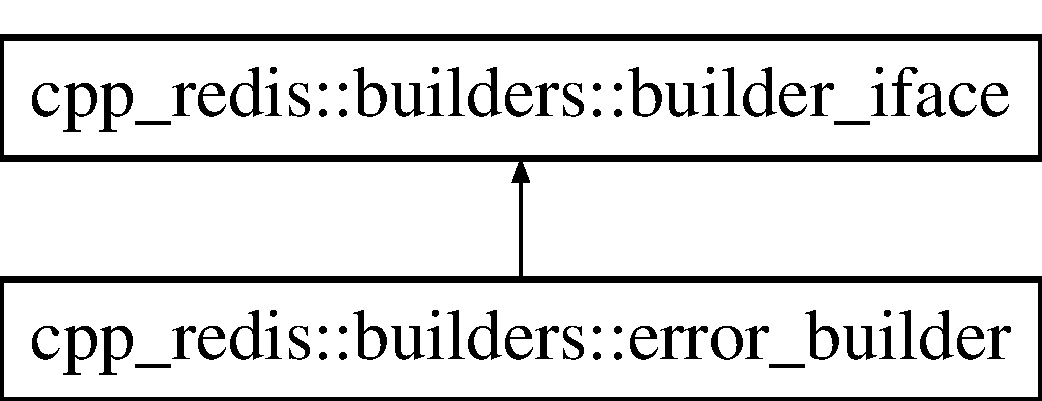
\includegraphics[height=2.000000cm]{classcpp__redis_1_1builders_1_1error__builder}
\end{center}
\end{figure}
\subsection*{Public Member Functions}
\begin{DoxyCompactItemize}
\item 
\mbox{\Hypertarget{classcpp__redis_1_1builders_1_1error__builder_abbc5e14b66702ec8b210fb1d288d2423}\label{classcpp__redis_1_1builders_1_1error__builder_abbc5e14b66702ec8b210fb1d288d2423}} 
\hyperlink{classcpp__redis_1_1builders_1_1error__builder_abbc5e14b66702ec8b210fb1d288d2423}{error\+\_\+builder} (void)=default
\begin{DoxyCompactList}\small\item\em ctor \end{DoxyCompactList}\item 
\mbox{\Hypertarget{classcpp__redis_1_1builders_1_1error__builder_a7650c178a457c57c2efb19e7ad256fe7}\label{classcpp__redis_1_1builders_1_1error__builder_a7650c178a457c57c2efb19e7ad256fe7}} 
\hyperlink{classcpp__redis_1_1builders_1_1error__builder_a7650c178a457c57c2efb19e7ad256fe7}{$\sim$error\+\_\+builder} (void)=default
\begin{DoxyCompactList}\small\item\em dtor \end{DoxyCompactList}\item 
\mbox{\Hypertarget{classcpp__redis_1_1builders_1_1error__builder_a2aee65fdc05abfacda73987e2cf60609}\label{classcpp__redis_1_1builders_1_1error__builder_a2aee65fdc05abfacda73987e2cf60609}} 
\hyperlink{classcpp__redis_1_1builders_1_1error__builder_a2aee65fdc05abfacda73987e2cf60609}{error\+\_\+builder} (const \hyperlink{classcpp__redis_1_1builders_1_1error__builder}{error\+\_\+builder} \&)=delete
\begin{DoxyCompactList}\small\item\em copy ctor \end{DoxyCompactList}\item 
\mbox{\Hypertarget{classcpp__redis_1_1builders_1_1error__builder_a0b1be51200ff84f17693ee888b03d505}\label{classcpp__redis_1_1builders_1_1error__builder_a0b1be51200ff84f17693ee888b03d505}} 
\hyperlink{classcpp__redis_1_1builders_1_1error__builder}{error\+\_\+builder} \& \hyperlink{classcpp__redis_1_1builders_1_1error__builder_a0b1be51200ff84f17693ee888b03d505}{operator=} (const \hyperlink{classcpp__redis_1_1builders_1_1error__builder}{error\+\_\+builder} \&)=delete
\begin{DoxyCompactList}\small\item\em assignment operator \end{DoxyCompactList}\item 
\hyperlink{classcpp__redis_1_1builders_1_1builder__iface}{builder\+\_\+iface} \& \hyperlink{classcpp__redis_1_1builders_1_1error__builder_af5ac542be148d6f8500de79fa3164798}{operator$<$$<$} (std\+::string \&data)
\item 
bool \hyperlink{classcpp__redis_1_1builders_1_1error__builder_af3d67647f012d0a7378684e2f8258a6d}{reply\+\_\+ready} (void) const
\item 
\hyperlink{classcpp__redis_1_1reply}{reply} \hyperlink{classcpp__redis_1_1builders_1_1error__builder_ae2b68b7daad4d71b6780e47bdcc1e32b}{get\+\_\+reply} (void) const
\item 
const std\+::string \& \hyperlink{classcpp__redis_1_1builders_1_1error__builder_adeef989fb2f5e47e001783cfda48e341}{get\+\_\+error} (void) const
\end{DoxyCompactItemize}


\subsection{Detailed Description}
builder to build redis error replies 

\subsection{Member Function Documentation}
\mbox{\Hypertarget{classcpp__redis_1_1builders_1_1error__builder_adeef989fb2f5e47e001783cfda48e341}\label{classcpp__redis_1_1builders_1_1error__builder_adeef989fb2f5e47e001783cfda48e341}} 
\index{cpp\+\_\+redis\+::builders\+::error\+\_\+builder@{cpp\+\_\+redis\+::builders\+::error\+\_\+builder}!get\+\_\+error@{get\+\_\+error}}
\index{get\+\_\+error@{get\+\_\+error}!cpp\+\_\+redis\+::builders\+::error\+\_\+builder@{cpp\+\_\+redis\+::builders\+::error\+\_\+builder}}
\subsubsection{\texorpdfstring{get\+\_\+error()}{get\_error()}}
{\footnotesize\ttfamily const std\+::string\& cpp\+\_\+redis\+::builders\+::error\+\_\+builder\+::get\+\_\+error (\begin{DoxyParamCaption}\item[{void}]{ }\end{DoxyParamCaption}) const}

\begin{DoxyReturn}{Returns}
the parsed error 
\end{DoxyReturn}
\mbox{\Hypertarget{classcpp__redis_1_1builders_1_1error__builder_ae2b68b7daad4d71b6780e47bdcc1e32b}\label{classcpp__redis_1_1builders_1_1error__builder_ae2b68b7daad4d71b6780e47bdcc1e32b}} 
\index{cpp\+\_\+redis\+::builders\+::error\+\_\+builder@{cpp\+\_\+redis\+::builders\+::error\+\_\+builder}!get\+\_\+reply@{get\+\_\+reply}}
\index{get\+\_\+reply@{get\+\_\+reply}!cpp\+\_\+redis\+::builders\+::error\+\_\+builder@{cpp\+\_\+redis\+::builders\+::error\+\_\+builder}}
\subsubsection{\texorpdfstring{get\+\_\+reply()}{get\_reply()}}
{\footnotesize\ttfamily \hyperlink{classcpp__redis_1_1reply}{reply} cpp\+\_\+redis\+::builders\+::error\+\_\+builder\+::get\+\_\+reply (\begin{DoxyParamCaption}\item[{void}]{ }\end{DoxyParamCaption}) const\hspace{0.3cm}{\ttfamily [virtual]}}

\begin{DoxyReturn}{Returns}
reply object 
\end{DoxyReturn}


Implements \hyperlink{classcpp__redis_1_1builders_1_1builder__iface_afd2ff2c2371c2a486116543b638b9413}{cpp\+\_\+redis\+::builders\+::builder\+\_\+iface}.

\mbox{\Hypertarget{classcpp__redis_1_1builders_1_1error__builder_af5ac542be148d6f8500de79fa3164798}\label{classcpp__redis_1_1builders_1_1error__builder_af5ac542be148d6f8500de79fa3164798}} 
\index{cpp\+\_\+redis\+::builders\+::error\+\_\+builder@{cpp\+\_\+redis\+::builders\+::error\+\_\+builder}!operator$<$$<$@{operator$<$$<$}}
\index{operator$<$$<$@{operator$<$$<$}!cpp\+\_\+redis\+::builders\+::error\+\_\+builder@{cpp\+\_\+redis\+::builders\+::error\+\_\+builder}}
\subsubsection{\texorpdfstring{operator$<$$<$()}{operator<<()}}
{\footnotesize\ttfamily \hyperlink{classcpp__redis_1_1builders_1_1builder__iface}{builder\+\_\+iface}\& cpp\+\_\+redis\+::builders\+::error\+\_\+builder\+::operator$<$$<$ (\begin{DoxyParamCaption}\item[{std\+::string \&}]{data }\end{DoxyParamCaption})\hspace{0.3cm}{\ttfamily [virtual]}}

take data as parameter which is consumed to build the reply every bytes used to build the reply must be removed from the buffer passed as parameter


\begin{DoxyParams}{Parameters}
{\em data} & data to be consumed \\
\hline
\end{DoxyParams}
\begin{DoxyReturn}{Returns}
current instance 
\end{DoxyReturn}


Implements \hyperlink{classcpp__redis_1_1builders_1_1builder__iface_a9892bbc9c887c31c2742dad4476e2fa6}{cpp\+\_\+redis\+::builders\+::builder\+\_\+iface}.

\mbox{\Hypertarget{classcpp__redis_1_1builders_1_1error__builder_af3d67647f012d0a7378684e2f8258a6d}\label{classcpp__redis_1_1builders_1_1error__builder_af3d67647f012d0a7378684e2f8258a6d}} 
\index{cpp\+\_\+redis\+::builders\+::error\+\_\+builder@{cpp\+\_\+redis\+::builders\+::error\+\_\+builder}!reply\+\_\+ready@{reply\+\_\+ready}}
\index{reply\+\_\+ready@{reply\+\_\+ready}!cpp\+\_\+redis\+::builders\+::error\+\_\+builder@{cpp\+\_\+redis\+::builders\+::error\+\_\+builder}}
\subsubsection{\texorpdfstring{reply\+\_\+ready()}{reply\_ready()}}
{\footnotesize\ttfamily bool cpp\+\_\+redis\+::builders\+::error\+\_\+builder\+::reply\+\_\+ready (\begin{DoxyParamCaption}\item[{void}]{ }\end{DoxyParamCaption}) const\hspace{0.3cm}{\ttfamily [virtual]}}

\begin{DoxyReturn}{Returns}
whether the reply could be built 
\end{DoxyReturn}


Implements \hyperlink{classcpp__redis_1_1builders_1_1builder__iface_a40db9a31d4ea1771777e74146d31e12d}{cpp\+\_\+redis\+::builders\+::builder\+\_\+iface}.



The documentation for this class was generated from the following file\+:\begin{DoxyCompactItemize}
\item 
includes/cpp\+\_\+redis/builders/error\+\_\+builder.\+hpp\end{DoxyCompactItemize}

\hypertarget{structcpp__redis_1_1helpers_1_1front}{}\section{cpp\+\_\+redis\+:\+:helpers\+:\+:front$<$ T, Ts $>$ Struct Template Reference}
\label{structcpp__redis_1_1helpers_1_1front}\index{cpp\+\_\+redis\+::helpers\+::front$<$ T, Ts $>$@{cpp\+\_\+redis\+::helpers\+::front$<$ T, Ts $>$}}


{\ttfamily \#include $<$variadic\+\_\+template.\+hpp$>$}

\subsection*{Public Types}
\begin{DoxyCompactItemize}
\item 
using \hyperlink{structcpp__redis_1_1helpers_1_1front_a23178392c9417cc5ada75205931d1768}{type} = T
\end{DoxyCompactItemize}


\subsection{Detailed Description}
\subsubsection*{template$<$typename T, typename... Ts$>$\newline
struct cpp\+\_\+redis\+::helpers\+::front$<$ T, Ts $>$}

type traits to return front element of a variadic list 

\subsection{Member Typedef Documentation}
\mbox{\Hypertarget{structcpp__redis_1_1helpers_1_1front_a23178392c9417cc5ada75205931d1768}\label{structcpp__redis_1_1helpers_1_1front_a23178392c9417cc5ada75205931d1768}} 
\index{cpp\+\_\+redis\+::helpers\+::front@{cpp\+\_\+redis\+::helpers\+::front}!type@{type}}
\index{type@{type}!cpp\+\_\+redis\+::helpers\+::front@{cpp\+\_\+redis\+::helpers\+::front}}
\subsubsection{\texorpdfstring{type}{type}}
{\footnotesize\ttfamily template$<$typename T , typename... Ts$>$ \\
using \hyperlink{structcpp__redis_1_1helpers_1_1front}{cpp\+\_\+redis\+::helpers\+::front}$<$ T, Ts $>$\+::\hyperlink{structcpp__redis_1_1helpers_1_1front_a23178392c9417cc5ada75205931d1768}{type} =  T}

front type of variadic list 

The documentation for this struct was generated from the following file\+:\begin{DoxyCompactItemize}
\item 
includes/cpp\+\_\+redis/helpers/variadic\+\_\+template.\+hpp\end{DoxyCompactItemize}

\hypertarget{classcpp__redis_1_1builders_1_1integer__builder}{}\section{cpp\+\_\+redis\+:\+:builders\+:\+:integer\+\_\+builder Class Reference}
\label{classcpp__redis_1_1builders_1_1integer__builder}\index{cpp\+\_\+redis\+::builders\+::integer\+\_\+builder@{cpp\+\_\+redis\+::builders\+::integer\+\_\+builder}}


{\ttfamily \#include $<$integer\+\_\+builder.\+hpp$>$}

Inheritance diagram for cpp\+\_\+redis\+:\+:builders\+:\+:integer\+\_\+builder\+:\begin{figure}[H]
\begin{center}
\leavevmode
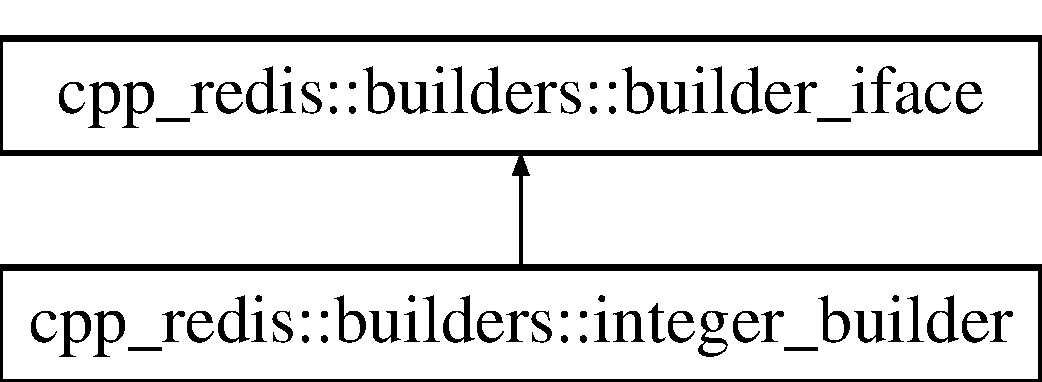
\includegraphics[height=2.000000cm]{classcpp__redis_1_1builders_1_1integer__builder}
\end{center}
\end{figure}
\subsection*{Public Member Functions}
\begin{DoxyCompactItemize}
\item 
\mbox{\Hypertarget{classcpp__redis_1_1builders_1_1integer__builder_a9ff2d3d27da0fb8b98fc4a0ea255fece}\label{classcpp__redis_1_1builders_1_1integer__builder_a9ff2d3d27da0fb8b98fc4a0ea255fece}} 
\hyperlink{classcpp__redis_1_1builders_1_1integer__builder_a9ff2d3d27da0fb8b98fc4a0ea255fece}{integer\+\_\+builder} (void)
\begin{DoxyCompactList}\small\item\em ctor \end{DoxyCompactList}\item 
\mbox{\Hypertarget{classcpp__redis_1_1builders_1_1integer__builder_ab2b797dd89b1bdec50f8ccf07633162f}\label{classcpp__redis_1_1builders_1_1integer__builder_ab2b797dd89b1bdec50f8ccf07633162f}} 
\hyperlink{classcpp__redis_1_1builders_1_1integer__builder_ab2b797dd89b1bdec50f8ccf07633162f}{$\sim$integer\+\_\+builder} (void)=default
\begin{DoxyCompactList}\small\item\em dtor \end{DoxyCompactList}\item 
\mbox{\Hypertarget{classcpp__redis_1_1builders_1_1integer__builder_ab451b7fe5de8cf6f618cf9be1569aa41}\label{classcpp__redis_1_1builders_1_1integer__builder_ab451b7fe5de8cf6f618cf9be1569aa41}} 
\hyperlink{classcpp__redis_1_1builders_1_1integer__builder_ab451b7fe5de8cf6f618cf9be1569aa41}{integer\+\_\+builder} (const \hyperlink{classcpp__redis_1_1builders_1_1integer__builder}{integer\+\_\+builder} \&)=delete
\begin{DoxyCompactList}\small\item\em copy ctor \end{DoxyCompactList}\item 
\mbox{\Hypertarget{classcpp__redis_1_1builders_1_1integer__builder_a259905e8a34765d6ff9d2dd64f444b54}\label{classcpp__redis_1_1builders_1_1integer__builder_a259905e8a34765d6ff9d2dd64f444b54}} 
\hyperlink{classcpp__redis_1_1builders_1_1integer__builder}{integer\+\_\+builder} \& \hyperlink{classcpp__redis_1_1builders_1_1integer__builder_a259905e8a34765d6ff9d2dd64f444b54}{operator=} (const \hyperlink{classcpp__redis_1_1builders_1_1integer__builder}{integer\+\_\+builder} \&)=delete
\begin{DoxyCompactList}\small\item\em assignment operator \end{DoxyCompactList}\item 
\hyperlink{classcpp__redis_1_1builders_1_1builder__iface}{builder\+\_\+iface} \& \hyperlink{classcpp__redis_1_1builders_1_1integer__builder_ae29f074134f7269db7f947b0fcbe312e}{operator$<$$<$} (std\+::string \&data)
\item 
bool \hyperlink{classcpp__redis_1_1builders_1_1integer__builder_a4893dc36d06d75094bb4fe3fbc826966}{reply\+\_\+ready} (void) const
\item 
\hyperlink{classcpp__redis_1_1reply}{reply} \hyperlink{classcpp__redis_1_1builders_1_1integer__builder_a25221763ba6f8b740458c673945208e0}{get\+\_\+reply} (void) const
\item 
int64\+\_\+t \hyperlink{classcpp__redis_1_1builders_1_1integer__builder_af68431c4c81242c1930b3b4feb2028e5}{get\+\_\+integer} (void) const
\end{DoxyCompactItemize}


\subsection{Detailed Description}
builder to build redis integer replies 

\subsection{Member Function Documentation}
\mbox{\Hypertarget{classcpp__redis_1_1builders_1_1integer__builder_af68431c4c81242c1930b3b4feb2028e5}\label{classcpp__redis_1_1builders_1_1integer__builder_af68431c4c81242c1930b3b4feb2028e5}} 
\index{cpp\+\_\+redis\+::builders\+::integer\+\_\+builder@{cpp\+\_\+redis\+::builders\+::integer\+\_\+builder}!get\+\_\+integer@{get\+\_\+integer}}
\index{get\+\_\+integer@{get\+\_\+integer}!cpp\+\_\+redis\+::builders\+::integer\+\_\+builder@{cpp\+\_\+redis\+::builders\+::integer\+\_\+builder}}
\subsubsection{\texorpdfstring{get\+\_\+integer()}{get\_integer()}}
{\footnotesize\ttfamily int64\+\_\+t cpp\+\_\+redis\+::builders\+::integer\+\_\+builder\+::get\+\_\+integer (\begin{DoxyParamCaption}\item[{void}]{ }\end{DoxyParamCaption}) const}

\begin{DoxyReturn}{Returns}
the parsed integer 
\end{DoxyReturn}
\mbox{\Hypertarget{classcpp__redis_1_1builders_1_1integer__builder_a25221763ba6f8b740458c673945208e0}\label{classcpp__redis_1_1builders_1_1integer__builder_a25221763ba6f8b740458c673945208e0}} 
\index{cpp\+\_\+redis\+::builders\+::integer\+\_\+builder@{cpp\+\_\+redis\+::builders\+::integer\+\_\+builder}!get\+\_\+reply@{get\+\_\+reply}}
\index{get\+\_\+reply@{get\+\_\+reply}!cpp\+\_\+redis\+::builders\+::integer\+\_\+builder@{cpp\+\_\+redis\+::builders\+::integer\+\_\+builder}}
\subsubsection{\texorpdfstring{get\+\_\+reply()}{get\_reply()}}
{\footnotesize\ttfamily \hyperlink{classcpp__redis_1_1reply}{reply} cpp\+\_\+redis\+::builders\+::integer\+\_\+builder\+::get\+\_\+reply (\begin{DoxyParamCaption}\item[{void}]{ }\end{DoxyParamCaption}) const\hspace{0.3cm}{\ttfamily [virtual]}}

\begin{DoxyReturn}{Returns}
reply object 
\end{DoxyReturn}


Implements \hyperlink{classcpp__redis_1_1builders_1_1builder__iface_afd2ff2c2371c2a486116543b638b9413}{cpp\+\_\+redis\+::builders\+::builder\+\_\+iface}.

\mbox{\Hypertarget{classcpp__redis_1_1builders_1_1integer__builder_ae29f074134f7269db7f947b0fcbe312e}\label{classcpp__redis_1_1builders_1_1integer__builder_ae29f074134f7269db7f947b0fcbe312e}} 
\index{cpp\+\_\+redis\+::builders\+::integer\+\_\+builder@{cpp\+\_\+redis\+::builders\+::integer\+\_\+builder}!operator$<$$<$@{operator$<$$<$}}
\index{operator$<$$<$@{operator$<$$<$}!cpp\+\_\+redis\+::builders\+::integer\+\_\+builder@{cpp\+\_\+redis\+::builders\+::integer\+\_\+builder}}
\subsubsection{\texorpdfstring{operator$<$$<$()}{operator<<()}}
{\footnotesize\ttfamily \hyperlink{classcpp__redis_1_1builders_1_1builder__iface}{builder\+\_\+iface}\& cpp\+\_\+redis\+::builders\+::integer\+\_\+builder\+::operator$<$$<$ (\begin{DoxyParamCaption}\item[{std\+::string \&}]{data }\end{DoxyParamCaption})\hspace{0.3cm}{\ttfamily [virtual]}}

take data as parameter which is consumed to build the reply every bytes used to build the reply must be removed from the buffer passed as parameter


\begin{DoxyParams}{Parameters}
{\em data} & data to be consumed \\
\hline
\end{DoxyParams}
\begin{DoxyReturn}{Returns}
current instance 
\end{DoxyReturn}


Implements \hyperlink{classcpp__redis_1_1builders_1_1builder__iface_a9892bbc9c887c31c2742dad4476e2fa6}{cpp\+\_\+redis\+::builders\+::builder\+\_\+iface}.

\mbox{\Hypertarget{classcpp__redis_1_1builders_1_1integer__builder_a4893dc36d06d75094bb4fe3fbc826966}\label{classcpp__redis_1_1builders_1_1integer__builder_a4893dc36d06d75094bb4fe3fbc826966}} 
\index{cpp\+\_\+redis\+::builders\+::integer\+\_\+builder@{cpp\+\_\+redis\+::builders\+::integer\+\_\+builder}!reply\+\_\+ready@{reply\+\_\+ready}}
\index{reply\+\_\+ready@{reply\+\_\+ready}!cpp\+\_\+redis\+::builders\+::integer\+\_\+builder@{cpp\+\_\+redis\+::builders\+::integer\+\_\+builder}}
\subsubsection{\texorpdfstring{reply\+\_\+ready()}{reply\_ready()}}
{\footnotesize\ttfamily bool cpp\+\_\+redis\+::builders\+::integer\+\_\+builder\+::reply\+\_\+ready (\begin{DoxyParamCaption}\item[{void}]{ }\end{DoxyParamCaption}) const\hspace{0.3cm}{\ttfamily [virtual]}}

\begin{DoxyReturn}{Returns}
whether the reply could be built 
\end{DoxyReturn}


Implements \hyperlink{classcpp__redis_1_1builders_1_1builder__iface_a40db9a31d4ea1771777e74146d31e12d}{cpp\+\_\+redis\+::builders\+::builder\+\_\+iface}.



The documentation for this class was generated from the following file\+:\begin{DoxyCompactItemize}
\item 
includes/cpp\+\_\+redis/builders/integer\+\_\+builder.\+hpp\end{DoxyCompactItemize}

\hypertarget{structcpp__redis_1_1helpers_1_1is__different__types}{}\section{cpp\+\_\+redis\+:\+:helpers\+:\+:is\+\_\+different\+\_\+types$<$ T, Args $>$ Struct Template Reference}
\label{structcpp__redis_1_1helpers_1_1is__different__types}\index{cpp\+\_\+redis\+::helpers\+::is\+\_\+different\+\_\+types$<$ T, Args $>$@{cpp\+\_\+redis\+::helpers\+::is\+\_\+different\+\_\+types$<$ T, Args $>$}}


{\ttfamily \#include $<$variadic\+\_\+template.\+hpp$>$}

\subsection*{Static Public Attributes}
\begin{DoxyCompactItemize}
\item 
static constexpr bool \hyperlink{structcpp__redis_1_1helpers_1_1is__different__types_a07dadd8ff3c8024734f231aaf1555626}{value}
\end{DoxyCompactItemize}


\subsection{Detailed Description}
\subsubsection*{template$<$typename T, typename... Args$>$\newline
struct cpp\+\_\+redis\+::helpers\+::is\+\_\+different\+\_\+types$<$ T, Args $>$}

type traits to check if type is not present in variadic list 

\subsection{Member Data Documentation}
\mbox{\Hypertarget{structcpp__redis_1_1helpers_1_1is__different__types_a07dadd8ff3c8024734f231aaf1555626}\label{structcpp__redis_1_1helpers_1_1is__different__types_a07dadd8ff3c8024734f231aaf1555626}} 
\index{cpp\+\_\+redis\+::helpers\+::is\+\_\+different\+\_\+types@{cpp\+\_\+redis\+::helpers\+::is\+\_\+different\+\_\+types}!value@{value}}
\index{value@{value}!cpp\+\_\+redis\+::helpers\+::is\+\_\+different\+\_\+types@{cpp\+\_\+redis\+::helpers\+::is\+\_\+different\+\_\+types}}
\subsubsection{\texorpdfstring{value}{value}}
{\footnotesize\ttfamily template$<$typename T , typename... Args$>$ \\
constexpr bool \hyperlink{structcpp__redis_1_1helpers_1_1is__different__types}{cpp\+\_\+redis\+::helpers\+::is\+\_\+different\+\_\+types}$<$ T, Args $>$\+::value\hspace{0.3cm}{\ttfamily [static]}}

{\bfseries Initial value\+:}
\begin{DoxyCode}
= is\_type\_present<T, Args...>\hyperlink{structcpp__redis_1_1helpers_1_1is__different__types_a07dadd8ff3c8024734f231aaf1555626}{::value}
                                  ? false
                                  : is\_different\_types<Args...>\hyperlink{structcpp__redis_1_1helpers_1_1is__different__types_a07dadd8ff3c8024734f231aaf1555626}{::value}
\end{DoxyCode}


The documentation for this struct was generated from the following file\+:\begin{DoxyCompactItemize}
\item 
includes/cpp\+\_\+redis/helpers/\hyperlink{variadic__template_8hpp}{variadic\+\_\+template.\+hpp}\end{DoxyCompactItemize}

\hypertarget{structcpp__redis_1_1helpers_1_1is__different__types_3_01_t1_01_4}{}\section{cpp\+\_\+redis\+:\+:helpers\+:\+:is\+\_\+different\+\_\+types$<$ T1 $>$ Struct Template Reference}
\label{structcpp__redis_1_1helpers_1_1is__different__types_3_01_t1_01_4}\index{cpp\+\_\+redis\+::helpers\+::is\+\_\+different\+\_\+types$<$ T1 $>$@{cpp\+\_\+redis\+::helpers\+::is\+\_\+different\+\_\+types$<$ T1 $>$}}


{\ttfamily \#include $<$variadic\+\_\+template.\+hpp$>$}

\subsection*{Static Public Attributes}
\begin{DoxyCompactItemize}
\item 
static constexpr bool \hyperlink{structcpp__redis_1_1helpers_1_1is__different__types_3_01_t1_01_4_ae05b9b4af6846340ac66fcf64a622397}{value} = true
\end{DoxyCompactItemize}


\subsection{Detailed Description}
\subsubsection*{template$<$typename T1$>$\newline
struct cpp\+\_\+redis\+::helpers\+::is\+\_\+different\+\_\+types$<$ T1 $>$}

type traits to check if type is not present in variadic list 

\subsection{Member Data Documentation}
\mbox{\Hypertarget{structcpp__redis_1_1helpers_1_1is__different__types_3_01_t1_01_4_ae05b9b4af6846340ac66fcf64a622397}\label{structcpp__redis_1_1helpers_1_1is__different__types_3_01_t1_01_4_ae05b9b4af6846340ac66fcf64a622397}} 
\index{cpp\+\_\+redis\+::helpers\+::is\+\_\+different\+\_\+types$<$ T1 $>$@{cpp\+\_\+redis\+::helpers\+::is\+\_\+different\+\_\+types$<$ T1 $>$}!value@{value}}
\index{value@{value}!cpp\+\_\+redis\+::helpers\+::is\+\_\+different\+\_\+types$<$ T1 $>$@{cpp\+\_\+redis\+::helpers\+::is\+\_\+different\+\_\+types$<$ T1 $>$}}
\subsubsection{\texorpdfstring{value}{value}}
{\footnotesize\ttfamily template$<$typename T1 $>$ \\
constexpr bool \hyperlink{structcpp__redis_1_1helpers_1_1is__different__types}{cpp\+\_\+redis\+::helpers\+::is\+\_\+different\+\_\+types}$<$ T1 $>$\+::value = true\hspace{0.3cm}{\ttfamily [static]}}



The documentation for this struct was generated from the following file\+:\begin{DoxyCompactItemize}
\item 
includes/cpp\+\_\+redis/helpers/\hyperlink{variadic__template_8hpp}{variadic\+\_\+template.\+hpp}\end{DoxyCompactItemize}

\hypertarget{structcpp__redis_1_1helpers_1_1is__type__present}{}\section{cpp\+\_\+redis\+:\+:helpers\+:\+:is\+\_\+type\+\_\+present$<$ T1, T2, Ts $>$ Struct Template Reference}
\label{structcpp__redis_1_1helpers_1_1is__type__present}\index{cpp\+\_\+redis\+::helpers\+::is\+\_\+type\+\_\+present$<$ T1, T2, Ts $>$@{cpp\+\_\+redis\+::helpers\+::is\+\_\+type\+\_\+present$<$ T1, T2, Ts $>$}}


{\ttfamily \#include $<$variadic\+\_\+template.\+hpp$>$}

\subsection*{Static Public Attributes}
\begin{DoxyCompactItemize}
\item 
static constexpr bool \hyperlink{structcpp__redis_1_1helpers_1_1is__type__present_a7b5e8d970ba974a9b58cbc440983c25c}{value}
\end{DoxyCompactItemize}


\subsection{Detailed Description}
\subsubsection*{template$<$typename T1, typename T2, typename... Ts$>$\newline
struct cpp\+\_\+redis\+::helpers\+::is\+\_\+type\+\_\+present$<$ T1, T2, Ts $>$}

type traits to check if type is present in variadic list 

\subsection{Member Data Documentation}
\mbox{\Hypertarget{structcpp__redis_1_1helpers_1_1is__type__present_a7b5e8d970ba974a9b58cbc440983c25c}\label{structcpp__redis_1_1helpers_1_1is__type__present_a7b5e8d970ba974a9b58cbc440983c25c}} 
\index{cpp\+\_\+redis\+::helpers\+::is\+\_\+type\+\_\+present@{cpp\+\_\+redis\+::helpers\+::is\+\_\+type\+\_\+present}!value@{value}}
\index{value@{value}!cpp\+\_\+redis\+::helpers\+::is\+\_\+type\+\_\+present@{cpp\+\_\+redis\+::helpers\+::is\+\_\+type\+\_\+present}}
\subsubsection{\texorpdfstring{value}{value}}
{\footnotesize\ttfamily template$<$typename T1 , typename T2 , typename... Ts$>$ \\
constexpr bool \hyperlink{structcpp__redis_1_1helpers_1_1is__type__present}{cpp\+\_\+redis\+::helpers\+::is\+\_\+type\+\_\+present}$<$ T1, T2, Ts $>$\+::value\hspace{0.3cm}{\ttfamily [static]}}

{\bfseries Initial value\+:}
\begin{DoxyCode}
= std::is\_same<T1, T2>::value
                                  ? true
                                  : is\_type\_present<T1, Ts...>\hyperlink{structcpp__redis_1_1helpers_1_1is__type__present_a7b5e8d970ba974a9b58cbc440983c25c}{::value}
\end{DoxyCode}


The documentation for this struct was generated from the following file\+:\begin{DoxyCompactItemize}
\item 
includes/cpp\+\_\+redis/helpers/\hyperlink{variadic__template_8hpp}{variadic\+\_\+template.\+hpp}\end{DoxyCompactItemize}

\hypertarget{structcpp__redis_1_1helpers_1_1is__type__present_3_01_t1_00_01_t2_01_4}{}\section{cpp\+\_\+redis\+:\+:helpers\+:\+:is\+\_\+type\+\_\+present$<$ T1, T2 $>$ Struct Template Reference}
\label{structcpp__redis_1_1helpers_1_1is__type__present_3_01_t1_00_01_t2_01_4}\index{cpp\+\_\+redis\+::helpers\+::is\+\_\+type\+\_\+present$<$ T1, T2 $>$@{cpp\+\_\+redis\+::helpers\+::is\+\_\+type\+\_\+present$<$ T1, T2 $>$}}


{\ttfamily \#include $<$variadic\+\_\+template.\+hpp$>$}

\subsection*{Static Public Attributes}
\begin{DoxyCompactItemize}
\item 
static constexpr bool \hyperlink{structcpp__redis_1_1helpers_1_1is__type__present_3_01_t1_00_01_t2_01_4_a1dbf43b76ba407caf9bfb35ffdbe55ad}{value} = std\+::is\+\_\+same$<$T1, T2$>$\+::value
\end{DoxyCompactItemize}


\subsection{Detailed Description}
\subsubsection*{template$<$typename T1, typename T2$>$\newline
struct cpp\+\_\+redis\+::helpers\+::is\+\_\+type\+\_\+present$<$ T1, T2 $>$}

type traits to check if type is present in variadic list 

\subsection{Member Data Documentation}
\mbox{\Hypertarget{structcpp__redis_1_1helpers_1_1is__type__present_3_01_t1_00_01_t2_01_4_a1dbf43b76ba407caf9bfb35ffdbe55ad}\label{structcpp__redis_1_1helpers_1_1is__type__present_3_01_t1_00_01_t2_01_4_a1dbf43b76ba407caf9bfb35ffdbe55ad}} 
\index{cpp\+\_\+redis\+::helpers\+::is\+\_\+type\+\_\+present$<$ T1, T2 $>$@{cpp\+\_\+redis\+::helpers\+::is\+\_\+type\+\_\+present$<$ T1, T2 $>$}!value@{value}}
\index{value@{value}!cpp\+\_\+redis\+::helpers\+::is\+\_\+type\+\_\+present$<$ T1, T2 $>$@{cpp\+\_\+redis\+::helpers\+::is\+\_\+type\+\_\+present$<$ T1, T2 $>$}}
\subsubsection{\texorpdfstring{value}{value}}
{\footnotesize\ttfamily template$<$typename T1 , typename T2 $>$ \\
constexpr bool \hyperlink{structcpp__redis_1_1helpers_1_1is__type__present}{cpp\+\_\+redis\+::helpers\+::is\+\_\+type\+\_\+present}$<$ T1, T2 $>$\+::value = std\+::is\+\_\+same$<$T1, T2$>$\+::value\hspace{0.3cm}{\ttfamily [static]}}

true if T1 and T2 are the same false otherwise 

The documentation for this struct was generated from the following file\+:\begin{DoxyCompactItemize}
\item 
includes/cpp\+\_\+redis/helpers/variadic\+\_\+template.\+hpp\end{DoxyCompactItemize}

\hypertarget{classcpp__redis_1_1logger}{}\section{cpp\+\_\+redis\+:\+:logger Class Reference}
\label{classcpp__redis_1_1logger}\index{cpp\+\_\+redis\+::logger@{cpp\+\_\+redis\+::logger}}


{\ttfamily \#include $<$logger.\+hpp$>$}

Inheritance diagram for cpp\+\_\+redis\+:\+:logger\+:\begin{figure}[H]
\begin{center}
\leavevmode
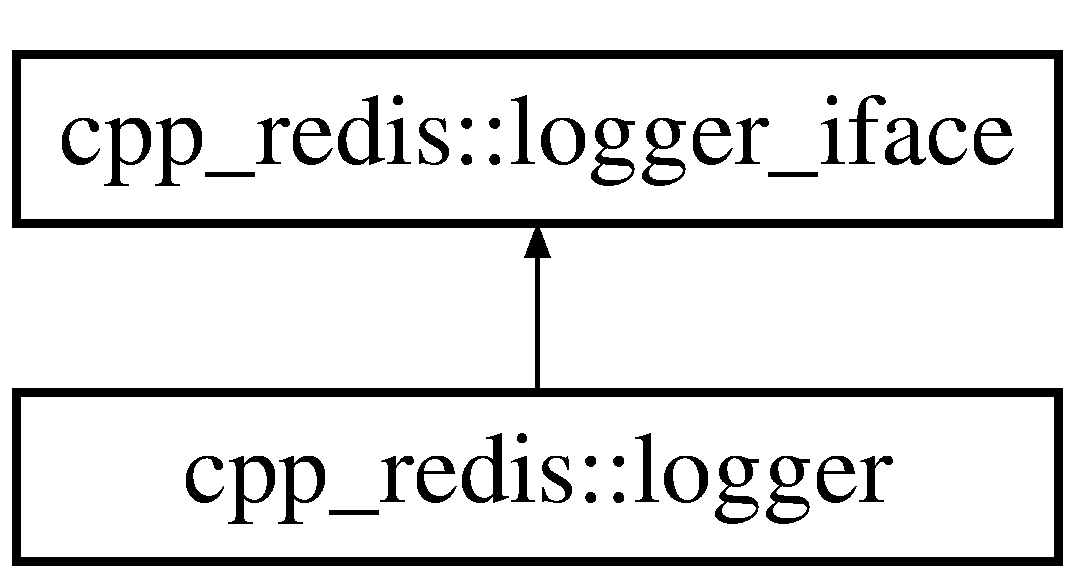
\includegraphics[height=2.000000cm]{classcpp__redis_1_1logger}
\end{center}
\end{figure}
\subsection*{Public Types}
\begin{DoxyCompactItemize}
\item 
enum \hyperlink{classcpp__redis_1_1logger_a9493594d547e7abe71b8690be1946c7a}{log\+\_\+level} \{ \hyperlink{classcpp__redis_1_1logger_a9493594d547e7abe71b8690be1946c7aacb5e100e5a9a3e7f6d1fd97512215282}{log\+\_\+level\+::error} = 0, 
\hyperlink{classcpp__redis_1_1logger_a9493594d547e7abe71b8690be1946c7aa1ea4c3ab05ee0c6d4de30740443769cb}{log\+\_\+level\+::warn} = 1, 
\hyperlink{classcpp__redis_1_1logger_a9493594d547e7abe71b8690be1946c7aacaf9b6b99962bf5c2264824231d7a40c}{log\+\_\+level\+::info} = 2, 
\hyperlink{classcpp__redis_1_1logger_a9493594d547e7abe71b8690be1946c7aaad42f6697b035b7580e4fef93be20b4d}{log\+\_\+level\+::debug} = 3
 \}
\end{DoxyCompactItemize}
\subsection*{Public Member Functions}
\begin{DoxyCompactItemize}
\item 
\hyperlink{classcpp__redis_1_1logger_a36b15a75690a087fca7d304852785512}{logger} (\hyperlink{classcpp__redis_1_1logger_a9493594d547e7abe71b8690be1946c7a}{log\+\_\+level} level=\hyperlink{classcpp__redis_1_1logger_a9493594d547e7abe71b8690be1946c7aacaf9b6b99962bf5c2264824231d7a40c}{log\+\_\+level\+::info})
\begin{DoxyCompactList}\small\item\em ctor \end{DoxyCompactList}\item 
\hyperlink{classcpp__redis_1_1logger_ab5eb02b26c96a6e5cba9a7d30669f625}{$\sim$logger} (void)=default
\begin{DoxyCompactList}\small\item\em dtor \end{DoxyCompactList}\item 
\hyperlink{classcpp__redis_1_1logger_aec0854d47a13f91e09db25e745a3d722}{logger} (const \hyperlink{classcpp__redis_1_1logger}{logger} \&)=default
\begin{DoxyCompactList}\small\item\em copy ctor \end{DoxyCompactList}\item 
\hyperlink{classcpp__redis_1_1logger}{logger} \& \hyperlink{classcpp__redis_1_1logger_a09d012d32f35421a16ec73143adc4415}{operator=} (const \hyperlink{classcpp__redis_1_1logger}{logger} \&)=default
\begin{DoxyCompactList}\small\item\em assignment operator \end{DoxyCompactList}\item 
void \hyperlink{classcpp__redis_1_1logger_a36e0908e7b05850b663a4b8b9cdbc299}{debug} (const std\+::string \&msg, const std\+::string \&file, std\+::size\+\_\+t line)
\item 
void \hyperlink{classcpp__redis_1_1logger_a04c741b5110946e76bb23728da6fb2ac}{info} (const std\+::string \&msg, const std\+::string \&file, std\+::size\+\_\+t line)
\item 
void \hyperlink{classcpp__redis_1_1logger_ae9359429428786c7b5605a1109508ae5}{warn} (const std\+::string \&msg, const std\+::string \&file, std\+::size\+\_\+t line)
\item 
void \hyperlink{classcpp__redis_1_1logger_aaf7f2837511f4414a4d7b7b923ebc15e}{error} (const std\+::string \&msg, const std\+::string \&file, std\+::size\+\_\+t line)
\end{DoxyCompactItemize}
\subsection*{Private Attributes}
\begin{DoxyCompactItemize}
\item 
\hyperlink{classcpp__redis_1_1logger_a9493594d547e7abe71b8690be1946c7a}{log\+\_\+level} \hyperlink{classcpp__redis_1_1logger_af9f41a47abdc48c69cf35a41c14f7a52}{m\+\_\+level}
\item 
std\+::mutex \hyperlink{classcpp__redis_1_1logger_a74810c30886b21bde6590c0d21234c05}{m\+\_\+mutex}
\end{DoxyCompactItemize}


\subsection{Detailed Description}
default logger class provided by the library 

\subsection{Member Enumeration Documentation}
\mbox{\Hypertarget{classcpp__redis_1_1logger_a9493594d547e7abe71b8690be1946c7a}\label{classcpp__redis_1_1logger_a9493594d547e7abe71b8690be1946c7a}} 
\index{cpp\+\_\+redis\+::logger@{cpp\+\_\+redis\+::logger}!log\+\_\+level@{log\+\_\+level}}
\index{log\+\_\+level@{log\+\_\+level}!cpp\+\_\+redis\+::logger@{cpp\+\_\+redis\+::logger}}
\subsubsection{\texorpdfstring{log\+\_\+level}{log\_level}}
{\footnotesize\ttfamily enum \hyperlink{classcpp__redis_1_1logger_a9493594d547e7abe71b8690be1946c7a}{cpp\+\_\+redis\+::logger\+::log\+\_\+level}\hspace{0.3cm}{\ttfamily [strong]}}

log level \begin{DoxyEnumFields}{Enumerator}
\raisebox{\heightof{T}}[0pt][0pt]{\index{error@{error}!cpp\+\_\+redis\+::logger@{cpp\+\_\+redis\+::logger}}\index{cpp\+\_\+redis\+::logger@{cpp\+\_\+redis\+::logger}!error@{error}}}\mbox{\Hypertarget{classcpp__redis_1_1logger_a9493594d547e7abe71b8690be1946c7aacb5e100e5a9a3e7f6d1fd97512215282}\label{classcpp__redis_1_1logger_a9493594d547e7abe71b8690be1946c7aacb5e100e5a9a3e7f6d1fd97512215282}} 
error&\\
\hline

\raisebox{\heightof{T}}[0pt][0pt]{\index{warn@{warn}!cpp\+\_\+redis\+::logger@{cpp\+\_\+redis\+::logger}}\index{cpp\+\_\+redis\+::logger@{cpp\+\_\+redis\+::logger}!warn@{warn}}}\mbox{\Hypertarget{classcpp__redis_1_1logger_a9493594d547e7abe71b8690be1946c7aa1ea4c3ab05ee0c6d4de30740443769cb}\label{classcpp__redis_1_1logger_a9493594d547e7abe71b8690be1946c7aa1ea4c3ab05ee0c6d4de30740443769cb}} 
warn&\\
\hline

\raisebox{\heightof{T}}[0pt][0pt]{\index{info@{info}!cpp\+\_\+redis\+::logger@{cpp\+\_\+redis\+::logger}}\index{cpp\+\_\+redis\+::logger@{cpp\+\_\+redis\+::logger}!info@{info}}}\mbox{\Hypertarget{classcpp__redis_1_1logger_a9493594d547e7abe71b8690be1946c7aacaf9b6b99962bf5c2264824231d7a40c}\label{classcpp__redis_1_1logger_a9493594d547e7abe71b8690be1946c7aacaf9b6b99962bf5c2264824231d7a40c}} 
info&\\
\hline

\raisebox{\heightof{T}}[0pt][0pt]{\index{debug@{debug}!cpp\+\_\+redis\+::logger@{cpp\+\_\+redis\+::logger}}\index{cpp\+\_\+redis\+::logger@{cpp\+\_\+redis\+::logger}!debug@{debug}}}\mbox{\Hypertarget{classcpp__redis_1_1logger_a9493594d547e7abe71b8690be1946c7aaad42f6697b035b7580e4fef93be20b4d}\label{classcpp__redis_1_1logger_a9493594d547e7abe71b8690be1946c7aaad42f6697b035b7580e4fef93be20b4d}} 
debug&\\
\hline

\end{DoxyEnumFields}


\subsection{Constructor \& Destructor Documentation}
\mbox{\Hypertarget{classcpp__redis_1_1logger_a36b15a75690a087fca7d304852785512}\label{classcpp__redis_1_1logger_a36b15a75690a087fca7d304852785512}} 
\index{cpp\+\_\+redis\+::logger@{cpp\+\_\+redis\+::logger}!logger@{logger}}
\index{logger@{logger}!cpp\+\_\+redis\+::logger@{cpp\+\_\+redis\+::logger}}
\subsubsection{\texorpdfstring{logger()}{logger()}\hspace{0.1cm}{\footnotesize\ttfamily [1/2]}}
{\footnotesize\ttfamily cpp\+\_\+redis\+::logger\+::logger (\begin{DoxyParamCaption}\item[{\hyperlink{classcpp__redis_1_1logger_a9493594d547e7abe71b8690be1946c7a}{log\+\_\+level}}]{level = {\ttfamily \hyperlink{classcpp__redis_1_1logger_a9493594d547e7abe71b8690be1946c7aacaf9b6b99962bf5c2264824231d7a40c}{log\+\_\+level\+::info}} }\end{DoxyParamCaption})}



ctor 

\mbox{\Hypertarget{classcpp__redis_1_1logger_ab5eb02b26c96a6e5cba9a7d30669f625}\label{classcpp__redis_1_1logger_ab5eb02b26c96a6e5cba9a7d30669f625}} 
\index{cpp\+\_\+redis\+::logger@{cpp\+\_\+redis\+::logger}!````~logger@{$\sim$logger}}
\index{````~logger@{$\sim$logger}!cpp\+\_\+redis\+::logger@{cpp\+\_\+redis\+::logger}}
\subsubsection{\texorpdfstring{$\sim$logger()}{~logger()}}
{\footnotesize\ttfamily cpp\+\_\+redis\+::logger\+::$\sim$logger (\begin{DoxyParamCaption}\item[{void}]{ }\end{DoxyParamCaption})\hspace{0.3cm}{\ttfamily [default]}}



dtor 

\mbox{\Hypertarget{classcpp__redis_1_1logger_aec0854d47a13f91e09db25e745a3d722}\label{classcpp__redis_1_1logger_aec0854d47a13f91e09db25e745a3d722}} 
\index{cpp\+\_\+redis\+::logger@{cpp\+\_\+redis\+::logger}!logger@{logger}}
\index{logger@{logger}!cpp\+\_\+redis\+::logger@{cpp\+\_\+redis\+::logger}}
\subsubsection{\texorpdfstring{logger()}{logger()}\hspace{0.1cm}{\footnotesize\ttfamily [2/2]}}
{\footnotesize\ttfamily cpp\+\_\+redis\+::logger\+::logger (\begin{DoxyParamCaption}\item[{const \hyperlink{classcpp__redis_1_1logger}{logger} \&}]{ }\end{DoxyParamCaption})\hspace{0.3cm}{\ttfamily [default]}}



copy ctor 



\subsection{Member Function Documentation}
\mbox{\Hypertarget{classcpp__redis_1_1logger_a36e0908e7b05850b663a4b8b9cdbc299}\label{classcpp__redis_1_1logger_a36e0908e7b05850b663a4b8b9cdbc299}} 
\index{cpp\+\_\+redis\+::logger@{cpp\+\_\+redis\+::logger}!debug@{debug}}
\index{debug@{debug}!cpp\+\_\+redis\+::logger@{cpp\+\_\+redis\+::logger}}
\subsubsection{\texorpdfstring{debug()}{debug()}}
{\footnotesize\ttfamily void cpp\+\_\+redis\+::logger\+::debug (\begin{DoxyParamCaption}\item[{const std\+::string \&}]{msg,  }\item[{const std\+::string \&}]{file,  }\item[{std\+::size\+\_\+t}]{line }\end{DoxyParamCaption})\hspace{0.3cm}{\ttfamily [virtual]}}

debug logging


\begin{DoxyParams}{Parameters}
{\em msg} & message to be logged \\
\hline
{\em file} & file from which the message is coming \\
\hline
{\em line} & line in the file of the message \\
\hline
\end{DoxyParams}


Implements \hyperlink{classcpp__redis_1_1logger__iface_aaace9e12cbb32d7bdd76c17180a30de7}{cpp\+\_\+redis\+::logger\+\_\+iface}.

\mbox{\Hypertarget{classcpp__redis_1_1logger_aaf7f2837511f4414a4d7b7b923ebc15e}\label{classcpp__redis_1_1logger_aaf7f2837511f4414a4d7b7b923ebc15e}} 
\index{cpp\+\_\+redis\+::logger@{cpp\+\_\+redis\+::logger}!error@{error}}
\index{error@{error}!cpp\+\_\+redis\+::logger@{cpp\+\_\+redis\+::logger}}
\subsubsection{\texorpdfstring{error()}{error()}}
{\footnotesize\ttfamily void cpp\+\_\+redis\+::logger\+::error (\begin{DoxyParamCaption}\item[{const std\+::string \&}]{msg,  }\item[{const std\+::string \&}]{file,  }\item[{std\+::size\+\_\+t}]{line }\end{DoxyParamCaption})\hspace{0.3cm}{\ttfamily [virtual]}}

error logging


\begin{DoxyParams}{Parameters}
{\em msg} & message to be logged \\
\hline
{\em file} & file from which the message is coming \\
\hline
{\em line} & line in the file of the message \\
\hline
\end{DoxyParams}


Implements \hyperlink{classcpp__redis_1_1logger__iface_ac8353031252c80e69e35f5f131870ddf}{cpp\+\_\+redis\+::logger\+\_\+iface}.

\mbox{\Hypertarget{classcpp__redis_1_1logger_a04c741b5110946e76bb23728da6fb2ac}\label{classcpp__redis_1_1logger_a04c741b5110946e76bb23728da6fb2ac}} 
\index{cpp\+\_\+redis\+::logger@{cpp\+\_\+redis\+::logger}!info@{info}}
\index{info@{info}!cpp\+\_\+redis\+::logger@{cpp\+\_\+redis\+::logger}}
\subsubsection{\texorpdfstring{info()}{info()}}
{\footnotesize\ttfamily void cpp\+\_\+redis\+::logger\+::info (\begin{DoxyParamCaption}\item[{const std\+::string \&}]{msg,  }\item[{const std\+::string \&}]{file,  }\item[{std\+::size\+\_\+t}]{line }\end{DoxyParamCaption})\hspace{0.3cm}{\ttfamily [virtual]}}

info logging


\begin{DoxyParams}{Parameters}
{\em msg} & message to be logged \\
\hline
{\em file} & file from which the message is coming \\
\hline
{\em line} & line in the file of the message \\
\hline
\end{DoxyParams}


Implements \hyperlink{classcpp__redis_1_1logger__iface_a02e62f55d7da56efa3b47f2b05931b3b}{cpp\+\_\+redis\+::logger\+\_\+iface}.

\mbox{\Hypertarget{classcpp__redis_1_1logger_a09d012d32f35421a16ec73143adc4415}\label{classcpp__redis_1_1logger_a09d012d32f35421a16ec73143adc4415}} 
\index{cpp\+\_\+redis\+::logger@{cpp\+\_\+redis\+::logger}!operator=@{operator=}}
\index{operator=@{operator=}!cpp\+\_\+redis\+::logger@{cpp\+\_\+redis\+::logger}}
\subsubsection{\texorpdfstring{operator=()}{operator=()}}
{\footnotesize\ttfamily \hyperlink{classcpp__redis_1_1logger}{logger}\& cpp\+\_\+redis\+::logger\+::operator= (\begin{DoxyParamCaption}\item[{const \hyperlink{classcpp__redis_1_1logger}{logger} \&}]{ }\end{DoxyParamCaption})\hspace{0.3cm}{\ttfamily [default]}}



assignment operator 

\mbox{\Hypertarget{classcpp__redis_1_1logger_ae9359429428786c7b5605a1109508ae5}\label{classcpp__redis_1_1logger_ae9359429428786c7b5605a1109508ae5}} 
\index{cpp\+\_\+redis\+::logger@{cpp\+\_\+redis\+::logger}!warn@{warn}}
\index{warn@{warn}!cpp\+\_\+redis\+::logger@{cpp\+\_\+redis\+::logger}}
\subsubsection{\texorpdfstring{warn()}{warn()}}
{\footnotesize\ttfamily void cpp\+\_\+redis\+::logger\+::warn (\begin{DoxyParamCaption}\item[{const std\+::string \&}]{msg,  }\item[{const std\+::string \&}]{file,  }\item[{std\+::size\+\_\+t}]{line }\end{DoxyParamCaption})\hspace{0.3cm}{\ttfamily [virtual]}}

warn logging


\begin{DoxyParams}{Parameters}
{\em msg} & message to be logged \\
\hline
{\em file} & file from which the message is coming \\
\hline
{\em line} & line in the file of the message \\
\hline
\end{DoxyParams}


Implements \hyperlink{classcpp__redis_1_1logger__iface_a0ea8e43a4f2118e77af56cd1cdb21cba}{cpp\+\_\+redis\+::logger\+\_\+iface}.



\subsection{Member Data Documentation}
\mbox{\Hypertarget{classcpp__redis_1_1logger_af9f41a47abdc48c69cf35a41c14f7a52}\label{classcpp__redis_1_1logger_af9f41a47abdc48c69cf35a41c14f7a52}} 
\index{cpp\+\_\+redis\+::logger@{cpp\+\_\+redis\+::logger}!m\+\_\+level@{m\+\_\+level}}
\index{m\+\_\+level@{m\+\_\+level}!cpp\+\_\+redis\+::logger@{cpp\+\_\+redis\+::logger}}
\subsubsection{\texorpdfstring{m\+\_\+level}{m\_level}}
{\footnotesize\ttfamily \hyperlink{classcpp__redis_1_1logger_a9493594d547e7abe71b8690be1946c7a}{log\+\_\+level} cpp\+\_\+redis\+::logger\+::m\+\_\+level\hspace{0.3cm}{\ttfamily [private]}}

current log level in use \mbox{\Hypertarget{classcpp__redis_1_1logger_a74810c30886b21bde6590c0d21234c05}\label{classcpp__redis_1_1logger_a74810c30886b21bde6590c0d21234c05}} 
\index{cpp\+\_\+redis\+::logger@{cpp\+\_\+redis\+::logger}!m\+\_\+mutex@{m\+\_\+mutex}}
\index{m\+\_\+mutex@{m\+\_\+mutex}!cpp\+\_\+redis\+::logger@{cpp\+\_\+redis\+::logger}}
\subsubsection{\texorpdfstring{m\+\_\+mutex}{m\_mutex}}
{\footnotesize\ttfamily std\+::mutex cpp\+\_\+redis\+::logger\+::m\+\_\+mutex\hspace{0.3cm}{\ttfamily [private]}}

mutex used to serialize logs in multithreaded environment 

The documentation for this class was generated from the following file\+:\begin{DoxyCompactItemize}
\item 
includes/cpp\+\_\+redis/misc/\hyperlink{logger_8hpp}{logger.\+hpp}\end{DoxyCompactItemize}

\hypertarget{classcpp__redis_1_1logger__iface}{}\section{cpp\+\_\+redis\+:\+:logger\+\_\+iface Class Reference}
\label{classcpp__redis_1_1logger__iface}\index{cpp\+\_\+redis\+::logger\+\_\+iface@{cpp\+\_\+redis\+::logger\+\_\+iface}}


{\ttfamily \#include $<$logger.\+hpp$>$}

Inheritance diagram for cpp\+\_\+redis\+:\+:logger\+\_\+iface\+:\begin{figure}[H]
\begin{center}
\leavevmode
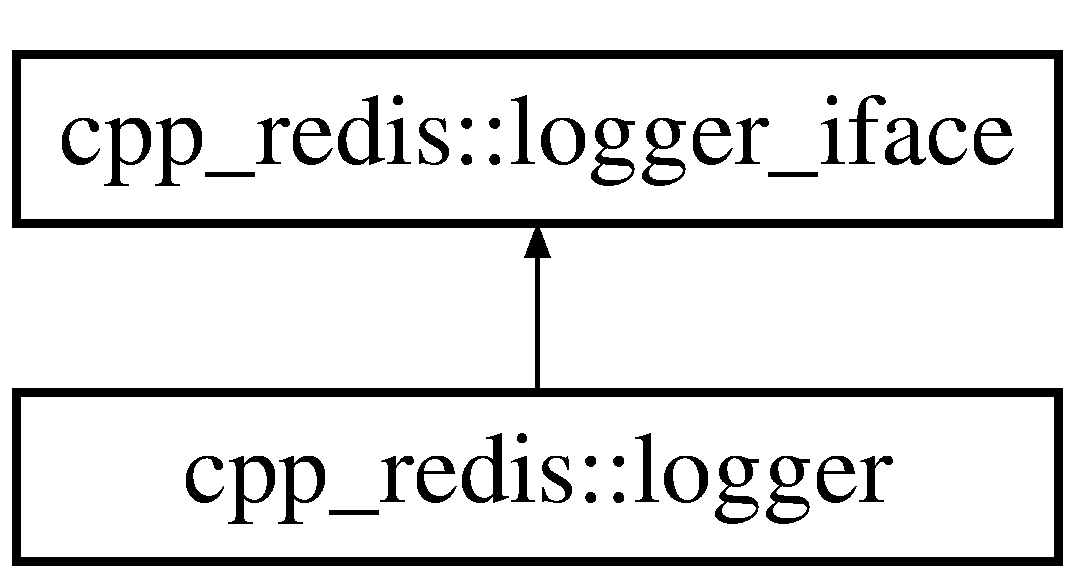
\includegraphics[height=2.000000cm]{classcpp__redis_1_1logger__iface}
\end{center}
\end{figure}
\subsection*{Public Member Functions}
\begin{DoxyCompactItemize}
\item 
\mbox{\Hypertarget{classcpp__redis_1_1logger__iface_a902e41bf0777b960b6575e7ac986147b}\label{classcpp__redis_1_1logger__iface_a902e41bf0777b960b6575e7ac986147b}} 
\hyperlink{classcpp__redis_1_1logger__iface_a902e41bf0777b960b6575e7ac986147b}{logger\+\_\+iface} (void)=default
\begin{DoxyCompactList}\small\item\em ctor \end{DoxyCompactList}\item 
\mbox{\Hypertarget{classcpp__redis_1_1logger__iface_ac7ed1b828afd2e6589fcdda167d34aa5}\label{classcpp__redis_1_1logger__iface_ac7ed1b828afd2e6589fcdda167d34aa5}} 
virtual \hyperlink{classcpp__redis_1_1logger__iface_ac7ed1b828afd2e6589fcdda167d34aa5}{$\sim$logger\+\_\+iface} (void)=default
\begin{DoxyCompactList}\small\item\em dtor \end{DoxyCompactList}\item 
\mbox{\Hypertarget{classcpp__redis_1_1logger__iface_a7f1cb271b18e40f2dde7e45028e69a84}\label{classcpp__redis_1_1logger__iface_a7f1cb271b18e40f2dde7e45028e69a84}} 
\hyperlink{classcpp__redis_1_1logger__iface_a7f1cb271b18e40f2dde7e45028e69a84}{logger\+\_\+iface} (const \hyperlink{classcpp__redis_1_1logger__iface}{logger\+\_\+iface} \&)=default
\begin{DoxyCompactList}\small\item\em copy ctor \end{DoxyCompactList}\item 
\mbox{\Hypertarget{classcpp__redis_1_1logger__iface_a04324701cb81ba6a23f73025b0b3eee0}\label{classcpp__redis_1_1logger__iface_a04324701cb81ba6a23f73025b0b3eee0}} 
\hyperlink{classcpp__redis_1_1logger__iface}{logger\+\_\+iface} \& \hyperlink{classcpp__redis_1_1logger__iface_a04324701cb81ba6a23f73025b0b3eee0}{operator=} (const \hyperlink{classcpp__redis_1_1logger__iface}{logger\+\_\+iface} \&)=default
\begin{DoxyCompactList}\small\item\em assignment operator \end{DoxyCompactList}\item 
virtual void \hyperlink{classcpp__redis_1_1logger__iface_aaace9e12cbb32d7bdd76c17180a30de7}{debug} (const std\+::string \&msg, const std\+::string \&file, std\+::size\+\_\+t line)=0
\item 
virtual void \hyperlink{classcpp__redis_1_1logger__iface_a02e62f55d7da56efa3b47f2b05931b3b}{info} (const std\+::string \&msg, const std\+::string \&file, std\+::size\+\_\+t line)=0
\item 
virtual void \hyperlink{classcpp__redis_1_1logger__iface_a0ea8e43a4f2118e77af56cd1cdb21cba}{warn} (const std\+::string \&msg, const std\+::string \&file, std\+::size\+\_\+t line)=0
\item 
virtual void \hyperlink{classcpp__redis_1_1logger__iface_ac8353031252c80e69e35f5f131870ddf}{error} (const std\+::string \&msg, const std\+::string \&file, std\+::size\+\_\+t line)=0
\end{DoxyCompactItemize}


\subsection{Detailed Description}
\hyperlink{classcpp__redis_1_1logger__iface}{logger\+\_\+iface} should be inherited by any class intended to be used for logging 

\subsection{Member Function Documentation}
\mbox{\Hypertarget{classcpp__redis_1_1logger__iface_aaace9e12cbb32d7bdd76c17180a30de7}\label{classcpp__redis_1_1logger__iface_aaace9e12cbb32d7bdd76c17180a30de7}} 
\index{cpp\+\_\+redis\+::logger\+\_\+iface@{cpp\+\_\+redis\+::logger\+\_\+iface}!debug@{debug}}
\index{debug@{debug}!cpp\+\_\+redis\+::logger\+\_\+iface@{cpp\+\_\+redis\+::logger\+\_\+iface}}
\subsubsection{\texorpdfstring{debug()}{debug()}}
{\footnotesize\ttfamily virtual void cpp\+\_\+redis\+::logger\+\_\+iface\+::debug (\begin{DoxyParamCaption}\item[{const std\+::string \&}]{msg,  }\item[{const std\+::string \&}]{file,  }\item[{std\+::size\+\_\+t}]{line }\end{DoxyParamCaption})\hspace{0.3cm}{\ttfamily [pure virtual]}}

debug logging


\begin{DoxyParams}{Parameters}
{\em msg} & message to be logged \\
\hline
{\em file} & file from which the message is coming \\
\hline
{\em line} & line in the file of the message \\
\hline
\end{DoxyParams}


Implemented in \hyperlink{classcpp__redis_1_1logger_a36e0908e7b05850b663a4b8b9cdbc299}{cpp\+\_\+redis\+::logger}.

\mbox{\Hypertarget{classcpp__redis_1_1logger__iface_ac8353031252c80e69e35f5f131870ddf}\label{classcpp__redis_1_1logger__iface_ac8353031252c80e69e35f5f131870ddf}} 
\index{cpp\+\_\+redis\+::logger\+\_\+iface@{cpp\+\_\+redis\+::logger\+\_\+iface}!error@{error}}
\index{error@{error}!cpp\+\_\+redis\+::logger\+\_\+iface@{cpp\+\_\+redis\+::logger\+\_\+iface}}
\subsubsection{\texorpdfstring{error()}{error()}}
{\footnotesize\ttfamily virtual void cpp\+\_\+redis\+::logger\+\_\+iface\+::error (\begin{DoxyParamCaption}\item[{const std\+::string \&}]{msg,  }\item[{const std\+::string \&}]{file,  }\item[{std\+::size\+\_\+t}]{line }\end{DoxyParamCaption})\hspace{0.3cm}{\ttfamily [pure virtual]}}

error logging


\begin{DoxyParams}{Parameters}
{\em msg} & message to be logged \\
\hline
{\em file} & file from which the message is coming \\
\hline
{\em line} & line in the file of the message \\
\hline
\end{DoxyParams}


Implemented in \hyperlink{classcpp__redis_1_1logger_aaf7f2837511f4414a4d7b7b923ebc15e}{cpp\+\_\+redis\+::logger}.

\mbox{\Hypertarget{classcpp__redis_1_1logger__iface_a02e62f55d7da56efa3b47f2b05931b3b}\label{classcpp__redis_1_1logger__iface_a02e62f55d7da56efa3b47f2b05931b3b}} 
\index{cpp\+\_\+redis\+::logger\+\_\+iface@{cpp\+\_\+redis\+::logger\+\_\+iface}!info@{info}}
\index{info@{info}!cpp\+\_\+redis\+::logger\+\_\+iface@{cpp\+\_\+redis\+::logger\+\_\+iface}}
\subsubsection{\texorpdfstring{info()}{info()}}
{\footnotesize\ttfamily virtual void cpp\+\_\+redis\+::logger\+\_\+iface\+::info (\begin{DoxyParamCaption}\item[{const std\+::string \&}]{msg,  }\item[{const std\+::string \&}]{file,  }\item[{std\+::size\+\_\+t}]{line }\end{DoxyParamCaption})\hspace{0.3cm}{\ttfamily [pure virtual]}}

info logging


\begin{DoxyParams}{Parameters}
{\em msg} & message to be logged \\
\hline
{\em file} & file from which the message is coming \\
\hline
{\em line} & line in the file of the message \\
\hline
\end{DoxyParams}


Implemented in \hyperlink{classcpp__redis_1_1logger_a04c741b5110946e76bb23728da6fb2ac}{cpp\+\_\+redis\+::logger}.

\mbox{\Hypertarget{classcpp__redis_1_1logger__iface_a0ea8e43a4f2118e77af56cd1cdb21cba}\label{classcpp__redis_1_1logger__iface_a0ea8e43a4f2118e77af56cd1cdb21cba}} 
\index{cpp\+\_\+redis\+::logger\+\_\+iface@{cpp\+\_\+redis\+::logger\+\_\+iface}!warn@{warn}}
\index{warn@{warn}!cpp\+\_\+redis\+::logger\+\_\+iface@{cpp\+\_\+redis\+::logger\+\_\+iface}}
\subsubsection{\texorpdfstring{warn()}{warn()}}
{\footnotesize\ttfamily virtual void cpp\+\_\+redis\+::logger\+\_\+iface\+::warn (\begin{DoxyParamCaption}\item[{const std\+::string \&}]{msg,  }\item[{const std\+::string \&}]{file,  }\item[{std\+::size\+\_\+t}]{line }\end{DoxyParamCaption})\hspace{0.3cm}{\ttfamily [pure virtual]}}

warn logging


\begin{DoxyParams}{Parameters}
{\em msg} & message to be logged \\
\hline
{\em file} & file from which the message is coming \\
\hline
{\em line} & line in the file of the message \\
\hline
\end{DoxyParams}


Implemented in \hyperlink{classcpp__redis_1_1logger_ae9359429428786c7b5605a1109508ae5}{cpp\+\_\+redis\+::logger}.



The documentation for this class was generated from the following file\+:\begin{DoxyCompactItemize}
\item 
includes/cpp\+\_\+redis/misc/logger.\+hpp\end{DoxyCompactItemize}

\hypertarget{structcpp__redis_1_1network_1_1tcp__client__iface_1_1read__request}{}\section{cpp\+\_\+redis\+:\+:network\+:\+:tcp\+\_\+client\+\_\+iface\+:\+:read\+\_\+request Struct Reference}
\label{structcpp__redis_1_1network_1_1tcp__client__iface_1_1read__request}\index{cpp\+\_\+redis\+::network\+::tcp\+\_\+client\+\_\+iface\+::read\+\_\+request@{cpp\+\_\+redis\+::network\+::tcp\+\_\+client\+\_\+iface\+::read\+\_\+request}}


{\ttfamily \#include $<$tcp\+\_\+client\+\_\+iface.\+hpp$>$}

\subsection*{Public Attributes}
\begin{DoxyCompactItemize}
\item 
std\+::size\+\_\+t \hyperlink{structcpp__redis_1_1network_1_1tcp__client__iface_1_1read__request_a5ff8258391c9b3c8d2ce1a5c5a0304be}{size}
\item 
\hyperlink{classcpp__redis_1_1network_1_1tcp__client__iface_ae8bf79e8e1f1d7e359ed1c7cdc4026fc}{async\+\_\+read\+\_\+callback\+\_\+t} \hyperlink{structcpp__redis_1_1network_1_1tcp__client__iface_1_1read__request_a0584269b3a021d588e38948c12fa5292}{async\+\_\+read\+\_\+callback}
\end{DoxyCompactItemize}


\subsection{Detailed Description}
structure to store read requests information 

\subsection{Member Data Documentation}
\mbox{\Hypertarget{structcpp__redis_1_1network_1_1tcp__client__iface_1_1read__request_a0584269b3a021d588e38948c12fa5292}\label{structcpp__redis_1_1network_1_1tcp__client__iface_1_1read__request_a0584269b3a021d588e38948c12fa5292}} 
\index{cpp\+\_\+redis\+::network\+::tcp\+\_\+client\+\_\+iface\+::read\+\_\+request@{cpp\+\_\+redis\+::network\+::tcp\+\_\+client\+\_\+iface\+::read\+\_\+request}!async\+\_\+read\+\_\+callback@{async\+\_\+read\+\_\+callback}}
\index{async\+\_\+read\+\_\+callback@{async\+\_\+read\+\_\+callback}!cpp\+\_\+redis\+::network\+::tcp\+\_\+client\+\_\+iface\+::read\+\_\+request@{cpp\+\_\+redis\+::network\+::tcp\+\_\+client\+\_\+iface\+::read\+\_\+request}}
\subsubsection{\texorpdfstring{async\+\_\+read\+\_\+callback}{async\_read\_callback}}
{\footnotesize\ttfamily \hyperlink{classcpp__redis_1_1network_1_1tcp__client__iface_ae8bf79e8e1f1d7e359ed1c7cdc4026fc}{async\+\_\+read\+\_\+callback\+\_\+t} cpp\+\_\+redis\+::network\+::tcp\+\_\+client\+\_\+iface\+::read\+\_\+request\+::async\+\_\+read\+\_\+callback}

callback to be called on operation completion \mbox{\Hypertarget{structcpp__redis_1_1network_1_1tcp__client__iface_1_1read__request_a5ff8258391c9b3c8d2ce1a5c5a0304be}\label{structcpp__redis_1_1network_1_1tcp__client__iface_1_1read__request_a5ff8258391c9b3c8d2ce1a5c5a0304be}} 
\index{cpp\+\_\+redis\+::network\+::tcp\+\_\+client\+\_\+iface\+::read\+\_\+request@{cpp\+\_\+redis\+::network\+::tcp\+\_\+client\+\_\+iface\+::read\+\_\+request}!size@{size}}
\index{size@{size}!cpp\+\_\+redis\+::network\+::tcp\+\_\+client\+\_\+iface\+::read\+\_\+request@{cpp\+\_\+redis\+::network\+::tcp\+\_\+client\+\_\+iface\+::read\+\_\+request}}
\subsubsection{\texorpdfstring{size}{size}}
{\footnotesize\ttfamily std\+::size\+\_\+t cpp\+\_\+redis\+::network\+::tcp\+\_\+client\+\_\+iface\+::read\+\_\+request\+::size}

number of bytes to read 

The documentation for this struct was generated from the following file\+:\begin{DoxyCompactItemize}
\item 
includes/cpp\+\_\+redis/network/tcp\+\_\+client\+\_\+iface.\+hpp\end{DoxyCompactItemize}

\hypertarget{structcpp__redis_1_1network_1_1tcp__client__iface_1_1read__result}{}\section{cpp\+\_\+redis\+:\+:network\+:\+:tcp\+\_\+client\+\_\+iface\+:\+:read\+\_\+result Struct Reference}
\label{structcpp__redis_1_1network_1_1tcp__client__iface_1_1read__result}\index{cpp\+\_\+redis\+::network\+::tcp\+\_\+client\+\_\+iface\+::read\+\_\+result@{cpp\+\_\+redis\+::network\+::tcp\+\_\+client\+\_\+iface\+::read\+\_\+result}}


{\ttfamily \#include $<$tcp\+\_\+client\+\_\+iface.\+hpp$>$}

\subsection*{Public Attributes}
\begin{DoxyCompactItemize}
\item 
bool \hyperlink{structcpp__redis_1_1network_1_1tcp__client__iface_1_1read__result_ab9a3a54474c382a00323ed02f4239faa}{success}
\item 
std\+::vector$<$ char $>$ \hyperlink{structcpp__redis_1_1network_1_1tcp__client__iface_1_1read__result_af8275097ebe558e7ce0f2aa29131cb05}{buffer}
\end{DoxyCompactItemize}


\subsection{Detailed Description}
structure to store read requests result 

\subsection{Member Data Documentation}
\mbox{\Hypertarget{structcpp__redis_1_1network_1_1tcp__client__iface_1_1read__result_af8275097ebe558e7ce0f2aa29131cb05}\label{structcpp__redis_1_1network_1_1tcp__client__iface_1_1read__result_af8275097ebe558e7ce0f2aa29131cb05}} 
\index{cpp\+\_\+redis\+::network\+::tcp\+\_\+client\+\_\+iface\+::read\+\_\+result@{cpp\+\_\+redis\+::network\+::tcp\+\_\+client\+\_\+iface\+::read\+\_\+result}!buffer@{buffer}}
\index{buffer@{buffer}!cpp\+\_\+redis\+::network\+::tcp\+\_\+client\+\_\+iface\+::read\+\_\+result@{cpp\+\_\+redis\+::network\+::tcp\+\_\+client\+\_\+iface\+::read\+\_\+result}}
\subsubsection{\texorpdfstring{buffer}{buffer}}
{\footnotesize\ttfamily std\+::vector$<$char$>$ cpp\+\_\+redis\+::network\+::tcp\+\_\+client\+\_\+iface\+::read\+\_\+result\+::buffer}

read bytes \mbox{\Hypertarget{structcpp__redis_1_1network_1_1tcp__client__iface_1_1read__result_ab9a3a54474c382a00323ed02f4239faa}\label{structcpp__redis_1_1network_1_1tcp__client__iface_1_1read__result_ab9a3a54474c382a00323ed02f4239faa}} 
\index{cpp\+\_\+redis\+::network\+::tcp\+\_\+client\+\_\+iface\+::read\+\_\+result@{cpp\+\_\+redis\+::network\+::tcp\+\_\+client\+\_\+iface\+::read\+\_\+result}!success@{success}}
\index{success@{success}!cpp\+\_\+redis\+::network\+::tcp\+\_\+client\+\_\+iface\+::read\+\_\+result@{cpp\+\_\+redis\+::network\+::tcp\+\_\+client\+\_\+iface\+::read\+\_\+result}}
\subsubsection{\texorpdfstring{success}{success}}
{\footnotesize\ttfamily bool cpp\+\_\+redis\+::network\+::tcp\+\_\+client\+\_\+iface\+::read\+\_\+result\+::success}

whether the operation succeeded or not 

The documentation for this struct was generated from the following file\+:\begin{DoxyCompactItemize}
\item 
includes/cpp\+\_\+redis/network/tcp\+\_\+client\+\_\+iface.\+hpp\end{DoxyCompactItemize}

\hypertarget{classcpp__redis_1_1network_1_1redis__connection}{}\section{cpp\+\_\+redis\+:\+:network\+:\+:redis\+\_\+connection Class Reference}
\label{classcpp__redis_1_1network_1_1redis__connection}\index{cpp\+\_\+redis\+::network\+::redis\+\_\+connection@{cpp\+\_\+redis\+::network\+::redis\+\_\+connection}}


{\ttfamily \#include $<$redis\+\_\+connection.\+hpp$>$}

\subsection*{Public Types}
\begin{DoxyCompactItemize}
\item 
typedef std\+::function$<$ void(\hyperlink{classcpp__redis_1_1network_1_1redis__connection}{redis\+\_\+connection} \&)$>$ \hyperlink{classcpp__redis_1_1network_1_1redis__connection_aba1a229a3d36a5540a80776ed0cf9a44}{disconnection\+\_\+handler\+\_\+t}
\item 
typedef std\+::function$<$ void(\hyperlink{classcpp__redis_1_1network_1_1redis__connection}{redis\+\_\+connection} \&, \hyperlink{classcpp__redis_1_1reply}{reply} \&)$>$ \hyperlink{classcpp__redis_1_1network_1_1redis__connection_a40f4b55a3103b7436e34211893377245}{reply\+\_\+callback\+\_\+t}
\end{DoxyCompactItemize}
\subsection*{Public Member Functions}
\begin{DoxyCompactItemize}
\item 
\mbox{\Hypertarget{classcpp__redis_1_1network_1_1redis__connection_aee0302e4ff9c9b5b2e7f467d869d45f7}\label{classcpp__redis_1_1network_1_1redis__connection_aee0302e4ff9c9b5b2e7f467d869d45f7}} 
\hyperlink{classcpp__redis_1_1network_1_1redis__connection_aee0302e4ff9c9b5b2e7f467d869d45f7}{redis\+\_\+connection} (void)
\begin{DoxyCompactList}\small\item\em ctor \end{DoxyCompactList}\item 
\hyperlink{classcpp__redis_1_1network_1_1redis__connection_a6880cfb2e1b037fcdaa5f0a6d515b375}{redis\+\_\+connection} (const std\+::shared\+\_\+ptr$<$ \hyperlink{classcpp__redis_1_1network_1_1tcp__client__iface}{tcp\+\_\+client\+\_\+iface} $>$ \&\hyperlink{classcpp__redis_1_1network_1_1tcp__client}{tcp\+\_\+client})
\item 
\mbox{\Hypertarget{classcpp__redis_1_1network_1_1redis__connection_a9d392191ce262eddd5570b57e07aa051}\label{classcpp__redis_1_1network_1_1redis__connection_a9d392191ce262eddd5570b57e07aa051}} 
\hyperlink{classcpp__redis_1_1network_1_1redis__connection_a9d392191ce262eddd5570b57e07aa051}{$\sim$redis\+\_\+connection} (void)
\begin{DoxyCompactList}\small\item\em dtor \end{DoxyCompactList}\item 
\mbox{\Hypertarget{classcpp__redis_1_1network_1_1redis__connection_a2bdd38bbfd5d97aeca8e433465c4d621}\label{classcpp__redis_1_1network_1_1redis__connection_a2bdd38bbfd5d97aeca8e433465c4d621}} 
\hyperlink{classcpp__redis_1_1network_1_1redis__connection_a2bdd38bbfd5d97aeca8e433465c4d621}{redis\+\_\+connection} (const \hyperlink{classcpp__redis_1_1network_1_1redis__connection}{redis\+\_\+connection} \&)=delete
\begin{DoxyCompactList}\small\item\em copy ctor \end{DoxyCompactList}\item 
\mbox{\Hypertarget{classcpp__redis_1_1network_1_1redis__connection_a54a4c28ad1b9e9f3bac2854fddf4e30d}\label{classcpp__redis_1_1network_1_1redis__connection_a54a4c28ad1b9e9f3bac2854fddf4e30d}} 
\hyperlink{classcpp__redis_1_1network_1_1redis__connection}{redis\+\_\+connection} \& \hyperlink{classcpp__redis_1_1network_1_1redis__connection_a54a4c28ad1b9e9f3bac2854fddf4e30d}{operator=} (const \hyperlink{classcpp__redis_1_1network_1_1redis__connection}{redis\+\_\+connection} \&)=delete
\begin{DoxyCompactList}\small\item\em assignment operator \end{DoxyCompactList}\item 
void \hyperlink{classcpp__redis_1_1network_1_1redis__connection_af105573e46eadbc34a9f5907832df19f}{connect} (const std\+::string \&host=\char`\"{}127.\+0.\+0.\+1\char`\"{}, std\+::size\+\_\+t port=6379, const \hyperlink{classcpp__redis_1_1network_1_1redis__connection_aba1a229a3d36a5540a80776ed0cf9a44}{disconnection\+\_\+handler\+\_\+t} \&disconnection\+\_\+handler=nullptr, const \hyperlink{classcpp__redis_1_1network_1_1redis__connection_a40f4b55a3103b7436e34211893377245}{reply\+\_\+callback\+\_\+t} \&reply\+\_\+callback=nullptr, std\+::uint32\+\_\+t timeout\+\_\+msecs=0)
\item 
void \hyperlink{classcpp__redis_1_1network_1_1redis__connection_abdeb36976c0a0e5cc16d7ba4259e7e49}{disconnect} (void)
\item 
bool \hyperlink{classcpp__redis_1_1network_1_1redis__connection_ad3d96826e2e67fb3fed23280237d4d9c}{is\+\_\+connected} (void) const
\item 
\hyperlink{classcpp__redis_1_1network_1_1redis__connection}{redis\+\_\+connection} \& \hyperlink{classcpp__redis_1_1network_1_1redis__connection_a98c163ce431e85e46e139211564b7b3f}{send} (const std\+::vector$<$ std\+::string $>$ \&redis\+\_\+cmd)
\item 
\hyperlink{classcpp__redis_1_1network_1_1redis__connection}{redis\+\_\+connection} \& \hyperlink{classcpp__redis_1_1network_1_1redis__connection_a8e6980d40139877c16e995051b780d60}{commit} (void)
\end{DoxyCompactItemize}


\subsection{Detailed Description}
tcp connection wrapper handling redis protocol 

\subsection{Member Typedef Documentation}
\mbox{\Hypertarget{classcpp__redis_1_1network_1_1redis__connection_aba1a229a3d36a5540a80776ed0cf9a44}\label{classcpp__redis_1_1network_1_1redis__connection_aba1a229a3d36a5540a80776ed0cf9a44}} 
\index{cpp\+\_\+redis\+::network\+::redis\+\_\+connection@{cpp\+\_\+redis\+::network\+::redis\+\_\+connection}!disconnection\+\_\+handler\+\_\+t@{disconnection\+\_\+handler\+\_\+t}}
\index{disconnection\+\_\+handler\+\_\+t@{disconnection\+\_\+handler\+\_\+t}!cpp\+\_\+redis\+::network\+::redis\+\_\+connection@{cpp\+\_\+redis\+::network\+::redis\+\_\+connection}}
\subsubsection{\texorpdfstring{disconnection\+\_\+handler\+\_\+t}{disconnection\_handler\_t}}
{\footnotesize\ttfamily typedef std\+::function$<$void(\hyperlink{classcpp__redis_1_1network_1_1redis__connection}{redis\+\_\+connection}\&)$>$ \hyperlink{classcpp__redis_1_1network_1_1redis__connection_aba1a229a3d36a5540a80776ed0cf9a44}{cpp\+\_\+redis\+::network\+::redis\+\_\+connection\+::disconnection\+\_\+handler\+\_\+t}}

disconnection handler takes as parameter the instance of the \hyperlink{classcpp__redis_1_1network_1_1redis__connection}{redis\+\_\+connection} \mbox{\Hypertarget{classcpp__redis_1_1network_1_1redis__connection_a40f4b55a3103b7436e34211893377245}\label{classcpp__redis_1_1network_1_1redis__connection_a40f4b55a3103b7436e34211893377245}} 
\index{cpp\+\_\+redis\+::network\+::redis\+\_\+connection@{cpp\+\_\+redis\+::network\+::redis\+\_\+connection}!reply\+\_\+callback\+\_\+t@{reply\+\_\+callback\+\_\+t}}
\index{reply\+\_\+callback\+\_\+t@{reply\+\_\+callback\+\_\+t}!cpp\+\_\+redis\+::network\+::redis\+\_\+connection@{cpp\+\_\+redis\+::network\+::redis\+\_\+connection}}
\subsubsection{\texorpdfstring{reply\+\_\+callback\+\_\+t}{reply\_callback\_t}}
{\footnotesize\ttfamily typedef std\+::function$<$void(\hyperlink{classcpp__redis_1_1network_1_1redis__connection}{redis\+\_\+connection}\&, \hyperlink{classcpp__redis_1_1reply}{reply}\&)$>$ \hyperlink{classcpp__redis_1_1network_1_1redis__connection_a40f4b55a3103b7436e34211893377245}{cpp\+\_\+redis\+::network\+::redis\+\_\+connection\+::reply\+\_\+callback\+\_\+t}}

reply handler takes as parameter the instance of the \hyperlink{classcpp__redis_1_1network_1_1redis__connection}{redis\+\_\+connection} and the built reply 

\subsection{Constructor \& Destructor Documentation}
\mbox{\Hypertarget{classcpp__redis_1_1network_1_1redis__connection_a6880cfb2e1b037fcdaa5f0a6d515b375}\label{classcpp__redis_1_1network_1_1redis__connection_a6880cfb2e1b037fcdaa5f0a6d515b375}} 
\index{cpp\+\_\+redis\+::network\+::redis\+\_\+connection@{cpp\+\_\+redis\+::network\+::redis\+\_\+connection}!redis\+\_\+connection@{redis\+\_\+connection}}
\index{redis\+\_\+connection@{redis\+\_\+connection}!cpp\+\_\+redis\+::network\+::redis\+\_\+connection@{cpp\+\_\+redis\+::network\+::redis\+\_\+connection}}
\subsubsection{\texorpdfstring{redis\+\_\+connection()}{redis\_connection()}}
{\footnotesize\ttfamily cpp\+\_\+redis\+::network\+::redis\+\_\+connection\+::redis\+\_\+connection (\begin{DoxyParamCaption}\item[{const std\+::shared\+\_\+ptr$<$ \hyperlink{classcpp__redis_1_1network_1_1tcp__client__iface}{tcp\+\_\+client\+\_\+iface} $>$ \&}]{tcp\+\_\+client }\end{DoxyParamCaption})\hspace{0.3cm}{\ttfamily [explicit]}}

ctor allowing to specify custom tcp client (default ctor uses the default tacopie tcp client)


\begin{DoxyParams}{Parameters}
{\em \hyperlink{classcpp__redis_1_1network_1_1tcp__client}{tcp\+\_\+client}} & tcp client to be used for network communications \\
\hline
\end{DoxyParams}


\subsection{Member Function Documentation}
\mbox{\Hypertarget{classcpp__redis_1_1network_1_1redis__connection_a8e6980d40139877c16e995051b780d60}\label{classcpp__redis_1_1network_1_1redis__connection_a8e6980d40139877c16e995051b780d60}} 
\index{cpp\+\_\+redis\+::network\+::redis\+\_\+connection@{cpp\+\_\+redis\+::network\+::redis\+\_\+connection}!commit@{commit}}
\index{commit@{commit}!cpp\+\_\+redis\+::network\+::redis\+\_\+connection@{cpp\+\_\+redis\+::network\+::redis\+\_\+connection}}
\subsubsection{\texorpdfstring{commit()}{commit()}}
{\footnotesize\ttfamily \hyperlink{classcpp__redis_1_1network_1_1redis__connection}{redis\+\_\+connection}\& cpp\+\_\+redis\+::network\+::redis\+\_\+connection\+::commit (\begin{DoxyParamCaption}\item[{void}]{ }\end{DoxyParamCaption})}

commit pipelined transaction that is, send to the network all commands pipelined by calling \hyperlink{classcpp__redis_1_1network_1_1redis__connection_a98c163ce431e85e46e139211564b7b3f}{send()}

\begin{DoxyReturn}{Returns}
current instance 
\end{DoxyReturn}
\mbox{\Hypertarget{classcpp__redis_1_1network_1_1redis__connection_af105573e46eadbc34a9f5907832df19f}\label{classcpp__redis_1_1network_1_1redis__connection_af105573e46eadbc34a9f5907832df19f}} 
\index{cpp\+\_\+redis\+::network\+::redis\+\_\+connection@{cpp\+\_\+redis\+::network\+::redis\+\_\+connection}!connect@{connect}}
\index{connect@{connect}!cpp\+\_\+redis\+::network\+::redis\+\_\+connection@{cpp\+\_\+redis\+::network\+::redis\+\_\+connection}}
\subsubsection{\texorpdfstring{connect()}{connect()}}
{\footnotesize\ttfamily void cpp\+\_\+redis\+::network\+::redis\+\_\+connection\+::connect (\begin{DoxyParamCaption}\item[{const std\+::string \&}]{host = {\ttfamily \char`\"{}127.0.0.1\char`\"{}},  }\item[{std\+::size\+\_\+t}]{port = {\ttfamily 6379},  }\item[{const \hyperlink{classcpp__redis_1_1network_1_1redis__connection_aba1a229a3d36a5540a80776ed0cf9a44}{disconnection\+\_\+handler\+\_\+t} \&}]{disconnection\+\_\+handler = {\ttfamily nullptr},  }\item[{const \hyperlink{classcpp__redis_1_1network_1_1redis__connection_a40f4b55a3103b7436e34211893377245}{reply\+\_\+callback\+\_\+t} \&}]{reply\+\_\+callback = {\ttfamily nullptr},  }\item[{std\+::uint32\+\_\+t}]{timeout\+\_\+msecs = {\ttfamily 0} }\end{DoxyParamCaption})}

connect to the given host and port, and set both disconnection and reply callbacks


\begin{DoxyParams}{Parameters}
{\em host} & host to be connected to \\
\hline
{\em port} & port to be connected to \\
\hline
{\em disconnection\+\_\+handler} & handler to be called in case of disconnection \\
\hline
{\em reply\+\_\+callback} & handler to be called once a reply is ready \\
\hline
{\em timeout\+\_\+msecs} & max time to connect (in ms) \\
\hline
\end{DoxyParams}
\mbox{\Hypertarget{classcpp__redis_1_1network_1_1redis__connection_abdeb36976c0a0e5cc16d7ba4259e7e49}\label{classcpp__redis_1_1network_1_1redis__connection_abdeb36976c0a0e5cc16d7ba4259e7e49}} 
\index{cpp\+\_\+redis\+::network\+::redis\+\_\+connection@{cpp\+\_\+redis\+::network\+::redis\+\_\+connection}!disconnect@{disconnect}}
\index{disconnect@{disconnect}!cpp\+\_\+redis\+::network\+::redis\+\_\+connection@{cpp\+\_\+redis\+::network\+::redis\+\_\+connection}}
\subsubsection{\texorpdfstring{disconnect()}{disconnect()}}
{\footnotesize\ttfamily void cpp\+\_\+redis\+::network\+::redis\+\_\+connection\+::disconnect (\begin{DoxyParamCaption}\item[{void}]{ }\end{DoxyParamCaption})}

disconnect from redis server \mbox{\Hypertarget{classcpp__redis_1_1network_1_1redis__connection_ad3d96826e2e67fb3fed23280237d4d9c}\label{classcpp__redis_1_1network_1_1redis__connection_ad3d96826e2e67fb3fed23280237d4d9c}} 
\index{cpp\+\_\+redis\+::network\+::redis\+\_\+connection@{cpp\+\_\+redis\+::network\+::redis\+\_\+connection}!is\+\_\+connected@{is\+\_\+connected}}
\index{is\+\_\+connected@{is\+\_\+connected}!cpp\+\_\+redis\+::network\+::redis\+\_\+connection@{cpp\+\_\+redis\+::network\+::redis\+\_\+connection}}
\subsubsection{\texorpdfstring{is\+\_\+connected()}{is\_connected()}}
{\footnotesize\ttfamily bool cpp\+\_\+redis\+::network\+::redis\+\_\+connection\+::is\+\_\+connected (\begin{DoxyParamCaption}\item[{void}]{ }\end{DoxyParamCaption}) const}

\begin{DoxyReturn}{Returns}
whether we are connected to the redis server or not 
\end{DoxyReturn}
\mbox{\Hypertarget{classcpp__redis_1_1network_1_1redis__connection_a98c163ce431e85e46e139211564b7b3f}\label{classcpp__redis_1_1network_1_1redis__connection_a98c163ce431e85e46e139211564b7b3f}} 
\index{cpp\+\_\+redis\+::network\+::redis\+\_\+connection@{cpp\+\_\+redis\+::network\+::redis\+\_\+connection}!send@{send}}
\index{send@{send}!cpp\+\_\+redis\+::network\+::redis\+\_\+connection@{cpp\+\_\+redis\+::network\+::redis\+\_\+connection}}
\subsubsection{\texorpdfstring{send()}{send()}}
{\footnotesize\ttfamily \hyperlink{classcpp__redis_1_1network_1_1redis__connection}{redis\+\_\+connection}\& cpp\+\_\+redis\+::network\+::redis\+\_\+connection\+::send (\begin{DoxyParamCaption}\item[{const std\+::vector$<$ std\+::string $>$ \&}]{redis\+\_\+cmd }\end{DoxyParamCaption})}

send the given command the command is actually pipelined and only buffered, so nothing is sent to the network please call \hyperlink{classcpp__redis_1_1network_1_1redis__connection_a8e6980d40139877c16e995051b780d60}{commit()} to flush the buffer


\begin{DoxyParams}{Parameters}
{\em redis\+\_\+cmd} & command to be sent \\
\hline
\end{DoxyParams}
\begin{DoxyReturn}{Returns}
current instance 
\end{DoxyReturn}


The documentation for this class was generated from the following file\+:\begin{DoxyCompactItemize}
\item 
includes/cpp\+\_\+redis/network/redis\+\_\+connection.\+hpp\end{DoxyCompactItemize}

\hypertarget{classcpp__redis_1_1redis__error}{}\section{cpp\+\_\+redis\+:\+:redis\+\_\+error Class Reference}
\label{classcpp__redis_1_1redis__error}\index{cpp\+\_\+redis\+::redis\+\_\+error@{cpp\+\_\+redis\+::redis\+\_\+error}}


{\ttfamily \#include $<$error.\+hpp$>$}

Inheritance diagram for cpp\+\_\+redis\+:\+:redis\+\_\+error\+:\begin{figure}[H]
\begin{center}
\leavevmode
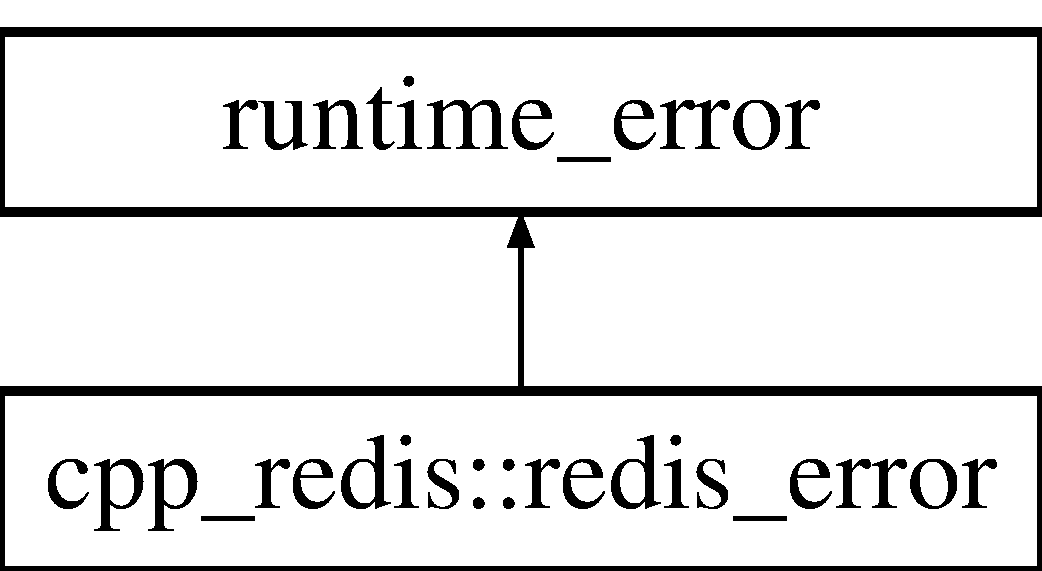
\includegraphics[height=2.000000cm]{classcpp__redis_1_1redis__error}
\end{center}
\end{figure}
\subsection*{Public Member Functions}
\begin{DoxyCompactItemize}
\item 
\hyperlink{classcpp__redis_1_1redis__error_a1445e654b3936c7f5aa1c298bcf24966}{redis\+\_\+error} (const std\+::string \&err)
\begin{DoxyCompactList}\small\item\em ctor (string) \end{DoxyCompactList}\item 
\hyperlink{classcpp__redis_1_1redis__error_a0ced25483119c2318b1a5a69cac1919f}{redis\+\_\+error} (const char $\ast$err)
\begin{DoxyCompactList}\small\item\em ctor(char$\ast$) \end{DoxyCompactList}\end{DoxyCompactItemize}


\subsection{Detailed Description}
specialized runtime\+\_\+error used for \hyperlink{namespacecpp__redis}{cpp\+\_\+redis} error 

\subsection{Constructor \& Destructor Documentation}
\mbox{\Hypertarget{classcpp__redis_1_1redis__error_a1445e654b3936c7f5aa1c298bcf24966}\label{classcpp__redis_1_1redis__error_a1445e654b3936c7f5aa1c298bcf24966}} 
\index{cpp\+\_\+redis\+::redis\+\_\+error@{cpp\+\_\+redis\+::redis\+\_\+error}!redis\+\_\+error@{redis\+\_\+error}}
\index{redis\+\_\+error@{redis\+\_\+error}!cpp\+\_\+redis\+::redis\+\_\+error@{cpp\+\_\+redis\+::redis\+\_\+error}}
\subsubsection{\texorpdfstring{redis\+\_\+error()}{redis\_error()}\hspace{0.1cm}{\footnotesize\ttfamily [1/2]}}
{\footnotesize\ttfamily cpp\+\_\+redis\+::redis\+\_\+error\+::redis\+\_\+error (\begin{DoxyParamCaption}\item[{const std\+::string \&}]{err }\end{DoxyParamCaption})\hspace{0.3cm}{\ttfamily [inline]}, {\ttfamily [explicit]}}



ctor (string) 

\mbox{\Hypertarget{classcpp__redis_1_1redis__error_a0ced25483119c2318b1a5a69cac1919f}\label{classcpp__redis_1_1redis__error_a0ced25483119c2318b1a5a69cac1919f}} 
\index{cpp\+\_\+redis\+::redis\+\_\+error@{cpp\+\_\+redis\+::redis\+\_\+error}!redis\+\_\+error@{redis\+\_\+error}}
\index{redis\+\_\+error@{redis\+\_\+error}!cpp\+\_\+redis\+::redis\+\_\+error@{cpp\+\_\+redis\+::redis\+\_\+error}}
\subsubsection{\texorpdfstring{redis\+\_\+error()}{redis\_error()}\hspace{0.1cm}{\footnotesize\ttfamily [2/2]}}
{\footnotesize\ttfamily cpp\+\_\+redis\+::redis\+\_\+error\+::redis\+\_\+error (\begin{DoxyParamCaption}\item[{const char $\ast$}]{err }\end{DoxyParamCaption})\hspace{0.3cm}{\ttfamily [inline]}, {\ttfamily [explicit]}}



ctor(char$\ast$) 



The documentation for this class was generated from the following file\+:\begin{DoxyCompactItemize}
\item 
includes/cpp\+\_\+redis/misc/\hyperlink{error_8hpp}{error.\+hpp}\end{DoxyCompactItemize}

\hypertarget{classcpp__redis_1_1reply}{}\section{cpp\+\_\+redis\+:\+:reply Class Reference}
\label{classcpp__redis_1_1reply}\index{cpp\+\_\+redis\+::reply@{cpp\+\_\+redis\+::reply}}


{\ttfamily \#include $<$reply.\+hpp$>$}

\subsection*{Public Types}
\begin{DoxyCompactItemize}
\item 
enum \hyperlink{classcpp__redis_1_1reply_acc272b2a52164cac1d110c619a0b25bd}{type} \{ \newline
\hyperlink{classcpp__redis_1_1reply_acc272b2a52164cac1d110c619a0b25bdacb5e100e5a9a3e7f6d1fd97512215282}{type\+::error} = \+\_\+\+\_\+\+C\+P\+P\+\_\+\+R\+E\+D\+I\+S\+\_\+\+R\+E\+P\+L\+Y\+\_\+\+E\+RR, 
\hyperlink{classcpp__redis_1_1reply_acc272b2a52164cac1d110c619a0b25bdaffdc5e3d4a1ba77345a59a89c9f70764}{type\+::bulk\+\_\+string} = \+\_\+\+\_\+\+C\+P\+P\+\_\+\+R\+E\+D\+I\+S\+\_\+\+R\+E\+P\+L\+Y\+\_\+\+B\+U\+LK, 
\hyperlink{classcpp__redis_1_1reply_acc272b2a52164cac1d110c619a0b25bda42e59301bab38b6e2a173baf105990dd}{type\+::simple\+\_\+string} = \+\_\+\+\_\+\+C\+P\+P\+\_\+\+R\+E\+D\+I\+S\+\_\+\+R\+E\+P\+L\+Y\+\_\+\+S\+I\+M\+P\+LE, 
\hyperlink{classcpp__redis_1_1reply_acc272b2a52164cac1d110c619a0b25bda37a6259cc0c1dae299a7866489dff0bd}{type\+::null} = \+\_\+\+\_\+\+C\+P\+P\+\_\+\+R\+E\+D\+I\+S\+\_\+\+R\+E\+P\+L\+Y\+\_\+\+N\+U\+LL, 
\newline
\hyperlink{classcpp__redis_1_1reply_acc272b2a52164cac1d110c619a0b25bda157db7df530023575515d366c9b672e8}{type\+::integer} = \+\_\+\+\_\+\+C\+P\+P\+\_\+\+R\+E\+D\+I\+S\+\_\+\+R\+E\+P\+L\+Y\+\_\+\+I\+NT, 
\hyperlink{classcpp__redis_1_1reply_acc272b2a52164cac1d110c619a0b25bdaf1f713c9e000f5d3f280adbd124df4f5}{type\+::array} = \+\_\+\+\_\+\+C\+P\+P\+\_\+\+R\+E\+D\+I\+S\+\_\+\+R\+E\+P\+L\+Y\+\_\+\+A\+R\+R\+AY
 \}
\item 
enum \hyperlink{classcpp__redis_1_1reply_ac192ba4cb8f2bb6e7cb465edf755328b}{string\+\_\+type} \{ \hyperlink{classcpp__redis_1_1reply_ac192ba4cb8f2bb6e7cb465edf755328bacb5e100e5a9a3e7f6d1fd97512215282}{string\+\_\+type\+::error} = \+\_\+\+\_\+\+C\+P\+P\+\_\+\+R\+E\+D\+I\+S\+\_\+\+R\+E\+P\+L\+Y\+\_\+\+E\+RR, 
\hyperlink{classcpp__redis_1_1reply_ac192ba4cb8f2bb6e7cb465edf755328baffdc5e3d4a1ba77345a59a89c9f70764}{string\+\_\+type\+::bulk\+\_\+string} = \+\_\+\+\_\+\+C\+P\+P\+\_\+\+R\+E\+D\+I\+S\+\_\+\+R\+E\+P\+L\+Y\+\_\+\+B\+U\+LK, 
\hyperlink{classcpp__redis_1_1reply_ac192ba4cb8f2bb6e7cb465edf755328ba42e59301bab38b6e2a173baf105990dd}{string\+\_\+type\+::simple\+\_\+string} = \+\_\+\+\_\+\+C\+P\+P\+\_\+\+R\+E\+D\+I\+S\+\_\+\+R\+E\+P\+L\+Y\+\_\+\+S\+I\+M\+P\+LE
 \}
\end{DoxyCompactItemize}
\subsection*{Public Member Functions}
\begin{DoxyCompactItemize}
\item 
\hyperlink{classcpp__redis_1_1reply_a8d0b1f8a18b5c7c3ce79784604dba6cc}{reply} (void)
\item 
\hyperlink{classcpp__redis_1_1reply_a58fb2a051a001f1c3dcf2cd957441dbc}{reply} (const std\+::string \&value, \hyperlink{classcpp__redis_1_1reply_ac192ba4cb8f2bb6e7cb465edf755328b}{string\+\_\+type} reply\+\_\+type)
\item 
\hyperlink{classcpp__redis_1_1reply_a6200b9fa76196e75fb18aa07e47391f0}{reply} (int64\+\_\+t value)
\item 
\hyperlink{classcpp__redis_1_1reply_af3e08b6b795978757a05a1ac4bb08c68}{reply} (const std\+::vector$<$ \hyperlink{classcpp__redis_1_1reply}{reply} $>$ \&rows)
\item 
\hyperlink{classcpp__redis_1_1reply_a1acfe6cbc763368cc2a9eef25afffe35}{$\sim$reply} (void)=default
\begin{DoxyCompactList}\small\item\em dtor \end{DoxyCompactList}\item 
\hyperlink{classcpp__redis_1_1reply_a247955712c519daffcf740ae163e69bb}{reply} (const \hyperlink{classcpp__redis_1_1reply}{reply} \&)=default
\begin{DoxyCompactList}\small\item\em copy ctor \end{DoxyCompactList}\item 
\hyperlink{classcpp__redis_1_1reply}{reply} \& \hyperlink{classcpp__redis_1_1reply_a3482157af73f4a60a6386f057e484e5b}{operator=} (const \hyperlink{classcpp__redis_1_1reply}{reply} \&)=default
\begin{DoxyCompactList}\small\item\em assignment operator \end{DoxyCompactList}\item 
bool \hyperlink{classcpp__redis_1_1reply_a3a94881a46125d281cb36191c4b7d19a}{is\+\_\+array} (void) const
\item 
bool \hyperlink{classcpp__redis_1_1reply_a7072729490fdbad26ddeb02df8002147}{is\+\_\+string} (void) const
\item 
bool \hyperlink{classcpp__redis_1_1reply_aeb92f6f84d226239e9800893ab6062ca}{is\+\_\+simple\+\_\+string} (void) const
\item 
bool \hyperlink{classcpp__redis_1_1reply_ab1f4e57a33fb438ab165a65f2d31ca8d}{is\+\_\+bulk\+\_\+string} (void) const
\item 
bool \hyperlink{classcpp__redis_1_1reply_af61ba1b5a0617c0036fb69e7ad5ee159}{is\+\_\+error} (void) const
\item 
bool \hyperlink{classcpp__redis_1_1reply_a75216234d6aafd8f81025b22bdbb4440}{is\+\_\+integer} (void) const
\item 
bool \hyperlink{classcpp__redis_1_1reply_ac9a967c09aad1cdc7ec3459a330ab274}{is\+\_\+null} (void) const
\item 
bool \hyperlink{classcpp__redis_1_1reply_a1270c4197e0ce79df996565f44011ac0}{ok} (void) const
\item 
bool \hyperlink{classcpp__redis_1_1reply_a17e261cc8e7686bb2126d7df9223611a}{ko} (void) const
\item 
\hyperlink{classcpp__redis_1_1reply_a74ef4651c068bfc68436f7e3c7a9a2e6}{operator bool} (void) const
\item 
const std\+::string \& \hyperlink{classcpp__redis_1_1reply_a8e4d3fe1636627fdee6361705a2b1c1e}{error} (void) const
\item 
const std\+::vector$<$ \hyperlink{classcpp__redis_1_1reply}{reply} $>$ \& \hyperlink{classcpp__redis_1_1reply_af4ead6a79c9e531912c35267d5212776}{as\+\_\+array} (void) const
\item 
const std\+::string \& \hyperlink{classcpp__redis_1_1reply_a5fdd9c1d3bb3b9ece6098f8b83a32597}{as\+\_\+string} (void) const
\item 
int64\+\_\+t \hyperlink{classcpp__redis_1_1reply_a5f54d0dada956bca564ff2d7bde866ea}{as\+\_\+integer} (void) const
\item 
void \hyperlink{classcpp__redis_1_1reply_a2489d293128b2d567663a9d7fbbbc33e}{set} (void)
\item 
void \hyperlink{classcpp__redis_1_1reply_a9306dcc36a6a009a2b0f4923735f6349}{set} (const std\+::string \&value, \hyperlink{classcpp__redis_1_1reply_ac192ba4cb8f2bb6e7cb465edf755328b}{string\+\_\+type} reply\+\_\+type)
\item 
void \hyperlink{classcpp__redis_1_1reply_a2443bd6d4fb35279db198ba876e1ad34}{set} (int64\+\_\+t value)
\item 
void \hyperlink{classcpp__redis_1_1reply_ab64ee3720832e60ed47b91fd5b3045bd}{set} (const std\+::vector$<$ \hyperlink{classcpp__redis_1_1reply}{reply} $>$ \&rows)
\item 
\hyperlink{classcpp__redis_1_1reply}{reply} \& \hyperlink{classcpp__redis_1_1reply_a4f2a05711b5db6b53108cb9eec4e19be}{operator$<$$<$} (const \hyperlink{classcpp__redis_1_1reply}{reply} \&\hyperlink{classcpp__redis_1_1reply}{reply})
\item 
\hyperlink{classcpp__redis_1_1reply_acc272b2a52164cac1d110c619a0b25bd}{type} \hyperlink{classcpp__redis_1_1reply_ab196726881aea799186228d49a2283ba}{get\+\_\+type} (void) const
\end{DoxyCompactItemize}
\subsection*{Private Attributes}
\begin{DoxyCompactItemize}
\item 
\hyperlink{classcpp__redis_1_1reply_acc272b2a52164cac1d110c619a0b25bd}{type} \hyperlink{classcpp__redis_1_1reply_a4520fe03b53b783a0f5f74a2d5339815}{m\+\_\+type}
\item 
std\+::vector$<$ \hyperlink{classcpp__redis_1_1reply}{cpp\+\_\+redis\+::reply} $>$ \hyperlink{classcpp__redis_1_1reply_a74ab4d261036adc073d11c275bff3420}{m\+\_\+rows}
\item 
std\+::string \hyperlink{classcpp__redis_1_1reply_af85cae43238db4a78580ff83f00e7c1c}{m\+\_\+strval}
\item 
int64\+\_\+t \hyperlink{classcpp__redis_1_1reply_a70d0c595988cb280538b4cc67a72d9ee}{m\+\_\+intval}
\end{DoxyCompactItemize}


\subsection{Member Enumeration Documentation}
\mbox{\Hypertarget{classcpp__redis_1_1reply_ac192ba4cb8f2bb6e7cb465edf755328b}\label{classcpp__redis_1_1reply_ac192ba4cb8f2bb6e7cb465edf755328b}} 
\index{cpp\+\_\+redis\+::reply@{cpp\+\_\+redis\+::reply}!string\+\_\+type@{string\+\_\+type}}
\index{string\+\_\+type@{string\+\_\+type}!cpp\+\_\+redis\+::reply@{cpp\+\_\+redis\+::reply}}
\subsubsection{\texorpdfstring{string\+\_\+type}{string\_type}}
{\footnotesize\ttfamily enum \hyperlink{classcpp__redis_1_1reply_ac192ba4cb8f2bb6e7cb465edf755328b}{cpp\+\_\+redis\+::reply\+::string\+\_\+type}\hspace{0.3cm}{\ttfamily [strong]}}

specific type of replies for string-\/based replies \begin{DoxyEnumFields}{Enumerator}
\raisebox{\heightof{T}}[0pt][0pt]{\index{error@{error}!cpp\+\_\+redis\+::reply@{cpp\+\_\+redis\+::reply}}\index{cpp\+\_\+redis\+::reply@{cpp\+\_\+redis\+::reply}!error@{error}}}\mbox{\Hypertarget{classcpp__redis_1_1reply_ac192ba4cb8f2bb6e7cb465edf755328bacb5e100e5a9a3e7f6d1fd97512215282}\label{classcpp__redis_1_1reply_ac192ba4cb8f2bb6e7cb465edf755328bacb5e100e5a9a3e7f6d1fd97512215282}} 
error&\\
\hline

\raisebox{\heightof{T}}[0pt][0pt]{\index{bulk\+\_\+string@{bulk\+\_\+string}!cpp\+\_\+redis\+::reply@{cpp\+\_\+redis\+::reply}}\index{cpp\+\_\+redis\+::reply@{cpp\+\_\+redis\+::reply}!bulk\+\_\+string@{bulk\+\_\+string}}}\mbox{\Hypertarget{classcpp__redis_1_1reply_ac192ba4cb8f2bb6e7cb465edf755328baffdc5e3d4a1ba77345a59a89c9f70764}\label{classcpp__redis_1_1reply_ac192ba4cb8f2bb6e7cb465edf755328baffdc5e3d4a1ba77345a59a89c9f70764}} 
bulk\+\_\+string&\\
\hline

\raisebox{\heightof{T}}[0pt][0pt]{\index{simple\+\_\+string@{simple\+\_\+string}!cpp\+\_\+redis\+::reply@{cpp\+\_\+redis\+::reply}}\index{cpp\+\_\+redis\+::reply@{cpp\+\_\+redis\+::reply}!simple\+\_\+string@{simple\+\_\+string}}}\mbox{\Hypertarget{classcpp__redis_1_1reply_ac192ba4cb8f2bb6e7cb465edf755328ba42e59301bab38b6e2a173baf105990dd}\label{classcpp__redis_1_1reply_ac192ba4cb8f2bb6e7cb465edf755328ba42e59301bab38b6e2a173baf105990dd}} 
simple\+\_\+string&\\
\hline

\end{DoxyEnumFields}
\mbox{\Hypertarget{classcpp__redis_1_1reply_acc272b2a52164cac1d110c619a0b25bd}\label{classcpp__redis_1_1reply_acc272b2a52164cac1d110c619a0b25bd}} 
\index{cpp\+\_\+redis\+::reply@{cpp\+\_\+redis\+::reply}!type@{type}}
\index{type@{type}!cpp\+\_\+redis\+::reply@{cpp\+\_\+redis\+::reply}}
\subsubsection{\texorpdfstring{type}{type}}
{\footnotesize\ttfamily enum \hyperlink{classcpp__redis_1_1reply_acc272b2a52164cac1d110c619a0b25bd}{cpp\+\_\+redis\+::reply\+::type}\hspace{0.3cm}{\ttfamily [strong]}}

type of reply, baed on redis server standard replies \begin{DoxyEnumFields}{Enumerator}
\raisebox{\heightof{T}}[0pt][0pt]{\index{error@{error}!cpp\+\_\+redis\+::reply@{cpp\+\_\+redis\+::reply}}\index{cpp\+\_\+redis\+::reply@{cpp\+\_\+redis\+::reply}!error@{error}}}\mbox{\Hypertarget{classcpp__redis_1_1reply_acc272b2a52164cac1d110c619a0b25bdacb5e100e5a9a3e7f6d1fd97512215282}\label{classcpp__redis_1_1reply_acc272b2a52164cac1d110c619a0b25bdacb5e100e5a9a3e7f6d1fd97512215282}} 
error&\\
\hline

\raisebox{\heightof{T}}[0pt][0pt]{\index{bulk\+\_\+string@{bulk\+\_\+string}!cpp\+\_\+redis\+::reply@{cpp\+\_\+redis\+::reply}}\index{cpp\+\_\+redis\+::reply@{cpp\+\_\+redis\+::reply}!bulk\+\_\+string@{bulk\+\_\+string}}}\mbox{\Hypertarget{classcpp__redis_1_1reply_acc272b2a52164cac1d110c619a0b25bdaffdc5e3d4a1ba77345a59a89c9f70764}\label{classcpp__redis_1_1reply_acc272b2a52164cac1d110c619a0b25bdaffdc5e3d4a1ba77345a59a89c9f70764}} 
bulk\+\_\+string&\\
\hline

\raisebox{\heightof{T}}[0pt][0pt]{\index{simple\+\_\+string@{simple\+\_\+string}!cpp\+\_\+redis\+::reply@{cpp\+\_\+redis\+::reply}}\index{cpp\+\_\+redis\+::reply@{cpp\+\_\+redis\+::reply}!simple\+\_\+string@{simple\+\_\+string}}}\mbox{\Hypertarget{classcpp__redis_1_1reply_acc272b2a52164cac1d110c619a0b25bda42e59301bab38b6e2a173baf105990dd}\label{classcpp__redis_1_1reply_acc272b2a52164cac1d110c619a0b25bda42e59301bab38b6e2a173baf105990dd}} 
simple\+\_\+string&\\
\hline

\raisebox{\heightof{T}}[0pt][0pt]{\index{null@{null}!cpp\+\_\+redis\+::reply@{cpp\+\_\+redis\+::reply}}\index{cpp\+\_\+redis\+::reply@{cpp\+\_\+redis\+::reply}!null@{null}}}\mbox{\Hypertarget{classcpp__redis_1_1reply_acc272b2a52164cac1d110c619a0b25bda37a6259cc0c1dae299a7866489dff0bd}\label{classcpp__redis_1_1reply_acc272b2a52164cac1d110c619a0b25bda37a6259cc0c1dae299a7866489dff0bd}} 
null&\\
\hline

\raisebox{\heightof{T}}[0pt][0pt]{\index{integer@{integer}!cpp\+\_\+redis\+::reply@{cpp\+\_\+redis\+::reply}}\index{cpp\+\_\+redis\+::reply@{cpp\+\_\+redis\+::reply}!integer@{integer}}}\mbox{\Hypertarget{classcpp__redis_1_1reply_acc272b2a52164cac1d110c619a0b25bda157db7df530023575515d366c9b672e8}\label{classcpp__redis_1_1reply_acc272b2a52164cac1d110c619a0b25bda157db7df530023575515d366c9b672e8}} 
integer&\\
\hline

\raisebox{\heightof{T}}[0pt][0pt]{\index{array@{array}!cpp\+\_\+redis\+::reply@{cpp\+\_\+redis\+::reply}}\index{cpp\+\_\+redis\+::reply@{cpp\+\_\+redis\+::reply}!array@{array}}}\mbox{\Hypertarget{classcpp__redis_1_1reply_acc272b2a52164cac1d110c619a0b25bdaf1f713c9e000f5d3f280adbd124df4f5}\label{classcpp__redis_1_1reply_acc272b2a52164cac1d110c619a0b25bdaf1f713c9e000f5d3f280adbd124df4f5}} 
array&\\
\hline

\end{DoxyEnumFields}


\subsection{Constructor \& Destructor Documentation}
\mbox{\Hypertarget{classcpp__redis_1_1reply_a8d0b1f8a18b5c7c3ce79784604dba6cc}\label{classcpp__redis_1_1reply_a8d0b1f8a18b5c7c3ce79784604dba6cc}} 
\index{cpp\+\_\+redis\+::reply@{cpp\+\_\+redis\+::reply}!reply@{reply}}
\index{reply@{reply}!cpp\+\_\+redis\+::reply@{cpp\+\_\+redis\+::reply}}
\subsubsection{\texorpdfstring{reply()}{reply()}\hspace{0.1cm}{\footnotesize\ttfamily [1/5]}}
{\footnotesize\ttfamily cpp\+\_\+redis\+::reply\+::reply (\begin{DoxyParamCaption}\item[{void}]{ }\end{DoxyParamCaption})}

default ctor (set a null reply) \mbox{\Hypertarget{classcpp__redis_1_1reply_a58fb2a051a001f1c3dcf2cd957441dbc}\label{classcpp__redis_1_1reply_a58fb2a051a001f1c3dcf2cd957441dbc}} 
\index{cpp\+\_\+redis\+::reply@{cpp\+\_\+redis\+::reply}!reply@{reply}}
\index{reply@{reply}!cpp\+\_\+redis\+::reply@{cpp\+\_\+redis\+::reply}}
\subsubsection{\texorpdfstring{reply()}{reply()}\hspace{0.1cm}{\footnotesize\ttfamily [2/5]}}
{\footnotesize\ttfamily cpp\+\_\+redis\+::reply\+::reply (\begin{DoxyParamCaption}\item[{const std\+::string \&}]{value,  }\item[{\hyperlink{classcpp__redis_1_1reply_ac192ba4cb8f2bb6e7cb465edf755328b}{string\+\_\+type}}]{reply\+\_\+type }\end{DoxyParamCaption})}

ctor for string values


\begin{DoxyParams}{Parameters}
{\em value} & string value \\
\hline
{\em reply\+\_\+type} & of string reply \\
\hline
\end{DoxyParams}
\mbox{\Hypertarget{classcpp__redis_1_1reply_a6200b9fa76196e75fb18aa07e47391f0}\label{classcpp__redis_1_1reply_a6200b9fa76196e75fb18aa07e47391f0}} 
\index{cpp\+\_\+redis\+::reply@{cpp\+\_\+redis\+::reply}!reply@{reply}}
\index{reply@{reply}!cpp\+\_\+redis\+::reply@{cpp\+\_\+redis\+::reply}}
\subsubsection{\texorpdfstring{reply()}{reply()}\hspace{0.1cm}{\footnotesize\ttfamily [3/5]}}
{\footnotesize\ttfamily cpp\+\_\+redis\+::reply\+::reply (\begin{DoxyParamCaption}\item[{int64\+\_\+t}]{value }\end{DoxyParamCaption})}

ctor for int values


\begin{DoxyParams}{Parameters}
{\em value} & integer value \\
\hline
\end{DoxyParams}
\mbox{\Hypertarget{classcpp__redis_1_1reply_af3e08b6b795978757a05a1ac4bb08c68}\label{classcpp__redis_1_1reply_af3e08b6b795978757a05a1ac4bb08c68}} 
\index{cpp\+\_\+redis\+::reply@{cpp\+\_\+redis\+::reply}!reply@{reply}}
\index{reply@{reply}!cpp\+\_\+redis\+::reply@{cpp\+\_\+redis\+::reply}}
\subsubsection{\texorpdfstring{reply()}{reply()}\hspace{0.1cm}{\footnotesize\ttfamily [4/5]}}
{\footnotesize\ttfamily cpp\+\_\+redis\+::reply\+::reply (\begin{DoxyParamCaption}\item[{const std\+::vector$<$ \hyperlink{classcpp__redis_1_1reply}{reply} $>$ \&}]{rows }\end{DoxyParamCaption})}

ctor for array values


\begin{DoxyParams}{Parameters}
{\em rows} & array reply \\
\hline
\end{DoxyParams}
\begin{DoxyReturn}{Returns}
current instance 
\end{DoxyReturn}
\mbox{\Hypertarget{classcpp__redis_1_1reply_a1acfe6cbc763368cc2a9eef25afffe35}\label{classcpp__redis_1_1reply_a1acfe6cbc763368cc2a9eef25afffe35}} 
\index{cpp\+\_\+redis\+::reply@{cpp\+\_\+redis\+::reply}!````~reply@{$\sim$reply}}
\index{````~reply@{$\sim$reply}!cpp\+\_\+redis\+::reply@{cpp\+\_\+redis\+::reply}}
\subsubsection{\texorpdfstring{$\sim$reply()}{~reply()}}
{\footnotesize\ttfamily cpp\+\_\+redis\+::reply\+::$\sim$reply (\begin{DoxyParamCaption}\item[{void}]{ }\end{DoxyParamCaption})\hspace{0.3cm}{\ttfamily [default]}}



dtor 

\mbox{\Hypertarget{classcpp__redis_1_1reply_a247955712c519daffcf740ae163e69bb}\label{classcpp__redis_1_1reply_a247955712c519daffcf740ae163e69bb}} 
\index{cpp\+\_\+redis\+::reply@{cpp\+\_\+redis\+::reply}!reply@{reply}}
\index{reply@{reply}!cpp\+\_\+redis\+::reply@{cpp\+\_\+redis\+::reply}}
\subsubsection{\texorpdfstring{reply()}{reply()}\hspace{0.1cm}{\footnotesize\ttfamily [5/5]}}
{\footnotesize\ttfamily cpp\+\_\+redis\+::reply\+::reply (\begin{DoxyParamCaption}\item[{const \hyperlink{classcpp__redis_1_1reply}{reply} \&}]{ }\end{DoxyParamCaption})\hspace{0.3cm}{\ttfamily [default]}}



copy ctor 



\subsection{Member Function Documentation}
\mbox{\Hypertarget{classcpp__redis_1_1reply_af4ead6a79c9e531912c35267d5212776}\label{classcpp__redis_1_1reply_af4ead6a79c9e531912c35267d5212776}} 
\index{cpp\+\_\+redis\+::reply@{cpp\+\_\+redis\+::reply}!as\+\_\+array@{as\+\_\+array}}
\index{as\+\_\+array@{as\+\_\+array}!cpp\+\_\+redis\+::reply@{cpp\+\_\+redis\+::reply}}
\subsubsection{\texorpdfstring{as\+\_\+array()}{as\_array()}}
{\footnotesize\ttfamily const std\+::vector$<$\hyperlink{classcpp__redis_1_1reply}{reply}$>$\& cpp\+\_\+redis\+::reply\+::as\+\_\+array (\begin{DoxyParamCaption}\item[{void}]{ }\end{DoxyParamCaption}) const}

\begin{DoxyReturn}{Returns}
the underlying array 
\end{DoxyReturn}
\mbox{\Hypertarget{classcpp__redis_1_1reply_a5f54d0dada956bca564ff2d7bde866ea}\label{classcpp__redis_1_1reply_a5f54d0dada956bca564ff2d7bde866ea}} 
\index{cpp\+\_\+redis\+::reply@{cpp\+\_\+redis\+::reply}!as\+\_\+integer@{as\+\_\+integer}}
\index{as\+\_\+integer@{as\+\_\+integer}!cpp\+\_\+redis\+::reply@{cpp\+\_\+redis\+::reply}}
\subsubsection{\texorpdfstring{as\+\_\+integer()}{as\_integer()}}
{\footnotesize\ttfamily int64\+\_\+t cpp\+\_\+redis\+::reply\+::as\+\_\+integer (\begin{DoxyParamCaption}\item[{void}]{ }\end{DoxyParamCaption}) const}

\begin{DoxyReturn}{Returns}
the underlying integer 
\end{DoxyReturn}
\mbox{\Hypertarget{classcpp__redis_1_1reply_a5fdd9c1d3bb3b9ece6098f8b83a32597}\label{classcpp__redis_1_1reply_a5fdd9c1d3bb3b9ece6098f8b83a32597}} 
\index{cpp\+\_\+redis\+::reply@{cpp\+\_\+redis\+::reply}!as\+\_\+string@{as\+\_\+string}}
\index{as\+\_\+string@{as\+\_\+string}!cpp\+\_\+redis\+::reply@{cpp\+\_\+redis\+::reply}}
\subsubsection{\texorpdfstring{as\+\_\+string()}{as\_string()}}
{\footnotesize\ttfamily const std\+::string\& cpp\+\_\+redis\+::reply\+::as\+\_\+string (\begin{DoxyParamCaption}\item[{void}]{ }\end{DoxyParamCaption}) const}

\begin{DoxyReturn}{Returns}
the underlying string 
\end{DoxyReturn}
\mbox{\Hypertarget{classcpp__redis_1_1reply_a8e4d3fe1636627fdee6361705a2b1c1e}\label{classcpp__redis_1_1reply_a8e4d3fe1636627fdee6361705a2b1c1e}} 
\index{cpp\+\_\+redis\+::reply@{cpp\+\_\+redis\+::reply}!error@{error}}
\index{error@{error}!cpp\+\_\+redis\+::reply@{cpp\+\_\+redis\+::reply}}
\subsubsection{\texorpdfstring{error()}{error()}}
{\footnotesize\ttfamily const std\+::string\& cpp\+\_\+redis\+::reply\+::error (\begin{DoxyParamCaption}\item[{void}]{ }\end{DoxyParamCaption}) const}

\begin{DoxyReturn}{Returns}
the underlying error 
\end{DoxyReturn}
\mbox{\Hypertarget{classcpp__redis_1_1reply_ab196726881aea799186228d49a2283ba}\label{classcpp__redis_1_1reply_ab196726881aea799186228d49a2283ba}} 
\index{cpp\+\_\+redis\+::reply@{cpp\+\_\+redis\+::reply}!get\+\_\+type@{get\+\_\+type}}
\index{get\+\_\+type@{get\+\_\+type}!cpp\+\_\+redis\+::reply@{cpp\+\_\+redis\+::reply}}
\subsubsection{\texorpdfstring{get\+\_\+type()}{get\_type()}}
{\footnotesize\ttfamily \hyperlink{classcpp__redis_1_1reply_acc272b2a52164cac1d110c619a0b25bd}{type} cpp\+\_\+redis\+::reply\+::get\+\_\+type (\begin{DoxyParamCaption}\item[{void}]{ }\end{DoxyParamCaption}) const}

\begin{DoxyReturn}{Returns}
reply type 
\end{DoxyReturn}
\mbox{\Hypertarget{classcpp__redis_1_1reply_a3a94881a46125d281cb36191c4b7d19a}\label{classcpp__redis_1_1reply_a3a94881a46125d281cb36191c4b7d19a}} 
\index{cpp\+\_\+redis\+::reply@{cpp\+\_\+redis\+::reply}!is\+\_\+array@{is\+\_\+array}}
\index{is\+\_\+array@{is\+\_\+array}!cpp\+\_\+redis\+::reply@{cpp\+\_\+redis\+::reply}}
\subsubsection{\texorpdfstring{is\+\_\+array()}{is\_array()}}
{\footnotesize\ttfamily bool cpp\+\_\+redis\+::reply\+::is\+\_\+array (\begin{DoxyParamCaption}\item[{void}]{ }\end{DoxyParamCaption}) const}

\begin{DoxyReturn}{Returns}
whether the reply is an array 
\end{DoxyReturn}
\mbox{\Hypertarget{classcpp__redis_1_1reply_ab1f4e57a33fb438ab165a65f2d31ca8d}\label{classcpp__redis_1_1reply_ab1f4e57a33fb438ab165a65f2d31ca8d}} 
\index{cpp\+\_\+redis\+::reply@{cpp\+\_\+redis\+::reply}!is\+\_\+bulk\+\_\+string@{is\+\_\+bulk\+\_\+string}}
\index{is\+\_\+bulk\+\_\+string@{is\+\_\+bulk\+\_\+string}!cpp\+\_\+redis\+::reply@{cpp\+\_\+redis\+::reply}}
\subsubsection{\texorpdfstring{is\+\_\+bulk\+\_\+string()}{is\_bulk\_string()}}
{\footnotesize\ttfamily bool cpp\+\_\+redis\+::reply\+::is\+\_\+bulk\+\_\+string (\begin{DoxyParamCaption}\item[{void}]{ }\end{DoxyParamCaption}) const}

\begin{DoxyReturn}{Returns}
whether the reply is a bulk string 
\end{DoxyReturn}
\mbox{\Hypertarget{classcpp__redis_1_1reply_af61ba1b5a0617c0036fb69e7ad5ee159}\label{classcpp__redis_1_1reply_af61ba1b5a0617c0036fb69e7ad5ee159}} 
\index{cpp\+\_\+redis\+::reply@{cpp\+\_\+redis\+::reply}!is\+\_\+error@{is\+\_\+error}}
\index{is\+\_\+error@{is\+\_\+error}!cpp\+\_\+redis\+::reply@{cpp\+\_\+redis\+::reply}}
\subsubsection{\texorpdfstring{is\+\_\+error()}{is\_error()}}
{\footnotesize\ttfamily bool cpp\+\_\+redis\+::reply\+::is\+\_\+error (\begin{DoxyParamCaption}\item[{void}]{ }\end{DoxyParamCaption}) const}

\begin{DoxyReturn}{Returns}
whether the reply is an error 
\end{DoxyReturn}
\mbox{\Hypertarget{classcpp__redis_1_1reply_a75216234d6aafd8f81025b22bdbb4440}\label{classcpp__redis_1_1reply_a75216234d6aafd8f81025b22bdbb4440}} 
\index{cpp\+\_\+redis\+::reply@{cpp\+\_\+redis\+::reply}!is\+\_\+integer@{is\+\_\+integer}}
\index{is\+\_\+integer@{is\+\_\+integer}!cpp\+\_\+redis\+::reply@{cpp\+\_\+redis\+::reply}}
\subsubsection{\texorpdfstring{is\+\_\+integer()}{is\_integer()}}
{\footnotesize\ttfamily bool cpp\+\_\+redis\+::reply\+::is\+\_\+integer (\begin{DoxyParamCaption}\item[{void}]{ }\end{DoxyParamCaption}) const}

\begin{DoxyReturn}{Returns}
whether the reply is an integer 
\end{DoxyReturn}
\mbox{\Hypertarget{classcpp__redis_1_1reply_ac9a967c09aad1cdc7ec3459a330ab274}\label{classcpp__redis_1_1reply_ac9a967c09aad1cdc7ec3459a330ab274}} 
\index{cpp\+\_\+redis\+::reply@{cpp\+\_\+redis\+::reply}!is\+\_\+null@{is\+\_\+null}}
\index{is\+\_\+null@{is\+\_\+null}!cpp\+\_\+redis\+::reply@{cpp\+\_\+redis\+::reply}}
\subsubsection{\texorpdfstring{is\+\_\+null()}{is\_null()}}
{\footnotesize\ttfamily bool cpp\+\_\+redis\+::reply\+::is\+\_\+null (\begin{DoxyParamCaption}\item[{void}]{ }\end{DoxyParamCaption}) const}

\begin{DoxyReturn}{Returns}
whether the reply is null 
\end{DoxyReturn}
\mbox{\Hypertarget{classcpp__redis_1_1reply_aeb92f6f84d226239e9800893ab6062ca}\label{classcpp__redis_1_1reply_aeb92f6f84d226239e9800893ab6062ca}} 
\index{cpp\+\_\+redis\+::reply@{cpp\+\_\+redis\+::reply}!is\+\_\+simple\+\_\+string@{is\+\_\+simple\+\_\+string}}
\index{is\+\_\+simple\+\_\+string@{is\+\_\+simple\+\_\+string}!cpp\+\_\+redis\+::reply@{cpp\+\_\+redis\+::reply}}
\subsubsection{\texorpdfstring{is\+\_\+simple\+\_\+string()}{is\_simple\_string()}}
{\footnotesize\ttfamily bool cpp\+\_\+redis\+::reply\+::is\+\_\+simple\+\_\+string (\begin{DoxyParamCaption}\item[{void}]{ }\end{DoxyParamCaption}) const}

\begin{DoxyReturn}{Returns}
whether the reply is a simple string 
\end{DoxyReturn}
\mbox{\Hypertarget{classcpp__redis_1_1reply_a7072729490fdbad26ddeb02df8002147}\label{classcpp__redis_1_1reply_a7072729490fdbad26ddeb02df8002147}} 
\index{cpp\+\_\+redis\+::reply@{cpp\+\_\+redis\+::reply}!is\+\_\+string@{is\+\_\+string}}
\index{is\+\_\+string@{is\+\_\+string}!cpp\+\_\+redis\+::reply@{cpp\+\_\+redis\+::reply}}
\subsubsection{\texorpdfstring{is\+\_\+string()}{is\_string()}}
{\footnotesize\ttfamily bool cpp\+\_\+redis\+::reply\+::is\+\_\+string (\begin{DoxyParamCaption}\item[{void}]{ }\end{DoxyParamCaption}) const}

\begin{DoxyReturn}{Returns}
whether the reply is a string (simple, bulk, error) 
\end{DoxyReturn}
\mbox{\Hypertarget{classcpp__redis_1_1reply_a17e261cc8e7686bb2126d7df9223611a}\label{classcpp__redis_1_1reply_a17e261cc8e7686bb2126d7df9223611a}} 
\index{cpp\+\_\+redis\+::reply@{cpp\+\_\+redis\+::reply}!ko@{ko}}
\index{ko@{ko}!cpp\+\_\+redis\+::reply@{cpp\+\_\+redis\+::reply}}
\subsubsection{\texorpdfstring{ko()}{ko()}}
{\footnotesize\ttfamily bool cpp\+\_\+redis\+::reply\+::ko (\begin{DoxyParamCaption}\item[{void}]{ }\end{DoxyParamCaption}) const}

\begin{DoxyReturn}{Returns}
true if function is an error 
\end{DoxyReturn}
\mbox{\Hypertarget{classcpp__redis_1_1reply_a1270c4197e0ce79df996565f44011ac0}\label{classcpp__redis_1_1reply_a1270c4197e0ce79df996565f44011ac0}} 
\index{cpp\+\_\+redis\+::reply@{cpp\+\_\+redis\+::reply}!ok@{ok}}
\index{ok@{ok}!cpp\+\_\+redis\+::reply@{cpp\+\_\+redis\+::reply}}
\subsubsection{\texorpdfstring{ok()}{ok()}}
{\footnotesize\ttfamily bool cpp\+\_\+redis\+::reply\+::ok (\begin{DoxyParamCaption}\item[{void}]{ }\end{DoxyParamCaption}) const}

\begin{DoxyReturn}{Returns}
true if function is not an error 
\end{DoxyReturn}
\mbox{\Hypertarget{classcpp__redis_1_1reply_a74ef4651c068bfc68436f7e3c7a9a2e6}\label{classcpp__redis_1_1reply_a74ef4651c068bfc68436f7e3c7a9a2e6}} 
\index{cpp\+\_\+redis\+::reply@{cpp\+\_\+redis\+::reply}!operator bool@{operator bool}}
\index{operator bool@{operator bool}!cpp\+\_\+redis\+::reply@{cpp\+\_\+redis\+::reply}}
\subsubsection{\texorpdfstring{operator bool()}{operator bool()}}
{\footnotesize\ttfamily cpp\+\_\+redis\+::reply\+::operator bool (\begin{DoxyParamCaption}\item[{void}]{ }\end{DoxyParamCaption}) const}

convenience implicit conversion, same as !is\+\_\+null() / \hyperlink{classcpp__redis_1_1reply_a1270c4197e0ce79df996565f44011ac0}{ok()} \mbox{\Hypertarget{classcpp__redis_1_1reply_a4f2a05711b5db6b53108cb9eec4e19be}\label{classcpp__redis_1_1reply_a4f2a05711b5db6b53108cb9eec4e19be}} 
\index{cpp\+\_\+redis\+::reply@{cpp\+\_\+redis\+::reply}!operator$<$$<$@{operator$<$$<$}}
\index{operator$<$$<$@{operator$<$$<$}!cpp\+\_\+redis\+::reply@{cpp\+\_\+redis\+::reply}}
\subsubsection{\texorpdfstring{operator$<$$<$()}{operator<<()}}
{\footnotesize\ttfamily \hyperlink{classcpp__redis_1_1reply}{reply}\& cpp\+\_\+redis\+::reply\+::operator$<$$<$ (\begin{DoxyParamCaption}\item[{const \hyperlink{classcpp__redis_1_1reply}{reply} \&}]{reply }\end{DoxyParamCaption})}

for array replies, add a new row to the reply


\begin{DoxyParams}{Parameters}
{\em reply} & new row to be appended \\
\hline
\end{DoxyParams}
\begin{DoxyReturn}{Returns}
current instance 
\end{DoxyReturn}
\mbox{\Hypertarget{classcpp__redis_1_1reply_a3482157af73f4a60a6386f057e484e5b}\label{classcpp__redis_1_1reply_a3482157af73f4a60a6386f057e484e5b}} 
\index{cpp\+\_\+redis\+::reply@{cpp\+\_\+redis\+::reply}!operator=@{operator=}}
\index{operator=@{operator=}!cpp\+\_\+redis\+::reply@{cpp\+\_\+redis\+::reply}}
\subsubsection{\texorpdfstring{operator=()}{operator=()}}
{\footnotesize\ttfamily \hyperlink{classcpp__redis_1_1reply}{reply}\& cpp\+\_\+redis\+::reply\+::operator= (\begin{DoxyParamCaption}\item[{const \hyperlink{classcpp__redis_1_1reply}{reply} \&}]{ }\end{DoxyParamCaption})\hspace{0.3cm}{\ttfamily [default]}}



assignment operator 

\mbox{\Hypertarget{classcpp__redis_1_1reply_a2489d293128b2d567663a9d7fbbbc33e}\label{classcpp__redis_1_1reply_a2489d293128b2d567663a9d7fbbbc33e}} 
\index{cpp\+\_\+redis\+::reply@{cpp\+\_\+redis\+::reply}!set@{set}}
\index{set@{set}!cpp\+\_\+redis\+::reply@{cpp\+\_\+redis\+::reply}}
\subsubsection{\texorpdfstring{set()}{set()}\hspace{0.1cm}{\footnotesize\ttfamily [1/4]}}
{\footnotesize\ttfamily void cpp\+\_\+redis\+::reply\+::set (\begin{DoxyParamCaption}\item[{void}]{ }\end{DoxyParamCaption})}

set reply as null \mbox{\Hypertarget{classcpp__redis_1_1reply_a9306dcc36a6a009a2b0f4923735f6349}\label{classcpp__redis_1_1reply_a9306dcc36a6a009a2b0f4923735f6349}} 
\index{cpp\+\_\+redis\+::reply@{cpp\+\_\+redis\+::reply}!set@{set}}
\index{set@{set}!cpp\+\_\+redis\+::reply@{cpp\+\_\+redis\+::reply}}
\subsubsection{\texorpdfstring{set()}{set()}\hspace{0.1cm}{\footnotesize\ttfamily [2/4]}}
{\footnotesize\ttfamily void cpp\+\_\+redis\+::reply\+::set (\begin{DoxyParamCaption}\item[{const std\+::string \&}]{value,  }\item[{\hyperlink{classcpp__redis_1_1reply_ac192ba4cb8f2bb6e7cb465edf755328b}{string\+\_\+type}}]{reply\+\_\+type }\end{DoxyParamCaption})}

set a string reply


\begin{DoxyParams}{Parameters}
{\em value} & string value \\
\hline
{\em reply\+\_\+type} & of string reply \\
\hline
\end{DoxyParams}
\mbox{\Hypertarget{classcpp__redis_1_1reply_a2443bd6d4fb35279db198ba876e1ad34}\label{classcpp__redis_1_1reply_a2443bd6d4fb35279db198ba876e1ad34}} 
\index{cpp\+\_\+redis\+::reply@{cpp\+\_\+redis\+::reply}!set@{set}}
\index{set@{set}!cpp\+\_\+redis\+::reply@{cpp\+\_\+redis\+::reply}}
\subsubsection{\texorpdfstring{set()}{set()}\hspace{0.1cm}{\footnotesize\ttfamily [3/4]}}
{\footnotesize\ttfamily void cpp\+\_\+redis\+::reply\+::set (\begin{DoxyParamCaption}\item[{int64\+\_\+t}]{value }\end{DoxyParamCaption})}

set an integer reply


\begin{DoxyParams}{Parameters}
{\em value} & integer value \\
\hline
\end{DoxyParams}
\mbox{\Hypertarget{classcpp__redis_1_1reply_ab64ee3720832e60ed47b91fd5b3045bd}\label{classcpp__redis_1_1reply_ab64ee3720832e60ed47b91fd5b3045bd}} 
\index{cpp\+\_\+redis\+::reply@{cpp\+\_\+redis\+::reply}!set@{set}}
\index{set@{set}!cpp\+\_\+redis\+::reply@{cpp\+\_\+redis\+::reply}}
\subsubsection{\texorpdfstring{set()}{set()}\hspace{0.1cm}{\footnotesize\ttfamily [4/4]}}
{\footnotesize\ttfamily void cpp\+\_\+redis\+::reply\+::set (\begin{DoxyParamCaption}\item[{const std\+::vector$<$ \hyperlink{classcpp__redis_1_1reply}{reply} $>$ \&}]{rows }\end{DoxyParamCaption})}

set an array reply


\begin{DoxyParams}{Parameters}
{\em rows} & array reply \\
\hline
\end{DoxyParams}


\subsection{Member Data Documentation}
\mbox{\Hypertarget{classcpp__redis_1_1reply_a70d0c595988cb280538b4cc67a72d9ee}\label{classcpp__redis_1_1reply_a70d0c595988cb280538b4cc67a72d9ee}} 
\index{cpp\+\_\+redis\+::reply@{cpp\+\_\+redis\+::reply}!m\+\_\+intval@{m\+\_\+intval}}
\index{m\+\_\+intval@{m\+\_\+intval}!cpp\+\_\+redis\+::reply@{cpp\+\_\+redis\+::reply}}
\subsubsection{\texorpdfstring{m\+\_\+intval}{m\_intval}}
{\footnotesize\ttfamily int64\+\_\+t cpp\+\_\+redis\+::reply\+::m\+\_\+intval\hspace{0.3cm}{\ttfamily [private]}}

\mbox{\Hypertarget{classcpp__redis_1_1reply_a74ab4d261036adc073d11c275bff3420}\label{classcpp__redis_1_1reply_a74ab4d261036adc073d11c275bff3420}} 
\index{cpp\+\_\+redis\+::reply@{cpp\+\_\+redis\+::reply}!m\+\_\+rows@{m\+\_\+rows}}
\index{m\+\_\+rows@{m\+\_\+rows}!cpp\+\_\+redis\+::reply@{cpp\+\_\+redis\+::reply}}
\subsubsection{\texorpdfstring{m\+\_\+rows}{m\_rows}}
{\footnotesize\ttfamily std\+::vector$<$\hyperlink{classcpp__redis_1_1reply}{cpp\+\_\+redis\+::reply}$>$ cpp\+\_\+redis\+::reply\+::m\+\_\+rows\hspace{0.3cm}{\ttfamily [private]}}

\mbox{\Hypertarget{classcpp__redis_1_1reply_af85cae43238db4a78580ff83f00e7c1c}\label{classcpp__redis_1_1reply_af85cae43238db4a78580ff83f00e7c1c}} 
\index{cpp\+\_\+redis\+::reply@{cpp\+\_\+redis\+::reply}!m\+\_\+strval@{m\+\_\+strval}}
\index{m\+\_\+strval@{m\+\_\+strval}!cpp\+\_\+redis\+::reply@{cpp\+\_\+redis\+::reply}}
\subsubsection{\texorpdfstring{m\+\_\+strval}{m\_strval}}
{\footnotesize\ttfamily std\+::string cpp\+\_\+redis\+::reply\+::m\+\_\+strval\hspace{0.3cm}{\ttfamily [private]}}

\mbox{\Hypertarget{classcpp__redis_1_1reply_a4520fe03b53b783a0f5f74a2d5339815}\label{classcpp__redis_1_1reply_a4520fe03b53b783a0f5f74a2d5339815}} 
\index{cpp\+\_\+redis\+::reply@{cpp\+\_\+redis\+::reply}!m\+\_\+type@{m\+\_\+type}}
\index{m\+\_\+type@{m\+\_\+type}!cpp\+\_\+redis\+::reply@{cpp\+\_\+redis\+::reply}}
\subsubsection{\texorpdfstring{m\+\_\+type}{m\_type}}
{\footnotesize\ttfamily \hyperlink{classcpp__redis_1_1reply_acc272b2a52164cac1d110c619a0b25bd}{type} cpp\+\_\+redis\+::reply\+::m\+\_\+type\hspace{0.3cm}{\ttfamily [private]}}



The documentation for this class was generated from the following file\+:\begin{DoxyCompactItemize}
\item 
includes/cpp\+\_\+redis/core/\hyperlink{reply_8hpp}{reply.\+hpp}\end{DoxyCompactItemize}

\hypertarget{classcpp__redis_1_1builders_1_1reply__builder}{}\section{cpp\+\_\+redis\+:\+:builders\+:\+:reply\+\_\+builder Class Reference}
\label{classcpp__redis_1_1builders_1_1reply__builder}\index{cpp\+\_\+redis\+::builders\+::reply\+\_\+builder@{cpp\+\_\+redis\+::builders\+::reply\+\_\+builder}}


{\ttfamily \#include $<$reply\+\_\+builder.\+hpp$>$}

\subsection*{Public Member Functions}
\begin{DoxyCompactItemize}
\item 
\mbox{\Hypertarget{classcpp__redis_1_1builders_1_1reply__builder_accbe07b853ad26338abf18f7975f616f}\label{classcpp__redis_1_1builders_1_1reply__builder_accbe07b853ad26338abf18f7975f616f}} 
\hyperlink{classcpp__redis_1_1builders_1_1reply__builder_accbe07b853ad26338abf18f7975f616f}{reply\+\_\+builder} (void)
\begin{DoxyCompactList}\small\item\em ctor \end{DoxyCompactList}\item 
\mbox{\Hypertarget{classcpp__redis_1_1builders_1_1reply__builder_ac2df7e1ed2f67e01090ad45926c9af1e}\label{classcpp__redis_1_1builders_1_1reply__builder_ac2df7e1ed2f67e01090ad45926c9af1e}} 
\hyperlink{classcpp__redis_1_1builders_1_1reply__builder_ac2df7e1ed2f67e01090ad45926c9af1e}{$\sim$reply\+\_\+builder} (void)=default
\begin{DoxyCompactList}\small\item\em dtor \end{DoxyCompactList}\item 
\mbox{\Hypertarget{classcpp__redis_1_1builders_1_1reply__builder_acfffbe0b66c7f9da0f1772b2b7fbdc17}\label{classcpp__redis_1_1builders_1_1reply__builder_acfffbe0b66c7f9da0f1772b2b7fbdc17}} 
\hyperlink{classcpp__redis_1_1builders_1_1reply__builder_acfffbe0b66c7f9da0f1772b2b7fbdc17}{reply\+\_\+builder} (const \hyperlink{classcpp__redis_1_1builders_1_1reply__builder}{reply\+\_\+builder} \&)=delete
\begin{DoxyCompactList}\small\item\em copy ctor \end{DoxyCompactList}\item 
\mbox{\Hypertarget{classcpp__redis_1_1builders_1_1reply__builder_a445ca388e241fe95b522890fee8c14ca}\label{classcpp__redis_1_1builders_1_1reply__builder_a445ca388e241fe95b522890fee8c14ca}} 
\hyperlink{classcpp__redis_1_1builders_1_1reply__builder}{reply\+\_\+builder} \& \hyperlink{classcpp__redis_1_1builders_1_1reply__builder_a445ca388e241fe95b522890fee8c14ca}{operator=} (const \hyperlink{classcpp__redis_1_1builders_1_1reply__builder}{reply\+\_\+builder} \&)=delete
\begin{DoxyCompactList}\small\item\em assignment operator \end{DoxyCompactList}\item 
\hyperlink{classcpp__redis_1_1builders_1_1reply__builder}{reply\+\_\+builder} \& \hyperlink{classcpp__redis_1_1builders_1_1reply__builder_a5f675e309a7a6002d582293c6410c967}{operator$<$$<$} (const std\+::string \&data)
\item 
void \hyperlink{classcpp__redis_1_1builders_1_1reply__builder_a71c0c93754b0bffb9c84c86ac3096bc4}{operator$>$$>$} (\hyperlink{classcpp__redis_1_1reply}{reply} \&\hyperlink{classcpp__redis_1_1reply}{reply})
\item 
const \hyperlink{classcpp__redis_1_1reply}{reply} \& \hyperlink{classcpp__redis_1_1builders_1_1reply__builder_ac37b532920ace20e24a40ea1c61940fe}{get\+\_\+front} (void) const
\item 
void \hyperlink{classcpp__redis_1_1builders_1_1reply__builder_a0b5fb8dd4fc87c508e0a45647bc86b16}{pop\+\_\+front} (void)
\item 
bool \hyperlink{classcpp__redis_1_1builders_1_1reply__builder_af7d8e764ab591390cd1eae8801cd691c}{reply\+\_\+available} (void) const
\item 
void \hyperlink{classcpp__redis_1_1builders_1_1reply__builder_a9dc120d8bdbe8992bb113f029a825c45}{reset} (void)
\end{DoxyCompactItemize}


\subsection{Detailed Description}
class coordinating the several builders and the builder factory to build all the replies returned by redis server 

\subsection{Member Function Documentation}
\mbox{\Hypertarget{classcpp__redis_1_1builders_1_1reply__builder_ac37b532920ace20e24a40ea1c61940fe}\label{classcpp__redis_1_1builders_1_1reply__builder_ac37b532920ace20e24a40ea1c61940fe}} 
\index{cpp\+\_\+redis\+::builders\+::reply\+\_\+builder@{cpp\+\_\+redis\+::builders\+::reply\+\_\+builder}!get\+\_\+front@{get\+\_\+front}}
\index{get\+\_\+front@{get\+\_\+front}!cpp\+\_\+redis\+::builders\+::reply\+\_\+builder@{cpp\+\_\+redis\+::builders\+::reply\+\_\+builder}}
\subsubsection{\texorpdfstring{get\+\_\+front()}{get\_front()}}
{\footnotesize\ttfamily const \hyperlink{classcpp__redis_1_1reply}{reply}\& cpp\+\_\+redis\+::builders\+::reply\+\_\+builder\+::get\+\_\+front (\begin{DoxyParamCaption}\item[{void}]{ }\end{DoxyParamCaption}) const}

\begin{DoxyReturn}{Returns}
the first available reply 
\end{DoxyReturn}
\mbox{\Hypertarget{classcpp__redis_1_1builders_1_1reply__builder_a5f675e309a7a6002d582293c6410c967}\label{classcpp__redis_1_1builders_1_1reply__builder_a5f675e309a7a6002d582293c6410c967}} 
\index{cpp\+\_\+redis\+::builders\+::reply\+\_\+builder@{cpp\+\_\+redis\+::builders\+::reply\+\_\+builder}!operator$<$$<$@{operator$<$$<$}}
\index{operator$<$$<$@{operator$<$$<$}!cpp\+\_\+redis\+::builders\+::reply\+\_\+builder@{cpp\+\_\+redis\+::builders\+::reply\+\_\+builder}}
\subsubsection{\texorpdfstring{operator$<$$<$()}{operator<<()}}
{\footnotesize\ttfamily \hyperlink{classcpp__redis_1_1builders_1_1reply__builder}{reply\+\_\+builder}\& cpp\+\_\+redis\+::builders\+::reply\+\_\+builder\+::operator$<$$<$ (\begin{DoxyParamCaption}\item[{const std\+::string \&}]{data }\end{DoxyParamCaption})}

add data to reply builder data is used to build replies that can be retrieved with get\+\_\+front later on if reply\+\_\+available returns true


\begin{DoxyParams}{Parameters}
{\em data} & data to be used for building replies \\
\hline
\end{DoxyParams}
\begin{DoxyReturn}{Returns}
current instance 
\end{DoxyReturn}
\mbox{\Hypertarget{classcpp__redis_1_1builders_1_1reply__builder_a71c0c93754b0bffb9c84c86ac3096bc4}\label{classcpp__redis_1_1builders_1_1reply__builder_a71c0c93754b0bffb9c84c86ac3096bc4}} 
\index{cpp\+\_\+redis\+::builders\+::reply\+\_\+builder@{cpp\+\_\+redis\+::builders\+::reply\+\_\+builder}!operator$>$$>$@{operator$>$$>$}}
\index{operator$>$$>$@{operator$>$$>$}!cpp\+\_\+redis\+::builders\+::reply\+\_\+builder@{cpp\+\_\+redis\+::builders\+::reply\+\_\+builder}}
\subsubsection{\texorpdfstring{operator$>$$>$()}{operator>>()}}
{\footnotesize\ttfamily void cpp\+\_\+redis\+::builders\+::reply\+\_\+builder\+::operator$>$$>$ (\begin{DoxyParamCaption}\item[{\hyperlink{classcpp__redis_1_1reply}{reply} \&}]{reply }\end{DoxyParamCaption})}

similar as get\+\_\+front, store reply in the passed parameter


\begin{DoxyParams}{Parameters}
{\em reply} & reference to the reply object where to store the first available reply \\
\hline
\end{DoxyParams}
\mbox{\Hypertarget{classcpp__redis_1_1builders_1_1reply__builder_a0b5fb8dd4fc87c508e0a45647bc86b16}\label{classcpp__redis_1_1builders_1_1reply__builder_a0b5fb8dd4fc87c508e0a45647bc86b16}} 
\index{cpp\+\_\+redis\+::builders\+::reply\+\_\+builder@{cpp\+\_\+redis\+::builders\+::reply\+\_\+builder}!pop\+\_\+front@{pop\+\_\+front}}
\index{pop\+\_\+front@{pop\+\_\+front}!cpp\+\_\+redis\+::builders\+::reply\+\_\+builder@{cpp\+\_\+redis\+::builders\+::reply\+\_\+builder}}
\subsubsection{\texorpdfstring{pop\+\_\+front()}{pop\_front()}}
{\footnotesize\ttfamily void cpp\+\_\+redis\+::builders\+::reply\+\_\+builder\+::pop\+\_\+front (\begin{DoxyParamCaption}\item[{void}]{ }\end{DoxyParamCaption})}

pop the first available reply \mbox{\Hypertarget{classcpp__redis_1_1builders_1_1reply__builder_af7d8e764ab591390cd1eae8801cd691c}\label{classcpp__redis_1_1builders_1_1reply__builder_af7d8e764ab591390cd1eae8801cd691c}} 
\index{cpp\+\_\+redis\+::builders\+::reply\+\_\+builder@{cpp\+\_\+redis\+::builders\+::reply\+\_\+builder}!reply\+\_\+available@{reply\+\_\+available}}
\index{reply\+\_\+available@{reply\+\_\+available}!cpp\+\_\+redis\+::builders\+::reply\+\_\+builder@{cpp\+\_\+redis\+::builders\+::reply\+\_\+builder}}
\subsubsection{\texorpdfstring{reply\+\_\+available()}{reply\_available()}}
{\footnotesize\ttfamily bool cpp\+\_\+redis\+::builders\+::reply\+\_\+builder\+::reply\+\_\+available (\begin{DoxyParamCaption}\item[{void}]{ }\end{DoxyParamCaption}) const}

\begin{DoxyReturn}{Returns}
whether a reply is available 
\end{DoxyReturn}
\mbox{\Hypertarget{classcpp__redis_1_1builders_1_1reply__builder_a9dc120d8bdbe8992bb113f029a825c45}\label{classcpp__redis_1_1builders_1_1reply__builder_a9dc120d8bdbe8992bb113f029a825c45}} 
\index{cpp\+\_\+redis\+::builders\+::reply\+\_\+builder@{cpp\+\_\+redis\+::builders\+::reply\+\_\+builder}!reset@{reset}}
\index{reset@{reset}!cpp\+\_\+redis\+::builders\+::reply\+\_\+builder@{cpp\+\_\+redis\+::builders\+::reply\+\_\+builder}}
\subsubsection{\texorpdfstring{reset()}{reset()}}
{\footnotesize\ttfamily void cpp\+\_\+redis\+::builders\+::reply\+\_\+builder\+::reset (\begin{DoxyParamCaption}\item[{void}]{ }\end{DoxyParamCaption})}

reset the reply builder to its initial state (clear internal buffer and stages) 

The documentation for this class was generated from the following file\+:\begin{DoxyCompactItemize}
\item 
includes/cpp\+\_\+redis/builders/reply\+\_\+builder.\+hpp\end{DoxyCompactItemize}

\hypertarget{classcpp__redis_1_1sentinel}{}\section{cpp\+\_\+redis\+:\+:sentinel Class Reference}
\label{classcpp__redis_1_1sentinel}\index{cpp\+\_\+redis\+::sentinel@{cpp\+\_\+redis\+::sentinel}}


{\ttfamily \#include $<$sentinel.\+hpp$>$}

\subsection*{Classes}
\begin{DoxyCompactItemize}
\item 
class \hyperlink{classcpp__redis_1_1sentinel_1_1sentinel__def}{sentinel\+\_\+def}
\end{DoxyCompactItemize}
\subsection*{Public Types}
\begin{DoxyCompactItemize}
\item 
typedef std\+::function$<$ void(\hyperlink{classcpp__redis_1_1reply}{reply} \&)$>$ \hyperlink{classcpp__redis_1_1sentinel_ae1a150ff8787208c47414397a061c9a7}{reply\+\_\+callback\+\_\+t}
\item 
typedef std\+::function$<$ void(\hyperlink{classcpp__redis_1_1sentinel}{sentinel} \&)$>$ \hyperlink{classcpp__redis_1_1sentinel_a923e06b5b700c16dffec8a01d2fa9aa4}{sentinel\+\_\+disconnect\+\_\+handler\+\_\+t}
\end{DoxyCompactItemize}
\subsection*{Public Member Functions}
\begin{DoxyCompactItemize}
\item 
\hyperlink{classcpp__redis_1_1sentinel_a2ea5a80a9139d5192706988521a2ae34}{sentinel} (void)
\begin{DoxyCompactList}\small\item\em ctor \& dtor \end{DoxyCompactList}\item 
\hyperlink{classcpp__redis_1_1sentinel_af53665f5834dfe5861a6310318ae5169}{sentinel} (const std\+::shared\+\_\+ptr$<$ \hyperlink{classcpp__redis_1_1network_1_1tcp__client__iface}{network\+::tcp\+\_\+client\+\_\+iface} $>$ \&tcp\+\_\+client)
\item 
\mbox{\Hypertarget{classcpp__redis_1_1sentinel_af8535e89714db8ddcd7e74337ee5385a}\label{classcpp__redis_1_1sentinel_af8535e89714db8ddcd7e74337ee5385a}} 
\hyperlink{classcpp__redis_1_1sentinel_af8535e89714db8ddcd7e74337ee5385a}{$\sim$sentinel} (void)
\begin{DoxyCompactList}\small\item\em dtor \end{DoxyCompactList}\item 
\mbox{\Hypertarget{classcpp__redis_1_1sentinel_a4c3b68f6e930b2e9723816bb8bed5a8f}\label{classcpp__redis_1_1sentinel_a4c3b68f6e930b2e9723816bb8bed5a8f}} 
\hyperlink{classcpp__redis_1_1sentinel_a4c3b68f6e930b2e9723816bb8bed5a8f}{sentinel} (const \hyperlink{classcpp__redis_1_1sentinel}{sentinel} \&)=delete
\begin{DoxyCompactList}\small\item\em copy ctor \end{DoxyCompactList}\item 
\mbox{\Hypertarget{classcpp__redis_1_1sentinel_a06b8d049160e3990cdac3158aaf160a6}\label{classcpp__redis_1_1sentinel_a06b8d049160e3990cdac3158aaf160a6}} 
\hyperlink{classcpp__redis_1_1sentinel}{sentinel} \& \hyperlink{classcpp__redis_1_1sentinel_a06b8d049160e3990cdac3158aaf160a6}{operator=} (const \hyperlink{classcpp__redis_1_1sentinel}{sentinel} \&)=delete
\begin{DoxyCompactList}\small\item\em assignment operator \end{DoxyCompactList}\item 
\hyperlink{classcpp__redis_1_1sentinel}{sentinel} \& \hyperlink{classcpp__redis_1_1sentinel_a0df522dbd7debda4e73f616a62d6f5ee}{send} (const std\+::vector$<$ std\+::string $>$ \&sentinel\+\_\+cmd, const \hyperlink{classcpp__redis_1_1sentinel_ae1a150ff8787208c47414397a061c9a7}{reply\+\_\+callback\+\_\+t} \&callback=nullptr)
\item 
\hyperlink{classcpp__redis_1_1sentinel}{sentinel} \& \hyperlink{classcpp__redis_1_1sentinel_ad4f85d486499f82225b244f85091b31e}{commit} (void)
\item 
\hyperlink{classcpp__redis_1_1sentinel}{sentinel} \& \hyperlink{classcpp__redis_1_1sentinel_a8e4d231ac89510c337fe97fe9e642785}{sync\+\_\+commit} (void)
\item 
{\footnotesize template$<$class Rep , class Period $>$ }\\\hyperlink{classcpp__redis_1_1sentinel}{sentinel} \& \hyperlink{classcpp__redis_1_1sentinel_afbaa0b80266f70ad98c0bf8f28c533ab}{sync\+\_\+commit} (const std\+::chrono\+::duration$<$ Rep, Period $>$ \&timeout)
\item 
\hyperlink{classcpp__redis_1_1sentinel}{sentinel} \& \hyperlink{classcpp__redis_1_1sentinel_a6c846b71478c330d2cad7aa662dfd681}{add\+\_\+sentinel} (const std\+::string \&host, std\+::size\+\_\+t port, std\+::uint32\+\_\+t timeout\+\_\+msecs=0)
\item 
void \hyperlink{classcpp__redis_1_1sentinel_ac36640b3f392970c72f5a513a2d61ac7}{clear\+\_\+sentinels} (void)
\item 
void \hyperlink{classcpp__redis_1_1sentinel_a7ae4a9c32b8ebd9a1c7d3cc8686a7f69}{disconnect} (void)
\item 
bool \hyperlink{classcpp__redis_1_1sentinel_aa98a0593e6e7c04d8d0dd1f292cdce47}{is\+\_\+connected} (void)
\item 
void \hyperlink{classcpp__redis_1_1sentinel_a82c8cb23efab71ff00cf2277bba91e90}{connect\+\_\+sentinel} (const \hyperlink{classcpp__redis_1_1sentinel_a923e06b5b700c16dffec8a01d2fa9aa4}{sentinel\+\_\+disconnect\+\_\+handler\+\_\+t} \&disconnect\+\_\+handler=nullptr)
\item 
void \hyperlink{classcpp__redis_1_1sentinel_a1dfba8240daf7cfa7502f57957cffbda}{connect} (const std\+::string \&host, std\+::size\+\_\+t port, const \hyperlink{classcpp__redis_1_1sentinel_a923e06b5b700c16dffec8a01d2fa9aa4}{sentinel\+\_\+disconnect\+\_\+handler\+\_\+t} \&disconnect\+\_\+handler=nullptr, std\+::uint32\+\_\+t timeout\+\_\+msecs=0)
\item 
bool \hyperlink{classcpp__redis_1_1sentinel_a2886493b40b00dfafdd3b22dfe28e0c3}{get\+\_\+master\+\_\+addr\+\_\+by\+\_\+name} (const std\+::string \&name, std\+::string \&host, std\+::size\+\_\+t \&port, bool autoconnect=true)
\item 
\mbox{\Hypertarget{classcpp__redis_1_1sentinel_aaed03955e468d9f7c3df37376ecafc3a}\label{classcpp__redis_1_1sentinel_aaed03955e468d9f7c3df37376ecafc3a}} 
\hyperlink{classcpp__redis_1_1sentinel}{sentinel} \& {\bfseries ckquorum} (const std\+::string \&name, const \hyperlink{classcpp__redis_1_1sentinel_ae1a150ff8787208c47414397a061c9a7}{reply\+\_\+callback\+\_\+t} \&reply\+\_\+callback=nullptr)
\item 
\mbox{\Hypertarget{classcpp__redis_1_1sentinel_abd4ee07b5a17ca15b74d25702687e53a}\label{classcpp__redis_1_1sentinel_abd4ee07b5a17ca15b74d25702687e53a}} 
\hyperlink{classcpp__redis_1_1sentinel}{sentinel} \& {\bfseries failover} (const std\+::string \&name, const \hyperlink{classcpp__redis_1_1sentinel_ae1a150ff8787208c47414397a061c9a7}{reply\+\_\+callback\+\_\+t} \&reply\+\_\+callback=nullptr)
\item 
\mbox{\Hypertarget{classcpp__redis_1_1sentinel_ab3c3a6822ebd512217280b0ca1a0f29f}\label{classcpp__redis_1_1sentinel_ab3c3a6822ebd512217280b0ca1a0f29f}} 
\hyperlink{classcpp__redis_1_1sentinel}{sentinel} \& {\bfseries flushconfig} (const \hyperlink{classcpp__redis_1_1sentinel_ae1a150ff8787208c47414397a061c9a7}{reply\+\_\+callback\+\_\+t} \&reply\+\_\+callback=nullptr)
\item 
\mbox{\Hypertarget{classcpp__redis_1_1sentinel_a3d08fbc6ae90b93613f0b3c56a6bf1fe}\label{classcpp__redis_1_1sentinel_a3d08fbc6ae90b93613f0b3c56a6bf1fe}} 
\hyperlink{classcpp__redis_1_1sentinel}{sentinel} \& {\bfseries master} (const std\+::string \&name, const \hyperlink{classcpp__redis_1_1sentinel_ae1a150ff8787208c47414397a061c9a7}{reply\+\_\+callback\+\_\+t} \&reply\+\_\+callback=nullptr)
\item 
\mbox{\Hypertarget{classcpp__redis_1_1sentinel_aed4cacf43432630eb2934ce8b8dec104}\label{classcpp__redis_1_1sentinel_aed4cacf43432630eb2934ce8b8dec104}} 
\hyperlink{classcpp__redis_1_1sentinel}{sentinel} \& {\bfseries masters} (const \hyperlink{classcpp__redis_1_1sentinel_ae1a150ff8787208c47414397a061c9a7}{reply\+\_\+callback\+\_\+t} \&reply\+\_\+callback=nullptr)
\item 
\mbox{\Hypertarget{classcpp__redis_1_1sentinel_ad4ae72b60a5a03977cda0d3e1f4ee48d}\label{classcpp__redis_1_1sentinel_ad4ae72b60a5a03977cda0d3e1f4ee48d}} 
\hyperlink{classcpp__redis_1_1sentinel}{sentinel} \& {\bfseries monitor} (const std\+::string \&name, const std\+::string \&ip, std\+::size\+\_\+t port, std\+::size\+\_\+t quorum, const \hyperlink{classcpp__redis_1_1sentinel_ae1a150ff8787208c47414397a061c9a7}{reply\+\_\+callback\+\_\+t} \&reply\+\_\+callback=nullptr)
\item 
\mbox{\Hypertarget{classcpp__redis_1_1sentinel_aba0190b2773d4d1f8d5e4c5aac22ce19}\label{classcpp__redis_1_1sentinel_aba0190b2773d4d1f8d5e4c5aac22ce19}} 
\hyperlink{classcpp__redis_1_1sentinel}{sentinel} \& {\bfseries ping} (const \hyperlink{classcpp__redis_1_1sentinel_ae1a150ff8787208c47414397a061c9a7}{reply\+\_\+callback\+\_\+t} \&reply\+\_\+callback=nullptr)
\item 
\mbox{\Hypertarget{classcpp__redis_1_1sentinel_aee344f7f63bc02d13cb9dce08d48d5d9}\label{classcpp__redis_1_1sentinel_aee344f7f63bc02d13cb9dce08d48d5d9}} 
\hyperlink{classcpp__redis_1_1sentinel}{sentinel} \& {\bfseries remove} (const std\+::string \&name, const \hyperlink{classcpp__redis_1_1sentinel_ae1a150ff8787208c47414397a061c9a7}{reply\+\_\+callback\+\_\+t} \&reply\+\_\+callback=nullptr)
\item 
\mbox{\Hypertarget{classcpp__redis_1_1sentinel_a11d5f170474aa881df3b6f3cbbde3569}\label{classcpp__redis_1_1sentinel_a11d5f170474aa881df3b6f3cbbde3569}} 
\hyperlink{classcpp__redis_1_1sentinel}{sentinel} \& {\bfseries reset} (const std\+::string \&pattern, const \hyperlink{classcpp__redis_1_1sentinel_ae1a150ff8787208c47414397a061c9a7}{reply\+\_\+callback\+\_\+t} \&reply\+\_\+callback=nullptr)
\item 
\mbox{\Hypertarget{classcpp__redis_1_1sentinel_a38436712626f27867ecff225eed87a7f}\label{classcpp__redis_1_1sentinel_a38436712626f27867ecff225eed87a7f}} 
\hyperlink{classcpp__redis_1_1sentinel}{sentinel} \& {\bfseries sentinels} (const std\+::string \&name, const \hyperlink{classcpp__redis_1_1sentinel_ae1a150ff8787208c47414397a061c9a7}{reply\+\_\+callback\+\_\+t} \&reply\+\_\+callback=nullptr)
\item 
\mbox{\Hypertarget{classcpp__redis_1_1sentinel_a1579c9c9b8ac3cded0a7d70e709e5e1b}\label{classcpp__redis_1_1sentinel_a1579c9c9b8ac3cded0a7d70e709e5e1b}} 
\hyperlink{classcpp__redis_1_1sentinel}{sentinel} \& {\bfseries set} (const std\+::string \&name, const std\+::string \&option, const std\+::string \&value, const \hyperlink{classcpp__redis_1_1sentinel_ae1a150ff8787208c47414397a061c9a7}{reply\+\_\+callback\+\_\+t} \&reply\+\_\+callback=nullptr)
\item 
\mbox{\Hypertarget{classcpp__redis_1_1sentinel_aa4b19659807388d276764f9a79132d00}\label{classcpp__redis_1_1sentinel_aa4b19659807388d276764f9a79132d00}} 
\hyperlink{classcpp__redis_1_1sentinel}{sentinel} \& {\bfseries slaves} (const std\+::string \&name, const \hyperlink{classcpp__redis_1_1sentinel_ae1a150ff8787208c47414397a061c9a7}{reply\+\_\+callback\+\_\+t} \&reply\+\_\+callback=nullptr)
\item 
const std\+::vector$<$ \hyperlink{classcpp__redis_1_1sentinel_1_1sentinel__def}{sentinel\+\_\+def} $>$ \& \hyperlink{classcpp__redis_1_1sentinel_adec98cdde0500e44b8fda26a44f14b49}{get\+\_\+sentinels} (void) const
\item 
std\+::vector$<$ \hyperlink{classcpp__redis_1_1sentinel_1_1sentinel__def}{sentinel\+\_\+def} $>$ \& \hyperlink{classcpp__redis_1_1sentinel_a62cc14b7795d746cc7d0053c1e0a3abd}{get\+\_\+sentinels} (void)
\end{DoxyCompactItemize}


\subsection{Detailed Description}
\hyperlink{classcpp__redis_1_1sentinel}{cpp\+\_\+redis\+::sentinel} is the class providing sentinel configuration. It is meant to be used for sending sentinel-\/related commands to the remote server and receiving its replies. It is also meant to be used with \hyperlink{classcpp__redis_1_1client}{cpp\+\_\+redis\+::client} and \hyperlink{classcpp__redis_1_1subscriber}{cpp\+\_\+redis\+::subscriber} for high availability (automatic failover if reconnection is enabled). 

\subsection{Member Typedef Documentation}
\mbox{\Hypertarget{classcpp__redis_1_1sentinel_ae1a150ff8787208c47414397a061c9a7}\label{classcpp__redis_1_1sentinel_ae1a150ff8787208c47414397a061c9a7}} 
\index{cpp\+\_\+redis\+::sentinel@{cpp\+\_\+redis\+::sentinel}!reply\+\_\+callback\+\_\+t@{reply\+\_\+callback\+\_\+t}}
\index{reply\+\_\+callback\+\_\+t@{reply\+\_\+callback\+\_\+t}!cpp\+\_\+redis\+::sentinel@{cpp\+\_\+redis\+::sentinel}}
\subsubsection{\texorpdfstring{reply\+\_\+callback\+\_\+t}{reply\_callback\_t}}
{\footnotesize\ttfamily typedef std\+::function$<$void(\hyperlink{classcpp__redis_1_1reply}{reply}\&)$>$ \hyperlink{classcpp__redis_1_1sentinel_ae1a150ff8787208c47414397a061c9a7}{cpp\+\_\+redis\+::sentinel\+::reply\+\_\+callback\+\_\+t}}

callback to be called whenever a reply has been received \mbox{\Hypertarget{classcpp__redis_1_1sentinel_a923e06b5b700c16dffec8a01d2fa9aa4}\label{classcpp__redis_1_1sentinel_a923e06b5b700c16dffec8a01d2fa9aa4}} 
\index{cpp\+\_\+redis\+::sentinel@{cpp\+\_\+redis\+::sentinel}!sentinel\+\_\+disconnect\+\_\+handler\+\_\+t@{sentinel\+\_\+disconnect\+\_\+handler\+\_\+t}}
\index{sentinel\+\_\+disconnect\+\_\+handler\+\_\+t@{sentinel\+\_\+disconnect\+\_\+handler\+\_\+t}!cpp\+\_\+redis\+::sentinel@{cpp\+\_\+redis\+::sentinel}}
\subsubsection{\texorpdfstring{sentinel\+\_\+disconnect\+\_\+handler\+\_\+t}{sentinel\_disconnect\_handler\_t}}
{\footnotesize\ttfamily typedef std\+::function$<$void(\hyperlink{classcpp__redis_1_1sentinel}{sentinel}\&)$>$ \hyperlink{classcpp__redis_1_1sentinel_a923e06b5b700c16dffec8a01d2fa9aa4}{cpp\+\_\+redis\+::sentinel\+::sentinel\+\_\+disconnect\+\_\+handler\+\_\+t}}

handlers called whenever disconnection occurred function takes the sentinel current instance as parameter 

\subsection{Constructor \& Destructor Documentation}
\mbox{\Hypertarget{classcpp__redis_1_1sentinel_a2ea5a80a9139d5192706988521a2ae34}\label{classcpp__redis_1_1sentinel_a2ea5a80a9139d5192706988521a2ae34}} 
\index{cpp\+\_\+redis\+::sentinel@{cpp\+\_\+redis\+::sentinel}!sentinel@{sentinel}}
\index{sentinel@{sentinel}!cpp\+\_\+redis\+::sentinel@{cpp\+\_\+redis\+::sentinel}}
\subsubsection{\texorpdfstring{sentinel()}{sentinel()}\hspace{0.1cm}{\footnotesize\ttfamily [1/2]}}
{\footnotesize\ttfamily cpp\+\_\+redis\+::sentinel\+::sentinel (\begin{DoxyParamCaption}\item[{void}]{ }\end{DoxyParamCaption})}



ctor \& dtor 

default ctor \mbox{\Hypertarget{classcpp__redis_1_1sentinel_af53665f5834dfe5861a6310318ae5169}\label{classcpp__redis_1_1sentinel_af53665f5834dfe5861a6310318ae5169}} 
\index{cpp\+\_\+redis\+::sentinel@{cpp\+\_\+redis\+::sentinel}!sentinel@{sentinel}}
\index{sentinel@{sentinel}!cpp\+\_\+redis\+::sentinel@{cpp\+\_\+redis\+::sentinel}}
\subsubsection{\texorpdfstring{sentinel()}{sentinel()}\hspace{0.1cm}{\footnotesize\ttfamily [2/2]}}
{\footnotesize\ttfamily cpp\+\_\+redis\+::sentinel\+::sentinel (\begin{DoxyParamCaption}\item[{const std\+::shared\+\_\+ptr$<$ \hyperlink{classcpp__redis_1_1network_1_1tcp__client__iface}{network\+::tcp\+\_\+client\+\_\+iface} $>$ \&}]{tcp\+\_\+client }\end{DoxyParamCaption})\hspace{0.3cm}{\ttfamily [explicit]}}

custom ctor to specify custom tcp\+\_\+client


\begin{DoxyParams}{Parameters}
{\em tcp\+\_\+client} & tcp client to be used for network communications \\
\hline
\end{DoxyParams}


\subsection{Member Function Documentation}
\mbox{\Hypertarget{classcpp__redis_1_1sentinel_a6c846b71478c330d2cad7aa662dfd681}\label{classcpp__redis_1_1sentinel_a6c846b71478c330d2cad7aa662dfd681}} 
\index{cpp\+\_\+redis\+::sentinel@{cpp\+\_\+redis\+::sentinel}!add\+\_\+sentinel@{add\+\_\+sentinel}}
\index{add\+\_\+sentinel@{add\+\_\+sentinel}!cpp\+\_\+redis\+::sentinel@{cpp\+\_\+redis\+::sentinel}}
\subsubsection{\texorpdfstring{add\+\_\+sentinel()}{add\_sentinel()}}
{\footnotesize\ttfamily \hyperlink{classcpp__redis_1_1sentinel}{sentinel}\& cpp\+\_\+redis\+::sentinel\+::add\+\_\+sentinel (\begin{DoxyParamCaption}\item[{const std\+::string \&}]{host,  }\item[{std\+::size\+\_\+t}]{port,  }\item[{std\+::uint32\+\_\+t}]{timeout\+\_\+msecs = {\ttfamily 0} }\end{DoxyParamCaption})}

add a sentinel definition. Required for \hyperlink{classcpp__redis_1_1sentinel_a1dfba8240daf7cfa7502f57957cffbda}{connect()} or \hyperlink{classcpp__redis_1_1sentinel_a2886493b40b00dfafdd3b22dfe28e0c3}{get\+\_\+master\+\_\+addr\+\_\+by\+\_\+name()} when autoconnect is enabled.


\begin{DoxyParams}{Parameters}
{\em host} & sentinel host \\
\hline
{\em port} & sentinel port \\
\hline
{\em timeout\+\_\+msecs} & maximum time to connect \\
\hline
\end{DoxyParams}
\begin{DoxyReturn}{Returns}
current instance 
\end{DoxyReturn}
\mbox{\Hypertarget{classcpp__redis_1_1sentinel_ac36640b3f392970c72f5a513a2d61ac7}\label{classcpp__redis_1_1sentinel_ac36640b3f392970c72f5a513a2d61ac7}} 
\index{cpp\+\_\+redis\+::sentinel@{cpp\+\_\+redis\+::sentinel}!clear\+\_\+sentinels@{clear\+\_\+sentinels}}
\index{clear\+\_\+sentinels@{clear\+\_\+sentinels}!cpp\+\_\+redis\+::sentinel@{cpp\+\_\+redis\+::sentinel}}
\subsubsection{\texorpdfstring{clear\+\_\+sentinels()}{clear\_sentinels()}}
{\footnotesize\ttfamily void cpp\+\_\+redis\+::sentinel\+::clear\+\_\+sentinels (\begin{DoxyParamCaption}\item[{void}]{ }\end{DoxyParamCaption})}

clear all existing sentinels. \mbox{\Hypertarget{classcpp__redis_1_1sentinel_ad4f85d486499f82225b244f85091b31e}\label{classcpp__redis_1_1sentinel_ad4f85d486499f82225b244f85091b31e}} 
\index{cpp\+\_\+redis\+::sentinel@{cpp\+\_\+redis\+::sentinel}!commit@{commit}}
\index{commit@{commit}!cpp\+\_\+redis\+::sentinel@{cpp\+\_\+redis\+::sentinel}}
\subsubsection{\texorpdfstring{commit()}{commit()}}
{\footnotesize\ttfamily \hyperlink{classcpp__redis_1_1sentinel}{sentinel}\& cpp\+\_\+redis\+::sentinel\+::commit (\begin{DoxyParamCaption}\item[{void}]{ }\end{DoxyParamCaption})}

commit pipelined transaction that is, send to the network all commands pipelined by calling \hyperlink{classcpp__redis_1_1sentinel_a0df522dbd7debda4e73f616a62d6f5ee}{send()}

\begin{DoxyReturn}{Returns}
current instance 
\end{DoxyReturn}
\mbox{\Hypertarget{classcpp__redis_1_1sentinel_a1dfba8240daf7cfa7502f57957cffbda}\label{classcpp__redis_1_1sentinel_a1dfba8240daf7cfa7502f57957cffbda}} 
\index{cpp\+\_\+redis\+::sentinel@{cpp\+\_\+redis\+::sentinel}!connect@{connect}}
\index{connect@{connect}!cpp\+\_\+redis\+::sentinel@{cpp\+\_\+redis\+::sentinel}}
\subsubsection{\texorpdfstring{connect()}{connect()}}
{\footnotesize\ttfamily void cpp\+\_\+redis\+::sentinel\+::connect (\begin{DoxyParamCaption}\item[{const std\+::string \&}]{host,  }\item[{std\+::size\+\_\+t}]{port,  }\item[{const \hyperlink{classcpp__redis_1_1sentinel_a923e06b5b700c16dffec8a01d2fa9aa4}{sentinel\+\_\+disconnect\+\_\+handler\+\_\+t} \&}]{disconnect\+\_\+handler = {\ttfamily nullptr},  }\item[{std\+::uint32\+\_\+t}]{timeout\+\_\+msecs = {\ttfamily 0} }\end{DoxyParamCaption})}

Connect to named sentinel


\begin{DoxyParams}{Parameters}
{\em host} & host to be connected to \\
\hline
{\em port} & port to be connected to \\
\hline
{\em timeout\+\_\+msecs} & maximum time to connect \\
\hline
{\em disconnect\+\_\+handler} & handler to be called whenever disconnection occurs \\
\hline
\end{DoxyParams}
\mbox{\Hypertarget{classcpp__redis_1_1sentinel_a82c8cb23efab71ff00cf2277bba91e90}\label{classcpp__redis_1_1sentinel_a82c8cb23efab71ff00cf2277bba91e90}} 
\index{cpp\+\_\+redis\+::sentinel@{cpp\+\_\+redis\+::sentinel}!connect\+\_\+sentinel@{connect\+\_\+sentinel}}
\index{connect\+\_\+sentinel@{connect\+\_\+sentinel}!cpp\+\_\+redis\+::sentinel@{cpp\+\_\+redis\+::sentinel}}
\subsubsection{\texorpdfstring{connect\+\_\+sentinel()}{connect\_sentinel()}}
{\footnotesize\ttfamily void cpp\+\_\+redis\+::sentinel\+::connect\+\_\+sentinel (\begin{DoxyParamCaption}\item[{const \hyperlink{classcpp__redis_1_1sentinel_a923e06b5b700c16dffec8a01d2fa9aa4}{sentinel\+\_\+disconnect\+\_\+handler\+\_\+t} \&}]{disconnect\+\_\+handler = {\ttfamily nullptr} }\end{DoxyParamCaption})}

Connect to 1st active sentinel we find. Requires \hyperlink{classcpp__redis_1_1sentinel_a6c846b71478c330d2cad7aa662dfd681}{add\+\_\+sentinel()} to be called first will use timeout set for each added sentinel independently


\begin{DoxyParams}{Parameters}
{\em disconnect\+\_\+handler} & handler to be called whenever disconnection occurs \\
\hline
\end{DoxyParams}
\mbox{\Hypertarget{classcpp__redis_1_1sentinel_a7ae4a9c32b8ebd9a1c7d3cc8686a7f69}\label{classcpp__redis_1_1sentinel_a7ae4a9c32b8ebd9a1c7d3cc8686a7f69}} 
\index{cpp\+\_\+redis\+::sentinel@{cpp\+\_\+redis\+::sentinel}!disconnect@{disconnect}}
\index{disconnect@{disconnect}!cpp\+\_\+redis\+::sentinel@{cpp\+\_\+redis\+::sentinel}}
\subsubsection{\texorpdfstring{disconnect()}{disconnect()}}
{\footnotesize\ttfamily void cpp\+\_\+redis\+::sentinel\+::disconnect (\begin{DoxyParamCaption}\item[{void}]{ }\end{DoxyParamCaption})}

disconnect from redis server \mbox{\Hypertarget{classcpp__redis_1_1sentinel_a2886493b40b00dfafdd3b22dfe28e0c3}\label{classcpp__redis_1_1sentinel_a2886493b40b00dfafdd3b22dfe28e0c3}} 
\index{cpp\+\_\+redis\+::sentinel@{cpp\+\_\+redis\+::sentinel}!get\+\_\+master\+\_\+addr\+\_\+by\+\_\+name@{get\+\_\+master\+\_\+addr\+\_\+by\+\_\+name}}
\index{get\+\_\+master\+\_\+addr\+\_\+by\+\_\+name@{get\+\_\+master\+\_\+addr\+\_\+by\+\_\+name}!cpp\+\_\+redis\+::sentinel@{cpp\+\_\+redis\+::sentinel}}
\subsubsection{\texorpdfstring{get\+\_\+master\+\_\+addr\+\_\+by\+\_\+name()}{get\_master\_addr\_by\_name()}}
{\footnotesize\ttfamily bool cpp\+\_\+redis\+::sentinel\+::get\+\_\+master\+\_\+addr\+\_\+by\+\_\+name (\begin{DoxyParamCaption}\item[{const std\+::string \&}]{name,  }\item[{std\+::string \&}]{host,  }\item[{std\+::size\+\_\+t \&}]{port,  }\item[{bool}]{autoconnect = {\ttfamily true} }\end{DoxyParamCaption})}

Used to find the current redis master by asking one or more sentinels. Use high availablity. Handles \hyperlink{classcpp__redis_1_1sentinel_a1dfba8240daf7cfa7502f57957cffbda}{connect()} and \hyperlink{classcpp__redis_1_1sentinel_a7ae4a9c32b8ebd9a1c7d3cc8686a7f69}{disconnect()} automatically when autoconnect=true This method is synchronous. No need to call \hyperlink{classcpp__redis_1_1sentinel_a8e4d231ac89510c337fe97fe9e642785}{sync\+\_\+commit()} or process a reply callback. Call \hyperlink{classcpp__redis_1_1sentinel_a6c846b71478c330d2cad7aa662dfd681}{add\+\_\+sentinel()} before using when autoconnect==true


\begin{DoxyParams}{Parameters}
{\em name} & sentinel name \\
\hline
{\em host} & sentinel host \\
\hline
{\em port} & sentinel port \\
\hline
{\em autoconnect} & autoconnect we loop through and connect/disconnect as necessary to sentinels that were added using \hyperlink{classcpp__redis_1_1sentinel_a6c846b71478c330d2cad7aa662dfd681}{add\+\_\+sentinel()}. Otherwise we rely on the call to connect to a sentinel before calling this method. \\
\hline
\end{DoxyParams}
\begin{DoxyReturn}{Returns}
true if a master was found and fills in host and port output parameters, false otherwise 
\end{DoxyReturn}
\mbox{\Hypertarget{classcpp__redis_1_1sentinel_adec98cdde0500e44b8fda26a44f14b49}\label{classcpp__redis_1_1sentinel_adec98cdde0500e44b8fda26a44f14b49}} 
\index{cpp\+\_\+redis\+::sentinel@{cpp\+\_\+redis\+::sentinel}!get\+\_\+sentinels@{get\+\_\+sentinels}}
\index{get\+\_\+sentinels@{get\+\_\+sentinels}!cpp\+\_\+redis\+::sentinel@{cpp\+\_\+redis\+::sentinel}}
\subsubsection{\texorpdfstring{get\+\_\+sentinels()}{get\_sentinels()}\hspace{0.1cm}{\footnotesize\ttfamily [1/2]}}
{\footnotesize\ttfamily const std\+::vector$<$\hyperlink{classcpp__redis_1_1sentinel_1_1sentinel__def}{sentinel\+\_\+def}$>$\& cpp\+\_\+redis\+::sentinel\+::get\+\_\+sentinels (\begin{DoxyParamCaption}\item[{void}]{ }\end{DoxyParamCaption}) const}

\begin{DoxyReturn}{Returns}
sentinels 
\end{DoxyReturn}
\mbox{\Hypertarget{classcpp__redis_1_1sentinel_a62cc14b7795d746cc7d0053c1e0a3abd}\label{classcpp__redis_1_1sentinel_a62cc14b7795d746cc7d0053c1e0a3abd}} 
\index{cpp\+\_\+redis\+::sentinel@{cpp\+\_\+redis\+::sentinel}!get\+\_\+sentinels@{get\+\_\+sentinels}}
\index{get\+\_\+sentinels@{get\+\_\+sentinels}!cpp\+\_\+redis\+::sentinel@{cpp\+\_\+redis\+::sentinel}}
\subsubsection{\texorpdfstring{get\+\_\+sentinels()}{get\_sentinels()}\hspace{0.1cm}{\footnotesize\ttfamily [2/2]}}
{\footnotesize\ttfamily std\+::vector$<$\hyperlink{classcpp__redis_1_1sentinel_1_1sentinel__def}{sentinel\+\_\+def}$>$\& cpp\+\_\+redis\+::sentinel\+::get\+\_\+sentinels (\begin{DoxyParamCaption}\item[{void}]{ }\end{DoxyParamCaption})}

\begin{DoxyReturn}{Returns}
sentinels (non-\/const version) 
\end{DoxyReturn}
\mbox{\Hypertarget{classcpp__redis_1_1sentinel_aa98a0593e6e7c04d8d0dd1f292cdce47}\label{classcpp__redis_1_1sentinel_aa98a0593e6e7c04d8d0dd1f292cdce47}} 
\index{cpp\+\_\+redis\+::sentinel@{cpp\+\_\+redis\+::sentinel}!is\+\_\+connected@{is\+\_\+connected}}
\index{is\+\_\+connected@{is\+\_\+connected}!cpp\+\_\+redis\+::sentinel@{cpp\+\_\+redis\+::sentinel}}
\subsubsection{\texorpdfstring{is\+\_\+connected()}{is\_connected()}}
{\footnotesize\ttfamily bool cpp\+\_\+redis\+::sentinel\+::is\+\_\+connected (\begin{DoxyParamCaption}\item[{void}]{ }\end{DoxyParamCaption})}

\begin{DoxyReturn}{Returns}
whether we are connected to the redis server or not 
\end{DoxyReturn}
\mbox{\Hypertarget{classcpp__redis_1_1sentinel_a0df522dbd7debda4e73f616a62d6f5ee}\label{classcpp__redis_1_1sentinel_a0df522dbd7debda4e73f616a62d6f5ee}} 
\index{cpp\+\_\+redis\+::sentinel@{cpp\+\_\+redis\+::sentinel}!send@{send}}
\index{send@{send}!cpp\+\_\+redis\+::sentinel@{cpp\+\_\+redis\+::sentinel}}
\subsubsection{\texorpdfstring{send()}{send()}}
{\footnotesize\ttfamily \hyperlink{classcpp__redis_1_1sentinel}{sentinel}\& cpp\+\_\+redis\+::sentinel\+::send (\begin{DoxyParamCaption}\item[{const std\+::vector$<$ std\+::string $>$ \&}]{sentinel\+\_\+cmd,  }\item[{const \hyperlink{classcpp__redis_1_1sentinel_ae1a150ff8787208c47414397a061c9a7}{reply\+\_\+callback\+\_\+t} \&}]{callback = {\ttfamily nullptr} }\end{DoxyParamCaption})}

send the given command the command is actually pipelined and only buffered, so nothing is sent to the network please call \hyperlink{classcpp__redis_1_1sentinel_ad4f85d486499f82225b244f85091b31e}{commit()} to flush the buffer


\begin{DoxyParams}{Parameters}
{\em sentinel\+\_\+cmd} & command to be sent \\
\hline
{\em callback} & callback to be called when reply is received for this command \\
\hline
\end{DoxyParams}
\begin{DoxyReturn}{Returns}
current instance 
\end{DoxyReturn}
\mbox{\Hypertarget{classcpp__redis_1_1sentinel_a8e4d231ac89510c337fe97fe9e642785}\label{classcpp__redis_1_1sentinel_a8e4d231ac89510c337fe97fe9e642785}} 
\index{cpp\+\_\+redis\+::sentinel@{cpp\+\_\+redis\+::sentinel}!sync\+\_\+commit@{sync\+\_\+commit}}
\index{sync\+\_\+commit@{sync\+\_\+commit}!cpp\+\_\+redis\+::sentinel@{cpp\+\_\+redis\+::sentinel}}
\subsubsection{\texorpdfstring{sync\+\_\+commit()}{sync\_commit()}\hspace{0.1cm}{\footnotesize\ttfamily [1/2]}}
{\footnotesize\ttfamily \hyperlink{classcpp__redis_1_1sentinel}{sentinel}\& cpp\+\_\+redis\+::sentinel\+::sync\+\_\+commit (\begin{DoxyParamCaption}\item[{void}]{ }\end{DoxyParamCaption})}

same as \hyperlink{classcpp__redis_1_1sentinel_ad4f85d486499f82225b244f85091b31e}{commit()}, but synchronous will block until all pending commands have been sent and that a reply has been received for each of them and all underlying callbacks completed

\begin{DoxyReturn}{Returns}
current instance 
\end{DoxyReturn}
\mbox{\Hypertarget{classcpp__redis_1_1sentinel_afbaa0b80266f70ad98c0bf8f28c533ab}\label{classcpp__redis_1_1sentinel_afbaa0b80266f70ad98c0bf8f28c533ab}} 
\index{cpp\+\_\+redis\+::sentinel@{cpp\+\_\+redis\+::sentinel}!sync\+\_\+commit@{sync\+\_\+commit}}
\index{sync\+\_\+commit@{sync\+\_\+commit}!cpp\+\_\+redis\+::sentinel@{cpp\+\_\+redis\+::sentinel}}
\subsubsection{\texorpdfstring{sync\+\_\+commit()}{sync\_commit()}\hspace{0.1cm}{\footnotesize\ttfamily [2/2]}}
{\footnotesize\ttfamily template$<$class Rep , class Period $>$ \\
\hyperlink{classcpp__redis_1_1sentinel}{sentinel}\& cpp\+\_\+redis\+::sentinel\+::sync\+\_\+commit (\begin{DoxyParamCaption}\item[{const std\+::chrono\+::duration$<$ Rep, Period $>$ \&}]{timeout }\end{DoxyParamCaption})\hspace{0.3cm}{\ttfamily [inline]}}

same as sync\+\_\+commit, but with a timeout will simply block until it completes or timeout expires

\begin{DoxyReturn}{Returns}
current instance 
\end{DoxyReturn}


The documentation for this class was generated from the following file\+:\begin{DoxyCompactItemize}
\item 
includes/cpp\+\_\+redis/core/sentinel.\+hpp\end{DoxyCompactItemize}

\hypertarget{classcpp__redis_1_1builders_1_1simple__string__builder}{}\section{cpp\+\_\+redis\+:\+:builders\+:\+:simple\+\_\+string\+\_\+builder Class Reference}
\label{classcpp__redis_1_1builders_1_1simple__string__builder}\index{cpp\+\_\+redis\+::builders\+::simple\+\_\+string\+\_\+builder@{cpp\+\_\+redis\+::builders\+::simple\+\_\+string\+\_\+builder}}


{\ttfamily \#include $<$simple\+\_\+string\+\_\+builder.\+hpp$>$}

Inheritance diagram for cpp\+\_\+redis\+:\+:builders\+:\+:simple\+\_\+string\+\_\+builder\+:\begin{figure}[H]
\begin{center}
\leavevmode
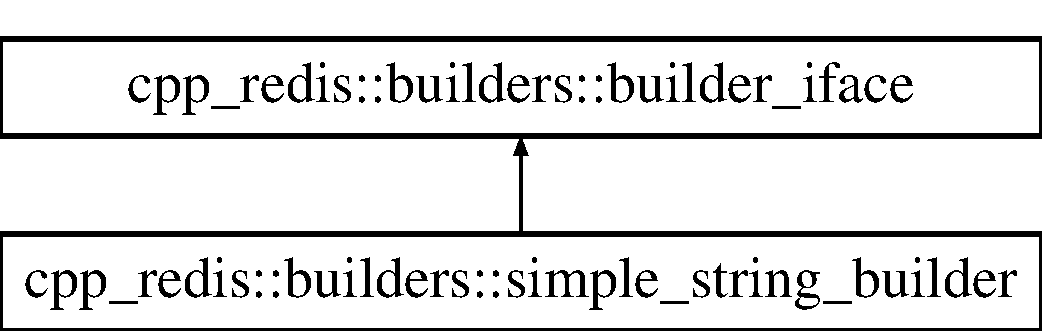
\includegraphics[height=2.000000cm]{classcpp__redis_1_1builders_1_1simple__string__builder}
\end{center}
\end{figure}
\subsection*{Public Member Functions}
\begin{DoxyCompactItemize}
\item 
\hyperlink{classcpp__redis_1_1builders_1_1simple__string__builder_a51fcb7777a78cbd3599aae8896e4d06a}{simple\+\_\+string\+\_\+builder} (void)
\begin{DoxyCompactList}\small\item\em ctor \end{DoxyCompactList}\item 
\hyperlink{classcpp__redis_1_1builders_1_1simple__string__builder_a7b4f012c532535801f9d5fddbb01d675}{$\sim$simple\+\_\+string\+\_\+builder} (void)=default
\begin{DoxyCompactList}\small\item\em dtor \end{DoxyCompactList}\item 
\hyperlink{classcpp__redis_1_1builders_1_1simple__string__builder_a0a17d659e654ee1190c635d3b3093235}{simple\+\_\+string\+\_\+builder} (const \hyperlink{classcpp__redis_1_1builders_1_1simple__string__builder}{simple\+\_\+string\+\_\+builder} \&)=delete
\begin{DoxyCompactList}\small\item\em copy ctor \end{DoxyCompactList}\item 
\hyperlink{classcpp__redis_1_1builders_1_1simple__string__builder}{simple\+\_\+string\+\_\+builder} \& \hyperlink{classcpp__redis_1_1builders_1_1simple__string__builder_afc86dd3148ef0094d08b4282f7cb597d}{operator=} (const \hyperlink{classcpp__redis_1_1builders_1_1simple__string__builder}{simple\+\_\+string\+\_\+builder} \&)=delete
\begin{DoxyCompactList}\small\item\em assignment operator \end{DoxyCompactList}\item 
\hyperlink{classcpp__redis_1_1builders_1_1builder__iface}{builder\+\_\+iface} \& \hyperlink{classcpp__redis_1_1builders_1_1simple__string__builder_a159bb512f0427c4a988742f7cd01035e}{operator$<$$<$} (std\+::string \&data)
\item 
bool \hyperlink{classcpp__redis_1_1builders_1_1simple__string__builder_ad586164caf02b3022b91789cac23a72d}{reply\+\_\+ready} (void) const
\item 
\hyperlink{classcpp__redis_1_1reply}{reply} \hyperlink{classcpp__redis_1_1builders_1_1simple__string__builder_a24ad0968d7d02172a65cf8982c540d51}{get\+\_\+reply} (void) const
\item 
const std\+::string \& \hyperlink{classcpp__redis_1_1builders_1_1simple__string__builder_a539ba8a9234269e57471f1973adc58c2}{get\+\_\+simple\+\_\+string} (void) const
\end{DoxyCompactItemize}
\subsection*{Private Attributes}
\begin{DoxyCompactItemize}
\item 
std\+::string \hyperlink{classcpp__redis_1_1builders_1_1simple__string__builder_acf61d3d6bec2cc33279f4e6ee4cd6f80}{m\+\_\+str}
\item 
bool \hyperlink{classcpp__redis_1_1builders_1_1simple__string__builder_aaf2076e8d2d7154ddc1433aff77a5013}{m\+\_\+reply\+\_\+ready}
\item 
\hyperlink{classcpp__redis_1_1reply}{reply} \hyperlink{classcpp__redis_1_1builders_1_1simple__string__builder_a8a9ee04b09475ab079db623f1d887757}{m\+\_\+reply}
\end{DoxyCompactItemize}


\subsection{Detailed Description}
builder to build redis simplestring replies 

\subsection{Constructor \& Destructor Documentation}
\mbox{\Hypertarget{classcpp__redis_1_1builders_1_1simple__string__builder_a51fcb7777a78cbd3599aae8896e4d06a}\label{classcpp__redis_1_1builders_1_1simple__string__builder_a51fcb7777a78cbd3599aae8896e4d06a}} 
\index{cpp\+\_\+redis\+::builders\+::simple\+\_\+string\+\_\+builder@{cpp\+\_\+redis\+::builders\+::simple\+\_\+string\+\_\+builder}!simple\+\_\+string\+\_\+builder@{simple\+\_\+string\+\_\+builder}}
\index{simple\+\_\+string\+\_\+builder@{simple\+\_\+string\+\_\+builder}!cpp\+\_\+redis\+::builders\+::simple\+\_\+string\+\_\+builder@{cpp\+\_\+redis\+::builders\+::simple\+\_\+string\+\_\+builder}}
\subsubsection{\texorpdfstring{simple\+\_\+string\+\_\+builder()}{simple\_string\_builder()}\hspace{0.1cm}{\footnotesize\ttfamily [1/2]}}
{\footnotesize\ttfamily cpp\+\_\+redis\+::builders\+::simple\+\_\+string\+\_\+builder\+::simple\+\_\+string\+\_\+builder (\begin{DoxyParamCaption}\item[{void}]{ }\end{DoxyParamCaption})}



ctor 

\mbox{\Hypertarget{classcpp__redis_1_1builders_1_1simple__string__builder_a7b4f012c532535801f9d5fddbb01d675}\label{classcpp__redis_1_1builders_1_1simple__string__builder_a7b4f012c532535801f9d5fddbb01d675}} 
\index{cpp\+\_\+redis\+::builders\+::simple\+\_\+string\+\_\+builder@{cpp\+\_\+redis\+::builders\+::simple\+\_\+string\+\_\+builder}!````~simple\+\_\+string\+\_\+builder@{$\sim$simple\+\_\+string\+\_\+builder}}
\index{````~simple\+\_\+string\+\_\+builder@{$\sim$simple\+\_\+string\+\_\+builder}!cpp\+\_\+redis\+::builders\+::simple\+\_\+string\+\_\+builder@{cpp\+\_\+redis\+::builders\+::simple\+\_\+string\+\_\+builder}}
\subsubsection{\texorpdfstring{$\sim$simple\+\_\+string\+\_\+builder()}{~simple\_string\_builder()}}
{\footnotesize\ttfamily cpp\+\_\+redis\+::builders\+::simple\+\_\+string\+\_\+builder\+::$\sim$simple\+\_\+string\+\_\+builder (\begin{DoxyParamCaption}\item[{void}]{ }\end{DoxyParamCaption})\hspace{0.3cm}{\ttfamily [default]}}



dtor 

\mbox{\Hypertarget{classcpp__redis_1_1builders_1_1simple__string__builder_a0a17d659e654ee1190c635d3b3093235}\label{classcpp__redis_1_1builders_1_1simple__string__builder_a0a17d659e654ee1190c635d3b3093235}} 
\index{cpp\+\_\+redis\+::builders\+::simple\+\_\+string\+\_\+builder@{cpp\+\_\+redis\+::builders\+::simple\+\_\+string\+\_\+builder}!simple\+\_\+string\+\_\+builder@{simple\+\_\+string\+\_\+builder}}
\index{simple\+\_\+string\+\_\+builder@{simple\+\_\+string\+\_\+builder}!cpp\+\_\+redis\+::builders\+::simple\+\_\+string\+\_\+builder@{cpp\+\_\+redis\+::builders\+::simple\+\_\+string\+\_\+builder}}
\subsubsection{\texorpdfstring{simple\+\_\+string\+\_\+builder()}{simple\_string\_builder()}\hspace{0.1cm}{\footnotesize\ttfamily [2/2]}}
{\footnotesize\ttfamily cpp\+\_\+redis\+::builders\+::simple\+\_\+string\+\_\+builder\+::simple\+\_\+string\+\_\+builder (\begin{DoxyParamCaption}\item[{const \hyperlink{classcpp__redis_1_1builders_1_1simple__string__builder}{simple\+\_\+string\+\_\+builder} \&}]{ }\end{DoxyParamCaption})\hspace{0.3cm}{\ttfamily [delete]}}



copy ctor 



\subsection{Member Function Documentation}
\mbox{\Hypertarget{classcpp__redis_1_1builders_1_1simple__string__builder_a24ad0968d7d02172a65cf8982c540d51}\label{classcpp__redis_1_1builders_1_1simple__string__builder_a24ad0968d7d02172a65cf8982c540d51}} 
\index{cpp\+\_\+redis\+::builders\+::simple\+\_\+string\+\_\+builder@{cpp\+\_\+redis\+::builders\+::simple\+\_\+string\+\_\+builder}!get\+\_\+reply@{get\+\_\+reply}}
\index{get\+\_\+reply@{get\+\_\+reply}!cpp\+\_\+redis\+::builders\+::simple\+\_\+string\+\_\+builder@{cpp\+\_\+redis\+::builders\+::simple\+\_\+string\+\_\+builder}}
\subsubsection{\texorpdfstring{get\+\_\+reply()}{get\_reply()}}
{\footnotesize\ttfamily \hyperlink{classcpp__redis_1_1reply}{reply} cpp\+\_\+redis\+::builders\+::simple\+\_\+string\+\_\+builder\+::get\+\_\+reply (\begin{DoxyParamCaption}\item[{void}]{ }\end{DoxyParamCaption}) const\hspace{0.3cm}{\ttfamily [virtual]}}

\begin{DoxyReturn}{Returns}
reply object 
\end{DoxyReturn}


Implements \hyperlink{classcpp__redis_1_1builders_1_1builder__iface_afd2ff2c2371c2a486116543b638b9413}{cpp\+\_\+redis\+::builders\+::builder\+\_\+iface}.

\mbox{\Hypertarget{classcpp__redis_1_1builders_1_1simple__string__builder_a539ba8a9234269e57471f1973adc58c2}\label{classcpp__redis_1_1builders_1_1simple__string__builder_a539ba8a9234269e57471f1973adc58c2}} 
\index{cpp\+\_\+redis\+::builders\+::simple\+\_\+string\+\_\+builder@{cpp\+\_\+redis\+::builders\+::simple\+\_\+string\+\_\+builder}!get\+\_\+simple\+\_\+string@{get\+\_\+simple\+\_\+string}}
\index{get\+\_\+simple\+\_\+string@{get\+\_\+simple\+\_\+string}!cpp\+\_\+redis\+::builders\+::simple\+\_\+string\+\_\+builder@{cpp\+\_\+redis\+::builders\+::simple\+\_\+string\+\_\+builder}}
\subsubsection{\texorpdfstring{get\+\_\+simple\+\_\+string()}{get\_simple\_string()}}
{\footnotesize\ttfamily const std\+::string\& cpp\+\_\+redis\+::builders\+::simple\+\_\+string\+\_\+builder\+::get\+\_\+simple\+\_\+string (\begin{DoxyParamCaption}\item[{void}]{ }\end{DoxyParamCaption}) const}

\begin{DoxyReturn}{Returns}
the parsed simple string 
\end{DoxyReturn}
\mbox{\Hypertarget{classcpp__redis_1_1builders_1_1simple__string__builder_a159bb512f0427c4a988742f7cd01035e}\label{classcpp__redis_1_1builders_1_1simple__string__builder_a159bb512f0427c4a988742f7cd01035e}} 
\index{cpp\+\_\+redis\+::builders\+::simple\+\_\+string\+\_\+builder@{cpp\+\_\+redis\+::builders\+::simple\+\_\+string\+\_\+builder}!operator$<$$<$@{operator$<$$<$}}
\index{operator$<$$<$@{operator$<$$<$}!cpp\+\_\+redis\+::builders\+::simple\+\_\+string\+\_\+builder@{cpp\+\_\+redis\+::builders\+::simple\+\_\+string\+\_\+builder}}
\subsubsection{\texorpdfstring{operator$<$$<$()}{operator<<()}}
{\footnotesize\ttfamily \hyperlink{classcpp__redis_1_1builders_1_1builder__iface}{builder\+\_\+iface}\& cpp\+\_\+redis\+::builders\+::simple\+\_\+string\+\_\+builder\+::operator$<$$<$ (\begin{DoxyParamCaption}\item[{std\+::string \&}]{data }\end{DoxyParamCaption})\hspace{0.3cm}{\ttfamily [virtual]}}

take data as parameter which is consumed to build the reply every bytes used to build the reply must be removed from the buffer passed as parameter


\begin{DoxyParams}{Parameters}
{\em data} & data to be consumed \\
\hline
\end{DoxyParams}
\begin{DoxyReturn}{Returns}
current instance 
\end{DoxyReturn}


Implements \hyperlink{classcpp__redis_1_1builders_1_1builder__iface_a9892bbc9c887c31c2742dad4476e2fa6}{cpp\+\_\+redis\+::builders\+::builder\+\_\+iface}.

\mbox{\Hypertarget{classcpp__redis_1_1builders_1_1simple__string__builder_afc86dd3148ef0094d08b4282f7cb597d}\label{classcpp__redis_1_1builders_1_1simple__string__builder_afc86dd3148ef0094d08b4282f7cb597d}} 
\index{cpp\+\_\+redis\+::builders\+::simple\+\_\+string\+\_\+builder@{cpp\+\_\+redis\+::builders\+::simple\+\_\+string\+\_\+builder}!operator=@{operator=}}
\index{operator=@{operator=}!cpp\+\_\+redis\+::builders\+::simple\+\_\+string\+\_\+builder@{cpp\+\_\+redis\+::builders\+::simple\+\_\+string\+\_\+builder}}
\subsubsection{\texorpdfstring{operator=()}{operator=()}}
{\footnotesize\ttfamily \hyperlink{classcpp__redis_1_1builders_1_1simple__string__builder}{simple\+\_\+string\+\_\+builder}\& cpp\+\_\+redis\+::builders\+::simple\+\_\+string\+\_\+builder\+::operator= (\begin{DoxyParamCaption}\item[{const \hyperlink{classcpp__redis_1_1builders_1_1simple__string__builder}{simple\+\_\+string\+\_\+builder} \&}]{ }\end{DoxyParamCaption})\hspace{0.3cm}{\ttfamily [delete]}}



assignment operator 

\mbox{\Hypertarget{classcpp__redis_1_1builders_1_1simple__string__builder_ad586164caf02b3022b91789cac23a72d}\label{classcpp__redis_1_1builders_1_1simple__string__builder_ad586164caf02b3022b91789cac23a72d}} 
\index{cpp\+\_\+redis\+::builders\+::simple\+\_\+string\+\_\+builder@{cpp\+\_\+redis\+::builders\+::simple\+\_\+string\+\_\+builder}!reply\+\_\+ready@{reply\+\_\+ready}}
\index{reply\+\_\+ready@{reply\+\_\+ready}!cpp\+\_\+redis\+::builders\+::simple\+\_\+string\+\_\+builder@{cpp\+\_\+redis\+::builders\+::simple\+\_\+string\+\_\+builder}}
\subsubsection{\texorpdfstring{reply\+\_\+ready()}{reply\_ready()}}
{\footnotesize\ttfamily bool cpp\+\_\+redis\+::builders\+::simple\+\_\+string\+\_\+builder\+::reply\+\_\+ready (\begin{DoxyParamCaption}\item[{void}]{ }\end{DoxyParamCaption}) const\hspace{0.3cm}{\ttfamily [virtual]}}

\begin{DoxyReturn}{Returns}
whether the reply could be built 
\end{DoxyReturn}


Implements \hyperlink{classcpp__redis_1_1builders_1_1builder__iface_a40db9a31d4ea1771777e74146d31e12d}{cpp\+\_\+redis\+::builders\+::builder\+\_\+iface}.



\subsection{Member Data Documentation}
\mbox{\Hypertarget{classcpp__redis_1_1builders_1_1simple__string__builder_a8a9ee04b09475ab079db623f1d887757}\label{classcpp__redis_1_1builders_1_1simple__string__builder_a8a9ee04b09475ab079db623f1d887757}} 
\index{cpp\+\_\+redis\+::builders\+::simple\+\_\+string\+\_\+builder@{cpp\+\_\+redis\+::builders\+::simple\+\_\+string\+\_\+builder}!m\+\_\+reply@{m\+\_\+reply}}
\index{m\+\_\+reply@{m\+\_\+reply}!cpp\+\_\+redis\+::builders\+::simple\+\_\+string\+\_\+builder@{cpp\+\_\+redis\+::builders\+::simple\+\_\+string\+\_\+builder}}
\subsubsection{\texorpdfstring{m\+\_\+reply}{m\_reply}}
{\footnotesize\ttfamily \hyperlink{classcpp__redis_1_1reply}{reply} cpp\+\_\+redis\+::builders\+::simple\+\_\+string\+\_\+builder\+::m\+\_\+reply\hspace{0.3cm}{\ttfamily [private]}}

reply to be built \mbox{\Hypertarget{classcpp__redis_1_1builders_1_1simple__string__builder_aaf2076e8d2d7154ddc1433aff77a5013}\label{classcpp__redis_1_1builders_1_1simple__string__builder_aaf2076e8d2d7154ddc1433aff77a5013}} 
\index{cpp\+\_\+redis\+::builders\+::simple\+\_\+string\+\_\+builder@{cpp\+\_\+redis\+::builders\+::simple\+\_\+string\+\_\+builder}!m\+\_\+reply\+\_\+ready@{m\+\_\+reply\+\_\+ready}}
\index{m\+\_\+reply\+\_\+ready@{m\+\_\+reply\+\_\+ready}!cpp\+\_\+redis\+::builders\+::simple\+\_\+string\+\_\+builder@{cpp\+\_\+redis\+::builders\+::simple\+\_\+string\+\_\+builder}}
\subsubsection{\texorpdfstring{m\+\_\+reply\+\_\+ready}{m\_reply\_ready}}
{\footnotesize\ttfamily bool cpp\+\_\+redis\+::builders\+::simple\+\_\+string\+\_\+builder\+::m\+\_\+reply\+\_\+ready\hspace{0.3cm}{\ttfamily [private]}}

whether the reply is ready or not \mbox{\Hypertarget{classcpp__redis_1_1builders_1_1simple__string__builder_acf61d3d6bec2cc33279f4e6ee4cd6f80}\label{classcpp__redis_1_1builders_1_1simple__string__builder_acf61d3d6bec2cc33279f4e6ee4cd6f80}} 
\index{cpp\+\_\+redis\+::builders\+::simple\+\_\+string\+\_\+builder@{cpp\+\_\+redis\+::builders\+::simple\+\_\+string\+\_\+builder}!m\+\_\+str@{m\+\_\+str}}
\index{m\+\_\+str@{m\+\_\+str}!cpp\+\_\+redis\+::builders\+::simple\+\_\+string\+\_\+builder@{cpp\+\_\+redis\+::builders\+::simple\+\_\+string\+\_\+builder}}
\subsubsection{\texorpdfstring{m\+\_\+str}{m\_str}}
{\footnotesize\ttfamily std\+::string cpp\+\_\+redis\+::builders\+::simple\+\_\+string\+\_\+builder\+::m\+\_\+str\hspace{0.3cm}{\ttfamily [private]}}

parsed simple string 

The documentation for this class was generated from the following file\+:\begin{DoxyCompactItemize}
\item 
includes/cpp\+\_\+redis/builders/\hyperlink{simple__string__builder_8hpp}{simple\+\_\+string\+\_\+builder.\+hpp}\end{DoxyCompactItemize}

\hypertarget{classcpp__redis_1_1subscriber}{}\section{cpp\+\_\+redis\+:\+:subscriber Class Reference}
\label{classcpp__redis_1_1subscriber}\index{cpp\+\_\+redis\+::subscriber@{cpp\+\_\+redis\+::subscriber}}


{\ttfamily \#include $<$subscriber.\+hpp$>$}

\subsection*{Classes}
\begin{DoxyCompactItemize}
\item 
struct \hyperlink{structcpp__redis_1_1subscriber_1_1callback__holder}{callback\+\_\+holder}
\end{DoxyCompactItemize}
\subsection*{Public Types}
\begin{DoxyCompactItemize}
\item 
enum \hyperlink{classcpp__redis_1_1subscriber_afc976757efd9d0ac4def6935546a2338}{connect\+\_\+state} \{ \newline
\hyperlink{classcpp__redis_1_1subscriber_afc976757efd9d0ac4def6935546a2338a41d368a58ee26891a6a586ddaaa604f8}{connect\+\_\+state\+::dropped}, 
\hyperlink{classcpp__redis_1_1subscriber_afc976757efd9d0ac4def6935546a2338aea2b2676c28c0db26d39331a336c6b92}{connect\+\_\+state\+::start}, 
\hyperlink{classcpp__redis_1_1subscriber_afc976757efd9d0ac4def6935546a2338ad98cb5df35fc9e0f42fb883d794ad12f}{connect\+\_\+state\+::sleeping}, 
\hyperlink{classcpp__redis_1_1subscriber_afc976757efd9d0ac4def6935546a2338a444bcb3a3fcf8389296c49467f27e1d6}{connect\+\_\+state\+::ok}, 
\newline
\hyperlink{classcpp__redis_1_1subscriber_afc976757efd9d0ac4def6935546a2338a26934eb377001f66e37289a5c93fe284}{connect\+\_\+state\+::failed}, 
\hyperlink{classcpp__redis_1_1subscriber_afc976757efd9d0ac4def6935546a2338a1c35224aee766403970dfaa34880ccde}{connect\+\_\+state\+::lookup\+\_\+failed}, 
\hyperlink{classcpp__redis_1_1subscriber_afc976757efd9d0ac4def6935546a2338af0a0bfe6bc7d2c58d2989034f83183e0}{connect\+\_\+state\+::stopped}
 \}
\item 
typedef std\+::function$<$ void(const std\+::string \&host, std\+::size\+\_\+t port, \hyperlink{classcpp__redis_1_1subscriber_afc976757efd9d0ac4def6935546a2338}{connect\+\_\+state} status)$>$ \hyperlink{classcpp__redis_1_1subscriber_a90f2f7d4c748c3c2e89d1e977fa6dce1}{connect\+\_\+callback\+\_\+t}
\item 
typedef std\+::function$<$ void(\hyperlink{classcpp__redis_1_1reply}{reply} \&)$>$ \hyperlink{classcpp__redis_1_1subscriber_a99d220cc662664e2399b709f61ac9581}{reply\+\_\+callback\+\_\+t}
\item 
typedef std\+::function$<$ void(const std\+::string \&, const std\+::string \&)$>$ \hyperlink{classcpp__redis_1_1subscriber_ac6ab8ebc526d784e4b79a39bbd73dca8}{subscribe\+\_\+callback\+\_\+t}
\item 
typedef std\+::function$<$ void(int64\+\_\+t)$>$ \hyperlink{classcpp__redis_1_1subscriber_a19ea39dfabeb19937a9ce4c8d21781b4}{acknowledgement\+\_\+callback\+\_\+t}
\end{DoxyCompactItemize}
\subsection*{Public Member Functions}
\begin{DoxyCompactItemize}
\item 
\hyperlink{classcpp__redis_1_1subscriber_ab7feafca57399394e3a1a0d6daf52770}{subscriber} (void)
\begin{DoxyCompactList}\small\item\em ctor \end{DoxyCompactList}\item 
\hyperlink{classcpp__redis_1_1subscriber_a66136601f44564842e2c67de2da199af}{subscriber} (const std\+::shared\+\_\+ptr$<$ \hyperlink{classcpp__redis_1_1network_1_1tcp__client__iface}{network\+::tcp\+\_\+client\+\_\+iface} $>$ \&tcp\+\_\+client)
\item 
\hyperlink{classcpp__redis_1_1subscriber_a878caeb144b11de30466a380b09abc30}{$\sim$subscriber} (void)
\begin{DoxyCompactList}\small\item\em dtor \end{DoxyCompactList}\item 
\hyperlink{classcpp__redis_1_1subscriber_af5f11532bf727eeb2d4a926bdc775cd7}{subscriber} (const \hyperlink{classcpp__redis_1_1subscriber}{subscriber} \&)=delete
\begin{DoxyCompactList}\small\item\em copy ctor \end{DoxyCompactList}\item 
\hyperlink{classcpp__redis_1_1subscriber}{subscriber} \& \hyperlink{classcpp__redis_1_1subscriber_ac60f83e6e915073bda6853baaeb39485}{operator=} (const \hyperlink{classcpp__redis_1_1subscriber}{subscriber} \&)=delete
\begin{DoxyCompactList}\small\item\em assignment operator \end{DoxyCompactList}\item 
void \hyperlink{classcpp__redis_1_1subscriber_a6ae8134a9a9b31d6f2434ec4f6e86d3a}{connect} (const std\+::string \&host=\char`\"{}127.\+0.\+0.\+1\char`\"{}, std\+::size\+\_\+t port=6379, const \hyperlink{classcpp__redis_1_1subscriber_a90f2f7d4c748c3c2e89d1e977fa6dce1}{connect\+\_\+callback\+\_\+t} \&connect\+\_\+callback=nullptr, std\+::uint32\+\_\+t timeout\+\_\+msecs=0, std\+::int32\+\_\+t max\+\_\+reconnects=0, std\+::uint32\+\_\+t reconnect\+\_\+interval\+\_\+msecs=0)
\item 
void \hyperlink{classcpp__redis_1_1subscriber_a8fb77a44a1e1f0d99dec639658e2aa7e}{connect} (const std\+::string \&name, const \hyperlink{classcpp__redis_1_1subscriber_a90f2f7d4c748c3c2e89d1e977fa6dce1}{connect\+\_\+callback\+\_\+t} \&connect\+\_\+callback=nullptr, std\+::uint32\+\_\+t timeout\+\_\+msecs=0, std\+::int32\+\_\+t max\+\_\+reconnects=0, std\+::uint32\+\_\+t reconnect\+\_\+interval\+\_\+msecs=0)
\item 
bool \hyperlink{classcpp__redis_1_1subscriber_a13ff83c3944b33851dfcf364f53b146c}{is\+\_\+connected} (void) const
\item 
void \hyperlink{classcpp__redis_1_1subscriber_aad1d0c3c6edb1522eb7b1bdb64b4705d}{disconnect} (bool wait\+\_\+for\+\_\+removal=false)
\item 
bool \hyperlink{classcpp__redis_1_1subscriber_a32eb4feb4858c972ebb9887d21cb62d7}{is\+\_\+reconnecting} (void) const
\item 
void \hyperlink{classcpp__redis_1_1subscriber_a6d5bdcf7c5a67d1b56b021bbd450a7c3}{cancel\+\_\+reconnect} (void)
\item 
\hyperlink{classcpp__redis_1_1subscriber}{subscriber} \& \hyperlink{classcpp__redis_1_1subscriber_a7b4564fc4dfe356b95aeae4fdb8071c9}{auth} (const std\+::string \&password, const \hyperlink{classcpp__redis_1_1subscriber_a99d220cc662664e2399b709f61ac9581}{reply\+\_\+callback\+\_\+t} \&reply\+\_\+callback=nullptr)
\item 
\hyperlink{classcpp__redis_1_1subscriber}{subscriber} \& \hyperlink{classcpp__redis_1_1subscriber_afee579c702182041645a3d3c55de4b9e}{subscribe} (const std\+::string \&channel, const \hyperlink{classcpp__redis_1_1subscriber_ac6ab8ebc526d784e4b79a39bbd73dca8}{subscribe\+\_\+callback\+\_\+t} \&callback, const \hyperlink{classcpp__redis_1_1subscriber_a19ea39dfabeb19937a9ce4c8d21781b4}{acknowledgement\+\_\+callback\+\_\+t} \&acknowledgement\+\_\+callback=nullptr)
\item 
\hyperlink{classcpp__redis_1_1subscriber}{subscriber} \& \hyperlink{classcpp__redis_1_1subscriber_a52605edb2a85d370680c3c9e1b84fc3b}{psubscribe} (const std\+::string \&pattern, const \hyperlink{classcpp__redis_1_1subscriber_ac6ab8ebc526d784e4b79a39bbd73dca8}{subscribe\+\_\+callback\+\_\+t} \&callback, const \hyperlink{classcpp__redis_1_1subscriber_a19ea39dfabeb19937a9ce4c8d21781b4}{acknowledgement\+\_\+callback\+\_\+t} \&acknowledgement\+\_\+callback=nullptr)
\item 
\hyperlink{classcpp__redis_1_1subscriber}{subscriber} \& \hyperlink{classcpp__redis_1_1subscriber_a08dffea41cfd5914adfa5a966e0ab292}{unsubscribe} (const std\+::string \&channel)
\item 
\hyperlink{classcpp__redis_1_1subscriber}{subscriber} \& \hyperlink{classcpp__redis_1_1subscriber_a26edc7dcf87ddc8734fac04878ca307a}{punsubscribe} (const std\+::string \&pattern)
\item 
\hyperlink{classcpp__redis_1_1subscriber}{subscriber} \& \hyperlink{classcpp__redis_1_1subscriber_abbf600802ed93b82323185eec5719ecb}{commit} (void)
\item 
void \hyperlink{classcpp__redis_1_1subscriber_a10584e201abe4e701b70d078b3a676fc}{add\+\_\+sentinel} (const std\+::string \&host, std\+::size\+\_\+t port)
\item 
void \hyperlink{classcpp__redis_1_1subscriber_ac8f371c14866842cdda7cf1ee5eee2b8}{clear\+\_\+sentinels} (void)
\end{DoxyCompactItemize}
\subsection*{Private Member Functions}
\begin{DoxyCompactItemize}
\item 
void \hyperlink{classcpp__redis_1_1subscriber_ad37cdd903672a0daa395cc3624c50ecb}{connection\+\_\+receive\+\_\+handler} (\hyperlink{classcpp__redis_1_1network_1_1redis__connection}{network\+::redis\+\_\+connection} \&connection, \hyperlink{classcpp__redis_1_1reply}{reply} \&\hyperlink{classcpp__redis_1_1reply}{reply})
\item 
void \hyperlink{classcpp__redis_1_1subscriber_a344918efce6fc6f628e13c8eceeade3a}{connection\+\_\+disconnection\+\_\+handler} (\hyperlink{classcpp__redis_1_1network_1_1redis__connection}{network\+::redis\+\_\+connection} \&connection)
\item 
void \hyperlink{classcpp__redis_1_1subscriber_ade918ef2347138492fe213450f27bcfd}{handle\+\_\+acknowledgement\+\_\+reply} (const std\+::vector$<$ \hyperlink{classcpp__redis_1_1reply}{reply} $>$ \&\hyperlink{classcpp__redis_1_1reply}{reply})
\item 
void \hyperlink{classcpp__redis_1_1subscriber_a9b8e9e1dc12493703c02f2c832bd20d9}{handle\+\_\+subscribe\+\_\+reply} (const std\+::vector$<$ \hyperlink{classcpp__redis_1_1reply}{reply} $>$ \&\hyperlink{classcpp__redis_1_1reply}{reply})
\item 
void \hyperlink{classcpp__redis_1_1subscriber_a6e67df5af6170ad55e77082f18f63d76}{handle\+\_\+psubscribe\+\_\+reply} (const std\+::vector$<$ \hyperlink{classcpp__redis_1_1reply}{reply} $>$ \&\hyperlink{classcpp__redis_1_1reply}{reply})
\item 
void \hyperlink{classcpp__redis_1_1subscriber_a8cbe2790b1e0f803f41a403ed8c66513}{call\+\_\+acknowledgement\+\_\+callback} (const std\+::string \&channel, const std\+::map$<$ std\+::string, \hyperlink{structcpp__redis_1_1subscriber_1_1callback__holder}{callback\+\_\+holder} $>$ \&channels, std\+::mutex \&channels\+\_\+mtx, int64\+\_\+t nb\+\_\+chans)
\item 
void \hyperlink{classcpp__redis_1_1subscriber_a0d5c27ee74e5422d07ce14677ae0e23b}{reconnect} (void)
\item 
void \hyperlink{classcpp__redis_1_1subscriber_acb33b48b9dfa03b4a5b60cc832b57259}{re\+\_\+auth} (void)
\item 
void \hyperlink{classcpp__redis_1_1subscriber_ac38ffc11fb8e67159a7ffa924a6bb8a6}{re\+\_\+subscribe} (void)
\item 
bool \hyperlink{classcpp__redis_1_1subscriber_a87b9daaeed9872a0bc65438729b1211e}{should\+\_\+reconnect} (void) const
\item 
void \hyperlink{classcpp__redis_1_1subscriber_aa4a227745820990bfed151f51376ac54}{sleep\+\_\+before\+\_\+next\+\_\+reconnect\+\_\+attempt} (void)
\item 
void \hyperlink{classcpp__redis_1_1subscriber_a1be9e272e3b9d382e9b6c75c0c4bce70}{clear\+\_\+subscriptions} (void)
\item 
void \hyperlink{classcpp__redis_1_1subscriber_adc7f57c1c2cba9b213ce251b2b736550}{unprotected\+\_\+subscribe} (const std\+::string \&channel, const \hyperlink{classcpp__redis_1_1subscriber_ac6ab8ebc526d784e4b79a39bbd73dca8}{subscribe\+\_\+callback\+\_\+t} \&callback, const \hyperlink{classcpp__redis_1_1subscriber_a19ea39dfabeb19937a9ce4c8d21781b4}{acknowledgement\+\_\+callback\+\_\+t} \&acknowledgement\+\_\+callback)
\item 
void \hyperlink{classcpp__redis_1_1subscriber_a4c711c3fda605cb286f14bb25b205b7d}{unprotected\+\_\+psubscribe} (const std\+::string \&pattern, const \hyperlink{classcpp__redis_1_1subscriber_ac6ab8ebc526d784e4b79a39bbd73dca8}{subscribe\+\_\+callback\+\_\+t} \&callback, const \hyperlink{classcpp__redis_1_1subscriber_a19ea39dfabeb19937a9ce4c8d21781b4}{acknowledgement\+\_\+callback\+\_\+t} \&acknowledgement\+\_\+callback)
\end{DoxyCompactItemize}
\subsection*{Private Attributes}
\begin{DoxyCompactItemize}
\item 
std\+::string \hyperlink{classcpp__redis_1_1subscriber_ab3001cb0e748940490039b59efc5be7d}{m\+\_\+redis\+\_\+server}
\item 
std\+::size\+\_\+t \hyperlink{classcpp__redis_1_1subscriber_a606e99982af301b722cc1ebe8c1889bc}{m\+\_\+redis\+\_\+port} = 0
\item 
std\+::string \hyperlink{classcpp__redis_1_1subscriber_a79e64728d9f6094fdd5c24418b889f19}{m\+\_\+master\+\_\+name}
\item 
std\+::string \hyperlink{classcpp__redis_1_1subscriber_a05f90439d1da469a1184651eea89c015}{m\+\_\+password}
\item 
\hyperlink{classcpp__redis_1_1network_1_1redis__connection}{network\+::redis\+\_\+connection} \hyperlink{classcpp__redis_1_1subscriber_ac982bd5661f59b8e2021dbdb80615e38}{m\+\_\+client}
\item 
\hyperlink{classcpp__redis_1_1sentinel}{cpp\+\_\+redis\+::sentinel} \hyperlink{classcpp__redis_1_1subscriber_a74ea9dc2c41fa4bc3b19f6ae2a3c2513}{m\+\_\+sentinel}
\item 
std\+::uint32\+\_\+t \hyperlink{classcpp__redis_1_1subscriber_a2fd648e01a4b88d63b6b977e0b694fa5}{m\+\_\+connect\+\_\+timeout\+\_\+msecs} = 0
\item 
std\+::int32\+\_\+t \hyperlink{classcpp__redis_1_1subscriber_a8c22f20f5a196eb72233d203b102bf3c}{m\+\_\+max\+\_\+reconnects} = 0
\item 
std\+::uint32\+\_\+t \hyperlink{classcpp__redis_1_1subscriber_a61fb1560948d3ddaff3b322c30e7a8a7}{m\+\_\+reconnect\+\_\+interval\+\_\+msecs} = 0
\item 
std\+::atomic\+\_\+bool \hyperlink{classcpp__redis_1_1subscriber_a71517f71ac616e52b48e371be291665b}{m\+\_\+reconnecting} = A\+T\+O\+M\+I\+C\+\_\+\+V\+A\+R\+\_\+\+I\+N\+IT(false)
\item 
std\+::atomic\+\_\+bool \hyperlink{classcpp__redis_1_1subscriber_a66dd15a4eb08cf3ed7e926a83b10cc9f}{m\+\_\+cancel} = A\+T\+O\+M\+I\+C\+\_\+\+V\+A\+R\+\_\+\+I\+N\+IT(false)
\item 
std\+::map$<$ std\+::string, \hyperlink{structcpp__redis_1_1subscriber_1_1callback__holder}{callback\+\_\+holder} $>$ \hyperlink{classcpp__redis_1_1subscriber_aa0e98504b640b44f23577ed2f8e30f74}{m\+\_\+subscribed\+\_\+channels}
\item 
std\+::map$<$ std\+::string, \hyperlink{structcpp__redis_1_1subscriber_1_1callback__holder}{callback\+\_\+holder} $>$ \hyperlink{classcpp__redis_1_1subscriber_a5fa674196428e6f41f808a2f9ff7ec39}{m\+\_\+psubscribed\+\_\+channels}
\item 
\hyperlink{classcpp__redis_1_1subscriber_a90f2f7d4c748c3c2e89d1e977fa6dce1}{connect\+\_\+callback\+\_\+t} \hyperlink{classcpp__redis_1_1subscriber_a39521d60ac80bc449567125e3c509a60}{m\+\_\+connect\+\_\+callback}
\item 
std\+::mutex \hyperlink{classcpp__redis_1_1subscriber_ac2841588b66c32f9cf306672013f3300}{m\+\_\+psubscribed\+\_\+channels\+\_\+mutex}
\item 
std\+::mutex \hyperlink{classcpp__redis_1_1subscriber_ae46b99f9ff06e2a05daca6273ffbb155}{m\+\_\+subscribed\+\_\+channels\+\_\+mutex}
\item 
\hyperlink{classcpp__redis_1_1subscriber_a99d220cc662664e2399b709f61ac9581}{reply\+\_\+callback\+\_\+t} \hyperlink{classcpp__redis_1_1subscriber_a045f1c4e84a7384565deb2d8e7023dfd}{m\+\_\+auth\+\_\+reply\+\_\+callback}
\end{DoxyCompactItemize}


\subsection{Member Typedef Documentation}
\mbox{\Hypertarget{classcpp__redis_1_1subscriber_a19ea39dfabeb19937a9ce4c8d21781b4}\label{classcpp__redis_1_1subscriber_a19ea39dfabeb19937a9ce4c8d21781b4}} 
\index{cpp\+\_\+redis\+::subscriber@{cpp\+\_\+redis\+::subscriber}!acknowledgement\+\_\+callback\+\_\+t@{acknowledgement\+\_\+callback\+\_\+t}}
\index{acknowledgement\+\_\+callback\+\_\+t@{acknowledgement\+\_\+callback\+\_\+t}!cpp\+\_\+redis\+::subscriber@{cpp\+\_\+redis\+::subscriber}}
\subsubsection{\texorpdfstring{acknowledgement\+\_\+callback\+\_\+t}{acknowledgement\_callback\_t}}
{\footnotesize\ttfamily typedef std\+::function$<$void(int64\+\_\+t)$>$ \hyperlink{classcpp__redis_1_1subscriber_a19ea39dfabeb19937a9ce4c8d21781b4}{cpp\+\_\+redis\+::subscriber\+::acknowledgement\+\_\+callback\+\_\+t}}

acknowledgement callback called whenever a subscribe completes takes as parameter the int returned by the redis server (usually the number of channels you are subscribed to) \mbox{\Hypertarget{classcpp__redis_1_1subscriber_a90f2f7d4c748c3c2e89d1e977fa6dce1}\label{classcpp__redis_1_1subscriber_a90f2f7d4c748c3c2e89d1e977fa6dce1}} 
\index{cpp\+\_\+redis\+::subscriber@{cpp\+\_\+redis\+::subscriber}!connect\+\_\+callback\+\_\+t@{connect\+\_\+callback\+\_\+t}}
\index{connect\+\_\+callback\+\_\+t@{connect\+\_\+callback\+\_\+t}!cpp\+\_\+redis\+::subscriber@{cpp\+\_\+redis\+::subscriber}}
\subsubsection{\texorpdfstring{connect\+\_\+callback\+\_\+t}{connect\_callback\_t}}
{\footnotesize\ttfamily typedef std\+::function$<$void(const std\+::string\& host, std\+::size\+\_\+t port, \hyperlink{classcpp__redis_1_1subscriber_afc976757efd9d0ac4def6935546a2338}{connect\+\_\+state} status)$>$ \hyperlink{classcpp__redis_1_1subscriber_a90f2f7d4c748c3c2e89d1e977fa6dce1}{cpp\+\_\+redis\+::subscriber\+::connect\+\_\+callback\+\_\+t}}

connect handler, called whenever a new connection even occurred \mbox{\Hypertarget{classcpp__redis_1_1subscriber_a99d220cc662664e2399b709f61ac9581}\label{classcpp__redis_1_1subscriber_a99d220cc662664e2399b709f61ac9581}} 
\index{cpp\+\_\+redis\+::subscriber@{cpp\+\_\+redis\+::subscriber}!reply\+\_\+callback\+\_\+t@{reply\+\_\+callback\+\_\+t}}
\index{reply\+\_\+callback\+\_\+t@{reply\+\_\+callback\+\_\+t}!cpp\+\_\+redis\+::subscriber@{cpp\+\_\+redis\+::subscriber}}
\subsubsection{\texorpdfstring{reply\+\_\+callback\+\_\+t}{reply\_callback\_t}}
{\footnotesize\ttfamily typedef std\+::function$<$void(\hyperlink{classcpp__redis_1_1reply}{reply}\&)$>$ \hyperlink{classcpp__redis_1_1subscriber_a99d220cc662664e2399b709f61ac9581}{cpp\+\_\+redis\+::subscriber\+::reply\+\_\+callback\+\_\+t}}

reply callback called whenever a reply is received takes as parameter the received reply \mbox{\Hypertarget{classcpp__redis_1_1subscriber_ac6ab8ebc526d784e4b79a39bbd73dca8}\label{classcpp__redis_1_1subscriber_ac6ab8ebc526d784e4b79a39bbd73dca8}} 
\index{cpp\+\_\+redis\+::subscriber@{cpp\+\_\+redis\+::subscriber}!subscribe\+\_\+callback\+\_\+t@{subscribe\+\_\+callback\+\_\+t}}
\index{subscribe\+\_\+callback\+\_\+t@{subscribe\+\_\+callback\+\_\+t}!cpp\+\_\+redis\+::subscriber@{cpp\+\_\+redis\+::subscriber}}
\subsubsection{\texorpdfstring{subscribe\+\_\+callback\+\_\+t}{subscribe\_callback\_t}}
{\footnotesize\ttfamily typedef std\+::function$<$void(const std\+::string\&, const std\+::string\&)$>$ \hyperlink{classcpp__redis_1_1subscriber_ac6ab8ebc526d784e4b79a39bbd73dca8}{cpp\+\_\+redis\+::subscriber\+::subscribe\+\_\+callback\+\_\+t}}

subscribe callback, called whenever a new message is published on a subscribed channel takes as parameter the channel and the message 

\subsection{Member Enumeration Documentation}
\mbox{\Hypertarget{classcpp__redis_1_1subscriber_afc976757efd9d0ac4def6935546a2338}\label{classcpp__redis_1_1subscriber_afc976757efd9d0ac4def6935546a2338}} 
\index{cpp\+\_\+redis\+::subscriber@{cpp\+\_\+redis\+::subscriber}!connect\+\_\+state@{connect\+\_\+state}}
\index{connect\+\_\+state@{connect\+\_\+state}!cpp\+\_\+redis\+::subscriber@{cpp\+\_\+redis\+::subscriber}}
\subsubsection{\texorpdfstring{connect\+\_\+state}{connect\_state}}
{\footnotesize\ttfamily enum \hyperlink{classcpp__redis_1_1subscriber_afc976757efd9d0ac4def6935546a2338}{cpp\+\_\+redis\+::subscriber\+::connect\+\_\+state}\hspace{0.3cm}{\ttfamily [strong]}}

high availability (re)connection states
\begin{DoxyItemize}
\item dropped\+: connection has dropped
\item start\+: attemp of connection has started
\item sleeping\+: sleep between two attemps
\item ok\+: connected
\item failed\+: failed to connect
\item lookup failed\+: failed to retrieve master sentinel
\item stopped\+: stop to try to reconnect 
\end{DoxyItemize}\begin{DoxyEnumFields}{Enumerator}
\raisebox{\heightof{T}}[0pt][0pt]{\index{dropped@{dropped}!cpp\+\_\+redis\+::subscriber@{cpp\+\_\+redis\+::subscriber}}\index{cpp\+\_\+redis\+::subscriber@{cpp\+\_\+redis\+::subscriber}!dropped@{dropped}}}\mbox{\Hypertarget{classcpp__redis_1_1subscriber_afc976757efd9d0ac4def6935546a2338a41d368a58ee26891a6a586ddaaa604f8}\label{classcpp__redis_1_1subscriber_afc976757efd9d0ac4def6935546a2338a41d368a58ee26891a6a586ddaaa604f8}} 
dropped&\\
\hline

\raisebox{\heightof{T}}[0pt][0pt]{\index{start@{start}!cpp\+\_\+redis\+::subscriber@{cpp\+\_\+redis\+::subscriber}}\index{cpp\+\_\+redis\+::subscriber@{cpp\+\_\+redis\+::subscriber}!start@{start}}}\mbox{\Hypertarget{classcpp__redis_1_1subscriber_afc976757efd9d0ac4def6935546a2338aea2b2676c28c0db26d39331a336c6b92}\label{classcpp__redis_1_1subscriber_afc976757efd9d0ac4def6935546a2338aea2b2676c28c0db26d39331a336c6b92}} 
start&\\
\hline

\raisebox{\heightof{T}}[0pt][0pt]{\index{sleeping@{sleeping}!cpp\+\_\+redis\+::subscriber@{cpp\+\_\+redis\+::subscriber}}\index{cpp\+\_\+redis\+::subscriber@{cpp\+\_\+redis\+::subscriber}!sleeping@{sleeping}}}\mbox{\Hypertarget{classcpp__redis_1_1subscriber_afc976757efd9d0ac4def6935546a2338ad98cb5df35fc9e0f42fb883d794ad12f}\label{classcpp__redis_1_1subscriber_afc976757efd9d0ac4def6935546a2338ad98cb5df35fc9e0f42fb883d794ad12f}} 
sleeping&\\
\hline

\raisebox{\heightof{T}}[0pt][0pt]{\index{ok@{ok}!cpp\+\_\+redis\+::subscriber@{cpp\+\_\+redis\+::subscriber}}\index{cpp\+\_\+redis\+::subscriber@{cpp\+\_\+redis\+::subscriber}!ok@{ok}}}\mbox{\Hypertarget{classcpp__redis_1_1subscriber_afc976757efd9d0ac4def6935546a2338a444bcb3a3fcf8389296c49467f27e1d6}\label{classcpp__redis_1_1subscriber_afc976757efd9d0ac4def6935546a2338a444bcb3a3fcf8389296c49467f27e1d6}} 
ok&\\
\hline

\raisebox{\heightof{T}}[0pt][0pt]{\index{failed@{failed}!cpp\+\_\+redis\+::subscriber@{cpp\+\_\+redis\+::subscriber}}\index{cpp\+\_\+redis\+::subscriber@{cpp\+\_\+redis\+::subscriber}!failed@{failed}}}\mbox{\Hypertarget{classcpp__redis_1_1subscriber_afc976757efd9d0ac4def6935546a2338a26934eb377001f66e37289a5c93fe284}\label{classcpp__redis_1_1subscriber_afc976757efd9d0ac4def6935546a2338a26934eb377001f66e37289a5c93fe284}} 
failed&\\
\hline

\raisebox{\heightof{T}}[0pt][0pt]{\index{lookup\+\_\+failed@{lookup\+\_\+failed}!cpp\+\_\+redis\+::subscriber@{cpp\+\_\+redis\+::subscriber}}\index{cpp\+\_\+redis\+::subscriber@{cpp\+\_\+redis\+::subscriber}!lookup\+\_\+failed@{lookup\+\_\+failed}}}\mbox{\Hypertarget{classcpp__redis_1_1subscriber_afc976757efd9d0ac4def6935546a2338a1c35224aee766403970dfaa34880ccde}\label{classcpp__redis_1_1subscriber_afc976757efd9d0ac4def6935546a2338a1c35224aee766403970dfaa34880ccde}} 
lookup\+\_\+failed&\\
\hline

\raisebox{\heightof{T}}[0pt][0pt]{\index{stopped@{stopped}!cpp\+\_\+redis\+::subscriber@{cpp\+\_\+redis\+::subscriber}}\index{cpp\+\_\+redis\+::subscriber@{cpp\+\_\+redis\+::subscriber}!stopped@{stopped}}}\mbox{\Hypertarget{classcpp__redis_1_1subscriber_afc976757efd9d0ac4def6935546a2338af0a0bfe6bc7d2c58d2989034f83183e0}\label{classcpp__redis_1_1subscriber_afc976757efd9d0ac4def6935546a2338af0a0bfe6bc7d2c58d2989034f83183e0}} 
stopped&\\
\hline

\end{DoxyEnumFields}


\subsection{Constructor \& Destructor Documentation}
\mbox{\Hypertarget{classcpp__redis_1_1subscriber_ab7feafca57399394e3a1a0d6daf52770}\label{classcpp__redis_1_1subscriber_ab7feafca57399394e3a1a0d6daf52770}} 
\index{cpp\+\_\+redis\+::subscriber@{cpp\+\_\+redis\+::subscriber}!subscriber@{subscriber}}
\index{subscriber@{subscriber}!cpp\+\_\+redis\+::subscriber@{cpp\+\_\+redis\+::subscriber}}
\subsubsection{\texorpdfstring{subscriber()}{subscriber()}\hspace{0.1cm}{\footnotesize\ttfamily [1/3]}}
{\footnotesize\ttfamily cpp\+\_\+redis\+::subscriber\+::subscriber (\begin{DoxyParamCaption}\item[{void}]{ }\end{DoxyParamCaption})}



ctor 

\mbox{\Hypertarget{classcpp__redis_1_1subscriber_a66136601f44564842e2c67de2da199af}\label{classcpp__redis_1_1subscriber_a66136601f44564842e2c67de2da199af}} 
\index{cpp\+\_\+redis\+::subscriber@{cpp\+\_\+redis\+::subscriber}!subscriber@{subscriber}}
\index{subscriber@{subscriber}!cpp\+\_\+redis\+::subscriber@{cpp\+\_\+redis\+::subscriber}}
\subsubsection{\texorpdfstring{subscriber()}{subscriber()}\hspace{0.1cm}{\footnotesize\ttfamily [2/3]}}
{\footnotesize\ttfamily cpp\+\_\+redis\+::subscriber\+::subscriber (\begin{DoxyParamCaption}\item[{const std\+::shared\+\_\+ptr$<$ \hyperlink{classcpp__redis_1_1network_1_1tcp__client__iface}{network\+::tcp\+\_\+client\+\_\+iface} $>$ \&}]{tcp\+\_\+client }\end{DoxyParamCaption})\hspace{0.3cm}{\ttfamily [explicit]}}

custom ctor to specify custom tcp\+\_\+client


\begin{DoxyParams}{Parameters}
{\em tcp\+\_\+client} & tcp client to be used for network communications \\
\hline
\end{DoxyParams}
\mbox{\Hypertarget{classcpp__redis_1_1subscriber_a878caeb144b11de30466a380b09abc30}\label{classcpp__redis_1_1subscriber_a878caeb144b11de30466a380b09abc30}} 
\index{cpp\+\_\+redis\+::subscriber@{cpp\+\_\+redis\+::subscriber}!````~subscriber@{$\sim$subscriber}}
\index{````~subscriber@{$\sim$subscriber}!cpp\+\_\+redis\+::subscriber@{cpp\+\_\+redis\+::subscriber}}
\subsubsection{\texorpdfstring{$\sim$subscriber()}{~subscriber()}}
{\footnotesize\ttfamily cpp\+\_\+redis\+::subscriber\+::$\sim$subscriber (\begin{DoxyParamCaption}\item[{void}]{ }\end{DoxyParamCaption})}



dtor 

\mbox{\Hypertarget{classcpp__redis_1_1subscriber_af5f11532bf727eeb2d4a926bdc775cd7}\label{classcpp__redis_1_1subscriber_af5f11532bf727eeb2d4a926bdc775cd7}} 
\index{cpp\+\_\+redis\+::subscriber@{cpp\+\_\+redis\+::subscriber}!subscriber@{subscriber}}
\index{subscriber@{subscriber}!cpp\+\_\+redis\+::subscriber@{cpp\+\_\+redis\+::subscriber}}
\subsubsection{\texorpdfstring{subscriber()}{subscriber()}\hspace{0.1cm}{\footnotesize\ttfamily [3/3]}}
{\footnotesize\ttfamily cpp\+\_\+redis\+::subscriber\+::subscriber (\begin{DoxyParamCaption}\item[{const \hyperlink{classcpp__redis_1_1subscriber}{subscriber} \&}]{ }\end{DoxyParamCaption})\hspace{0.3cm}{\ttfamily [delete]}}



copy ctor 



\subsection{Member Function Documentation}
\mbox{\Hypertarget{classcpp__redis_1_1subscriber_a10584e201abe4e701b70d078b3a676fc}\label{classcpp__redis_1_1subscriber_a10584e201abe4e701b70d078b3a676fc}} 
\index{cpp\+\_\+redis\+::subscriber@{cpp\+\_\+redis\+::subscriber}!add\+\_\+sentinel@{add\+\_\+sentinel}}
\index{add\+\_\+sentinel@{add\+\_\+sentinel}!cpp\+\_\+redis\+::subscriber@{cpp\+\_\+redis\+::subscriber}}
\subsubsection{\texorpdfstring{add\+\_\+sentinel()}{add\_sentinel()}}
{\footnotesize\ttfamily void cpp\+\_\+redis\+::subscriber\+::add\+\_\+sentinel (\begin{DoxyParamCaption}\item[{const std\+::string \&}]{host,  }\item[{std\+::size\+\_\+t}]{port }\end{DoxyParamCaption})}

add a sentinel definition. Required for \hyperlink{classcpp__redis_1_1subscriber_a6ae8134a9a9b31d6f2434ec4f6e86d3a}{connect()} or get\+\_\+master\+\_\+addr\+\_\+by\+\_\+name() when autoconnect is enabled.


\begin{DoxyParams}{Parameters}
{\em host} & sentinel host \\
\hline
{\em port} & sentinel port \\
\hline
\end{DoxyParams}
\mbox{\Hypertarget{classcpp__redis_1_1subscriber_a7b4564fc4dfe356b95aeae4fdb8071c9}\label{classcpp__redis_1_1subscriber_a7b4564fc4dfe356b95aeae4fdb8071c9}} 
\index{cpp\+\_\+redis\+::subscriber@{cpp\+\_\+redis\+::subscriber}!auth@{auth}}
\index{auth@{auth}!cpp\+\_\+redis\+::subscriber@{cpp\+\_\+redis\+::subscriber}}
\subsubsection{\texorpdfstring{auth()}{auth()}}
{\footnotesize\ttfamily \hyperlink{classcpp__redis_1_1subscriber}{subscriber}\& cpp\+\_\+redis\+::subscriber\+::auth (\begin{DoxyParamCaption}\item[{const std\+::string \&}]{password,  }\item[{const \hyperlink{classcpp__redis_1_1subscriber_a99d220cc662664e2399b709f61ac9581}{reply\+\_\+callback\+\_\+t} \&}]{reply\+\_\+callback = {\ttfamily nullptr} }\end{DoxyParamCaption})}

ability to authenticate on the redis server if necessary this method should not be called repeatedly as the storage of reply\+\_\+callback is N\+OT threadsafe (only one reply callback is stored for the subscriber client) calling repeatedly \hyperlink{classcpp__redis_1_1subscriber_a7b4564fc4dfe356b95aeae4fdb8071c9}{auth()} is undefined concerning the execution of the associated callbacks


\begin{DoxyParams}{Parameters}
{\em password} & password to be used for authentication \\
\hline
{\em reply\+\_\+callback} & callback to be called on auth completion (nullable) \\
\hline
\end{DoxyParams}
\begin{DoxyReturn}{Returns}
current instance 
\end{DoxyReturn}
\mbox{\Hypertarget{classcpp__redis_1_1subscriber_a8cbe2790b1e0f803f41a403ed8c66513}\label{classcpp__redis_1_1subscriber_a8cbe2790b1e0f803f41a403ed8c66513}} 
\index{cpp\+\_\+redis\+::subscriber@{cpp\+\_\+redis\+::subscriber}!call\+\_\+acknowledgement\+\_\+callback@{call\+\_\+acknowledgement\+\_\+callback}}
\index{call\+\_\+acknowledgement\+\_\+callback@{call\+\_\+acknowledgement\+\_\+callback}!cpp\+\_\+redis\+::subscriber@{cpp\+\_\+redis\+::subscriber}}
\subsubsection{\texorpdfstring{call\+\_\+acknowledgement\+\_\+callback()}{call\_acknowledgement\_callback()}}
{\footnotesize\ttfamily void cpp\+\_\+redis\+::subscriber\+::call\+\_\+acknowledgement\+\_\+callback (\begin{DoxyParamCaption}\item[{const std\+::string \&}]{channel,  }\item[{const std\+::map$<$ std\+::string, \hyperlink{structcpp__redis_1_1subscriber_1_1callback__holder}{callback\+\_\+holder} $>$ \&}]{channels,  }\item[{std\+::mutex \&}]{channels\+\_\+mtx,  }\item[{int64\+\_\+t}]{nb\+\_\+chans }\end{DoxyParamCaption})\hspace{0.3cm}{\ttfamily [private]}}

find channel or pattern that is associated to the reply and call its ack callback


\begin{DoxyParams}{Parameters}
{\em channel} & channel or pattern that caused the issuance of this reply \\
\hline
{\em channels} & list of channels or patterns to be searched for the received channel \\
\hline
{\em channels\+\_\+mtx} & channels or patterns mtx to be locked for race condition \\
\hline
{\em nb\+\_\+chans} & redis server ack reply \\
\hline
\end{DoxyParams}
\mbox{\Hypertarget{classcpp__redis_1_1subscriber_a6d5bdcf7c5a67d1b56b021bbd450a7c3}\label{classcpp__redis_1_1subscriber_a6d5bdcf7c5a67d1b56b021bbd450a7c3}} 
\index{cpp\+\_\+redis\+::subscriber@{cpp\+\_\+redis\+::subscriber}!cancel\+\_\+reconnect@{cancel\+\_\+reconnect}}
\index{cancel\+\_\+reconnect@{cancel\+\_\+reconnect}!cpp\+\_\+redis\+::subscriber@{cpp\+\_\+redis\+::subscriber}}
\subsubsection{\texorpdfstring{cancel\+\_\+reconnect()}{cancel\_reconnect()}}
{\footnotesize\ttfamily void cpp\+\_\+redis\+::subscriber\+::cancel\+\_\+reconnect (\begin{DoxyParamCaption}\item[{void}]{ }\end{DoxyParamCaption})}

stop any reconnect in progress \mbox{\Hypertarget{classcpp__redis_1_1subscriber_ac8f371c14866842cdda7cf1ee5eee2b8}\label{classcpp__redis_1_1subscriber_ac8f371c14866842cdda7cf1ee5eee2b8}} 
\index{cpp\+\_\+redis\+::subscriber@{cpp\+\_\+redis\+::subscriber}!clear\+\_\+sentinels@{clear\+\_\+sentinels}}
\index{clear\+\_\+sentinels@{clear\+\_\+sentinels}!cpp\+\_\+redis\+::subscriber@{cpp\+\_\+redis\+::subscriber}}
\subsubsection{\texorpdfstring{clear\+\_\+sentinels()}{clear\_sentinels()}}
{\footnotesize\ttfamily void cpp\+\_\+redis\+::subscriber\+::clear\+\_\+sentinels (\begin{DoxyParamCaption}\item[{void}]{ }\end{DoxyParamCaption})}

clear all existing sentinels. \mbox{\Hypertarget{classcpp__redis_1_1subscriber_a1be9e272e3b9d382e9b6c75c0c4bce70}\label{classcpp__redis_1_1subscriber_a1be9e272e3b9d382e9b6c75c0c4bce70}} 
\index{cpp\+\_\+redis\+::subscriber@{cpp\+\_\+redis\+::subscriber}!clear\+\_\+subscriptions@{clear\+\_\+subscriptions}}
\index{clear\+\_\+subscriptions@{clear\+\_\+subscriptions}!cpp\+\_\+redis\+::subscriber@{cpp\+\_\+redis\+::subscriber}}
\subsubsection{\texorpdfstring{clear\+\_\+subscriptions()}{clear\_subscriptions()}}
{\footnotesize\ttfamily void cpp\+\_\+redis\+::subscriber\+::clear\+\_\+subscriptions (\begin{DoxyParamCaption}\item[{void}]{ }\end{DoxyParamCaption})\hspace{0.3cm}{\ttfamily [private]}}

clear all subscriptions (dirty way, no unsub/punsub commands send\+: mostly used for cleaning in disconnection condition) \mbox{\Hypertarget{classcpp__redis_1_1subscriber_abbf600802ed93b82323185eec5719ecb}\label{classcpp__redis_1_1subscriber_abbf600802ed93b82323185eec5719ecb}} 
\index{cpp\+\_\+redis\+::subscriber@{cpp\+\_\+redis\+::subscriber}!commit@{commit}}
\index{commit@{commit}!cpp\+\_\+redis\+::subscriber@{cpp\+\_\+redis\+::subscriber}}
\subsubsection{\texorpdfstring{commit()}{commit()}}
{\footnotesize\ttfamily \hyperlink{classcpp__redis_1_1subscriber}{subscriber}\& cpp\+\_\+redis\+::subscriber\+::commit (\begin{DoxyParamCaption}\item[{void}]{ }\end{DoxyParamCaption})}

commit pipelined transaction that is, send to the network all commands pipelined by calling send() / \hyperlink{classcpp__redis_1_1subscriber_afee579c702182041645a3d3c55de4b9e}{subscribe()} / ...

\begin{DoxyReturn}{Returns}
current instance 
\end{DoxyReturn}
\mbox{\Hypertarget{classcpp__redis_1_1subscriber_a6ae8134a9a9b31d6f2434ec4f6e86d3a}\label{classcpp__redis_1_1subscriber_a6ae8134a9a9b31d6f2434ec4f6e86d3a}} 
\index{cpp\+\_\+redis\+::subscriber@{cpp\+\_\+redis\+::subscriber}!connect@{connect}}
\index{connect@{connect}!cpp\+\_\+redis\+::subscriber@{cpp\+\_\+redis\+::subscriber}}
\subsubsection{\texorpdfstring{connect()}{connect()}\hspace{0.1cm}{\footnotesize\ttfamily [1/2]}}
{\footnotesize\ttfamily void cpp\+\_\+redis\+::subscriber\+::connect (\begin{DoxyParamCaption}\item[{const std\+::string \&}]{host = {\ttfamily \char`\"{}127.0.0.1\char`\"{}},  }\item[{std\+::size\+\_\+t}]{port = {\ttfamily 6379},  }\item[{const \hyperlink{classcpp__redis_1_1subscriber_a90f2f7d4c748c3c2e89d1e977fa6dce1}{connect\+\_\+callback\+\_\+t} \&}]{connect\+\_\+callback = {\ttfamily nullptr},  }\item[{std\+::uint32\+\_\+t}]{timeout\+\_\+msecs = {\ttfamily 0},  }\item[{std\+::int32\+\_\+t}]{max\+\_\+reconnects = {\ttfamily 0},  }\item[{std\+::uint32\+\_\+t}]{reconnect\+\_\+interval\+\_\+msecs = {\ttfamily 0} }\end{DoxyParamCaption})}

Connect to redis server


\begin{DoxyParams}{Parameters}
{\em host} & host to be connected to \\
\hline
{\em port} & port to be connected to \\
\hline
{\em connect\+\_\+callback} & connect handler to be called on connect events (may be null) \\
\hline
{\em timeout\+\_\+msecs} & maximum time to connect \\
\hline
{\em max\+\_\+reconnects} & maximum attemps of reconnection if connection dropped \\
\hline
{\em reconnect\+\_\+interval\+\_\+msecs} & time between two attemps of reconnection \\
\hline
\end{DoxyParams}
\mbox{\Hypertarget{classcpp__redis_1_1subscriber_a8fb77a44a1e1f0d99dec639658e2aa7e}\label{classcpp__redis_1_1subscriber_a8fb77a44a1e1f0d99dec639658e2aa7e}} 
\index{cpp\+\_\+redis\+::subscriber@{cpp\+\_\+redis\+::subscriber}!connect@{connect}}
\index{connect@{connect}!cpp\+\_\+redis\+::subscriber@{cpp\+\_\+redis\+::subscriber}}
\subsubsection{\texorpdfstring{connect()}{connect()}\hspace{0.1cm}{\footnotesize\ttfamily [2/2]}}
{\footnotesize\ttfamily void cpp\+\_\+redis\+::subscriber\+::connect (\begin{DoxyParamCaption}\item[{const std\+::string \&}]{name,  }\item[{const \hyperlink{classcpp__redis_1_1subscriber_a90f2f7d4c748c3c2e89d1e977fa6dce1}{connect\+\_\+callback\+\_\+t} \&}]{connect\+\_\+callback = {\ttfamily nullptr},  }\item[{std\+::uint32\+\_\+t}]{timeout\+\_\+msecs = {\ttfamily 0},  }\item[{std\+::int32\+\_\+t}]{max\+\_\+reconnects = {\ttfamily 0},  }\item[{std\+::uint32\+\_\+t}]{reconnect\+\_\+interval\+\_\+msecs = {\ttfamily 0} }\end{DoxyParamCaption})}

Connect to redis server


\begin{DoxyParams}{Parameters}
{\em name} & sentinel name \\
\hline
{\em connect\+\_\+callback} & connect handler to be called on connect events (may be null) \\
\hline
{\em timeout\+\_\+msecs} & maximum time to connect \\
\hline
{\em max\+\_\+reconnects} & maximum attemps of reconnection if connection dropped \\
\hline
{\em reconnect\+\_\+interval\+\_\+msecs} & time between two attemps of reconnection \\
\hline
\end{DoxyParams}
\mbox{\Hypertarget{classcpp__redis_1_1subscriber_a344918efce6fc6f628e13c8eceeade3a}\label{classcpp__redis_1_1subscriber_a344918efce6fc6f628e13c8eceeade3a}} 
\index{cpp\+\_\+redis\+::subscriber@{cpp\+\_\+redis\+::subscriber}!connection\+\_\+disconnection\+\_\+handler@{connection\+\_\+disconnection\+\_\+handler}}
\index{connection\+\_\+disconnection\+\_\+handler@{connection\+\_\+disconnection\+\_\+handler}!cpp\+\_\+redis\+::subscriber@{cpp\+\_\+redis\+::subscriber}}
\subsubsection{\texorpdfstring{connection\+\_\+disconnection\+\_\+handler()}{connection\_disconnection\_handler()}}
{\footnotesize\ttfamily void cpp\+\_\+redis\+::subscriber\+::connection\+\_\+disconnection\+\_\+handler (\begin{DoxyParamCaption}\item[{\hyperlink{classcpp__redis_1_1network_1_1redis__connection}{network\+::redis\+\_\+connection} \&}]{connection }\end{DoxyParamCaption})\hspace{0.3cm}{\ttfamily [private]}}

redis\+\_\+connection disconnection handler, triggered whenever a disconnection occured


\begin{DoxyParams}{Parameters}
{\em connection} & redis\+\_\+connection instance \\
\hline
\end{DoxyParams}
\mbox{\Hypertarget{classcpp__redis_1_1subscriber_ad37cdd903672a0daa395cc3624c50ecb}\label{classcpp__redis_1_1subscriber_ad37cdd903672a0daa395cc3624c50ecb}} 
\index{cpp\+\_\+redis\+::subscriber@{cpp\+\_\+redis\+::subscriber}!connection\+\_\+receive\+\_\+handler@{connection\+\_\+receive\+\_\+handler}}
\index{connection\+\_\+receive\+\_\+handler@{connection\+\_\+receive\+\_\+handler}!cpp\+\_\+redis\+::subscriber@{cpp\+\_\+redis\+::subscriber}}
\subsubsection{\texorpdfstring{connection\+\_\+receive\+\_\+handler()}{connection\_receive\_handler()}}
{\footnotesize\ttfamily void cpp\+\_\+redis\+::subscriber\+::connection\+\_\+receive\+\_\+handler (\begin{DoxyParamCaption}\item[{\hyperlink{classcpp__redis_1_1network_1_1redis__connection}{network\+::redis\+\_\+connection} \&}]{connection,  }\item[{\hyperlink{classcpp__redis_1_1reply}{reply} \&}]{reply }\end{DoxyParamCaption})\hspace{0.3cm}{\ttfamily [private]}}

redis connection receive handler, triggered whenever a reply has been read by the redis connection


\begin{DoxyParams}{Parameters}
{\em connection} & redis\+\_\+connection instance \\
\hline
{\em reply} & parsed reply \\
\hline
\end{DoxyParams}
\mbox{\Hypertarget{classcpp__redis_1_1subscriber_aad1d0c3c6edb1522eb7b1bdb64b4705d}\label{classcpp__redis_1_1subscriber_aad1d0c3c6edb1522eb7b1bdb64b4705d}} 
\index{cpp\+\_\+redis\+::subscriber@{cpp\+\_\+redis\+::subscriber}!disconnect@{disconnect}}
\index{disconnect@{disconnect}!cpp\+\_\+redis\+::subscriber@{cpp\+\_\+redis\+::subscriber}}
\subsubsection{\texorpdfstring{disconnect()}{disconnect()}}
{\footnotesize\ttfamily void cpp\+\_\+redis\+::subscriber\+::disconnect (\begin{DoxyParamCaption}\item[{bool}]{wait\+\_\+for\+\_\+removal = {\ttfamily false} }\end{DoxyParamCaption})}

disconnect from redis server


\begin{DoxyParams}{Parameters}
{\em wait\+\_\+for\+\_\+removal} & when sets to true, disconnect blocks until the underlying T\+CP client has been effectively removed from the io\+\_\+service and that all the underlying callbacks have completed. \\
\hline
\end{DoxyParams}
\mbox{\Hypertarget{classcpp__redis_1_1subscriber_ade918ef2347138492fe213450f27bcfd}\label{classcpp__redis_1_1subscriber_ade918ef2347138492fe213450f27bcfd}} 
\index{cpp\+\_\+redis\+::subscriber@{cpp\+\_\+redis\+::subscriber}!handle\+\_\+acknowledgement\+\_\+reply@{handle\+\_\+acknowledgement\+\_\+reply}}
\index{handle\+\_\+acknowledgement\+\_\+reply@{handle\+\_\+acknowledgement\+\_\+reply}!cpp\+\_\+redis\+::subscriber@{cpp\+\_\+redis\+::subscriber}}
\subsubsection{\texorpdfstring{handle\+\_\+acknowledgement\+\_\+reply()}{handle\_acknowledgement\_reply()}}
{\footnotesize\ttfamily void cpp\+\_\+redis\+::subscriber\+::handle\+\_\+acknowledgement\+\_\+reply (\begin{DoxyParamCaption}\item[{const std\+::vector$<$ \hyperlink{classcpp__redis_1_1reply}{reply} $>$ \&}]{reply }\end{DoxyParamCaption})\hspace{0.3cm}{\ttfamily [private]}}

trigger the ack callback for matching channel/pattern check if reply is valid


\begin{DoxyParams}{Parameters}
{\em reply} & received reply \\
\hline
\end{DoxyParams}
\mbox{\Hypertarget{classcpp__redis_1_1subscriber_a6e67df5af6170ad55e77082f18f63d76}\label{classcpp__redis_1_1subscriber_a6e67df5af6170ad55e77082f18f63d76}} 
\index{cpp\+\_\+redis\+::subscriber@{cpp\+\_\+redis\+::subscriber}!handle\+\_\+psubscribe\+\_\+reply@{handle\+\_\+psubscribe\+\_\+reply}}
\index{handle\+\_\+psubscribe\+\_\+reply@{handle\+\_\+psubscribe\+\_\+reply}!cpp\+\_\+redis\+::subscriber@{cpp\+\_\+redis\+::subscriber}}
\subsubsection{\texorpdfstring{handle\+\_\+psubscribe\+\_\+reply()}{handle\_psubscribe\_reply()}}
{\footnotesize\ttfamily void cpp\+\_\+redis\+::subscriber\+::handle\+\_\+psubscribe\+\_\+reply (\begin{DoxyParamCaption}\item[{const std\+::vector$<$ \hyperlink{classcpp__redis_1_1reply}{reply} $>$ \&}]{reply }\end{DoxyParamCaption})\hspace{0.3cm}{\ttfamily [private]}}

trigger the sub callback for all matching channels/patterns check if reply is valid


\begin{DoxyParams}{Parameters}
{\em reply} & received reply \\
\hline
\end{DoxyParams}
\mbox{\Hypertarget{classcpp__redis_1_1subscriber_a9b8e9e1dc12493703c02f2c832bd20d9}\label{classcpp__redis_1_1subscriber_a9b8e9e1dc12493703c02f2c832bd20d9}} 
\index{cpp\+\_\+redis\+::subscriber@{cpp\+\_\+redis\+::subscriber}!handle\+\_\+subscribe\+\_\+reply@{handle\+\_\+subscribe\+\_\+reply}}
\index{handle\+\_\+subscribe\+\_\+reply@{handle\+\_\+subscribe\+\_\+reply}!cpp\+\_\+redis\+::subscriber@{cpp\+\_\+redis\+::subscriber}}
\subsubsection{\texorpdfstring{handle\+\_\+subscribe\+\_\+reply()}{handle\_subscribe\_reply()}}
{\footnotesize\ttfamily void cpp\+\_\+redis\+::subscriber\+::handle\+\_\+subscribe\+\_\+reply (\begin{DoxyParamCaption}\item[{const std\+::vector$<$ \hyperlink{classcpp__redis_1_1reply}{reply} $>$ \&}]{reply }\end{DoxyParamCaption})\hspace{0.3cm}{\ttfamily [private]}}

trigger the sub callback for all matching channels/patterns check if reply is valid


\begin{DoxyParams}{Parameters}
{\em reply} & received reply \\
\hline
\end{DoxyParams}
\mbox{\Hypertarget{classcpp__redis_1_1subscriber_a13ff83c3944b33851dfcf364f53b146c}\label{classcpp__redis_1_1subscriber_a13ff83c3944b33851dfcf364f53b146c}} 
\index{cpp\+\_\+redis\+::subscriber@{cpp\+\_\+redis\+::subscriber}!is\+\_\+connected@{is\+\_\+connected}}
\index{is\+\_\+connected@{is\+\_\+connected}!cpp\+\_\+redis\+::subscriber@{cpp\+\_\+redis\+::subscriber}}
\subsubsection{\texorpdfstring{is\+\_\+connected()}{is\_connected()}}
{\footnotesize\ttfamily bool cpp\+\_\+redis\+::subscriber\+::is\+\_\+connected (\begin{DoxyParamCaption}\item[{void}]{ }\end{DoxyParamCaption}) const}

\begin{DoxyReturn}{Returns}
whether we are connected to the redis server 
\end{DoxyReturn}
\mbox{\Hypertarget{classcpp__redis_1_1subscriber_a32eb4feb4858c972ebb9887d21cb62d7}\label{classcpp__redis_1_1subscriber_a32eb4feb4858c972ebb9887d21cb62d7}} 
\index{cpp\+\_\+redis\+::subscriber@{cpp\+\_\+redis\+::subscriber}!is\+\_\+reconnecting@{is\+\_\+reconnecting}}
\index{is\+\_\+reconnecting@{is\+\_\+reconnecting}!cpp\+\_\+redis\+::subscriber@{cpp\+\_\+redis\+::subscriber}}
\subsubsection{\texorpdfstring{is\+\_\+reconnecting()}{is\_reconnecting()}}
{\footnotesize\ttfamily bool cpp\+\_\+redis\+::subscriber\+::is\+\_\+reconnecting (\begin{DoxyParamCaption}\item[{void}]{ }\end{DoxyParamCaption}) const}

\begin{DoxyReturn}{Returns}
whether an attemp to reconnect is in progress 
\end{DoxyReturn}
\mbox{\Hypertarget{classcpp__redis_1_1subscriber_ac60f83e6e915073bda6853baaeb39485}\label{classcpp__redis_1_1subscriber_ac60f83e6e915073bda6853baaeb39485}} 
\index{cpp\+\_\+redis\+::subscriber@{cpp\+\_\+redis\+::subscriber}!operator=@{operator=}}
\index{operator=@{operator=}!cpp\+\_\+redis\+::subscriber@{cpp\+\_\+redis\+::subscriber}}
\subsubsection{\texorpdfstring{operator=()}{operator=()}}
{\footnotesize\ttfamily \hyperlink{classcpp__redis_1_1subscriber}{subscriber}\& cpp\+\_\+redis\+::subscriber\+::operator= (\begin{DoxyParamCaption}\item[{const \hyperlink{classcpp__redis_1_1subscriber}{subscriber} \&}]{ }\end{DoxyParamCaption})\hspace{0.3cm}{\ttfamily [delete]}}



assignment operator 

\mbox{\Hypertarget{classcpp__redis_1_1subscriber_a52605edb2a85d370680c3c9e1b84fc3b}\label{classcpp__redis_1_1subscriber_a52605edb2a85d370680c3c9e1b84fc3b}} 
\index{cpp\+\_\+redis\+::subscriber@{cpp\+\_\+redis\+::subscriber}!psubscribe@{psubscribe}}
\index{psubscribe@{psubscribe}!cpp\+\_\+redis\+::subscriber@{cpp\+\_\+redis\+::subscriber}}
\subsubsection{\texorpdfstring{psubscribe()}{psubscribe()}}
{\footnotesize\ttfamily \hyperlink{classcpp__redis_1_1subscriber}{subscriber}\& cpp\+\_\+redis\+::subscriber\+::psubscribe (\begin{DoxyParamCaption}\item[{const std\+::string \&}]{pattern,  }\item[{const \hyperlink{classcpp__redis_1_1subscriber_ac6ab8ebc526d784e4b79a39bbd73dca8}{subscribe\+\_\+callback\+\_\+t} \&}]{callback,  }\item[{const \hyperlink{classcpp__redis_1_1subscriber_a19ea39dfabeb19937a9ce4c8d21781b4}{acknowledgement\+\_\+callback\+\_\+t} \&}]{acknowledgement\+\_\+callback = {\ttfamily nullptr} }\end{DoxyParamCaption})}

P\+Subscribes to the given channel and\+:
\begin{DoxyItemize}
\item calls acknowledgement\+\_\+callback once the server has acknowledged about the subscription.
\item calls subscribe\+\_\+callback each time a message is published on this channel. The command is not effectively sent immediately but stored in an internal buffer until \hyperlink{classcpp__redis_1_1subscriber_abbf600802ed93b82323185eec5719ecb}{commit()} is called.
\end{DoxyItemize}


\begin{DoxyParams}{Parameters}
{\em pattern} & pattern to psubscribe \\
\hline
{\em callback} & callback to be called whenever a message is received for this pattern \\
\hline
{\em acknowledgement\+\_\+callback} & callback to be called on subscription completion (nullable) \\
\hline
\end{DoxyParams}
\begin{DoxyReturn}{Returns}
current instance 
\end{DoxyReturn}
\mbox{\Hypertarget{classcpp__redis_1_1subscriber_a26edc7dcf87ddc8734fac04878ca307a}\label{classcpp__redis_1_1subscriber_a26edc7dcf87ddc8734fac04878ca307a}} 
\index{cpp\+\_\+redis\+::subscriber@{cpp\+\_\+redis\+::subscriber}!punsubscribe@{punsubscribe}}
\index{punsubscribe@{punsubscribe}!cpp\+\_\+redis\+::subscriber@{cpp\+\_\+redis\+::subscriber}}
\subsubsection{\texorpdfstring{punsubscribe()}{punsubscribe()}}
{\footnotesize\ttfamily \hyperlink{classcpp__redis_1_1subscriber}{subscriber}\& cpp\+\_\+redis\+::subscriber\+::punsubscribe (\begin{DoxyParamCaption}\item[{const std\+::string \&}]{pattern }\end{DoxyParamCaption})}

punsubscribe from the given pattern The command is not effectively sent immediately, but stored inside an internal buffer until \hyperlink{classcpp__redis_1_1subscriber_abbf600802ed93b82323185eec5719ecb}{commit()} is called.


\begin{DoxyParams}{Parameters}
{\em pattern} & pattern to punsubscribe from \\
\hline
\end{DoxyParams}
\begin{DoxyReturn}{Returns}
current instance 
\end{DoxyReturn}
\mbox{\Hypertarget{classcpp__redis_1_1subscriber_acb33b48b9dfa03b4a5b60cc832b57259}\label{classcpp__redis_1_1subscriber_acb33b48b9dfa03b4a5b60cc832b57259}} 
\index{cpp\+\_\+redis\+::subscriber@{cpp\+\_\+redis\+::subscriber}!re\+\_\+auth@{re\+\_\+auth}}
\index{re\+\_\+auth@{re\+\_\+auth}!cpp\+\_\+redis\+::subscriber@{cpp\+\_\+redis\+::subscriber}}
\subsubsection{\texorpdfstring{re\+\_\+auth()}{re\_auth()}}
{\footnotesize\ttfamily void cpp\+\_\+redis\+::subscriber\+::re\+\_\+auth (\begin{DoxyParamCaption}\item[{void}]{ }\end{DoxyParamCaption})\hspace{0.3cm}{\ttfamily [private]}}

re authenticate to redis server based on previously used password \mbox{\Hypertarget{classcpp__redis_1_1subscriber_ac38ffc11fb8e67159a7ffa924a6bb8a6}\label{classcpp__redis_1_1subscriber_ac38ffc11fb8e67159a7ffa924a6bb8a6}} 
\index{cpp\+\_\+redis\+::subscriber@{cpp\+\_\+redis\+::subscriber}!re\+\_\+subscribe@{re\+\_\+subscribe}}
\index{re\+\_\+subscribe@{re\+\_\+subscribe}!cpp\+\_\+redis\+::subscriber@{cpp\+\_\+redis\+::subscriber}}
\subsubsection{\texorpdfstring{re\+\_\+subscribe()}{re\_subscribe()}}
{\footnotesize\ttfamily void cpp\+\_\+redis\+::subscriber\+::re\+\_\+subscribe (\begin{DoxyParamCaption}\item[{void}]{ }\end{DoxyParamCaption})\hspace{0.3cm}{\ttfamily [private]}}

resubscribe (sub and psub) to previously subscribed channels/patterns \mbox{\Hypertarget{classcpp__redis_1_1subscriber_a0d5c27ee74e5422d07ce14677ae0e23b}\label{classcpp__redis_1_1subscriber_a0d5c27ee74e5422d07ce14677ae0e23b}} 
\index{cpp\+\_\+redis\+::subscriber@{cpp\+\_\+redis\+::subscriber}!reconnect@{reconnect}}
\index{reconnect@{reconnect}!cpp\+\_\+redis\+::subscriber@{cpp\+\_\+redis\+::subscriber}}
\subsubsection{\texorpdfstring{reconnect()}{reconnect()}}
{\footnotesize\ttfamily void cpp\+\_\+redis\+::subscriber\+::reconnect (\begin{DoxyParamCaption}\item[{void}]{ }\end{DoxyParamCaption})\hspace{0.3cm}{\ttfamily [private]}}

reconnect to the previously connected host automatically re authenticate and resubscribe to subscribed channel in case of success \mbox{\Hypertarget{classcpp__redis_1_1subscriber_a87b9daaeed9872a0bc65438729b1211e}\label{classcpp__redis_1_1subscriber_a87b9daaeed9872a0bc65438729b1211e}} 
\index{cpp\+\_\+redis\+::subscriber@{cpp\+\_\+redis\+::subscriber}!should\+\_\+reconnect@{should\+\_\+reconnect}}
\index{should\+\_\+reconnect@{should\+\_\+reconnect}!cpp\+\_\+redis\+::subscriber@{cpp\+\_\+redis\+::subscriber}}
\subsubsection{\texorpdfstring{should\+\_\+reconnect()}{should\_reconnect()}}
{\footnotesize\ttfamily bool cpp\+\_\+redis\+::subscriber\+::should\+\_\+reconnect (\begin{DoxyParamCaption}\item[{void}]{ }\end{DoxyParamCaption}) const\hspace{0.3cm}{\ttfamily [private]}}

\begin{DoxyReturn}{Returns}
whether a reconnection attempt should be performed 
\end{DoxyReturn}
\mbox{\Hypertarget{classcpp__redis_1_1subscriber_aa4a227745820990bfed151f51376ac54}\label{classcpp__redis_1_1subscriber_aa4a227745820990bfed151f51376ac54}} 
\index{cpp\+\_\+redis\+::subscriber@{cpp\+\_\+redis\+::subscriber}!sleep\+\_\+before\+\_\+next\+\_\+reconnect\+\_\+attempt@{sleep\+\_\+before\+\_\+next\+\_\+reconnect\+\_\+attempt}}
\index{sleep\+\_\+before\+\_\+next\+\_\+reconnect\+\_\+attempt@{sleep\+\_\+before\+\_\+next\+\_\+reconnect\+\_\+attempt}!cpp\+\_\+redis\+::subscriber@{cpp\+\_\+redis\+::subscriber}}
\subsubsection{\texorpdfstring{sleep\+\_\+before\+\_\+next\+\_\+reconnect\+\_\+attempt()}{sleep\_before\_next\_reconnect\_attempt()}}
{\footnotesize\ttfamily void cpp\+\_\+redis\+::subscriber\+::sleep\+\_\+before\+\_\+next\+\_\+reconnect\+\_\+attempt (\begin{DoxyParamCaption}\item[{void}]{ }\end{DoxyParamCaption})\hspace{0.3cm}{\ttfamily [private]}}

sleep between two reconnect attemps if necessary \mbox{\Hypertarget{classcpp__redis_1_1subscriber_afee579c702182041645a3d3c55de4b9e}\label{classcpp__redis_1_1subscriber_afee579c702182041645a3d3c55de4b9e}} 
\index{cpp\+\_\+redis\+::subscriber@{cpp\+\_\+redis\+::subscriber}!subscribe@{subscribe}}
\index{subscribe@{subscribe}!cpp\+\_\+redis\+::subscriber@{cpp\+\_\+redis\+::subscriber}}
\subsubsection{\texorpdfstring{subscribe()}{subscribe()}}
{\footnotesize\ttfamily \hyperlink{classcpp__redis_1_1subscriber}{subscriber}\& cpp\+\_\+redis\+::subscriber\+::subscribe (\begin{DoxyParamCaption}\item[{const std\+::string \&}]{channel,  }\item[{const \hyperlink{classcpp__redis_1_1subscriber_ac6ab8ebc526d784e4b79a39bbd73dca8}{subscribe\+\_\+callback\+\_\+t} \&}]{callback,  }\item[{const \hyperlink{classcpp__redis_1_1subscriber_a19ea39dfabeb19937a9ce4c8d21781b4}{acknowledgement\+\_\+callback\+\_\+t} \&}]{acknowledgement\+\_\+callback = {\ttfamily nullptr} }\end{DoxyParamCaption})}

Subscribes to the given channel and\+:
\begin{DoxyItemize}
\item calls acknowledgement\+\_\+callback once the server has acknowledged about the subscription.
\item calls subscribe\+\_\+callback each time a message is published on this channel. The command is not effectively sent immediately but stored in an internal buffer until \hyperlink{classcpp__redis_1_1subscriber_abbf600802ed93b82323185eec5719ecb}{commit()} is called.
\end{DoxyItemize}


\begin{DoxyParams}{Parameters}
{\em channel} & channel to subscribe \\
\hline
{\em callback} & callback to be called whenever a message is received for this channel \\
\hline
{\em acknowledgement\+\_\+callback} & callback to be called on subscription completion (nullable) \\
\hline
\end{DoxyParams}
\begin{DoxyReturn}{Returns}
current instance 
\end{DoxyReturn}
\mbox{\Hypertarget{classcpp__redis_1_1subscriber_a4c711c3fda605cb286f14bb25b205b7d}\label{classcpp__redis_1_1subscriber_a4c711c3fda605cb286f14bb25b205b7d}} 
\index{cpp\+\_\+redis\+::subscriber@{cpp\+\_\+redis\+::subscriber}!unprotected\+\_\+psubscribe@{unprotected\+\_\+psubscribe}}
\index{unprotected\+\_\+psubscribe@{unprotected\+\_\+psubscribe}!cpp\+\_\+redis\+::subscriber@{cpp\+\_\+redis\+::subscriber}}
\subsubsection{\texorpdfstring{unprotected\+\_\+psubscribe()}{unprotected\_psubscribe()}}
{\footnotesize\ttfamily void cpp\+\_\+redis\+::subscriber\+::unprotected\+\_\+psubscribe (\begin{DoxyParamCaption}\item[{const std\+::string \&}]{pattern,  }\item[{const \hyperlink{classcpp__redis_1_1subscriber_ac6ab8ebc526d784e4b79a39bbd73dca8}{subscribe\+\_\+callback\+\_\+t} \&}]{callback,  }\item[{const \hyperlink{classcpp__redis_1_1subscriber_a19ea39dfabeb19937a9ce4c8d21781b4}{acknowledgement\+\_\+callback\+\_\+t} \&}]{acknowledgement\+\_\+callback }\end{DoxyParamCaption})\hspace{0.3cm}{\ttfamily [private]}}

unprotected psub same as psubscribe, but without any mutex lock


\begin{DoxyParams}{Parameters}
{\em pattern} & pattern to psubscribe \\
\hline
{\em callback} & callback to be called whenever a message is received for this pattern \\
\hline
{\em acknowledgement\+\_\+callback} & callback to be called on subscription completion (nullable) \\
\hline
\end{DoxyParams}
\mbox{\Hypertarget{classcpp__redis_1_1subscriber_adc7f57c1c2cba9b213ce251b2b736550}\label{classcpp__redis_1_1subscriber_adc7f57c1c2cba9b213ce251b2b736550}} 
\index{cpp\+\_\+redis\+::subscriber@{cpp\+\_\+redis\+::subscriber}!unprotected\+\_\+subscribe@{unprotected\+\_\+subscribe}}
\index{unprotected\+\_\+subscribe@{unprotected\+\_\+subscribe}!cpp\+\_\+redis\+::subscriber@{cpp\+\_\+redis\+::subscriber}}
\subsubsection{\texorpdfstring{unprotected\+\_\+subscribe()}{unprotected\_subscribe()}}
{\footnotesize\ttfamily void cpp\+\_\+redis\+::subscriber\+::unprotected\+\_\+subscribe (\begin{DoxyParamCaption}\item[{const std\+::string \&}]{channel,  }\item[{const \hyperlink{classcpp__redis_1_1subscriber_ac6ab8ebc526d784e4b79a39bbd73dca8}{subscribe\+\_\+callback\+\_\+t} \&}]{callback,  }\item[{const \hyperlink{classcpp__redis_1_1subscriber_a19ea39dfabeb19937a9ce4c8d21781b4}{acknowledgement\+\_\+callback\+\_\+t} \&}]{acknowledgement\+\_\+callback }\end{DoxyParamCaption})\hspace{0.3cm}{\ttfamily [private]}}

unprotected sub same as subscribe, but without any mutex lock


\begin{DoxyParams}{Parameters}
{\em channel} & channel to subscribe \\
\hline
{\em callback} & callback to be called whenever a message is received for this channel \\
\hline
{\em acknowledgement\+\_\+callback} & callback to be called on subscription completion (nullable) \\
\hline
\end{DoxyParams}
\mbox{\Hypertarget{classcpp__redis_1_1subscriber_a08dffea41cfd5914adfa5a966e0ab292}\label{classcpp__redis_1_1subscriber_a08dffea41cfd5914adfa5a966e0ab292}} 
\index{cpp\+\_\+redis\+::subscriber@{cpp\+\_\+redis\+::subscriber}!unsubscribe@{unsubscribe}}
\index{unsubscribe@{unsubscribe}!cpp\+\_\+redis\+::subscriber@{cpp\+\_\+redis\+::subscriber}}
\subsubsection{\texorpdfstring{unsubscribe()}{unsubscribe()}}
{\footnotesize\ttfamily \hyperlink{classcpp__redis_1_1subscriber}{subscriber}\& cpp\+\_\+redis\+::subscriber\+::unsubscribe (\begin{DoxyParamCaption}\item[{const std\+::string \&}]{channel }\end{DoxyParamCaption})}

unsubscribe from the given channel The command is not effectively sent immediately, but stored inside an internal buffer until \hyperlink{classcpp__redis_1_1subscriber_abbf600802ed93b82323185eec5719ecb}{commit()} is called.


\begin{DoxyParams}{Parameters}
{\em channel} & channel to unsubscribe from \\
\hline
\end{DoxyParams}
\begin{DoxyReturn}{Returns}
current instance 
\end{DoxyReturn}


\subsection{Member Data Documentation}
\mbox{\Hypertarget{classcpp__redis_1_1subscriber_a045f1c4e84a7384565deb2d8e7023dfd}\label{classcpp__redis_1_1subscriber_a045f1c4e84a7384565deb2d8e7023dfd}} 
\index{cpp\+\_\+redis\+::subscriber@{cpp\+\_\+redis\+::subscriber}!m\+\_\+auth\+\_\+reply\+\_\+callback@{m\+\_\+auth\+\_\+reply\+\_\+callback}}
\index{m\+\_\+auth\+\_\+reply\+\_\+callback@{m\+\_\+auth\+\_\+reply\+\_\+callback}!cpp\+\_\+redis\+::subscriber@{cpp\+\_\+redis\+::subscriber}}
\subsubsection{\texorpdfstring{m\+\_\+auth\+\_\+reply\+\_\+callback}{m\_auth\_reply\_callback}}
{\footnotesize\ttfamily \hyperlink{classcpp__redis_1_1subscriber_a99d220cc662664e2399b709f61ac9581}{reply\+\_\+callback\+\_\+t} cpp\+\_\+redis\+::subscriber\+::m\+\_\+auth\+\_\+reply\+\_\+callback\hspace{0.3cm}{\ttfamily [private]}}

auth reply callback \mbox{\Hypertarget{classcpp__redis_1_1subscriber_a66dd15a4eb08cf3ed7e926a83b10cc9f}\label{classcpp__redis_1_1subscriber_a66dd15a4eb08cf3ed7e926a83b10cc9f}} 
\index{cpp\+\_\+redis\+::subscriber@{cpp\+\_\+redis\+::subscriber}!m\+\_\+cancel@{m\+\_\+cancel}}
\index{m\+\_\+cancel@{m\+\_\+cancel}!cpp\+\_\+redis\+::subscriber@{cpp\+\_\+redis\+::subscriber}}
\subsubsection{\texorpdfstring{m\+\_\+cancel}{m\_cancel}}
{\footnotesize\ttfamily std\+::atomic\+\_\+bool cpp\+\_\+redis\+::subscriber\+::m\+\_\+cancel = A\+T\+O\+M\+I\+C\+\_\+\+V\+A\+R\+\_\+\+I\+N\+IT(false)\hspace{0.3cm}{\ttfamily [private]}}

to force cancel reconnection \mbox{\Hypertarget{classcpp__redis_1_1subscriber_ac982bd5661f59b8e2021dbdb80615e38}\label{classcpp__redis_1_1subscriber_ac982bd5661f59b8e2021dbdb80615e38}} 
\index{cpp\+\_\+redis\+::subscriber@{cpp\+\_\+redis\+::subscriber}!m\+\_\+client@{m\+\_\+client}}
\index{m\+\_\+client@{m\+\_\+client}!cpp\+\_\+redis\+::subscriber@{cpp\+\_\+redis\+::subscriber}}
\subsubsection{\texorpdfstring{m\+\_\+client}{m\_client}}
{\footnotesize\ttfamily \hyperlink{classcpp__redis_1_1network_1_1redis__connection}{network\+::redis\+\_\+connection} cpp\+\_\+redis\+::subscriber\+::m\+\_\+client\hspace{0.3cm}{\ttfamily [private]}}

tcp client for redis connection \mbox{\Hypertarget{classcpp__redis_1_1subscriber_a39521d60ac80bc449567125e3c509a60}\label{classcpp__redis_1_1subscriber_a39521d60ac80bc449567125e3c509a60}} 
\index{cpp\+\_\+redis\+::subscriber@{cpp\+\_\+redis\+::subscriber}!m\+\_\+connect\+\_\+callback@{m\+\_\+connect\+\_\+callback}}
\index{m\+\_\+connect\+\_\+callback@{m\+\_\+connect\+\_\+callback}!cpp\+\_\+redis\+::subscriber@{cpp\+\_\+redis\+::subscriber}}
\subsubsection{\texorpdfstring{m\+\_\+connect\+\_\+callback}{m\_connect\_callback}}
{\footnotesize\ttfamily \hyperlink{classcpp__redis_1_1subscriber_a90f2f7d4c748c3c2e89d1e977fa6dce1}{connect\+\_\+callback\+\_\+t} cpp\+\_\+redis\+::subscriber\+::m\+\_\+connect\+\_\+callback\hspace{0.3cm}{\ttfamily [private]}}

connect handler \mbox{\Hypertarget{classcpp__redis_1_1subscriber_a2fd648e01a4b88d63b6b977e0b694fa5}\label{classcpp__redis_1_1subscriber_a2fd648e01a4b88d63b6b977e0b694fa5}} 
\index{cpp\+\_\+redis\+::subscriber@{cpp\+\_\+redis\+::subscriber}!m\+\_\+connect\+\_\+timeout\+\_\+msecs@{m\+\_\+connect\+\_\+timeout\+\_\+msecs}}
\index{m\+\_\+connect\+\_\+timeout\+\_\+msecs@{m\+\_\+connect\+\_\+timeout\+\_\+msecs}!cpp\+\_\+redis\+::subscriber@{cpp\+\_\+redis\+::subscriber}}
\subsubsection{\texorpdfstring{m\+\_\+connect\+\_\+timeout\+\_\+msecs}{m\_connect\_timeout\_msecs}}
{\footnotesize\ttfamily std\+::uint32\+\_\+t cpp\+\_\+redis\+::subscriber\+::m\+\_\+connect\+\_\+timeout\+\_\+msecs = 0\hspace{0.3cm}{\ttfamily [private]}}

max time to connect \mbox{\Hypertarget{classcpp__redis_1_1subscriber_a79e64728d9f6094fdd5c24418b889f19}\label{classcpp__redis_1_1subscriber_a79e64728d9f6094fdd5c24418b889f19}} 
\index{cpp\+\_\+redis\+::subscriber@{cpp\+\_\+redis\+::subscriber}!m\+\_\+master\+\_\+name@{m\+\_\+master\+\_\+name}}
\index{m\+\_\+master\+\_\+name@{m\+\_\+master\+\_\+name}!cpp\+\_\+redis\+::subscriber@{cpp\+\_\+redis\+::subscriber}}
\subsubsection{\texorpdfstring{m\+\_\+master\+\_\+name}{m\_master\_name}}
{\footnotesize\ttfamily std\+::string cpp\+\_\+redis\+::subscriber\+::m\+\_\+master\+\_\+name\hspace{0.3cm}{\ttfamily [private]}}

master name (if we are using sentinel) we are connected to \mbox{\Hypertarget{classcpp__redis_1_1subscriber_a8c22f20f5a196eb72233d203b102bf3c}\label{classcpp__redis_1_1subscriber_a8c22f20f5a196eb72233d203b102bf3c}} 
\index{cpp\+\_\+redis\+::subscriber@{cpp\+\_\+redis\+::subscriber}!m\+\_\+max\+\_\+reconnects@{m\+\_\+max\+\_\+reconnects}}
\index{m\+\_\+max\+\_\+reconnects@{m\+\_\+max\+\_\+reconnects}!cpp\+\_\+redis\+::subscriber@{cpp\+\_\+redis\+::subscriber}}
\subsubsection{\texorpdfstring{m\+\_\+max\+\_\+reconnects}{m\_max\_reconnects}}
{\footnotesize\ttfamily std\+::int32\+\_\+t cpp\+\_\+redis\+::subscriber\+::m\+\_\+max\+\_\+reconnects = 0\hspace{0.3cm}{\ttfamily [private]}}

max number of reconnection attemps \mbox{\Hypertarget{classcpp__redis_1_1subscriber_a05f90439d1da469a1184651eea89c015}\label{classcpp__redis_1_1subscriber_a05f90439d1da469a1184651eea89c015}} 
\index{cpp\+\_\+redis\+::subscriber@{cpp\+\_\+redis\+::subscriber}!m\+\_\+password@{m\+\_\+password}}
\index{m\+\_\+password@{m\+\_\+password}!cpp\+\_\+redis\+::subscriber@{cpp\+\_\+redis\+::subscriber}}
\subsubsection{\texorpdfstring{m\+\_\+password}{m\_password}}
{\footnotesize\ttfamily std\+::string cpp\+\_\+redis\+::subscriber\+::m\+\_\+password\hspace{0.3cm}{\ttfamily [private]}}

password used to authenticate \mbox{\Hypertarget{classcpp__redis_1_1subscriber_a5fa674196428e6f41f808a2f9ff7ec39}\label{classcpp__redis_1_1subscriber_a5fa674196428e6f41f808a2f9ff7ec39}} 
\index{cpp\+\_\+redis\+::subscriber@{cpp\+\_\+redis\+::subscriber}!m\+\_\+psubscribed\+\_\+channels@{m\+\_\+psubscribed\+\_\+channels}}
\index{m\+\_\+psubscribed\+\_\+channels@{m\+\_\+psubscribed\+\_\+channels}!cpp\+\_\+redis\+::subscriber@{cpp\+\_\+redis\+::subscriber}}
\subsubsection{\texorpdfstring{m\+\_\+psubscribed\+\_\+channels}{m\_psubscribed\_channels}}
{\footnotesize\ttfamily std\+::map$<$std\+::string, \hyperlink{structcpp__redis_1_1subscriber_1_1callback__holder}{callback\+\_\+holder}$>$ cpp\+\_\+redis\+::subscriber\+::m\+\_\+psubscribed\+\_\+channels\hspace{0.3cm}{\ttfamily [private]}}

psubscribed channels and their associated channels \mbox{\Hypertarget{classcpp__redis_1_1subscriber_ac2841588b66c32f9cf306672013f3300}\label{classcpp__redis_1_1subscriber_ac2841588b66c32f9cf306672013f3300}} 
\index{cpp\+\_\+redis\+::subscriber@{cpp\+\_\+redis\+::subscriber}!m\+\_\+psubscribed\+\_\+channels\+\_\+mutex@{m\+\_\+psubscribed\+\_\+channels\+\_\+mutex}}
\index{m\+\_\+psubscribed\+\_\+channels\+\_\+mutex@{m\+\_\+psubscribed\+\_\+channels\+\_\+mutex}!cpp\+\_\+redis\+::subscriber@{cpp\+\_\+redis\+::subscriber}}
\subsubsection{\texorpdfstring{m\+\_\+psubscribed\+\_\+channels\+\_\+mutex}{m\_psubscribed\_channels\_mutex}}
{\footnotesize\ttfamily std\+::mutex cpp\+\_\+redis\+::subscriber\+::m\+\_\+psubscribed\+\_\+channels\+\_\+mutex\hspace{0.3cm}{\ttfamily [private]}}

sub chans thread safety \mbox{\Hypertarget{classcpp__redis_1_1subscriber_a61fb1560948d3ddaff3b322c30e7a8a7}\label{classcpp__redis_1_1subscriber_a61fb1560948d3ddaff3b322c30e7a8a7}} 
\index{cpp\+\_\+redis\+::subscriber@{cpp\+\_\+redis\+::subscriber}!m\+\_\+reconnect\+\_\+interval\+\_\+msecs@{m\+\_\+reconnect\+\_\+interval\+\_\+msecs}}
\index{m\+\_\+reconnect\+\_\+interval\+\_\+msecs@{m\+\_\+reconnect\+\_\+interval\+\_\+msecs}!cpp\+\_\+redis\+::subscriber@{cpp\+\_\+redis\+::subscriber}}
\subsubsection{\texorpdfstring{m\+\_\+reconnect\+\_\+interval\+\_\+msecs}{m\_reconnect\_interval\_msecs}}
{\footnotesize\ttfamily std\+::uint32\+\_\+t cpp\+\_\+redis\+::subscriber\+::m\+\_\+reconnect\+\_\+interval\+\_\+msecs = 0\hspace{0.3cm}{\ttfamily [private]}}

time between two reconnection attemps \mbox{\Hypertarget{classcpp__redis_1_1subscriber_a71517f71ac616e52b48e371be291665b}\label{classcpp__redis_1_1subscriber_a71517f71ac616e52b48e371be291665b}} 
\index{cpp\+\_\+redis\+::subscriber@{cpp\+\_\+redis\+::subscriber}!m\+\_\+reconnecting@{m\+\_\+reconnecting}}
\index{m\+\_\+reconnecting@{m\+\_\+reconnecting}!cpp\+\_\+redis\+::subscriber@{cpp\+\_\+redis\+::subscriber}}
\subsubsection{\texorpdfstring{m\+\_\+reconnecting}{m\_reconnecting}}
{\footnotesize\ttfamily std\+::atomic\+\_\+bool cpp\+\_\+redis\+::subscriber\+::m\+\_\+reconnecting = A\+T\+O\+M\+I\+C\+\_\+\+V\+A\+R\+\_\+\+I\+N\+IT(false)\hspace{0.3cm}{\ttfamily [private]}}

reconnection status \mbox{\Hypertarget{classcpp__redis_1_1subscriber_a606e99982af301b722cc1ebe8c1889bc}\label{classcpp__redis_1_1subscriber_a606e99982af301b722cc1ebe8c1889bc}} 
\index{cpp\+\_\+redis\+::subscriber@{cpp\+\_\+redis\+::subscriber}!m\+\_\+redis\+\_\+port@{m\+\_\+redis\+\_\+port}}
\index{m\+\_\+redis\+\_\+port@{m\+\_\+redis\+\_\+port}!cpp\+\_\+redis\+::subscriber@{cpp\+\_\+redis\+::subscriber}}
\subsubsection{\texorpdfstring{m\+\_\+redis\+\_\+port}{m\_redis\_port}}
{\footnotesize\ttfamily std\+::size\+\_\+t cpp\+\_\+redis\+::subscriber\+::m\+\_\+redis\+\_\+port = 0\hspace{0.3cm}{\ttfamily [private]}}

port we are connected to \mbox{\Hypertarget{classcpp__redis_1_1subscriber_ab3001cb0e748940490039b59efc5be7d}\label{classcpp__redis_1_1subscriber_ab3001cb0e748940490039b59efc5be7d}} 
\index{cpp\+\_\+redis\+::subscriber@{cpp\+\_\+redis\+::subscriber}!m\+\_\+redis\+\_\+server@{m\+\_\+redis\+\_\+server}}
\index{m\+\_\+redis\+\_\+server@{m\+\_\+redis\+\_\+server}!cpp\+\_\+redis\+::subscriber@{cpp\+\_\+redis\+::subscriber}}
\subsubsection{\texorpdfstring{m\+\_\+redis\+\_\+server}{m\_redis\_server}}
{\footnotesize\ttfamily std\+::string cpp\+\_\+redis\+::subscriber\+::m\+\_\+redis\+\_\+server\hspace{0.3cm}{\ttfamily [private]}}

server we are connected to \mbox{\Hypertarget{classcpp__redis_1_1subscriber_a74ea9dc2c41fa4bc3b19f6ae2a3c2513}\label{classcpp__redis_1_1subscriber_a74ea9dc2c41fa4bc3b19f6ae2a3c2513}} 
\index{cpp\+\_\+redis\+::subscriber@{cpp\+\_\+redis\+::subscriber}!m\+\_\+sentinel@{m\+\_\+sentinel}}
\index{m\+\_\+sentinel@{m\+\_\+sentinel}!cpp\+\_\+redis\+::subscriber@{cpp\+\_\+redis\+::subscriber}}
\subsubsection{\texorpdfstring{m\+\_\+sentinel}{m\_sentinel}}
{\footnotesize\ttfamily \hyperlink{classcpp__redis_1_1sentinel}{cpp\+\_\+redis\+::sentinel} cpp\+\_\+redis\+::subscriber\+::m\+\_\+sentinel\hspace{0.3cm}{\ttfamily [private]}}

redis sentinel \mbox{\Hypertarget{classcpp__redis_1_1subscriber_aa0e98504b640b44f23577ed2f8e30f74}\label{classcpp__redis_1_1subscriber_aa0e98504b640b44f23577ed2f8e30f74}} 
\index{cpp\+\_\+redis\+::subscriber@{cpp\+\_\+redis\+::subscriber}!m\+\_\+subscribed\+\_\+channels@{m\+\_\+subscribed\+\_\+channels}}
\index{m\+\_\+subscribed\+\_\+channels@{m\+\_\+subscribed\+\_\+channels}!cpp\+\_\+redis\+::subscriber@{cpp\+\_\+redis\+::subscriber}}
\subsubsection{\texorpdfstring{m\+\_\+subscribed\+\_\+channels}{m\_subscribed\_channels}}
{\footnotesize\ttfamily std\+::map$<$std\+::string, \hyperlink{structcpp__redis_1_1subscriber_1_1callback__holder}{callback\+\_\+holder}$>$ cpp\+\_\+redis\+::subscriber\+::m\+\_\+subscribed\+\_\+channels\hspace{0.3cm}{\ttfamily [private]}}

subscribed channels and their associated channels \mbox{\Hypertarget{classcpp__redis_1_1subscriber_ae46b99f9ff06e2a05daca6273ffbb155}\label{classcpp__redis_1_1subscriber_ae46b99f9ff06e2a05daca6273ffbb155}} 
\index{cpp\+\_\+redis\+::subscriber@{cpp\+\_\+redis\+::subscriber}!m\+\_\+subscribed\+\_\+channels\+\_\+mutex@{m\+\_\+subscribed\+\_\+channels\+\_\+mutex}}
\index{m\+\_\+subscribed\+\_\+channels\+\_\+mutex@{m\+\_\+subscribed\+\_\+channels\+\_\+mutex}!cpp\+\_\+redis\+::subscriber@{cpp\+\_\+redis\+::subscriber}}
\subsubsection{\texorpdfstring{m\+\_\+subscribed\+\_\+channels\+\_\+mutex}{m\_subscribed\_channels\_mutex}}
{\footnotesize\ttfamily std\+::mutex cpp\+\_\+redis\+::subscriber\+::m\+\_\+subscribed\+\_\+channels\+\_\+mutex\hspace{0.3cm}{\ttfamily [private]}}

psub chans thread safety 

The documentation for this class was generated from the following file\+:\begin{DoxyCompactItemize}
\item 
includes/cpp\+\_\+redis/core/\hyperlink{subscriber_8hpp}{subscriber.\+hpp}\end{DoxyCompactItemize}

\hypertarget{classcpp__redis_1_1network_1_1tcp__client}{}\section{cpp\+\_\+redis\+:\+:network\+:\+:tcp\+\_\+client Class Reference}
\label{classcpp__redis_1_1network_1_1tcp__client}\index{cpp\+\_\+redis\+::network\+::tcp\+\_\+client@{cpp\+\_\+redis\+::network\+::tcp\+\_\+client}}


{\ttfamily \#include $<$tcp\+\_\+client.\+hpp$>$}

Inheritance diagram for cpp\+\_\+redis\+:\+:network\+:\+:tcp\+\_\+client\+:\begin{figure}[H]
\begin{center}
\leavevmode
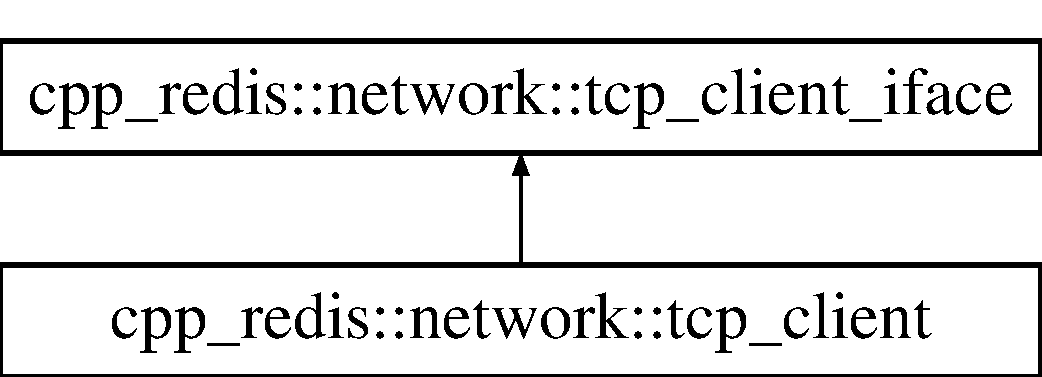
\includegraphics[height=2.000000cm]{classcpp__redis_1_1network_1_1tcp__client}
\end{center}
\end{figure}
\subsection*{Public Member Functions}
\begin{DoxyCompactItemize}
\item 
\mbox{\Hypertarget{classcpp__redis_1_1network_1_1tcp__client_a8cbad07ca636e9d60dafc0e5cac8106d}\label{classcpp__redis_1_1network_1_1tcp__client_a8cbad07ca636e9d60dafc0e5cac8106d}} 
\hyperlink{classcpp__redis_1_1network_1_1tcp__client_a8cbad07ca636e9d60dafc0e5cac8106d}{tcp\+\_\+client} (void)=default
\begin{DoxyCompactList}\small\item\em ctor \end{DoxyCompactList}\item 
\mbox{\Hypertarget{classcpp__redis_1_1network_1_1tcp__client_af859036bbc7e5ec9149c1410a1a66f09}\label{classcpp__redis_1_1network_1_1tcp__client_af859036bbc7e5ec9149c1410a1a66f09}} 
\hyperlink{classcpp__redis_1_1network_1_1tcp__client_af859036bbc7e5ec9149c1410a1a66f09}{$\sim$tcp\+\_\+client} (void)=default
\begin{DoxyCompactList}\small\item\em dtor \end{DoxyCompactList}\item 
void \hyperlink{classcpp__redis_1_1network_1_1tcp__client_a5808c0569980d83479f755ac55a12dfb}{connect} (const std\+::string \&addr, std\+::uint32\+\_\+t port, std\+::uint32\+\_\+t timeout\+\_\+msecs)
\item 
void \hyperlink{classcpp__redis_1_1network_1_1tcp__client_a88f49c4e32d59855a62296fb74136a44}{disconnect} (bool wait\+\_\+for\+\_\+removal=false)
\item 
bool \hyperlink{classcpp__redis_1_1network_1_1tcp__client_a0a636ca6bd59425bf22416a1c7694f65}{is\+\_\+connected} (void) const
\item 
void \hyperlink{classcpp__redis_1_1network_1_1tcp__client_aa56fc49540d67c5c05b3dda3aaff8a0f}{set\+\_\+nb\+\_\+workers} (std\+::size\+\_\+t nb\+\_\+threads)
\item 
void \hyperlink{classcpp__redis_1_1network_1_1tcp__client_a5eed4225fcd01e3108580d863c94c2cc}{async\+\_\+read} (\hyperlink{structcpp__redis_1_1network_1_1tcp__client__iface_1_1read__request}{read\+\_\+request} \&request)
\item 
void \hyperlink{classcpp__redis_1_1network_1_1tcp__client_a6d15785b71776cd85426c9634cb446f0}{async\+\_\+write} (\hyperlink{structcpp__redis_1_1network_1_1tcp__client__iface_1_1write__request}{write\+\_\+request} \&request)
\item 
void \hyperlink{classcpp__redis_1_1network_1_1tcp__client_a24ccdf6dc467aac13cb832a395adb38d}{set\+\_\+on\+\_\+disconnection\+\_\+handler} (const \hyperlink{classcpp__redis_1_1network_1_1tcp__client__iface_a9a7d5942205db8be03da581a848b8ec0}{disconnection\+\_\+handler\+\_\+t} \&disconnection\+\_\+handler)
\end{DoxyCompactItemize}
\subsection*{Additional Inherited Members}


\subsection{Detailed Description}
implementation of the \hyperlink{classcpp__redis_1_1network_1_1tcp__client__iface}{tcp\+\_\+client\+\_\+iface} based on tacopie networking library 

\subsection{Member Function Documentation}
\mbox{\Hypertarget{classcpp__redis_1_1network_1_1tcp__client_a5eed4225fcd01e3108580d863c94c2cc}\label{classcpp__redis_1_1network_1_1tcp__client_a5eed4225fcd01e3108580d863c94c2cc}} 
\index{cpp\+\_\+redis\+::network\+::tcp\+\_\+client@{cpp\+\_\+redis\+::network\+::tcp\+\_\+client}!async\+\_\+read@{async\+\_\+read}}
\index{async\+\_\+read@{async\+\_\+read}!cpp\+\_\+redis\+::network\+::tcp\+\_\+client@{cpp\+\_\+redis\+::network\+::tcp\+\_\+client}}
\subsubsection{\texorpdfstring{async\+\_\+read()}{async\_read()}}
{\footnotesize\ttfamily void cpp\+\_\+redis\+::network\+::tcp\+\_\+client\+::async\+\_\+read (\begin{DoxyParamCaption}\item[{\hyperlink{structcpp__redis_1_1network_1_1tcp__client__iface_1_1read__request}{read\+\_\+request} \&}]{request }\end{DoxyParamCaption})\hspace{0.3cm}{\ttfamily [virtual]}}

async read operation


\begin{DoxyParams}{Parameters}
{\em request} & information about what should be read and what should be done after completion \\
\hline
\end{DoxyParams}


Implements \hyperlink{classcpp__redis_1_1network_1_1tcp__client__iface_ae1f9fa87002273a0caf340407bb68ade}{cpp\+\_\+redis\+::network\+::tcp\+\_\+client\+\_\+iface}.

\mbox{\Hypertarget{classcpp__redis_1_1network_1_1tcp__client_a6d15785b71776cd85426c9634cb446f0}\label{classcpp__redis_1_1network_1_1tcp__client_a6d15785b71776cd85426c9634cb446f0}} 
\index{cpp\+\_\+redis\+::network\+::tcp\+\_\+client@{cpp\+\_\+redis\+::network\+::tcp\+\_\+client}!async\+\_\+write@{async\+\_\+write}}
\index{async\+\_\+write@{async\+\_\+write}!cpp\+\_\+redis\+::network\+::tcp\+\_\+client@{cpp\+\_\+redis\+::network\+::tcp\+\_\+client}}
\subsubsection{\texorpdfstring{async\+\_\+write()}{async\_write()}}
{\footnotesize\ttfamily void cpp\+\_\+redis\+::network\+::tcp\+\_\+client\+::async\+\_\+write (\begin{DoxyParamCaption}\item[{\hyperlink{structcpp__redis_1_1network_1_1tcp__client__iface_1_1write__request}{write\+\_\+request} \&}]{request }\end{DoxyParamCaption})\hspace{0.3cm}{\ttfamily [virtual]}}

async write operation


\begin{DoxyParams}{Parameters}
{\em request} & information about what should be written and what should be done after completion \\
\hline
\end{DoxyParams}


Implements \hyperlink{classcpp__redis_1_1network_1_1tcp__client__iface_a9cd01e8a68479456d15d6435ffad9b92}{cpp\+\_\+redis\+::network\+::tcp\+\_\+client\+\_\+iface}.

\mbox{\Hypertarget{classcpp__redis_1_1network_1_1tcp__client_a5808c0569980d83479f755ac55a12dfb}\label{classcpp__redis_1_1network_1_1tcp__client_a5808c0569980d83479f755ac55a12dfb}} 
\index{cpp\+\_\+redis\+::network\+::tcp\+\_\+client@{cpp\+\_\+redis\+::network\+::tcp\+\_\+client}!connect@{connect}}
\index{connect@{connect}!cpp\+\_\+redis\+::network\+::tcp\+\_\+client@{cpp\+\_\+redis\+::network\+::tcp\+\_\+client}}
\subsubsection{\texorpdfstring{connect()}{connect()}}
{\footnotesize\ttfamily void cpp\+\_\+redis\+::network\+::tcp\+\_\+client\+::connect (\begin{DoxyParamCaption}\item[{const std\+::string \&}]{addr,  }\item[{std\+::uint32\+\_\+t}]{port,  }\item[{std\+::uint32\+\_\+t}]{timeout\+\_\+msecs }\end{DoxyParamCaption})\hspace{0.3cm}{\ttfamily [virtual]}}

start the tcp client


\begin{DoxyParams}{Parameters}
{\em addr} & host to be connected to \\
\hline
{\em port} & port to be connected to \\
\hline
{\em timeout\+\_\+msecs} & max time to connect in ms \\
\hline
\end{DoxyParams}


Implements \hyperlink{classcpp__redis_1_1network_1_1tcp__client__iface_a81ee982136e85b7c3401393341bc594c}{cpp\+\_\+redis\+::network\+::tcp\+\_\+client\+\_\+iface}.

\mbox{\Hypertarget{classcpp__redis_1_1network_1_1tcp__client_a88f49c4e32d59855a62296fb74136a44}\label{classcpp__redis_1_1network_1_1tcp__client_a88f49c4e32d59855a62296fb74136a44}} 
\index{cpp\+\_\+redis\+::network\+::tcp\+\_\+client@{cpp\+\_\+redis\+::network\+::tcp\+\_\+client}!disconnect@{disconnect}}
\index{disconnect@{disconnect}!cpp\+\_\+redis\+::network\+::tcp\+\_\+client@{cpp\+\_\+redis\+::network\+::tcp\+\_\+client}}
\subsubsection{\texorpdfstring{disconnect()}{disconnect()}}
{\footnotesize\ttfamily void cpp\+\_\+redis\+::network\+::tcp\+\_\+client\+::disconnect (\begin{DoxyParamCaption}\item[{bool}]{wait\+\_\+for\+\_\+removal = {\ttfamily false} }\end{DoxyParamCaption})\hspace{0.3cm}{\ttfamily [virtual]}}

stop the tcp client


\begin{DoxyParams}{Parameters}
{\em wait\+\_\+for\+\_\+removal} & when sets to true, disconnect blocks until the underlying T\+CP client has been effectively removed from the io\+\_\+service and that all the underlying callbacks have completed. \\
\hline
\end{DoxyParams}


Implements \hyperlink{classcpp__redis_1_1network_1_1tcp__client__iface_a024073fb3436d8fa99de8cad63418f6c}{cpp\+\_\+redis\+::network\+::tcp\+\_\+client\+\_\+iface}.

\mbox{\Hypertarget{classcpp__redis_1_1network_1_1tcp__client_a0a636ca6bd59425bf22416a1c7694f65}\label{classcpp__redis_1_1network_1_1tcp__client_a0a636ca6bd59425bf22416a1c7694f65}} 
\index{cpp\+\_\+redis\+::network\+::tcp\+\_\+client@{cpp\+\_\+redis\+::network\+::tcp\+\_\+client}!is\+\_\+connected@{is\+\_\+connected}}
\index{is\+\_\+connected@{is\+\_\+connected}!cpp\+\_\+redis\+::network\+::tcp\+\_\+client@{cpp\+\_\+redis\+::network\+::tcp\+\_\+client}}
\subsubsection{\texorpdfstring{is\+\_\+connected()}{is\_connected()}}
{\footnotesize\ttfamily bool cpp\+\_\+redis\+::network\+::tcp\+\_\+client\+::is\+\_\+connected (\begin{DoxyParamCaption}\item[{void}]{ }\end{DoxyParamCaption}) const\hspace{0.3cm}{\ttfamily [virtual]}}

\begin{DoxyReturn}{Returns}
whether the client is currently connected or not 
\end{DoxyReturn}


Implements \hyperlink{classcpp__redis_1_1network_1_1tcp__client__iface_a41ad0b43e3ab172828a3d2ce55d23893}{cpp\+\_\+redis\+::network\+::tcp\+\_\+client\+\_\+iface}.

\mbox{\Hypertarget{classcpp__redis_1_1network_1_1tcp__client_aa56fc49540d67c5c05b3dda3aaff8a0f}\label{classcpp__redis_1_1network_1_1tcp__client_aa56fc49540d67c5c05b3dda3aaff8a0f}} 
\index{cpp\+\_\+redis\+::network\+::tcp\+\_\+client@{cpp\+\_\+redis\+::network\+::tcp\+\_\+client}!set\+\_\+nb\+\_\+workers@{set\+\_\+nb\+\_\+workers}}
\index{set\+\_\+nb\+\_\+workers@{set\+\_\+nb\+\_\+workers}!cpp\+\_\+redis\+::network\+::tcp\+\_\+client@{cpp\+\_\+redis\+::network\+::tcp\+\_\+client}}
\subsubsection{\texorpdfstring{set\+\_\+nb\+\_\+workers()}{set\_nb\_workers()}}
{\footnotesize\ttfamily void cpp\+\_\+redis\+::network\+::tcp\+\_\+client\+::set\+\_\+nb\+\_\+workers (\begin{DoxyParamCaption}\item[{std\+::size\+\_\+t}]{nb\+\_\+threads }\end{DoxyParamCaption})}

set number of io service workers for the io service monitoring this tcp connection


\begin{DoxyParams}{Parameters}
{\em nb\+\_\+threads} & number of threads to be assigned \\
\hline
\end{DoxyParams}
\mbox{\Hypertarget{classcpp__redis_1_1network_1_1tcp__client_a24ccdf6dc467aac13cb832a395adb38d}\label{classcpp__redis_1_1network_1_1tcp__client_a24ccdf6dc467aac13cb832a395adb38d}} 
\index{cpp\+\_\+redis\+::network\+::tcp\+\_\+client@{cpp\+\_\+redis\+::network\+::tcp\+\_\+client}!set\+\_\+on\+\_\+disconnection\+\_\+handler@{set\+\_\+on\+\_\+disconnection\+\_\+handler}}
\index{set\+\_\+on\+\_\+disconnection\+\_\+handler@{set\+\_\+on\+\_\+disconnection\+\_\+handler}!cpp\+\_\+redis\+::network\+::tcp\+\_\+client@{cpp\+\_\+redis\+::network\+::tcp\+\_\+client}}
\subsubsection{\texorpdfstring{set\+\_\+on\+\_\+disconnection\+\_\+handler()}{set\_on\_disconnection\_handler()}}
{\footnotesize\ttfamily void cpp\+\_\+redis\+::network\+::tcp\+\_\+client\+::set\+\_\+on\+\_\+disconnection\+\_\+handler (\begin{DoxyParamCaption}\item[{const \hyperlink{classcpp__redis_1_1network_1_1tcp__client__iface_a9a7d5942205db8be03da581a848b8ec0}{disconnection\+\_\+handler\+\_\+t} \&}]{disconnection\+\_\+handler }\end{DoxyParamCaption})\hspace{0.3cm}{\ttfamily [virtual]}}

set on disconnection handler


\begin{DoxyParams}{Parameters}
{\em disconnection\+\_\+handler} & handler to be called in case of a disconnection \\
\hline
\end{DoxyParams}


Implements \hyperlink{classcpp__redis_1_1network_1_1tcp__client__iface_acecf3b75c3849071d82478bc7a8c97a8}{cpp\+\_\+redis\+::network\+::tcp\+\_\+client\+\_\+iface}.



The documentation for this class was generated from the following file\+:\begin{DoxyCompactItemize}
\item 
includes/cpp\+\_\+redis/network/tcp\+\_\+client.\+hpp\end{DoxyCompactItemize}

\hypertarget{classcpp__redis_1_1network_1_1tcp__client__iface}{}\section{cpp\+\_\+redis\+:\+:network\+:\+:tcp\+\_\+client\+\_\+iface Class Reference}
\label{classcpp__redis_1_1network_1_1tcp__client__iface}\index{cpp\+\_\+redis\+::network\+::tcp\+\_\+client\+\_\+iface@{cpp\+\_\+redis\+::network\+::tcp\+\_\+client\+\_\+iface}}


{\ttfamily \#include $<$tcp\+\_\+client\+\_\+iface.\+hpp$>$}

Inheritance diagram for cpp\+\_\+redis\+:\+:network\+:\+:tcp\+\_\+client\+\_\+iface\+:\begin{figure}[H]
\begin{center}
\leavevmode
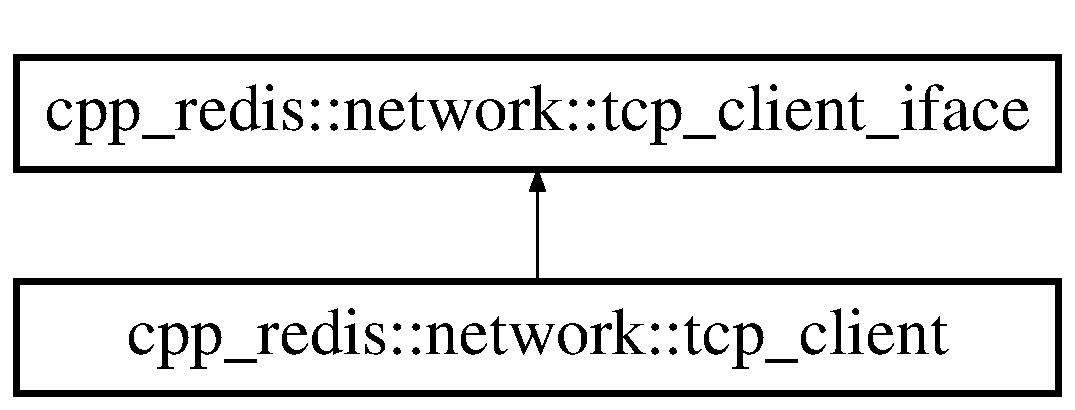
\includegraphics[height=2.000000cm]{classcpp__redis_1_1network_1_1tcp__client__iface}
\end{center}
\end{figure}
\subsection*{Classes}
\begin{DoxyCompactItemize}
\item 
struct \hyperlink{structcpp__redis_1_1network_1_1tcp__client__iface_1_1read__request}{read\+\_\+request}
\item 
struct \hyperlink{structcpp__redis_1_1network_1_1tcp__client__iface_1_1read__result}{read\+\_\+result}
\item 
struct \hyperlink{structcpp__redis_1_1network_1_1tcp__client__iface_1_1write__request}{write\+\_\+request}
\item 
struct \hyperlink{structcpp__redis_1_1network_1_1tcp__client__iface_1_1write__result}{write\+\_\+result}
\end{DoxyCompactItemize}
\subsection*{Public Types}
\begin{DoxyCompactItemize}
\item 
typedef std\+::function$<$ void(\hyperlink{structcpp__redis_1_1network_1_1tcp__client__iface_1_1read__result}{read\+\_\+result} \&)$>$ \hyperlink{classcpp__redis_1_1network_1_1tcp__client__iface_ae8bf79e8e1f1d7e359ed1c7cdc4026fc}{async\+\_\+read\+\_\+callback\+\_\+t}
\item 
typedef std\+::function$<$ void(\hyperlink{structcpp__redis_1_1network_1_1tcp__client__iface_1_1write__result}{write\+\_\+result} \&)$>$ \hyperlink{classcpp__redis_1_1network_1_1tcp__client__iface_a1dc52ccc70cf377c4fbb495a16adc658}{async\+\_\+write\+\_\+callback\+\_\+t}
\item 
typedef std\+::function$<$ void()$>$ \hyperlink{classcpp__redis_1_1network_1_1tcp__client__iface_a9a7d5942205db8be03da581a848b8ec0}{disconnection\+\_\+handler\+\_\+t}
\end{DoxyCompactItemize}
\subsection*{Public Member Functions}
\begin{DoxyCompactItemize}
\item 
\hyperlink{classcpp__redis_1_1network_1_1tcp__client__iface_a8504873049519bcebd626984e4087a90}{tcp\+\_\+client\+\_\+iface} (void)=default
\begin{DoxyCompactList}\small\item\em ctor \end{DoxyCompactList}\item 
virtual \hyperlink{classcpp__redis_1_1network_1_1tcp__client__iface_a7381e8921118a13b5994101864906122}{$\sim$tcp\+\_\+client\+\_\+iface} (void)=default
\begin{DoxyCompactList}\small\item\em dtor \end{DoxyCompactList}\item 
virtual void \hyperlink{classcpp__redis_1_1network_1_1tcp__client__iface_a81ee982136e85b7c3401393341bc594c}{connect} (const std\+::string \&addr, std\+::uint32\+\_\+t port, std\+::uint32\+\_\+t timeout\+\_\+msecs=0)=0
\item 
virtual void \hyperlink{classcpp__redis_1_1network_1_1tcp__client__iface_a024073fb3436d8fa99de8cad63418f6c}{disconnect} (bool wait\+\_\+for\+\_\+removal=false)=0
\item 
virtual bool \hyperlink{classcpp__redis_1_1network_1_1tcp__client__iface_a41ad0b43e3ab172828a3d2ce55d23893}{is\+\_\+connected} (void) const =0
\item 
virtual void \hyperlink{classcpp__redis_1_1network_1_1tcp__client__iface_ae1f9fa87002273a0caf340407bb68ade}{async\+\_\+read} (\hyperlink{structcpp__redis_1_1network_1_1tcp__client__iface_1_1read__request}{read\+\_\+request} \&request)=0
\item 
virtual void \hyperlink{classcpp__redis_1_1network_1_1tcp__client__iface_a9cd01e8a68479456d15d6435ffad9b92}{async\+\_\+write} (\hyperlink{structcpp__redis_1_1network_1_1tcp__client__iface_1_1write__request}{write\+\_\+request} \&request)=0
\item 
virtual void \hyperlink{classcpp__redis_1_1network_1_1tcp__client__iface_acecf3b75c3849071d82478bc7a8c97a8}{set\+\_\+on\+\_\+disconnection\+\_\+handler} (const \hyperlink{classcpp__redis_1_1network_1_1tcp__client__iface_a9a7d5942205db8be03da581a848b8ec0}{disconnection\+\_\+handler\+\_\+t} \&disconnection\+\_\+handler)=0
\end{DoxyCompactItemize}


\subsection{Detailed Description}
interface defining how tcp client should be implemented to be used inside \hyperlink{namespacecpp__redis}{cpp\+\_\+redis} 

\subsection{Member Typedef Documentation}
\mbox{\Hypertarget{classcpp__redis_1_1network_1_1tcp__client__iface_ae8bf79e8e1f1d7e359ed1c7cdc4026fc}\label{classcpp__redis_1_1network_1_1tcp__client__iface_ae8bf79e8e1f1d7e359ed1c7cdc4026fc}} 
\index{cpp\+\_\+redis\+::network\+::tcp\+\_\+client\+\_\+iface@{cpp\+\_\+redis\+::network\+::tcp\+\_\+client\+\_\+iface}!async\+\_\+read\+\_\+callback\+\_\+t@{async\+\_\+read\+\_\+callback\+\_\+t}}
\index{async\+\_\+read\+\_\+callback\+\_\+t@{async\+\_\+read\+\_\+callback\+\_\+t}!cpp\+\_\+redis\+::network\+::tcp\+\_\+client\+\_\+iface@{cpp\+\_\+redis\+::network\+::tcp\+\_\+client\+\_\+iface}}
\subsubsection{\texorpdfstring{async\+\_\+read\+\_\+callback\+\_\+t}{async\_read\_callback\_t}}
{\footnotesize\ttfamily typedef std\+::function$<$void(\hyperlink{structcpp__redis_1_1network_1_1tcp__client__iface_1_1read__result}{read\+\_\+result}\&)$>$ \hyperlink{classcpp__redis_1_1network_1_1tcp__client__iface_ae8bf79e8e1f1d7e359ed1c7cdc4026fc}{cpp\+\_\+redis\+::network\+::tcp\+\_\+client\+\_\+iface\+::async\+\_\+read\+\_\+callback\+\_\+t}}

async read completion callbacks function taking \hyperlink{structcpp__redis_1_1network_1_1tcp__client__iface_1_1read__result}{read\+\_\+result} as a parameter \mbox{\Hypertarget{classcpp__redis_1_1network_1_1tcp__client__iface_a1dc52ccc70cf377c4fbb495a16adc658}\label{classcpp__redis_1_1network_1_1tcp__client__iface_a1dc52ccc70cf377c4fbb495a16adc658}} 
\index{cpp\+\_\+redis\+::network\+::tcp\+\_\+client\+\_\+iface@{cpp\+\_\+redis\+::network\+::tcp\+\_\+client\+\_\+iface}!async\+\_\+write\+\_\+callback\+\_\+t@{async\+\_\+write\+\_\+callback\+\_\+t}}
\index{async\+\_\+write\+\_\+callback\+\_\+t@{async\+\_\+write\+\_\+callback\+\_\+t}!cpp\+\_\+redis\+::network\+::tcp\+\_\+client\+\_\+iface@{cpp\+\_\+redis\+::network\+::tcp\+\_\+client\+\_\+iface}}
\subsubsection{\texorpdfstring{async\+\_\+write\+\_\+callback\+\_\+t}{async\_write\_callback\_t}}
{\footnotesize\ttfamily typedef std\+::function$<$void(\hyperlink{structcpp__redis_1_1network_1_1tcp__client__iface_1_1write__result}{write\+\_\+result}\&)$>$ \hyperlink{classcpp__redis_1_1network_1_1tcp__client__iface_a1dc52ccc70cf377c4fbb495a16adc658}{cpp\+\_\+redis\+::network\+::tcp\+\_\+client\+\_\+iface\+::async\+\_\+write\+\_\+callback\+\_\+t}}

async write completion callbacks function taking \hyperlink{structcpp__redis_1_1network_1_1tcp__client__iface_1_1write__result}{write\+\_\+result} as a parameter \mbox{\Hypertarget{classcpp__redis_1_1network_1_1tcp__client__iface_a9a7d5942205db8be03da581a848b8ec0}\label{classcpp__redis_1_1network_1_1tcp__client__iface_a9a7d5942205db8be03da581a848b8ec0}} 
\index{cpp\+\_\+redis\+::network\+::tcp\+\_\+client\+\_\+iface@{cpp\+\_\+redis\+::network\+::tcp\+\_\+client\+\_\+iface}!disconnection\+\_\+handler\+\_\+t@{disconnection\+\_\+handler\+\_\+t}}
\index{disconnection\+\_\+handler\+\_\+t@{disconnection\+\_\+handler\+\_\+t}!cpp\+\_\+redis\+::network\+::tcp\+\_\+client\+\_\+iface@{cpp\+\_\+redis\+::network\+::tcp\+\_\+client\+\_\+iface}}
\subsubsection{\texorpdfstring{disconnection\+\_\+handler\+\_\+t}{disconnection\_handler\_t}}
{\footnotesize\ttfamily typedef std\+::function$<$void()$>$ \hyperlink{classcpp__redis_1_1network_1_1tcp__client__iface_a9a7d5942205db8be03da581a848b8ec0}{cpp\+\_\+redis\+::network\+::tcp\+\_\+client\+\_\+iface\+::disconnection\+\_\+handler\+\_\+t}}

disconnection handler 

\subsection{Constructor \& Destructor Documentation}
\mbox{\Hypertarget{classcpp__redis_1_1network_1_1tcp__client__iface_a8504873049519bcebd626984e4087a90}\label{classcpp__redis_1_1network_1_1tcp__client__iface_a8504873049519bcebd626984e4087a90}} 
\index{cpp\+\_\+redis\+::network\+::tcp\+\_\+client\+\_\+iface@{cpp\+\_\+redis\+::network\+::tcp\+\_\+client\+\_\+iface}!tcp\+\_\+client\+\_\+iface@{tcp\+\_\+client\+\_\+iface}}
\index{tcp\+\_\+client\+\_\+iface@{tcp\+\_\+client\+\_\+iface}!cpp\+\_\+redis\+::network\+::tcp\+\_\+client\+\_\+iface@{cpp\+\_\+redis\+::network\+::tcp\+\_\+client\+\_\+iface}}
\subsubsection{\texorpdfstring{tcp\+\_\+client\+\_\+iface()}{tcp\_client\_iface()}}
{\footnotesize\ttfamily cpp\+\_\+redis\+::network\+::tcp\+\_\+client\+\_\+iface\+::tcp\+\_\+client\+\_\+iface (\begin{DoxyParamCaption}\item[{void}]{ }\end{DoxyParamCaption})\hspace{0.3cm}{\ttfamily [default]}}



ctor 

\mbox{\Hypertarget{classcpp__redis_1_1network_1_1tcp__client__iface_a7381e8921118a13b5994101864906122}\label{classcpp__redis_1_1network_1_1tcp__client__iface_a7381e8921118a13b5994101864906122}} 
\index{cpp\+\_\+redis\+::network\+::tcp\+\_\+client\+\_\+iface@{cpp\+\_\+redis\+::network\+::tcp\+\_\+client\+\_\+iface}!````~tcp\+\_\+client\+\_\+iface@{$\sim$tcp\+\_\+client\+\_\+iface}}
\index{````~tcp\+\_\+client\+\_\+iface@{$\sim$tcp\+\_\+client\+\_\+iface}!cpp\+\_\+redis\+::network\+::tcp\+\_\+client\+\_\+iface@{cpp\+\_\+redis\+::network\+::tcp\+\_\+client\+\_\+iface}}
\subsubsection{\texorpdfstring{$\sim$tcp\+\_\+client\+\_\+iface()}{~tcp\_client\_iface()}}
{\footnotesize\ttfamily virtual cpp\+\_\+redis\+::network\+::tcp\+\_\+client\+\_\+iface\+::$\sim$tcp\+\_\+client\+\_\+iface (\begin{DoxyParamCaption}\item[{void}]{ }\end{DoxyParamCaption})\hspace{0.3cm}{\ttfamily [virtual]}, {\ttfamily [default]}}



dtor 



\subsection{Member Function Documentation}
\mbox{\Hypertarget{classcpp__redis_1_1network_1_1tcp__client__iface_ae1f9fa87002273a0caf340407bb68ade}\label{classcpp__redis_1_1network_1_1tcp__client__iface_ae1f9fa87002273a0caf340407bb68ade}} 
\index{cpp\+\_\+redis\+::network\+::tcp\+\_\+client\+\_\+iface@{cpp\+\_\+redis\+::network\+::tcp\+\_\+client\+\_\+iface}!async\+\_\+read@{async\+\_\+read}}
\index{async\+\_\+read@{async\+\_\+read}!cpp\+\_\+redis\+::network\+::tcp\+\_\+client\+\_\+iface@{cpp\+\_\+redis\+::network\+::tcp\+\_\+client\+\_\+iface}}
\subsubsection{\texorpdfstring{async\+\_\+read()}{async\_read()}}
{\footnotesize\ttfamily virtual void cpp\+\_\+redis\+::network\+::tcp\+\_\+client\+\_\+iface\+::async\+\_\+read (\begin{DoxyParamCaption}\item[{\hyperlink{structcpp__redis_1_1network_1_1tcp__client__iface_1_1read__request}{read\+\_\+request} \&}]{request }\end{DoxyParamCaption})\hspace{0.3cm}{\ttfamily [pure virtual]}}

async read operation


\begin{DoxyParams}{Parameters}
{\em request} & information about what should be read and what should be done after completion \\
\hline
\end{DoxyParams}


Implemented in \hyperlink{classcpp__redis_1_1network_1_1tcp__client_a5eed4225fcd01e3108580d863c94c2cc}{cpp\+\_\+redis\+::network\+::tcp\+\_\+client}.

\mbox{\Hypertarget{classcpp__redis_1_1network_1_1tcp__client__iface_a9cd01e8a68479456d15d6435ffad9b92}\label{classcpp__redis_1_1network_1_1tcp__client__iface_a9cd01e8a68479456d15d6435ffad9b92}} 
\index{cpp\+\_\+redis\+::network\+::tcp\+\_\+client\+\_\+iface@{cpp\+\_\+redis\+::network\+::tcp\+\_\+client\+\_\+iface}!async\+\_\+write@{async\+\_\+write}}
\index{async\+\_\+write@{async\+\_\+write}!cpp\+\_\+redis\+::network\+::tcp\+\_\+client\+\_\+iface@{cpp\+\_\+redis\+::network\+::tcp\+\_\+client\+\_\+iface}}
\subsubsection{\texorpdfstring{async\+\_\+write()}{async\_write()}}
{\footnotesize\ttfamily virtual void cpp\+\_\+redis\+::network\+::tcp\+\_\+client\+\_\+iface\+::async\+\_\+write (\begin{DoxyParamCaption}\item[{\hyperlink{structcpp__redis_1_1network_1_1tcp__client__iface_1_1write__request}{write\+\_\+request} \&}]{request }\end{DoxyParamCaption})\hspace{0.3cm}{\ttfamily [pure virtual]}}

async write operation


\begin{DoxyParams}{Parameters}
{\em request} & information about what should be written and what should be done after completion \\
\hline
\end{DoxyParams}


Implemented in \hyperlink{classcpp__redis_1_1network_1_1tcp__client_a6d15785b71776cd85426c9634cb446f0}{cpp\+\_\+redis\+::network\+::tcp\+\_\+client}.

\mbox{\Hypertarget{classcpp__redis_1_1network_1_1tcp__client__iface_a81ee982136e85b7c3401393341bc594c}\label{classcpp__redis_1_1network_1_1tcp__client__iface_a81ee982136e85b7c3401393341bc594c}} 
\index{cpp\+\_\+redis\+::network\+::tcp\+\_\+client\+\_\+iface@{cpp\+\_\+redis\+::network\+::tcp\+\_\+client\+\_\+iface}!connect@{connect}}
\index{connect@{connect}!cpp\+\_\+redis\+::network\+::tcp\+\_\+client\+\_\+iface@{cpp\+\_\+redis\+::network\+::tcp\+\_\+client\+\_\+iface}}
\subsubsection{\texorpdfstring{connect()}{connect()}}
{\footnotesize\ttfamily virtual void cpp\+\_\+redis\+::network\+::tcp\+\_\+client\+\_\+iface\+::connect (\begin{DoxyParamCaption}\item[{const std\+::string \&}]{addr,  }\item[{std\+::uint32\+\_\+t}]{port,  }\item[{std\+::uint32\+\_\+t}]{timeout\+\_\+msecs = {\ttfamily 0} }\end{DoxyParamCaption})\hspace{0.3cm}{\ttfamily [pure virtual]}}

start the tcp client


\begin{DoxyParams}{Parameters}
{\em addr} & host to be connected to \\
\hline
{\em port} & port to be connected to \\
\hline
{\em timeout\+\_\+msecs} & max time to connect in ms \\
\hline
\end{DoxyParams}


Implemented in \hyperlink{classcpp__redis_1_1network_1_1tcp__client_a5808c0569980d83479f755ac55a12dfb}{cpp\+\_\+redis\+::network\+::tcp\+\_\+client}.

\mbox{\Hypertarget{classcpp__redis_1_1network_1_1tcp__client__iface_a024073fb3436d8fa99de8cad63418f6c}\label{classcpp__redis_1_1network_1_1tcp__client__iface_a024073fb3436d8fa99de8cad63418f6c}} 
\index{cpp\+\_\+redis\+::network\+::tcp\+\_\+client\+\_\+iface@{cpp\+\_\+redis\+::network\+::tcp\+\_\+client\+\_\+iface}!disconnect@{disconnect}}
\index{disconnect@{disconnect}!cpp\+\_\+redis\+::network\+::tcp\+\_\+client\+\_\+iface@{cpp\+\_\+redis\+::network\+::tcp\+\_\+client\+\_\+iface}}
\subsubsection{\texorpdfstring{disconnect()}{disconnect()}}
{\footnotesize\ttfamily virtual void cpp\+\_\+redis\+::network\+::tcp\+\_\+client\+\_\+iface\+::disconnect (\begin{DoxyParamCaption}\item[{bool}]{wait\+\_\+for\+\_\+removal = {\ttfamily false} }\end{DoxyParamCaption})\hspace{0.3cm}{\ttfamily [pure virtual]}}

stop the tcp client


\begin{DoxyParams}{Parameters}
{\em wait\+\_\+for\+\_\+removal} & when sets to true, disconnect blocks until the underlying T\+CP client has been effectively removed from the io\+\_\+service and that all the underlying callbacks have completed. \\
\hline
\end{DoxyParams}


Implemented in \hyperlink{classcpp__redis_1_1network_1_1tcp__client_a88f49c4e32d59855a62296fb74136a44}{cpp\+\_\+redis\+::network\+::tcp\+\_\+client}.

\mbox{\Hypertarget{classcpp__redis_1_1network_1_1tcp__client__iface_a41ad0b43e3ab172828a3d2ce55d23893}\label{classcpp__redis_1_1network_1_1tcp__client__iface_a41ad0b43e3ab172828a3d2ce55d23893}} 
\index{cpp\+\_\+redis\+::network\+::tcp\+\_\+client\+\_\+iface@{cpp\+\_\+redis\+::network\+::tcp\+\_\+client\+\_\+iface}!is\+\_\+connected@{is\+\_\+connected}}
\index{is\+\_\+connected@{is\+\_\+connected}!cpp\+\_\+redis\+::network\+::tcp\+\_\+client\+\_\+iface@{cpp\+\_\+redis\+::network\+::tcp\+\_\+client\+\_\+iface}}
\subsubsection{\texorpdfstring{is\+\_\+connected()}{is\_connected()}}
{\footnotesize\ttfamily virtual bool cpp\+\_\+redis\+::network\+::tcp\+\_\+client\+\_\+iface\+::is\+\_\+connected (\begin{DoxyParamCaption}\item[{void}]{ }\end{DoxyParamCaption}) const\hspace{0.3cm}{\ttfamily [pure virtual]}}

\begin{DoxyReturn}{Returns}
whether the client is currently connected or not 
\end{DoxyReturn}


Implemented in \hyperlink{classcpp__redis_1_1network_1_1tcp__client_a0a636ca6bd59425bf22416a1c7694f65}{cpp\+\_\+redis\+::network\+::tcp\+\_\+client}.

\mbox{\Hypertarget{classcpp__redis_1_1network_1_1tcp__client__iface_acecf3b75c3849071d82478bc7a8c97a8}\label{classcpp__redis_1_1network_1_1tcp__client__iface_acecf3b75c3849071d82478bc7a8c97a8}} 
\index{cpp\+\_\+redis\+::network\+::tcp\+\_\+client\+\_\+iface@{cpp\+\_\+redis\+::network\+::tcp\+\_\+client\+\_\+iface}!set\+\_\+on\+\_\+disconnection\+\_\+handler@{set\+\_\+on\+\_\+disconnection\+\_\+handler}}
\index{set\+\_\+on\+\_\+disconnection\+\_\+handler@{set\+\_\+on\+\_\+disconnection\+\_\+handler}!cpp\+\_\+redis\+::network\+::tcp\+\_\+client\+\_\+iface@{cpp\+\_\+redis\+::network\+::tcp\+\_\+client\+\_\+iface}}
\subsubsection{\texorpdfstring{set\+\_\+on\+\_\+disconnection\+\_\+handler()}{set\_on\_disconnection\_handler()}}
{\footnotesize\ttfamily virtual void cpp\+\_\+redis\+::network\+::tcp\+\_\+client\+\_\+iface\+::set\+\_\+on\+\_\+disconnection\+\_\+handler (\begin{DoxyParamCaption}\item[{const \hyperlink{classcpp__redis_1_1network_1_1tcp__client__iface_a9a7d5942205db8be03da581a848b8ec0}{disconnection\+\_\+handler\+\_\+t} \&}]{disconnection\+\_\+handler }\end{DoxyParamCaption})\hspace{0.3cm}{\ttfamily [pure virtual]}}

set on disconnection handler


\begin{DoxyParams}{Parameters}
{\em disconnection\+\_\+handler} & handler to be called in case of a disconnection \\
\hline
\end{DoxyParams}


Implemented in \hyperlink{classcpp__redis_1_1network_1_1tcp__client_a24ccdf6dc467aac13cb832a395adb38d}{cpp\+\_\+redis\+::network\+::tcp\+\_\+client}.



The documentation for this class was generated from the following file\+:\begin{DoxyCompactItemize}
\item 
includes/cpp\+\_\+redis/network/\hyperlink{tcp__client__iface_8hpp}{tcp\+\_\+client\+\_\+iface.\+hpp}\end{DoxyCompactItemize}

\hypertarget{structcpp__redis_1_1network_1_1tcp__client__iface_1_1write__request}{}\section{cpp\+\_\+redis\+:\+:network\+:\+:tcp\+\_\+client\+\_\+iface\+:\+:write\+\_\+request Struct Reference}
\label{structcpp__redis_1_1network_1_1tcp__client__iface_1_1write__request}\index{cpp\+\_\+redis\+::network\+::tcp\+\_\+client\+\_\+iface\+::write\+\_\+request@{cpp\+\_\+redis\+::network\+::tcp\+\_\+client\+\_\+iface\+::write\+\_\+request}}


{\ttfamily \#include $<$tcp\+\_\+client\+\_\+iface.\+hpp$>$}

\subsection*{Public Attributes}
\begin{DoxyCompactItemize}
\item 
std\+::vector$<$ char $>$ \hyperlink{structcpp__redis_1_1network_1_1tcp__client__iface_1_1write__request_ad3567dac827f550b60491af530f0db2e}{buffer}
\item 
\hyperlink{classcpp__redis_1_1network_1_1tcp__client__iface_a1dc52ccc70cf377c4fbb495a16adc658}{async\+\_\+write\+\_\+callback\+\_\+t} \hyperlink{structcpp__redis_1_1network_1_1tcp__client__iface_1_1write__request_ab2823d9836ec68d63c9799ee12d403a2}{async\+\_\+write\+\_\+callback}
\end{DoxyCompactItemize}


\subsection{Detailed Description}
structure to store write requests information 

\subsection{Member Data Documentation}
\mbox{\Hypertarget{structcpp__redis_1_1network_1_1tcp__client__iface_1_1write__request_ab2823d9836ec68d63c9799ee12d403a2}\label{structcpp__redis_1_1network_1_1tcp__client__iface_1_1write__request_ab2823d9836ec68d63c9799ee12d403a2}} 
\index{cpp\+\_\+redis\+::network\+::tcp\+\_\+client\+\_\+iface\+::write\+\_\+request@{cpp\+\_\+redis\+::network\+::tcp\+\_\+client\+\_\+iface\+::write\+\_\+request}!async\+\_\+write\+\_\+callback@{async\+\_\+write\+\_\+callback}}
\index{async\+\_\+write\+\_\+callback@{async\+\_\+write\+\_\+callback}!cpp\+\_\+redis\+::network\+::tcp\+\_\+client\+\_\+iface\+::write\+\_\+request@{cpp\+\_\+redis\+::network\+::tcp\+\_\+client\+\_\+iface\+::write\+\_\+request}}
\subsubsection{\texorpdfstring{async\+\_\+write\+\_\+callback}{async\_write\_callback}}
{\footnotesize\ttfamily \hyperlink{classcpp__redis_1_1network_1_1tcp__client__iface_a1dc52ccc70cf377c4fbb495a16adc658}{async\+\_\+write\+\_\+callback\+\_\+t} cpp\+\_\+redis\+::network\+::tcp\+\_\+client\+\_\+iface\+::write\+\_\+request\+::async\+\_\+write\+\_\+callback}

callback to be called on operation completion \mbox{\Hypertarget{structcpp__redis_1_1network_1_1tcp__client__iface_1_1write__request_ad3567dac827f550b60491af530f0db2e}\label{structcpp__redis_1_1network_1_1tcp__client__iface_1_1write__request_ad3567dac827f550b60491af530f0db2e}} 
\index{cpp\+\_\+redis\+::network\+::tcp\+\_\+client\+\_\+iface\+::write\+\_\+request@{cpp\+\_\+redis\+::network\+::tcp\+\_\+client\+\_\+iface\+::write\+\_\+request}!buffer@{buffer}}
\index{buffer@{buffer}!cpp\+\_\+redis\+::network\+::tcp\+\_\+client\+\_\+iface\+::write\+\_\+request@{cpp\+\_\+redis\+::network\+::tcp\+\_\+client\+\_\+iface\+::write\+\_\+request}}
\subsubsection{\texorpdfstring{buffer}{buffer}}
{\footnotesize\ttfamily std\+::vector$<$char$>$ cpp\+\_\+redis\+::network\+::tcp\+\_\+client\+\_\+iface\+::write\+\_\+request\+::buffer}

bytes to write 

The documentation for this struct was generated from the following file\+:\begin{DoxyCompactItemize}
\item 
includes/cpp\+\_\+redis/network/tcp\+\_\+client\+\_\+iface.\+hpp\end{DoxyCompactItemize}

\hypertarget{structcpp__redis_1_1network_1_1tcp__client__iface_1_1write__result}{}\section{cpp\+\_\+redis\+:\+:network\+:\+:tcp\+\_\+client\+\_\+iface\+:\+:write\+\_\+result Struct Reference}
\label{structcpp__redis_1_1network_1_1tcp__client__iface_1_1write__result}\index{cpp\+\_\+redis\+::network\+::tcp\+\_\+client\+\_\+iface\+::write\+\_\+result@{cpp\+\_\+redis\+::network\+::tcp\+\_\+client\+\_\+iface\+::write\+\_\+result}}


{\ttfamily \#include $<$tcp\+\_\+client\+\_\+iface.\+hpp$>$}

\subsection*{Public Attributes}
\begin{DoxyCompactItemize}
\item 
bool \hyperlink{structcpp__redis_1_1network_1_1tcp__client__iface_1_1write__result_a677696941c9a7164bc0b93b5d8380d1a}{success}
\item 
std\+::size\+\_\+t \hyperlink{structcpp__redis_1_1network_1_1tcp__client__iface_1_1write__result_a580f3dbe5ea3f6f4b6b4ca0bfad2c06c}{size}
\end{DoxyCompactItemize}


\subsection{Detailed Description}
structure to store write requests result 

\subsection{Member Data Documentation}
\mbox{\Hypertarget{structcpp__redis_1_1network_1_1tcp__client__iface_1_1write__result_a580f3dbe5ea3f6f4b6b4ca0bfad2c06c}\label{structcpp__redis_1_1network_1_1tcp__client__iface_1_1write__result_a580f3dbe5ea3f6f4b6b4ca0bfad2c06c}} 
\index{cpp\+\_\+redis\+::network\+::tcp\+\_\+client\+\_\+iface\+::write\+\_\+result@{cpp\+\_\+redis\+::network\+::tcp\+\_\+client\+\_\+iface\+::write\+\_\+result}!size@{size}}
\index{size@{size}!cpp\+\_\+redis\+::network\+::tcp\+\_\+client\+\_\+iface\+::write\+\_\+result@{cpp\+\_\+redis\+::network\+::tcp\+\_\+client\+\_\+iface\+::write\+\_\+result}}
\subsubsection{\texorpdfstring{size}{size}}
{\footnotesize\ttfamily std\+::size\+\_\+t cpp\+\_\+redis\+::network\+::tcp\+\_\+client\+\_\+iface\+::write\+\_\+result\+::size}

number of bytes written \mbox{\Hypertarget{structcpp__redis_1_1network_1_1tcp__client__iface_1_1write__result_a677696941c9a7164bc0b93b5d8380d1a}\label{structcpp__redis_1_1network_1_1tcp__client__iface_1_1write__result_a677696941c9a7164bc0b93b5d8380d1a}} 
\index{cpp\+\_\+redis\+::network\+::tcp\+\_\+client\+\_\+iface\+::write\+\_\+result@{cpp\+\_\+redis\+::network\+::tcp\+\_\+client\+\_\+iface\+::write\+\_\+result}!success@{success}}
\index{success@{success}!cpp\+\_\+redis\+::network\+::tcp\+\_\+client\+\_\+iface\+::write\+\_\+result@{cpp\+\_\+redis\+::network\+::tcp\+\_\+client\+\_\+iface\+::write\+\_\+result}}
\subsubsection{\texorpdfstring{success}{success}}
{\footnotesize\ttfamily bool cpp\+\_\+redis\+::network\+::tcp\+\_\+client\+\_\+iface\+::write\+\_\+result\+::success}

whether the operation succeeded or not 

The documentation for this struct was generated from the following file\+:\begin{DoxyCompactItemize}
\item 
includes/cpp\+\_\+redis/network/tcp\+\_\+client\+\_\+iface.\+hpp\end{DoxyCompactItemize}

%--- End generated contents ---

% Index
\backmatter
\newpage
\phantomsection
\clearemptydoublepage
\addcontentsline{toc}{chapter}{Index}
\printindex

\end{document}
